%!TEX TS-program = xelatex
%!TEX encoding = UTF-8

% Cumulative Indonesian reader for Methods of Algebra, Volume 2.
% Upstream source: Wen-Wei Li, CC BY 4.0.
\documentclass[
  colors=true,
  fontsetup=font-setup-id.tex,
  titlesetup=titles-setup.tex
]{AJbook2}

% Localize inherited chapter labels without modifying the exact upstream
% title-style support file.
\renewcommand{\AJchapterttl}[1]{%
  \IfSubStr{ABCDEFGHIJKLMNOPQRSTUVWXYZ}{#1}{Lampiran #1}{Bab #1}}
\renewcommand{\MakeChapBox}[2]{%
  \begin{tcolorbox}[
    enhanced jigsaw,
    skin=bicolor,
    frame engine=path,
    sharp corners=all,
    width=\dimexpr\textwidth-1pc\relax,
    top=5mm,
    bottom=5mm,
    sidebyside,
    frame hidden,
    boxrule=0mm,
    lefthand width=0.20\textwidth,
    colupper=white,
    colback=gray!72,
    colbacklower=gray!8,
    sidebyside align=center,
    halign=center,
    halign lower=center]
    {\Large\bfseries\AJchapterttl{#1}}
    \tcblower
    {\LARGE\bfseries #2}
  \end{tcolorbox}}
\AtBeginDocument{%
  \renewcommand{\chaptermark}[1]{\markboth{Bab \thechapter\quad #1}{}}}

% Provide Indonesian theorem chrome while preserving the upstream theorem
% counter and all source labels. The upstream environments remain available
% for source comparison but are not used on the localized reader surface.
\AtBeginDocument{%
  \theoremstyle{plain}
  \theorembodyfont{\normalfont}
  \theoremheaderfont{\sffamily\bfseries}
  \theoremseparator{\ }
  \theoremsymbol{}
  \newtheorem{teorema}[theorem]{Teorema}
  \newtheorem{korolari}[theorem]{Korolari}
  \newtheorem{lema}[theorem]{Lema}
  \newtheorem{proposisi}[theorem]{Proposisi}
  \newtheorem{definisi}[theorem]{Definisi}
  \newtheorem{definisiteorema}[theorem]{Definisi--Teorema}
  \newtheorem{definisiproposisi}[theorem]{Definisi--Proposisi}
  \newtheorem{hipotesis}[theorem]{Hipotesis}
  \newtheorem{konjektur}[theorem]{Konjektur}
  \newtheorem{contoh}[theorem]{Contoh}
  \newtheorem{catatan}[theorem]{Catatan}
  \newtheorem{konvensi}[theorem]{Konvensi}
  \newtheorem{latihan}[theorem]{Latihan}
  \theorembodyfont{\normalfont}
  \theoremstyle{nonumberplain}
  \theoremheaderfont{\sffamily\bfseries}
  \theoremseparator{\enspace}
  \theoremsymbol{\ensuremath{\square}}
  \newtheorem{bukti}{Bukti}}

\usepackage{mathrsfs}
\usepackage{stmaryrd}
\SetSymbolFont{stmry}{bold}{U}{stmry}{m}{n}
\usepackage{array}
\usepackage{tikz-cd}
\usetikzlibrary{fit}
\usepackage{mycommand}
% Unit 011 first needs the upstream \xlongequal implementation. Preserve the
% standard extendable arrows used by earlier units rather than applying the
% support package's global redefinitions retroactively.
\let\OOriginalXrightarrow\xrightarrow
\let\OOriginalXleftarrow\xleftarrow
\let\OOriginalXleftrightarrow\xleftrightarrow
\let\OOriginalXhookrightarrow\xhookrightarrow
\let\OOriginalXhookleftarrow\xhookleftarrow
\let\OOriginalXmapsto\xmapsto
\usepackage{myarrows}
\let\xrightarrow\OOriginalXrightarrow
\let\xleftarrow\OOriginalXleftarrow
\let\xleftrightarrow\OOriginalXleftrightarrow
\let\xhookrightarrow\OOriginalXhookrightarrow
\let\xhookleftarrow\OOriginalXhookleftarrow
\let\xmapsto\OOriginalXmapsto
\numberwithin{equation}{section}
\numberwithin{figure}{section}
\usepackage[unicode,bookmarksnumbered]{hyperref}
% Resolve source cross-references when their target is present; otherwise show
% the frozen source designation without emitting a broken partial-reader link.
\makeatletter
\newcommand{\sourcecrossref}[2]{\@ifundefined{r@#1}{#2}{\ref{#1}}}
\makeatother
% Localize the class's chapter-end exercise and inline-hint chrome without
% modifying the byte-exact upstream AJbook2.cls support file.
\renewenvironment{Exercises}{%
  \markright{Latihan}%
  \addcontentsline{toc}{section}{Latihan}%
  \vspace{1em}\begin{center}%
    \Large\bfseries Latihan%
  \end{center}\vspace{0.7em}%
  \begin{small}\begin{enumerate}[\bfseries 1.]%
}{%
  \end{enumerate}\end{small}%
}
\renewenvironment{hint}{%
  \ifvmode
    \ignorespaces
  \else
    \quad
  \fi
  \begin{tikzpicture}[baseline=(H.base), every node/.style={signal, draw,
    very thin, signal to=east, signal from=nowhere,
    signal pointer angle=120, inner sep=2pt}]
    \node[anchor=mid west] (H) at (0,0)
      {\sffamily\footnotesize Petunjuk};
  \end{tikzpicture}%
}{}
\hypersetup{
  pdflang={id-ID},
  pdfauthor={Wen-Wei Li; terjemahan Bahasa Indonesia oleh Codex atas instruksi pengguna},
  pdftitle={Metode dalam Aljabar, Jilid 2 - Pembaca Kumulatif Bahasa Indonesia},
  pdfsubject={Pendahuluan lengkap, Bab 1 lengkap, Bab 2 lengkap, dan Bab 3 sampai Bagian 3.9},
  pdfkeywords={aljabar homologis, teori kategori, Bahasa Indonesia}
}
\usepackage[open,openlevel=0]{bookmark}
\usepackage{imakeidx}
\makeindex[title={Indeks Istilah},columns=2,intoc=true]
\makeindex[name=sym1,title={Indeks Simbol},columns=3,intoc=true]
\addbibresource{references-cumulative-through-unit-040.bib}
\ExecuteBibliographyOptions{backref=false}
\DefineBibliographyStrings{english}{%
  in={dalam},
  editor={editor},
  byeditor={disunting oleh},
  backrefpage={dikutip pada hlm.\!},
  backrefpages={dikutip pada hlm.\!}
}
\setlength{\emergencystretch}{1.5em}
\newtcolorbox{petunjukbacaan}{
  breakable,
  enhanced,
  width=\textwidth,
  colback=white,
  colbacktitle=white,
  colframe=gray!50,
  boxrule=0.2mm,
  coltitle=black,
  fonttitle=\sffamily,
  attach boxed title to top left={yshift=-\tcboxedtitleheight/2,xshift=\tcboxedtitlewidth/4},
  boxed title style={boxrule=0pt,colframe=white},
  before skip=0.5cm,
  top=3mm,
  bottom=3mm,
  title={Petunjuk Bacaan}
}

\begin{document}

\begin{titlepage}
  \centering
  \vspace*{0.16\textheight}
  {\Huge\bfseries Metode dalam Aljabar\par}
  \vspace{0.8em}
  {\LARGE Jilid 2\par}
  \vspace{1.8em}
  {\Large Pembaca Kumulatif Bahasa Indonesia\par}
  \vspace{0.6em}
  {\large Pendahuluan Lengkap, Bab 1 Lengkap, Bab 2 Lengkap, dan Bab 3 sampai Bagian 3.9\par}
  \vfill
  {\Large Wen-Wei Li\par}
  \vspace{0.6em}
  {\normalsize Terjemahan independen Bahasa Indonesia\par}
  \vspace*{0.10\textheight}
\end{titlepage}

\cleardoublepage
\thispagestyle{empty}
\section*{Atribusi dan status pembaca}
Karya sumber: Wen-Wei Li, \emph{Methods of Algebra, Volume 2}. Versi
sumber dibekukan pada commit berikut:
\begin{center}
  \small
  \href{https://github.com/wenweili/AlJabr-2}{\texttt{github.com/wenweili/AlJabr-2}}\\
  \href{https://github.com/wenweili/AlJabr-2/commit/9a5803ff77dd3257484cb177f851a73770a59dd3}{\texttt{commit 9a5803ff77dd3257484cb177f851a73770a59dd3}}
\end{center}
Kode sumber upstream dan turunannya berlisensi Creative Commons
Attribution 4.0 International (CC BY 4.0):
\begin{center}
  \small\url{https://creativecommons.org/licenses/by/4.0/}
\end{center}
Pembaca ini menerjemahkan
\texttt{prelude.tex} baris 9--495, \texttt{chapter1.tex} baris 9--2079,
serta \texttt{chapter2.tex} baris 9--2132 dan \texttt{chapter3.tex} baris
9--1708, serta menandai perubahan bahasa dan penyajian secara eksplisit. Wen-Wei Li dan penerbit sumber tidak
mendukung atau mengesahkan terjemahan independen ini.

\medskip
Teks sumber, notasi matematika, sitasi, dan struktur konseptual tetap
diatribusikan kepada Wen-Wei Li. Metadata pembaca dan label stabil lokal
ditambahkan hanya untuk produksi pembaca Bahasa Indonesia.

\medskip
Provenans produksi: terjemahan Bahasa Indonesia, rekonsiliasi terminologi,
metadata, backend modular, dan QA diproduksi dengan
\textbf{OpenAI Codex gpt-5.6-sol, Ultra}, atas arahan pengguna. Pengungkapan ini tidak menggantikan
kredit Wen-Wei Li sebagai penulis karya sumber atau kredit komponen lain.

\cleardoublepage
\renewcommand{\contentsname}{Daftar Isi}
\tableofcontents
\mainmatter

% Terjemahan Bahasa Indonesia dari prelude.tex baris 9-29.
% Sumber: Methods of Algebra, Volume 2, commit
% 9a5803ff77dd3257484cb177f851a73770a59dd3 (CC BY 4.0).
% stable-unit-id: o014.aljabr2.prelude.linear-algebra

\chapter*{Pendahuluan}
\hypertarget{o014.aljabr2.prelude}{ }

% segment-id: o014.li2.prelude.p001
Karya yang disajikan kepada pembaca ini merupakan kelanjutan dari
\cite{Li1} (selanjutnya disebut Jilid I). Tujuannya adalah memperkenalkan
serangkaian metode, gagasan, dan teknik yang secara wajar dapat dihimpun
di bawah nama aljabar linear, dengan mengandaikan bahwa pembaca telah
mengenal struktur-struktur dasar dalam aljabar. Metode-metode ini dipakai
di seluruh matematika kontemporer. Agar dapat menjawab kebutuhan praktis
sekomprehensif mungkin, teknik-teknik terkait perlu ditempa menjadi bentuk yang
lebih murni dan lebih ringkas. Kategori dan funktor merupakan bahasa yang
tak tergantikan untuk tujuan tersebut.

% segment-id: o014.li2.prelude.p002
Buku ini terbagi menjadi tiga bagian: bagian dalam, bagian luar,
dan lampiran. Sasaran utamanya ialah mahasiswa sarjana tingkat lanjut,
mahasiswa pascasarjana, peneliti, pengajar, dan pembelajar mandiri yang
menekuni atau berminat pada pokok-pokok ini. Pengetahuan prasyaratnya
mencakup grup, gelanggang, modul, lapangan, dan struktur aljabar lain, serta
teori kategori. Jilid I mencakup seluruh landasan tersebut, tetapi buku
teks bermutu lainnya juga memadai, meskipun mungkin terdapat sedikit
perbedaan notasi.
Motivasi penulisan telah dijelaskan dalam pendahuluan Jilid I; tujuannya
tetap sama dan tidak perlu diulang di sini.

\section*{Apakah Aljabar Linear Itu?}
\addcontentsline{toc}{section}{Apakah Aljabar Linear Itu?}
\hypertarget{o014.aljabr2.prelude.linear-algebra}{ }
\index{aljabar linear (linear algebra)}

% segment-id: o014.li2.prelude.linear-algebra.p001
Dalam pengertian yang lazim di kalangan ahli aljabar, kata ``linear''
secara luas merujuk pada sifat-sifat yang berhubungan dengan struktur
yang memiliki penjumlahan beserta operasi inversnya, yaitu pengurangan.
Penjumlahan dan pengurangan selanjutnya memberikan operasi perkalian
dengan bilangan bulat; generalisasi langsungnya adalah perkalian skalar
oleh unsur suatu gelanggang $R$. Contoh prototipikalnya ialah modul kiri
dan modul kanan atas $R$, sedangkan modul-$\Z$ tidak lain adalah grup
abelian. Untuk suatu modul-$R$ (mulai sekarang modul kiri, kecuali dinyatakan
lain), kita dapat mempelajari submodul dan modul kuosien (modul hasil bagi),
serta kernel
$\Ker(f)$, kokernel $\Coker(f)$, dan citra $\Image(f)$ dari suatu
homomorfisme modul $f$. Semuanya merupakan objek yang sudah dikenal dari
aljabar dasar; setidaknya, kasus ketika $R$ adalah lapangan, yakni kasus
ruang vektor, telah dikenal luas.

% segment-id: o014.li2.prelude.linear-algebra.p002
Sejak abad ke-20, praktik matematika secara bertahap memperlihatkan bahwa
memperluas kajian modul-$R$ dan homomorfismenya ke kompleks modul bukan
hanya bermanfaat dan memudahkan, melainkan sering kali diperlukan.
Kompleks semacam itu adalah deretan homomorfisme modul yang memenuhi
$d^{n+1}d^n=0$:
\[
  \cdots \longrightarrow X^{n-1} \xrightarrow{d^{n-1}} X^n
  \xrightarrow{d^n} X^{n+1} \xrightarrow{d^{n+1}} \cdots .
\]
Syarat pada homomorfisme tersebut kadang ditulis $d^2=0$, sedangkan
seluruh data kompleks sering disingkat menjadi $(X^n,d^n)_n$, $(X,d)$,
atau $X$. Karena digunakan indeks atas yang meningkat, kompleks ini juga
disebut kompleks kokrantai (\emph{cochain complex}). Jika digunakan indeks
bawah yang menurun,
$\cdots\to X_n\xrightarrow{d_n}X_{n-1}\to\cdots$, objek matematis yang
diperoleh disebut kompleks rantai; perbedaannya dengan kompleks di atas
hanya bersifat formal.

% segment-id: o014.li2.prelude.linear-algebra.p003
Suatu modul-$R$ tunggal $M$ dapat dipandang sebagai kasus khusus kompleks,
dengan $X^0=M$ dan semua suku lainnya nol. Untuk suatu kompleks $X$,
karena $d^nd^{n-1}=0$, kohomologi ke-$n$ dapat didefinisikan sebagai
modul kuosien
\[
  \Hm^n(X):=\Ker\left(d^n\right)\big/\Image\left(d^{n-1}\right).
\]

% segment-id: o014.li2.prelude.linear-algebra.p004
Kompleks yang memenuhi $\Hm^n(X)=0$ untuk setiap $n$ disebut barisan
eksak atau kompleks asiklik. Untuk kompleks rantai, secara bersesuaian
kita memiliki homologi
$\Hm_n(X):=\Ker(d_n)/\Image(d_{n+1})$. Kohomologi suatu kompleks (atau
homologi suatu kompleks rantai) sering menyimpan informasi penting
tentang objek matematis yang dikaji.

\enlargethispage{3\baselineskip}
% segment-id: o014.li2.prelude.linear-algebra.p005
Untuk modul atau struktur matematis lain yang memiliki operasi linear,
misalnya objek dalam kategori abelian yang akan diperkenalkan kemudian,
kajian kompleks beserta kohomologinya merupakan isi klasik bidang yang
disebut aljabar homologis. Bidang ini merupakan subhimpunan sejati dari
``aljabar linear'' dalam arti hakikinya dan sekaligus merupakan inti buku
ini. Riwayat singkatnya akan dibahas berikutnya.

% Terjemahan Bahasa Indonesia dari prelude.tex baris 30-103.
% Sumber: Methods of Algebra, Volume 2, commit
% 9a5803ff77dd3257484cb177f851a73770a59dd3 (CC BY 4.0).
% stable-unit-id: o014.aljabr2.prelude.homology-history

\section*{Sejarah Singkat Homologi}
\addcontentsline{toc}{section}{Sejarah Singkat Homologi}
\hypertarget{o014.aljabr2.prelude.homology-history}{ }

% segment-id: o014.li2.prelude.homology-history.p001
Matematika tidak harus berpijak pada sejarah. Namun, menelaah masa lalu
untuk memahami masa depan tentu bermanfaat dan tidak merugikan. Untuk memudahkan pembahasan,
kita akan membagi perkembangan teori homologi secara agak artifisial ke
dalam beberapa tahap.

\subsection*{Masa Perintisan}

% segment-id: o014.li2.prelude.homology-history.p002
Pendorong pertama perkembangan aljabar homologis adalah topologi. Pada
paruh akhir abad ke-19, B.\ Riemann dan E.\ Betti mengkaji genus permukaan
beserta generalisasinya ke dimensi lebih tinggi, yang disebut bilangan
Betti. Menjelang pergantian abad, gagasan ini dikembangkan oleh
H.\ Poincaré menjadi suatu sistem yang lebih ketat secara matematis. Secara kasar, gagasan
awal Poincaré ialah menguraikan ruang menjadi poligon, polihedron, atau
padanan berdimensi lebih tinggi yang direkatkan satu sama lain, lalu
menghitung bilangan Betti atau versi torsinya dari matriks yang merekam
cara perekatan tersebut, dan menunjukkan bahwa semuanya merupakan
invarian topologis.

% segment-id: o014.li2.prelude.homology-history.p003
Dalam tulisan singkat tahun 1925, E.\ Noether menjelaskan
bagaimana homologi dapat didefinisikan sebagai grup abelian, sedangkan
bilangan Betti dan versi torsinya hanyalah nilai numerik yang diturunkan
darinya. Gagasan ini sudah mendekati definisi modern dalam topologi
aljabar: untuk ruang $E$ yang dilengkapi dengan suatu penguraian dan grup
abelian $A$, didefinisikan
kompleks rantai $C(E, A)$ yang merekam cara bagian-bagian penguraian
tersebut direkatkan.
Grup homologi $E$ berkoefisien $A$ kemudian didefinisikan sebagai
$\Hm_n(E; A) := \Hm_n(C(E, A))$, sementara grup kohomologi
$\Hm^n(E; A)$ didefinisikan melalui cara yang dual.

% segment-id: o014.li2.prelude.homology-history.p004
Sejak saat itu hingga sekitar tahun 1950, topologi aljabar memasuki masa
perkembangan yang amat subur. Dari sudut pandang aljabar, perkembangan
yang patut dicatat meliputi:
\begin{itemize}
	% segment-id: o014.li2.prelude.homology-history.p005
	\item Teorema koefisien universal untuk homologi (atau kohomologi),
	yang menyatakan bahwa kasus berkoefisien bilangan bulat sudah cukup
	untuk menentukan homologi (atau kohomologi) dengan koefisien dalam grup
	abelian umum $A$. Uraian konkretnya melibatkan funktor $\Tor$ (atau
	$\Ext$), yang akan dibahas secara mendalam kelak.
	% segment-id: o014.li2.prelude.homology-history.p006
	\item Hasil kali \emph{cup} pada kohomologi, yaitu suatu struktur
	perkalian yang dimiliki grup kohomologi.
	% segment-id: o014.li2.prelude.homology-history.p007
	\item Ruang yang disebut asferis, yakni ruang terhubung yang memenuhi
	$n > 1 \implies \pi_n(E) = 0$; di sini $E$ menyatakan ruang tersebut,
	dan $\pi_n(E)$ menyatakan grup homotopi ke-$n$ relatif terhadap titik
	dasar yang dipilih.
	W.\ Hurewicz membuktikan bahwa grup homologi dan kohomologi ruang
	asferis sepenuhnya ditentukan oleh $\pi_1(E)$ dan dapat diberikan secara
	aljabar. Inilah cikal bakal teori kohomologi grup.
\end{itemize}

% segment-id: o014.li2.prelude.homology-history.p008
Pendorong lain bagi aljabar homologis datang dari dalam aljabar sendiri.
Contoh klasiknya ialah teorema sizigi Hilbert dalam teori invarian (1890):
dalam bahasa modern, teorema sizigi menyatakan bahwa setiap modul atas
gelanggang polinomial $\Bbbk[X_1, \ldots, X_n]$ memiliki resolusi bebas
dengan panjang $\leq n$.

% segment-id: o014.li2.prelude.homology-history.p009
Funktor $\Ext$ juga berkaitan dengan persoalan aljabar. Untuk grup abelian
$A$ dan $B$, barisan eksak pendek grup abelian
$0 \to A \to E \to B \to 0$ disebut pula ekstensi grup (perluasan grup);
hingga isomorfisme, ekstensi-ekstensi tersebut berkorespondensi satu-satu
dengan unsur-unsur grup $\Ext^1(B, A)$. Selain itu, jika $B$ diganti oleh
sembarang grup $G$, klasifikasi ekstensi grup secara alami menghasilkan
definisi aljabar bagi kohomologi grup $\Hm^2(G, A)$.

% segment-id: o014.li2.prelude.homology-history.p010
Operasi derivasi pada gelanggang merupakan persoalan yang sejak awal
menarik perhatian para ahli aljabar. Pada tahun 1942, G.\ Hochschild
mendefinisikan invarian untuk gelanggang $R$ yang kini disebut homologi
dan kohomologi Hochschild; suku kohomologi berderajat $n=1$
mengklasifikasikan derivasi modulo derivasi dalam.\footnote{Catatan
penerjemah: teks sumber menyatakan bahwa suku berderajat satu
``mengklasifikasikan semua derivasi''. Pernyataan ini dikoreksi di sini:
$\Hm^1_{\mathrm{Hoch}}(R,R)$ mengklasifikasikan derivasi modulo derivasi
dalam; lihat catatan koreksi O014-C001.}
Konstruksi-konstruksi ini dapat diperluas ke bimodul $(R, R)$ yang lebih
umum, yaitu $M$, dan terus memainkan peranan penting dalam matematika
mutakhir.

% segment-id: o014.li2.prelude.homology-history.p011
Patut disebut pula karya J.\ Leray mengenai berkas dan barisan spektral
selama Perang Dunia II. Motivasinya bermula dari persoalan titik tetap
yang berkaitan dengan persamaan diferensial parsial. Berkas adalah
struktur dalam geometri yang memuat informasi lokal--global, sedangkan
barisan spektral menyediakan perangkat ampuh untuk menghitung kohomologi
berkas. Di bawah pengaruh teori Leray dan karya Kiyoshi Oka dalam teori
fungsi beberapa peubah kompleks, H.\ Cartan dan sejumlah matematikawan lain
mulai menulis ulang dasar-dasar topologi aljabar setelah perang; aljabar
homologis pun memperoleh wajah yang sama sekali baru.

\subsection*{Revolusi Cartan--Eilenberg}

% segment-id: o014.li2.prelude.homology-history.p012
Karya H.\ Cartan dan S.\ Eilenberg \cite{CE56} sangat luas dan mendalam,
serta untuk waktu yang lama dipandang sebagai rujukan kanonik. Buku itu
menandai suatu masa baru dalam perkembangan aljabar homologis. Sumbangan
utamanya mencakup:
\begin{itemize}
	% segment-id: o014.li2.prelude.homology-history.p013
	\item definisi modul injektif dan modul projektif, beserta resolusi
	injektif dan resolusi projektif suatu modul;
	% segment-id: o014.li2.prelude.homology-history.p014
	\item definisi funktor turunan kanan dan funktor turunan kiri dalam
	kerangka teori modul, yang memberikan definisi umum bagi funktor
	$\Ext$ dan $\Tor$, serta pengenalan dimensi injektif dan dimensi
	projektif suatu modul; perangkat ini segera menunjukkan kegunaannya
	dalam teori gelanggang komutatif;
	% segment-id: o014.li2.prelude.homology-history.p015
	\item penjelasan, melalui perangkat tersebut, atas berbagai konstruksi
	sebelumnya, seperti kohomologi grup serta homologi dan kohomologi
	Hochschild;
	% segment-id: o014.li2.prelude.homology-history.p016
	\item pembangunan sistematis teori umum barisan spektral dan struktur
	perkaliannya.
\end{itemize}

% segment-id: o014.li2.prelude.homology-history.p017
Istilah ``aljabar homologis'' juga berasal dari \cite{CE56}. Dengan
hadirnya teori akbar ini, aljabar homologis memasuki masa mudanya.

\subsection*{Kategori Abelian}

% segment-id: o014.li2.prelude.homology-history.p018
Dilihat dari sudut pandang geometri---lebih tepatnya, teori berkas---kerangka
teori modul belum memadai bagi aljabar homologis. Di samping kategori modul
kiri atas gelanggang $R$, yakni $R\dcate{Mod}$, kita ingin mengizinkan suatu
kategori yang lebih umum $\mathcal{A}$ tetapi tetap memiliki makna ``linear''.
Upaya pertama ke arah ini muncul dalam disertasi
doktor D.\ Buchsbaum pada tahun 1955, yang juga menjadi sebuah lampiran
dalam \cite{CE56}; ia mengabstraksikan konsep barisan eksak dari teori
modul.

% segment-id: o014.li2.prelude.homology-history.p019
Pendekatan yang kini lazim berasal dari makalah A.\ Grothendieck
\cite{Gr57}; kategori yang dihasilkan disebut kategori abelian. Kategori
ini adalah kategori aditif yang memiliki kernel dan kokernel, dengan
syarat bahwa setiap morfisme $f: M \to N$ di dalamnya bersifat ketat.
Secara kasar, keketatan tersebut bersesuaian dengan teorema isomorfisme
yang dikenal dalam teori modul,
$M/\Ker(f) \rightiso \Image(f)$. Dalam karya itu, Grothendieck juga:
\begin{itemize}
	% segment-id: o014.li2.prelude.homology-history.p020
	\item mendefinisikan funktor-$\delta$ dan funktor-$\delta$ universal
	dengan memakai konsep barisan eksak panjang, memberikan karakterisasi
	bagi yang terakhir, dan menunjukkan bahwa funktor turunan merupakan
	kasus khusus funktor-$\delta$ universal;
	% segment-id: o014.li2.prelude.homology-history.p021
	\item memberikan barisan spektral Grothendieck untuk funktor turunan
	dari komposisi funktor;
	% segment-id: o014.li2.prelude.homology-history.p022
	\item mendefinisikan suatu kelas khusus kategori abelian, yang kini
	disebut kategori Grothendieck, serta membuktikan keberadaan resolusi
	injektif di dalamnya.
\end{itemize}

% segment-id: o014.li2.prelude.homology-history.p023
Teori-teori ini memungkinkan kohomologi berkas dipelajari pada ruang yang
lebih umum dan sangat penting bagi perkembangan geometri.

\subsection*{Kategori Turunan}

% segment-id: o014.li2.prelude.homology-history.p024
Dalam disertasi doktor tahun 1963, J.-L.\ Verdier mendefinisikan kategori
turunan $\cate{D}(\mathcal{A})$ bagi suatu kategori abelian $\mathcal{A}$.
Motivasinya berasal dari kesulitan yang dihadapi
Grothendieck ketika mengkaji dualitas dalam geometri aljabar. Hambatan
tersebut mendorong pencarian kerangka baru untuk bekerja bukan lagi hanya
dengan kohomologi, melainkan dengan kompleks itu sendiri, sambil secara
formal menambahkan invers bagi kuasi-isomorfisme ke dalam kategori
kompleks $\cate{C}(\mathcal{A})$. Kuasi-isomorfisme adalah morfisme
kompleks yang menginduksi isomorfisme pada taraf kohomologi,
$\Hm^n(f): \Hm^n(X) \rightiso \Hm^n(Y)$, dengan $f: X \to Y$.
Konstruksi penambahan invers
tersebut disebut lokalisasi Gabriel--Zisman dan merupakan generalisasi
lokalisasi gelanggang pada taraf kategori.

% segment-id: o014.li2.prelude.homology-history.p025
Kategori turunan $\cate{D}(\mathcal{A})$ memuat lebih banyak informasi
daripada kohomologi, dan cara bekerja dengannya pun berbeda. Di dalam
$\cate{D}(\mathcal{A})$, kita harus memakai suatu kelas barisan morfisme
yang disebut segitiga terbedakan (\emph{distinguished triangle})
\[ X \xrightarrow{f} Y \xrightarrow{g} Z \xrightarrow{h} X[1] \]
untuk menggantikan barisan eksak pendek dalam $\mathcal{A}$ atau kategori
kompleks $\cate{C}(\mathcal{A})$. Di sini,
$X[1]$ berarti pergeseran kompleks $X$:
\[ X[1]^n = X^{n+1}, \quad d_{X[1]}^n = -d_X^n. \]
Konstruksi-konstruksi ini selanjutnya diabstraksikan oleh Verdier menjadi
suatu kelas struktur yang disebut kategori bertriangulasi
(\emph{triangulated category}). Dilihat dari
topologi, struktur bertriangulasi kategori turunan juga bersifat alami:
segitiga terbedakan dapat dianalogikan dengan barisan kofiber
(\emph{cofiber sequence}) dalam teori
homotopi. Hal ini berkaitan dengan aljabar homotopik yang akan dibahas
kelak. Atas pertimbangan teori homotopi pula, D.\ Puppe secara independen
menemukan struktur serupa pada tahun 1962, tetapi aksioma yang ia tuliskan
tidak memuat aksioma oktahedral Verdier.

% segment-id: o014.li2.prelude.homology-history.p026
Meskipun kategori turunan tidak sempurna untuk semua penerapan, bahasa ini
tetap menjadi pilihan utama para ahli geometri dan aljabar hingga awal
abad ke-21. Sebagai contoh, salah satu penerapannya yang menonjol ialah
teori modul-$\mathscr{D}$, yang terutama dikembangkan oleh Masaki Kashiwara,
Z.\ Mebkhout, dan matematikawan lain; beberapa operasi dasarnya hanya
dapat didefinisikan secara wajar pada taraf kategori turunan.

% segment-id: o014.li2.prelude.homology-history.p027
Selain itu, kategori turunan suatu gelanggang $R$,
$\cate{D}(R) := \cate{D}(R\dcate{Mod})$, dapat pula dipandang sebagai
suatu invarian bagi $R$. Jika kategori turunan dua gelanggang ekuivalen
sebagai kategori bertriangulasi, kedua gelanggang itu disebut ekuivalen
secara turunan. Berbagai persoalan dan metode seputar ekuivalensi turunan
merupakan salah satu arus utama dalam teori representasi aljabar; para
perintisnya antara lain D.\ Happel dan J.\ Rickard.

\subsection*{Aljabar Homotopik}

% segment-id: o014.li2.prelude.homology-history.p028
Pembaca tentu masih ingat bahwa asal-usul topologis aljabar homologis
adalah penguraian ruang, lalu pendefinisian kompleks rantai atau kompleks
yang sesuai untuk menyarikan invarian topologis. Penguraian pada langkah
pertama memiliki berbagai ragam; himpunan simplisial yang didefinisikan
oleh Eilenberg dan Zilber pada tahun 1950 merupakan salah satunya, dan
himpunan simplisial dapat diperumum lebih lanjut menjadi objek simplisial
dalam suatu kategori tertentu. Bahasa ini memiliki daya penjelas yang
sangat luas. Sebagai contoh, teori homotopi ruang topologis dapat
dikembangkan dalam kerangka himpunan simplisial, sedangkan konstruksi yang
disebut ``saraf'' (\emph{nerve}) menafsirkan kategori sebagai suatu jenis
khusus himpunan simplisial.

% segment-id: o014.li2.prelude.homology-history.p029
Apa yang terjadi jika sedikit ``linearitas'' ditambahkan ke dalam gambaran
ini? Korespondensi Dold--Kan (1958) memberikan hubungan langsung antara
objek simplisial dalam kategori abelian dan teori kompleks. Sebagai
contoh, untuk kategori grup abelian $\cate{Ab}$, korespondensi Dold--Kan
merupakan suatu ekuivalensi adjoin yang diwujudkan secara eksplisit oleh
sepasang funktor:
\[\begin{tikzcd}
	\mathrm{N}: \cate{sAb} \arrow[shift left, r] & \cate{Ch}_{\geq 0}(\cate{Ab}): \Gamma \arrow[shift left, l]
\end{tikzcd}\]
Di sini, $\cate{sAb}$ adalah kategori objek simplisial dalam $\cate{Ab}$,
sedangkan $\cate{Ch}_{\geq 0}(\cate{Ab})$ adalah kategori kompleks rantai
berderajat tak negatif dalam $\cate{Ab}$. Untuk kategori kompleks, kita
dapat menangani konvensi lain dengan membalik pengindeksan atau beralih ke
kategori lawan.

% segment-id: o014.li2.prelude.homology-history.p030
Korespondensi Dold--Kan memberikan tafsiran topologis bagi banyak definisi
dan konstruksi tentang kompleks rantai. Melalui metode simplisial,
suatu kelas resolusi yang secara kolektif disebut ``konstruksi bar'' dalam
aljabar homologis juga memperoleh penjelasan terpadu.

% segment-id: o014.li2.prelude.homology-history.p031
Homotopi adalah gagasan inti dalam teori simplisial. Metode aljabar yang
melibatkan objek simplisial kadang-kadang juga disebut aljabar homotopik.
Daya metode ini tampak menonjol dalam teori K tingkat tinggi yang
dikembangkan D.\ Quillen, dan penerapannya tidak terbatas pada hal itu.

% segment-id: o014.li2.prelude.homology-history.p032
Ringkasnya, metode simplisial dalam aljabar linear dapat dipandang sebagai
pertemuan, pada suatu taraf yang lebih tinggi, antara topologi---khususnya
teori homotopi---dan aljabar homologis. Teori kategori-$\infty$ merupakan
gelombang lain yang diilhami oleh pertemuan tersebut pada awal abad ke-21.

% Terjemahan Bahasa Indonesia dari prelude.tex baris 104-126.
% Sumber: Methods of Algebra, Volume 2, commit
% 9a5803ff77dd3257484cb177f851a73770a59dd3 (CC BY 4.0).
% stable-unit-id: o014.aljabr2.prelude.book-purpose

\section*{Tujuan Buku Ini}
\addcontentsline{toc}{section}{Tujuan Buku Ini}
\hypertarget{o014.aljabr2.prelude.book-purpose}{ }

\subsection*{Tujuan Penyusunan}

% segment-id: o014.li2.prelude.book-purpose.p001
Pengantar sebelumnya menunjukkan bahwa apa yang disebut aljabar linear
secara kasar terbagi menjadi dua cabang utama: teori kategori abelian dan
teori kompleks yang dibangun di atas kategori abelian. Buku ini berpusat
pada kedua cabang tersebut dan berupaya membekali pembaca dengan gagasan
serta teknik yang diperlukan untuk memahami matematika kontemporer.
Isinya mencakup metode aljabar yang digunakan dalam penerapan sekaligus
landasan teoretis yang menopangnya. Karena metode tersebut terutama
ditujukan bagi penelitian matematika murni dan dimaksudkan untuk diterapkan
seluas mungkin, buku ini dapat pula dicirikan sebagai
``matematika terapan murni''.

% segment-id: o014.li2.prelude.book-purpose.p002
Buku ini juga berupaya memadukan peran sebagai buku ajar dan buku
rujukan. Karena itu, perhatian terhadap perincian dan kerangka yang
sistematis tidak dapat dihindari. Berbagai tujuan tersebut menimbulkan
ketegangan satu sama lain. Selain itu, tujuan harus dirumuskan, uraian ditata, dan
pokok bahasan ditegaskan dalam ruang yang terbatas. Semua ini menghadirkan
tantangan besar bagi penyusunan buku, tetapi tantangan tersebut memang
harus diterima.

% segment-id: o014.li2.prelude.book-purpose.p003
Pada tataran isi, kategori turunan, funktor turunan, dan barisan spektral
merupakan pengetahuan dasar yang wajib dimiliki matematikawan masa kini.
Namun, ketiganya tidak mudah bagi pemula; kendala utamanya terletak pada
gagasan dan definisi. \emph{Bagian Dalam} buku ini disusun dengan sasaran
tersebut dan sekaligus meletakkan landasan bagi pembahasan dalam \emph{Bagian
Luar}. Demi kelancaran uraian dan penghematan ruang yang wajar, kita tidak
akan menapaki kembali sejarah langkah demi langkah, melainkan lebih banyak
mengikuti urutan logis yang tampak berkat tinjauan ke belakang.

% segment-id: o014.li2.prelude.book-purpose.p004
Karena terikat oleh berbagai sasaran di atas, apa yang oleh kritikus seni
dan sastra disebut ``aura'' tak pelak menjadi samar dalam tulisan ini. Sebagai
gantinya, bangunan sistematis dan pembuktian ketat sesekali menimbulkan
kesan berat. Aura yang berlawanan dengan kesan berat itu adalah
ketukan pertama matematika pada batin manusia, dan mungkin juga ketukan
terakhirnya. Namun, menurut penulis, gaya yang ringan, lincah, dan langsung
ke pokok lazimnya muncul pada masa perintisan suatu teori atau bertumpu
pada pustaka rujukan yang lengkap sebagai penopang. Penopang semacam itu
harus tertanam dalam budaya bahasa setempat dan dapat dimanfaatkan oleh
semua pembaca. Penulis memilih memikul beban ini, dengan harapan bahwa
setelah buku ini hadir, para penulis masa depan akan bebas melangkah
dengan beban yang lebih ringan.

% segment-id: o014.li2.prelude.book-purpose.p005
Dalam penyusunannya, buku ini merujuk secara luas pada karya-karya terkait,
termasuk, tetapi tidak terbatas pada, \cite{Wei94, ML98, KS06, Rie16, Yek20}.
Selain itu, \cite{stacks} dan situs web
\href{https://ncatlab.org}{nLab} juga sangat membantu.

\subsection*{Jalur dan Pilihan}

% segment-id: o014.li2.prelude.book-purpose.p006
Buku ini harus mengakomodasi beragam bidang dan gaya, sekaligus mencari
titik keseimbangan antara yang klasik dan yang modern agar isinya tetap
cukup mudah dibaca oleh pemula. Karena itu, kompromi
menjadi pedoman umum penulis. Akan tetapi, hanya sedikit pembaca yang
membuka sebuah buku dengan mengharapkan kompromi. Kompromi mengharuskan jalan
memutar; akibatnya, alur pemikiran buku ini tidak menempuh lintasan
geodesik bagi pembaca mana pun. Hal tersebut tidak dapat dihindari.

% segment-id: o014.li2.prelude.book-purpose.p007
Karena alasan yang sama, pilihan isi buku ini pun sulit memuaskan semua
orang. Pembaca yang berorientasi geometri, misalnya, tidak akan menjumpai
berkas dan struktur-$t$, sedangkan pembaca yang berorientasi teori
representasi aljabar tidak akan menemukan teori \emph{tilting}. Pokok-pokok
tersebut tidak dibahas karena mustahil memberikan motivasi yang memadai
bagi teori-teori terkait tanpa terlebih dahulu mendalami bidang-bidang itu.

% segment-id: o014.li2.prelude.book-purpose.p008
Peminat teori kategori mungkin menilai pendekatan buku ini tak lebih dari
semiklasik. Meskipun demikian, pembaca mungkin akan melihat bahwa
teks utama dan latihan membuka jalan menuju beberapa sudut pandang yang
lebih maju,
seperti kategori-dg, teori monad, dan objek simplisial, meskipun semuanya
hanya disinggung sepintas. Pokok-pokok tersebut dapat dipandang sebagai
pemanasan menuju teori kategori-$\infty$. Dari sini tampak suatu dunia
baru yang lebih mendalam daripada aljabar linear, yang disebut aljabar
lanjut atau aljabar tingkat tinggi (\emph{higher algebra}); dunia itu sudah
berada di luar lingkup buku ini.

% segment-id: o014.li2.prelude.book-purpose.p009
Mengenai pilihan isi, perlu dijelaskan pula bahwa buku ini membahas
kategori abelian umum dan membangun sifat-sifat dasarnya langsung dari
aksioma. Dalam hal ini, pendekatannya berbeda dari sejumlah buku ajar
aljabar homologis yang hanya membahas modul. Mengizinkan kategori abelian
umum bukan saja sesuai dengan kelengkapan teoretis dan kebutuhan praktis,
melainkan juga diperlukan bagi konstruksi seperti kategori funktor dan
kuosien Serre, sekalipun titik tolak kita dibatasi pada modul. Karena
pengejaran diagram (\emph{diagram chase}) dalam teori modul tidak dapat
langsung diperluas ke keadaan umum, sejumlah hasil dasar mengenai kategori
abelian memerlukan
pembuktian yang cukup berliku. Untuk membantu memahami perincian tersebut,
buku ini mengandaikan bahwa pembaca setidaknya memiliki pengalaman dasar
dengan kompleks modul dan kohomologinya, misalnya materi dalam
\cite[Bab~6]{Li1}; akan tetapi, pengalaman itu bukan keharusan logis.

% segment-id: o014.li2.prelude.book-purpose.p010
Teorema pembenaman Freyd--Mitchell yang terkenal menyatakan bahwa setiap
kategori abelian kecil dapat dibenamkan ke dalam $\cated{Mod}R$, dengan
$R$ suatu gelanggang, melalui funktor yang eksak, penuh, dan setia. Dengan
menerima hasil ini, banyak fakta dasar tentang kategori abelian cukup diperiksa
dalam kategori modul konkret $\cated{Mod}R$. Kita akan
memberikan pembuktian teorema pembenaman itu dalam Lampiran
% source-xref: sec:FM; partial-reader fallback: B.6
\S\sourcecrossref{sec:FM}{B.6}. Karena pembuktiannya sendiri tidak mudah dan bergantung
pada sejumlah sifat dasar kategori abelian, teorema tersebut pada
hakikatnya tidak menyederhanakan teori kategori abelian; perannya lebih
bersifat heuristik.

% Terjemahan Bahasa Indonesia dari prelude.tex baris 127-153.
% Sumber: Methods of Algebra, Volume 2, commit
% 9a5803ff77dd3257484cb177f851a73770a59dd3 (CC BY 4.0).
% stable-unit-id: o014.aljabr2.prelude.reader-guide

% segment-id: o014.li2.prelude.reader-guide.h001
\section*{Panduan Penggunaan}
\addcontentsline{toc}{section}{Panduan Penggunaan}
\hypertarget{o014.aljabr2.prelude.reader-guide}{ }

% segment-id: o014.li2.prelude.reader-guide.h002
\subsection*{Fungsi Buku}

% segment-id: o014.li2.prelude.reader-guide.p001
Untuk memenuhi fungsinya sebagai buku rujukan, buku ini perlu disusun cukup
sistematis. Karena itu, setiap bab terutama mengikuti
urutan logis. Hubungan ketergantungan antarbagiannya sangat kentara pada
\emph{Bagian Dalam}, sedangkan sejumlah kecil topik yang diperlukan tetapi
menyimpang dari jalur utama, atau yang lebih bersifat teknis, ditempatkan
dalam lampiran.

% segment-id: o014.li2.prelude.reader-guide.p002
Bagi pembelajar mandiri, bagian yang perlu dibaca bergantung pada minat dan
kebutuhan masing-masing. Pilihan utama terletak pada \emph{Bagian Luar}, sedangkan
\emph{Bagian Dalam} merupakan kerangka dasar bersama, meskipun pada skala subbab
masih ada sejumlah materi pilihan di dalamnya. Beberapa perincian yang
lebih abstrak atau teknis dapat dilewati seperlunya ketika pertama kali
belajar. Pembahasan yang bergantung pada lampiran sebaiknya dilewati dahulu atau
hanya dibaca sekilas. Saran terperinci mengenai pilihan-pilihan tersebut
terdapat pada penjelasan di awal setiap bab dan lampiran, terutama dalam
bagian \emph{Petunjuk Bacaan}.

% segment-id: o014.li2.prelude.reader-guide.p003
Seperti disebutkan sebelumnya ketika membahas tujuan buku, kita terpaksa
menyelubungi gagasan matematika dengan lapisan-lapisan teks.
Pembelajar mandiri harus mengerahkan upaya sungguh-sungguh untuk mengenali
matematika yang sesungguhnya di baliknya, layaknya menangkap kilat di
tengah gulungan awan tebal.

% segment-id: o014.li2.prelude.reader-guide.p004
Bagi pembaca yang menggunakan buku ini sebagai rujukan, penulis telah
berusaha menerapkan cara penulisan modular agar bagian-bagiannya mudah
dibaca secara terpisah. Hal ini tercermin bukan hanya dalam pembagian bab,
melainkan juga dalam dua hal berikut.
\begin{itemize}
	% segment-id: o014.li2.prelude.reader-guide.i001
	\item Sedapat mungkin, buku ini menggunakan notasi baku dalam pustaka
	kontemporer, disertai tinjauan ulang dan penjelasan. Bagian Konvensi pada
	akhir pendahuluan dan indeks di akhir buku merupakan dua sarana lain yang
	ampuh untuk memahami notasi.
	% segment-id: o014.li2.prelude.reader-guide.i002
	\item Berbagai pernyataan dan pembuktian dilengkapi dengan rujuk silang
	secara cermat, sehingga pembaca yang sudah memiliki pengetahuan tertentu
	tentang materinya dapat memahami uraian dengan cepat dan membangun peta
	konseptual secara efisien.
\end{itemize}

% segment-id: o014.li2.prelude.reader-guide.p005
Secara khusus, penulis berharap buku ini dapat membantu pembaca yang sedang
menyiapkan pengajaran atau mengikuti seminar untuk segera menghimpun
pengetahuan yang mereka perlukan, lalu mengolahnya dengan bahasa mereka sendiri.

% segment-id: o014.li2.prelude.reader-guide.p006
Mengenai penggunaan dalam pengajaran, harus diakui terus terang bahwa
penjadwalan perkuliahan tidak dapat diatur sesuka hati. Selama menulis
buku ini, penulis hampir tidak memperoleh kesempatan untuk menguji materi
ini di ruang kelas, sehingga hasilnya belum dapat dinilai. Berdasarkan
pengalaman terdahulu, sekalipun perincian dilewati di kelas, seluruh buku
ini jelas memuat bahan untuk lebih dari satu tahun akademik; \emph{Bagian Dalam}
mungkin dapat dipadatkan menjadi satu semester dengan penyajian ringkas. Jika
buku ini digunakan sebagai buku ajar utama, pengajar harus terlebih dahulu
membagi materi buku ini. Penulis berharap rancangan modular yang telah disebutkan
dapat mempermudah pekerjaan tersebut.

% segment-id: o014.li2.prelude.reader-guide.p007
Kurangnya pengujian di ruang kelas membawa dua akibat lain. Pertama, buku
ini tak pelak masih mengandung banyak kesalahan yang belum ditemukan.
Kedua, buku ini belum memiliki keluwesan dan kematangan khas buku ajar
klasik. Hal ini sebagian disebabkan oleh keadaan praktis dan sebagian lagi
oleh keterbatasan penulis; penulis hanya dapat memohon pengertian
pembaca.

% segment-id: o014.li2.prelude.reader-guide.h003
\subsection*{Tentang Latihan}

% segment-id: o014.li2.prelude.reader-guide.p008
Setiap bab dan lampiran diakhiri dengan latihan yang disusun mengikuti
urutan materi terkait dalam teks utama dan kadang-kadang disertai petunjuk.
Tujuan utamanya ialah menambahkan sifat-sifat atau hasil pelengkap,
menyediakan contoh, dan
memperluas wawasan. Sebagian latihan dimaksudkan untuk membantu pembaca
membiasakan diri dengan berbagai teknik dan pada umumnya tidak terlalu
teknis. Sejumlah kecil latihan meminta pembaca melengkapi perincian yang
dihilangkan dari teks utama; perincian itu kadang remeh, kadang mudah, dan
lebih sering keduanya sekaligus. Singkatnya, penulis berharap pembaca
pemula berusaha mengerjakan sebanyak mungkin latihan, tetapi tidak perlu
memaksakan diri atau merasa harus menyelesaikan semuanya.

% segment-id: o014.li2.prelude.reader-guide.h004
\subsection*{Kategori dan Ukurannya}

% segment-id: o014.li2.prelude.reader-guide.p009
Sebagian besar isi buku ini dinyatakan dalam bahasa kategori karena
praktik telah membuktikan bahwa teori kategori memang merupakan sarana
yang efisien untuk memahami dan menangani persoalan aljabar. Namun,
aljabar linear atau apa yang disebut aljabar homologis bukanlah cabang
teori kategori, sama seperti teori probabilitas bukanlah cabang teori
ukuran.

% segment-id: o014.li2.prelude.reader-guide.p010
Berbeda dari sejumlah buku ajar lain, buku ini dan Jilid I sama-sama
mensyaratkan agar kumpulan semua objek dan kumpulan semua morfisme suatu
kategori masing-masing merupakan himpunan; objek tidak boleh hanya
membentuk sebuah ``kelas''. Karena kelas sejati
(\emph{proper class}) tidak digunakan dalam definisi, secara formal kita harus memperkenalkan
konsep semesta Grothendieck (\emph{Grothendieck universe}) untuk mengukur
ukuran himpunan dan mengasumsikan bahwa semua himpunan termasuk dalam
suatu semesta $\mathcal{U}$; lihat
\cite[Asumsi~1.5.2, Catatan~1.5.6]{Li1}. Jika setiap persoalan dianalisis
secara tersendiri, aksioma mengenai keberadaan cukup banyak semesta---atau,
secara ekuivalen, cukup banyak kardinal tak terjangkau kuat
(\emph{strongly inaccessible cardinal})---sering kali dapat diperlemah.
Karena hal ini tidak menyangkut inti buku, kita tidak akan membahasnya
lebih jauh.

% Terjemahan Bahasa Indonesia dari prelude.tex baris 154-183.
% Sumber: Methods of Algebra, Volume 2, commit
% 9a5803ff77dd3257484cb177f851a73770a59dd3 (CC BY 4.0).
% stable-unit-id: o014.aljabr2.prelude.structure-overview

% segment-id: o014.li2.prelude.structure-overview.h001
\section*{Ikhtisar Struktur}
\addcontentsline{toc}{section}{Ikhtisar Struktur}
\hypertarget{o014.aljabr2.prelude.structure-overview}{ }

% segment-id: o014.li2.prelude.structure-overview.p001
Pembaca disarankan memulai dari bagian Konvensi pada akhir pendahuluan.
Tujuannya ialah mengenali terlebih dahulu simbol dan konvensi yang
digunakan di seluruh buku. Selain itu, pembaca pemula tidak dianjurkan
mengikuti buku ini secara ketat dari awal hingga akhir, kecuali jika sudah
cukup siap menerima metode abstrak. Awal setiap bab menyediakan ikhtisar
dan petunjuk bacaan yang terperinci.

% segment-id: o014.li2.prelude.structure-overview.p002
Bagian pertama ialah \emph{Bagian Dalam}, yang meletakkan landasan.

\begin{description}
	% segment-id: o014.li2.prelude.structure-overview.i001
	\item[Bab 1: Pelengkap Teori Kategori] Mengulas dan melengkapi pengetahuan
	teori kategori yang diperlukan, dengan pokok utama berupa morfisme ketat
	(\emph{strict morphism}), kernel dan kokernel dalam kategori aditif,
	ekstensi Kan (\emph{Kan extension}), lokalisasi Gabriel--Zisman, dan topik-topik lain.
	% segment-id: o014.li2.prelude.structure-overview.i002
	\item[Bab 2: Kategori Abelian] Membangun teori dasar kategori abelian,
	dilengkapi dengan materi mengenai kategori Grothendieck dan topik lain.
	% segment-id: o014.li2.prelude.structure-overview.i003
	\item[Bab 3: Kompleks] Membahas konsep-konsep dasar berupa kompleks,
	bikompleks, homotopi, kerucut pemetaan, dan sebagainya pada kategori
	aditif, serta kohomologi dalam kasus kategori abelian. Paruh kedua bab ini
	membahas funktor turunan dari sudut pandang klasik beserta kasus-kasus
	khusus seperti $\Ext$, $\Tor$, dan $\lim^1$. Untuk menangani kompleks tak
	terbatas, bagian akhirnya juga mengkaji resolusi $K$-injektif dan
	$K$-projektif.
	% segment-id: o014.li2.prelude.structure-overview.i004
	\item[Bab 4: Kategori Bertriangulasi dan Kategori Turunan] Memperkenalkan
	konsep umum kategori bertriangulasi dan funktor bertriangulasi, lalu
	berfokus pada kategori turunan dari kategori abelian serta funktor
	turunan antara kategori-kategori turunan. Dari sudut pandang klasik,
	$\Ext$ dan $\Tor$ kemudian diangkat menjadi $\RHom$ dan $\otimesL$.
	% segment-id: o014.li2.prelude.structure-overview.i005
	\item[Bab 5: Barisan Spektral] Berangkat dari definisi umum barisan
	spektral dan pasangan eksak, lalu secara bertahap mengkhususkan
	pembahasan pada barisan spektral kompleks terfilter dan bikompleks,
	beserta penerapannya dalam berbagai konteks aljabar. Pasangan eksak tidak mutlak
	diperlukan untuk barisan spektral kompleks terfilter.
\end{description}

% segment-id: o014.li2.prelude.structure-overview.p003
Berikutnya ialah \emph{Bagian Luar}, yang memuat penerapan atau, dengan kata
lain, pengembangan lebih lanjut.
\begin{description}
	% segment-id: o014.li2.prelude.structure-overview.i006
	\item[Bab 6: Homologi dan Kohomologi Grup] Mengkaji homologi dan
	kohomologi grup beserta berbagai perhitungan atau contoh terkait. Bab ini
	juga membahas kohomologi Tate, kohomologi grup profinit, dan kohomologi
	nonabelian (\emph{nonabelian cohomology}), yang masing-masing memegang peranan penting dalam
	penerapan.
	% segment-id: o014.li2.prelude.structure-overview.i007
	\item[Bab 7: Teori Monad] Berangkat dari konsep umum ``aljabar'' dalam
	kategori monoidal dan mula-mula membahas struktur diferensial bergradasi
	yang berkaitan dengan kompleks. Selanjutnya, setelah menguraikan contoh
	seperti koaljabar, bialjabar, dan aljabar Hopf, pembahasan beralih ke
	teorema monadisitas Beck. Bagian kedua bab mengkaji teori modul,
	memperkenalkan teori Morita, lalu menggunakan teorema monadisitas untuk
	menangani penurunan datar (\emph{flat descent}) bagi
	modul dan penurunan Galois (\emph{Galois descent}).
	% segment-id: o014.li2.prelude.structure-overview.i008
	\item[Bab 8: Metode Simplisial] Mencakup teori umum objek simplisial dan
	himpunan simplisial, korespondensi Dold--Kan, serta konstruksi bar yang
	berlandaskan bahasa monad. Subbab-subbab terakhir membahas teorema
	Eilenberg--Zilber yang diperumum dan penafsiran topologis atas kerucut
	pemetaan.
	% segment-id: o014.li2.prelude.structure-overview.i009
	\item[Bab 9: Dualitas] Berangkat dari dualitas dalam kategori monoidal,
	lalu, setelah memberikan contoh-contoh dasar, mengkaji teorema
	rekonstruksi dan kategori Tannakian. Isi bab ini tidak berhubungan
	langsung dengan kompleks.
\end{description}

% segment-id: o014.li2.prelude.structure-overview.p004
Menurut rencana semula, \emph{Bagian Luar} seharusnya mencakup materi dasar
tentang teori representasi, yang diperkirakan akan berperan secara alami dalam
keseluruhan susunan buku. Pada tahap akhir, rencana tersebut dibatalkan karena
buku ini sudah terlalu panjang dan telah tersedia beberapa buku ajar yang
mapan.

% segment-id: o014.li2.prelude.structure-overview.p005
Isi lampiran dirinci sebagai berikut.
\begin{description}
	% segment-id: o014.li2.prelude.structure-overview.i010
	\item[Lampiran A: Materi Lanjutan tentang Kategori Abelian] Memuat bahan
	yang berkaitan secara langsung atau tidak langsung dengan kategori
	abelian, baik yang dirujuk oleh teks utama maupun yang merupakan materi
	sampingan.
	% segment-id: o014.li2.prelude.structure-overview.i011
	\item[Lampiran B: Pengantar Objek-ind dan Objek-pro] Berangkat dari teori
	grup profinit, lalu secara alami memperkenalkan konsep objek-ind dan
	objek-pro serta mengkaji konstruksi Ind pada kategori dan funktor.
	Setelah itu, dalam kasus khusus kategori abelian, lampiran ini membuktikan
	teorema pembenaman Freyd--Mitchell sebagai contoh penerapan.
\end{description}

% segment-id: o014.li2.prelude.structure-overview.p006
Terakhir, laman pribadi penulis menyediakan informasi tambahan terkini,
termasuk daftar ralat, baik untuk buku ini maupun karya lainnya. Pembaca
dipersilakan memantau laman tersebut. Jika menemukan kesalahan dalam buku ini,
pembaca dimohon mengirimkan koreksi kepada penulis.

% Terjemahan Bahasa Indonesia dari prelude.tex baris 185-205.
% Sumber: Methods of Algebra, Volume 2, commit
% 9a5803ff77dd3257484cb177f851a73770a59dd3 (CC BY 4.0).
% stable-unit-id: o014.aljabr2.prelude.acknowledgments
% Catatan penerjemah: Romanisasi sebelas nama dalam daftar ucapan terima kasih
% dan nama editor sengaja ditangguhkan hingga ejaan Latinnya dapat diverifikasi
% dari sumber primer; nama-nama itu dipertahankan persis dalam aksara Han pada
% teks pembaca.

% segment-id: o014.li2.prelude.acknowledgments.h001
\section*{Ucapan Terima Kasih}
\addcontentsline{toc}{section}{Ucapan Terima Kasih}
\hypertarget{o014.aljabr2.prelude.acknowledgments}{ }

% segment-id: o014.li2.prelude.acknowledgments.p001
Selama penyusunan buku ini, penulis menerima koreksi dan saran dari para guru,
rekan, dan sahabat. Karena prosesnya berlangsung lama, kekeliruan ingatan tak
terelakkan. Berikut dicantumkan sebuah daftar yang tidak lengkap: 郇真, 黄晨欣,
黎景辉, 雷嘉乐, 李长远, 孙毓泽, 汤一鸣, 薛寒玉, 阳恩林, 张好风, 赵泽龙
(diurutkan menurut Hanyu Pinyin).

% segment-id: o014.li2.prelude.acknowledgments.p002
Sebagian kecil isi buku ini pernah digunakan dalam perkuliahan di University
of Chinese Academy of Sciences dan Huazhong University of Science and
Technology. Penulis juga menyampaikan terima kasih kepada semua peserta
perkuliahan tersebut.

% segment-id: o014.li2.prelude.acknowledgments.p003
Seperti semua karya penulis hingga kini, buku ini ditulis sepenuhnya dalam
lingkungan perangkat lunak sumber terbuka, termasuk sistem operasi dan rupa
huruf yang digunakan sebelum naik cetak. Penulis menyampaikan penghormatan
kepada begitu banyak pengembang tanpa pamrih; mereka mewujudkan nilai-nilai
universal tentang berbagi dan altruisme.

% segment-id: o014.li2.prelude.acknowledgments.p004
Selama penulisan buku ini, penelitian penulis didukung oleh proyek
\emph{Excellent Young Scientists Fund} 11922101 dari National Natural Science
Foundation of China, dengan Peking University sebagai institusi tuan rumah.
Untuk itu penulis juga menyampaikan terima kasih.

% segment-id: o014.li2.prelude.acknowledgments.p005
Penulis juga berterima kasih kepada editor 赵天夫 dari Higher Education Press
atas kesabaran dan profesionalismenya. Penulisan buku ini semestinya
menyambung Jilid I tanpa terputus, tetapi akibat berbagai hambatan baru dapat
diselesaikan pada penghujung 2022.

% segment-id: o014.li2.prelude.acknowledgments.p006
Meskipun pengerjaannya tertunda, seluruh penyusunan buku ini menguras lebih
banyak tenaga batin penulis daripada Jilid I, terutama pemeriksaan dan
revisi berulang-ulang pada tahap akhir, seolah berjalan di terowongan gelap
tanpa ujung. Sebagian yang cukup besar dari pekerjaan tahap akhir ini dilakukan
di dalam gerbong kereta bawah tanah Beijing. Bekerja di kereta jauh dari nyaman dan
menuntut berpacu dengan waktu dalam arti harfiah. Namun, di dalam arus besar
tanpa nama yang berulang hari demi hari ini, penulis seakan merasakan sesuatu
yang jarang dijumpai di dunia kerja: sebentuk saling pengertian dalam diam,
dan menemukan setitik penghiburan dalam keremangan. Apakah demikian, atau
bukan? Penjelasannya mungkin mengada-ada, tetapi perasaan itu tetaplah nyata.
Preludium akan berakhir; hormat kepada kejauhan tanpa batas dan insan-insan
tanpa akhir.

% segment-id: o014.li2.prelude.acknowledgments.sig001
\vspace{1em}
\begin{flushright}\begin{minipage}{0.3 \textwidth}
	\begin{tabular}{c}
		% segment-id: o014.li2.prelude.acknowledgments.sig002
		{\fangsong Wen-Wei Li} \\
		% segment-id: o014.li2.prelude.acknowledgments.sig003
		Desember 2022 \\
		% segment-id: o014.li2.prelude.acknowledgments.sig004
		di Shijingshan
	\end{tabular}
\end{minipage}\end{flushright}

% Terjemahan Bahasa Indonesia dari prelude.tex baris 207-495.
% Sumber: Methods of Algebra, Volume 2, commit
% 9a5803ff77dd3257484cb177f851a73770a59dd3 (CC BY 4.0).
% stable-unit-id: o014.aljabr2.prelude.conventions

% segment-id: o014.li2.prelude.conventions.h001
\section*{Konvensi}
\addcontentsline{toc}{section}{Konvensi}
\hypertarget{o014.aljabr2.prelude.conventions}{ }

% segment-id: o014.li2.prelude.conventions.p001
Konvensi notasi buku ini sama dengan Jilid I. Walaupun agak panjang, konvensi
tersebut dirangkum kembali di sini.

% segment-id: o014.li2.prelude.conventions.h002
\subsection*{Konvensi Dasar}

% segment-id: o014.li2.prelude.conventions.p002
Buku ini menggunakan simbol logika standar seperti $\forall$, $\exists$,
$\implies$, dan sebagainya. Simbol $\exists !$ berarti ``ada tepat satu'',
sedangkan $\iff$ berarti ``jika dan hanya jika''. Akhir suatu bukti ditandai
dengan $\Box$. Notasi $A := B$ berarti ``$A$ didefinisikan sebagai $B$''.
Apabila definisi suatu objek matematika tidak bergantung pada pilihan data
bantu, objek itu disebut terdefinisi dengan baik.
\index{terdefinisi dengan baik (well-defined)}

% segment-id: o014.li2.prelude.conventions.p003
Panah $\rightiso$ menyatakan isomorfisme antarobjek; kadang-kadang isomorfisme
itu ditulis tanpa arah sebagai $\simeq$. Notasi $\xrightarrow{1:1}$ atau
$\stackrel{1:1}{\longleftrightarrow}$ menyatakan bijeksi antardua himpunan,
yakni korespondensi satu-satu. Notasi berbentuk $F(\cdot)$ dimaksudkan untuk
menonjolkan peubah pada pemetaan atau funktor $F$.

% segment-id: o014.li2.prelude.conventions.p004
Notasi $n \gg m$ berarti bahwa $n$ cukup jauh lebih besar daripada $m$.
Sebagai contoh, $n \gg 0$ berarti bahwa $n$ cukup besar, sedangkan $n \ll 0$
berarti bahwa $-n$ cukup besar.

% segment-id: o014.li2.prelude.conventions.p005
Buku ini banyak menggunakan bahasa diagram komutatif. Kasus yang paling
sederhana ditunjukkan oleh diagram berikut.

% segment-id: o014.li2.prelude.conventions.d001
\[\begin{tikzcd}
	A \arrow[r, "f"] \arrow[d, "h"'] & B \arrow[ld, "g"] \\
	C &
\end{tikzcd} \; \text{komutatif} \stackrel{\text{definisi}}{\iff} g \circ f = h. \]

% segment-id: o014.li2.prelude.conventions.p006
Dalam diagram ini, $f$, $g$, dan $h$ dapat berupa pemetaan, homomorfisme, atau morfisme
dalam suatu kategori umum. Diagram komutatif yang lebih rumit dipahami dengan
cara yang serupa.

% segment-id: o014.li2.prelude.conventions.h003
\subsection*{Himpunan dan Struktur Urutan}

% segment-id: o014.li2.prelude.conventions.p007
Buku ini menggunakan teori himpunan aksiomatik Zermelo--Fraenkel dan menerima
aksioma pilihan.

% segment-id: o014.li2.prelude.conventions.p008
Himpunan kosong ditulis $\emptyset$. Notasi $A \subset B$ berarti bahwa $A$
merupakan himpunan bagian dari $B$, dengan kesamaan diperbolehkan; inklusi
sejati ditulis $A \subsetneq B$. Selisih himpunan ditulis
$A \smallsetminus B := \left\{a \in A: a \notin B \right\}$, sedangkan gabungan
saling lepas ditulis $A \sqcup B$. Untuk suatu pemetaan $f: A \to B$, notasi
$a \mapsto b$ berarti bahwa $a \in A$ dipetakan oleh $f$ ke $b \in B$, dan
$f|_{A'}$ menyatakan pembatasan $f$ pada himpunan bagian $A' \subset A$.
Pemetaan identitas pada $A$ ditulis $\identity = \identity_A$. Banyaknya unsur,
kardinalitas, atau kardinal himpunan $A$ ditulis $|A|$.

% segment-id: o014.li2.prelude.conventions.p009
Berdasarkan \cite[Definisi~1.2.1]{Li1}, sebuah \emph{himpunan terurut parsial}
\index{himpunan terurut parsial (partially ordered set)} ialah himpunan $P$
yang dilengkapi relasi biner $\leq$ yang refleksif, transitif, dan antisimetris.
Jika antisimetrisitas tidak disyaratkan, diperoleh \emph{himpunan
praterurut}. Notasi $x < y$ berarti $x \lneq y$. Himpunan terurut parsial $(P, \leq)$
sering disingkat menjadi $P$.

% segment-id: o014.li2.prelude.conventions.l001
\begin{itemize}
	% segment-id: o014.li2.prelude.conventions.i001
	\item Jika $m \in P$ memenuhi $\forall x \in P, \; x \geq m \iff x = m$,
	maka $m$ disebut unsur maksimal dalam $P$. Konsep unsur minimal didefinisikan
	dengan mengganti $\geq$ oleh $\leq$. Pada umumnya unsur-unsur ini tidak
	tunggal.
	% segment-id: o014.li2.prelude.conventions.i002
	\item Misalkan $S$ himpunan bagian dari $P$. Jika $b \in P$ memenuhi
	$\forall x \in S, \; x \leq b$, maka unsur itu disebut batas atas $S$ dalam $P$.
	Batas bawah $S$ didefinisikan secara serupa.
	% segment-id: o014.li2.prelude.conventions.i003
	\item Jika $b \in P$ merupakan batas atas $S$ dan setiap batas atas lain
	$b'$ memenuhi $b' \geq b$, maka unsur itu disebut supremum $S$, ditulis $\sup S$.
	Supremum, jika ada, bersifat tunggal. Infimum $S$, ditulis $\inf S$,
	didefinisikan secara serupa.
\end{itemize}

% segment-id: o014.li2.prelude.conventions.p010
Suatu pemetaan $f: P \to Q$ antarhimpunan terurut parsial disebut
mempertahankan urutan jika
$a \leq b \implies f(a) \leq f(b)$. Jika $f: P \to Q$ bijektif serta $f$ dan
$f^{-1}$ sama-sama mempertahankan urutan, maka $f$ disebut isomorfisme
antarhimpunan terurut parsial, atau bijeksi yang mempertahankan urutan.

% segment-id: o014.li2.prelude.conventions.p011
Jika setiap dua unsur himpunan terurut parsial $P$ dapat dibandingkan, maka
himpunan itu disebut himpunan terurut total. Jika setiap himpunan bagian tak kosong dari
himpunan terurut total tak kosong $P$ mempunyai unsur terkecil, maka $P$
disebut \emph{himpunan terurut baik}
\index{himpunan terurut baik (well-ordered set)}. Suatu kelas khusus himpunan
terurut baik disebut \emph{ordinal}\index{ordinal (ordinal)}, dan setiap dua
ordinal dapat dibandingkan. Ringkasnya:

% segment-id: o014.li2.prelude.conventions.l002
\begin{itemize}
	% segment-id: o014.li2.prelude.conventions.i004
	\item untuk setiap ordinal $\alpha$, berlaku
	$\alpha = \left\{ \beta: \text{ordinal}, \; \beta < \alpha \right\}$;
	% segment-id: o014.li2.prelude.conventions.i005
	\item jika ordinal $\kappa$, sebagai himpunan, tidak ekuipoten dengan
	ordinal mana pun yang $< \kappa$, maka ordinal itu disebut \emph{kardinal};
	\index{kardinal (cardinal)}
	% segment-id: o014.li2.prelude.conventions.i006
	\item kardinalitas $|S|$ suatu himpunan $S$ didefinisikan sebagai ordinal
	terkecil dalam kelas ekuipotensinya. Di sini digunakan fakta bahwa setiap
	himpunan dapat diberi urutan baik (yang memerlukan aksioma pilihan) dan bahwa
	setiap himpunan terurut baik isomorfik dengan tepat satu ordinal;
	% segment-id: o014.li2.prelude.conventions.i007
	\item khususnya, $|\alpha| \leq \alpha$ untuk setiap ordinal $\alpha$.
\end{itemize}

% segment-id: o014.li2.prelude.conventions.p012
Inilah sudut pandang von Neumann; lihat \cite[\S~1.2]{Li1} atau \cite{Je03}.
Pendekatan ini sedikit lebih berliku daripada definisi lazim kardinal sebagai
kelas ekuipotensi, tetapi juga mempunyai kegunaan tersendiri.

% segment-id: o014.li2.prelude.conventions.p013
Ordinal hingga dapat diidentifikasi dengan bilangan bulat tak negatif: untuk
setiap $n \in \Z_{\geq 0}$ terdapat himpunan terurut total $\mathbf{n}$, yang
sebagai himpunan didefinisikan secara rekursif oleh
$\mathbf{0} := \emptyset$ dan
$\mathbf{n+1} := \{\mathbf{0}, \ldots, \mathbf{n}\}$; struktur urutannya jelas.
Ordinal tak hingga terkecil $\omega$ ialah himpunan terurut baik
$\mathbf{0} \leq \mathbf{1} \leq \cdots$, dan sekaligus merupakan kardinal
terhitung $\aleph_0$.
\index[sym1]{012@$\mathbf{0}, \mathbf{1}, \mathbf{2}, \ldots$}

% segment-id: o014.li2.prelude.conventions.p014
Kita memilih suatu \emph{semesta Grothendieck}
\index{semesta Grothendieck (Grothendieck universe)}
\index[sym1]{U@$\mathcal{U}$} $\mathcal{U}$ untuk membedakan ukuran himpunan.
Unsur-unsur $\mathcal{U}$ disebut himpunan-$\mathcal{U}$; himpunan yang
ekuipoten dengan suatu himpunan-$\mathcal{U}$ disebut himpunan
$\mathcal{U}$-kecil, atau cukup \emph{himpunan kecil}
\index{himpunan kecil (small set)}. Jika kardinal $\mu$, sebagai himpunan,
merupakan himpunan $\mathcal{U}$-kecil, maka kardinal itu disebut \emph{kardinal
kecil}\index{kardinal!kecil (small)}. Kita mengandaikan bahwa setiap himpunan
$X$ termasuk dalam suatu $\mathcal{U}$; lihat \cite[Asumsi~1.5.2]{Li1} dan
pembahasan terkait.

% segment-id: o014.li2.prelude.conventions.h004
\subsection*{Kategori}

% segment-id: o014.li2.prelude.conventions.p015
Konvensi tentang kategori sama dengan \cite[\S~1.5, Definisi~2.1.3]{Li1}:
semua objek dan semua morfisme suatu kategori $\mathcal{C}$ masing-masing
membentuk himpunan, yang ditulis $\Obj(\mathcal{C})$ dan $\Mor(\mathcal{C})$.
Himpunan morfisme di antara dua objek ditulis
$\Hom_{\mathcal{C}}(\cdot, \cdot)$, atau cukup $\Hom(\cdot, \cdot)$. Morfisme
identitas objek $X$ ditulis $\identity_X$. Monomorfisme ditandai dengan panah
$\hookrightarrow$, sedangkan epimorfisme dengan panah $\twoheadrightarrow$;
monomorfisme juga disebut pembenaman.
\index{kategori (category)}
\index{objek (object)}

% segment-id: o014.li2.prelude.conventions.l003
\begin{itemize}
	% segment-id: o014.li2.prelude.conventions.i008
	\item Untuk setiap morfisme $f: X \to Y$ dalam suatu kategori dan setiap
	objek $T$, morfisme $f$ menginduksi operasi tarikan balik $f^*$ dan dorongan
	maju $f_*$ pada himpunan $\Hom$:
	\begin{align*}
		f^*: \Hom(Y, T) & \to \Hom(X, T), & f_*: \Hom(T, X) & \to \Hom(T, Y) \\
		\beta & \mapsto \beta f & \alpha & \mapsto f\alpha .
	\end{align*}
	% segment-id: o014.li2.prelude.conventions.i009
	\item Subkategori ditulis dengan notasi himpunan bagian,
	$\mathcal{C}' \subset \mathcal{C}$. Jika
	$\Hom_{\mathcal{C}'}(X, Y) = \Hom_{\mathcal{C}}(X, Y)$, maka
	$\mathcal{C}'$ disebut subkategori penuh.

	% segment-id: o014.li2.prelude.conventions.i010
	\item Produk dua kategori $\mathcal{C}_1$ dan $\mathcal{C}_2$,
	$\mathcal{C}_1 \times \mathcal{C}_2$, mempunyai himpunan objek
	$\Obj(\mathcal{C}_1) \times \Obj(\mathcal{C}_2)$. Morfisme dari
	$(X_1, X_2)$ ke $(Y_1, Y_2)$ adalah unsur
	$\Hom_{\mathcal{C}_1}(X_1, Y_1) \times
	\Hom_{\mathcal{C}_2}(X_2, Y_2)$, dan komposisi morfismenya dilakukan per
	komponen. Dari sini terlihat cara mendefinisikan produk sebarang keluarga
	kategori $\prod_i \mathcal{C}_i$. Dengan cara yang sama didefinisikan
	$\mathcal{C}^n := \mathcal{C} \times \cdots \times \mathcal{C}$ (sebanyak
	$n$ faktor), atau lebih umum $\mathcal{C}^I$, dengan $I$ suatu himpunan.
	Lihat \cite[Definisi~2.3.1]{Li1}.
	\index{kategori produk (product category)}
\end{itemize}

% segment-id: o014.li2.prelude.conventions.p016
Sebagai contoh, setiap himpunan praterurut $(P, \leq)$ menentukan kategori
$\mathcal{P}$ dengan himpunan objek $P$ dan

% segment-id: o014.li2.prelude.conventions.d002
\[ \forall a,b \in P, \quad \Hom_{\mathcal{P}}(a, b) = \begin{cases}
	\text{himpunan satu titik} \; \{ \star \}, & a \leq b \\
	\emptyset, & \text{selain itu.}
\end{cases}\]

% segment-id: o014.li2.prelude.conventions.p017
Sebagai kasus khusus, $\mathbf{0}$ dapat diidentifikasi dengan kategori kosong,
tanpa objek dan tanpa morfisme, sedangkan $\mathbf{1}$ diidentifikasi dengan
kategori dengan tepat satu objek $\mathbf{0}$ dan satu morfisme
$\identity_{\mathbf{0}}$.

% segment-id: o014.li2.prelude.conventions.p018
Kategori yang memenuhi
$\Mor(\mathcal{C}) = \left\{ \identity_X : X \in \Obj(\mathcal{C}) \right\}$
disebut \emph{kategori diskret}. Kategori-kategori ini berkorespondensi satu-satu
dengan himpunan melalui $\mathcal{C} \mapsto \Obj(\mathcal{C})$.
\index{kategori!diskret (discrete)}

% segment-id: o014.li2.prelude.conventions.h005
\subsection*{Terminologi: Kategori Kecil dan Kategori Besar}

% segment-id: o014.li2.prelude.conventions.p019
Buku ini memilih suatu semesta Grothendieck $\mathcal{U}$. Misalkan
$\mathcal{C}$ suatu kategori. Jika $\mathrm{Mor}(\mathcal{C})$ merupakan
himpunan $\mathcal{U}$-kecil, maka kategori itu disebut kategori
$\mathcal{U}$-kecil. Jika hanya disyaratkan bahwa $\Hom_{\mathcal{C}}(X, Y)$
merupakan himpunan $\mathcal{U}$-kecil untuk semua
$X, Y \in \Obj(\mathcal{C})$, maka kategori itu disebut kategori
$\mathcal{U}$.
\footnote{Dalam banyak pustaka, objek-objek suatu kategori dipahami membentuk
kelas, sedangkan himpunan $\Hom$ di antara setiap dua objek merupakan himpunan.
Dengan demikian, ``kelas'' dalam pustaka tersebut berpadanan dengan himpunan
dalam buku ini, ``himpunan'' mereka berpadanan dengan himpunan-$\mathcal{U}$
dalam buku ini, dan ``kategori'' mereka pada dasarnya berpadanan dengan
kategori $\mathcal{U}$ dalam buku ini.}

% segment-id: o014.li2.prelude.conventions.p020
Sebagai contoh, semua himpunan-$\mathcal{U}$ beserta pemetaan di antaranya
membentuk kategori-$\mathcal{U}$ yang ditulis $\cate{Set}$; kategori ini bukan
kategori $\mathcal{U}$-kecil. Di sisi lain, tanpa memilih $\mathcal{U}$,
semua himpunan membentuk kelas sejati, bukan kategori dalam pengertian buku ini.
Serupa dengan itu, $\cate{Grp}$ (atau $\cate{Ab}$) dalam buku ini menyatakan
kategori semua grup (atau grup abelian) yang dibangun pada
himpunan-$\mathcal{U}$; semuanya merupakan kategori-$\mathcal{U}$.
\index[sym1]{Set@$\cate{Set}$}

% segment-id: o014.li2.prelude.conventions.p021
Untuk melihat bahwa ukuran benar-benar menimbulkan persoalan, perhatikan bahwa
funktor $\Hom$, yaitu
$\Hom_{\mathcal{C}}: \mathcal{C}^{\opp} \times \mathcal{C} \to \cate{Set}$,
hanya dapat didefinisikan apabila $\mathcal{C}$ merupakan kategori-$\mathcal{U}$.

% segment-id: o014.li2.prelude.conventions.p022
Kecuali dinyatakan lain, kategori yang dibahas dalam buku ini selalu berarti
kategori-$\mathcal{U}$, dan kategori $\mathcal{U}$-kecil cukup disebut
\emph{kategori kecil}. Kategori yang belum tentu merupakan kategori-$\mathcal{U}$
disebut \emph{kategori besar}.
\index{kategori!kecil, besar (small, big)}
\index{masalah ukuran (size issues)}

% segment-id: o014.li2.prelude.conventions.p023
Kategori besar sukar dihindari dalam banyak konstruksi, khususnya teori yang
berkaitan dengan kategori funktor atau lokalisasi kategoris. Setiap kali kategori besar
mungkin muncul dan benar-benar menimbulkan akibat substantif, hal itu akan
ditandai secara eksplisit.

% segment-id: o014.li2.prelude.conventions.h006
\subsection*{Funktor dan Kategori Funktor}

% segment-id: o014.li2.prelude.conventions.p024
Funktor identitas dari kategori $\mathcal{C}$ ke dirinya sendiri ditulis
$\identity_{\mathcal{C}}$. Suatu funktor $F: \mathcal{C} \to \mathcal{D}$
memetakan morfisme $f: X \to Y$ dalam $\mathcal{C}$ ke morfisme
$Ff: FX \to FY$ dalam $\mathcal{D}$. Jika pemetaan
$\Hom_{\mathcal{C}}(X, Y) \to \Hom_{\mathcal{D}}(FX, FY)$ bersifat injektif
(atau bijektif) untuk semua $X$ dan $Y$, maka $F$ disebut setia (atau penuh dan
setia). Jika setiap objek $\mathcal{D}$ isomorfik dengan suatu $FX$, maka $F$
disebut pada hakikatnya surjektif.
\index{funktor (functor)}

% segment-id: o014.li2.prelude.conventions.p025
Sebagai contoh, bagi kategori-kategori yang terkait dengan himpunan terurut
parsial, pemetaan yang mempertahankan urutan $P \to Q$ tidak lain ialah funktor
$\mathcal{P} \to \mathcal{Q}$.

\index{transformasi alami (natural transformation)}
\index{2-sel (2-cell)}
% segment-id: o014.li2.prelude.conventions.p026
Dalam sebagian pustaka, suatu morfisme $\varphi: F \to G$ di antara dua funktor
juga disebut transformasi alami, dan kadang-kadang ditulis dengan panah ganda
$\varphi: F \Rightarrow G$. Morfisme $\varphi$ terdiri atas keluarga morfisme
yang kompatibel $(\varphi_X: FX \to GX)_{X \in \Obj(\mathcal{C})}$, dan dapat
pula dinyatakan dengan diagram \emph{$2$-sel} yang diperkenalkan dalam
\cite[\S~2.2]{Li1}:

% segment-id: o014.li2.prelude.conventions.d003
\[\begin{tikzcd}
	\mathcal{C} \arrow[rr, bend left=45, "F", ""'{name=F}] \arrow[rr, bend right=45, "G"', ""{name=G}] & & \mathcal{D} \arrow[Rightarrow, from=F, to=G, "\varphi"].
\end{tikzcd}\]

% segment-id: o014.li2.prelude.conventions.p027
Ketika kelak membahas kategori-$\cate{Ab}$ (lihat
\S\sourcecrossref{sec:Ker-Coker}{1.3}) atau kategori $\Bbbk$-linear (lihat
\S\sourcecrossref{sec:linear-cat}{1.4}), funktor akan dikenai syarat tambahan
yang sesuai.

% segment-id: o014.li2.prelude.conventions.p028
Diberikan funktor-funktor
$\begin{tikzcd}
	\mathcal{B} \arrow[r, "R"] & \mathcal{C} \arrow[shift left, r, "F"] \arrow[shift right, r, "G"'] & \mathcal{D} \arrow[r, "L"] & \mathcal{E}
\end{tikzcd}$
dan morfisme $\varphi: F \to G$, secara alami diperoleh morfisme
$L\varphi: LF \to LG$ dan $\varphi R: FR \to GR$. Di sisi lain, morfisme
$\varphi: F \to G$ dan $\psi: G \to H$ dapat dikomposisikan menjadi
$\psi\varphi: F \to H$. Operasi-operasi komposisi ini dapat dinyatakan sebagai
komposisi $2$-sel, yakni dengan menempelkan diagram. Identitas segitiga yang
segera akan ditinjau kembali merupakan contoh dasar.

\index{kategori funktor (functor category)}
\index[sym1]{DC@$\mathcal{D}^{\mathcal{C}}$}
\index[sym1]{Fct@$\mathrm{Fct}$}
% segment-id: o014.li2.prelude.conventions.p029
Semua funktor dari kategori $\mathcal{C}$ ke kategori $\mathcal{D}$ membentuk
kategori funktor $\mathcal{D}^{\mathcal{C}}$, yang juga ditulis
$\mathrm{Fct}(\mathcal{C}, \mathcal{D})$. Perhatikan bahwa, kecuali
$\mathcal{C}$ kecil, $\mathcal{D}^{\mathcal{C}}$ sering kali merupakan
``kategori besar''. Sebagai kasus khusus kategori funktor, untuk
$n \in \Z_{\geq 0}$ dan himpunan terurut total terkait $\mathbf{n}$, kategori
$\mathcal{C}^{\mathbf{n}}$ dapat dijelaskan sebagai berikut.

% segment-id: o014.li2.prelude.conventions.l004
\begin{compactitem}
	% segment-id: o014.li2.prelude.conventions.i011
	\item menurut definisi, $\mathcal{C}^{\mathbf{0}} := \mathbf{1}$;
	% segment-id: o014.li2.prelude.conventions.i012
	\item terdapat tepat satu funktor $\mathcal{C} \to \mathbf{1}$, sehingga
	$\mathbf{1}^{\mathcal{C}} = \mathbf{1}$;
	% segment-id: o014.li2.prelude.conventions.i013
	\item menentukan funktor $\mathbf{1} \to \mathcal{C}$ setara dengan
	menentukan suatu objek $\mathcal{C}$, sehingga
	$\mathcal{C}^{\mathbf{1}} \simeq \mathcal{C}$;
	% segment-id: o014.li2.prelude.conventions.i014
	\item objek-objek $\mathcal{C}^{\mathbf{2}}$ ialah morfisme dalam
	$\mathcal{C}$, sedangkan morfisme-morfismenya ialah persegi komutatif di
	antara morfisme-morfisme tersebut.
\end{compactitem}

% segment-id: o014.li2.prelude.conventions.p030
Dengan demikian, $\mathbf{0}$ dapat disebut kategori awal,
$\mathbf{1} = [\bullet]$ kategori terminal, dan
$\mathbf{2} = [\bullet \to \bullet]$ dapat dibayangkan sebagai panah berjalan.

\index{kategori!lawan (opposite)}
\index[sym1]{Cop@$\mathcal{C}^{\opp}$}
% segment-id: o014.li2.prelude.conventions.p031
Kategori lawan $\mathcal{C}^{\opp}$ dari $\mathcal{C}$ memiliki himpunan objek
yang sama dengan $\mathcal{C}$. Setiap morfisme $f: X \to Y$ dapat dipandang
sebagai morfisme $Y \to X$ dalam $\mathcal{C}^{\opp}$ dan, untuk
membedakannya, ditulis $f^{\opp}$\index[sym1]{fop@$f^{\opp}$}. Di sisi lain,
$\mathrm{Fct}(\mathcal{C}, \mathcal{D})^{\opp}$ secara alami dapat
diidentifikasi dengan
$\mathrm{Fct}(\mathcal{C}^{\opp}, \mathcal{D}^{\opp})$. Peralihan dari
$\mathcal{C}$ ke $\mathcal{C}^{\opp}$ berarti membalik semua panah; mekanisme
ini disebut dualitas dalam teori kategori.

% segment-id: o014.li2.prelude.conventions.p032
Jika sepasang funktor $F: \mathcal{C} \leftrightarrows \mathcal{D}: G$
memenuhi $GF \simeq \identity_{\mathcal{C}}$ dan
$FG \simeq \identity_{\mathcal{D}}$, keduanya disebut saling kuasi-invers.
Funktor yang mempunyai kuasi-invers disebut ekuivalensi antarkategori, suatu
konsep dasar dalam teori kategori. Jika berlaku persamaan ketat
$GF = \identity_{\mathcal{C}}$ dan $FG = \identity_{\mathcal{D}}$, maka
keduanya disebut isomorfisme antarkategori yang saling invers.

% segment-id: o014.li2.prelude.conventions.h007
\subsection*{Struktur Aljabar}

% segment-id: o014.li2.prelude.conventions.p033
Unsur identitas (atau unsur satuan) suatu grup ditulis $1$ dalam notasi
multiplikatif, sedangkan unsur identitas grup abelian ditulis $0$ dalam notasi
aditif. Grup lawan dari $G$, yang urutan perkaliannya dibalik, ditulis
$G^{\opp}$. Jika $H$ subgrup dari $G$, indeks $H$ dalam $G$ ditulis $(G:H)$;
nilainya juga sama dengan banyaknya koset $|G/H|$ atau $|H \backslash G|$.
\index[sym1]{GH@$(G:H)$}

% segment-id: o014.li2.prelude.conventions.p034
Kecuali dinyatakan lain, gelanggang selalu berarti gelanggang asosiatif dengan
unsur satuan; demikian pula untuk aljabar atas gelanggang komutatif. Unsur
satuan perkalian gelanggang $R$ ditulis $1$ atau $1_R$, dan semua unsur
yang dapat dibalik membentuk grup perkalian $R^\times$. Karakteristik lapangan atau
daerah integral $R$ ditulis $\mathrm{char}(R)$. Gelanggang lawan dari $R$
ditulis $R^{\opp}$ dan mempunyai urutan perkalian yang berlawanan dengan $R$.
% Koreksi O014-C002: sumber mengindeks A^{\opp}, padahal paragraf ini
% mendefinisikan R^{\opp}.
\index[sym1]{Rop@$R^{\opp}$}

% segment-id: o014.li2.prelude.conventions.p035
Misalkan $r$ unsur tak nol dari gelanggang komutatif $R$. Jika homomorfisme grup
aditif $R \xrightarrow{\text{perkalian dengan}\; r} R$ mempunyai kernel tak
nol, maka $r$ disebut pembagi nol. Ideal dalam gelanggang komutatif yang
dihasilkan oleh unsur-unsur $x, y, \ldots$ ditulis $(x, y, \ldots)$.

% segment-id: o014.li2.prelude.conventions.p036
Aljabar polinomial atas gelanggang komutatif $R$ dengan peubah
$X_1, X_2, \ldots$ ditulis $R[X_1, X_2, \ldots]$, sedangkan gelanggang deret
pangkat formal ditulis $R\llbracket X_1, X_2, \ldots \rrbracket$. Jika $M$
suatu monoid, aljabar monoid atas $R$ yang terkait ditulis $R[M]$.

% segment-id: o014.li2.prelude.conventions.p037
Secara konvensi, $\Z \subset \Q \subset \R \subset \CC$ berturut-turut
menyatakan gelanggang bilangan bulat, lapangan bilangan rasional, lapangan
bilangan real, dan lapangan bilangan kompleks. Jika $q$ merupakan pangkat suatu
bilangan prima, maka $\F_q$ menyatakan lapangan hingga dengan $q$ unsur. Jika
$F \hookrightarrow E$ suatu pembenaman lapangan, perluasan lapangan terkait,
atau lapangan perluasannya, ditulis $E|F$ dan derajatnya ditulis $[E:F]$.
Jika $E|F$ merupakan perluasan
Galois, grup Galoisnya ditulis $\Gal(E|F)$.
\index[sym1]{Gal}

% Blok matriks berikut tidak aktif dalam sumber dan tetap dinonaktifkan.
%Buku ini memakai konvensi baris mendatar dan kolom tegak; matriks $n \times m$ ditulis
%\[ A = (a_{ij})_{\substack{1 \leq i \leq n \\ 1 \leq j \leq m}} = \begin{tikzpicture}[baseline]
%	\matrix (M) [matrix of math nodes, left delimiter=(, right delimiter=)] {
%		& \vdots & \\
%		\cdots & a_{ij} & \cdots \\
%		& \vdots & \\
%	};
%	\node[right=2.5em] at (M-2-3) {\scriptsize baris ke-$i$};
%	\node[below=1em] at (M-3-2) {\scriptsize kolom ke-$j$};
%\end{tikzpicture}\]
%transposenya ditulis ${}^t A$; matriks identitas $n \times n$ ditulis $1_{n \times n}$ atau $1$. Untuk matriks $n \times n$ atas gelanggang komutatif, determinan $A$ ditulis $\det A$.

% segment-id: o014.li2.prelude.conventions.p038
Notasi bagi kategori-kategori yang umum dari beberapa struktur aljabar dasar
adalah sebagai berikut.

% segment-id: o014.li2.prelude.conventions.t001
\begin{center}\small \begin{tabular}{|c|c|}\hline
	Monoid & $\cate{Mon}$ \\
	Grup &  $\cate{Grp}$ \\
	Grup abelian & $\cate{Ab} = \Z\dcate{Mod}$ \\
	Modul kiri atau kanan atas $R$ & $R\dcate{Mod}$ atau $\cated{Mod}R$ \\
	Ruang vektor atas $\Bbbk$ & $\cate{Vect}(\Bbbk)$ \\
	Bimodul $(R,S)$ & $(R,S)\dcate{Mod}$ \\
	Aljabar atas $\Bbbk$ & $\Bbbk\dcate{Alg}$ \\
	Aljabar komutatif atas $\Bbbk$ & $\Bbbk\dcate{CAlg}$
	\\ \hline
\end{tabular} \quad \begin{tabular}{l}
	$R$, $S$: gelanggang sebarang, \\
	$\Bbbk$: lapangan (untuk ruang vektor) \\
	$\Bbbk$: gelanggang komutatif (untuk aljabar) \\
	kategori modul $\Bbbk\dcate{Mod}$ tidak membedakan kiri dan kanan.
\end{tabular}\end{center}
\index[sym1]{Mod@$\cate{Mod}$}
\index[sym1]{Ab@$\cate{Ab}$}
\index[sym1]{Grp@$\cate{Grp}$}
\index[sym1]{Vect@$\cate{Vect}$}

% segment-id: o014.li2.prelude.conventions.p039
Jika $\Bbbk$ telah dipilih dan $R$ serta $S$ merupakan aljabar atas $\Bbbk$,
maka ketika membahas bimodul $(R,S)$ secara baku struktur bimodul dianggap
berasal dari struktur modul kiri atas $R \dotimes{\Bbbk} S^{\opp}$. Dengan kata lain,
perkalian kiri dan kanan oleh $\Bbbk$ disyaratkan berimpit.

% segment-id: o014.li2.prelude.conventions.p040
Grup homomorfisme antarsesama modul kiri, ataupun antarsesama modul kanan, atas
$R$ ditulis dalam bentuk $\Hom_R(X, Y)$. Untuk bimodul $(R,S)$ digunakan notasi serupa,
$\Hom_{(R, S)}(X, Y)$.

% segment-id: o014.li2.prelude.conventions.p041
Untuk gelanggang komutatif $R$ dan himpunan multiplikatifnya $U$, lokalisasi
terkait ditulis $R[U^{-1}]$.

% segment-id: o014.li2.prelude.conventions.p042
Seperti kategori himpunan $\cate{Set}$, grup, gelanggang, modul, dan struktur
lain di sini secara baku direalisasikan pada himpunan-$\mathcal{U}$, dengan
$\mathcal{U}$ semesta Grothendieck yang telah dipilih. Karena itu, setiap
kategori dalam tabel mempunyai funktor pelupa menuju $\cate{Set}$. Contoh lain
yang dibahas dalam buku ini, seperti kategori ruang topologis $\cate{Top}$ dan
kategori ruang Hausdorff kompak $\cate{CHaus}$, tunduk pada asumsi yang sama:
ruang-ruang yang dibahas direalisasikan pada himpunan-$\mathcal{U}$.

% segment-id: o014.li2.prelude.conventions.h008
\subsection*{Adjungsi}

% segment-id: o014.li2.prelude.conventions.p043
Pasangan adjoin $(F, G, \varphi)$ terdiri atas sepasang funktor berikut.

% segment-id: o014.li2.prelude.conventions.d004
$\begin{tikzcd}
	\mathcal{C} \arrow[shift left, r, "F"] & \mathcal{C}' \arrow[shift left, l, "G"]
\end{tikzcd}$

% segment-id: o014.li2.prelude.conventions.p044
Pasangan tersebut juga dilengkapi dengan suatu keluarga bijeksi kanonik
$\varphi_{X, Y}: \Hom_{\mathcal{C}'}\left(FX, Y \right) \rightiso
\Hom_{\mathcal{C}}\left(X, GY \right)$, yakni morfisme antarfunktor berikut:

% segment-id: o014.li2.prelude.conventions.d005
\[ \varphi: \Hom_{\mathcal{C}'}\left(F(\cdot), \cdot \right) \rightiso
\Hom_{\mathcal{C}}\left(\cdot, G(\cdot) \right): \;
\mathcal{C}^{\opp} \times \mathcal{C}' \to \cate{Set}. \]

% segment-id: o014.li2.prelude.conventions.p045
Pasangan adjoin juga sering ditulis dengan notasi berikut.

% segment-id: o014.li2.prelude.conventions.d006
$\begin{tikzcd}
	F: \mathcal{C} \arrow[shift left, r] & \mathcal{C}' \arrow[l, shift left] : G
\end{tikzcd}$

% segment-id: o014.li2.prelude.conventions.p046
Notasi ini menyatakan bahwa $F$ adalah adjoin kiri dari $G$, atau bahwa $G$ adalah
adjoin kanan dari $F$. Data $\varphi$ sering dihilangkan, dan pasangan adjoin
itu kemudian ditulis $(F, G)$.

% segment-id: o014.li2.prelude.conventions.p047
Dalam pasangan adjoin, $\varphi$ secara ekuivalen dapat dicirikan melalui
morfisme \emph{unit} $\eta: \identity_{\mathcal{C}} \to GF$ dan morfisme
\emph{kounit} $\varepsilon: FG \to \identity_{\mathcal{C}'}$. Agar
$(F, G, \eta, \varepsilon)$ memberikan pasangan adjoin, syarat perlu dan
cukupnya ialah bahwa morfisme-morfisme tersebut memenuhi
\emph{identitas segitiga}
\index{unit (unit)}
\index{kounit (counit)}
\index{identitas segitiga (triangle identities)}:

% segment-id: o014.li2.prelude.conventions.d007
\[ G\varepsilon \circ \eta G = \identity_G, \quad
\varepsilon F \circ F\eta = \identity_F. \]

% segment-id: o014.li2.prelude.conventions.p048
Lihat \cite[(2.6) + Proposisi~2.6.5]{Li1}. Secara ekuivalen, identitas tersebut
dapat ditulis sebagai persamaan komposisi $2$-sel berikut:

% segment-id: o014.li2.prelude.conventions.d008
\begin{equation*}\begin{gathered}
	\begin{tikzcd}
		\mathcal{C}' \arrow[r, "G"] \arrow[rr, bend right=60, "\identity_{\mathcal{C}'}"', "" {name=B}] & \mathcal{C} \arrow[r, "F"] \arrow[Rightarrow, to=B, "\varepsilon"] \arrow[rr, bend left=60, "\identity_{\mathcal{C}}", ""' {name=T}] & \mathcal{C}' \arrow[r, "G"] \arrow[Rightarrow, from=T, "\eta"] & \mathcal{C}
	\end{tikzcd} \quad = \quad \begin{tikzcd}[column sep=large]
		\mathcal{C}' \arrow[r, bend left=60, "G", ""' {name=T}] \arrow[r, bend right=60, "G"', "" {name=B}] & \mathcal{C} \arrow[Rightarrow, from=T, to=B, "{\identity_G}" description]
	\end{tikzcd} , \\
	\begin{tikzcd}
		\mathcal{C} \arrow[r, "F"] \arrow[rr, bend left=60, "\identity_{\mathcal{C}}", ""' {name=T}] & \mathcal{C}' \arrow[r, "G"] \arrow[Rightarrow, from=T, "\eta"] \arrow[rr, bend right=60, "\identity_{\mathcal{C}'}"', ""' {name=B}] & \mathcal{C} \arrow[r, "F"] \arrow[Rightarrow, to=B, "\varepsilon"] & \mathcal{C}'
	\end{tikzcd} \quad = \quad \begin{tikzcd}[column sep=large]
		\mathcal{C} \arrow[r, bend left=60, "F", ""' {name=T}] \arrow[r, bend right=60, "F"', "" {name=B}] & \mathcal{C}' \arrow[Rightarrow, from=T, to=B, "{\identity_F}" description]
	\end{tikzcd}.
\end{gathered}\end{equation*}

% segment-id: o014.li2.prelude.conventions.p049
Untuk rinciannya, lihat \cite[Catatan~2.6.6]{Li1}.

% segment-id: o014.li2.prelude.conventions.h009
\subsection*{Limit}

% segment-id: o014.li2.prelude.conventions.p050
Perhatikan funktor $\alpha: I \to \mathcal{C}$.

% segment-id: o014.li2.prelude.conventions.l005
\begin{itemize}
	% segment-id: o014.li2.prelude.conventions.i015
	\item Limit induktif $\alpha$, jika ada, ditulis $\varinjlim \alpha$ atau
	$\varinjlim_{i \in \Obj(I)} \alpha(i)$. Limit ini merupakan objek
	$\mathcal{C}$ yang dilengkapi suatu keluarga morfisme
	$\alpha(i) \to \varinjlim \alpha$ dan ditentukan oleh sifat universal.
	\index{limit (limit)}
	% segment-id: o014.li2.prelude.conventions.i016
	\item Demikian pula, limit projektif $\alpha$, jika ada, ditulis
	$\varprojlim \alpha$ atau $\varprojlim_{i \in \Obj(I)} \alpha(i)$. Limit
	ini dilengkapi suatu keluarga morfisme $\varprojlim \alpha \to \alpha(i)$
	dan ditentukan oleh sifat universal.
\end{itemize}

% segment-id: o014.li2.prelude.conventions.p051
Kedua jenis limit tersebut saling dual: $\varinjlim$ dari
$\alpha: I \to \mathcal{C}$ dan $\varprojlim$ dari
$\alpha^{\opp}: I^{\opp} \to \mathcal{C}^{\opp}$ merupakan hal yang sama.
Oleh karena itu, dalam buku ini funktor yang terkait dengan $\varprojlim$ juga
sering ditulis dalam bentuk $I^{\opp} \to \mathcal{C}$.

% segment-id: o014.li2.prelude.conventions.p052
Dalam banyak pustaka, $\varinjlim$ juga disebut kolimit dan ditulis
$\mathrm{colim}$, sedangkan $\varprojlim$ disebut limit dan ditulis $\lim$.
Kecuali dinyatakan lain, istilah ``limit'' dalam buku ini mencakup
$\varinjlim$ maupun $\varprojlim$.
\index[sym1]{lim@$\varinjlim$, $\varprojlim$, $\lim$, $\mathrm{colim}$}

% segment-id: o014.li2.prelude.conventions.p053
Jika $I$ adalah kategori kecil, maka $\varinjlim$ atau $\varprojlim$ terkait disebut
\emph{limit kecil}\index{limit!kecil (small)}. Mengikuti terminologi standar
dalam \cite[\S~2.8]{Li1}, jika kategori $\mathcal{C}$ mempunyai semua
$\varprojlim$ kecil (atau semua $\varinjlim$ kecil), maka $\mathcal{C}$
disebut \emph{lengkap} (atau \emph{kolengkap}). Pengertian ini bergantung pada
pilihan $\mathcal{U}$.
\index{kategori!lengkap, kolengkap (complete, cocomplete)}

% segment-id: o014.li2.prelude.conventions.p054
Untuk menetapkan notasi, selanjutnya kita memilih kategori $\mathcal{C}$ dan
meninjau kembali beberapa kasus khusus limit yang lazim. Definisi terperinci
dapat ditemukan dalam \cite[\S~2.7]{Li1} atau buku ajar lain. Dalam
sifat-sifat universal berikut, $T$ menyatakan sebarang objek dalam
$\mathcal{C}$, sedangkan $I$ menyatakan sebarang himpunan.

% segment-id: o014.li2.prelude.conventions.t002
\begin{center}\small\setlength{\tabcolsep}{2.5pt}\begin{tabular}{|c|c|c|c|c|} \hline
	Nama limit & Masukan & Objek & Morfisme kanonik & Sifat universal \\ \hline
	Penyama & $\begin{tikzcd}[column sep=small] X \arrow[shift left, r, "f"] \arrow[shift right, r, "g"'] & Y\end{tikzcd}$ & $\Ker(f,g)$ & $\Ker(f,g) \xrightarrow{\iota} X$ & $\begin{tikzcd}[row sep=small, column sep=tiny, every cell/.append style={font = \footnotesize}]
		\Hom(T, \Ker(f,g)) \arrow[d, "1:1"'] & \psi \arrow[mapsto, d] \\
		\left\{\begin{array}{l} \phi \in \Hom(T, X): \\ f\phi = g\phi \end{array}\right\} & \iota\psi
	\end{tikzcd}$ \\
	Kopenyama & (seperti di atas) & $\Coker(f,g)$ & $Y \xrightarrow{p} \Coker(f,g)$ & $\begin{tikzcd}[row sep=small, column sep=tiny, every cell/.append style={font = \footnotesize}]
		\Hom(\Coker(f,g), T) \arrow[d, "1:1"'] & \psi \arrow[mapsto, d] \\
		\left\{\begin{array}{l} \phi \in \Hom(Y, T): \\ \phi f = \phi g \end{array}\right\} & \psi p
	\end{tikzcd}$ \\
	Produk & $(X_i)_{i \in I}$ & $\displaystyle\prod_{i \in I} X_i$ & $\displaystyle\prod_{j \in I} X_j \xrightarrow{p_i} X_i$ & $\begin{tikzcd}[row sep=small, column sep=tiny, every cell/.append style={font = \footnotesize}]
		\Hom\left(T, \displaystyle\prod_{i \in I} X_i \right) \arrow[d, "1:1"'] & \psi \arrow[mapsto, d] \\
		\displaystyle\prod_{i \in I} \Hom(T, X_i) & \left( p_i \psi \right)_{i \in I}
	\end{tikzcd}$ \\
	Koproduk & (seperti di atas) & $\displaystyle\coprod_{i \in I} X_i$ & $X_i \xrightarrow{\iota_i} \displaystyle\coprod_{j \in I} X_j$ & $\begin{tikzcd}[row sep=small, column sep=tiny, every cell/.append style={font = \footnotesize}]
		\Hom\left(\displaystyle\coprod_{i \in I} X_i, T \right) \arrow[d, "1:1"'] & \psi \arrow[mapsto, d] \\
		\displaystyle\prod_{i \in I} \Hom(X_i, T) & \left( \psi \iota_i \right)_{i \in I}
	\end{tikzcd}$ \\ \hline
\end{tabular}\end{center}

% segment-id: o014.li2.prelude.conventions.n001
\begin{quote}\small
\textbf{Catatan penerjemah.} Pada baris koproduk, sumber menulis sasaran
injeksi kanonik sebagai $\prod_{j \in I}X_j$. Notasi itu dikoreksi menjadi
$\coprod_{j \in I}X_j$ sesuai objek pada kolom sebelumnya dan sifat universal
di kolom berikutnya; lihat koreksi O014-C003.
\end{quote}

% segment-id: o014.li2.prelude.conventions.p055
Produk hingga (atau koproduk hingga) juga ditulis sebagai
$X_1 \times X_2 \times \cdots$ (atau $X_1 \sqcup X_2 \sqcup \cdots$). Jika
$\mathcal{C}$ kategori aditif, koproduk $\coprod_i$ sering ditulis dengan
simbol jumlah langsung $\bigoplus_i$ dari teori modul.
\index[sym1]{oplus@$\oplus$}

% segment-id: o014.li2.prelude.conventions.p056
Penyama/kopenyama dan produk/koproduk masing-masing merupakan pasangan dual.
Pencirian melalui sifat universal tersebut juga dapat ditulis sebagai diagram
komutatif seperti dalam \cite[\S~2.7]{Li1}, atau ditafsirkan melalui pembenaman
Yoneda yang akan ditinjau dalam \S\sourcecrossref{sec:Yoneda}{A.1}. Andaikan
$\coprod_{i \in I} X_i$ dan $\prod_{j \in J} Y_j$ ada; sifat universal
memberikan bijeksi

% segment-id: o014.li2.prelude.conventions.d009
\[ \Hom\left( \coprod_{i \in I} X_i, \prod_{j \in J} Y_j \right)
\xrightarrow{1:1} \prod_{\substack{i \in I \\ j \in J}} \Hom(X_i, Y_j),
\quad \psi \mapsto (p_j \psi \iota_i)_{i,j} . \]

% segment-id: o014.li2.prelude.conventions.l006
\begin{description}
	% segment-id: o014.li2.prelude.conventions.i017
	\item[Objek terminal] Produk yang terkait dengan $I = \emptyset$, jika ada,
	disebut objek terminal dalam $\mathcal{C}$ dan untuk sementara ditulis $Z$.
	Menurut konvensi, $\prod_{i \in \emptyset} := \{\emptyset\}$, sehingga
	sifat universal $Z$ adalah: $\Hom(T, Z)$ merupakan himpunan satu unsur untuk
	setiap $T \in \Obj(\mathcal{C})$.
	% segment-id: o014.li2.prelude.conventions.i018
	\item[Objek awal] Koproduk yang terkait dengan $I = \emptyset$, jika ada,
	disebut objek awal dalam $\mathcal{C}$ dan untuk sementara ditulis $S$.
	Sifat universalnya adalah: $\Hom(S, T)$ merupakan himpunan satu unsur untuk
	setiap $T \in \Obj(\mathcal{C})$.
	% segment-id: o014.li2.prelude.conventions.i019
	\item[Objek nol dan morfisme nol] Jika objek $0$ dalam $\mathcal{C}$ sekaligus
	merupakan objek awal dan objek terminal, objek itu disebut objek nol;
	morfisme ke dan dari objek nol ada dan tunggal. Untuk setiap
	$X, Y \in \Obj(\mathcal{C})$, morfisme komposit $X \to 0 \to Y$
	memberikan unsur kanonik dalam $\Hom(X, Y)$ yang disebut morfisme nol.
	\index{objek!nol (zero)}
\end{description}

% segment-id: o014.li2.prelude.conventions.p057
Karena setiap isomorfisme dari objek $X$ ke objek nol, jika ada, bersifat
tunggal, lazim dikatakan bahwa $X$ adalah objek nol atau ditulis $X = 0$,
alih-alih mengatakan bahwa $X$ isomorfik dengan objek nol.

% segment-id: o014.li2.prelude.conventions.p058
Selanjutnya kita meninjau dua jenis limit penting yang saling dual.

% segment-id: o014.li2.prelude.conventions.t003
\begin{center}\small\setlength{\tabcolsep}{2.5pt}\begin{tabular}{|c|c|c|c|c|} \hline
	Nama & Masukan & Objek & Morfisme kanonik & Sifat universal \\ \hline
	Produk serat & $\left( X_i \xrightarrow{f_i} Z \right)_{i \in I}$ & $\displaystyle\prod_{i \in I} (X_i \to Z)$ & $\begin{tikzcd}[every cell/.append style={font = \footnotesize}] \displaystyle\prod_{j \in I} (X_j \to Z) \arrow[d, "p_i"] \\ X_i \end{tikzcd}$ & $\begin{tikzcd}[every cell/.append style={font = \footnotesize}]
		\Hom\left(T, \displaystyle\prod_{i \in I} (X_i \to Z) \right) \arrow[d, "1:1"', "{\psi \mapsto (p_i \psi)_i}"] \\
		\left\{\begin{array}{l} (\xi_i: T \to X_i)_{i \in I}: \\ \forall i,j \in I, \\ f_i \xi_i = f_j \xi_j \end{array}\right\}
	\end{tikzcd}$ \\
	Koproduk serat & $\left( Z \xrightarrow{g_i} X_i \right)_{i \in I}$ & $\displaystyle\coprod_{i \in I} (Z \to X_i)$ & $\begin{tikzcd}[every cell/.append style={font = \footnotesize}] X_i \arrow[d, "\iota_i"] \\ \displaystyle\coprod_{j \in I} (Z \to X_j) \end{tikzcd}$ & $\begin{tikzcd}[every cell/.append style={font = \footnotesize}]
		\Hom\left(\displaystyle\coprod_{i \in I} (Z \to X_i), T \right) \arrow[d, "1:1"', "{\psi \mapsto (\psi \iota_i)_i}"] \\
		\left\{\begin{array}{l} (\xi_i: X_i \to T)_{i \in I}: \\ \forall i,j \in I, \\ \xi_i g_i = \xi_j g_j \end{array}\right\}
	\end{tikzcd}$ \\ \hline
\end{tabular}\end{center}

% segment-id: o014.li2.prelude.conventions.p059
Dengan mengambil $\psi = \identity$ dalam sifat universal produk serat,
terlihat bahwa $f_i p_i = f_j p_j$ untuk semua $i,j$; dari sini diperoleh
morfisme kanonik $\prod_{i \in I} (X_i \to Z) \to Z$. Demikian pula, dengan
mengambil $\psi = \identity$ untuk koproduk serat, terlihat bahwa
$\iota_i g_i = \iota_j g_j$ untuk semua $i,j$; dari sini diperoleh morfisme
kanonik $Z \to \coprod_{i \in I} (Z \to X_i)$.

% segment-id: o014.li2.prelude.conventions.p060
Produk serat yang melibatkan sejumlah berhingga objek
$X_1 \dtimes{Z} X_2 \dtimes{Z} \cdots$, maupun koproduk serat
$X_1 \dsqcup{Z} X_2 \dsqcup{Z} \cdots$, dapat direduksi ke kasus dua objek.
Perhatikan dua diagram komutatif berikut.

% segment-id: o014.li2.prelude.conventions.d010
\[\begin{tikzcd}
	X \dtimes{Z} Y \arrow[r, "p_1"] \arrow[d, "p_2"'] & X \arrow[d] \\
	Y \arrow[r] & Z
\end{tikzcd} \quad \text{dan} \quad \begin{tikzcd}
	Z \arrow[r] \arrow[d] & X \arrow[d, "\iota_1"] \\
	Y \arrow[r, "\iota_2"'] & X \dsqcup{Z} Y
\end{tikzcd}\]
% Koreksi O014-C004: garis miring terbalik tambahan setelah pembuka tikzcd
% pada sumber dihapus sebagai artefak sintaksis tanpa muatan matematika.

% segment-id: o014.li2.prelude.conventions.p061
Kedua diagram tersebut masing-masing disebut diagram \emph{tarik balik} dan diagram
\emph{dorong keluar}. Morfisme $X \dtimes{Z} Y \to Y$ disebut tarik balik dari
$X \to Z$, sedangkan $Y \to X \dsqcup{Z} Y$ disebut dorong keluar dari
$Z \to X$; perhatikan bahwa peran $X$ dan $Y$ simetris. Lebih umum, diagram
komutatif yang isomorfik dengan diagram-diagram di atas juga masing-masing
disebut diagram tarik balik dan diagram dorong keluar; lihat
\cite[Definisi~2.8.5]{Li1}.
\index{diagram tarik balik (pullback diagram)}
\index{diagram dorong keluar (pushout diagram)}

% segment-id: o014.li2.prelude.conventions.p062
Dalam notasi buku ini, pusat persegi pada diagram tarik balik (atau dorong
keluar) diberi tanda $\Box$ (atau $\boxplus$).
\index[sym1]{Box@$\Box$, $\boxplus$}

% segment-id: o014.li2.prelude.conventions.h010
\subsection*{Penerjemahan}

% segment-id: o014.li2.prelude.conventions.p063
Dalam edisi sumber berbahasa Tionghoa, konvensi penerjemahan sama dengan
\cite{Li1}; pilihan istilah berbahasa Tionghoa tetap diupayakan selaras dengan
\cite{ZG}, kecuali jika terjemahan dalam rujukan tersebut jelas kurang tepat
atau keliru.

% segment-id: o014.li2.prelude.conventions.p064
Dalam indeks sumber, istilah berbahasa Tionghoa disertai padanan bahasa
Inggris. Pertama, hal ini membantu pembaca yang perlu membaca atau menulis
artikel berbahasa Inggris; kedua, memberikan rujukan bagi pembaca yang bahasa
ibunya bukan bahasa Tionghoa; terakhir, karena alasan historis, penguasaan
bahasa asing masih diperlukan untuk memahami makna banyak simbol matematika.

% segment-id: o014.li2.prelude.conventions.n002
\begin{quote}\small
\textbf{Catatan penerjemah.} Edisi Indonesia ini mempertahankan padanan bahasa
Inggris dalam indeks dan mencatat pilihan istilah Indonesia--Inggris dalam
glosarium produksi yang terpisah.
\end{quote}

% Terjemahan Bahasa Indonesia dari chapter1.tex baris 9-31.
% Sumber: Methods of Algebra, Volume 2, commit
% 9a5803ff77dd3257484cb177f851a73770a59dd3 (CC BY 4.0).
% stable-unit-id: o014.aljabr2.chapter1.overview

% segment-id: o014.li2.chapter1.overview.h001
\chapter{Pelengkap Teori Kategori}\label{sec:categories}
\hypertarget{o014.aljabr2.chapter1.overview}{ }

% segment-id: o014.li2.chapter1.overview.p001
Sesuai dengan judulnya, bab ini memperkenalkan sejumlah perangkat teori
kategori yang diperlukan dalam bab-bab berikut, agar pembaca dapat menyegarkan
kembali pengetahuannya. Sebagian materi telah dibahas dalam \cite{Li1} atau
buku ajar sejenis. Namun, untuk meninjau kembali konsep dan menyeragamkan
notasi, materi tersebut tetap disajikan ulang di sini. Untuk istilah dasar
lainnya, pembaca dapat merujuk pada Pendahuluan buku ini.

% segment-id: o014.li2.chapter1.overview.l001
\begin{itemize}
	% segment-id: o014.li2.chapter1.overview.i001
	\item Dalam \S\S~\sourcecrossref{sec:subquot}{1.1}--%
	\sourcecrossref{sec:images}{1.2}, mula-mula diperkenalkan secara ringkas
	subobjek dan objek kuosien, termasuk sifat-sifat umum monomorfisme dan
	epimorfisme. Selanjutnya diperkenalkan citra $\Image(f)$ dan kocitra
	$\Coim(f)$ suatu morfisme $f$, serta morfisme yang memenuhi
	\emph{citra sama dengan kocitra}, yang disebut morfisme ketat. Semua ini
	merupakan konsep dasar yang berlaku dalam kategori umum.

	% segment-id: o014.li2.chapter1.overview.i002
	\item \S\S~\sourcecrossref{sec:Ker-Coker}{1.3}--%
	\sourcecrossref{sec:linear-cat}{1.4} merupakan bagian linear bab ini.
	Di sana diperkenalkan jenis khusus kategori yang himpunan morfismenya
	mempunyai struktur grup abelian, yang disebut kategori-$\cate{Ab}$;
	funktor yang mempertahankan penjumlahan morfisme disebut funktor aditif.
	Dalam kategori-kategori tersebut, kernel dan kokernel suatu morfisme dapat
	didefinisikan sebagai perumuman kernel dan kokernel homomorfisme modul.
	Kategori-$\cate{Ab}$ yang mempunyai objek nol dan semua produk hingga
	disebut kategori aditif. Dalam kategori aditif dapat dibahas jumlah
	langsung hingga dari objek, sedangkan morfisme di antara jumlah-jumlah
	langsung hingga dapat diolah seperti operasi matriks.

	Lebih jauh, struktur penjumlahan dapat ditingkatkan menjadi perkalian
	skalar oleh suatu gelanggang komutatif $\Bbbk$. Dari sini diperoleh
	pengertian kategori-$\Bbbk\dcate{Mod}$ dan kategori $\Bbbk$-linear.
	Kategori-kategori berstruktur linear inilah yang menjadi perhatian utama
	buku ini.

	% segment-id: o014.li2.chapter1.overview.i003
	\item \S\S~\sourcecrossref{sec:limit-functor}{1.5}--%
	\sourcecrossref{sec:filtered-indlim}{1.6} memuat dasar-dasar tentang
	limit. Secara khusus,
	Definisi~\sourcecrossref{def:create-limit}{1.5.2} memperkenalkan istilah
	untuk menyatakan apakah suatu funktor $F: \mathcal{C} \to \mathcal{D}$
	\emph{mempertahankan} limit (dari $\mathcal{C}$ ke $\mathcal{D}$) atau
	\emph{menciptakan} limit (dari $\mathcal{D}$ ke $\mathcal{C}$).
	Selain itu dibahas pula funktor kofinal dan limit induktif terfilter;
	istilah-istilah ini praktis dan penting.

	% segment-id: o014.li2.chapter1.overview.i004
	\item Ekstensi Kan kiri dan kanan yang dibahas dalam
	\S\S~\sourcecrossref{sec:Kan-extension}{1.7}--%
	\sourcecrossref{sec:Kan-as-limit}{1.8} merupakan operasi dasar dalam
	teori kategori. Dengan syarat yang sesuai, ekstensi tersebut dapat
dibangun menggunakan $\varinjlim$ atau $\varprojlim$. Argumennya cukup
berliku, tetapi gagasan utamanya sederhana: merumuskan persoalan ekstensi
funktor sebagai suatu \emph{aproksimasi terbaik} dalam bentuk limit. Dicatat
	pula Teorema~\sourcecrossref{prop:Quillen-adjunction-gen}{1.7.7}, hasil
	yang tidak serta-merta jelas dan menerangkan hubungan antara ekstensi Kan
	kiri/kanan absolut dan pasangan adjoin.

	% segment-id: o014.li2.chapter1.overview.i005
	\item Lokalisasi Gabriel--Zisman yang diperkenalkan dalam
	\S~\sourcecrossref{sec:cat-localization}{1.9} (selanjutnya cukup disebut
	\emph{lokalisasi} dalam buku ini) merupakan konstruksi yang secara formal
	menambahkan invers bagi suatu keluarga morfisme $S$ dalam kategori.
	Konstruksi ini serupa dengan lokalisasi gelanggang, tetapi rincian
	konkretnya jauh lebih rumit. Agar hasil setelah penginversan lebih mudah
	dikendalikan, dalam praktik $S$ sering diandaikan sebagai apa yang disebut
	\emph{sistem multiplikatif} dalam
	Definisi~\sourcecrossref{def:multiplicative-family}{1.9.5}. Penerapan
	utama lokalisasi dalam buku ini ialah membangun kategori turunan; penerapan
	berikutnya ialah mendefinisikan kuosien Serre suatu kategori abelian dalam
	\S~\sourcecrossref{sec:Serre-subcat}{2.9}.
	\S~\sourcecrossref{sec:functor-localization}{1.10} akan menerangkan cara
	melakukan ekstensi Kan sepanjang lokalisasi kategori. Konstruksi itu dapat
	dibayangkan sebagai lokalisasi funktor dan menjadi kunci untuk memahami
	funktor turunan.

	% segment-id: o014.li2.chapter1.overview.i006
	\item Teorema funktor adjoin yang dibahas dalam
	\S~\sourcecrossref{sec:AFT}{1.11} mencirikan keberadaan adjoin kiri atau
	adjoin kanan suatu funktor di bawah syarat-syarat yang sesuai. Dalam buku
	ini, penerapan utamanya terdapat dalam
	\S~\sourcecrossref{sec:Grothendieck-cat}{2.10}, pada kajian kategori
	Grothendieck. Kegunaan teorema funktor adjoin dalam matematika tidak
	terbatas pada penerapan tersebut, sehingga bagian ini bernilai secara
	mandiri. Pengertian generator dan kogenerator
	(Definisi~\sourcecrossref{def:generators}{1.11.8}) yang dibahas di sana
	juga wajib dikuasai.
\end{itemize}

% segment-id: o014.li2.chapter1.overview.p002
Isi bab ini banyak mengambil bahan dari \cite{KS06, Rie16}.

% segment-id: o014.li2.chapter1.overview.n001
\begin{petunjukbacaan}
Teori dasar kategori abelian dan kompleks hanya memerlukan
\S\S~\sourcecrossref{sec:subquot}{1.1}--%
\sourcecrossref{sec:linear-cat}{1.4} dari bab ini.
\S\S~\sourcecrossref{sec:limit-functor}{1.5}--%
\sourcecrossref{sec:filtered-indlim}{1.6} berperan sebagai materi pendukung dan
juga akan berulang kali dirujuk dalam bab-bab lain. Teori kategori turunan
melibatkan \S\S~\sourcecrossref{sec:Kan-extension}{1.7}--%
\sourcecrossref{sec:functor-localization}{1.10}. Kegunaan materi tersebut tidak
terbatas pada topik itu, tetapi pembaca dapat menimbang kebutuhannya sendiri dan
menunda pembacaan hingga sebelum mempelajari kategori turunan. Bagian terakhir,
\S~\sourcecrossref{sec:AFT}{1.11}, hanya diterapkan dalam
\S~\sourcecrossref{sec:Grothendieck-cat}{2.10}. Namun, pengetahuan tentang
generator dan kogenerator di dalamnya bersifat wajib; pembaca dapat kembali
merujuknya bila diperlukan.
\end{petunjukbacaan}

% Terjemahan Bahasa Indonesia dari chapter1.tex baris 33-139.
% Sumber: Methods of Algebra, Volume 2, commit
% 9a5803ff77dd3257484cb177f851a73770a59dd3 (CC BY 4.0).
% stable-unit-id: o014.aljabr2.chapter1.subquotients

% segment-id: o014.li2.chapter1.subquotients.h001
\section{Subkuosien}\label{sec:subquot}
\hypertarget{o014.aljabr2.chapter1.subquotients}{ }

% segment-id: o014.li2.chapter1.subquotients.p001
Pertama-tama, kita mengingat kembali pengertian monomorfisme dan
epimorfisme. Tetapkan sebuah kategori $\mathcal{C}$.

% segment-id: o014.li2.chapter1.subquotients.l001
\begin{itemize}
	% segment-id: o014.li2.chapter1.subquotients.i001
	\item Morfisme $f: X \to Y$ disebut \emph{monomorfisme}, dan juga ditulis
	$f: X \hookrightarrow Y$, jika hukum kanselasi kiri berlaku:
	\[ \forall T \in \Obj(\mathcal{C}), \; \forall g,h: T \to X , \quad fg=fh \iff g=h; \]
	% segment-id: o014.li2.chapter1.subquotients.i002
	\item Morfisme $f: X \to Y$ disebut \emph{epimorfisme}, dan juga ditulis
	$f: X \twoheadrightarrow Y$, jika hukum kanselasi kanan berlaku:
	\[ \forall T \in \Obj(\mathcal{C}), \; \forall g,h: Y \to T, \quad gf=hf \iff g=h. \]
\end{itemize}

% segment-id: o014.li2.chapter1.subquotients.x001
\index{monomorfisme (monomorphism)}
\index{epimorfisme (epimorphism)}

% segment-id: o014.li2.chapter1.subquotients.p002
Dengan segera terlihat bahwa $f: X \to Y$ merupakan monomorfisme jika dan
hanya jika $f_*: \Hom(T, X) \to \Hom(T, Y)$ injektif untuk setiap $T$;
$f: X \to Y$ merupakan epimorfisme jika dan hanya jika
$f^*: \Hom(Y, T) \to \Hom(X, T)$ injektif untuk setiap $T$. Sifat
monomorfisme dan epimorfisme saling dual: $f$ merupakan monomorfisme jika dan
hanya jika $f^{\opp}$ merupakan epimorfisme.

% segment-id: o014.li2.chapter1.subquotients.e001
\begin{contoh}
	Jika penyama $\Ker(f,g)$ dari sepasang morfisme $f, g: X \to Y$ ada,
	maka sifat universal menunjukkan bahwa morfisme kanonik
	$\iota: \Ker(f,g) \to X$ merupakan monomorfisme. Secara dual, jika
	kopenyama $\Coker(f,g)$ ada, maka morfisme kanonik
	$p: Y \to \Coker(f,g)$ merupakan epimorfisme. Pengamatan sederhana lainnya
	ialah sebagai berikut: jika $\mathcal{C}$ mempunyai objek nol, yang menurut
	konvensi dinotasikan dengan $0$, maka $0 \to X$ merupakan monomorfisme dan
	$X \to 0$ merupakan epimorfisme. Pembaca dipersilakan memeriksa
	rincian-rincian ini.
\end{contoh}

% segment-id: o014.li2.chapter1.subquotients.pr001
\begin{proposisi}\label{prop:epi-mono-isomorphism}
	Tinjau morfisme-morfisme $X \xrightarrow{a} Y \xrightarrow{b} Z$. Andaikan bahwa
	$b$ merupakan monomorfisme atau $a$ merupakan epimorfisme. Maka
	$ba: X \to Z$ merupakan isomorfisme jika dan hanya jika $a$ dan $b$
	keduanya merupakan isomorfisme.
\end{proposisi}

% segment-id: o014.li2.chapter1.subquotients.pf001
\begin{bukti}
	Salah satu arah sudah jelas. Selanjutnya, andaikan bahwa $ba$ merupakan
	isomorfisme dan $b$ merupakan monomorfisme. Tetapkan
	$c := a(ba)^{-1}: Z \to Y$; maka $bc = \identity_Z$. Selain itu,
	$b(cb) = (bc)b = b$. Karena $b$ merupakan monomorfisme, hukum kanselasi
	kiri memberikan $cb = \identity_Y$. Jadi, $b$ merupakan isomorfisme, dan
	karena itu $a$ juga merupakan isomorfisme. Dengan bekerja di
	$\mathcal{C}^{\opp}$, diperoleh kasus ketika $a$ merupakan epimorfisme.
\end{bukti}

% segment-id: o014.li2.chapter1.subquotients.p003
Dalam kategori yang lazim digunakan dalam aljabar, seperti $\cate{Set}$,
$\cate{Ab}$, dan $R\dcate{Mod}$, sifat monomorfisme dan epimorfisme suatu
morfisme masing-masing ekuivalen dengan sifat injektif dan surjektifnya
sebagai pemetaan. Dalam contoh-contoh ini, kita juga dapat membahas lebih jauh
himpunan bagian, subgrup, dan sebagainya. Konsep tersebut dapat diperluas ke
kategori umum, tetapi diperlukan satu langkah tambahan. Kita akan
merumuskannya dengan bahasa himpunan terurut parsial.

% segment-id: o014.li2.chapter1.subquotients.p004
Tinjau kategori $\mathcal{C}$ dan sebuah objek $X$ di dalamnya. Untuk sepasang
monomorfisme $f_i: S_i \hookrightarrow X$, dengan $i = 1, 2$, jika terdapat
$g: S_1 \to S_2$ sehingga $f_2 g = f_1$, tuliskan
$(S_1, f_1) \subset (S_2, f_2)$, atau cukup $S_1 \subset S_2$. Perhatikan
bahwa sifat monomorfisme $f_2$ mengakibatkan $g$, jika ada, bersifat unik dan
juga merupakan monomorfisme. Relasi $\subset$ yang baru didefinisikan ini
belum merupakan urutan parsial. Jika $S_1 \subset S_2$ dan
$S_2 \subset S_1$, kita katakan bahwa $S_1$ dan $S_2$ ekuivalen. Hal ini juga
setara dengan adanya diagram komutatif

% segment-id: o014.li2.chapter1.subquotients.g001
\[\begin{tikzcd}
	S_1 \arrow[r, "g_1"] \arrow[hookrightarrow, rd, "f_1"'] & S_2 \arrow[hookrightarrow, d, "f_2"] \arrow[r, "g_2"] & S_1 \arrow[hookrightarrow, ld, "f_1"] \\
	& X &
\end{tikzcd}\]

% segment-id: o014.li2.chapter1.subquotients.p005
Keunikan memberikan $g_2 g_1 = \identity_{S_1}$, dan dengan cara yang sama
$g_1 g_2 = \identity_{S_2}$. Dengan kata lain, $S_1$ dan $S_2$ ekuivalen jika
dan hanya jika terdapat isomorfisme $g: S_1 \rightiso S_2$ sehingga
$f_2 g = f_1$; isomorfisme ini pun unik. Tentu saja, inilah argumen baku
dalam aljabar.

% segment-id: o014.li2.chapter1.subquotients.p006
Secara serupa, untuk sepasang epimorfisme
$f_i: X \twoheadrightarrow Q_i$, dengan $i = 1, 2$, jika terdapat
$g: Q_2 \to Q_1$ sehingga $g f_2 = f_1$, maka $g$ unik dan juga merupakan
epimorfisme; tuliskan $Q_1 \twoheadleftarrow Q_2$. Jika
$Q_1 \twoheadleftarrow Q_2$ dan $Q_2 \twoheadleftarrow Q_1$, kita katakan bahwa
$Q_1$ dan $Q_2$ ekuivalen. Hal ini juga setara dengan adanya isomorfisme unik
$g: Q_2 \rightiso Q_1$ sehingga $g f_2 = f_1$.

% segment-id: o014.li2.chapter1.subquotients.p007
Relasi biner $\subset$ (atau $\twoheadleftarrow$) menginduksi urutan parsial
pada kelas-kelas ekuivalensi. Di sini kita meminjam simbol inklusi himpunan
$\subset$. Meskipun hal ini dapat menimbulkan kerancuan, notasi tersebut
selaras dengan notasi bagi substruktur lain dalam aljabar, seperti subgrup,
submodul, dan subruang.

% segment-id: o014.li2.chapter1.subquotients.d001
\begin{definisi}\label{def:sub-quot-obj}
	\index{subobjek (subobject)} \index[sym1]{SubX@$\mathrm{Sub}_X$}
	\index{objek kuosien (quotient object)} \index[sym1]{QuotX@$\mathrm{Quot}_X$}
	Tetapkan kategori $\mathcal{C}$ dan sebuah objek $X$ di dalamnya. Kelas
	ekuivalensi dari monomorfisme berbentuk $S \hookrightarrow X$ (atau dari epimorfisme
	berbentuk $X \twoheadrightarrow Q$) menurut relasi ekuivalensi di atas
	disebut \emph{subobjek} (atau \emph{objek kuosien}) dari $X$. Kelas-kelas
	itu membentuk himpunan terurut parsial $(\mathrm{Sub}_X, \subset)$ (atau
	$(\mathrm{Quot}_X, \twoheadleftarrow)$), dengan
	$\identity_X: X \to X$ sebagai unsur maksimal yang tunggal.
\end{definisi}

% segment-id: o014.li2.chapter1.subquotients.p008
Subobjek dan objek kuosien saling dual: $(\mathrm{Sub}_X, \subset)$ yang
didefinisikan untuk $\mathcal{C}$ sama dengan
$(\mathrm{Quot}_X, \twoheadleftarrow)$ yang didefinisikan untuk
$\mathcal{C}^{\opp}$. Demi kemudahan pemaparan, bagian ini terutama membahas
subobjek. Karena isomorfisme $g$ dalam relasi ekuivalensi bersifat unik, dalam
argumen kita dapat dengan aman memilih wakil $f: S \hookrightarrow X$ dari
suatu kelas ekuivalensi, atau bahkan menuliskannya cukup sebagai $S$.
Ingatlah bahwa $f_*: \Hom(\cdot, S) \to \Hom(\cdot, X)$ bersifat injektif.

% segment-id: o014.li2.chapter1.subquotients.lm001
\begin{lema}\label{prop:subobject-order}
	Untuk setiap dua subobjek $S_1$ dan $S_2$ dari $X$, berlaku
	\begin{equation*}
		S_1 \subset S_2 \iff \forall T \in \Obj(\mathcal{C}), \; \Hom(T, S_1) \subset \Hom(T, S_2),
	\end{equation*}
	dengan $\Hom(T, S_1)$ dan $\Hom(T, S_2)$ pada ruas kanan dipahami sebagai
	himpunan bagian dari $\Hom(T, X)$.
\end{lema}

% segment-id: o014.li2.chapter1.subquotients.pf002
\begin{bukti}
	Arah $\implies$ mudah. Untuk arah $\impliedby$, ambil $T := S_1$ dan
	perhatikan $\identity_{S_1} \in \Hom(S_1, S_1)$. Di bawah penyertaan
	$\Hom(S_1,S_1) \subset \Hom(S_1,X)$, unsur ini bersesuaian dengan $f_1$.
	Hipotesis lalu memberikan $g \in \Hom(S_1,S_2)$ yang citranya dalam
	$\Hom(S_1,X)$ adalah $f_1$, yakni $f_2g=f_1$. Inilah morfisme yang dicari.
\end{bukti}

% segment-id: o014.li2.chapter1.subquotients.p009
Andaikan bahwa $\mathcal{C}$ mempunyai objek nol dan
$(X_i)_{i \in I}$ merupakan suatu keluarga objek. Untuk setiap
$(i,j) \in I \times I$, definisikan $\delta_{ij} \in \Hom(X_i, X_j)$ sebagai
berikut: jika $i=j$, ambil $\delta_{ij} = \identity$; jika tidak, tetapkan
$\delta_{ij}$ sebagai morfisme nol. Jika produk dan koproduk dari
$(X_i)_{i \in I}$ ada, maka $(\delta_{ij})_{i,j}$ menentukan morfisme kanonik

% segment-id: o014.li2.chapter1.subquotients.q001
\begin{equation}\label{eqn:coprod-prod-delta}
	\delta: \coprod_{i \in I} X_i \to \prod_{i \in I} X_i.
\end{equation}

% segment-id: o014.li2.chapter1.subquotients.p010
Dalam kategori aditif, yang akan segera kita tinjau kembali, $\delta$ selalu
merupakan isomorfisme apabila $I$ hingga. Hal ini belum tentu berlaku dalam
kategori umum.

% segment-id: o014.li2.chapter1.subquotients.lm002
\begin{lema}\label{prop:mono-pullback}
	Andaikan $X \to Z$ merupakan monomorfisme. Tarik baliknya sepanjang
	$Y \to Z$, yaitu $X \dtimes{Z} Y \to Y$ (andaikan ada), juga merupakan
	monomorfisme. Secara dual, dorong keluar suatu epimorfisme juga merupakan
	epimorfisme.
\end{lema}

% segment-id: o014.li2.chapter1.subquotients.pf003
\begin{bukti}
	Berdasarkan dualitas, cukup menangani kasus monomorfisme. Misalkan
	$p_2: X \dtimes{Z} Y \to Y$ adalah morfisme kanonik yang diberikan oleh
	produk serat. Untuk setiap objek $T$, masalahnya cukup direduksi menjadi
	pembuktian bahwa
	% segment-id: o014.li2.chapter1.subquotients.g002
	\[\begin{tikzcd}
		\Hom(T,X) \dtimes{\Hom(T,Z)} \Hom(T,Y) & \\
		\Hom\left(T, X \dtimes{Z} Y \right) \arrow[leftrightarrow, u, "1:1", "\text{sifat universal}"'] \arrow[r, "{(p_2)_*}"'] & \Hom(T, Y)
	\end{tikzcd} \]
	bersifat injektif. Akan tetapi, karena $X \to Z$ merupakan monomorfisme,
	pemetaan $\Hom(T, X) \to \Hom(T, Z)$ bersifat injektif, sedangkan pemetaan
	dari kiri atas ke kanan bawah hanyalah proyeksi alami.
\end{bukti}

% segment-id: o014.li2.chapter1.subquotients.lm003
\begin{lema}\label{prop:mono-product}
	Andaikan $\left( f_i: X_i \to Z \right)_{i \in I}$ merupakan suatu keluarga
	monomorfisme. Maka morfisme kanonik dari
	$\prod_{i \in I} (X_i \to Z)$ (andaikan ada) ke $Z$ juga merupakan
	monomorfisme. Secara dual, untuk suatu keluarga epimorfisme
	$\left( g_i: Z \to X_i \right)_{i \in I}$, morfisme kanonik dari $Z$ ke
	$\coprod_{i \in I} (Z \to X_i)$ (andaikan ada) juga merupakan
	epimorfisme.
\end{lema}

% segment-id: o014.li2.chapter1.subquotients.pf004
\begin{bukti}
	Seperti pada Lema~\ref{prop:mono-pullback}, cukup dibuktikan bahwa baris
	kedua dalam diagram
	% segment-id: o014.li2.chapter1.subquotients.g003
	\[\begin{tikzcd}
		\prod_{i \in I} \left( \Hom(T, X_i) \to \Hom(T, Z) \right) & \\
		\Hom\left(T, \prod_{i \in I} (X_i \to Z) \right) \arrow[leftrightarrow, u, "1:1", "\text{sifat universal}"'] \arrow[r] & \Hom(T, Z)
	\end{tikzcd}\]
	bersifat injektif. Hal ini mengikuti dari hipotesis, sebab setiap
	$\Hom(T, X_i) \to \Hom(T, Z)$ bersifat injektif.
\end{bukti}

% segment-id: o014.li2.chapter1.subquotients.p011
Kita kembali ke pembahasan subobjek dan objek kuosien.

% segment-id: o014.li2.chapter1.subquotients.d002
\begin{definisi}\label{def:subquotient}
	\index{subkuosien (subquotient)}
	Diberikan sembarang kategori $\mathcal{C}$ beserta objek-objek $X$ dan $Y$
	di dalamnya. Jika $Y$ dapat direalisasikan sebagai objek kuosien dari suatu
	subobjek dari $X$, maka $Y$ disebut \emph{subkuosien} dari $X$.
\end{definisi}

% segment-id: o014.li2.chapter1.subquotients.p012
Jika yang ditinjau adalah subobjek dari objek kuosien, hal itu sama dengan
membahas subkuosien dalam $\mathcal{C}^{\opp}$. Hasil berikut menunjukkan
bahwa, untuk suatu kelas kategori, kedua cara tersebut memberikan pengertian
yang sama. Kelas ini mencakup kategori abelian yang akan dipelajari kemudian;
lihat Korolari~\sourcecrossref{prop:Abel-cat-subquotient}{2.1.7}.

% segment-id: o014.li2.chapter1.subquotients.pr002
\begin{proposisi}\label{prop:subquotient-equiv}
	Andaikan kategori $\mathcal{C}$ mempunyai semua produk serat hingga dan
	koproduk serat hingga, tarik balik epimorfisme tetap merupakan
	epimorfisme, dan dorong keluar monomorfisme tetap merupakan monomorfisme.
	Maka subkuosien dapat didefinisikan secara ekuivalen sebagai subobjek dari
	objek kuosien.
\end{proposisi}

% segment-id: o014.li2.chapter1.subquotients.pf005
\begin{bukti}
	Tinjau diagram subkuosien $Y \twoheadleftarrow Z \hookrightarrow X$ dalam
	$\mathcal{C}$. Tetapkan $W := X \dsqcup{Z} Y$. Morfisme $X \to W$ adalah
	dorong keluar dari $Z \to Y$, sehingga merupakan epimorfisme menurut
	Lema~\ref{prop:mono-pullback}; morfisme $Y \to W$ adalah dorong keluar dari
	$Z \to X$, sehingga merupakan monomorfisme menurut hipotesis. Jadi,
	$Y \hookrightarrow W \twoheadleftarrow X$, yang memberikan subkuosien dari
	$X$ dalam $\mathcal{C}^{\opp}$. Karena syarat-syarat tersebut swa-dual,
	subkuosien dalam $\mathcal{C}^{\opp}$ juga memberikan subkuosien dalam
	$\mathcal{C}$.
\end{bukti}

% segment-id: o014.li2.chapter1.subquotients.p013
Setelah sifat ``objek kuosien dari subobjek = subobjek dari objek kuosien'' di
atas tersedia, dapat disimpulkan bahwa subkuosien dari subkuosien tetap
merupakan subkuosien.

% segment-id: o014.li2.chapter1.subquotients.p014
Definisi subkuosien tidak menentukan bagaimana subkuosien itu direalisasikan
sebagai objek kuosien dari suatu subobjek. Misalnya, untuk
$\mathcal{C} = \cate{Ab}$, $\Z/2\Z$ merupakan subkuosien dari $\Z/4\Z$:
objek tersebut dapat direalisasikan sebagai objek kuosien dari $\Z/4\Z$,
tetapi juga sebagai subobjek $2\Z/4\Z$ dari $\Z/4\Z$.

% Terjemahan Bahasa Indonesia dari chapter1.tex baris 140--266.
% Sumber: Methods of Algebra, Volume 2, commit
% 9a5803ff77dd3257484cb177f851a73770a59dd3 (CC BY 4.0).
% stable-unit-id: o014.aljabr2.chapter1.images-coimages-strict

% segment-id: o014.li2.chapter1.images-coimages-strict.h001
\section{Citra, Kocitra, dan Morfisme Ketat}\label{sec:images}
\hypertarget{o014.aljabr2.chapter1.images-coimages-strict}{ }

% segment-id: o014.li2.chapter1.images-coimages-strict.p001
Misalkan $\mathcal{C}$ sebuah kategori. Untuk setiap morfisme $f: X \to Y$,
koproduk serat $Y \dsqcup{X} Y$, jika ada, dilengkapi secara kanonik dengan
sepasang morfisme $Y \rightrightarrows Y \dsqcup{X} Y$. Secara dual, produk
serat $X \dtimes{Y} X$, jika ada, dilengkapi secara kanonik dengan sepasang
morfisme $X \dtimes{Y} X \rightrightarrows X$, yang sering disebut morfisme
proyeksi.

% segment-id: o014.li2.chapter1.images-coimages-strict.d001
\begin{definisi}[Citra dan Kocitra]\label{def:Im-Coim}
	\index{citra (image)} \index[sym1]{imf@$\Image(f)$}
	\index{kocitra (coimage)} \index[sym1]{coimf@$\Coim(f)$}
	Misalkan $f: X \to Y$ merupakan morfisme dalam kategori $\mathcal{C}$.
	Andaikan $Y \dsqcup{X} Y$ ada. Jika penyama
	$\Ker\left( Y \rightrightarrows Y \dsqcup{X} Y\right)$ ada, penyama ini
	disebut \emph{citra} dari $f$, dinotasikan dengan $\Image(f)$; citra ini
	dilengkapi dengan monomorfisme kanonik $\Image(f) \hookrightarrow Y$.

	Secara dual, andaikan $X \dtimes{Y} X$ ada. Jika kopenyama
	$\Coker\left( X \dtimes{Y} X \rightrightarrows X \right)$ ada, kopenyama
	ini disebut \emph{kocitra} dari $f$, dinotasikan dengan $\Coim(f)$; kocitra
	ini dilengkapi dengan epimorfisme kanonik
	$X \twoheadrightarrow\Coim(f)$.
\end{definisi}

% segment-id: o014.li2.chapter1.images-coimages-strict.r001
\begin{catatan}\label{rem:im-coim-duality}
	Dengan menerapkan dualitas antara $\Ker$ dan $\Coker$, langsung terlihat
	bahwa $\Image(f)$ ada dalam $\mathcal{C}$ jika dan hanya jika
	$\Coim(f^{\opp})$ ada dalam $\mathcal{C}^{\opp}$, dan bahwa
	$\Image(f) = \Coim(f^{\opp})$.
\end{catatan}

% segment-id: o014.li2.chapter1.images-coimages-strict.p002
Selain berguna, lema berikut memperjelas hakikat citra dan kocitra.

% segment-id: o014.li2.chapter1.images-coimages-strict.lm001
\begin{lema}\label{prop:Im-Coim-fac}
	Andaikan $f: X \to Y$ mempunyai $\Coim(f)$ (atau $\Image(f)$). Untuk setiap
	monomorfisme $j: Y' \hookrightarrow Y$ (atau epimorfisme
	$q: X \twoheadrightarrow X'$), jika morfisme $g: X \to Y'$ memenuhi
	$j g = f$ (atau $g: X' \to Y$ memenuhi $gq = f$), maka terdapat
	$\overline{g}$ yang unik sehingga diagram berikut komutatif:
	% segment-id: o014.li2.chapter1.images-coimages-strict.g001
	\[\begin{tikzcd}
		X \arrow[r, "f"] \arrow[twoheadrightarrow, d] \arrow[rd, "g" description] & Y \\
		\Coim(f) \arrow[r, "\overline{g}"'] & Y' \arrow[hookrightarrow, u, "j"']
	\end{tikzcd} \quad \text{atau} \quad \begin{tikzcd}
		X \arrow[r, "f"] \arrow[twoheadrightarrow, d, "q"'] & Y \\
		X' \arrow[r, "\overline{g}"'] \arrow[ru, "g" description] & \Image(f) \arrow[hookrightarrow, u] .
	\end{tikzcd}\]
\end{lema}

% segment-id: o014.li2.chapter1.images-coimages-strict.pf001
\begin{bukti}
	Kedua versi saling dual, sehingga cukup dibahas kasus $j$. Tuliskan
	$p_1, p_2$ untuk morfisme proyeksi produk serat
	$X \dtimes{Y} X \rightrightarrows X$. Karena
	$j g p_1 = f p_1 = f p_2 = j g p_2$ dan $j$ merupakan monomorfisme, maka
	$g p_1 = g p_2$. Sifat universal $\Coim(f)$ sebagai kopenyama kemudian
	secara unik menentukan $\overline{g}$ yang membuat diagram tersebut
	komutatif.
\end{bukti}

% segment-id: o014.li2.chapter1.images-coimages-strict.p003
Dengan menerapkan Lema~\ref{prop:Im-Coim-fac} secara berurutan pada
$\Coim(f)$ dan $\Image(f)$, mudah terlihat bahwa terdapat morfisme pembanding
$\Coim(f) \to \Image(f)$ yang membuat diagram berikut komutatif:

% segment-id: o014.li2.chapter1.images-coimages-strict.g002
\begin{equation}\label{eqn:strict-morphism} \begin{tikzcd}
	X \arrow[r, "f"] \arrow[twoheadrightarrow, d] & Y \\
	\Coim(f) \arrow[r] & \Image(f) \arrow[hookrightarrow, u]
\end{tikzcd}\end{equation}

% segment-id: o014.li2.chapter1.images-coimages-strict.p004
Selain itu, berdasarkan hukum kanselasi kiri (atau kanan) untuk monomorfisme
(atau epimorfisme), morfisme pembanding tersebut juga unik.

% segment-id: o014.li2.chapter1.images-coimages-strict.d002
\begin{definisi}[Morfisme ketat]\label{def:strict-morphism}\index{morfisme ketat (strict morphism)}
	Andaikan $\Image(f)$ dan $\Coim(f)$ ada. Jika morfisme
	$\Coim(f) \to \Image(f)$ dalam \eqref{eqn:strict-morphism} merupakan
	isomorfisme, maka $f$ disebut \emph{morfisme ketat}.
\end{definisi}

% segment-id: o014.li2.chapter1.images-coimages-strict.p005
Sebagai contoh, untuk $\mathcal{C} = \cate{Set}$, semua morfisme bersifat
ketat, dan citra serta kocitranya dapat diidentifikasi secara kanonik
dengan citra dalam pengertian teori himpunan. Latihan-latihan bab ini memuat
lebih banyak contoh.

% segment-id: o014.li2.chapter1.images-coimages-strict.pr001
\begin{proposisi}\label{prop:Images-f-gf}
	Untuk morfisme-morfisme $X \xrightarrow{f} Y \xrightarrow{g} Z$,
	terdapat secara unik morfisme $\alpha: \Coim(f) \to \Image(gf)$ dan
	morfisme $\beta: \Coim(gf) \to \Image(g)$ yang membuat diagram berikut
	komutatif:
	% segment-id: o014.li2.chapter1.images-coimages-strict.g003
	\[\begin{tikzcd}
		X \arrow[twoheadrightarrow, r] \arrow[rd] & \Coim(f) \arrow[d, "\alpha"] \\
		& \Image(gf)
	\end{tikzcd} \quad \begin{tikzcd}
		Z & \Image(g) \arrow[hookrightarrow, l] \\
		& \Coim(gf) \arrow[u, "\beta"'] \arrow[lu].
	\end{tikzcd}\]
	dengan ketentuan bahwa $\Coim$ dan $\Image$ yang dibicarakan ada.
\end{proposisi}

% segment-id: o014.li2.chapter1.images-coimages-strict.pf002
\begin{bukti}
	Untuk $\alpha$, keunikan berasal dari hukum kanselasi kanan bagi
	epimorfisme $X \twoheadrightarrow \Coim(f)$, sedangkan keberadaannya
	diperoleh dengan menerapkan versi diagram kanan dari
	Lema~\ref{prop:Im-Coim-fac} pada diagram
	% segment-id: o014.li2.chapter1.images-coimages-strict.g004
	\[\begin{tikzcd}
		X \arrow[r, "f"] \arrow[twoheadrightarrow, d] & Y \arrow[r, "g"] & Z \\
		\Coim(f) \arrow[ru] \arrow[rru] & & \Image(gf) \arrow[hookrightarrow, u]
	\end{tikzcd}\]
	di mana $\Coim(f) \to Y$ adalah komposisi
	$\Coim(f) \to \Image(f) \hookrightarrow Y$.
\end{bukti}

% segment-id: o014.li2.chapter1.images-coimages-strict.lm002
\begin{lema}\label{prop:epi-image}
	Tinjau morfisme $f: X \to Y$ dalam $\mathcal{C}$. Maka berlaku
	% segment-id: o014.li2.chapter1.images-coimages-strict.q001
	\[ f\;\text{epimorfisme} \iff \Image(f) \rightiso Y, \quad
	   f\;\text{monomorfisme} \iff X \rightiso \Coim(f). \]
\end{lema}

% segment-id: o014.li2.chapter1.images-coimages-strict.pf003
\begin{bukti}
	Berdasarkan dualitas, cukup dibuktikan ekuivalensi pertama. Andaikan $f$
	merupakan epimorfisme. Karena morfisme kanonik
	$i_1, i_2: Y \rightrightarrows Y \dsqcup{X} Y$ memenuhi
	$i_1 f = i_2 f$, maka $i_1 = i_2$, sehingga
	$\Image(f) := \Ker(i_1, i_2) = Y$.

	Sebaliknya, andaikan morfisme kanonik $\Image(f) \to Y$ merupakan
	isomorfisme. Karena komposisinya dengan $i_1$ dan $i_2$ sama, sekali lagi
	diperoleh $i_1 = i_2$. Jika $Z \in \Obj(\mathcal{C})$ dan
	$g_1, g_2: Y \rightrightarrows Z$ memenuhi $g_1 f = g_2 f$, maka sifat
	universal menentukan $g: Y \dsqcup{X} Y \to Z$ sedemikian sehingga
	$g_j = g i_j$ untuk $j=1,2$. Karena itu $g_1 = g_2$, yang membuktikan
	bahwa $f$ merupakan epimorfisme.
\end{bukti}

% segment-id: o014.li2.chapter1.images-coimages-strict.pr002
\begin{proposisi}\label{prop:strict-isomorphism}
	Andaikan $f$ merupakan morfisme ketat. Maka $f$ merupakan isomorfisme jika
	dan hanya jika $f$ sekaligus merupakan monomorfisme dan epimorfisme.
\end{proposisi}

% segment-id: o014.li2.chapter1.images-coimages-strict.pf004
\begin{bukti}
	Andaikan $f$ merupakan morfisme ketat yang sekaligus monomorfisme dan
	epimorfisme. Faktorkan $f$ sebagai
	$X \twoheadrightarrow \Coim(f) \rightiso \Image(f) \hookrightarrow Y$,
	lalu terapkan Proposisi~\ref{prop:epi-mono-isomorphism} dan
	Lema~\ref{prop:epi-image}.
\end{bukti}

% segment-id: o014.li2.chapter1.images-coimages-strict.p006
Argumen di atas melibatkan diagram berbentuk
$X \twoheadrightarrow C \hookrightarrow Y$ yang komposisinya sama dengan
$f$; diagram ini disebut \emph{faktorisasi epi--mono} dari morfisme
$f: X \to Y$. Dalam praktiknya, kita tidak hanya berhadapan dengan
faktorisasi-faktorisasi ini, tetapi juga dengan morfisme di antaranya.
\index{faktorisasi epi--mono (epi--mono factorization)}

% segment-id: o014.li2.chapter1.images-coimages-strict.lm003
\begin{lema}\label{prop:epi-mono-morphism}
	Tinjau diagram berikut; bagian dengan anak panah penuh komutatif,
	% segment-id: o014.li2.chapter1.images-coimages-strict.g005
	\[\begin{tikzcd}
		X \arrow[r, "e"] \arrow[d, "a"'] & C \arrow[r, "m"] \arrow[dashed, d, "\varphi"] & Y \arrow[d, "b"] \\
		X' \arrow[r, "{e'}"'] & C' \arrow[r, "{m'}"'] & Y'
	\end{tikzcd}\]
	dan andaikan bahwa $e$ dan $e'$ merupakan epimorfisme (atau $m$ dan $m'$
	merupakan monomorfisme).
	% segment-id: o014.li2.chapter1.images-coimages-strict.l001
	\begin{enumerate}[(i)]
		% segment-id: o014.li2.chapter1.images-coimages-strict.i001
		\item Jika terdapat $\varphi$ seperti yang ditunjukkan oleh panah
		putus-putus, sedemikian sehingga bagian kiri (atau bagian kanan) diagram
		komutatif, maka bagian yang lain juga komutatif. Jika $\varphi$ ada, ia
		bersifat unik.
		% segment-id: o014.li2.chapter1.images-coimages-strict.i002
		\item Jika $a$ merupakan epimorfisme (atau $b$ merupakan monomorfisme) dan
		$\varphi$ ada, maka $\varphi$ merupakan epimorfisme (atau monomorfisme).
	\end{enumerate}
\end{lema}

% segment-id: o014.li2.chapter1.images-coimages-strict.pf005
\begin{bukti}
	Andaikan $\varphi: C \to C'$ membuat bagian kiri diagram komutatif, serta
	$e$ dan $e'$ merupakan epimorfisme. Persamaan $\varphi e = e' a$ dan sifat
	epimorfisme $e$ secara unik menentukan $\varphi$. Karena bingkai luar
	diagram tersebut komutatif, berlaku
	$m' \varphi e = m' e' a = bm e$. Sifat epimorfisme $e$ selanjutnya
	memberikan $m'\varphi = bm$, yakni bagian kanan diagram juga komutatif.
	Jika $a$ juga merupakan epimorfisme, maka persamaan
	$\varphi e = e' a$ menunjukkan bahwa $\varphi e$ merupakan epimorfisme,
	sehingga $\varphi$ pun merupakan epimorfisme.

	Argumen di atas membuktikan separuh pernyataan (i) dan (ii). Untuk
	kasus ketika $\varphi$ membuat bagian kanan diagram komutatif dan $m,m'$
	merupakan monomorfisme, argumennya sepenuhnya serupa, atau secara ekuivalen,
	merupakan argumen dual.
\end{bukti}

% segment-id: o014.li2.chapter1.images-coimages-strict.d003
\begin{definisi}
	Misalkan $f: X \to Y$. Bentuklah kategori $\cate{epi.mono}(f)$ yang
	objek-objeknya adalah semua faktorisasi epi--mono dari $f$, dengan
	morfisme-morfismenya didefinisikan sebagai diagram komutatif
	% segment-id: o014.li2.chapter1.images-coimages-strict.g006
	\[\begin{tikzcd}[row sep=tiny]
		& C \arrow[hookrightarrow, rd, "m"] \arrow[dd, "\varphi"] & \\
		X \arrow[twoheadrightarrow, ru, "e"] \arrow[twoheadrightarrow, rd, "{e'}"'] & & Y . \\
		& C' \arrow[hookrightarrow, ru, "{m'}"'] &
	\end{tikzcd}\]
\end{definisi}

% segment-id: o014.li2.chapter1.images-coimages-strict.p007
Dengan mengambil $a = \identity_X$ dan $b = \identity_Y$ dalam
Lema~\ref{prop:epi-mono-morphism}, terlihat bahwa $\varphi$ pada diagram di
atas, jika ada, bersifat unik dan sekaligus merupakan epimorfisme serta
monomorfisme. Dengan kata lain, $\cate{epi.mono}(f)$ merupakan kategori
praterurut. Dalam bagian ini, kita hanya meninjau satu kasus khusus
dari faktorisasi epi--mono.

% segment-id: o014.li2.chapter1.images-coimages-strict.pr003
\begin{proposisi}\label{prop:epi-mono-uniqueness}
	Andaikan semua morfisme dalam kategori $\mathcal{C}$ bersifat ketat. Maka
	setiap morfisme $f: X \to Y$ mempunyai faktorisasi epi--mono
	$X \twoheadrightarrow C \hookrightarrow Y$, dan faktorisasi ini unik hingga
	isomorfisme dalam kategori $\cate{epi.mono}(f)$.
\end{proposisi}

% segment-id: o014.li2.chapter1.images-coimages-strict.pf006
\begin{bukti}
	Ambil $C = \Image(f)$ untuk memperoleh keberadaan faktorisasi. Untuk
	membuktikan keunikannya, Proposisi~\ref{prop:strict-isomorphism} dan pembahasan
	sebelumnya menunjukkan bahwa setiap morfisme dalam $\cate{epi.mono}(f)$
	merupakan isomorfisme. Jadi, cukup dibangun sebuah morfisme
	$\varphi: C \to \Image(f)$ dalam $\cate{epi.mono}(f)$. Dengan menerapkan
	versi diagram kanan dari Lema~\ref{prop:Im-Coim-fac} kepada
	$X \stackrel{q}{\twoheadrightarrow} C \stackrel{g}{\hookrightarrow} Y$,
	terlihat bahwa terdapat $\varphi$ yang membuat bagian kanan diagram berikut
	komutatif:
	% segment-id: o014.li2.chapter1.images-coimages-strict.g007
	\[\begin{tikzcd}[row sep=tiny, column sep=small]
		& C \arrow[hookrightarrow, rd] \arrow[dd, "\varphi"] & \\
		X \arrow[twoheadrightarrow, ru] \arrow[twoheadrightarrow, rd] & & Y \\
		& \Image(f) \arrow[hookrightarrow, ru] &
	\end{tikzcd}\]
	Berdasarkan Lema~\ref{prop:epi-mono-morphism}, seluruh diagram komutatif.
	Selesai.
\end{bukti}

% segment-id: o014.li2.chapter1.images-coimages-strict.p008
Menurunkan komutativitas suatu subdiagram dari komutativitas bingkai luarnya
merupakan teknik umum yang akan digunakan berulang kali selanjutnya.

% Terjemahan Bahasa Indonesia dari chapter1.tex baris 267--567.
% Sumber: Methods of Algebra, Volume 2, commit
% 9a5803ff77dd3257484cb177f851a73770a59dd3 (CC BY 4.0).
% stable-unit-id: o014.aljabr2.chapter1.additive-categories-kernels-cokernels

% segment-id: o014.li2.chapter1.additive-categories-kernels-cokernels.h001
\section{Kategori Aditif: Kernel dan Kokernel}\label{sec:Ker-Coker}
\hypertarget{o014.aljabr2.chapter1.additive-categories-kernels-cokernels}{ }

% segment-id: o014.li2.chapter1.additive-categories-kernels-cokernels.p001
Bagian ini akan melibatkan gagasan tentang funktor yang mempertahankan
$\varinjlim$ atau $\varprojlim$. Ini merupakan materi dasar teori kategori;
lihat \cite[Definisi 2.8.8]{Li1} atau tinjauan singkat dalam
Bagian~\sourcecrossref{sec:limit-functor}{1.5}. Pertama-tama, kita mengingat kembali definisi
kategori-$\cate{Ab}$ dan kategori aditif; lihat \cite[\S 3.4]{Li1} untuk
rincian.

% segment-id: o014.li2.chapter1.additive-categories-kernels-cokernels.l001
\begin{itemize}
	% segment-id: o014.li2.chapter1.additive-categories-kernels-cokernels.i001
	\item Kategori $\mathcal{C}$ disebut \emph{kategori-$\cate{Ab}$} atau
	\emph{kategori praaditif} jika setiap $\Hom(X,Y)$ dilengkapi dengan
	struktur grup abelian, dengan operasi grup ditulis secara aditif (dengan
	kata lain, semua himpunan $\Hom$ merupakan modul-$\Z$), sedemikian sehingga
	pemetaan komposisi
	$\Hom(Y,Z) \times \Hom(X,Y) \to \Hom(X,Z)$ selalu merupakan pemetaan
	$\Z$-bilinear. Karena itu, dalam kategori-$\cate{Ab}$ kita dapat
	membicarakan morfisme $0 \in \Hom(X,Y)$. Kita juga dapat membicarakan
	subkategori-$\cate{Ab}$ dari suatu kategori-$\cate{Ab}$; setiap subkategori
	penuh otomatis merupakan subkategori-$\cate{Ab}$.
	\index{kategori!$\cate{Ab}$-}

	% segment-id: o014.li2.chapter1.additive-categories-kernels-cokernels.i002
	\item Misalkan $\mathcal{C}_1, \mathcal{C}_2$ merupakan
	kategori-$\cate{Ab}$. Funktor $F: \mathcal{C}_1 \to \mathcal{C}_2$ disebut
	\emph{funktor aditif} jika pemetaan yang diinduksinya pada himpunan-himpunan
	$\Hom$ merupakan homomorfisme grup. Ketika membicarakan ekuivalensi antara
	kategori-$\cate{Ab}$, funktor terkait beserta kuasi-inversnya selalu dipahami
	sebagai funktor aditif.
	\index{funktor!aditif (additive)}
\end{itemize}

% segment-id: o014.li2.chapter1.additive-categories-kernels-cokernels.p002
Kita memerlukan pengamatan dasar berikut. Sesuai konvensi, pemetaan linear
antara dua modul-$\Z$ berarti homomorfisme modul.

% segment-id: o014.li2.chapter1.additive-categories-kernels-cokernels.pr001
\begin{proposisi}\label{prop:automatic-Ab-morphism}
	Misalkan $\mathcal{C}$ dan $\mathcal{C}'$ merupakan kategori-$\cate{Ab}$.
	% segment-id: o014.li2.chapter1.additive-categories-kernels-cokernels.l002
	\begin{enumerate}
		% segment-id: o014.li2.chapter1.additive-categories-kernels-cokernels.i003
		\item Diberikan sepasang funktor adjoin
		% segment-id: o014.li2.chapter1.additive-categories-kernels-cokernels.g001
		\[\begin{tikzcd}
			F: \mathcal{C} \arrow[shift left, r] & \mathcal{C}' \arrow[shift left, l] : G
		\end{tikzcd},\]
		dengan $F$ dan $G$ keduanya merupakan funktor aditif, maka isomorfisme
		adjungsi
		$\varphi: \Hom_{\mathcal{C}'}(F(\cdot), \cdot) \rightiso
		\Hom_{\mathcal{C}}(\cdot, G(\cdot))$ bersifat linear.
		% segment-id: o014.li2.chapter1.additive-categories-kernels-cokernels.i004
		\item Untuk setiap $\alpha: I \to \mathcal{C}$, isomorfisme dalam sifat
		universal limit induktif
		% segment-id: o014.li2.chapter1.additive-categories-kernels-cokernels.q001
		\[ \Hom_{\mathcal{C}}\left( \varinjlim \alpha, T \right) \simeq
		\varprojlim_{i \in \Obj(I)} \Hom_{\mathcal{C}}(\alpha(i), T),
		\quad T \in \Obj(\mathcal{C}) \]
		bersifat linear, asalkan $\varinjlim\alpha$ ada. Pernyataan yang
		sama berlaku untuk limit projektif $\varprojlim$.
	\end{enumerate}
\end{proposisi}

% segment-id: o014.li2.chapter1.additive-categories-kernels-cokernels.pf001
\begin{bukti}
	Untuk (i), menurut pembahasan sesudah \cite[Definisi 2.6.3]{Li1},
	$\varphi$ ditentukan oleh unit $\eta$ dan kounit $\varepsilon$ dari pasangan
	adjoin tersebut:
	% segment-id: o014.li2.chapter1.additive-categories-kernels-cokernels.q002
	\[ \varphi(f) = Gf \circ \eta_X, \quad
	\varphi^{-1}(g) = \varepsilon_Y \circ Fg, \quad
	f \in \Hom_{\mathcal{C}'}(FX, Y), \; g \in \Hom_{\mathcal{C}}(X, GY); \]
	Karena komposisi morfisme bersifat bilinear, $\varphi$ pun bersifat linear.
	Argumen untuk (ii) serupa: isomorfisme tersebut dideskripsikan melalui
	komposisi dengan morfisme-morfisme
	$\iota_i: \alpha(i) \to \varinjlim \alpha$, sehingga bersifat linear.
\end{bukti}

% segment-id: o014.li2.chapter1.additive-categories-kernels-cokernels.p003
Dalam kategori-$\cate{Ab}$, $X_1 \times X_2$ ada jika dan hanya jika
$X_1 \sqcup X_2$ ada. Dalam keadaan ini terdapat isomorfisme kanonik
$X_1 \sqcup X_2 \rightiso X_1 \times X_2$; struktur ini disebut
\emph{biproduk}. Lihat \cite[Definisi 3.4.8, Teorema 3.4.9]{Li1}.
\index{biproduk (biproduct)}

% segment-id: o014.li2.chapter1.additive-categories-kernels-cokernels.p004
Secara lebih umum, biproduk dari $n$ objek $X_1, \ldots, X_n$ adalah sebuah
objek $Z$ yang dilengkapi dengan keluarga morfisme
% segment-id: o014.li2.chapter1.additive-categories-kernels-cokernels.g002
$\begin{tikzcd} X_i \arrow[r, yshift=-0.5ex, "\iota_i"'] & Z \arrow[l, yshift=0.5ex, "p_i"'] \end{tikzcd}$,
untuk $i = 1, \ldots, n$, sedemikian sehingga

% segment-id: o014.li2.chapter1.additive-categories-kernels-cokernels.q003
\begin{equation}\label{eqn:biproduct-identities}\begin{gathered}
	p_i \iota_j = \begin{cases} \identity, & i=j \\ 0, & i \neq j \end{cases} \qquad
	\sum_{i=1}^n \iota_i p_i = \identity_{Z}.
\end{gathered}\end{equation}

% segment-id: o014.li2.chapter1.additive-categories-kernels-cokernels.p005
Dalam keadaan ini, keluarga morfisme $\iota_i: X_i \to Z$ dan
$p_i: Z \to X_i$ masing-masing menginduksi isomorfisme
% segment-id: o014.li2.chapter1.additive-categories-kernels-cokernels.q004
\[ \coprod_{i=1}^n X_i \rightiso Z \rightiso \prod_{i=1}^n X_i. \]
Menurut konvensi, biproduk yang bersesuaian dengan $n=0$ ditetapkan sebagai
objek nol.

% segment-id: o014.li2.chapter1.additive-categories-kernels-cokernels.p006
Jika kategori-$\cate{Ab}$ $\mathcal{C}$ mempunyai objek nol, maka
\cite[Lema 3.4.11]{Li1} menjamin bahwa morfisme nol antara sembarang
$X,Y \in \Obj(\mathcal{C})$ sama dengan $0 \in \Hom(X,Y)$ yang didefinisikan
sebelumnya. Selain itu, morfisme
$\coprod_{i=1}^n X_i \rightiso \prod_{i=1}^n X_i$ di atas tepat merupakan
$\delta$ yang didefinisikan dalam \eqref{eqn:coprod-prod-delta}. Pembaca
dipersilakan melakukan verifikasi langsung menggunakan
\eqref{eqn:biproduct-identities}.

% segment-id: o014.li2.chapter1.additive-categories-kernels-cokernels.c001
\begin{konvensi}\label{con:biproduct}
	\index[sym1]{oplus@$\oplus$}
	Biproduk $Z$ dari $n$ objek dinotasikan dengan
	$X_1 \oplus \cdots \oplus X_n$. Jika biproduk biner
	$X_1 \oplus X_2$ ada dalam $\mathcal{C}$, semua biproduk dari $n$ objek
	untuk $n \in \Z_{\geq 1}$ dapat dibentuk secara iteratif melalui isomorfisme
	kanonik
	$X_1 \oplus X_2 \oplus X_3 \simeq (X_1 \oplus X_2) \oplus X_3$. Selain
	itu,
	% segment-id: o014.li2.chapter1.additive-categories-kernels-cokernels.q005
	\[ X^{\oplus n} := \underbracket{X \oplus \cdots \oplus X}_{n\; \text{suku}}. \]
	Morfisme diagonal $\delta_X: X \to X^{\oplus n}$ dari produk dan morfisme
	kodiagonal $\check{\delta}_X: X^{\oplus n} \to X$ dari koproduk dicirikan
	oleh
	$p_i \delta_X = \identity_X = \check{\delta}_X \iota_i$ untuk
	$1 \leq i \leq n$. Secara eksplisit, keduanya dapat ditulis sebagai
	$\delta_X = \sum_{i=1}^n \iota_i$ dan
	$\check{\delta}_X = \sum_{i=1}^n p_i$.
\end{konvensi}

% segment-id: o014.li2.chapter1.additive-categories-kernels-cokernels.d001
\begin{definisi}[Kategori aditif]\label{def:additive-category}
	\index{kategori!aditif (additive)}
	Kategori-$\cate{Ab}$ $\mathcal{C}$ disebut \emph{aditif} jika
	memenuhi syarat-syarat berikut:
	% segment-id: o014.li2.chapter1.additive-categories-kernels-cokernels.l003
	\begin{compactitem}
		% segment-id: o014.li2.chapter1.additive-categories-kernels-cokernels.i005
		\item Terdapat objek nol $0$;
		% segment-id: o014.li2.chapter1.additive-categories-kernels-cokernels.i006
		\item Setiap dua objek $X,Y$ mempunyai biproduk $X \oplus Y$.
	\end{compactitem}
	Subkategori-$\cate{Ab}$ dari suatu kategori aditif disebut
	\emph{subkategori aditif} jika subkategori tersebut juga merupakan kategori
	aditif. Setiap keluarga berhingga yang terdiri atas objek-objek
	$X_1, \ldots, X_n$ dalam kategori
	aditif mempunyai biproduk $X_1 \oplus \cdots \oplus X_n$, yang juga disebut
	\emph{jumlah langsung} dari objek-objek tersebut; $X_1, \ldots, X_n$
	disebut suku-suku jumlah langsungnya.
	\index{jumlah langsung (direct sum)}
\end{definisi}

% segment-id: o014.li2.chapter1.additive-categories-kernels-cokernels.p007
Funktor aditif $F: \mathcal{C}_1 \to \mathcal{C}_2$ antara kategori aditif
mempertahankan semua produk hingga dan koproduk hingga, karena:
% segment-id: o014.li2.chapter1.additive-categories-kernels-cokernels.l004
\begin{compactitem}
	% segment-id: o014.li2.chapter1.additive-categories-kernels-cokernels.i007
	\item $F$ mempertahankan biproduk; lihat
	\cite[Proposisi 3.4.13]{Li1};
	% segment-id: o014.li2.chapter1.additive-categories-kernels-cokernels.i008
	\item $F$ mempertahankan objek nol. Alasannya, $F(\identity_X) =
	\identity_{FX}$, sedangkan objek nol dicirikan oleh $\identity=0$; lihat
	\cite[Lema 3.4.11]{Li1}.
\end{compactitem}

% segment-id: o014.li2.chapter1.additive-categories-kernels-cokernels.p008
Jika $\mathcal{C}$ merupakan kategori-$\cate{Ab}$ (atau kategori aditif),
kategori lawan $\mathcal{C}^{\text{op}}$ secara alami juga menjadi
kategori-$\cate{Ab}$ (atau kategori aditif), sedemikian sehingga untuk setiap
objek $X,Y$, pemetaan
$\Hom_{\mathcal{C}^{\opp}}(Y,X) \to \Hom_{\mathcal{C}}(X,Y)$ yang ditulis
$f \mapsto f^{\opp}$ merupakan isomorfisme grup.

% segment-id: o014.li2.chapter1.additive-categories-kernels-cokernels.p009
Mulai sekarang, $0$ akan digunakan sekaligus untuk menyatakan objek nol dan
morfisme nol dalam kategori aditif; hal ini tidak akan menimbulkan kerancuan.
Setiap keluarga morfisme $f_i: X_i \to X'_i$ untuk $i=1,\ldots,n$ secara
alami menginduksi
$f_1 \oplus \cdots \oplus f_n: \bigoplus_i X_i \to \bigoplus_i X'_i$,
yang secara eksplisit juga dapat ditulis sebagai
$\sum_{i=1}^n \iota'_i f_i p_i$.

% segment-id: o014.li2.chapter1.additive-categories-kernels-cokernels.e001
\begin{contoh}\label{eg:additive-category}
	Kategori $\cate{Ab}$ merupakan kategori aditif: struktur grup pada
	himpunan-himpunan $\Hom$ diberikan oleh penjumlahan homomorfisme secara
	titik demi titik, $(f+g)(x)=f(x)+g(x)$; objek nolnya adalah grup nol; dan
	biproduk $X_1 \oplus X_2$ didefinisikan dengan cara biasa. Demikian pula,
	$R\dcate{Mod}$ merupakan kategori aditif untuk suatu gelanggang $R$, dan
	funktor pelupa $R\dcate{Mod} \to \cate{Ab}$ merupakan funktor aditif.
	Secara serupa, tinjau kategori $\cate{Ban}_{\CC}$ dari ruang Banach di atas
	$\CC$, dengan morfisme berupa pemetaan linear kontinu. Kategori ini juga
	merupakan kategori aditif: penjumlahan morfismenya tetap diberikan secara
	titik demi titik dan objek nolnya adalah ruang nol. Untuk ruang Banach
	$(X_i, \|\cdot\|_i)$ dengan $i=1,2$, biproduknya
	$(X_1 \oplus X_2, \|\cdot\|)$ dapat diambil sebagai jumlah langsung ruang
	vektor $X_1 \oplus X_2$ yang dilengkapi dengan norma
	$\|(x_1,x_2)\| := \max\{\|x_1\|_1,\|x_2\|_2\}$, dengan $x_i \in X_i$.
\end{contoh}

% segment-id: o014.li2.chapter1.additive-categories-kernels-cokernels.pr002
\begin{proposisi}\label{prop:additive-cat-addition}
	Misalkan $f,g: X \to Y$ merupakan sepasang morfisme dalam kategori aditif
	$\mathcal{C}$. Maka $f+g$ sama dengan komposisi pada baris pertama
	dalam diagram komutatif berikut:
	% segment-id: o014.li2.chapter1.additive-categories-kernels-cokernels.g003
	\[\begin{tikzcd}
		X \arrow[r, "\delta_X"] \arrow[rd] & X \oplus X \arrow[rr, "f \oplus g"] \arrow[d, "\sim" sloped] & & Y \oplus Y \arrow[r, "\check{\delta}_Y"] & Y \\
		& X \times X \arrow[r, "f \times g"] & Y \times Y \arrow[r, "\sim"] & Y \sqcup Y \arrow[ru] \arrow[u, "\sim" sloped] &
	\end{tikzcd}\]
	di mana $f \times g$ berasal dari sifat funktorial produk, sedangkan
	$Y \times Y \rightiso Y \sqcup Y$ adalah invers dari $\delta$ yang
	didefinisikan dalam \eqref{eqn:coprod-prod-delta}.
\end{proposisi}

% segment-id: o014.li2.chapter1.additive-categories-kernels-cokernels.pf002
\begin{bukti}
	Notasikan morfisme-morfisme kanonik biproduk dengan
	$\iota_i^X, \iota_i^Y$ dan $p_i^X,p_i^Y$ untuk $i=1,2$. Dengan menuliskan
	$\delta_X$ dan $\check{\delta}_Y$ menggunakan morfisme-morfisme tersebut,
	mudah diverifikasi bahwa kedua segitiga di kiri dan kanan komutatif.
	Komposisi sepanjang baris pertama juga dapat ditentukan dengan cara serupa:
	tuliskan
	$f \oplus g = \iota_1^Y f p^X_1 + \iota_2^Y g p^X_2$ untuk menghitung
	% segment-id: o014.li2.chapter1.additive-categories-kernels-cokernels.q006
	\begin{equation}
		\check{\delta}_Y (f \oplus g) \delta_X = \check{\delta}_Y \iota_1^Y f p^X_1 \delta_X + \check{\delta}_Y \iota_2^Y g p^X_2 \delta_X
		= f + g.
	\end{equation}

	Untuk membuktikan komutativitas persegi itu, identifikasikan langsung biproduk
	$X \oplus X$ dan $Y \oplus Y$ dengan koproduk. Maka pernyataan tersebut
	setara dengan komutativitas diagram
	% segment-id: o014.li2.chapter1.additive-categories-kernels-cokernels.g004
	\[\begin{tikzcd}
		X \sqcup X \arrow[r, "{f \sqcup g}"] \arrow[d] & Y \sqcup Y \arrow[d] \\
		X \times X \arrow[r, "{f \times g}"'] & Y \times Y
	\end{tikzcd}\]
	Namun, ini tepat merupakan funktorialitas morfisme $\delta$ dalam
	\eqref{eqn:coprod-prod-delta}, sehingga pembuktiannya langsung.
\end{bukti}

% segment-id: o014.li2.chapter1.additive-categories-kernels-cokernels.co001
\begin{korolari}\label{prop:automatic-additivity}
	Misalkan $\mathcal{C}$ dan $\mathcal{C}'$ merupakan kategori aditif, dan
	$F: \mathcal{C} \to \mathcal{C}'$ suatu funktor.
	% segment-id: o014.li2.chapter1.additive-categories-kernels-cokernels.l005
	\begin{enumerate}[(i)]
		% segment-id: o014.li2.chapter1.additive-categories-kernels-cokernels.i009
		\item $F$ mempertahankan produk hingga jika dan hanya jika $F$
		mempertahankan koproduk hingga.
		% segment-id: o014.li2.chapter1.additive-categories-kernels-cokernels.i010
		\item Jika $F$ mempertahankan produk hingga, atau secara ekuivalen
		koproduk hingga, maka $F$ merupakan funktor aditif.
		% segment-id: o014.li2.chapter1.additive-categories-kernels-cokernels.i011
		\item Jika $F$ mempertahankan objek nol dan biproduk $\oplus$, maka $F$
		merupakan funktor aditif.
		% segment-id: o014.li2.chapter1.additive-categories-kernels-cokernels.i012
		\item Jika $F$ merupakan ekuivalensi, maka $F$ beserta kuasi-inversnya
		keduanya merupakan funktor aditif.
		% segment-id: o014.li2.chapter1.additive-categories-kernels-cokernels.i013
		\item Jika
		% segment-id: o014.li2.chapter1.additive-categories-kernels-cokernels.g005
		\[\begin{tikzcd}
			F: \mathcal{C} \arrow[shift left, r] & \mathcal{C}' \arrow[shift left, l] : G
		\end{tikzcd}\]
		merupakan pasangan adjoin, maka $F$ dan $G$ keduanya merupakan funktor
		aditif. Karena itu, Proposisi~\ref{prop:automatic-Ab-morphism} berlaku
		dalam keadaan ini.
	\end{enumerate}
\end{korolari}

% segment-id: o014.li2.chapter1.additive-categories-kernels-cokernels.pf003
\begin{bukti}
	Untuk (i), karena objek nol sekaligus merupakan produk kosong dan koproduk
	kosong, cukup ditinjau produk dan koproduk dari sembarang
	$X,Y \in \Obj(\mathcal{C})$. Hal ini mengikuti pengamatan berikut:
	isomorfisme kanonik
	$\delta: FX \sqcup FY \rightiso FX \times FY$ terfaktorkan sebagai
	% segment-id: o014.li2.chapter1.additive-categories-kernels-cokernels.q007
	\[ FX \sqcup FY \to F(X \sqcup Y) \rightiso F(X \times Y)
	\to FX \times FY . \]

	Untuk (ii), perhatikan bahwa dalam
	Proposisi~\ref{prop:additive-cat-addition}, komposisi di sepanjang
	% segment-id: o014.li2.chapter1.additive-categories-kernels-cokernels.g006
	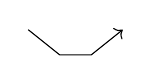
\begin{tikzpicture}[scale=0.4]
		\draw[->] (0, 0.8) -- (1, 0) -- (2, 0) -- (3, 0.8);
	\end{tikzpicture}
	tidak bergantung pada struktur penjumlahan pada himpunan-himpunan $\Hom$.
	Komposisi itu hanya melibatkan produk hingga dan koproduk hingga dalam
	kategori, termasuk kasus khususnya berupa objek nol, serta
	morfisme-morfisme kanonik yang terkait dengannya.

	Untuk (iii), ingat bahwa semua produk hingga (atau koproduk hingga) dapat
	dibentuk dari objek nol dan biproduk $\oplus$.

	Jika $(F,G)$ merupakan pasangan adjoin, maka $F$ mempertahankan
	$\varinjlim$, sedangkan $G$ mempertahankan $\varprojlim$; lihat
	\cite[Teorema 2.8.12]{Li1}. Di sisi lain, ekuivalensi mempertahankan semua
	limit. Karena itu, (iv) dan (v) keduanya merupakan kasus khusus dari (ii).
\end{bukti}

% segment-id: o014.li2.chapter1.additive-categories-kernels-cokernels.p010
Sesungguhnya, deskripsi penjumlahan dalam
Proposisi~\ref{prop:additive-cat-addition} menunjukkan bahwa ``keaditifan''
suatu kategori aditif $\mathcal{C}$ merupakan sifat dari kategori
$\mathcal{C}$, bukan struktur tambahan.

% segment-id: o014.li2.chapter1.additive-categories-kernels-cokernels.d002
\begin{definisi}
	\index{kernel (kernel)} \index[sym1]{kerf@$\Ker(f)$}
	\index{kokernel (cokernel)}\index[sym1]{cokerf@$\Coker(f)$}
	Misalkan $\mathcal{C}$ merupakan kategori-$\cate{Ab}$ yang mempunyai objek
	nol, dan $f: X \to Y$ suatu morfisme dalam $\mathcal{C}$.
	% segment-id: o014.li2.chapter1.additive-categories-kernels-cokernels.l006
	\begin{itemize}
		% segment-id: o014.li2.chapter1.additive-categories-kernels-cokernels.i014
		\item Jika penyama $\Ker(f,0)$ ada, maka $\Ker(f):=\Ker(f,0)$ beserta
		$\Ker(f) \hookrightarrow X$ disebut \emph{kernel} dari $f$.
		% segment-id: o014.li2.chapter1.additive-categories-kernels-cokernels.i015
		\item Jika kopenyama $\Coker(f,0)$ ada, maka $\Coker(f):=\Coker(f,0)$
		beserta $Y \twoheadrightarrow \Coker(f)$ disebut \emph{kokernel} dari
		$f$.
	\end{itemize}
	Secara khusus, menurut definisi kedua komposisi $\Ker(f) \to X \to Y$
	dan $X \to Y \to \Coker(f)$ sama dengan $0$.
\end{definisi}

% segment-id: o014.li2.chapter1.additive-categories-kernels-cokernels.p011
Terdapat beberapa sudut pandang yang saling melengkapi mengenai kernel dan
kokernel.
% segment-id: o014.li2.chapter1.additive-categories-kernels-cokernels.l007
\begin{itemize}
	% segment-id: o014.li2.chapter1.additive-categories-kernels-cokernels.i016
	\item Pertama, tinjau $\Ker(f)$. Untuk setiap morfisme $g: T \to X$ dengan
	$fg=0$,\footnote{Catatan penerjemah: teks sumber mengatakan ``untuk setiap
	morfisme'' tanpa mencantumkan syarat $fg=0$ dan, secara dual, $hf=0$.
	Kedua syarat itu dipulihkan di sini karena tepat merupakan hipotesis
	penyama dan kopenyama; lihat koreksi O014-C006.} komposisi
	$T \xrightarrow{g} X \xrightarrow{0} Y$ tentu sama dengan $0$.
	Karena itu, sifat universal $\Ker(f)=\Ker(f,0)$ sebagai penyama dapat
	dinyatakan oleh diagram komutatif
	% segment-id: o014.li2.chapter1.additive-categories-kernels-cokernels.g007
	\[\begin{tikzcd}
		& T \arrow[dashrightarrow, ld, "{\exists! g'}"'] \arrow[d, "g"] \arrow[rd, "0"] & \\
		\Ker(f) \arrow[r] & X \arrow[r, "f"'] & Y .
	\end{tikzcd}\]
	% segment-id: o014.li2.chapter1.additive-categories-kernels-cokernels.i017
	\item Tinjau $\Coker(f)$. Untuk setiap morfisme $h: Y \to T$ dengan
	$hf=0$, komposisi $X \xrightarrow{0} Y \xrightarrow{h} T$ tentu sama dengan
	$0$. Karena itu,
	sifat universal $\Coker(f)=\Coker(f,0)$ sebagai kopenyama dapat dinyatakan
	oleh diagram komutatif
	% segment-id: o014.li2.chapter1.additive-categories-kernels-cokernels.g008
	\[\begin{tikzcd}
		X \arrow[r, "f"] \arrow[rd, "0"'] & Y \arrow[r] \arrow[d, "h"] & \Coker(f) \arrow[dashrightarrow, ld, "{\exists! h'}"] . \\
		& T &
	\end{tikzcd}\]
	% segment-id: o014.li2.chapter1.additive-categories-kernels-cokernels.i018
	\item Kedua konstruksi di atas jelas saling dual:
	$\Coker(f)=\Ker(f^{\opp})$ dan $\Ker(f)=\Coker(f^{\opp})$.
\end{itemize}

% segment-id: o014.li2.chapter1.additive-categories-kernels-cokernels.p012
Karena morfisme yang terfaktorkan melalui objek nol tepat merupakan morfisme
$0$, sifat universal tersebut juga mempunyai karakterisasi melalui diagram
tarik balik dan dorong keluar. Pembaca dipersilakan memverifikasi langsung:

% segment-id: o014.li2.chapter1.additive-categories-kernels-cokernels.g009
\begin{equation}\label{eqn:Ker-Coker-triangles}
	\begin{tikzcd}
		\Ker(f) \arrow[phantom, r, "\simeq" description] & X \dtimes{Y} 0 \arrow[r] \arrow[d] \arrow[phantom, rd, "\Box" description] & X \arrow[d, "f"] \\
		& 0 \arrow[r] & Y
	\end{tikzcd} \qquad \begin{tikzcd}
		X \arrow[r, "f"] \arrow[d] & Y \arrow[d] & \\
		0 \arrow[r] & Y \dsqcup{X} 0 \arrow[phantom, lu, "\boxplus" description] & \Coker(f) \arrow[phantom, l, "\simeq" description] .
\end{tikzcd}\end{equation}

% segment-id: o014.li2.chapter1.additive-categories-kernels-cokernels.r001
\begin{catatan}\label{rem:equalizer-Ker}
	Penyama umum $\Ker(f,g)$ dapat direduksi menjadi kernel di atas. Tinjau
	morfisme-morfisme
	% segment-id: o014.li2.chapter1.additive-categories-kernels-cokernels.g010
	\[\begin{tikzcd}
	T \arrow[r, "h"] & X \arrow[r, yshift=0.2em, "f"] \arrow[r, yshift=-0.2em, "g"'] & Y
	\end{tikzcd}, \]
	Syarat $fh=gh$ ekuivalen dengan $(f-g)h=0$, sehingga langsung diperoleh
	$\Ker(f,g)=\Ker(f-g,0)=:\Ker(f-g)$. Secara dual,
	$\Coker(f,g)=\Coker(f-g,0)=:\Coker(f-g)$.
\end{catatan}

% segment-id: o014.li2.chapter1.additive-categories-kernels-cokernels.p013
Mulai sekarang, kita terutama meninjau kasus ketika $\mathcal{C}$ merupakan
kategori aditif.

% segment-id: o014.li2.chapter1.additive-categories-kernels-cokernels.pr003
\begin{proposisi}\label{prop:Ker-Coker-composite}
	Untuk morfisme-morfisme $X \xrightarrow{f} Y \xrightarrow{g} Z$ dalam
	kategori aditif $\mathcal{C}$, terdapat diagram komutatif
	% segment-id: o014.li2.chapter1.additive-categories-kernels-cokernels.g011
	\[\begin{tikzcd}[row sep=small, column sep=small]
		\Ker(gf) \arrow[rr, "\sim"] \arrow[hookrightarrow, rd] & & X \dtimes{Y} \Ker(g) \arrow[hookrightarrow, ld] \\
		& X &
	\end{tikzcd} \quad \begin{tikzcd}[row sep=small, column sep=small]
		Z \dsqcup{Y} \Coker(f) \arrow[rr, "\sim"] & & \Coker(gf) \\
		& Z \arrow[twoheadrightarrow, lu] \arrow[twoheadrightarrow, ru] &
	\end{tikzcd}\]
	di mana $X \dtimes{Y} \Ker(g) \to X$ (atau
	$Z \to Z \dsqcup{Y} \Coker(f)$) merupakan morfisme kanonik produk serat
	(atau koproduk serat),\footnote{Catatan penerjemah: teks sumber
	menulis ``koproduk'', tetapi objek yang ditampilkan adalah koproduk serat
	$Z \dsqcup{Y} \Coker(f)$ dan bukti berikutnya memakai dualitas terhadap
	produk serat; lihat koreksi O014-C005.} dengan ketentuan bahwa $\Ker$,
	$\Coker$, dan semua limit yang disebutkan ada.
\end{proposisi}

% segment-id: o014.li2.chapter1.additive-categories-kernels-cokernels.pf004
\begin{bukti}
	Berdasarkan \eqref{eqn:Ker-Coker-triangles}, pembentukan produk serat secara
	bertahap memberikan isomorfisme kanonik
	$\Ker(gf) \simeq X \dtimes{Z} 0 \simeq
	X \dtimes{Y} (Y \dtimes{Z} 0) \simeq X \dtimes{Y} \Ker(g)$.
	Dualitas memberikan kasus $\Coker(gf)$.
\end{bukti}

% segment-id: o014.li2.chapter1.additive-categories-kernels-cokernels.p014
Funktorialitas penyama dan kopenyama menginduksi funktorialitas kernel dan
kokernel. Konstruksi ini dicirikan oleh diagram komutatif berikut:

% segment-id: o014.li2.chapter1.additive-categories-kernels-cokernels.g012
\begin{equation}\label{eqn:Ker-Coker-functoriality}\begin{tikzcd}
		\Ker(f) \arrow[r] \arrow[dashrightarrow, d, "\exists!"'] & X \arrow[d, "a"'] \arrow[r, "f"] & Y \arrow[d, "b"] \\
		\Ker(g) \arrow[r] & X' \arrow[r, "g"'] & Y'
	\end{tikzcd} \qquad \begin{tikzcd}
		X \arrow[d, "a"'] \arrow[r, "f"] & Y \arrow[d, "b"] \arrow[r] & \Coker(f) \arrow[dashrightarrow, d, "\exists!"'] \\
		X' \arrow[r, "g"'] & Y' \arrow[r] & \Coker(g) .
\end{tikzcd}\end{equation}

% segment-id: o014.li2.chapter1.additive-categories-kernels-cokernels.p015
Hasil berikut menunjukkan bahwa tarik balik (atau dorong keluar)
mempertahankan kernel (atau kokernel).

% segment-id: o014.li2.chapter1.additive-categories-kernels-cokernels.pr004
\begin{proposisi}\label{prop:pull-back-ker}
	Jika diagram dalam kategori aditif $\mathcal{C}$
	% segment-id: o014.li2.chapter1.additive-categories-kernels-cokernels.g013
	\[\begin{tikzcd}
		X \arrow[r, "f"] \arrow[d, "a"'] & Y \arrow[d, "b"] \\
		X' \arrow[r, "g"'] & Y'
	\end{tikzcd}\]
	merupakan diagram tarik balik (atau dorong keluar), maka morfisme
	$\Ker(f) \to \Ker(g)$ (atau $\Coker(f) \to \Coker(g)$) dalam
	\eqref{eqn:Ker-Coker-functoriality} merupakan isomorfisme, dengan ketentuan
	bahwa $\Ker$ dan $\Coker$ yang dibicarakan ada.
\end{proposisi}

% segment-id: o014.li2.chapter1.additive-categories-kernels-cokernels.pf005
\begin{bukti}
	Dengan dualitas, cukup dibahas kasus tarik balik. Untuk setiap objek $T$,
	sifat universal memberikan
	% segment-id: o014.li2.chapter1.additive-categories-kernels-cokernels.a001
	\begin{align*}
		\Hom(T, \Ker(f)) & \simeq \Ker\left[ \Hom(T, X) \to \Hom(T, Y) \right] \\
		& \simeq \Ker\left[ \Hom(T, Y) \dtimes{\Hom(T, Y')} \Hom(T, X') \to \Hom(T, Y) \right] \\
		& = \Ker\left[ \Hom(T, X') \to \Hom(T, Y') \right] \simeq \Hom(T, \Ker(g)),
	\end{align*}
	dengan setiap panah bersifat kanonik. Lema Yoneda kemudian memberikan
	$\Ker(f) \rightiso \Ker(g)$; lihat tinjauan dalam
	Teorema~\sourcecrossref{prop:Yoneda}{A.1.1}.
\end{bukti}

% segment-id: o014.li2.chapter1.additive-categories-kernels-cokernels.lm001
\begin{lema}\label{prop:mono-epi-ker-coker}
	Misalkan $\mathcal{C}$ merupakan kategori aditif dan $f: X \to Y$ suatu
	morfisme dalam $\mathcal{C}$. Maka:
	% segment-id: o014.li2.chapter1.additive-categories-kernels-cokernels.l008
	\begin{enumerate}[(i)]
		% segment-id: o014.li2.chapter1.additive-categories-kernels-cokernels.i019
		\item $f$ merupakan monomorfisme (atau epimorfisme) jika dan hanya jika
		$\Ker(f)=0$ (atau $\Coker(f)=0$);
		% segment-id: o014.li2.chapter1.additive-categories-kernels-cokernels.i020
		\item $f$ merupakan morfisme nol jika dan hanya jika
		$\Ker(f) \rightiso X$, dan ini juga ekuivalen dengan
		$Y \rightiso \Coker(f)$;
		% segment-id: o014.li2.chapter1.additive-categories-kernels-cokernels.i021
		\item Diberikan $k: Y \to Z$ (atau $k': W \to X$), terdapat secara unik
		diagram komutatif berikut:
		% segment-id: o014.li2.chapter1.additive-categories-kernels-cokernels.g014
		\[\begin{tikzcd}[row sep=small, column sep=small]
		\Ker(kf) \arrow[rd] & & \Ker(f) \arrow[ld] \arrow[hookrightarrow, ll, "\exists !"'] \\
		& X &
		\end{tikzcd} \quad \text{atau} \quad
		\begin{tikzcd}[row sep=small, column sep=small]
		\Coker(fk') \arrow[twoheadrightarrow, rr, "\exists !"] & & \Coker(f) \\
		& Y \arrow[lu] \arrow[ru] &
		\end{tikzcd}\]
		dengan ketentuan bahwa kernel (atau kokernel) yang dibicarakan ada. Jika
		$k$ merupakan monomorfisme (atau $k'$ merupakan epimorfisme), maka
		$\Ker(f) \rightiso \Ker(kf)$ (atau
		$\Coker(fk') \rightiso \Coker(f)$).
	\end{enumerate}
\end{lema}

% segment-id: o014.li2.chapter1.additive-categories-kernels-cokernels.pf006
\begin{bukti}
	Pertama, tinjau (i). Berdasarkan dualitas, cukup dibahas kasus
	monomorfisme. Menurut definisi, $f$ merupakan monomorfisme jika dan hanya
	jika untuk setiap pasangan morfisme $g_1,g_2: T \to X$ berlaku
	$f(g_1-g_2)=0 \iff g_1-g_2=0$. Ini setara dengan pernyataan bahwa untuk
	setiap $g: T \to X$, berlaku $fg=0$ jika dan hanya jika $g$ terfaktorkan
	sebagai $T \to 0 \to X$. Pernyataan terakhir ini tepat menyatakan bahwa
	objek nol memenuhi sifat universal $\Ker(f)$.

	Untuk (ii), secara serupa cukup dibuktikan
	$f=0 \iff \Ker(f) \rightiso X$. Akan tetapi,
	$\Ker(f)=\Ker(f,0)$, sehingga ekuivalensi yang diinginkan langsung
	mengikuti definisi penyama.

	Untuk (iii), sekali lagi cukup ditinjau kasus $\Ker$:
	% segment-id: o014.li2.chapter1.additive-categories-kernels-cokernels.g015
	\[\begin{tikzcd}[column sep=small]
		\left\{ g \in \Hom(T, X): fg=0 \right\} \arrow[phantom, r, "\subset" description] & \left\{ g \in \Hom(T, X): kfg=0 \right\} \\
		\Hom(T, \Ker(f)) \arrow[u, "1:1"] & \Hom(T, \Ker(kf)) \arrow[u, "1:1"']
	\end{tikzcd}\]
	Jika $k$ merupakan monomorfisme, inklusi pada baris pertama merupakan
	kesamaan. Terapkan Lema Yoneda untuk menyelesaikan pembuktian.
\end{bukti}

% segment-id: o014.li2.chapter1.additive-categories-kernels-cokernels.p016
Dalam kategori aditif, citra dan kocitra yang diperkenalkan dalam
Definisi~\ref{def:Im-Coim} mempunyai deskripsi sederhana.

% segment-id: o014.li2.chapter1.additive-categories-kernels-cokernels.pr005
\begin{proposisi}\label{prop:Im-Coim-additive}
	\index{citra (image)}\index{kocitra (coimage)}
	\index[sym1]{imf@$\Image(f)$}\index[sym1]{coimf@$\Coim(f)$}
	Misalkan $f: X \to Y$ merupakan morfisme dalam kategori aditif
	$\mathcal{C}$. Maka terdapat isomorfisme kanonik
	% segment-id: o014.li2.chapter1.additive-categories-kernels-cokernels.a002
	\begin{align*}
		\Image(f) & \simeq \Ker\left[ Y \to \Coker(f) \right] \hookrightarrow Y, \\
		\Coim(f) & \simeq \Coker\left[ \Ker(f) \to X \right] \twoheadleftarrow X ;
	\end{align*}
	dengan ketentuan bahwa kernel dan kokernel yang dibicarakan ada.
\end{proposisi}

% segment-id: o014.li2.chapter1.additive-categories-kernels-cokernels.pf007
\begin{bukti}
	Berdasarkan dualitas, cukup ditinjau $\Image(f)$. Ambil morfisme kanonik
	$i_1,i_2: Y \to Y \dsqcup{X} Y$. Dengan menerapkan Lema Yoneda, cukup
	dibuktikan, untuk setiap $T \in \Obj(\mathcal{C})$, bahwa
	% segment-id: o014.li2.chapter1.additive-categories-kernels-cokernels.q008
	\begin{multline*}
		\Hom\left( T, \Image(f) \right) = \left\{ h: T \to Y \;\middle|\; i_1 h = i_2 h \right\} \\
		= \left\{ \begin{array}{r|l}
			h: T \to Y & \forall S \in \Obj(\mathcal{C}),\; \forall s_1, s_2: Y \to S, \\
			& s_1 f = s_2 f \implies s_1 h = s_2 h
		\end{array}\right\} \\
		\xlongequal{s := s_1 - s_2} \left\{ \begin{array}{r|l}
			h: T \to Y & \forall S \in \Obj(\mathcal{C}),\; \forall s: Y \to S, \\
			& s f = 0 \implies sh = 0
		\end{array}\right\} \\
		= \left\{ \begin{array}{r|l}
			h: T \to Y & T \xrightarrow{h} Y \twoheadrightarrow \Coker(f) \\
			& \text{komposisinya adalah}\; 0
		\end{array}\right\}
		\leftiso \Hom\left( T, \Ker\left[ Y \to \Coker(f) \right] \right).
	\end{multline*}
	Kesamaan pertama di atas berasal dari
	$\Image(f):=\Ker(i_1,i_2)$. Untuk kesamaan kedua, mula-mula tuliskan ulang
	syarat pada $h$ sebagai $s'i_1h=s'i_2h$ bagi setiap
	$s': Y \dsqcup{X} Y \to S$, lalu gunakan sifat universal koproduk serat
	% segment-id: o014.li2.chapter1.additive-categories-kernels-cokernels.a003
	\begin{align*}
		\Hom\left( Y \dsqcup{X} Y, S \right) & \xrightarrow{1:1} \Hom(Y,S) \dtimes{\Hom(X,S)} \Hom(Y,S) \\
		s' & \longmapsto \left( s' i_1, s' i_2 \right) =: (s_1, s_2).
	\end{align*}
	Kesamaan keempat diperoleh dari sifat universal kokernel, sehingga cukup
	diambil $S=\Coker(f)$.
\end{bukti}

% segment-id: o014.li2.chapter1.additive-categories-kernels-cokernels.p017
Contoh paling sederhana terjadi ketika $f$ merupakan morfisme nol. Dalam hal
ini, Lema~\ref{prop:mono-epi-ker-coker} (ii) memberikan
$\Image(f)=0=\Coim(f)$.

% segment-id: o014.li2.chapter1.additive-categories-kernels-cokernels.e002
\begin{contoh}\label{eg:strict-morphism}
	Sebagai kelanjutan pembahasan pada Contoh~\ref{eg:additive-category},
	pertama-tama kita tinjau kategori $R\dcate{Mod}$. Homomorfisme modul
	$f: A \to B$ selalu mempunyai
	kernel dan kokernel, yang secara klasik diberikan oleh
	$\Ker(f)=f^{-1}(0)$ dan
	$\Coker(f)=B/\{f(a):a \in A\}$. Langsung dari definisi, $\Image(f)$ adalah
	citra $f$ dalam pengertian teori himpunan, sedangkan
	$\Coim(f)=A/\Ker(f)$. Morfisme kanonik
	$\Coim(f) \to \Image(f)$ dalam \eqref{eqn:strict-morphism} tepat
	merupakan isomorfisme kanonik dalam teori modul
	$A/\Ker(f) \rightiso \Image(f)$. Karena itu, semua morfisme dalam
	$R\dcate{Mod}$ bersifat ketat.

	Selanjutnya, tinjau kategori aditif $\cate{Ban}_{\CC}$ dari
	Contoh~\ref{eg:additive-category}. Kernel dari pemetaan linear kontinu
	$f: X \to Y$ adalah $\Ker(f)=f^{-1}(0)$ seperti biasa, dan tetap merupakan
	ruang Banach. Di sisi lain,
	$\Coker(f)=Y/\overline{\left\{f(x):x \in X\right\}}$ dilengkapi dengan
	norma kuosien. Dalam hal ini, morfisme \eqref{eqn:strict-morphism} menjadi
	% segment-id: o014.li2.chapter1.additive-categories-kernels-cokernels.g016
	\[\begin{tikzcd}[row sep=small, column sep=small]
	\Coim(f) \arrow[equal, r] & X/f^{-1}(0) \arrow[r] & \overline{\left\{ f(x): x \in X \right\}} \arrow[equal, r] & \Image(f) \\
	& x + f^{-1}(0) \arrow[mapsto, r] \arrow[phantom, u, "\in" description, sloped] & f(x) \arrow[phantom, u, "\in" description, sloped] &
	\end{tikzcd}\]
	Ruang di sebelah kanan dilengkapi dengan topologi terinduksi dari $Y$,
	sedangkan ruang di sebelah kiri dilengkapi dengan topologi kuosien dari
	$X$. Misalkan
	$f: X \to Y$ merupakan pemetaan linear kontinu dan injektif antara ruang
	Banach, dengan citra padat tetapi tidak surjektif. Dalam keadaan ini,
	$\Coim(f)=X \to Y=\Image(f)$ bukan isomorfisme. Jadi,
	$\cate{Ban}_{\CC}$ mempunyai morfisme yang tidak ketat.
\end{contoh}

% Terjemahan Bahasa Indonesia dari chapter1.tex baris 568--629.
% Sumber: Methods of Algebra, Volume 2, commit
% 9a5803ff77dd3257484cb177f851a73770a59dd3 (CC BY 4.0).
% stable-unit-id: o014.aljabr2.chapter1.linear-categories-over-commutative-rings

% segment-id: o014.li2.chapter1.linear-categories-over-commutative-rings.h001
\section{Perumuman: Kategori Linear atas Gelanggang Komutatif}\label{sec:linear-cat}
\hypertarget{o014.aljabr2.chapter1.linear-categories-over-commutative-rings}{ }

% segment-id: o014.li2.chapter1.linear-categories-over-commutative-rings.p001
Himpunan-himpunan $\Hom$ dalam suatu kategori aditif mempunyai struktur grup
abelian. Dalam banyak situasi, himpunan-himpunan $\Hom$ ini juga dilengkapi
dengan perkalian skalar oleh suatu gelanggang komutatif $\Bbbk$. Sebagai
contoh, dalam $\Bbbk\dcate{Mod}$ setiap himpunan $\Hom$ secara alami merupakan
modul-$\Bbbk$, dan komposisi morfisme bersifat $\Bbbk$-bilinear.

% segment-id: o014.li2.chapter1.linear-categories-over-commutative-rings.d001
\begin{definisi}\label{def:cat-k-linear}
	\index{kategori!$\Bbbk\dcate{Mod}$-}
	\index{linear!$\Bbbk$- ($\Bbbk$-linear)}
	Misalkan $\Bbbk$ merupakan gelanggang komutatif. Andaikan setiap himpunan
	$\Hom$ dalam kategori $\mathcal{A}$ dilengkapi dengan struktur
	modul-$\Bbbk$ sedemikian sehingga komposisi morfisme
	$\Hom(Y, Z) \times \Hom(X, Y) \to \Hom(X, Z)$ merupakan pemetaan
	$\Bbbk$-bilinear untuk semua objek $X,Y,Z$; dengan kata lain, diagram
	berikut komutatif:
	% segment-id: o014.li2.chapter1.linear-categories-over-commutative-rings.g001
	\[\begin{tikzcd}
		\Hom(Y, Z) \times \Hom(X, Y) \arrow[d] \arrow[r, "\text{komposisi}"] & \Hom(X, Z) \\
		\Hom(Y, Z) \dotimes{\Bbbk} \Hom(X, Y) \arrow[ru, bend right, start anchor=east, "{\exists! \; \text{homomorfisme modul-$\Bbbk$}}"']
	\end{tikzcd}  \]
	Dengan data ini, $\mathcal{A}$ disebut \emph{kategori-$\Bbbk\dcate{Mod}$}.

	Misalkan $F: \mathcal{A} \to \mathcal{A}'$ merupakan funktor antara
	kategori-$\Bbbk\dcate{Mod}$. Jika pemetaan
	$\Hom(X,Y) \to \Hom(FX,FY)$ merupakan homomorfisme modul-$\Bbbk$ untuk
	semua $X,Y \in \Obj(\mathcal{A})$, maka $F$ disebut
	\emph{funktor $\Bbbk$-linear}.
\end{definisi}

% segment-id: o014.li2.chapter1.linear-categories-over-commutative-rings.p002
Perhatikan bahwa $\Bbbk\dcate{Mod}$ merupakan kategori monoidal terhadap hasil
kali tensor $\otimes := \dotimes{\Bbbk}$. Oleh karena itu, istilah
``kategori-$\Bbbk\dcate{Mod}$'' konsisten dengan terminologi pengayaan kategori
dalam \cite[\S 3.4]{Li1}. Kategori-$\cate{Ab}$ yang diperkenalkan sebelumnya
tepat merupakan kategori-$\Z\dcate{Mod}$. Sebaliknya, dengan melupakan
perkalian skalar pada suatu kategori-$\Bbbk\dcate{Mod}$, kita memperoleh
kategori-$\cate{Ab}$.

% segment-id: o014.li2.chapter1.linear-categories-over-commutative-rings.e001
\begin{contoh}
	Kategori-$\Bbbk\dcate{Mod}$ yang hanya mempunyai satu objek tepat
	merupakan aljabar-$\Bbbk$. Korespondensinya diberikan oleh
	$\mathcal{A} \mapsto \End_{\mathcal{A}}(\star)$, dengan
	$\Obj(\mathcal{A}) = \{\star\}$.
\end{contoh}

% segment-id: o014.li2.chapter1.linear-categories-over-commutative-rings.p003
Argumen dalam Proposisi~\ref{prop:automatic-Ab-morphism} dapat diterapkan tanpa
perubahan dan memberikan hasil berikut.

% segment-id: o014.li2.chapter1.linear-categories-over-commutative-rings.pr001
\begin{proposisi}\label{prop:automatic-k-morphism}
	Misalkan $\mathcal{A}$ dan $\mathcal{A}'$ merupakan
	kategori-$\Bbbk\dcate{Mod}$.
	% segment-id: o014.li2.chapter1.linear-categories-over-commutative-rings.l001
	\begin{enumerate}
		% segment-id: o014.li2.chapter1.linear-categories-over-commutative-rings.i001
		\item Diberikan sepasang funktor adjoin
		% Diagram adjungsi sumber yang semula sebaris direflow sebagai display
		% terpusat agar tidak menyempitkan atau melampaui lebar baris pembaca.
		% Rantai kesetaraan panjang dalam bukti juga direflow sebagai display.
		% segment-id: o014.li2.chapter1.linear-categories-over-commutative-rings.g002
		\[
		\begin{tikzcd}
			F: \mathcal{A} \arrow[shift left, r] & \mathcal{A}' \arrow[shift left, l] : G
		\end{tikzcd},
		\]
		dengan $F$ dan $G$ keduanya bersifat $\Bbbk$-linear. Maka isomorfisme adjungsi
		$\Hom_{\mathcal{A}'}(F(\cdot),\cdot) \rightiso
		\Hom_{\mathcal{A}}(\cdot,G(\cdot))$ bersifat $\Bbbk$-linear.
		% segment-id: o014.li2.chapter1.linear-categories-over-commutative-rings.i002
		\item Untuk setiap $\alpha: I \to \mathcal{A}$, bijeksi
		% segment-id: o014.li2.chapter1.linear-categories-over-commutative-rings.q001
		\[
			\Hom_{\mathcal{A}}\left(\varinjlim \alpha,T\right)
			\simeq \varprojlim_{i \in \Obj(I)}
			\Hom_{\mathcal{A}}(\alpha(i),T),
			\quad T \in \Obj(\mathcal{A})
		\]
		bersifat $\Bbbk$-linear, asalkan $\varinjlim \alpha$ ada. Pernyataan yang sama
		berlaku untuk $\varprojlim$.
	\end{enumerate}
\end{proposisi}

% segment-id: o014.li2.chapter1.linear-categories-over-commutative-rings.p004
Kecuali dinyatakan lain, mulai sekarang semua funktor dan ekuivalensi antara
kategori-$\Bbbk\dcate{Mod}$ dipahami bersifat $\Bbbk$-linear.

% segment-id: o014.li2.chapter1.linear-categories-over-commutative-rings.d002
\begin{definisi}\label{def:k-linear-cat}
	\index{kategori!$\Bbbk$-linear ($\Bbbk$-linear)}
	Jika suatu kategori aditif $\mathcal{A}$ dilengkapi dengan struktur
	$\Bbbk$-linear yang kompatibel dengan struktur kategori-$\cate{Ab}$ yang
	sudah ada, maka $\mathcal{A}$ beserta data tersebut disebut
	\emph{kategori $\Bbbk$-linear}.
\end{definisi}

% segment-id: o014.li2.chapter1.linear-categories-over-commutative-rings.p005
Hal ini sama artinya dengan mengganti kategori-$\cate{Ab}$ dengan
kategori-$\Bbbk\dcate{Mod}$ dalam pembahasan \S\ref{sec:Ker-Coker}. Sebagian
besar hasil mengenai kategori aditif dalam bab ini dapat diperluas ke situasi
$\Bbbk$-linear dengan argumen yang sama tanpa perubahan. Satu-satunya pengecualian
berkaitan dengan Korolari~\ref{prop:automatic-additivity}: dalam kategori
aditif, penjumlahan pada himpunan $\Hom$ dapat dicirikan oleh sifat kategori itu
sendiri, tetapi hal ini tidak berlaku bagi perkalian skalar oleh $\Bbbk$.
Karena itu, tidak ada alasan bagi funktor (bahkan ekuivalensi) antara kategori
$\Bbbk$-linear untuk otomatis bersifat $\Bbbk$-linear.

% segment-id: o014.li2.chapter1.linear-categories-over-commutative-rings.p006
Berikut ini beberapa hasil mengenai sifat $\Bbbk$-linear. Ingat bahwa
\emph{pusat} suatu kategori $\mathcal{A}$ didefinisikan sebagai
\index{pusat (center)} \index[sym1]{ZA@$Z(\mathcal{A})$}
$Z(\mathcal{A}) := \End(\identity_{\mathcal{A}})$. Unsur-unsurnya merupakan
morfisme dari funktor identitas $\identity_{\mathcal{A}}$ ke dirinya sendiri,
yang ditulis sebagai $(a_X)_{X \in \Obj(\mathcal{A})}$ dengan
$a_X \in \End_{\mathcal{A}}(X)$. Dengan operasi komposisi morfisme, pusat tersebut
merupakan monoid komutatif; lihat \cite[Definisi 2.3.8,
Proposisi 2.3.9]{Li1}. Jika $\mathcal{A}$ merupakan kategori-$\cate{Ab}$, maka
$Z(\mathcal{A})$ menjadi gelanggang komutatif terhadap komposisi dan
penjumlahan
$(a_X)_X + (b_X)_X := (a_X+b_X)_X$.

% segment-id: o014.li2.chapter1.linear-categories-over-commutative-rings.pr002
\begin{proposisi}\label{prop:k-linear-center}
	Misalkan $\mathcal{A}$ merupakan kategori-$\cate{Ab}$. Maka terdapat
	bijeksi
	% segment-id: o014.li2.chapter1.linear-categories-over-commutative-rings.q002
	\[
		\left\{\text{struktur kategori-$\Bbbk\dcate{Mod}$ pada $\mathcal{A}$}\right\}
		\stackrel{1:1}{\longleftrightarrow}
		\Hom_{\text{gelanggang}}(\Bbbk,Z(\mathcal{A})).
	\]
	Pemetaan tersebut diberikan sebagai berikut. Jika struktur
	kategori-$\Bbbk\dcate{Mod}$ pada $\mathcal{A}$ telah ditetapkan, untuk setiap
	$a \in \Bbbk$ dan $X \in \Obj(\mathcal{A})$ definisikan
	$a_X := a \cdot \identity_X \in \End_{\mathcal{A}}(X)$. Maka
	$a \mapsto (a_X)_{X \in \Obj(\mathcal{A})} \in Z(\mathcal{A})$ merupakan
	homomorfisme gelanggang. Sebaliknya, diberikan homomorfisme gelanggang di
	ruas kanan,
	$a \mapsto (a_X)_{X \in \Obj(\mathcal{A})}$, definisikan struktur
	kategori-$\Bbbk\dcate{Mod}$ pada $\mathcal{A}$ dengan
	$a \cdot f := f \circ a_X = a_Y \circ f$, untuk
	$f \in \Hom(X,Y)$.
\end{proposisi}

% segment-id: o014.li2.chapter1.linear-categories-over-commutative-rings.pf001
\begin{bukti}
	Syarat yang mencirikan
	$(a_X)_{X \in \Obj(\mathcal{A})} \in Z(\mathcal{A})$ adalah
	$f \circ a_X = a_Y \circ f$ untuk setiap $f \in \Hom(X,Y)$. Jika
	$\mathcal{A}$ dilengkapi dengan struktur kategori-$\Bbbk\dcate{Mod}$,
	definisikan $a_X := a \cdot \identity_X$. Sifat bilinear memberikan
	\[
		f \circ a_X = f \circ (a \cdot \identity_X)
		= (a f) \circ \identity_X
		= (a \cdot \identity_Y) \circ f
		= a_Y \circ f,
	\]
	sehingga $(a_X)_{X \in \Obj(\mathcal{A})} \in Z(\mathcal{A})$.
	Verifikasi lainnya langsung.
\end{bukti}

% segment-id: o014.li2.chapter1.linear-categories-over-commutative-rings.p007
Sebagai akibatnya, kategori-$\cate{Ab}$ $\mathcal{A}$ secara alami menjadi
kategori-$Z(\mathcal{A})\dcate{Mod}$.

% Terjemahan lengkap Bahasa Indonesia dari chapter1.tex baris 630--762.
% Sumber: Methods of Algebra, Volume 2, commit
% 9a5803ff77dd3257484cb177f851a73770a59dd3 (CC BY 4.0).
% stable-unit-id: o014.aljabr2.chapter1.limits-through-functors

% segment-id: o014.li2.chapter1.limits-through-functors.h001
\section{Meninjau Limit melalui Funktor}\label{sec:limit-functor}
\hypertarget{o014.aljabr2.chapter1.limits-through-functors}{ }

% segment-id: o014.li2.chapter1.limits-through-functors.p001
Berbagai hubungan antara funktor $F: \mathcal{C} \to \mathcal{D}$ dan limit
secara garis besar dapat dibagi ke dalam dua arah. Ambil $\varinjlim$ sebagai
contoh. Diberikan funktor $\alpha: I \to \mathcal{C}$, pertanyaannya adalah:
% segment-id: o014.li2.chapter1.limits-through-functors.l001
\begin{itemize}
	% segment-id: o014.li2.chapter1.limits-through-functors.i001
	\item Andaikan $\varinjlim \alpha$ ada. Apakah citra
	$F\left(\varinjlim \alpha\right)$ memberikan $\varinjlim (F\alpha)$?
	% segment-id: o014.li2.chapter1.limits-through-functors.i002
	\item Andaikan $\varinjlim F\alpha$ ada. Dapatkah limit itu
	``diangkat'' ke $\mathcal{C}$? Dalam arti apa pengangkatan tersebut unik?
\end{itemize}

% segment-id: o014.li2.chapter1.limits-through-functors.p002
Di sini kita terutama membahas kasus $\varinjlim$. Hasil-hasil ini tentu juga
mempunyai versi yang bersesuaian untuk $\varprojlim$; berkat dualitas,
rinciannya tidak perlu diulang.

% segment-id: o014.li2.chapter1.limits-through-functors.p003
Kita akan menata pembahasan $\varinjlim$ dengan bahasa kokonus dan kategori
$(\alpha/\Delta)$.

% segment-id: o014.li2.chapter1.limits-through-functors.c001
\begin{konvensi}\label{con:limit-cone}
	Untuk funktor $\alpha: I \to \mathcal{C}$ yang telah ditetapkan, data
	$(L, (f_i)_{i \in \Obj(I)})$ di $\mathcal{C}$ yang memenuhi syarat-syarat
	berikut disebut \emph{kokonus} dengan alas $\alpha$ dan puncak $L$:
	% segment-id: o014.li2.chapter1.limits-through-functors.l002
	\begin{compactitem}
		% segment-id: o014.li2.chapter1.limits-through-functors.i003
		\item $L$ merupakan objek di $\mathcal{C}$,
		% segment-id: o014.li2.chapter1.limits-through-functors.i004
		\item setiap $f_i : \alpha(i) \to L$ merupakan morfisme di
		$\mathcal{C}$ dan memenuhi syarat kompatibilitas
		$f_j \circ \alpha(i \to j) = f_i$, dengan $[i \to j]$ berkisar pada
		$\mathrm{Mor}(I)$.
	\end{compactitem}
\end{konvensi}

% segment-id: o014.li2.chapter1.limits-through-functors.p004
Dalam terminologi \cite[\S 2.7]{Li1}, kokonus-kokonus ini membentuk suatu
kategori\footnote{Arti tepat $\Delta$ di sini ialah funktor diagonal
$\mathcal{C} \to \mathcal{C}^I$; lihat Contoh
\sourcecrossref{eg:comma-vs-cone}{1.6.3}. Notasi $\Delta$ dipilih dari huruf
awal pinyin \emph{duìjiǎo} (``diagonal''). Namun, mengikuti asas piktografis,
tidak ada salahnya membayangkan $\Delta$ sebagai ``kokonus''; lihat diagram
\eqref{eqn:injlim-diagram}.} $(\alpha / \Delta)$. Secara konkret, setelah alas
$\alpha$ ditetapkan, suatu morfisme dari kokonus $(L, (f_i)_i)$ ke kokonus
$(M, (g_i)_i)$ ialah diagram komutatif
% segment-id: o014.li2.chapter1.limits-through-functors.g001
\begin{equation}\label{eqn:injlim-diagram}\begin{tikzcd}
	& L \arrow[d] & \\
	\alpha(i) \arrow[bend right, rr, "\alpha(i \to j)"'] \arrow[r, "g_i"] \arrow[ru, "f_i"] & M & \alpha(j) \arrow[l, "{g_j}"'] \arrow[lu, "f_j"']
\end{tikzcd}\end{equation}
dengan $i \to j$ berkisar pada $\Mor(I)$; komposisi morfisme didefinisikan
dengan cara yang jelas. Menurut definisi, $\varinjlim \alpha$ beserta keluarga
morfisme kanonik bawaannya
$\iota_i: \alpha(i) \to \varinjlim \alpha$ merupakan objek awal dari
$(\alpha / \Delta)$.
\index{limit}\index[sym1]{lim}

% segment-id: o014.li2.chapter1.limits-through-functors.p005
Funktor $F$ secara langsung menginduksi funktor
$(\alpha/\Delta) \to (F\alpha / \Delta)$, yang memetakan kokonus
$(L, (f_i)_i)$ ke $(FL, (Ff_i)_i)$. Andaikan $\varinjlim \alpha$ ada. Jika
$\varinjlim F\alpha$ juga ada, maka dalam $(F\alpha / \Delta)$ terdapat
morfisme tunggal
% segment-id: o014.li2.chapter1.limits-through-functors.q001
\[ \varinjlim F\alpha \to F(\varinjlim \alpha), \]
dan morfisme ini merupakan isomorfisme jika dan hanya jika
$\left( F(\varinjlim \alpha), (F\iota_i)_i \right)$ memberikan
$\varinjlim F\alpha$.

% segment-id: o014.li2.chapter1.limits-through-functors.p006
Dengan membalik panah-panah, $\varprojlim \alpha$ dapat dicirikan sebagai
objek terminal dari $(\Delta/\alpha)$. Dengan asumsi bahwa kedua limit
projektif yang dibahas ada, dalam $(\Delta/F\alpha)$ terdapat morfisme tunggal
% segment-id: o014.li2.chapter1.limits-through-functors.q002
\[ F\varprojlim \alpha \to \varprojlim F\alpha. \]

% segment-id: o014.li2.chapter1.limits-through-functors.d001
\begin{definisi}\label{def:create-limit}
	\index{limit!mempertahankan, merefleksikan, menciptakan (preserve, reflect, create)}
	Diberikan $F: \mathcal{C} \to \mathcal{D}$ dan funktor
	$\alpha: I \to \mathcal{C}$, tinjau funktor di antara kategori kokonus
	$(\alpha/\Delta) \to (F\alpha/\Delta)$.
	% segment-id: o014.li2.chapter1.limits-through-functors.l003
	\begin{itemize}
		% segment-id: o014.li2.chapter1.limits-through-functors.i005
		\item Funktor $F$ dikatakan \emph{mempertahankan} $\varinjlim$ ini jika
		$(\alpha/\Delta) \to (F\alpha/\Delta)$ memetakan objek awal (jika ada)
		ke objek awal.
		% segment-id: o014.li2.chapter1.limits-through-functors.i006
		\item Funktor $F$ dikatakan \emph{merefleksikan} $\varinjlim$ ini jika,
		apabila suatu objek dari $(\alpha/\Delta)$ dipetakan menjadi objek awal
		dari $(F\alpha/\Delta)$, objek itu sendiri merupakan objek awal.
		% segment-id: o014.li2.chapter1.limits-through-functors.i007
		\item Funktor $F$ dikatakan \emph{menciptakan} $\varinjlim$ ini jika,
		begitu $\varinjlim F\alpha$ ada, $\varinjlim \alpha$ juga ada, dan dalam
		keadaan ini $F$ mempertahankan $\varinjlim$ tersebut dan juga
		merefleksikan $\varinjlim$ tersebut.
	\end{itemize}
	Untuk $\varprojlim$ terdapat konsep-konsep yang bersesuaian. Konsep-konsep
	untuk $\varinjlim$ dan $\varprojlim$ ini dapat saling diperoleh dengan
	mengganti $\mathcal{C}$ dan $\mathcal{D}$ oleh
	$\mathcal{C}^{\opp}$ dan $\mathcal{D}^{\opp}$.
\end{definisi}

% segment-id: o014.li2.chapter1.limits-through-functors.p007
Perhatikan bahwa konsep-konsep ini bergantung pada $\alpha$ yang sedang
dibahas. Sebagai contoh, sangat mungkin $F$ mempertahankan semua
$\varinjlim$ berhingga tetapi tidak mempertahankan $\varinjlim$ secara umum.

% segment-id: o014.li2.chapter1.limits-through-functors.p008
Untuk $\alpha$ tertentu, pernyataan bahwa suatu funktor menciptakan
$\varinjlim$ (atau $\varprojlim$) setara dengan mengatakan bahwa kokonus (atau
konus) di $\mathcal{D}$ yang mendefinisikan limit tersebut dapat diangkat
secara unik ke $\mathcal{C}$, dan hasil pengangkatan itu memberikan limit yang
bersesuaian di $\mathcal{C}$. Keunikan tersebut berasal dari syarat dalam
definisi mengenai merefleksikan $\varinjlim$ (atau $\varprojlim$). Sudut
pandang ini akan tampak jelas dalam Contoh \ref{eg:Grp-Set-create} dan
Proposisi \ref{prop:forget-create} di bawah.

% segment-id: o014.li2.chapter1.limits-through-functors.pr001
\begin{proposisi}\label{prop:ff-reflect}
	Setiap funktor penuh dan setia merefleksikan semua $\varinjlim$ dan
	$\varprojlim$.
\end{proposisi}
% segment-id: o014.li2.chapter1.limits-through-functors.pf001
\begin{bukti}
	Cukup tinjau $\varinjlim$. Jika $F$ penuh dan setia, sifat universal objek
	awal dari $(\alpha/\Delta)$ dapat diverifikasi di $(F\alpha/\Delta)$ setelah
	menerapkan $F$.
\end{bukti}

% segment-id: o014.li2.chapter1.limits-through-functors.p009
Sejalan dengan pembahasan ini, kita perkenalkan sebuah konsep yang berguna.

% segment-id: o014.li2.chapter1.limits-through-functors.d002
\begin{definisi}\label{def:conservative}
	\index{funktor!konservatif (conservative)}
	Funktor $F$ yang memenuhi syarat berikut disebut \emph{konservatif}:
	morfisme $f \in \Mor(\mathcal{C})$ merupakan isomorfisme jika dan hanya jika
	$Ff \in \Mor(\mathcal{D})$ merupakan isomorfisme.
\end{definisi}

% segment-id: o014.li2.chapter1.limits-through-functors.r001
\begin{catatan}\label{rem:conservative-reflect}
	Jika $F$ merupakan funktor konservatif, maka asalkan
	$\varinjlim \alpha$ ada dan $F$ mempertahankan $\varinjlim$ ini, $F$ juga
	harus merefleksikan $\varinjlim$ ini. Alasannya sebagai berikut. Misalkan
	$L \in \Obj((\alpha/\Delta))$ dipetakan menjadi objek awal dari
	$(F\alpha/\Delta)$. Tinjau morfisme tunggal
	$\varinjlim \alpha \to L$ dalam $(\alpha/\Delta)$. Karena $F$
	mempertahankan $\varinjlim$ ini, citra morfisme tersebut di bawah $F$
	harus merupakan isomorfisme. Syarat konservatif kemudian memastikan bahwa
	$\varinjlim \alpha \to L$ juga merupakan isomorfisme.

	Dengan hipotesis ini, syarat merefleksikan $\varinjlim$ dapat dihapus dari
	definisi bahwa $F$ menciptakan $\varinjlim$.
\end{catatan}

% segment-id: o014.li2.chapter1.limits-through-functors.e001
\begin{contoh}\label{eg:Grp-Set-create}
	Kita akan memverifikasi bahwa funktor pelupa $U$ dari kategori grup
	$\cate{Grp}$ ke kategori himpunan $\cate{Set}$ menciptakan semua
	$\varprojlim$ kecil.

	Hal ini merupakan akibat konstruksi konkret $\varprojlim$ dalam
	$\cate{Grp}$ dan $\cate{Set}$; lihat
	\cite[Contoh 2.7.5 dan 2.8.7]{Li1}. Secara lebih terperinci, ambil kategori
	kecil $I$ dan funktor $\beta: I^{\opp} \to \cate{Grp}$. Sebagai himpunan,
	% segment-id: o014.li2.chapter1.limits-through-functors.q003
	\[ \varprojlim U\beta = \left\{\begin{array}{r|l}
		(x_i)_i \in \prod_{i \in \Obj(I)} U\beta(i) & \forall [i \to j] \in \mathrm{Mor}(I), \\
		& \beta(i \to j)(x_j) = x_i
	\end{array}\right\}, \]
	dan proyeksi $p_i: \varprojlim U\beta \to U\beta(i)$ memetakan $(x_j)_j$
	ke $x_i$. Tugas kita sekarang adalah:
	% segment-id: o014.li2.chapter1.limits-through-functors.l004
	\begin{enumerate}
		% segment-id: o014.li2.chapter1.limits-through-functors.i008
		\item melengkapi $\varprojlim U\beta$ dengan struktur grup sedemikian
		hingga setiap $p_i$ merupakan homomorfisme grup, serta menunjukkan bahwa
		struktur grup semacam itu unik;
		% segment-id: o014.li2.chapter1.limits-through-functors.i009
		\item memverifikasi sifat universal $\varprojlim \beta$ bagi grup ini
		beserta keluarga homomorfisme proyeksi $(p_i)_i$.
	\end{enumerate}

	Jelas bahwa $\varprojlim U\beta$ merupakan subgrup dari hasil kali langsung
	$\prod_i \beta(i)$. Kita notasikan subgrup ini sebagai
	$\varprojlim \beta \in \Obj(\cate{Grp})$; inilah satu-satunya struktur grup
	yang membuat setiap $p_i$ menjadi homomorfisme grup. Dengan demikian, tugas
	pertama selesai.

	Selanjutnya, kita verifikasi sifat universal bagi konus
	$\left( \varprojlim \beta, (p_i)_i\right)$. Tinjau sembarang konus
	$(L, (q_i)_i)$ di $\cate{Grp}$, dengan $q_i: L \to \beta(i)$. Sifat
	universal memberikan pemetaan tunggal
	$\varphi: UL \to \varprojlim U\beta$ sedemikian sehingga
	$p_i \varphi = q_i$ berlaku untuk setiap $i$. Sesungguhnya, $\varphi$ secara konkret
	diberikan oleh $y \mapsto (q_i(y))_{i \in \Obj(I)}$, sehingga pemetaan ini
	merupakan homomorfisme grup $L \to \varprojlim \beta$.\footnote{Catatan
	penerjemah: sumber menulis $L \to \varinjlim \beta$; target dikoreksi
	menjadi $L \to \varprojlim \beta$ sesuai limit projektif yang sedang
	dibuktikan (O014-C007).} Verifikasi selesai.
\end{contoh}

% segment-id: o014.li2.chapter1.limits-through-functors.p010
Dengan argumen yang sepenuhnya serupa, dapat ditunjukkan bahwa funktor pelupa
dari kategori ruang Hausdorff kompak $\cate{CHaus}$ ke $\cate{Set}$ juga
menciptakan semua $\varprojlim$ kecil. Verifikasi terkait diserahkan sebagai
latihan dalam bab ini.

% segment-id: o014.li2.chapter1.limits-through-functors.p011
Hasil berikutnya melibatkan kategori funktor berbentuk $\mathcal{C}^J$
(yang mungkin merupakan kategori ``besar'', tetapi ini tidak menjadi masalah).
Kita memerlukan dua langkah persiapan.

% segment-id: o014.li2.chapter1.limits-through-functors.l005
\begin{itemize}
	% segment-id: o014.li2.chapter1.limits-through-functors.i010
	\item Misalkan $J$ merupakan himpunan. Hasil kali $J$ salinan
	$\mathcal{C}$, yakni $\mathcal{C}^J$, didefinisikan sebagai
	$\Obj\left(\mathcal{C}^J\right) = \Obj(\mathcal{C})^J$ dan
	$\mathrm{Mor}\left(\mathcal{C}^J \right) = \mathrm{Mor}(\mathcal{C})^J$.
	Untuk setiap $j \in J$ terdapat funktor proyeksi yang jelas
	$p_j: \mathcal{C}^J \to \mathcal{C}$.

	% Koreksi O014-C008: sumber menggandakan aksara pada frasa "untuk setiap".
	Diberikan kategori $I$ dan funktor $\alpha: I \to \mathcal{C}^J$, jika
	$\varinjlim (p_j \alpha)$ ada untuk setiap $j$, maka
	$\varinjlim \alpha$ juga ada. Konstruksinya dilakukan dengan mengambil limit
	secara ``titik demi titik'' atau ``objek demi objek'':
	$\varinjlim \alpha = \left( \varinjlim (p_j \alpha) \right)_{j \in J}$.

	% segment-id: o014.li2.chapter1.limits-through-functors.i011
	\item Misalkan $J$ merupakan kategori. Kita dapat meninjau kategori funktor
	$\mathcal{C}^J$. Untuk setiap $j \in \Obj(J)$ terdapat funktor evaluasi
	$\mathrm{ev}_j: \mathcal{C}^J \to \mathcal{C}$, yang memetakan objek $F$
	ke $Fj$ dan memetakan morfisme
	$\varphi = (\varphi_{j'})_{j' \in \Obj(J)}$ ke $\varphi_j$. Nanti kita akan
	meninjau funktor berbentuk $\alpha: I \to \mathcal{C}^J$ beserta
	$\varinjlim$-nya. Perhatikan bahwa $\alpha$ dapat dipandang sebagai funktor
	$I \times J \to \mathcal{C}$, dengan nilainya ditulis $\alpha(i, j)$.
\end{itemize}

% segment-id: o014.li2.chapter1.limits-through-functors.p012
Kedua sistem notasi tersebut kompatibel. Jika $J$ merupakan kategori diskret
dan dipandang sebagai himpunan, maka $\mathcal{C}^J$ tidak lain adalah hasil
kali yang dibahas sebelumnya. Untuk $J$ umum, funktor pelupa
$\mathcal{F}: \mathcal{C}^J \to \mathcal{C}^{\Obj(J)}$ memetakan objek $F$ ke
$(Fj)_{j \in \Obj(J)}$ dan memetakan morfisme $\varphi$ ke
$(\varphi_j)_{j \in \Obj(J)}$. Karena itu, $\mathrm{ev}_j = p_j \mathcal{F}$.

% segment-id: o014.li2.chapter1.limits-through-functors.pr002
\begin{proposisi}\label{prop:forget-create}
	Misalkan $J$ dan $\mathcal{C}$ merupakan kategori.
	% segment-id: o014.li2.chapter1.limits-through-functors.l006
	\begin{enumerate}[(i)]
		% segment-id: o014.li2.chapter1.limits-through-functors.i012
		\item Funktor pelupa
		$\mathcal{F}: \mathcal{C}^J \to \mathcal{C}^{\Obj(J)}$ menciptakan
		$\varinjlim$ dan $\varprojlim$.
		% segment-id: o014.li2.chapter1.limits-through-functors.i013
		\item Misalkan $I$ merupakan kategori dan setiap funktor
		$I \to \mathcal{C}$ mempunyai $\varinjlim$ (atau $\varprojlim$).
		Maka semua funktor berbentuk $I \to \mathcal{C}^J$ juga mempunyai
		$\varinjlim$ (atau $\varprojlim$) di $\mathcal{C}^J$.
		% segment-id: o014.li2.chapter1.limits-through-functors.i014
		\item Dengan asumsi pada (ii), untuk setiap $j \in \Obj(J)$, funktor
		evaluasi $\mathrm{ev}_j: \mathcal{C}^J \to \mathcal{C}$ mempertahankan
		$\varinjlim$ (atau $\varprojlim$) untuk diagram berbentuk $I$ tersebut.
		Dengan kata lain, limit di $\mathcal{C}^J$ juga didefinisikan
		secara ``titik demi titik'' atau ``objek demi objek''.
	\end{enumerate}
\end{proposisi}
% segment-id: o014.li2.chapter1.limits-through-functors.pf002
\begin{bukti}
	Cukup tinjau kasus $\varinjlim$. Untuk (i), tetapkan
	$\alpha: I \to \mathcal{C}^J$ dan andaikan $\varinjlim \mathcal{F}\alpha$
	ada serta diberikan oleh kokonus
	% segment-id: o014.li2.chapter1.limits-through-functors.q004
	\[ \left( (X(j))_{j \in \Obj(J)}, \; \left( \iota_i = (\iota_{i, j})_{j \in \Obj(J)} \right)_{i \in \Obj(I)} \right) \]
	dengan $\iota_{i,j}: \alpha(i, j) \to X(j)$. Kita ingin mengangkatnya
	menjadi kokonus di $\mathcal{C}^J$ yang memberikan $\varinjlim \alpha$.

	Pertama, perhatikan bahwa
	$X(j) = \varinjlim \alpha(\cdot, j)$ untuk setiap $j$. Untuk setiap morfisme
	$j \to j'$, sifat funktorial limit (lihat
	\cite[Lema 2.7.4]{Li1}) memberikan morfisme tunggal
	$X(j \to j'): X(j) \to X(j')$ yang membuat diagram berikut komutatif:
	% segment-id: o014.li2.chapter1.limits-through-functors.g002
	\[\begin{tikzcd}
		\alpha(i, j) \arrow[r] \arrow[d, "{\iota_{i, j}}"'] & \alpha(i, j') \arrow[d, "{\iota_{i, j'}}"] \\
		X(j) \arrow[r, "{X(j \to j')}"'] & X(j')
	\end{tikzcd} \quad i \in \Obj(I). \]
	Dengan cara ini, $j \mapsto X(j)$ diperluas menjadi funktor
	$X: J \to \mathcal{C}$, sedangkan
	$\iota_i: \alpha(i, \cdot) \to X$ membentuk morfisme di
	$\mathcal{C}^J$. Tidak sulit memverifikasi bahwa
	$(X, (\iota_i)_i) \in \Obj(\alpha/\Delta)$; selanjutnya kita buktikan
	bahwa objek ini merupakan objek awal. Karena funktor $\mathcal{F}$
	konservatif, syarat merefleksikan $\varinjlim$ tidak perlu diverifikasi lagi.

	Diberikan $(L, (f_i)_i) \in \Obj(\alpha/\Delta)$, sifat universal
	$\varinjlim \mathcal{F}\alpha$ menentukan morfisme tunggal
	$\varphi = (\varphi_j)_j : \mathcal{F}X \to \mathcal{F}L$ sedemikian sehingga
	bagian segitiga pada diagram berikut komutatif untuk setiap $(i, j)$:
	% segment-id: o014.li2.chapter1.limits-through-functors.g003
	\[\begin{tikzcd}
		& X(j) \arrow[d, "\varphi_j"] \arrow[r, "{X(j \to j')}" inner sep=0.8em] & X(j') \arrow[d, "\varphi_{j'}"] \\
		\alpha(i, j) \arrow[ru, "{\iota_{i,j}}"] \arrow[r, "f_{i, j}"' inner sep=0.8em] & L(j) \arrow[r, "{L(j \to j')}"' inner sep=0.8em] & L(j')
	\end{tikzcd}\]
	Jika dapat ditunjukkan bahwa bagian persegi komutatif untuk setiap
	$j \to j'$, maka keluarga komponen $\varphi$ membentuk morfisme
	$X \to L$. Bingkai
	luar sudah diketahui komutatif, sehingga
	% segment-id: o014.li2.chapter1.limits-through-functors.q005
	\[ \varphi_{j'} X(j \to j') \iota_{i, j} = L(j \to j') f_{i, j} = L(j \to j') \varphi_j \iota_{i, j} \]
	untuk setiap $i$. Morfisme dengan domain $X(j)$ ditentukan oleh
	komposisinya dengan semua $\iota_{i,j}$, sehingga bagian persegi tersebut
	komutatif.

	Untuk (ii), tinjau funktor $\alpha: I \to \mathcal{C}^J$. Menurut
	pembahasan sebelumnya, $\mathcal{F}\alpha: I \to \mathcal{C}^{\Obj(J)}$
	mempunyai $\varinjlim$, yang didefinisikan secara objek demi objek. Oleh (i),
	$\mathcal{F}$ menciptakan $\varinjlim \alpha$ di $\mathcal{C}^J$,\footnote{Catatan
	penerjemah: teks sumber menulis $\mathcal{C}$ di sini. Targetnya dikoreksi
	menjadi $\mathcal{C}^J$, yaitu domain funktor pelupa $\mathcal{F}$ dan
	kategori yang memuat funktor $X: J \to \mathcal{C}$ yang baru dibangun;
	lihat koreksi O014-C009.}
	sedangkan pernyataan
	pada (iii) bahwa $\mathrm{ev}_j$ mempertahankan $\varinjlim$ tersebut
	merupakan akibat langsung dari konstruksi ini.
\end{bukti}

% Terjemahan Bahasa Indonesia dari chapter1.tex baris 763--925.
% Sumber: Methods of Algebra, Volume 2, commit
% 9a5803ff77dd3257484cb177f851a73770a59dd3 (CC BY 4.0).
% stable-unit-id: o014.aljabr2.chapter1.filtered-inductive-limits

% segment-id: o014.li2.chapter1.filtered-inductive-limits.h001
\section{Limit Induktif Terfilter}\label{sec:filtered-indlim}
\hypertarget{o014.aljabr2.chapter1.filtered-inductive-limits}{ }
\enlargethispage{2\baselineskip}

% segment-id: o014.li2.chapter1.filtered-inductive-limits.p001
Salah satu fakta umum dalam analisis matematika ialah bahwa, jika suatu
barisan konvergen, limitnya dapat dihitung dari subbarisan mana pun. Dalam
teori kategori, gagasan ini diwujudkan oleh konsep kofinalitas. Kita mulai
dari keterhubungan.

% segment-id: o014.li2.chapter1.filtered-inductive-limits.d001
\begin{definisi}\index{kategori!terhubung (connected)}
	Misalkan $I$ suatu kategori. Jika $\Obj(I) \neq \emptyset$ dan, untuk setiap
	$i, i' \in \Obj(I)$, selalu terdapat $n \geq 1$ beserta morfisme-morfisme
	% segment-id: o014.li2.chapter1.filtered-inductive-limits.q001
	\[ i = i_0 \leftarrow i_1 \to i_2 \leftarrow i_3 \to i_4 \leftarrow \cdots \to i_{2n} = i' , \]
	maka $I$ disebut terhubung.
\end{definisi}

% segment-id: o014.li2.chapter1.filtered-inductive-limits.p002
Kita perkenalkan sebuah konsep bantu yang akan digunakan berulang kali dalam
beberapa bagian berikutnya.

% segment-id: o014.li2.chapter1.filtered-inductive-limits.d002
\begin{definisi}[Kategori koma, lihat {\cite[Definisi 2.4.7]{Li1}}]\label{def:comma-category}
	\index{kategori koma (comma category)}
	\index[sym1]{iHHi@$(i/H)$, $(H/i)$}
	\index[sym1]{Pii@$\Pi_{i/}$, $\Pi_{/i}$}
	Diberikan kategori $I$, $J$, dan funktor $H: J \to I$. Misalkan
	$i \in \Obj(I)$.
	% segment-id: o014.li2.chapter1.filtered-inductive-limits.l001
	\begin{itemize}
		% segment-id: o014.li2.chapter1.filtered-inductive-limits.i001
		\item Menurut definisi, objek kategori koma $(i/H)$ (atau $(H/i)$)
		adalah data $(j, i \to Hj)$ (atau $(j, Hj \to i)$), dengan
		$j \in \Obj(J)$ dan $i \to Hj$ (atau $Hj \to i$) merupakan morfisme
		di $I$. Morfisme dari data $(j, i \to Hj)$ ke
		$(j', i \to Hj')$ (atau dari $(j, Hj \to i)$ ke
		$(j', Hj' \to i)$) adalah morfisme $f: j \to j'$ di $J$ yang membuat
		diagram berikut komutatif:
		% segment-id: o014.li2.chapter1.filtered-inductive-limits.g001
		\[\begin{tikzcd}[row sep=small, column sep=small]
			& i \arrow[ld] \arrow[rd] & \\
			Hj \arrow[rr, "{Hf}"'] & & Hj'
		\end{tikzcd} \quad \text{atau} \quad \begin{tikzcd}[row sep=small, column sep=small]
			& i & \\
			Hj \arrow[ru] \arrow[rr, "{Hf}"'] & & Hj' \arrow[lu] .
		\end{tikzcd}\]
		Komposisi dan morfisme identitas didefinisikan sebagaimana biasa.
		% segment-id: o014.li2.chapter1.filtered-inductive-limits.i002
		\item Kedua kategori di atas masing-masing dilengkapi dengan funktor
		proyeksi $\Pi_{i/}: (i/H) \to J$ dan $\Pi_{/i}: (H/i) \to J$, yang
		memetakan objek $(j, i \to Hj)$ (atau $(j, Hj \to i)$) ke $j$ dan
		memetakan morfisme $f$ ke $f$.
		% segment-id: o014.li2.chapter1.filtered-inductive-limits.i003
		\item Setiap morfisme $i \to i'$ di $I$ secara alami menginduksi funktor
		$(i'/H) \to (i/H)$ dan $(H/i) \to (H/i')$, sehingga diagram berikut
		komutatif:
		% segment-id: o014.li2.chapter1.filtered-inductive-limits.g002
		\[\begin{tikzcd}[column sep=small, row sep=small]
			(i'/H) \arrow[rr] \arrow[rd, "{\Pi_{i'/}}"'] & & (i/H) \arrow[ld, "{\Pi_{i/}}"] \\
			& J &
		\end{tikzcd} \quad \begin{tikzcd}[column sep=small, row sep=small]
			(H/i) \arrow[rr] \arrow[rd, "{\Pi_{/i}}"'] & & (H/i') \arrow[ld, "{\Pi_{/i'}}"] . \\
			& J &
		\end{tikzcd}\]
	\end{itemize}
\end{definisi}

% segment-id: o014.li2.chapter1.filtered-inductive-limits.e001
\begin{contoh}\label{eg:comma-vs-cone}
	Tinjau funktor $\alpha: I \to \mathcal{C}$ sebagai objek di
	$\mathcal{C}^I$, dan tinjau pula funktor diagonal
	$\Delta: \mathcal{C} \to \mathcal{C}^I$ yang memetakan setiap objek ke
	funktor konstan yang bersesuaian. Menurut Definisi
	\ref{def:comma-category}, $(\alpha/\Delta)$ tepat merupakan kategori
	``kokonus'' yang diperkenalkan dalam Konvensi \ref{con:limit-cone}, sedangkan
	funktor $\Pi_{\alpha/}$ memetakan setiap kokonus ke puncaknya.
\end{contoh}

% segment-id: o014.li2.chapter1.filtered-inductive-limits.d003
\begin{definisi}\label{def:cofinal} \index{kofinal (cofinal)}
	Untuk funktor $H: J \to I$, jika $(i/H)$ terhubung untuk setiap
	$i \in \Obj(I)$, maka $H$ disebut \emph{kofinal}; jika $H$ merupakan
	funktor inklusi dari suatu subkategori, subkategori $J$ disebut kofinal.
\end{definisi}

% segment-id: o014.li2.chapter1.filtered-inductive-limits.p003
Mudah diverifikasi bahwa jika $I \to J$ dan $J \to K$ keduanya kofinal, maka
funktor komposit $I \to K$ juga kofinal. Pemeriksaannya diserahkan kepada
pembaca sebagai latihan.

% segment-id: o014.li2.chapter1.filtered-inductive-limits.p004
Hasil berikut menunjukkan bahwa limit dapat dihitung dengan membatasi diagram
sepanjang funktor kofinal. Ingat bahwa $H$ menginduksi
$H^{\opp}: J^{\opp} \to I^{\opp}$.

% segment-id: o014.li2.chapter1.filtered-inductive-limits.pr001
\begin{proposisi}\label{prop:cofinal-lim}
	Jika $H: J \to I$ kofinal, maka:
	% segment-id: o014.li2.chapter1.filtered-inductive-limits.l002
	\begin{itemize}
		% segment-id: o014.li2.chapter1.filtered-inductive-limits.i004
		\item untuk funktor $\alpha: I \to \mathcal{C}$ yang diberikan,
		$\varinjlim \alpha$ ada jika dan hanya jika $\varinjlim \alpha H$ ada;
		dalam hal ini terdapat isomorfisme kanonik
		$\varinjlim \alpha H \simeq \varinjlim \alpha$;
		% segment-id: o014.li2.chapter1.filtered-inductive-limits.i005
		\item secara dual, untuk funktor
		$\beta: I^{\opp} \to \mathcal{C}$ yang diberikan,
		$\varprojlim \beta$ ada jika dan hanya jika
		$\varprojlim \beta H^{\opp}$ ada; dalam hal ini terdapat isomorfisme
		kanonik $\varprojlim \beta H^{\opp} \simeq \varprojlim \beta$.
	\end{itemize}
\end{proposisi}
% segment-id: o014.li2.chapter1.filtered-inductive-limits.pf001
\begin{bukti}
	Kita hanya membahas $\varinjlim$. Dalam bahasa
	\S\ref{sec:limit-functor}, cukup dibuktikan bahwa funktor
	$(\alpha/\Delta) \to (\alpha H / \Delta)$ merupakan ekuivalensi; funktor
	ini memetakan kokonus beralas $\alpha$, yakni $(L, (f_i)_i)$, ke kokonus
	beralas $\alpha H$, yakni $(L, (f_{Hj})_j)$.

	Pertama-tama kita buktikan bahwa funktor ini pada hakikatnya surjektif.
	Tinjau $L \in \Obj(\mathcal{C})$ dan keluarga morfisme
	$(g_j: \alpha H(j) \to L)_{j \in \Obj(J)}$ yang memenuhi syarat
	kompatibilitas $g_{j'} \circ \alpha H(j \to j') = g_j$. Untuk setiap
	$i \in \Obj(I)$, karena $(i/H)$ tidak kosong, kita dapat memilih $j$ dan
	$i \to H(j)$. Definisikan
	$f_i := g_j \circ \alpha(i \to H(j))$. Definisi ini tidak bergantung pada
	pilihan objek koma $(j,i \to H(j))$: memang, jika terdapat
	morfisme-morfisme di $(i/H)$ seperti dalam diagram
	% segment-id: o014.li2.chapter1.filtered-inductive-limits.g003
	\[\begin{tikzcd}[column sep=large]
		& i \arrow[ld] \arrow[d] \arrow[rd] & \\
		H(j) & H(j'') \arrow[l, "{H(j'' \to j)}"] \arrow[r, "{H(j'' \to j')}"'] & H(j')
	\end{tikzcd}\]
	maka dari konstruksinya langsung terlihat bahwa
	% segment-id: o014.li2.chapter1.filtered-inductive-limits.q002
	\[ g_j \circ \alpha(i\to H(j))
	= g_{j''} \circ \alpha(i\to H(j''))
	= g_{j'} \circ \alpha(i\to H(j')). \]
	Karena $(i/H)$ terhubung, ini cukup untuk menunjukkan bahwa $f_i$
	terdefinisi dengan baik. Pembahasan di atas juga menyiratkan bahwa
	$(f_i)_i$ memenuhi syarat kompatibilitas
	$f_i=f_{i'}\circ\alpha(i\to i')$: untuk setiap $i \to i'$ dan
	$i' \to H(j')$, kita dapat menghitung $f_i$ menggunakan objek koma
	$(j',i \to i' \to H(j'))$. Jadi,
	$(L, (f_i)_i) \in \Obj((\alpha/\Delta))$ dipetakan ke
	$(L, (g_j)_j)$.

	Selanjutnya kita tunjukkan bahwa funktor ini penuh dan setia. Memberikan
	suatu morfisme di $(\alpha/\Delta)$, yaitu
	$(L, (f_i)_i) \to (L', (f'_i)_i)$, setara dengan memberikan morfisme di
	$\mathcal{C}$, yaitu $\theta: L \to L'$, sedemikian sehingga
	$\theta f_i = f'_i$ selalu berlaku. Cukup memeriksa syarat ini pada
	objek-objek $H(j)$ dalam citra kofinal $H$: untuk setiap $i$, pilih
	$j \in \Obj(J)$ dan $i \to H(j)$; syarat tersebut kemudian menjadi
	$\theta f_{H(j)} = f'_{H(j)}$, yakni bahwa $\theta$ merupakan morfisme di
	$(\alpha H / \Delta)$.
\end{bukti}

% segment-id: o014.li2.chapter1.filtered-inductive-limits.d004
\begin{definisi}
	\index{kategori!terfilter (filtered)}
	\index{limit!terfilter (filtered)}
	Menurut \cite[Definisi 2.7.6]{Li1}, kategori $I$ dengan
	$\Obj(I)\neq\emptyset$ yang memenuhi syarat-syarat berikut disebut
	\emph{terfilter}\footnote{Catatan penerjemah: sumber tidak menyatakan syarat
	$\Obj(I)\neq\emptyset$, sehingga kategori kosong akan memenuhi kedua butir
	secara vakum; sumber juga menyebut $k\in\Obj(I)$ sebagai morfisme pada butir
	kedua. Target menambahkan syarat ketak-kosongan dan memperbaiki jenis $k$
	menjadi objek (O014-C010 dan O014-C011).}.
	% segment-id: o014.li2.chapter1.filtered-inductive-limits.l003
	\begin{compactitem}
		% segment-id: o014.li2.chapter1.filtered-inductive-limits.i006
		\item Untuk setiap $i, j \in \Obj(I)$, terdapat objek $k \in \Obj(I)$
		beserta morfisme $i \rightarrow k$ dan $j \rightarrow k$.
		% segment-id: o014.li2.chapter1.filtered-inductive-limits.i007
		\item Untuk setiap pasangan morfisme $f, g: i \to j$ di $I$, terdapat
		objek $k \in \Obj(I)$ dan morfisme $h: j \to k$ sedemikian sehingga
		$hf = hg$.
	\end{compactitem}

	Jika $I$ merupakan kategori terfilter dan $\alpha: I \to \mathcal{C}$
	merupakan funktor, maka $\varinjlim \alpha$ yang bersesuaian disebut
	\emph{limit induktif terfilter}.
\end{definisi}

% segment-id: o014.li2.chapter1.filtered-inductive-limits.e002
\begin{contoh}\label{eg:filtered-poset}
	\index{himpunan terurut parsial!terfilter (filtered)}
	Salah satu kelas kategori terfilter yang umum berasal dari himpunan
	terurut parsial terfilter\footnote{Ketika digunakan sebagai indeks limit,
	kategori terfilter sering dapat digantikan dengan himpunan terurut parsial
	terfilter; lihat Catatan \sourcecrossref{rem:filtered-poset}{A.2.3} dan
	penjelasan untuk latihan-latihan dalam
	Lampiran~\sourcecrossref{sec:app-Abel}{A}.}. Setiap himpunan terurut parsial
	$(P, \leq)$ menentukan kategori $\mathcal{P}$ yang bersesuaian sedemikian
	sehingga $x \leq y  \iff \Hom_{\mathcal{P}}(x, y) \neq \emptyset$. Jika
	$\mathcal{P}$ merupakan kategori terfilter, maka $(P, \leq)$ disebut
	\emph{himpunan terurut parsial terfilter}. Suatu himpunan terurut parsial
	bersifat terfilter jika dan hanya jika himpunan itu tidak kosong dan setiap
	dua unsurnya $i, j$ mempunyai batas atas bersama $k$. Setiap himpunan
	terurut total yang tidak kosong jelas terfilter.
\end{contoh}

% segment-id: o014.li2.chapter1.filtered-inductive-limits.pr002
\begin{proposisi}\label{prop:cofinal-filtered}
	Misalkan $I$ kategori terfilter. Maka subkategori penuh $J\subset I$
	bersifat kofinal jika dan hanya jika untuk setiap $i \in \Obj(I)$ terdapat
	$j \in \Obj(J)$ dan morfisme $i \to j$; dalam hal ini $J$ juga terfilter.
\end{proposisi}
% segment-id: o014.li2.chapter1.filtered-inductive-limits.pf002
\begin{bukti}
	Arah ``hanya jika'' jelas. Untuk arah ``jika'', diberikan
	$j \leftarrow i \to j'$, dengan $j, j' \in \Obj(J)$, sifat terfilter
	menjamin adanya diagram komutatif
	% segment-id: o014.li2.chapter1.filtered-inductive-limits.g004
	\[\begin{tikzcd}[row sep=tiny, column sep=small]
		& j \arrow[r] & k & j' \arrow[l] & \\
		j \arrow[equal, ru] & & & & j' \arrow[equal, lu] \\
		& & i \arrow[llu] \arrow[uu] \arrow[rru] & &
	\end{tikzcd}\]
	dengan $k \in \Obj(J)$. Ini menunjukkan bahwa $J$ kofinal.

	Untuk membuktikan bahwa $J$ terfilter, ambil sembarang
	$i, j \in \Obj(J)$. Karena $I$
	terfilter, terdapat $k_0 \in \Obj(I)$ beserta morfisme $i\to k_0$ dan
	$j\to k_0$; pilih pula $k \in \Obj(J)$ beserta
	morfisme $k_0 \to k$. Dengan mengomposisikan morfisme-morfisme tersebut,
	di $J$ terdapat morfisme $i \rightarrow k \leftarrow j$.
	\footnote{Catatan penerjemah: sumber menulis
	$i\rightarrow k_0\leftarrow j$ sebagai morfisme-morfisme di $J$, padahal
	$k_0$ hanya diketahui berada di $I$. Target menggunakan komposit menuju
	$k\in\Obj(J)$ (O014-C012).} Ini membuktikan syarat pertama
	untuk kategori terfilter. Syarat kedua dapat dibuktikan dengan gagasan yang
	sama.
\end{bukti}

% segment-id: o014.li2.chapter1.filtered-inductive-limits.e003
\begin{contoh}
	Definisikan
	$\mathrm{OFin}_I := \left\{ \text{subkategori penuh}\; J \subset I: \Obj(J) \;\text{berhingga} \right\}$.
	Himpunan ini, terhadap $\subset$, merupakan himpunan terurut parsial
	terfilter: untuk setiap $J, K \in \mathrm{OFin}_I$, subkategori yang
	diperoleh dengan mengambil gabungan himpunan objeknya merupakan batas atas
	bersama bagi $J$ dan $K$.
\end{contoh}

% segment-id: o014.li2.chapter1.filtered-inductive-limits.p005
Untuk melihat kegunaan konstruksi ini, tinjau sembarang funktor
$\alpha: I \to \mathcal{C}$ (atau $\beta: I^{\opp} \to \mathcal{C}$).
Pembatasannya pada subkategori penuh $J$ memberikan $\alpha|_J$ (atau
$\beta|_{J^{\opp}}$). Jika $J \subset K$, terdapat morfisme alami
$\varinjlim \alpha|_J \to \varinjlim \alpha|_K$ (atau
$\varprojlim \beta|_{K^{\opp}} \to \varprojlim \beta|_{J^{\opp}}$), asalkan
limit-limit tersebut ada. Hasil berikut menjelaskan cara
menghampiri sembarang limit secara ``terfilter'' melalui kasus dengan
objek berhingga.

% segment-id: o014.li2.chapter1.filtered-inductive-limits.pr003
\begin{proposisi}\label{prop:limit-filtered-approx}
	Dalam situasi di atas, terdapat isomorfisme kanonik
	% segment-id: o014.li2.chapter1.filtered-inductive-limits.q003
	\[ \varinjlim_{\substack{J \in \mathrm{OFin}_I \\ \subset}} \varinjlim \alpha|_J \rightiso \varinjlim \alpha \]
	(atau $\varprojlim \beta \rightiso
	\varprojlim_{J \in \mathrm{OFin}_I^{\opp}}
	\varprojlim \beta|_{J^{\opp}}$), dengan syarat limit rangkap pada ruas kiri
	(atau ruas kanan) ada.\footnote{Catatan penerjemah: pada rumus dual, sumber
	menulis limit induktif luar. Namun untuk $J\subset K$, morfisme transisinya
	berarah dari suku $K$ ke suku $J$, sehingga suku-suku itu membentuk diagram
	pada $\mathrm{OFin}_I^{\opp}$ dan konstruksi luarnya adalah limit projektif
	(O014-C013).}
\end{proposisi}
% segment-id: o014.li2.chapter1.filtered-inductive-limits.pf003
\begin{bukti}
	Ambil kasus $\varinjlim$ sebagai contoh. Sifat universal memberikan bijeksi
	kanonik
	% segment-id: o014.li2.chapter1.filtered-inductive-limits.q004
	\[ \begin{aligned}
	\Hom\left( \varinjlim_{J\in\mathrm{OFin}_I} \varinjlim \alpha|_J, S \right)
	&\simeq \varprojlim_{J\in\mathrm{OFin}_I^{\opp}}
	\Hom\left( \varinjlim \alpha|_J, S \right) \\
	&\simeq \varprojlim_{J\in\mathrm{OFin}_I^{\opp}}
	\varprojlim \Hom(\alpha|_J, S) .
	\end{aligned} \]
	dengan $S \in \Obj(\mathcal{C})$ sembarang, sedangkan ruas kanan merupakan
	$\varprojlim$ rangkap dari himpunan. Cukup diperiksa, untuk keluarga
	himpunan $(X_i)_{i \in \Obj(I)}$ beserta keluarga
	morfisme kompatibel
	$\left( f_{i \to j}: X_j \to X_i \right)_{[i \to j] \in \Mor(I)}$,
	bijeksi
	% segment-id: o014.li2.chapter1.filtered-inductive-limits.g005
	\[\begin{tikzcd}[row sep=tiny]
		\displaystyle\varprojlim_{i \in \Obj(I)} X_i \arrow[r, "\sim"] & \displaystyle\varprojlim_{J \in \mathrm{OFin}_I^{\opp}} \displaystyle\varprojlim_{j \in \Obj(J)} X_j \\
		(x_i)_i \arrow[mapsto, r] & \left( (x_j)_{j \in \Obj(J)} \right)_{J \in \mathrm{OFin}_I} .
	\end{tikzcd}\]

	Untuk setiap $J$, konstruksi konkret $\varprojlim$ dari himpunan ialah
	% segment-id: o014.li2.chapter1.filtered-inductive-limits.q005
	\[ \varprojlim_{j \in \Obj(J)} X_j = \left\{ (x_j)_j \in \prod_{j \in \Obj(J)} X_j : \forall [i \to j] \in \Mor(J), \; f_{i \to j}(x_j) = x_i \right\}, \]
	sehingga bijeksi tersebut jelas: setiap data dalam $\varprojlim_i X_i$,
	baik koordinat $x_i$ maupun syarat kompatibilitas
	$f_{i \to j}(x_j) = x_i$, dapat tercakup oleh suatu
	$J \in \mathrm{OFin}_I$.
\end{bukti}

% segment-id: o014.li2.chapter1.filtered-inductive-limits.p006
Ingat bahwa kategori $\cate{Set}$ mempunyai semua $\varinjlim$ dan
$\varprojlim$ kecil. Limit induktif kecil terfilter mempunyai deskripsi yang
sangat baik.

% segment-id: o014.li2.chapter1.filtered-inductive-limits.pr004
\begin{proposisi}\label{prop:filtered-union}
	Misalkan $I$ kategori kecil yang terfilter dan
	$\alpha: I \to \cate{Set}$ funktor. Definisikan relasi biner berikut pada
	himpunan $\bigsqcup_{i \in \Obj(I)} \alpha(i)$: untuk $x \in \alpha(i)$
	dan $y \in \alpha(j)$, relasi $x \sim y$ berarti bahwa terdapat objek
	$k\in\Obj(I)$ beserta morfisme $i\rightarrow k$ dan $j\rightarrow k$
	sedemikian sehingga
	$\alpha(i \to k)(x) = \alpha(j \to k)(y)$. Maka $\sim$ merupakan relasi
	ekuivalensi, dan
	% segment-id: o014.li2.chapter1.filtered-inductive-limits.q006
	\[ \varinjlim \alpha = \left( \bigsqcup_{i \in \Obj(I)} \alpha(i) \right) \big/ \sim . \]
\end{proposisi}
% segment-id: o014.li2.chapter1.filtered-inductive-limits.pf004
\begin{bukti}
	Lihat pembahasan setelah \cite[Definisi 2.7.6]{Li1}.
\end{bukti}

% segment-id: o014.li2.chapter1.filtered-inductive-limits.p007
Selanjutnya, unsur $\varinjlim \alpha$ di atas akan kita tuliskan sebagai
$[x_{i_0}]$, dengan $i_0 \in \Obj(I)$ dan $[x_{i_0}]$ merupakan kelas
ekuivalensi yang memuat $x_{i_0} \in \alpha(i_0)$. Di sisi lain, untuk
kategori kecil umum $J$ dan funktor $\beta: J^{\opp} \to \cate{Set}$, kita
akan menuliskan unsur $\varprojlim \beta$ dalam bentuk
$(y_j)_{j \in \Obj(J)}$, dengan $y_j \in \beta(j)$ memenuhi syarat
kompatibilitas $\beta(j' \to j)(y_j) = y_{j'}$.

% segment-id: o014.li2.chapter1.filtered-inductive-limits.p008
Berikutnya, tinjau funktor berbentuk
$\alpha: I \times J^{\opp} \to \cate{Set}$, dengan $I, J$ kategori kecil;
menurut peubah $I$ dan $J$ masing-masing dapat diambil $\varinjlim$ dan
$\varprojlim$. Untuk setiap $(i_0, j_0) \in \Obj(I \times J)$, terdapat
komposisi pemetaan alami
% segment-id: o014.li2.chapter1.filtered-inductive-limits.q007
\[ \varprojlim_j \alpha(i_0, j) \to \alpha(i_0, j_0) \to \varinjlim_i \alpha(i, j_0); \]
komposisi ini alami dalam $i_0$ dan $j_0$. Dengan memvariasikan $j_0$,
kita memperoleh pemetaan kanonik
$\varprojlim_j \alpha(i_0, j) \to \varprojlim_j \varinjlim_i \alpha(i, j)$;
selanjutnya, dengan memvariasikan $i_0$, kita memperoleh pemetaan kanonik
% segment-id: o014.li2.chapter1.filtered-inductive-limits.q008
\begin{equation}\label{eqn:filtered-finite-exchange}
	e: \varinjlim_i \varprojlim_j \alpha(i, j) \to \varprojlim_j \varinjlim_i \alpha(i, j).
\end{equation}
Dengan menggunakan notasi wakil, $e$ memetakan
$\left[ (x_{i_0, j})_j \right]$ ke
$\left( [ x_{i_0, j}] \right)_j$.

% segment-id: o014.li2.chapter1.filtered-inductive-limits.p009
Jika $\Mor(J)$ merupakan himpunan berhingga, kategori $J$ disebut berhingga;
hal ini setara dengan mensyaratkan bahwa himpunan objeknya dan himpunan
morfisme di antara setiap dua objek semuanya berhingga. Hasil berikut akan
digunakan dalam \S\sourcecrossref{sec:cat-localization}{1.9}.

% segment-id: o014.li2.chapter1.filtered-inductive-limits.pr005
\begin{proposisi}\label{prop:filtered-finite-exchange}
	Misalkan $I$ kategori kecil yang terfilter, $J$ kategori berhingga, dan
	$\alpha: I \times J^{\opp} \to \cate{Set}$ funktor. Maka pemetaan $e$ dalam
	\eqref{eqn:filtered-finite-exchange} merupakan bijeksi.
\end{proposisi}
% segment-id: o014.li2.chapter1.filtered-inductive-limits.pf005
\begin{bukti}
	Pertama-tama kita tunjukkan bahwa $e$ surjektif. Diberikan
	$(b_j)_{j \in \Obj(J)} \in \varprojlim_j \varinjlim_i \alpha(i, j)$,
	tuliskan setiap $b_j$ sebagai $[x_{i_j, j}]$. Karena $I$ terfilter dan $J$
	berhingga, kita dapat memilih objek sasaran bersama $i\in\Obj(I)$ untuk
	semua $i_j$, lalu mengganti setiap wakil dengan citranya sepanjang morfisme
	$i_j\to i$.
	Dengan demikian, semua wakil dapat ditulis $x_{i,j}$ dengan indeks $i$ yang
	sama. Untuk setiap morfisme $j \to j'$ di $J$, kita mempunyai
	% segment-id: o014.li2.chapter1.filtered-inductive-limits.q009
	\[ \left[ \alpha(i, j \to j') (x_{i, j'}) \right] = \left[ x_{i, j} \right]. \]
	Karena $\Mor(J)$ berhingga dan $I$ terfilter, kita dapat memilih satu
	morfisme $i\to i_1$ yang menyamakan semua pasangan tersebut, mengganti
	semua wakil dengan citranya di indeks $i_1$,
	lalu menamai
	kembali $i_1$ sebagai $i$, sehingga
	$\alpha(i, j \to j') (x_{i, j'}) = x_{i, j}$ berlaku untuk semua
	$[j \to j'] \in \Mor(J)$. Karena itu,
	$e\left( [(x_{i, j})_j] \right) = (b_j)_j$.

	Selanjutnya kita tunjukkan bahwa $e$ injektif. Misalkan $e(x) = e(y)$.
	Karena $I$ terfilter, kita dapat mengganti wakil-wakil $x$ dan $y$ dengan
	citranya di satu indeks bersama $i\in\Obj(I)$, sehingga keduanya mempunyai wakil
	$(x_{i,j})_j$ dan $(y_{i,j})_j$. Jadi, untuk setiap $j \in \Obj(J)$,
	berlaku $[x_{i,j}]=[y_{i,j}]$. Karena $I$ terfilter dan $J$ berhingga, kita
	dapat memilih satu indeks lanjutan bersama, mengganti semua komponen dengan
	citranya di sana, lalu menamainya kembali sebagai $i$, sehingga
	$x_{i,j}=y_{i,j}$ untuk setiap
	$j$. Dengan demikian, $x=y$.
\end{bukti}

% Terjemahan Bahasa Indonesia dari chapter1.tex baris 926--1140.
% Sumber: Methods of Algebra, Volume 2, commit
% 9a5803ff77dd3257484cb177f851a73770a59dd3 (CC BY 4.0).
% stable-unit-id: o014.aljabr2.chapter1.kan-extensions

% segment-id: o014.li2.chapter1.kan-extensions.h001
\section{Ekstensi Kan}\label{sec:Kan-extension}
\hypertarget{o014.aljabr2.chapter1.kan-extensions}{ }

% segment-id: o014.li2.chapter1.kan-extensions.p001
Bagian ini bermula dari persoalan memperluas funktor. Tinjau kategori
$\mathcal{C}$, $\mathcal{D}$, $\mathcal{E}$ serta funktor $K$ dan $F$ seperti
dalam diagram berikut:
% segment-id: o014.li2.chapter1.kan-extensions.g001
\[\begin{tikzcd}
	\mathcal{C} \arrow[d, "K"'] \arrow[rd, bend left, "F"] & \\
	\mathcal{D} \arrow[dashed, r, "{\exists ? \; L}"'] & \mathcal{E}
\end{tikzcd}\]
Sesuai dengan semangat dasar teori kategori, kita ingin mencari funktor $L$
yang ditunjukkan oleh garis putus-putus, beserta isomorfisme alami
$F \simeq LK$. Persoalan ini pada umumnya tidak memiliki solusi; misalnya,
mungkin terdapat $f \in \Mor(\mathcal{C})$ sedemikian sehingga $Kf$ merupakan
isomorfisme, sedangkan $Ff$ bukan isomorfisme. Sebagai gantinya, setidaknya
kita dapat bertanya: adakah suatu hampiran terbaik? Jawabannya dicirikan oleh
sifat universal, dalam versi kiri dan kanan.

% segment-id: o014.li2.chapter1.kan-extensions.d001
\begin{definisi}[D.\ Kan]\label{def:Kan-extension}
	\index{ekstensi Kan (Kan extension)}
	\index[sym1]{LanKF@$\Lan_K F$}
	\index[sym1]{RanKF@$\Ran_K F$}
	Tinjau kategori $\mathcal{C}$, $\mathcal{D}$, $\mathcal{E}$, funktor
	$K: \mathcal{C} \to \mathcal{D}$ dan $F: \mathcal{C} \to \mathcal{E}$.
% segment-id: o014.li2.chapter1.kan-extensions.l001
	\begin{itemize}
% segment-id: o014.li2.chapter1.kan-extensions.i001
		\item \emph{Ekstensi Kan kiri} dari funktor $F$ di sepanjang $K$ adalah
		data $(\Lan_K F, \eta)$ berikut:
% segment-id: o014.li2.chapter1.kan-extensions.l002
		\begin{compactitem}
% segment-id: o014.li2.chapter1.kan-extensions.i002
			\item $\Lan_K F: \mathcal{D} \to \mathcal{E}$ merupakan funktor;
% segment-id: o014.li2.chapter1.kan-extensions.i003
			\item $\eta: F \to (\Lan_K F) K$ merupakan transformasi alami.
		\end{compactitem}
		Data ini harus memenuhi sifat universal berikut: untuk setiap data
		$L: \mathcal{D} \to \mathcal{E}$ dan $\xi: F \to LK$, terdapat tepat
		satu transformasi alami $\chi: \Lan_K F \to L$ sedemikian sehingga
		$\xi = (\chi K) \eta$ (komposisi vertikal/horizontal transformasi alami),
		atau, dalam diagram $2$-sel:
% segment-id: o014.li2.chapter1.kan-extensions.g002
		\[\begin{tikzcd}[column sep=large]
			\mathcal{C} \arrow[d, "K"'] \arrow[rd, bend left, "F", ""' {name=F}] & \\
			\mathcal{D} \arrow[r, "L"'] \arrow[Rightarrow, from=F, "\xi" description] & \mathcal{E}
% segment-id: o014.li2.chapter1.kan-extensions.g003
		\end{tikzcd} = \begin{tikzcd}[column sep=large]
			\mathcal{C} \arrow[d, "K"'] \arrow[rd, bend left, "F", ""' {name=F}] & \\
			\mathcal{D} \arrow[r, "{\Lan_K F}"' name=A] \arrow[Rightarrow, from=F, "\eta" description] \arrow[r, "L"{below, name=B}, rounded corners, to path={-- ([yshift=-2em]\tikztostart.south) -- ([yshift=-2em] \tikztotarget.south) [midway]\tikztonodes -- (\tikztotarget) }] & \mathcal{E} \arrow[Rightarrow, from=A, to=B, "\chi"]
		\end{tikzcd}. \]

% segment-id: o014.li2.chapter1.kan-extensions.i004
		\item \emph{Ekstensi Kan kanan} dari funktor $F$ di sepanjang $K$ adalah
		data $(\Ran_K F, \varepsilon)$ berikut:
% segment-id: o014.li2.chapter1.kan-extensions.l003
		\begin{compactitem}
% segment-id: o014.li2.chapter1.kan-extensions.i005
			\item $\Ran_K F: \mathcal{D} \to \mathcal{E}$ merupakan funktor;
% segment-id: o014.li2.chapter1.kan-extensions.i006
			\item $\varepsilon: (\Ran_K  F)K \to F$ merupakan transformasi alami.
		\end{compactitem}
		Data ini harus memenuhi sifat universal berikut: untuk setiap data
		$R: \mathcal{D} \to \mathcal{E}$ dan $\delta: RK \to F$, terdapat tepat
		satu transformasi alami $\theta: R \to \Ran_K F$ sedemikian sehingga
		$\delta = \varepsilon (\theta K)$, atau, dalam diagram $2$-sel:
% segment-id: o014.li2.chapter1.kan-extensions.g004
		\[\begin{tikzcd}[column sep=large]
			\mathcal{C} \arrow[d, "K"'] \arrow[rd, bend left, "F", ""' {name=F}] & \\
			\mathcal{D} \arrow[r, "R"'] \arrow[Rightarrow, to=F, "\delta" description] & \mathcal{E}
% segment-id: o014.li2.chapter1.kan-extensions.g005
		\end{tikzcd} = \begin{tikzcd}[column sep=large]
			\mathcal{C} \arrow[d, "K"'] \arrow[rd, bend left, "F", ""' {name=F}] & \\
			\mathcal{D} \arrow[r, "{\Ran_K F}"' name=A] \arrow[Rightarrow, to=F, "\varepsilon" description] \arrow[r, "R"{below, name=B}, rounded corners, to path={-- ([yshift=-2em]\tikztostart.south) -- ([yshift=-2em] \tikztotarget.south) [midway]\tikztonodes -- (\tikztotarget) }] & \mathcal{E} \arrow[Rightarrow, from=B, to=A, "\theta"]
		\end{tikzcd}. \]
	\end{itemize}
\end{definisi}

% segment-id: o014.li2.chapter1.kan-extensions.p002
Jika dalam definisi tersebut $\mathcal{C}$, $\mathcal{D}$, dan $\mathcal{E}$
diganti masing-masing dengan $\mathcal{C}^{\opp}$, $\mathcal{D}^{\opp}$, dan
$\mathcal{E}^{\opp}$, pola arah funktornya tetap sama, tetapi arah transformasi
alaminya berbalik. Oleh karena itu, ekstensi Kan kiri dan ekstensi Kan kanan
merupakan konsep yang saling dual.

% segment-id: o014.li2.chapter1.kan-extensions.p003
Dengan menggunakan kategori funktor $\mathcal{E}^{\mathcal{C}}$ dan
$\mathcal{E}^{\mathcal{D}}$, sifat universal ekstensi Kan kiri dan kanan
masing-masing menyatakan bijeksi
% segment-id: o014.li2.chapter1.kan-extensions.q001
\begin{equation}\label{eqn:Kan-univ}\begin{aligned}
	\Hom_{\mathcal{E}^{\mathcal{D}}}\left( \Lan_K F, L \right) & \xrightarrow{1:1} \Hom_{\mathcal{E}^{\mathcal{C}}}\left( F, LK \right) \\
	\chi & \longmapsto (\chi K)\eta , \\
	\Hom_{\mathcal{E}^{\mathcal{D}}}\left( R, \Ran_K F \right) & \xrightarrow{1:1} \Hom_{\mathcal{E}^{\mathcal{C}}}\left( RK, F \right) \\
	\theta & \longmapsto \varepsilon (\theta K);
\end{aligned}\end{equation}
inversnya masing-masing adalah pemetaan $(L, \xi) \mapsto \chi$ dan
$(R, \delta) \mapsto \theta$ dari Definisi \ref{def:Kan-extension}.

% segment-id: o014.li2.chapter1.kan-extensions.pr001
\begin{proposisi}\label{prop:Kan-uniqueness}
	Diberikan kategori $\mathcal{C}$, $\mathcal{D}$, $\mathcal{E}$ serta funktor
	$K: \mathcal{C} \to \mathcal{D}$ dan $F: \mathcal{C} \to \mathcal{E}$.
	Perkenalkan funktor tarik balik (yakni, funktor prapengomposisian)
	$K^*: \mathcal{E}^{\mathcal{D}} \to \mathcal{E}^{\mathcal{C}}$ di antara
	kategori-kategori funktor.
% segment-id: o014.li2.chapter1.kan-extensions.l004
	\begin{enumerate}[(i)]
% segment-id: o014.li2.chapter1.kan-extensions.i007
		\item Jika ada, ekstensi Kan kiri $(\Lan_K F, \eta)$ unik hingga
		isomorfisme unik di $\mathcal{E}^{\mathcal{D}}$; hal yang sama berlaku
		untuk ekstensi Kan kanan.
% segment-id: o014.li2.chapter1.kan-extensions.i008
		\item Jika ekstensi Kan kiri (atau ekstensi Kan kanan) di sepanjang $K$
		ada untuk setiap $F$, ekstensi-ekstensi tersebut dapat disusun menjadi
		funktor adjoin kiri bagi $K^*$,
		$\Lan_K: \mathcal{E}^{\mathcal{C}} \to \mathcal{E}^{\mathcal{D}}$
		(atau funktor adjoin kanan
		$\Ran_K: \mathcal{E}^{\mathcal{C}} \to \mathcal{E}^{\mathcal{D}}$);
		keluarga transformasi alami yang tersusun dari $\eta$ (atau
		$\varepsilon$) dalam Definisi \ref{def:Kan-extension} tepat merupakan
		unit (atau kounit) adjungsi tersebut.
	\end{enumerate}
\end{proposisi}
% segment-id: o014.li2.chapter1.kan-extensions.pf001
\begin{bukti}
	Untuk (i), cukup terapkan sifat universal dalam Definisi
	\ref{def:Kan-extension} dengan cara yang lazim.

	Untuk (ii), perhatikan bahwa $LK = K^*(L)$ dan $RK = K^*(R)$; relasi
	adjungsi yang dicari tepat merupakan isi \eqref{eqn:Kan-univ}. Pernyataan
	tentang unit atau kounit diperoleh dengan cara serupa; lihat
	\cite[Proposisi 2.6.5]{Li1}.
\end{bukti}

% segment-id: o014.li2.chapter1.kan-extensions.p004
Menurut konvensi, data $\eta$ atau $\varepsilon$ dalam ekstensi Kan sering kita
hilangkan dari notasi. Jika ekstensi Kan kiri (atau ekstensi Kan kanan) di
sepanjang $K$ ada untuk setiap $F$, funktor $\Lan_K$ (atau $\Ran_K$) yang
diperoleh dari (ii) juga memiliki sifat keunikan yang bersesuaian, berdasarkan
keunikan adjungsi \cite[Proposisi 2.6.10]{Li1}.

% segment-id: o014.li2.chapter1.kan-extensions.r001
\begin{catatan}
	Karena definisi ekstensi Kan hanya melibatkan komposisi $2$-sel, definisi
	tersebut dapat diperluas ke $2$-kategori umum; situasi di sini merupakan
	kasus khusus dalam $2$-kategori $\cate{Cat}$. Lihat
	\cite[\S 3.5]{Li1} untuk perinciannya.
\end{catatan}

% segment-id: o014.li2.chapter1.kan-extensions.p005
Untuk setiap kategori $\mathcal{C}$, tuliskan funktor tunggal
$\mathcal{C} \to \mathbf{1}$ sebagai $!$; menentukan funktor
$\mathbf{1} \to \mathcal{C}$ setara dengan menentukan sebuah objek di
$\mathcal{C}$. Untuk setiap kategori $\mathcal{E}$ dan objeknya $X$, tuliskan
$\Delta(X): \mathcal{C} \to \mathcal{E}$ untuk komposisi
$\mathcal{C} \xrightarrow{!} \mathbf{1} \xrightarrow{\text{konstan}\; X}
\mathcal{E}$; inilah funktor konstan yang memetakan setiap objek ke $X$ dan
setiap morfisme ke $\identity_X$.

% segment-id: o014.li2.chapter1.kan-extensions.e001
\begin{contoh}[Limit sebagai ekstensi Kan]\label{eg:limit-as-Kan}
	Misalkan $F: \mathcal{C} \to \mathcal{E}$ suatu funktor. Tinjau diagram
% segment-id: o014.li2.chapter1.kan-extensions.g006
	\[\begin{tikzcd}
		\mathcal{C} \arrow[d, "!"'] \arrow[rd, bend left, "F"] & \\
		\mathbf{1} & \mathcal{E}
	\end{tikzcd}\]
	Maka $\Lan_! F$ (atau $\Ran_! F$) ada jika dan hanya jika
	$\varinjlim F$ (atau $\varprojlim F$) ada di $\mathcal{E}$, dan dalam hal
	ini ekstensi Kan tersebut tidak lain adalah limit yang bersangkutan.

	Sebagai contoh, tinjau $(\Lan_! F, \eta)$. Funktor
	$\Lan_! F: \mathbf{1} \to \mathcal{E}$ dapat dipandang sebagai objek di
	$\mathcal{E}$, sedangkan $\eta$ merupakan transformasi alami
	$F \to \Delta(\Lan_! F)$ di $\mathcal{E}^{\mathcal{C}}$. Sifat universalnya
	setara dengan pernyataan bahwa data $(\Lan_! F, \eta)$ memberikan objek awal
	dalam kategori $(F/\Delta)$; inilah tepatnya uraian tentang $\varinjlim F$
	dalam \S\ref{sec:limit-functor}.
\end{contoh}

% segment-id: o014.li2.chapter1.kan-extensions.e002
\begin{contoh}[Adjungsi sebagai ekstensi Kan]
	Tinjau sepasang funktor:
% segment-id: o014.li2.chapter1.kan-extensions.g007
	\[\begin{tikzcd}
		F: \mathcal{C} \arrow[r, shift left] & \mathcal{D}: G \arrow[l, shift left]
	\end{tikzcd}\]
	Jika $(F, G)$ dilengkapi menjadi adjungsi dengan unit
	$\eta: \identity_{\mathcal{C}} \to GF$ dan kounit
	$\varepsilon: FG \to \identity_{\mathcal{D}}$, maka $(G, \eta)$ memberikan
	$\Lan_F (\identity_{\mathcal{C}})$ dan $(F, \varepsilon)$ memberikan
	$\Ran_G (\identity_{\mathcal{D}})$.

	Untuk menjelaskan hal ini, mula-mula kita tunjukkan bahwa funktor-funktor
	tarik balik berikut
% segment-id: o014.li2.chapter1.kan-extensions.g008
	\[\begin{tikzcd}
		G^*: \mathcal{C}^{\mathcal{C}} \arrow[r, shift left] &
		\mathcal{C}^{\mathcal{D}}: F^* \arrow[l, shift left]
	\end{tikzcd}\]
	juga dapat dilengkapi secara alami menjadi adjungsi. Perhatikan bahwa
	$\eta$ menginduksi
	$\identity_{\mathcal{C}}^* = \identity_{\mathcal{C}^{\mathcal{C}}}
	\to F^* G^* = (GF)^*$, dan secara serupa $\varepsilon$ menginduksi
	$G^* F^* \to \identity_{\mathcal{C}^{\mathcal{D}}}$; keduanya tetap kita
	tuliskan sebagai $\eta$ dan $\varepsilon$. Kita harus memeriksa identitas
	segitiga yang mencirikan adjungsi untuk
	$(G^*, F^*, \eta, \varepsilon)$. Secara ringkas, identitas-identitas ini
	merupakan konsekuensi formal dari penerapan tarik balik $(-)^*$ dalam
	kategori funktor pada identitas segitiga untuk
	$(F, G, \eta, \varepsilon)$; perinciannya diserahkan kepada pembaca.

	Adjungsi ini memberikan bijeksi kanonik
	$\Hom_{\mathcal{C}^{\mathcal{D}}}(\underbracket{G^* \identity_{\mathcal{C}}}_{= G}, L) \rightiso \Hom_{\mathcal{C}^{\mathcal{C}}}(\identity_{\mathcal{C}} , \underbracket{F^* L}_{=LF})$,
	dengan $L: \mathcal{D} \to \mathcal{C}$ sembarang; ketika $L = G$,
	$\identity_G$ dipetakan ke $\eta$. Jika sifat universal
	$\Lan_F (\identity_{\mathcal{C}})$ dituliskan sebagai bijeksi dalam
	\eqref{eqn:Kan-univ}, segera tampak bahwa $(G, \eta)$ memberikan
	$\Lan_F (\identity_{\mathcal{C}})$. Argumen untuk
	$\Ran_G (\identity_{\mathcal{D}})$ sepenuhnya serupa.\footnote{Catatan
	penerjemah: sumber menulis $\Ran_F(\identity_{\mathcal{C}})$ pada kalimat
	terakhir, tidak sesuai dengan pernyataan sebelumnya tentang
	$(F,\varepsilon)$. Target memperbaikinya menjadi
	$\Ran_G(\identity_{\mathcal{D}})$ (O014-C014).}
\end{contoh}

% segment-id: o014.li2.chapter1.kan-extensions.p006
Dalam praktiknya, konsep ekstensi Kan perlu diperkuat lebih lanjut dalam
sejumlah situasi\footnote{Salah satu penguatan yang lazim disebut ekstensi Kan
titik demi titik (pointwise Kan extension), yang tidak dibahas di sini.},
terutama dalam pembahasan funktor turunan nanti.

% segment-id: o014.li2.chapter1.kan-extensions.d002
\begin{definisi}\label{def:absolute-Kan}
	Tinjau kategori $\mathcal{C}$, $\mathcal{D}$, $\mathcal{E}$,
	$\mathcal{F}$ serta funktor $K: \mathcal{C} \to \mathcal{D}$ dan
	$F: \mathcal{C} \to \mathcal{E}$.\footnote{Catatan penerjemah: sumber tidak
	mencantumkan kategori $\mathcal{F}$ pada daftar awal, padahal kategori
	tersebut digunakan sebagai kodomain $M$. Target menambahkannya
	(O014-C015).}
% segment-id: o014.li2.chapter1.kan-extensions.l005
	\begin{itemize}
% segment-id: o014.li2.chapter1.kan-extensions.i009
		\item Misalkan ekstensi Kan kanan $(\Ran_K F, \varepsilon)$ ada. Kita
		katakan bahwa funktor $M: \mathcal{E} \to \mathcal{F}$
		\emph{mempertahankan} $\Ran_K F$ jika komposisi $2$-sel
% segment-id: o014.li2.chapter1.kan-extensions.g009
		\[\begin{tikzcd}[column sep=large]
			\mathcal{C} \arrow[d, "K"'] \arrow[rd, bend left, "F", ""' {name=F}] & & \\
			\mathcal{D} \arrow[r, "{\Ran_K F}"'] \arrow[Rightarrow, to=F, "\varepsilon" description] & \mathcal{E} \arrow[r, "M"'] & \mathcal{F}
% segment-id: o014.li2.chapter1.kan-extensions.g010
		\end{tikzcd} =: \begin{tikzcd}
			\mathcal{C} \arrow[rr, "MF", ""{name=MF}] \arrow[rd, "K"'] & & \mathcal{F}  \\
			& \mathcal{D} \arrow[ru, "{M \Ran_K F}"'] \arrow[Rightarrow, to=MF, "M\varepsilon" description] &
		\end{tikzcd}\]
		memberikan ekstensi Kan kanan dari $MF$ di sepanjang $K$.
% segment-id: o014.li2.chapter1.kan-extensions.i010
		\item Misalkan ekstensi Kan kiri $(\Lan_K F, \eta)$ ada. Kita katakan
		bahwa funktor $M: \mathcal{E} \to \mathcal{F}$
		\emph{mempertahankan} $\Lan_K F$ jika komposisi $2$-sel
% segment-id: o014.li2.chapter1.kan-extensions.g011
		\[\begin{tikzcd}[column sep=large]
			\mathcal{C} \arrow[d, "K"'] \arrow[rd, bend left, "F", ""' {name=F}] & & \\
			\mathcal{D} \arrow[r, "{\Lan_K F}"'] \arrow[Rightarrow, from=F, "\eta" description] & \mathcal{E} \arrow[r, "M"'] & \mathcal{F}
% segment-id: o014.li2.chapter1.kan-extensions.g012
		\end{tikzcd} =: \begin{tikzcd}
			\mathcal{C} \arrow[rr, "MF", ""{name=MF}] \arrow[rd, "K"'] & & \mathcal{F}  \\
			& \mathcal{D} \arrow[ru, "{M \Lan_K F}"'] \arrow[Rightarrow, from=MF, "M\eta" description] &
		\end{tikzcd}\]
		memberikan ekstensi Kan kiri dari $MF$ di sepanjang $K$.
% segment-id: o014.li2.chapter1.kan-extensions.i011
		\item Jika ekstensi Kan kiri $(\Lan_K F, \eta)$ (atau ekstensi Kan kanan
		$(\Ran_K F, \varepsilon)$) dipertahankan oleh setiap funktor yang
		berdomain $\mathcal{E}$, ekstensi Kan tersebut disebut
		\emph{absolut}.
		\index{ekstensi Kan!absolut (absolute)}
	\end{itemize}
\end{definisi}

% segment-id: o014.li2.chapter1.kan-extensions.p007
Langkah berikutnya adalah menetapkan hubungan antara adjungsi dan ekstensi Kan
absolut. Hasil ini sangat berguna dalam kajian lanjut tentang funktor turunan;
mempelajari buktinya juga membantu membiasakan diri dengan ekstensi Kan dan
manipulasi $2$-sel. Tinjau sepasang funktor adjoin
% segment-id: o014.li2.chapter1.kan-extensions.g013
$\begin{tikzcd}
	F: \mathcal{C} \arrow[r, shift left] & \mathcal{C}' \arrow[l, shift left] : G
\end{tikzcd}$,
yang ditentukan oleh unit $\eta: \identity_{\mathcal{C}} \to GF$ dan kounit
$\varepsilon: FG \to \identity_{\mathcal{C}'}$. Diberikan pula funktor
% segment-id: o014.li2.chapter1.kan-extensions.q002
\[ K: \mathcal{C} \to \mathcal{D}, \quad K': \mathcal{C}' \to \mathcal{D}'. \]
Selanjutnya kita akan menggunakan diagram $2$-sel secara sistematis untuk
menyatakan funktor, transformasi alami di antaranya, dan komposisinya, agar
argumen menjadi lebih ringkas. Dalam manipulasi $2$-sel, kita akan menukar
komposisi vertikal dan horizontal tanpa penjelasan lebih lanjut; tindakan ini
sah, sebagaimana dijelaskan dalam \cite[Lema 2.2.7]{Li1}.

% segment-id: o014.li2.chapter1.kan-extensions.th001
\begin{teorema}[{G.\ Maltsiniotis \cite{Ma07}}]\label{prop:Quillen-adjunction-gen}
	Misalkan $K'F$ mempunyai ekstensi Kan kanan absolut di sepanjang $K$,
	yang dinotasikan dengan $\mathrm{L}F$, sedangkan $KG$ mempunyai ekstensi
	Kan kiri absolut di sepanjang $K'$, yang dinotasikan dengan $\mathrm{R}G$.
	Data terkait ditampilkan dalam diagram berikut:
% segment-id: o014.li2.chapter1.kan-extensions.g014
	\[\begin{tikzcd}
		\mathcal{C} \arrow[r, "F"] \arrow[d, "K"'] & \mathcal{C}' \arrow[d, "{K'}"] \\
		\mathcal{D} \arrow[r, "{\mathrm{L}F}"'] \arrow[Rightarrow, ru, "\alpha" description] & \mathcal{D}'
% segment-id: o014.li2.chapter1.kan-extensions.g015
	\end{tikzcd} \quad \begin{tikzcd}
		\mathcal{C}' \arrow[r, "G"] \arrow[d, "{K'}"'] & \mathcal{C} \arrow[d, "K"] \arrow[Rightarrow, ld, "\beta" description] \\
		\mathcal{D}' \arrow[r, "{\mathrm{R}G}"'] & \mathcal{D} .
	\end{tikzcd} \]
	Dalam keadaan ini, terdapat tepat satu
	$\underline{\eta}: \identity_{\mathcal{D}} \to \mathrm{R}G \circ \mathrm{L}F$
	dan tepat satu
	$\underline{\varepsilon}: \mathrm{L}F \circ \mathrm{R}G \to
	\identity_{\mathcal{D}'}$ sedemikian sehingga persamaan komposisi $2$-sel
	berikut berlaku:
% segment-id: o014.li2.chapter1.kan-extensions.q003
	\begin{equation*}\begin{gathered}
% segment-id: o014.li2.chapter1.kan-extensions.g016
		\begin{tikzcd}[every cell/.append style = {font = \small}]
			\mathcal{C} \arrow[r] \arrow[rr, bend left=75, "{\identity_{\mathcal{C}}}", ""' {name=I}] & \mathcal{C}' \arrow[r] \arrow[d] \arrow[Rightarrow, from=I, "\eta" description] & \mathcal{C} \arrow[d] \arrow[Rightarrow, ld, "\beta" description] \\
			& \mathcal{D}' \arrow[r, "{\mathrm{R}G}"'] & \mathcal{D}
% segment-id: o014.li2.chapter1.kan-extensions.g017
		\end{tikzcd} = \begin{tikzcd}[every cell/.append style = {font = \small}]
			\mathcal{C} \arrow[r] \arrow[d] & \mathcal{C}' \arrow[d] & \\
			\mathcal{D} \arrow[r, "{\mathrm{L}F}"'] \arrow[rr, bend right=75, "{\identity_{\mathcal{D}}}"', "" {name=I}] \arrow[Rightarrow, ru, "\alpha" description] & \mathcal{D}' \arrow[r, "{\mathrm{R}G}"'] \arrow[Rightarrow, from=I, "\underline{\eta}" description] & \mathcal{D}
		\end{tikzcd} \\
% segment-id: o014.li2.chapter1.kan-extensions.g018
		\begin{tikzcd}[every cell/.append style = {font = \small}]
			\mathcal{C}' \arrow[r] \arrow[bend left=75, rr, "{\identity_{\mathcal{C}'}}", ""' {name=I}] & \mathcal{C} \arrow[r] \arrow[d] \arrow[Rightarrow, to=I, "\varepsilon" description] & \mathcal{C}' \arrow[d] \\
			& \mathcal{D} \arrow[r, "{\mathrm{L}F}"'] \arrow[Rightarrow, ru, "\alpha" description] & \mathcal{D}'
% segment-id: o014.li2.chapter1.kan-extensions.g019
		\end{tikzcd} = \begin{tikzcd}
			\mathcal{C}' \arrow[r] \arrow[d] & \mathcal{C} \arrow[d] \arrow[Rightarrow, ld, "\beta" description] & \\
			\mathcal{D}' \arrow[r, "{\mathrm{R}G}"'] \arrow[rr, bend right=75, "{\identity_{\mathcal{D}'}}"', "" {name=I}] & \mathcal{D} \arrow[r, "{\mathrm{L}F}"'] \arrow[Rightarrow, to=I, "\underline{\varepsilon}" description] & \mathcal{D}'
		\end{tikzcd}
	\end{gathered}\end{equation*}
	Selanjutnya, $\underline{\eta}$ dan $\underline{\varepsilon}$ tersebut
	membuat $(\mathrm{L}F, \mathrm{R}G)$ menjadi suatu adjungsi.
\end{teorema}
% segment-id: o014.li2.chapter1.kan-extensions.pf002
\begin{bukti}
	%%%%%%%%%%%%%%%%%%%%%%%%%
	Tugas pertama adalah membuktikan keberadaan dan keunikan
	$\underline{\eta}$ serta $\underline{\varepsilon}$. Karena $\mathrm{R}G$
	merupakan ekstensi Kan kiri absolut, $2$-sel
% segment-id: o014.li2.chapter1.kan-extensions.g020
	\[\begin{tikzcd}
		\mathcal{C}' \arrow[r, "G"] \arrow[d, "{K'}"'] & \mathcal{C} \arrow[d, "K"] \arrow[Rightarrow, ld, "\beta" description] & \\
		\mathcal{D}' \arrow[r, "{\mathrm{R}G}"'] & \mathcal{D} \arrow[r, "{\mathrm{L}F}"'] & \mathcal{D}'
	\end{tikzcd} = (\mathrm{L}F)\beta : \mathrm{L}F \circ K \circ G \to \mathrm{L}F \circ \mathrm{R}G \circ K' \]
	membuat $\mathrm{L}F \circ \mathrm{R}G$ menjadi ekstensi Kan kiri dari
	$\mathrm{L}F \circ K \circ G$ di sepanjang $K'$. Di sisi lain, kita juga
	mempunyai
% segment-id: o014.li2.chapter1.kan-extensions.g021
	\[\begin{tikzcd}[every cell/.append style = {font = \small}]
		\mathcal{C}' \arrow[r, "G"] \arrow[bend left=75, rr, "{\identity_{\mathcal{C}'}}", ""' {name=I}] & \mathcal{C} \arrow[r, "F"] \arrow[d, "K"'] \arrow[Rightarrow, to=I, "\varepsilon" description] & \mathcal{C}' \arrow[d, "{K'}"] \\
		& \mathcal{D} \arrow[r, "{\mathrm{L}F}"'] \arrow[Rightarrow, ru, "\alpha" description] & \mathcal{D}'
	\end{tikzcd} = \varepsilon(\alpha G) : \mathrm{L}F \circ K \circ G \to K' \circ \identity_{\mathcal{C}'} = K' . \]
	Dengan demikian, sifat universal ekstensi Kan kiri menentukan tepat satu
	$\underline{\varepsilon}$ yang memenuhi persamaan komposisi $2$-sel dalam
	pernyataan teorema.
	%%%%%%%%%%%%%%%%%%%%%%%%%

	Kasus $\underline{\eta}$ bersifat dual. Cukup perhatikan bahwa
	$(\mathrm{R}G)\alpha:
	\mathrm{R}G \circ \mathrm{L}F \circ K \to
	\mathrm{R}G \circ K' \circ F$ juga membuat
	$\mathrm{R}G \circ \mathrm{L}F$ menjadi ekstensi Kan kanan, sebab
	$\mathrm{L}F$ merupakan ekstensi Kan kanan absolut.

	Tinggal memeriksa identitas segitiga bagi unit $\underline{\eta}$ dan kounit
	$\underline{\varepsilon}$, yakni persamaan komposisi $2$-sel berikut:
% segment-id: o014.li2.chapter1.kan-extensions.q004
	\begin{equation*}\begin{gathered}
% segment-id: o014.li2.chapter1.kan-extensions.g022
		\begin{tikzcd}[column sep=small, every cell/.append style = {font = \small}]
			\mathcal{D}' \arrow[r] \arrow[bend right=60, rr, "\identity"', "" {name=I}] & \mathcal{D} \arrow[r] \arrow[rr, bend left=60, "\identity", "" {name=J}] \arrow[Rightarrow, to=I] & \mathcal{D}' \arrow[r] \arrow[Rightarrow, from=J] & \mathcal{D}
% segment-id: o014.li2.chapter1.kan-extensions.g023
		\end{tikzcd} = \begin{tikzcd}[every cell/.append style = {font = \small}]
			\mathcal{D}' \arrow[r, bend left=60, "{\mathrm{R}G}", ""' {name=A}] \arrow[r, bend right=60, "{\mathrm{R}G}"', "" {name=B}] & \mathcal{D} \arrow[Rightarrow, from=A, to=B, "\identity" description]
		\end{tikzcd} , \quad
% segment-id: o014.li2.chapter1.kan-extensions.g024
		\begin{tikzcd}[column sep=small, every cell/.append style = {font = \small}]
			\mathcal{D} \arrow[r] \arrow[bend left=60, rr, "\identity", ""' {name=I}] & \mathcal{D}' \arrow[r] \arrow[Rightarrow, from=I] \arrow[bend right=60, rr, "\identity"', "" {name=J}] & \mathcal{D} \arrow[r] \arrow[Rightarrow, to=J] & \mathcal{D}'
% segment-id: o014.li2.chapter1.kan-extensions.g025
		\end{tikzcd} = \begin{tikzcd}[every cell/.append style = {font = \small}]
			\mathcal{D} \arrow[r, bend left=60, "{\mathrm{L}F}", ""' {name=A}] \arrow[r, bend right=60, "{\mathrm{L}F}"', "" {name=B}] & \mathcal{D}' \arrow[Rightarrow, from=A, to=B, "\identity" description]
		\end{tikzcd},
	\end{gathered}\end{equation*}
	dengan label pada anak panah yang tidak menimbulkan ambiguitas dihilangkan.
	Kita buktikan persamaan pertama. Berdasarkan sifat universal
	$(\mathrm{R}G, \beta)$ sebagai ekstensi Kan kiri, cukup ditunjukkan bahwa
	$2$-sel yang diperoleh dengan mengomposisikan kedua ruas dengan $\beta$
	adalah sama. Untuk ruas kiri persamaan pertama, mulailah dari
% segment-id: o014.li2.chapter1.kan-extensions.g026
	\[\begin{tikzcd}[every cell/.append style = {font = \small}]
		\mathcal{C}' \arrow[r] \arrow[d] & \mathcal{C} \arrow[d] \arrow[Rightarrow, ld] & & \\
		\mathcal{D}' \arrow[r] \arrow[bend right=60, rr, "\identity"', "" {name=I}] & \mathcal{D} \arrow[r] \arrow[rr, bend left=60, "\identity", "" {name=J}] \arrow[Rightarrow, to=I, "\underline{\varepsilon}"] & \mathcal{D}' \arrow[r] \arrow[Rightarrow, from=J, "\underline{\eta}"] & \mathcal{D}
% segment-id: o014.li2.chapter1.kan-extensions.g027
	\end{tikzcd} = \begin{tikzcd}[every cell/.append style = {font = \small}]
		\mathcal{C}' \arrow[r] \arrow[rr, bend left=40, "\identity", ""' {name=T}] & \mathcal{C} \arrow[r] \arrow[d] \arrow[Rightarrow, to=T, "\varepsilon" inner sep=0.4em] & \mathcal{C}' \arrow[d] & \\
 		& \mathcal{D} \arrow[r] \arrow[rr, bend right=60, "\identity"', "" {name=I}] \arrow[Rightarrow, ru] & \mathcal{D}' \arrow[r] \arrow[Rightarrow, from=I, "\underline{\eta}"'] & \mathcal{D}
	\end{tikzcd}\]
	di mana kita menggunakan pencirian $\underline{\varepsilon}$. Selanjutnya,
	dengan menggunakan pencirian $\underline{\eta}$ serta identitas segitiga
	yang dipenuhi $\eta$ dan $\varepsilon$, ruas kanan di atas menjadi
% segment-id: o014.li2.chapter1.kan-extensions.g028
	\[\begin{tikzcd}[every cell/.append style = {font = \small}]
		\mathcal{C}' \arrow[r] \arrow[rr, bend right=75, "\identity"', "" {name=A}] & \mathcal{C} \arrow[r] \arrow[rr, bend left=75, "\identity", ""' {name=B}] \arrow[Rightarrow, to=A, "\varepsilon"] & \mathcal{C}' \arrow[r] \arrow[d] \arrow[Rightarrow, from=B, "\eta"] & \mathcal{C} \arrow[d] \arrow[Rightarrow, ld, "\beta" description] \\
		& & \mathcal{D}' \arrow[r] & \mathcal{D}
% segment-id: o014.li2.chapter1.kan-extensions.g029
	\end{tikzcd} = \begin{tikzcd}[column sep=large, every cell/.append style = {font = \small}]
		\mathcal{C}' \arrow[r] \arrow[bend left=75, r, ""' {name=T}] \arrow[r, "" {name=B}] \arrow[d] & \mathcal{C} \arrow[d] \arrow[Rightarrow, ld, "\beta" description] \\
		\mathcal{D}' \arrow[r] & \mathcal{D} \arrow[Rightarrow, from=T, to=B, "\identity"]
% segment-id: o014.li2.chapter1.kan-extensions.g030
	\end{tikzcd} = \begin{tikzcd}[column sep=large, every cell/.append style = {font = \small}]
		\mathcal{C}' \arrow[r] \arrow[d] & \mathcal{C} \arrow[d]  \arrow[Rightarrow, ld, "\beta" description] \\
		\mathcal{D}' \arrow[r, ""' {name=T}] \arrow[r, bend right=75, "" {name=B}] & \mathcal{D} \arrow[Rightarrow, from=T, to=B, "\identity"]
	\end{tikzcd}\]
	Inilah persamaan segitiga pertama. Pembuktian persamaan kedua bersifat dual.
\end{bukti}

% Terjemahan Bahasa Indonesia dari chapter1.tex baris 1141--1229.
% Sumber: Methods of Algebra, Volume 2, commit
% 9a5803ff77dd3257484cb177f851a73770a59dd3 (CC BY 4.0).
% stable-unit-id: o014.aljabr2.chapter1.kan-extensions-as-limits

% segment-id: o014.li2.chapter1.kan-extensions-as-limits.h001
\section{Konstruksi Ekstensi Kan melalui Limit}\label{sec:Kan-as-limit}
\hypertarget{o014.aljabr2.chapter1.kan-extensions-as-limits}{ }

% segment-id: o014.li2.chapter1.kan-extensions-as-limits.p001
Sebagaimana dalam \S\ref{sec:Kan-extension}, pada bagian ini kita tetap
meninjau funktor $K: \mathcal{C} \to \mathcal{D}$ dan
$F: \mathcal{C} \to \mathcal{E}$, dengan tujuan mengkaji keberadaan
$\Lan_K F$ dan $\Ran_K F$.

% segment-id: o014.li2.chapter1.kan-extensions-as-limits.p002
Ingat kembali pembahasan pada awal \S\ref{sec:Kan-extension}. Ekstensi Kan
dimotivasi oleh upaya mencari funktor $G: \mathcal{D} \to \mathcal{E}$
sedemikian sehingga $F \simeq GK$, atau setidaknya hampiran terbaiknya.
Bagaimana kita mendefinisikan $Gd$ untuk $d \in \Obj(\mathcal{D})$?
Satu-satunya petunjuk ialah bahwa ketika $d = Kc$, objek $Gd$ seharusnya
diambil sebagai $Fc$ hingga isomorfisme. Hal ini mengilhami kita untuk
menghampiri $Gd$ dengan $\varinjlim$ (atau $\varprojlim$) dari semua $Fc$,
dengan limit diambil atas semua $c \in \Obj(\mathcal{C})$ dan morfisme
$Kc \to d$ (atau $d \to Kc$). Kedua arah limit ini akan memiliki sifat
universal yang saling dual. Berikut ini kita uraikan konstruksi tersebut.

% segment-id: o014.li2.chapter1.kan-extensions-as-limits.p003
Diberikan $d \in \Obj(\mathcal{D})$, definisikan kategori $(K/d)$ dan $(d/K)$
seperti dalam Definisi \ref{def:comma-category}, beserta funktor proyeksi
% segment-id: o014.li2.chapter1.kan-extensions-as-limits.q001
\[ \Pi_{/d}: (K/d) \to \mathcal{C}, \quad \Pi_{d/}: (d/K) \to \mathcal{C}. \]
Selanjutnya perhatian kita tertuju pada funktor komposit
$F \Pi_{/d}: (K/d) \to \mathcal{E}$ dan
$F \Pi_{d/}: (d/K) \to \mathcal{E}$, yang masing-masing memetakan objek
$(c, Kc \to d)$ dan $(c, d \to Kc)$ ke $Fc$. Dengan mengasumsikan bahwa
limit-limit yang dibicarakan ada, mula-mula kita catat beberapa pengamatan.

% segment-id: o014.li2.chapter1.kan-extensions-as-limits.l001
\begin{itemize}
	% segment-id: o014.li2.chapter1.kan-extensions-as-limits.i001
	\item Setiap morfisme $d \to d'$ menginduksi morfisme kanonik
	$\varinjlim F \Pi_{/d} \to \varinjlim F\Pi_{/d'}$; morfisme ini dicirikan
	oleh kekomutatifan diagram
	% segment-id: o014.li2.chapter1.kan-extensions-as-limits.q002
	\begin{equation}\label{eqn:Kan-limit-aux-0}
	% segment-id: o014.li2.chapter1.kan-extensions-as-limits.g001
	\begin{tikzcd}
		Fc \arrow[equal, r] \arrow[d] & Fc \arrow[d] \\
		\varinjlim F \Pi_{/d} \arrow[r] & \varinjlim F \Pi_{/d'}
	\end{tikzcd}\end{equation}
	untuk setiap $(c, Kc \to d) \in \Obj((K/d))$ (yang menginduksi
	$(c, Kc \to d') \in \Obj((K/d'))$), sedangkan anak panah vertikal adalah
	morfisme struktur kanonik untuk $\varinjlim$. Hal ini merupakan perwujudan funktorialitas
	limit; lihat \cite[Lema 2.7.4]{Li1}\footnote{Catatan penerjemah: sumber
	menulis lokator Lema~2.7,4; target memperbaikinya menjadi Lema~2.7.4
	(O014-C016).} beserta buktinya.
	% segment-id: o014.li2.chapter1.kan-extensions-as-limits.i002
	\item Dengan meninjau
	$(c, Kc \xrightarrow{\identity} Kc) \in \Obj(K/Kc)$, kita memperoleh
	morfisme kanonik
	$\eta_c: Fc \to \varinjlim F \Pi_{/Kc}$.
	% segment-id: o014.li2.chapter1.kan-extensions-as-limits.i003
	\item Setiap morfisme $c \to c'$ menginduksi morfisme kanonik
	$\varinjlim F \Pi_{/Kc} \to \varinjlim F \Pi_{/Kc'}$ yang membuat diagram
	berikut komutatif:
	% segment-id: o014.li2.chapter1.kan-extensions-as-limits.g002
	\[\begin{tikzcd}
		Fc \arrow[r] \arrow[d, "{\eta_c}"'] & Fc' \arrow[d, "{\eta_{c'}}"] \\
		\varinjlim F \Pi_{/Kc} \arrow[r] & \varinjlim F \Pi_{/Kc'} .
	\end{tikzcd}\]
\end{itemize}

% segment-id: o014.li2.chapter1.kan-extensions-as-limits.p004
Berdasarkan dualitas, $\varprojlim F \Pi_{d/}$ tentu memiliki sifat-sifat yang
bersesuaian, termasuk morfisme kanonik
$\varepsilon_c: \varprojlim F\Pi_{Kc/} \to Fc$. Pernyataan teorema berikut
akan didasarkan pada funktorialitas ini.

% segment-id: o014.li2.chapter1.kan-extensions-as-limits.th001
\begin{teorema}\label{prop:Kan-limit}
	Tinjau funktor $K: \mathcal{C} \to \mathcal{D}$ dan
	$F: \mathcal{C} \to \mathcal{E}$.
	% segment-id: o014.li2.chapter1.kan-extensions-as-limits.l002
	\begin{enumerate}[(i)]
		% segment-id: o014.li2.chapter1.kan-extensions-as-limits.i004
		\item Jika untuk setiap $d \in \Obj(\mathcal{D})$, limit
		$\varinjlim (F \Pi_{/d})$ ada di $\mathcal{E}$, maka
		$(\Lan_K F)(d) := \varinjlim (F \Pi_{/d})$, bersama dengan
		funktorialitas yang diberikan oleh \eqref{eqn:Kan-limit-aux-0},
		menentukan ekstensi Kan kiri
		$\Lan_K F: \mathcal{D} \to \mathcal{E}$. Transformasi alami yang
		bersesuaian, $\eta: F \to (\Lan_K F) \circ K$, berasal dari
		$(\eta_c)_{c \in \Obj(\mathcal{C})}$ yang dibahas sebelumnya.
		% segment-id: o014.li2.chapter1.kan-extensions-as-limits.i005
		\item Jika untuk setiap $d \in \Obj(\mathcal{D})$, limit
		$\varprojlim (F \Pi_{d/})$ ada di $\mathcal{E}$, maka
		$(\Ran_K F)(d) := \varprojlim (F \Pi_{d/})$, bersama dengan versi dual
		dari \eqref{eqn:Kan-limit-aux-0}, menentukan ekstensi Kan kanan
		$\Ran_K F: \mathcal{D} \to \mathcal{E}$. Transformasi alami yang
		bersesuaian, $\varepsilon: (\Ran_K F) \circ K \to F$, berasal dari
		$(\varepsilon_c)_{c \in \Obj(\mathcal{C})}$ yang dibahas sebelumnya.
		% segment-id: o014.li2.chapter1.kan-extensions-as-limits.i006
		\item Jika $K: \mathcal{C} \to \mathcal{D}$ penuh dan setia, maka
		$\eta$ yang dikonstruksi dalam (i) (atau $\varepsilon$ yang dikonstruksi
		dalam (ii)) merupakan isomorfisme.
	\end{enumerate}
\end{teorema}
% segment-id: o014.li2.chapter1.kan-extensions-as-limits.pf001
\begin{bukti}
	% segment-id: o014.li2.chapter1.kan-extensions-as-limits.p005
	Berdasarkan dualitas, berikut ini kita hanya membahas kasus $\Lan_K F$.
	Untuk (i), kita akan memeriksa satu per satu sifat universal dalam
	Definisi \ref{def:Kan-extension}.

	% segment-id: o014.li2.chapter1.kan-extensions-as-limits.p006
	Diberikan funktor $L: \mathcal{D} \to \mathcal{E}$ dan transformasi alami
	$\xi: F \to LK$. Untuk setiap $d \in \Obj(\mathcal{D})$, setiap objek
	$(c, Kc \to d)$ dalam $(K/d)$, serta setiap morfisme dalam $(K/d)$ yang
	ditentukan oleh $f: c \to c'$,
	$(c, Kc \to d) \to (c', Kc' \to d)$, terdapat diagram komutatif
	% segment-id: o014.li2.chapter1.kan-extensions-as-limits.g003
	\[\begin{tikzcd}
		Fc \arrow[r, "\xi_c"] \arrow[d, "Ff"'] & LKc \arrow[d, "LKf"'] \arrow[r] & Ld . \\
		Fc' \arrow[r, "{\xi_{c'}}"'] & LKc' \arrow[ru] &
	\end{tikzcd}\]
	Dengan menerapkan sifat universal $\varinjlim$, kita memperoleh
	$\chi_d: (\Lan_K F)(d) \to Ld$, yang dicirikan oleh kekomutatifan diagram
	% segment-id: o014.li2.chapter1.kan-extensions-as-limits.q003
	\begin{equation}\label{eqn:Kan-limit-aux-1}
	% segment-id: o014.li2.chapter1.kan-extensions-as-limits.g004
	\begin{tikzcd}
		Fc \arrow[r] \arrow[d, "\xi_c"'] & (\Lan_K F)(d) \arrow[d, "\chi_d"] \\
		LKc \arrow[r, "{L(Kc \to d)}"'] & Ld
	\end{tikzcd}\end{equation}
	untuk semua $(c, Kc \to d) \in \Obj((K/d))$; anak panah pada baris pertama
	merupakan morfisme struktur kanonik untuk $\varinjlim$.

	% segment-id: o014.li2.chapter1.kan-extensions-as-limits.p007
	Sekarang kita buktikan bahwa $(\chi_d)_{d \in \Obj(\mathcal{D})}$
	memberikan transformasi alami $\chi: \Lan_K F \to L$. Untuk suatu morfisme
	$d \to d'$, pilih objek $(c, Kc \to d)$ beserta citranya
	$(c, Kc \to d')$. Dengan membandingkan
	\eqref{eqn:Kan-limit-aux-0} dan \eqref{eqn:Kan-limit-aux-1}, persoalannya
	tereduksi menjadi membuktikan kekomutatifan diagram
	% segment-id: o014.li2.chapter1.kan-extensions-as-limits.g005
	\[\begin{tikzcd}[row sep=tiny]
		& & Ld \arrow[dd, "{L(d \to d')}"] \\
		Fc \arrow[r, "\xi_c"] & LKc \arrow[ru, "{L(Kc \to d)}"] \arrow[rd, "{L(Kc \to d')}"'] & \\
		& & Ld'
	\end{tikzcd}\]
	yang jelas berlaku.

	% segment-id: o014.li2.chapter1.kan-extensions-as-limits.p008
	Langkah berikutnya adalah memeriksa
	% segment-id: o014.li2.chapter1.kan-extensions-as-limits.q004
	\begin{equation}\label{eqn:Kan-limit-aux-2}
		\forall c \in \Obj(\mathcal{C}), \quad \xi_c = \chi_{Kc} \eta_c: Fc \to LKc.
	\end{equation}
	Karena $\eta_c$ merupakan morfisme kanonik dari
	$Fc = F\Pi_{/Kc}(c, Kc \xrightarrow{\identity} Kc)$ ke
	$(\Lan_K F)(Kc)$, persamaan \eqref{eqn:Kan-limit-aux-2} tidak lain adalah
	kasus khusus \eqref{eqn:Kan-limit-aux-1}.

	% segment-id: o014.li2.chapter1.kan-extensions-as-limits.p009
	Terakhir, kita tunjukkan bahwa transformasi alami
	$\chi: \Lan_K F \to L$ yang memenuhi \eqref{eqn:Kan-limit-aux-2} bersifat
	unik. Tetapkan $d$ dan tinjau sembarang objek $(c, Kc \to d)$ dalam $(K/d)$
	beserta diagram terkait
	% segment-id: o014.li2.chapter1.kan-extensions-as-limits.g006
	\[\begin{tikzcd}
		& Fc \arrow[ld, "{\eta_c}"'] \arrow[rd] & \\
		(\Lan_K F)(Kc) \arrow[rr, "{(\Lan_K F)(Kc \to d)}"'] \arrow[d, "{\chi_{Kc}}"'] & & (\Lan_K F)(d) \arrow[d, "\chi_d"] \\
 		LKc \arrow[rr, "{L(Kc \to d)}"'] & & Ld
	\end{tikzcd}\]
	di mana $Fc \to (\Lan_K F)(d)$ adalah morfisme yang muncul dalam
	\eqref{eqn:Kan-limit-aux-1}. Persegi itu komutatif karena kealamian
	$\chi$, sedangkan segitiganya komutatif berdasarkan
	\eqref{eqn:Kan-limit-aux-0}. Karena
	$\chi_{Kc} \eta_c = \xi_c$, komposisi
	$Fc \to (\Lan_K F)(d) \xrightarrow{\chi_d} Ld$ sama dengan
	$L(Kc \to d) \xi_c$. Dengan memvariasikan $(c, Kc \to d)$, keluarga
	persamaan ini menentukan $\chi_d$ secara unik.

	% segment-id: o014.li2.chapter1.kan-extensions-as-limits.p010
	Dengan demikian, $\left( \Lan_K F, \eta \right)$ memang merupakan ekstensi
	Kan kiri.

	% segment-id: o014.li2.chapter1.kan-extensions-as-limits.p011
	Sekarang tinjau (iii). Tetapkan $c \in \Obj(\mathcal{C})$. Karena $K$ penuh
	dan setia, mudah dilihat bahwa $(K/Kc)$ mempunyai objek terminal
	$(c, Kc \xrightarrow{\identity} Kc)$. Morfisme
	$\eta_c: Fc \to \varinjlim F\Pi_{/Kc}$ berasal dari objek terminal ini dan
	oleh karena itu merupakan isomorfisme.
\end{bukti}

% segment-id: o014.li2.chapter1.kan-extensions-as-limits.r001
\begin{catatan}
	Jika $\mathcal{C}$ merupakan kategori kecil, maka $(K/d)$ dan $(d/K)$ juga
	merupakan kategori kecil untuk setiap $d \in \Obj(\mathcal{D})$. Oleh karena
	itu, jika $\mathcal{E}$ kolengkap (atau lengkap), Teorema
	\ref{prop:Kan-limit} dan Proposisi \ref{prop:Kan-uniqueness} menunjukkan
	bahwa $K^*: \mathcal{E}^{\mathcal{D}} \to
	\mathcal{E}^{\mathcal{C}}$ mempunyai funktor adjoin kiri $\Lan_K$ (atau
	funktor adjoin kanan $\Ran_K$).
\end{catatan}

% segment-id: o014.li2.chapter1.kan-extensions-as-limits.e001
\begin{contoh}[Citra invers praberkas (presheaf)]
	\index{praberkas (presheaf)}
	Ambil $\mathcal{E} := \cate{Set}$, yang merupakan kategori lengkap dan
	kolengkap. Tinjau pemetaan kontinu $f: X \to Y$ di antara ruang-ruang
	topologis. Tetapkan $\mathcal{C} := \cate{Open}_Y$ sebagai kategori yang
	objeknya adalah subhimpunan terbuka di $Y$ dan morfismenya adalah pemetaan
	inklusi di antara subhimpunan terbuka; secara serupa, tetapkan
	$\mathcal{D} := \cate{Open}_X$. Sekarang definisikan funktor
	$\cate{Open}_Y \to \cate{Open}_X$ yang memetakan subhimpunan terbuka
	$V \subset Y$ ke $f^{-1} V$, dan selanjutnya pandang funktor ini sebagai
	$K: \cate{Open}_Y^{\opp} \to \cate{Open}_X^{\opp}$. Pembaca yang mengenal
	teori berkas akan segera melihat bahwa objek dalam
	$\cate{Open}_Y^\wedge := \cate{Set}^{\cate{Open}_Y^{\opp}}$, menurut
	definisi, tidak lain adalah praberkas pada $Y$, sedangkan
	$K^*: \cate{Open}_X^\wedge \to \cate{Open}_Y^\wedge$ merupakan funktor
	citra langsung di antara kategori praberkas, yang memetakan praberkas
	$\mathcal{F}$ pada $X$ ke praberkas pada $Y$ yang diberikan oleh
	$V \mapsto \mathcal{F}(f^{-1} V)$. Dalam situasi ini, adjoin kiri dari
	citra langsung, yaitu $\Lan_K$, diberikan oleh Teorema
	\ref{prop:Kan-limit}; funktor ini memetakan praberkas $\mathcal{G}$ pada
	$Y$ ke
	% segment-id: o014.li2.chapter1.kan-extensions-as-limits.q005
	\begin{gather*}
		U \mapsto \varinjlim_{\substack{V \subset Y: \text{subhimpunan terbuka} \\ \text{yang memenuhi}\; U \subset f^{-1} V }} \mathcal{G}(V), \quad U \subset X: \text{subhimpunan terbuka}, \\
		U \subset f^{-1}V \;\xleftrightarrow{\text{bersesuaian dengan}}\; \text{morfisme}\; K(V) \to U \;\text{di}\; \cate{Open}_X^{\opp}.
	\end{gather*}
	Tidak mengherankan, inilah tepatnya \emph{citra invers} dari
	$\mathcal{G}$ dalam teori berkas.
\end{contoh}

% Terjemahan Bahasa Indonesia dari chapter1.tex baris 1230--1582.
% Sumber: Methods of Algebra, Volume 2, commit
% 9a5803ff77dd3257484cb177f851a73770a59dd3 (CC BY 4.0).
% stable-unit-id: o014.aljabr2.chapter1.gabriel-zisman-localization

% segment-id: o014.li2.chapter1.gabriel-zisman-localization.h001
\section{Lokalisasi Gabriel--Zisman}\label{sec:cat-localization}
\hypertarget{o014.aljabr2.chapter1.gabriel-zisman-localization}{ }

% segment-id: o014.li2.chapter1.gabriel-zisman-localization.p001
Lokalisasi Gabriel--Zisman, yang selanjutnya cukup disebut lokalisasi, adalah
cara paling ekonomis untuk menambahkan invers pada suatu keluarga morfisme
dalam sebuah kategori. Teori ini berasal dari \cite{GZ67} dan dicirikan oleh
suatu sifat universal.

% segment-id: o014.li2.chapter1.gabriel-zisman-localization.d001
\begin{definisi}[P.\ Gabriel, M.\ Zisman]\label{def:cat-localization}
	\index{lokalisasi (localization)}
	\index[sym1]{CS@$\mathcal{C}[S^{-1}]$}
	Misalkan $\mathcal{C}$ suatu kategori dan $S$ suatu subhimpunan
	$\Mor(\mathcal{C})$ yang memuat semua morfisme identitas dan tertutup
	terhadap komposisi morfisme. Yang dimaksud dengan \emph{lokalisasi}
	$\mathcal{C}$ terhadap $S$ ialah suatu kategori
	$\mathcal{C}[S^{-1}]$ (yang boleh berupa kategori besar), bersama dengan
	funktor $Q: \mathcal{C} \to \mathcal{C}[S^{-1}]$, yang disebut funktor
	lokalisasi, sedemikian sehingga syarat-syarat berikut terpenuhi.
	% segment-id: o014.li2.chapter1.gabriel-zisman-localization.l001
	\begin{itemize}
		% segment-id: o014.li2.chapter1.gabriel-zisman-localization.i001
		\item Untuk setiap $s \in S$, citranya $Q(s)$ merupakan isomorfisme
		dalam $\mathcal{C}[S^{-1}]$.
		% segment-id: o014.li2.chapter1.gabriel-zisman-localization.i002
		\item Untuk setiap kategori $\mathcal{D}$ (yang juga boleh berupa
		kategori besar) dan funktor $F: \mathcal{C} \to \mathcal{D}$, jika
		setiap morfisme dalam $S$ dipetakan oleh $F$ menjadi isomorfisme, maka
		terdapat funktor unik
		$F[S^{-1}]: \mathcal{C}[S^{-1}] \to \mathcal{D}$ sedemikian sehingga
		$F = F[S^{-1}] Q$.
	\end{itemize}
\end{definisi}
\index{masalah ukuran (size issues)}

% segment-id: o014.li2.chapter1.gabriel-zisman-localization.p002
Menurut konvensi, kita sering menghilangkan $Q$ dari data tersebut. Sejumlah
literatur, misalnya \cite[Definisi 7.1.1]{KS06}, memberikan sifat universal
yang agak lebih longgar bagi lokalisasi\footnote{Dari sudut pandang
$2$-kategori, sifat universal yang lebih alami adalah sebagai berikut:
$Q^*: \mathcal{D}^{\mathcal{C}[S^{-1}]} \to \mathcal{D}^{\mathcal{C}}$
bersifat penuh dan setia untuk setiap $\mathcal{D}$, dan
$G \in \Obj\left(\mathcal{D}^{\mathcal{C}}\right)$ isomorfik dengan suatu
$Q^*(F) = FQ$ jika dan hanya jika $G$ memetakan unsur-unsur $S$ menjadi
isomorfisme. Funktor $Q$ dalam Definisi \ref{def:cat-localization} secara
otomatis memiliki sifat ini---bagian penuh dan setianya diberikan oleh
Proposisi \ref{prop:localization-extra-property}, sedangkan sisanya mudah.}.

% segment-id: o014.li2.chapter1.gabriel-zisman-localization.p003
Berikut ini kita tunjukkan bahwa lokalisasi unik hingga isomorfisme yang unik.

% segment-id: o014.li2.chapter1.gabriel-zisman-localization.pr001
\begin{proposisi}\label{prop:cat-localization-unique}
	Jika data $(\mathcal{C}[S^{-1}], Q)$ dan
	$(\mathcal{C}[S^{-1}]', Q')$ keduanya merupakan lokalisasi $\mathcal{C}$
	terhadap $S$, maka terdapat pasangan funktor unik
	% segment-id: o014.li2.chapter1.gabriel-zisman-localization.g001
	$\begin{tikzcd}
		\mathcal{C}[S^{-1}] \arrow[r, shift left, "G"] & \mathcal{C}[S^{-1}]' \arrow[l, shift left, "{G'}"]
	\end{tikzcd}$
	sedemikian sehingga $GQ = Q'$, $G'Q' = Q$, serta
	$G'G = \identity_{\mathcal{C}[S^{-1}]}$ dan
	$GG' = \identity_{\mathcal{C}[S^{-1}]'}$.
\end{proposisi}
% segment-id: o014.li2.chapter1.gabriel-zisman-localization.pf001
\begin{bukti}
	Karena $Q'$ memetakan $S$ menjadi isomorfisme, sifat universal memberikan
	funktor unik $G$ sedemikian sehingga $GQ = Q'$. Demikian pula, terdapat
	funktor unik $G'$ sedemikian sehingga $G'Q' = Q$. Karena $G'GQ = Q$,
	dengan mengambil $\mathcal{D} = \mathcal{C}[S^{-1}]$ dan $F = Q$ dalam
	sifat universal, kita memperoleh
	$G'G = \identity_{\mathcal{C}[S^{-1}]}$. Demikian pula diperoleh
	$GG' = \identity_{\mathcal{C}[S^{-1}]'}$\footnote{Catatan penerjemah:
	sumber menulis $\identity_{\mathcal{C}[S^{-1}]}$ pada identitas terakhir;
	karena $GG'$ merupakan endofunktor pada $\mathcal{C}[S^{-1}]'$,
	terjemahan ini menambahkan tanda prima pada lokalisasi sasaran
	(O014-C017).}.
\end{bukti}

% segment-id: o014.li2.chapter1.gabriel-zisman-localization.pr002
\begin{proposisi}
	Misalkan lokalisasi $(\mathcal{C}[S^{-1}], Q)$ ada. Tuliskan $S^{\opp}$
	untuk citra $S$ yang bersesuaian dalam $\Mor(\mathcal{C}^{\opp})$. Maka
	terdapat ekuivalensi kategori yang kompatibel dengan $Q$,
	$\mathcal{C}[S^{-1}]^{\opp} \leftrightarrows
	\mathcal{C}^{\opp}[(S^{\opp})^{-1}]$.
\end{proposisi}
% segment-id: o014.li2.chapter1.gabriel-zisman-localization.pf002
\begin{bukti}
	Berdasarkan ketunggalan lokalisasi, cukup ambil $(-)^{\opp}$ pada semua
	kategori dan funktor dalam Definisi \ref{def:cat-localization}, sebab
	operasi ini tidak mengubah arah funktor.
\end{bukti}

% segment-id: o014.li2.chapter1.gabriel-zisman-localization.p004
Masalahnya kini tereduksi menjadi mengkaji keberadaan dan konstruksi
lokalisasi. Untuk $\mathcal{C}$ dan $S$ yang umum,
$\mathcal{C}[S^{-1}]$ dapat dikonstruksi dengan menambahkan invers secara
formal pada $\mathcal{C}$, dengan gagasan yang serupa dengan konstruksi grup
bebas. Lebih konkret,
$\Obj(\mathcal{C}[S^{-1}]) = \Obj(\mathcal{C})$, sedangkan morfisme dalam
$\mathcal{C}[S^{-1}]$ secara formal berbentuk zigzag berhingga
% segment-id: o014.li2.chapter1.gabriel-zisman-localization.g002
\[ \cdots b t^{-1} a s^{-1} \cdots = \left(
	\begin{tikzcd}[row sep=tiny, column sep=tiny]
	\cdots \arrow[rd] & & Y \arrow[ld, "s"'] \arrow[rd, "a"] & & W \arrow[ld, "t"'] \arrow[rd, "b"] & & \cdots \arrow[ld] \\
	& X & & Z & & U &
\end{tikzcd}\right) \]
dengan $a, b, \ldots \in \Mor(\mathcal{C})$ dan $s, t, \ldots \in S$.
Komposisi dan $Q$ didefinisikan dengan cara yang jelas, tetapi kita harus
mengambil kuosien terhadap relasi ekuivalensi yang dibangkitkan oleh
% segment-id: o014.li2.chapter1.gabriel-zisman-localization.q001
\[ s^{-1} t^{-1} = (ts)^{-1}, \quad s s^{-1} = \identity, \quad s^{-1} s = \identity \]
dan seterusnya; lihat sketsa dalam \cite[I.1.1]{GZ67}. Dengan demikian,
lokalisasi dapat dipandang sebagai semacam operasi pecahan pada morfisme.

% segment-id: o014.li2.chapter1.gabriel-zisman-localization.p005
Konstruksi tersebut bersifat umum, tetapi kelemahannya juga jelas, terutama
karena relasi ekuivalensinya sulit diolah. Sebagai contoh, sukar untuk
mencirikan pasangan $f, g \in \Mor(\mathcal{C})$ yang memenuhi $Qf = Qg$.
Untungnya, dalam praktik, $S$ sering merupakan sistem multiplikatif kiri
(atau kanan) yang akan diperkenalkan dalam Definisi
\ref{def:multiplicative-family}. Dalam keadaan ini, deskripsi
$\mathcal{C}[S^{-1}]$ dapat disederhanakan: diagram zigzag di atas dapat
\emph{diluruskan} sehingga setiap morfisme dapat ditulis dalam bentuk
$a s^{-1}$ (atau $s^{-1} a$).

% segment-id: o014.li2.chapter1.gabriel-zisman-localization.p006
Sebelum memperkenalkan sistem multiplikatif, kita catat dahulu satu sifat
sederhana dari konstruksi di atas.

% segment-id: o014.li2.chapter1.gabriel-zisman-localization.pr003
\begin{proposisi}\label{prop:localization-extra-property}
	Funktor lokalisasi
	$Q: \mathcal{C} \to \mathcal{C}[S^{-1}]$ selalu pada hakikatnya
	surjektif. Selain itu, untuk setiap kategori $\mathcal{D}$ dan funktor
	$A, B: \mathcal{C}[S^{-1}] \to \mathcal{D}$, pemetaan yang jelas
	% segment-id: o014.li2.chapter1.gabriel-zisman-localization.q002
	\[ \Hom_{\mathcal{D}^{\mathcal{C}[S^{-1}]}}(A, B) \to \Hom_{\mathcal{D}^{\mathcal{C}}}\left( AQ, BQ \right) \]
	merupakan bijeksi. Dengan kata lain,
	$Q^*: \mathcal{D}^{\mathcal{C}[S^{-1}]} \to
	\mathcal{D}^{\mathcal{C}}$ merupakan funktor penuh dan setia.
\end{proposisi}
% segment-id: o014.li2.chapter1.gabriel-zisman-localization.pf003
\begin{bukti}
	Tanpa mengurangi keumuman, realisasikan lokalisasi secara konkret seperti
	di atas. Tuliskan pemetaan $Q$ pada himpunan objek sebagai
	$X \mapsto \underline{X}$. Pemetaan ini bijektif, sehingga $Q$ pada
	hakikatnya surjektif. Dari sini segera terlihat bahwa
	$\Hom_{\mathcal{D}^{\mathcal{C}[S^{-1}]}}(A, B) \to
	\Hom_{\mathcal{D}^{\mathcal{C}}}\left( AQ, BQ \right)$ injektif.

	Untuk surjektivitas, misalkan
	$\varphi = (\varphi_X)_{X \in \Obj(\mathcal{C})} \in
	\Hom_{\mathcal{D}^{\mathcal{C}}}\left( AQ, BQ \right)$. Bagi setiap
	$\underline{X} = QX$, definisikan morfisme
	$\tilde{\varphi}_{\underline{X}}: A\underline{X} \to B\underline{X}$
	dalam $\mathcal{D}$ sebagai $\varphi_X$. Tinggal ditunjukkan bahwa
	$\tilde{\varphi} := (\tilde{\varphi}_{\underline{X}})_{\underline{X}}
	\in \Hom_{\mathcal{D}^{\mathcal{C}[S^{-1}]}}(A, B)$. Dengan kata lain,
	untuk setiap morfisme $f: \underline{X} \to \underline{Y}$ dalam
	$\mathcal{C}[S^{-1}]$, kita harus memeriksa kekomutatifan diagram berikut
	dalam $\mathcal{D}$:
	% segment-id: o014.li2.chapter1.gabriel-zisman-localization.g003
	\[\begin{tikzcd}
		A\underline{X} \arrow[r, "{\tilde{\varphi}_{\underline{X}}}"] \arrow[d, "Af"'] & B\underline{X} \arrow[d, "Bf"] \\
		A\underline{Y} \arrow[r, "{\tilde{\varphi}_{\underline{Y}}}"'] & B\underline{Y} .
	\end{tikzcd}\]

	Menurut konstruksi morfisme sebagai zigzag, $f$ terurai sebagai rangkaian
	morfisme berbentuk $Qa$ atau $(Qs)^{-1}$, dengan
	$a \in \Mor(\mathcal{C})$ dan $s \in S$. Karena itu, kekomutatifan diagram
	di atas tereduksi pada sifat yang bersesuaian dari $\varphi$.
\end{bukti}

% segment-id: o014.li2.chapter1.gabriel-zisman-localization.d002
\begin{definisi}\label{def:multiplicative-family}
	\index{sistem multiplikatif (multiplicative system)}
	Subhimpunan $S \subset \Mor(\mathcal{C})$ yang memenuhi sifat-sifat
	berikut disebut \emph{sistem multiplikatif kiri} dalam $\mathcal{C}$.
	% segment-id: o014.li2.chapter1.gabriel-zisman-localization.l002
	\begin{enumerate}[(S1)]
		% segment-id: o014.li2.chapter1.gabriel-zisman-localization.i003
		\item Untuk setiap $X \in \Obj(\mathcal{C})$, berlaku
		$\identity_X \in S$.
		% segment-id: o014.li2.chapter1.gabriel-zisman-localization.i004
		\item Untuk setiap $f, g \in S$, jika komposisi $gf$ terdefinisi, maka
		$gf \in S$.
		% segment-id: o014.li2.chapter1.gabriel-zisman-localization.i005
		\item Diberikan morfisme
		$X \xrightarrow{s \in S} Z \xleftarrow{f} Y$, terdapat morfisme dalam
		$\mathcal{C}$,
		$X \xleftarrow{f'} W \xrightarrow{s' \in S} Y$, sedemikian sehingga
		$sf' = fs'$, yang dapat digambarkan sebagai diagram komutatif
		% segment-id: o014.li2.chapter1.gabriel-zisman-localization.g004
		\[\begin{tikzcd}
			X \arrow[d, "{s \in S}"'] & W \arrow[dashed, l, "{f'}"'] \arrow[dashed, d, "{s' \in S}"] \\
			Z & Y \arrow[l, "f"]
		\end{tikzcd} \quad \text{komutatif}. \]
		% segment-id: o014.li2.chapter1.gabriel-zisman-localization.i006
		\item Misalkan $f, g: X \to Y$ morfisme dalam $\mathcal{C}$ dan
		$s: Y \to W$ termasuk dalam $S$. Jika $sf = sg$, maka terdapat
		morfisme $t: Z \to X$ dalam $S$ sedemikian sehingga $ft = gt$.
		Secara diagramatis,
		% segment-id: o014.li2.chapter1.gabriel-zisman-localization.g005
		\[\begin{tikzcd}
			Z \arrow[dashed, r, "t \in S"] \arrow[dash, rr, "\text{komutatif}"', to path={ -- ([yshift=-2ex]\tikztostart.south) -- ([yshift=-2ex]\tikztotarget.south) [midway]\tikztonodes -- (\tikztotarget)}] & X \arrow[r, shift left, "f"] \arrow[r, shift right, "g"'] & Y \arrow[r, "s \in S"] & W .
		\end{tikzcd}\]
	\end{enumerate}
	Bagian bergaris putus-putus dalam diagram-diagram tersebut adalah morfisme
	yang keberadaannya dinyatakan.

	Jika citra $S^{\opp}$ dari $S$ dalam $\Mor(\mathcal{C}^{\opp})$ merupakan
	sistem multiplikatif kiri, maka $S$ disebut \emph{sistem multiplikatif
	kanan} dalam $\mathcal{C}$. Ini sama artinya dengan membalik arah anak panah
	dalam syarat (S3) dan (S4). Suatu $S$ yang sekaligus merupakan sistem
	multiplikatif kiri dan kanan disebut \emph{sistem multiplikatif} dalam
	$\mathcal{C}$.
\end{definisi}

% segment-id: o014.li2.chapter1.gabriel-zisman-localization.c001
\begin{konvensi}
	Untuk suatu sistem multiplikatif kiri atau kanan $S$, mulai sekarang anak
	panah yang termasuk dalam $S$ selalu digambar dalam bentuk
	$\rightarrowtail$ pada diagram komutatif agar mudah dibedakan.
\end{konvensi}

% segment-id: o014.li2.chapter1.gabriel-zisman-localization.p007
Tetapkan $X \in \Obj(\mathcal{C})$. Sesuai dengan konvensi di atas, bagi
sistem multiplikatif kiri (atau kanan) $S$, definisikan kategori $S_{/X}$
(atau $S_{X/}$) sebagai berikut.
\index[sym1]{SX@$S_{/X}, S_{X/}$}
% segment-id: o014.li2.chapter1.gabriel-zisman-localization.q003
\begin{align*}
	\Obj\left( S_{/X} \right) & := \left\{ \text{morfisme}\; X \leftarrowtail Z \right\}, & \Mor(S_{/X}) & := \left\{ \text{diagram komutatif}\;
	% segment-id: o014.li2.chapter1.gabriel-zisman-localization.g006
	{\begin{tikzcd}[row sep=small, column sep=small, ampersand replacement=\&]
			X \& Z \arrow[rightarrowtail, l] \arrow[d] \\
			\& W \arrow[rightarrowtail, lu]	
	\end{tikzcd}} \right\}, \\
	\Obj\left( S_{X/} \right) & := \left\{ \text{morfisme}\; X \rightarrowtail Z \right\}, & \Mor(S_{X/}) & := \left\{ \text{diagram komutatif}\;
	% segment-id: o014.li2.chapter1.gabriel-zisman-localization.g007
	{\begin{tikzcd}[row sep=small, column sep=small, ampersand replacement=\&]
			X \arrow[rightarrowtail, r] \arrow[rightarrowtail, rd] \& Z \arrow[d] \\
			\& W	
	\end{tikzcd}} \right\}.
\end{align*}
Perhatikan bahwa jika $S$ merupakan sistem multiplikatif kiri, maka
$\left(S^{\opp}\right)_{X/} = (S_{/X})^{\opp}$.

% segment-id: o014.li2.chapter1.gabriel-zisman-localization.le001
\begin{lema}\label{prop:S-filtered}
	Jika $S$ merupakan sistem multiplikatif kiri (atau kanan), maka
	$S_{/X}^{\opp}$ (atau $S_{X/}$) merupakan kategori terfilter.
\end{lema}
% segment-id: o014.li2.chapter1.gabriel-zisman-localization.pf004
\begin{bukti}
	Berdasarkan dualitas yang telah diamati, kita cukup membahas kasus sistem
	multiplikatif kanan. Untuk sembarang objek $i: X \to Z$ dan
	$j: X \to Z'$ dalam $S_{X/}$, gunakan versi (S3) yang bersesuaian untuk
	mengkonstruksi diagram komutatif
	% segment-id: o014.li2.chapter1.gabriel-zisman-localization.g008
	\[\begin{tikzcd}
		Z \arrow[r, "{j'}"] & W \\
		X \arrow[rightarrowtail, u, "i"] \arrow[rightarrowtail, r, "j"'] & Z' \arrow[rightarrowtail, u, "{i'}"']
	\end{tikzcd}\]
	Maka $k := i'j \in S$ memberikan suatu objek dalam $S_{X/}$, bersama
	dengan morfisme $i \xrightarrow{j'} k \xleftarrow{i'} j$ dalam $S_{X/}$.

	Misalkan $i,j$ seperti di atas. Untuk sembarang pasangan morfisme
	dalam $S_{X/}$,
	% segment-id: o014.li2.chapter1.gabriel-zisman-localization.g009
	$\begin{tikzcd}[row sep=small]
		Z \arrow[shift left, rr, "f"] \arrow[shift right, rr, "g"'] & & Z' \\
		& X \arrow[lu, "i"] \arrow[ru, "j"'] &
	\end{tikzcd}$
	(yang merupakan diagram komutatif), versi (S4) yang bersesuaian
	memberikan $h: Z' \rightarrowtail W$ sedemikian sehingga $hf = hg$.
	Tuliskan $k := hj: X \rightarrowtail W$ dan pandang ini sebagai objek
	dalam $S_{X/}$. Dalam $S_{X/}$ kita memperoleh diagram komutatif
	% segment-id: o014.li2.chapter1.gabriel-zisman-localization.g010
	$\begin{tikzcd}[column sep=small]
		i \arrow[shift left, r, "f"] \arrow[shift right, r, "g"'] & j \arrow[r, "h"] & k
	\end{tikzcd}$.
	Inilah semua syarat bagi kategori terfilter.
\end{bukti}	

% segment-id: o014.li2.chapter1.gabriel-zisman-localization.p008
Misalkan $X, Y \in \Obj(\mathcal{C})$. Berikut ini kita definisikan
$M_{X,Y}^l$ dan $M_{X,Y}^r$ masing-masing untuk kasus sistem multiplikatif
kiri dan kanan. Perhatikan bahwa keduanya belum tentu merupakan himpunan
kecil.

% segment-id: o014.li2.chapter1.gabriel-zisman-localization.l003
\begin{itemize}
	% segment-id: o014.li2.chapter1.gabriel-zisman-localization.i007
	\item Misalkan $S$ sistem multiplikatif kiri. Diagram dalam $\mathcal{C}$
	berbentuk
	% segment-id: o014.li2.chapter1.gabriel-zisman-localization.g011
	\[
	\begin{tikzcd} X & Z \arrow[rightarrowtail, l, "s"'] \arrow[r, "a"] & Y \end{tikzcd}
	\]
	disingkat sebagai $(Z; s, a)$. Data-data ini membentuk himpunan
	$M_{X,Y}^l$.
	% segment-id: o014.li2.chapter1.gabriel-zisman-localization.i008
	\item Misalkan $S$ sistem multiplikatif kanan. Diagram dalam $\mathcal{C}$
	berbentuk
	% segment-id: o014.li2.chapter1.gabriel-zisman-localization.g012
	\[
	\begin{tikzcd} X \arrow[r, "a"] & Z & Y \arrow[rightarrowtail, l, "s"'] \end{tikzcd}
	\]
	disingkat sebagai $(Z; a, s)$. Data-data ini membentuk himpunan
	$M_{X,Y}^r$.
\end{itemize}

% segment-id: o014.li2.chapter1.gabriel-zisman-localization.p009
Definisikan relasi biner $\sim$ sebagai berikut:
$(Z; s, a) \sim (Z'; s', a')$ (atau
$(Z; a, s) \sim (Z'; a', s')$) jika dan hanya jika terdapat diagram
komutatif berbentuk
% segment-id: o014.li2.chapter1.gabriel-zisman-localization.q004
\begin{equation}\label{eqn:localization-sim}
	\begin{array}{cc}
		% segment-id: o014.li2.chapter1.gabriel-zisman-localization.g013
		\begin{tikzcd}
			& Z \arrow[rightarrowtail, ld, "s"'] \arrow[rd, "a"] & \\
			X & W \arrow[rightarrowtail, l] \arrow[r] \arrow[u] \arrow[d] & Y \\
			& Z' \arrow[rightarrowtail, lu, "{s'}"] \arrow[ru, "{a'}"'] &
		\end{tikzcd} & 
		% segment-id: o014.li2.chapter1.gabriel-zisman-localization.g014
		\begin{tikzcd}
			& Z \arrow[d] & \\
			X \arrow[r] \arrow[ru, "a"] \arrow[rd, "{a'}"'] & W & Y \arrow[rightarrowtail, l] \arrow[rightarrowtail, lu, "s"'] \arrow[rightarrowtail, ld, "{s'}"] \\
			& Z' \arrow[u] &
		\end{tikzcd} \\
		\text{(sistem multiplikatif kiri)} & \text{(sistem multiplikatif kanan)}
	\end{array}\end{equation}

% segment-id: o014.li2.chapter1.gabriel-zisman-localization.p010
Perhatikan bahwa untuk setiap $f: X \to Y$, syarat (S1) mengakibatkan
$(X; \identity_X, f) \in M_{X, Y}^l$ dan
$(X; f, \identity_Y) \in M_{X,Y}^r$. Kedua definisi tersebut jelas saling
dual.

% segment-id: o014.li2.chapter1.gabriel-zisman-localization.le002
\begin{lema}\label{prop:MXY-equiv}
	Untuk sistem multiplikatif kiri (atau kanan) $S$ dan sembarang $X,Y$,
	relasi $\sim$ yang didefinisikan di atas merupakan relasi ekuivalensi pada
	$M_{X,Y}^l$ (atau $M_{X,Y}^r$). Bahkan, terdapat bijeksi
	% segment-id: o014.li2.chapter1.gabriel-zisman-localization.g015
	\[\begin{tikzcd}[row sep=tiny, column sep=small]
		M_{X, Y}^l /\sim \arrow[r, "1:1"] & \displaystyle\varinjlim_{\substack{[X \leftarrowtail Z] \\ \in \Obj(S_{/X}^{\opp})}} \Hom(Z, Y) , \\
		{[Z; s, a]} \arrow[mapsto, r] & {\left[ Z \xrightarrow{a} Y \right]}
	\end{tikzcd} \quad
	% segment-id: o014.li2.chapter1.gabriel-zisman-localization.g016
	\begin{tikzcd}[row sep=tiny, column sep=small]
		M_{X, Y}^r /\sim \arrow[r, "1:1"] & \displaystyle\varinjlim_{\substack{[Y \rightarrowtail Z] \\ \in \Obj(S_{Y/})}} \Hom(X, Z) \\
		{[Z; a, s]} \arrow[mapsto, r] & {\left[ X \xrightarrow{a} Z \right]}
	\end{tikzcd}\]
	di mana $[Z; s, a]$ (atau $[Z; a, s]$) menyatakan kelas ekuivalensi yang
	memuat $(Z; s, a)$ (atau $(Z; a, s)$).
\end{lema}
% segment-id: o014.li2.chapter1.gabriel-zisman-localization.pf005
\begin{bukti}
	Tinjau funktor $\alpha: S_{/X}^{\opp} \to \cate{Set}$ yang memetakan objek
	$X \leftarrowtail Z$ ke $\Hom(Z, Y)$. Menurut definisi,
	% segment-id: o014.li2.chapter1.gabriel-zisman-localization.q005
	\[ M_{X, Y}^l = \bigsqcup_{X \leftarrowtail Z} \alpha(X \leftarrowtail Z), \]
	dan karena $S_{/X}^{\opp}$ terfilter (Lema \ref{prop:S-filtered}), mudah
	diperiksa bahwa relasi biner $\sim$ pada $M_{X,Y}^l$ yang berasal dari
	\eqref{eqn:localization-sim} diterjemahkan menjadi relasi ekuivalensi dalam
	Proposisi \ref{prop:filtered-union}. Ini sekaligus membuktikan bijeksi
	dengan $\varinjlim$. Argumen bagi versi $M_{X,Y}^r$ sama.

	Perhatikan bahwa ketika membahas $\varinjlim$ terfilter dari himpunan,
	\S\ref{sec:filtered-indlim} mengandaikan bahwa $\varinjlim$ tersebut kecil,
	sehingga $\varinjlim$ yang bersesuaian tetap berada dalam $\cate{Set}$.
	Di sini $S_{/X}$ dan
	$S_{Y/}$ belum tentu merupakan kategori kecil. Namun, pembuktian pernyataan
	di atas tidak melibatkan ukuran himpunan dan dapat dirumuskan secara tepat
	agar tidak bergantung pada pilihan semesta Grothendieck.
\end{bukti}

% segment-id: o014.li2.chapter1.gabriel-zisman-localization.p011
Kelas ekuivalensi $[Z; s, a]$ (atau $[Z; a, s]$) harus dipahami sebagai
morfisme $as^{-1}$ (atau $s^{-1}a$) dalam $\mathcal{C}[S^{-1}]$ yang akan
dikonstruksi.

% segment-id: o014.li2.chapter1.gabriel-zisman-localization.dp001
\begin{definisiproposisi}\label{prop:localized-composition}
	Untuk sistem multiplikatif kiri $S$, ambil sembarang $X,Y$ dan data
	$(U; s, a) \in M_{X,Y}^l$ serta $(V; t, b) \in M_{Y,Z}^l$. Gunakan (S3)
	untuk memperluasnya menjadi diagram komutatif berikut:
	% segment-id: o014.li2.chapter1.gabriel-zisman-localization.g017
	\[\begin{tikzcd}[row sep=small]
		& & W \arrow[rightarrowtail, ld, "r"'] \arrow[rd, "c"] & & \\
		& U \arrow[rightarrowtail, ld, "s"'] \arrow[rd, "a"'] & & V \arrow[rightarrowtail, ld, "t"] \arrow[rd, "b"] & \\
		X & & Y & & Z
	\end{tikzcd}\]
	Maka
	$[V; t, b] \circ [U; s, a] := [W; sr, bc] \in M_{X,Z}^l /\sim$
	hanya bergantung pada $[U; s, a]$ dan $[V; t, b]$. Pernyataan dual juga
	berlaku bagi sistem multiplikatif kanan.
\end{definisiproposisi}
% segment-id: o014.li2.chapter1.gabriel-zisman-localization.pf006
\begin{bukti}
	Pertama, tetapkan $(V; t, b)$ dan variasikan $(U; s, a)$ di dalam kelas
	ekuivalensinya. Berdasarkan \eqref{eqn:localization-sim}, masalahnya adalah
	membuktikan, bagi diagram komutatif
	% segment-id: o014.li2.chapter1.gabriel-zisman-localization.g018
	\[\begin{tikzcd}
		& U \arrow[rightarrowtail, ld, "s"'] \arrow[rd, "a"] & W \arrow[rightarrowtail, l, "r"'] \arrow[rd, "c"] & & \\
		X & & Y & V \arrow[r, "b"] \arrow[rightarrowtail, l, "t"'] & Z . \\
		& U' \arrow[rightarrowtail, lu, "{s'}"] \arrow[ru, "{a'}"] \arrow[uu, "x"] & W' \arrow[rightarrowtail, l, "{r'}"] \arrow[ru, "{c'}"'] & &
	\end{tikzcd}\]
	bahwa $(W; sr, bc) \sim (W'; s'r', bc')$. Terapkan (S3) untuk memperoleh
	objek $Q$ dan morfisme $q$, $k$ sedemikian sehingga
	% segment-id: o014.li2.chapter1.gabriel-zisman-localization.g019
	\[\begin{tikzcd}
		Q \arrow[rightarrowtail, d, "k"'] \arrow[r, "q"] & W \arrow[rightarrowtail, d, "r"] \\
		W' \arrow[r, "{xr'}"'] & U
	\end{tikzcd} \quad \text{komutatif}. \]

	Dengan menggabungkan diagram sebelumnya, diperoleh
	$tc'k = a'r'k = axr'k = arq = tcq$. Menurut (S4), terdapat
	$w: P \rightarrowtail Q$ sedemikian sehingga $c'kw = cqw$. Dari semua ini,
	mudah diperiksa bahwa
	% segment-id: o014.li2.chapter1.gabriel-zisman-localization.g020
	\[\begin{tikzcd}[column sep=large, row sep=large]
		& W \arrow[rightarrowtail, ld, "sr"'] \arrow[rd, "bc"] & \\
		X & P \arrow[r, "{bc'kw}" description] \arrow[rightarrowtail, l, "{s'r'kw}" description] \arrow[u, "qw" description] \arrow[d, "{kw}" description] & Z \\
		& W' \arrow[rightarrowtail, lu, "{s'r'}"] \arrow[ru, "{bc'}"'] &
	\end{tikzcd} \quad \text{komutatif, yaitu}\; (W; sr, bc) \sim (W'; s'r', bc'). \]

	Untuk kasus ketika $(U; s, a)$ ditetapkan dan $(V; t, b)$ divariasikan
	dalam kelas ekuivalensinya, argumennya serupa.
\end{bukti}

% segment-id: o014.li2.chapter1.gabriel-zisman-localization.dt001
\begin{definisiteorema}\label{def:fraction-localization}
	Misalkan $S$ suatu sistem multiplikatif kiri dalam kategori $\mathcal{C}$.
	% segment-id: o014.li2.chapter1.gabriel-zisman-localization.l004
	\begin{enumerate}[(i)]
		% segment-id: o014.li2.chapter1.gabriel-zisman-localization.i009
		\item Dapat didefinisikan suatu kategori
		$\mathcal{C}[S^{-1}]^l$ (yang boleh berupa kategori besar) dengan
		himpunan objek $\Obj(\mathcal{C})$ dan himpunan $\Hom$ antara dua objek
		$X,Y$ berupa $M_{X,Y}^l/\sim$. Morfisme identitas objek $X$ adalah
		$[X;\identity_X,\identity_X]$, sedangkan komposisi morfisme diberikan
		oleh operasi biner dalam Definisi--Proposisi
		\ref{prop:localized-composition}.
		% segment-id: o014.li2.chapter1.gabriel-zisman-localization.i010
		\item Dapat didefinisikan funktor
		$Q^l: \mathcal{C} \to \mathcal{C}[S^{-1}]^l$ yang merupakan pemetaan
		identitas pada himpunan objek dan memetakan morfisme $f:X\to Y$ ke
		$[X;\identity_X,f]$ pada himpunan morfisme.
	\end{enumerate}
	Versi dual dari pernyataan di atas juga berlaku bagi sistem multiplikatif
	kanan $S$; data yang bersesuaian ditulis
	$Q^r: \mathcal{C} \to \mathcal{C}[S^{-1}]^r$.
\end{definisiteorema}
% segment-id: o014.li2.chapter1.gabriel-zisman-localization.pf007
\begin{bukti}
	Berdasarkan dualitas, kita cukup mengkaji kasus sistem multiplikatif kiri.

	Untuk (i), cukup periksa sifat komposisi morfisme dalam
	$\mathcal{C}[S^{-1}]^l$. Operasi dalam Definisi--Proposisi
	\ref{prop:localized-composition} jelas membuat
	$[X;\identity_X,\identity_X]$ memenuhi syarat morfisme identitas, sehingga
	tinggal memeriksa sifat asosiatif. Tinjau
	$(A;s,a)\in M_{X,Y}^l$, $(B;t,b)\in M_{Y,Z}^l$, dan
	$(C;u,c)\in M_{Z,W}^l$. Dengan menerapkan (S3) tiga kali, diperoleh diagram
	komutatif
	% segment-id: o014.li2.chapter1.gabriel-zisman-localization.g021
	\[\begin{tikzcd}[row sep=small]
		& & & \bullet \arrow[rightarrowtail, ld] \arrow[rd] & & & \\
		& & \bullet \arrow[rightarrowtail, ld] \arrow[rd] & & \bullet \arrow[rightarrowtail, ld] \arrow[rd] & & \\
		& A \arrow[rightarrowtail, ld, "s"'] \arrow[rd, "a"] & & B \arrow[rightarrowtail, ld, "t"'] \arrow[rd, "b"] & & C \arrow[rightarrowtail, ld, "u"'] \arrow[rd, "c"] & \\
		X & & Y & & Z & & W
	\end{tikzcd}\]
	Seluruh diagram memberikan suatu unsur $M_{X,W}^l$, bagian kiri bawah
	memberikan wakil bagi $[B;t,b]\circ[A;s,a]$, dan bagian kanan bawah
	memberikan wakil bagi $[C;u,c]\circ[B;t,b]$. Hal ini cukup untuk
	membuktikan sifat asosiatif
	% segment-id: o014.li2.chapter1.gabriel-zisman-localization.q006
	\[ [C; u, c] \circ ([B; t, b] \circ [A; s, a]) = ([C; u, c] \circ [B; t, b]) \circ [A; s, a]. \]

	Untuk (ii), cukup periksa bahwa $Q^l$ mempertahankan struktur morfisme.
	Jelas bahwa $[X;\identity_X,\identity_X]$ memenuhi syarat morfisme
	identitas. Sekarang tinjau morfisme
	$X \xrightarrow{f} Y \xrightarrow{g} Z$ dalam $\mathcal{C}$. Diagram
	% segment-id: o014.li2.chapter1.gabriel-zisman-localization.g022
	\[\begin{tikzcd}[row sep=small]
		& & X \arrow[equal, ld] \arrow[rd, "f"] & & \\
		& X \arrow[equal, ld] \arrow[rd, "f"] & & Y \arrow[equal, ld] \arrow[rd, "g"] & \\
		X & & Y & & Z
	\end{tikzcd}\]
	menunjukkan bahwa $Q^l(gf)=Q^l(g)Q^l(f)$.
\end{bukti}

% segment-id: o014.li2.chapter1.gabriel-zisman-localization.th001
\begin{teorema}[P.\ Gabriel, M.\ Zisman]\label{prop:Gabriel-Zisman}\index{lokalisasi}
	Misalkan $S$ suatu sistem multiplikatif kiri (atau kanan) dalam
	$\mathcal{C}$. Maka data $\left(\mathcal{C}[S^{-1}]^l,Q^l\right)$
	(atau $\left(\mathcal{C}[S^{-1}]^r,Q^r\right)$) memberikan lokalisasi
	$\mathcal{C}$ terhadap $S$.
\end{teorema}
% segment-id: o014.li2.chapter1.gabriel-zisman-localization.pf008
\begin{bukti}
	Berdasarkan dualitas, kita cukup memeriksa syarat-syarat dalam Definisi
	\ref{def:cat-localization} bagi kasus sistem multiplikatif kiri. Tuliskan
	$Q=Q^l$. Jika $f:X\to Y$ termasuk dalam $S$, maka diagram
	% segment-id: o014.li2.chapter1.gabriel-zisman-localization.g023
	\[ \begin{tikzcd}
		& X \arrow[rightarrowtail, ld, "f"'] \arrow[rd, "f"] \arrow[d, "f" description] & \\
		Y & Y \arrow[equal, l] \arrow[equal, r] & Y
	\end{tikzcd}\]
	menunjukkan bahwa
	$[X;f,f]=[Y;\identity_Y,\identity_Y]$. Oleh karena itu, diagram berikut
	menunjukkan bahwa
	$[X;f,\identity_X]=[X;\identity_X,f]^{-1}$:
	% segment-id: o014.li2.chapter1.gabriel-zisman-localization.g024
	\[\begin{tikzcd}[column sep=small, row sep=small]
		& & X \arrow[equal, ld] \arrow[equal, rd] & & \\
		& X \arrow[equal, ld] \arrow[rd, "f"] & & X \arrow[rightarrowtail, ld, "f"'] \arrow[equal, rd] & \\
		X & & Y & & X
	\end{tikzcd} \quad 
	% segment-id: o014.li2.chapter1.gabriel-zisman-localization.g025
	\begin{tikzcd}[column sep=small, row sep=small]
		& & X \arrow[equal, ld] \arrow[equal, rd] & & \\
		& X \arrow[rightarrowtail, ld, "f"'] \arrow[equal, rd] & & X \arrow[equal, ld] \arrow[rightarrowtail, rd, "f"] & \\
		Y & & X & & Y
	\end{tikzcd}\]
	Dengan demikian, $Q$ memang memetakan unsur-unsur $S$ menjadi isomorfisme.

	Selanjutnya, tinjau suatu funktor $F:\mathcal{C}\to\mathcal{D}$ yang
	memetakan $S$ menjadi isomorfisme. Definisikan
	$F[S^{-1}]:\mathcal{C}[S^{-1}]^l\to\mathcal{D}$ sebagai berikut: pada
	objek, funktor ini memetakan $X$ ke $FX$, sedangkan pada morfisme, ia
	memetakan
	$[U;s,a]\in\Hom_{\mathcal{C}[S^{-1}]^l}(X,Y)$ ke
	$(Fa)(Fs)^{-1}\in\Hom_{\mathcal{D}}(FX,FY)$\footnote{Catatan penerjemah:
	sumber menulis $\Hom_{\mathcal{D}}(X,Y)$; karena
	$(Fa)(Fs)^{-1}:FX\to FY$, terjemahan ini memperbaiki objek sumber dan
	sasaran menjadi $FX$ dan $FY$ (O014-C018).}. Jelas bahwa $F[S^{-1}]$
	memetakan morfisme identitas dalam $\mathcal{C}[S^{-1}]^l$ ke morfisme
	identitas dalam $\mathcal{D}$. Terapkan funktor $F$ pada diagram dalam
	Definisi--Proposisi \ref{prop:localized-composition}, lalu ambil invers
	anak panah dalam $F(S)$; segera terlihat bahwa $F[S^{-1}]$ mempertahankan
	komposisi morfisme. Sifat $F[S^{-1}]Q=F$ juga jelas. Karena semua morfisme
	dalam $\mathcal{C}[S^{-1}]^l$ berbentuk $(Qa)(Qs)^{-1}$, tidak ada
	pilihan lain bagi definisi $F[S^{-1}]$.
\end{bukti}

% segment-id: o014.li2.chapter1.gabriel-zisman-localization.c002
\begin{konvensi}
	Jika $S$ merupakan sistem multiplikatif, Proposisi
	\ref{prop:cat-localization-unique} menunjukkan bahwa kedua lokalisasi
	tersebut dapat diidentifikasi satu sama lain; kita menuliskannya sebagai
	$Q:\mathcal{C}\to\mathcal{C}[S^{-1}]$.
\end{konvensi}

% segment-id: o014.li2.chapter1.gabriel-zisman-localization.co001
\begin{korolari}\label{prop:fraction-zero}
	Misalkan $S$ suatu sistem multiplikatif kiri (atau kanan) dalam
	$\mathcal{C}$. Morfisme $f,g:X\to Y$ dalam $\mathcal{C}$ memenuhi
	$Q^l f=Q^l g$ (atau $Q^r f=Q^r g$) jika dan hanya jika terdapat
	$s\in S$ sedemikian sehingga $fs=gs$ (atau $sf=sg$).
\end{korolari}
% segment-id: o014.li2.chapter1.gabriel-zisman-localization.pf009
\begin{bukti}
	Cukup periksa arah \emph{hanya jika} untuk sistem multiplikatif kiri $S$.
	Jika $Q^l f=Q^l g$, konstruksi $\mathcal{C}[S^{-1}]^l$ mengakibatkan
	adanya diagram komutatif
	% segment-id: o014.li2.chapter1.gabriel-zisman-localization.g026
	\[\begin{tikzcd}
		& X \arrow[equal, ld] \arrow[rd, "f"] & \\
		X & U \arrow[rightarrowtail, l, "s"'] \arrow[r, "a"] \arrow[d] \arrow[u] & Y \\
		& X \arrow[equal, lu] \arrow[ru, "g"'] &
	\end{tikzcd}\]
	Dari sini diperoleh $fs=a=gs$.
\end{bukti}

% segment-id: o014.li2.chapter1.gabriel-zisman-localization.co002
\begin{korolari}\label{prop:fraction-mono-epi}
	Misalkan $S$ suatu sistem multiplikatif kiri (atau kanan) dalam
	$\mathcal{C}$. Maka $Q^l$ (atau $Q^r$) memetakan monomorfisme menjadi
	monomorfisme (atau memetakan epimorfisme menjadi epimorfisme).
\end{korolari}
% segment-id: o014.li2.chapter1.gabriel-zisman-localization.pf010
\begin{bukti}
	Kita hanya membuktikan kasus sistem multiplikatif kiri. Misalkan
	$f:X\to Y$ suatu monomorfisme dalam $\mathcal{C}$. Ambil
	$\alpha,\beta:Q^lW\rightrightarrows Q^lX$ sedemikian sehingga
	$(Q^lf)\alpha=(Q^lf)\beta$. Syarat (S2) dan (S3) cukup untuk menyatakan
	$\alpha$ dan $\beta$ masing-masing dengan unsur $(U;s,a)$ dan $(U;s,b)$
	dari $M^l_{W,X}$; rinciannya diserahkan kepada pembaca sebagai latihan.
	Syarat di atas kemudian mengakibatkan $Q^l(fa)=Q^l(fb)$. Dengan menerapkan
	Korolari \ref{prop:fraction-zero}, terdapat $t\in S$ sedemikian sehingga
	$fat=fbt$. Karena itu $at=bt$, sehingga $\alpha=\beta$.
\end{bukti}

% segment-id: o014.li2.chapter1.gabriel-zisman-localization.r001
\begin{catatan}\label{rem:localization-size}
	\index{masalah ukuran (size issues)}
	Dalam berbagai operasi dasar teori kategori, kita ingin sebisa mungkin
	menghindari kategori besar. Definisi--Teorema
	\ref{def:fraction-localization} menyebutkan bahwa
	$\mathcal{C}[S^{-1}]^l$ (atau $\mathcal{C}[S^{-1}]^r$) mungkin merupakan
	kategori besar. Alasannya, $\varinjlim$ dalam Lema
	\ref{prop:MXY-equiv} belum tentu kecil, sehingga hasilnya belum tentu
	berada dalam $\cate{Set}$. Ini merupakan persoalan yang agak rumit.

	Namun, jika $S$ memenuhi syarat berikut, maka
	$\mathcal{C}[S^{-1}]^l$ (atau $\mathcal{C}[S^{-1}]^r$) memang bukan
	kategori besar: andaikan $S_{/X}^{\opp}$ (atau $S_{X/}$) memiliki
	subkategori kecil yang kofinal (Definisi \ref{def:cofinal}) untuk setiap
	$X\in\Obj(\mathcal{C})$. Menurut Proposisi \ref{prop:cofinal-lim},
	$\varinjlim$ yang dibicarakan dapat dibatasi pada subkategori tersebut,
	sehingga memberikan objek dalam $\cate{Set}$. Jika $\mathcal{C}$ sendiri
	merupakan kategori kecil, syarat ini otomatis terpenuhi.
\end{catatan}

% segment-id: o014.li2.chapter1.gabriel-zisman-localization.le003
\begin{lema}\label{prop:localization-prod}
	Misalkan $S$ suatu sistem multiplikatif kiri (atau kanan) dalam kategori
	$\mathcal{C}$. Maka funktor lokalisasi $Q^l$ (atau $Q^r$) mempertahankan
	$\varprojlim$ berhingga (atau $\varinjlim$ berhingga).
\end{lema}
% segment-id: o014.li2.chapter1.gabriel-zisman-localization.pf011
\begin{bukti}
	Kita hanya membahas kasus ketika $S$ merupakan sistem multiplikatif kiri.
	Misalkan $J$ suatu kategori berhingga dan $\varprojlim$ yang bersesuaian
	dengan funktor $\beta:J^{\opp}\to\mathcal{C}$ ada. Menurut Lema
	\ref{prop:MXY-equiv}, untuk setiap $X\in\Obj(\mathcal{C})$ terdapat
	bijeksi kanonik
	% segment-id: o014.li2.chapter1.gabriel-zisman-localization.q007
	\begin{multline*}
		\Hom_{\mathcal{C}[S^{-1}]^l} \left( Q^l X, Q^l \varprojlim \beta \right) \simeq \varinjlim_{X \leftarrowtail Z} \Hom_{\mathcal{C}}\left( Z, \varprojlim \beta \right) \\
		\simeq \varinjlim_{X \leftarrowtail Z} \varprojlim_{j \in \Obj(J)} \Hom_{\mathcal{C}}\left( Z, \beta(j) \right).
	\end{multline*}

	Terapkan Lema \ref{prop:S-filtered} dan Proposisi
	\ref{prop:filtered-finite-exchange} pada suku terakhir untuk
	mengubahnya lebih lanjut menjadi
	% segment-id: o014.li2.chapter1.gabriel-zisman-localization.q008
	\[ \varprojlim_{j \in \Obj(J)} \varinjlim_{X \leftarrowtail Z} \Hom_{\mathcal{C}}\left( Z, \beta(j) \right) \simeq \varprojlim_{j \in \Obj(J)} \Hom_{\mathcal{C}[S^{-1}]^l} \left(Q^l X, Q^l \beta(j) \right). \]
	Secara ketat, \S\ref{sec:filtered-indlim} bekerja dalam kategori
	$\cate{Set}$, sedangkan himpunan-himpunan $\Hom$ di sini belum tentu berada
	dalam $\cate{Set}$. Namun, ini hanyalah persoalan teknis kecil; lihat
	pembahasan terkait dalam bukti Lema \ref{prop:MXY-equiv}.
\end{bukti}

% segment-id: o014.li2.chapter1.gabriel-zisman-localization.th002
\begin{teorema}\label{prop:localization-additivity}
	Misalkan $\mathcal{C}$ suatu kategori-$\cate{Ab}$ dan $S$ suatu sistem
	multiplikatif kiri (atau kanan) di dalamnya.
	% segment-id: o014.li2.chapter1.gabriel-zisman-localization.l005
	\begin{enumerate}[(i)]
		% segment-id: o014.li2.chapter1.gabriel-zisman-localization.i011
		\item Dalam keadaan ini, $\mathcal{C}[S^{-1}]^l$ (atau
		$\mathcal{C}[S^{-1}]^r$) memiliki struktur kategori-$\cate{Ab}$
		kanonik yang membuat $Q^l$ (atau $Q^r$) menjadi funktor aditif yang
		pada hakikatnya surjektif.
		% segment-id: o014.li2.chapter1.gabriel-zisman-localization.i012
		\item Jika $\mathcal{C}$ merupakan kategori aditif dan $S$ merupakan
		sistem multiplikatif, maka $\mathcal{C}[S^{-1}]$ juga merupakan
		kategori aditif.
		% segment-id: o014.li2.chapter1.gabriel-zisman-localization.i013
		\item Pernyataan di atas tetap berlaku jika kategori-$\cate{Ab}$
		diperumum menjadi kategori $\Bbbk$-linear, dengan $\Bbbk$ suatu
		gelanggang komutatif. Jika $F$ dalam sifat universal Definisi
		\ref{def:cat-localization} diambil $\Bbbk$-linear, maka funktor
		$F[S^{-1}]$ yang bersesuaian juga demikian.
	\end{enumerate}
\end{teorema}
% segment-id: o014.li2.chapter1.gabriel-zisman-localization.pf012
\begin{bukti}
	Untuk (i), cukup tinjau kasus sistem multiplikatif kiri. Kita harus
	mendefinisikan penjumlahan pada himpunan-himpunan morfisme dalam
	$\mathcal{C}[S^{-1}]$. Misalkan
	\[
		f,g\in\Hom_{\mathcal{C}[S^{-1}]^l}(X,Y).
	\]
	Karena $S_{/X}^{\opp}$
	terfilter (Lema \ref{prop:S-filtered}), terdapat morfisme
	$s:U\rightarrowtail X$ dan $a_1,a_2:U\to Y$ dalam $\mathcal{C}$
	sedemikian sehingga $f=[U;s,a_1]$ dan $g=[U;s,a_2]$. Definisikan
	% segment-id: o014.li2.chapter1.gabriel-zisman-localization.q009
	\[ f + g := [U; s, a_1 + a_2] \in \Hom_{\mathcal{C}[S^{-1}]}(X, Y). \]
	Secara khusus, morfisme nol dapat ditulis sebagai $[U;s,0]$, dan
	$-[U;s,a]=[U;s,-a]$. Masih harus dibuktikan bahwa $f+g$ tidak bergantung
	pada pilihan wakil; hal ini juga dapat ditangani dengan sifat terfilter
	dari $S_{/X}^{\opp}$, dan rincian rutinnya dihilangkan. Setelah menerima
	bahwa operasi ini terdefinisi dengan baik, mudah untuk memeriksa definisi
	kategori-$\cate{Ab}$ dan bahwa $Q$ merupakan funktor aditif.

	Berdasarkan Definisi \ref{def:additive-category} tentang kategori aditif
	dan Lema \ref{prop:localization-prod}, pernyataan (ii) mengikuti dari (i).

	Untuk (iii), jika $\mathcal{C}$ bersifat $\Bbbk$-linear, definisikan
	perkalian skalar pada $\Hom_{\mathcal{C}[S^{-1}]}$ dengan
	$t\cdot[U;s,a]=[U;s,ta]$, untuk $t\in\Bbbk$. Mudah diperiksa bahwa semua
	syarat yang diperlukan terpenuhi.
\end{bukti}

% segment-id: o014.li2.chapter1.gabriel-zisman-localization.e001
\begin{contoh}[Lokalisasi gelanggang]
	Memberikan gelanggang $R$ sama artinya dengan memberikan
	kategori-$\cate{Ab}$ dengan satu objek $\star$, katakanlah $\mathcal{C}$,
	sedemikian sehingga $R=\End_{\mathcal{C}}(\star)$. Jika $R$ komutatif,
	syarat bahwa $S\subset R=\Mor(\mathcal{C})$ merupakan sistem
	multiplikatif kiri atau kanan berimpit. Dalam keadaan ini,
	gelanggang yang bersesuaian dengan kategori-$\cate{Ab}$
	$\mathcal{C}[S^{-1}]$ tepat merupakan lokalisasi $R[S^{-1}]$ dari $R$;
	lihat \cite[\S 5.3]{Li1}. Untuk $R$ yang umum, teori dalam bagian ini
	memberikan cara mengonstruksi lokalisasi nonkomutatif. Teori terkait juga
	merupakan salah satu cabang teori gelanggang tak komutatif; lihat
	\cite[\S 10A]{Lam99} untuk uraian terperinci.
\end{contoh}

% segment-id: o014.li2.chapter1.gabriel-zisman-localization.e002
\begin{contoh}[Lokalisasi sentral]\label{eg:central-localization}
	Tuliskan pusat kategori aditif $\mathcal{C}$ sebagai $Z(\mathcal{C})$;
	ini merupakan gelanggang komutatif. Lihat pembahasan sebelum Proposisi
	\ref{prop:k-linear-center}. Untuk sembarang subhimpunan multiplikatif $S$
	dari gelanggang $Z(\mathcal{C})$, mudah diperiksa bahwa himpunan morfisme
	% segment-id: o014.li2.chapter1.gabriel-zisman-localization.q010
	\[ \{s_X \in \End_{\mathcal{C}}(X): s \in S, \; X \in \Obj(\mathcal{C}) \} \]
	merupakan sistem multiplikatif. Kategori $\mathcal{C}[S^{-1}]$ yang
	bersesuaian tentu dapat dikonstruksi melalui operasi pecahan di atas,
	tetapi cara yang lebih singkat adalah mengambil
	% segment-id: o014.li2.chapter1.gabriel-zisman-localization.q011
	\[ \Obj(\mathcal{C}[S^{-1}]) := \Obj(\mathcal{C}), \quad \Hom_{\mathcal{C}[S^{-1}]}(X, Y) := \Hom_{\mathcal{C}}(X, Y) \dotimes{Z(\mathcal{C})} Z(\mathcal{C})[S^{-1}], \]
	dengan komposisi morfisme didefinisikan secara jelas. Pemeriksaan yang
	terkait diserahkan sebagai latihan untuk bab ini.
\end{contoh}

% segment-id: o014.li2.chapter1.gabriel-zisman-localization.r002
\begin{catatan}\label{rem:reflexive-localization}
	\index{lokalisasi!reflektif (reflective)}
	Untuk $\mathcal{C}$ dan $S$ yang umum, kasus ketika funktor lokalisasi
	$Q:\mathcal{C}\to\mathcal{C}[S^{-1}]$ memiliki adjoin kanan yang penuh dan
	setia sangatlah menarik dan penting. Lokalisasi dengan sifat ini disebut
	\emph{lokalisasi reflektif}. Teorema Gabriel--Popescu yang akan
	diperkenalkan dalam Lampiran \S~A.3 merupakan salah satu contoh
	khas.
\end{catatan}

% segment-id: o014.li2.chapter1.gabriel-zisman-localization.r003
\begin{catatan}[Lokalisasi kategori produk]\label{rem:localization-product-cat}
	Terakhir, tinjau kategori-kategori $\mathcal{C}_i$ beserta sistem
	multiplikatif kiri (atau kanan) $S_i$ di dalamnya, untuk $i=1,2$. Tuliskan
	funktor lokalisasi yang bersesuaian sebagai
	$Q_i:\mathcal{C}_i\to\mathcal{C}_i[S_i^{-1}]$. Jelas bahwa
	$S_1\times S_2$ juga merupakan sistem multiplikatif kiri (atau kanan)
	dalam $\mathcal{C}_1\times\mathcal{C}_2$. Berdasarkan konstruksi dalam
	Definisi--Teorema \ref{def:fraction-localization}, mudah diperiksa bahwa
	% segment-id: o014.li2.chapter1.gabriel-zisman-localization.q012
	\[ (Q_1, Q_2): \mathcal{C}_1 \times \mathcal{C}_2 \to \mathcal{C}_1[S_1^{-1}] \times \mathcal{C}_2[S_2^{-1}] \]
	merupakan lokalisasi yang bersesuaian. Pernyataan ini dapat diperumum
	menjadi produk dari sembarang banyak kategori.
\end{catatan}

% Terjemahan Bahasa Indonesia dari chapter1.tex baris 1583--1707.
% Sumber: Methods of Algebra, Volume 2, commit
% 9a5803ff77dd3257484cb177f851a73770a59dd3 (CC BY 4.0).
% stable-unit-id: o014.aljabr2.chapter1.kan-extensions-along-localization

% segment-id: o014.li2.chapter1.kan-extensions-along-localization.h001
\section{Ekstensi Kan sepanjang Lokalisasi}\label{sec:functor-localization}
\hypertarget{o014.aljabr2.chapter1.kan-extensions-along-localization}{ }

% segment-id: o014.li2.chapter1.kan-extensions-along-localization.p001
Andaikan lokalisasi $\mathcal{C}$ terhadap
$S \subset \Mor(\mathcal{C})$, yakni
$Q: \mathcal{C} \to \mathcal{C}[S^{-1}]$, ada. Bagian ini
menyelidiki masalah ekstensi funktor: untuk suatu kategori $\mathcal{E}$ dan
funktor $F: \mathcal{C} \to \mathcal{E}$ yang diberikan, adakah diagram
komutatif berikut?
% segment-id: o014.li2.chapter1.kan-extensions-along-localization.g001
\[\begin{tikzcd}
	\mathcal{C} \arrow[d, "Q"'] \arrow[rd, bend left, "F"'] & \\
	\mathcal{C}{[S^{-1}]} \arrow[dashed, r, "\exists? "'] & \mathcal{E}
\end{tikzcd}\]

% segment-id: o014.li2.chapter1.kan-extensions-along-localization.p002
Karena $F$ belum tentu memetakan morfisme dalam $S$ ke isomorfisme, funktor
yang ditunjukkan oleh anak panah putus-putus itu belum tentu ada. Meskipun
demikian, kita masih dapat mencari hampiran terbaik bagi masalah ekstensi
tersebut, yakni ekstensi Kan kiri $(\Lan_Q F, \eta)$ dan ekstensi Kan kanan
$(\Ran_Q F, \varepsilon)$. Mulai sekarang, data $\eta$ dan $\varepsilon$ akan
dihilangkan dari notasi. Tujuan bagian ini ialah mencari syarat-syarat cukup
bagi $\mathcal{C}$, $S$, dan $F$ yang dipilih agar $\Lan_Q F$ dan $\Ran_Q F$
ada; begitu keduanya ada, Proposisi \ref{prop:Kan-uniqueness} menjamin
keunikannya. Hasil-hasil ini akan digunakan dalam kajian funktor turunan;
lihat \S~4.6.

% segment-id: o014.li2.chapter1.kan-extensions-along-localization.p003
Gagasan untuk menangani masalah ini ialah memilih secara saksama suatu
subkategori dari $\mathcal{C}$. Kita melanjutkan konvensi dari
\S\ref{sec:cat-localization}: morfisme yang termasuk dalam $S$ ditandai
dengan $\rightarrowtail$.

% segment-id: o014.li2.chapter1.kan-extensions-along-localization.p004
Argumen dalam bagian ini tidak melibatkan asumsi mengenai ukuran himpunan.

% segment-id: o014.li2.chapter1.kan-extensions-along-localization.pr001
\begin{proposisi}\label{prop:subcat-localization}
	Misalkan $\mathcal{I}$ suatu subkategori penuh dari $\mathcal{C}$ dan
	$S \subset \Mor(\mathcal{C})$ suatu sistem multiplikatif kiri (atau
	kanan). Definisikan $T := S \cap \Mor(\mathcal{I})$.
% segment-id: o014.li2.chapter1.kan-extensions-along-localization.l001
	\begin{enumerate}[(i)]
% segment-id: o014.li2.chapter1.kan-extensions-along-localization.i001
		\item Jika $T$ diasumsikan sebagai sistem multiplikatif kiri (atau
		kanan) dalam $\mathcal{I}$, data di atas menginduksi funktor
		$\mathcal{I}[T^{-1}]^l \to \mathcal{C}[S^{-1}]^l$ (atau
		$\mathcal{I}[T^{-1}]^r \to \mathcal{C}[S^{-1}]^r$\footnote{Catatan
		penerjemah (O014-C019): sasaran pada cabang kanan dikoreksi dari
		$\mathcal{C}[T^{-1}]^r$ menjadi $\mathcal{C}[S^{-1}]^r$, sebab
		$T \subset \Mor(\mathcal{I})$, sedangkan
		$S \subset \Mor(\mathcal{C})$.}).
% segment-id: o014.li2.chapter1.kan-extensions-along-localization.i002
		\item Andaikan syarat berikut berlaku: untuk setiap morfisme dalam $S$
		yang berbentuk $s: W \to Y$ (atau $s: Y \to W$), dengan
		$Y \in \Obj(\mathcal{I})$, terdapat morfisme $g: V \to W$ sedemikian
		rupa sehingga $sg \in T$ (atau $g: W \to V$ sedemikian rupa sehingga
		$gs \in T$). Maka $T$ merupakan sistem multiplikatif kiri (atau
		kanan), dan funktor dalam (i) penuh dan setia.
	\end{enumerate}
\end{proposisi}
% segment-id: o014.li2.chapter1.kan-extensions-along-localization.pf001
\begin{bukti}
	Berdasarkan dualitas, cukup tinjau kasus sistem multiplikatif kiri. Funktor
	dalam (i) berasal dari sifat universal lokalisasi; pada tingkat morfisme,
	funktor itu memetakan setiap kelas ekuivalensi $[U; s, a]$ (terhadap $T$)
	ke $[U; s, a]$ (terhadap $S$).

	Untuk (ii), pertama-tama kita periksa bahwa $T$ merupakan sistem
	multiplikatif kiri. Syarat (S1) dan (S2) dalam Definisi
	\ref{def:multiplicative-family} sudah jelas. Untuk (S3), jika
	$X \stackrel{t}{\rightarrowtail} Z \stackrel{f}{\leftarrow} Y$
	diberikan, kita dapat membentuk diagram berikut dalam $\mathcal{C}$:
% segment-id: o014.li2.chapter1.kan-extensions-along-localization.g002
	\[\begin{tikzcd}
		X \arrow[rightarrowtail, d, "{t \in T}"'] & W \arrow[l, "{f'}"'] \arrow[rightarrowtail, d, "{s' \in S}"] \\
		Z & Y \arrow[l, "f"] ;
	\end{tikzcd}\]
	Selanjutnya, ambil $g: V \to W$ sedemikian rupa sehingga $s' g \in T$;
	maka $s'g$ dan $f'g$ memenuhi spesifikasi (S3). Argumen untuk (S4) sama.

	Misalkan $X, Y \in \Obj(\mathcal{I})$. Untuk suatu morfisme dalam
	$\mathcal{C}[S^{-1}]^l$ yang diwakili oleh
	$X \leftarrowtail U \to Y$, syarat di atas memungkinkan kita memilih
	$V \to U$ sehingga komposit $V \to U \to X$ termasuk dalam $T$; karena
	itu, $\Hom_{\mathcal{I}[T^{-1}]^l}(X, Y) \to
	\Hom_{\mathcal{C}[S^{-1}]^l}(X, Y)$ surjektif. Dengan cara serupa, setiap
	ekuivalensi dalam $M_{X, Y}^l$ yang dinyatakan dengan $\sim$ dapat
	direalisasikan di dalam
	$\mathcal{I}$, sehingga $\Hom_{\mathcal{I}[T^{-1}]^l}(X, Y) \to
	\Hom_{\mathcal{C}[S^{-1}]^l}(X, Y)$ injektif.
\end{bukti}

% segment-id: o014.li2.chapter1.kan-extensions-along-localization.p005
Lema berikut hanya dinyatakan untuk sistem multiplikatif kanan $S$; kasus
sistem multiplikatif kiri bersifat dual.

% segment-id: o014.li2.chapter1.kan-extensions-along-localization.le001
\begin{lema}\label{prop:injective-localization-prep}
	Misalkan $S \subset \Mor(\mathcal{C})$ suatu sistem multiplikatif kanan.
	Untuk $\underline{X} := QX \in
	\Obj\left(\mathcal{C}[S^{-1}]\right)$ yang diberikan, definisikan, dengan
	cara dalam Definisi \ref{def:comma-category}, kategori
	$(Q/\underline{X})$. Mulai sekarang, kita mewakili suatu objek dari
	$(Q/\underline{X})$, yakni $(Y, QY \to \underline{X})$, secara tidak
	unik dengan suatu diagram dalam $\mathcal{C}$ yang berbentuk
	$Y \xrightarrow{a} U \stackrel{s}{\leftarrowtail} X$.

	Definisikan kategori $S_{X/}$ seperti dalam
	\S\ref{sec:cat-localization}. Funktor $S_{X/} \to (Q/\underline{X})$ yang
	memetakan objek $[X \stackrel{t}{\rightarrowtail} V]$ ke diagram
	$V = V \stackrel{t}{\leftarrowtail} X$, yang menentukan
	$(V, QV \to \underline{X})$, merupakan funktor kofinal
	(Definisi \ref{def:cofinal}).
\end{lema}
% segment-id: o014.li2.chapter1.kan-extensions-along-localization.pf002
\begin{bukti}
	Untuk $[X \stackrel{t}{\rightarrowtail} V]$ dalam pernyataan, menentukan
	suatu morfisme dari $(Y, QY \to \underline{X})$ ke objek terkait
	$(V, QV \to \underline{X})$ sama dengan menentukan, dalam
	$\mathcal{C}$, suatu morfisme $b: Y \to V$ sedemikian rupa sehingga
	diagram $Y \xrightarrow{b} V \stackrel{t}{\leftarrowtail} X$ mewakili,
	dalam $\mathcal{C}[S^{-1}]$, morfisme $QY \to \underline{X}$.

	Jika $Y \xrightarrow{a} U \stackrel{s}{\leftarrowtail} X$ diberikan,
	diagram berikut memetakan $(Y, QY \to \underline{X})$ ke suatu objek yang
	berasal dari $S_{X/}$:
% segment-id: o014.li2.chapter1.kan-extensions-along-localization.g003
	\begin{equation*}\begin{tikzcd}
		Y \arrow[r] \arrow[d] & U \arrow[equal, d] & X \arrow[rightarrowtail, l] \arrow[equal, d] & (Y, QY \to \underline{X}) \arrow[d, "a"] \\
		U \arrow[equal, r] & U & X \arrow[rightarrowtail, l] & (U, QU \to \underline{X})
	\end{tikzcd}\end{equation*}

	Selanjutnya, tinjau dalam $S_{X/}$ objek-objek
	$[X \stackrel{t_i}{\rightarrowtail} V_i]$ beserta
	morfisme-morfisme dari $(Y, QY \to \underline{X})$ ke citranya, yang
	masing-masing ditentukan oleh $b_i: Y \to V_i$ ($i=1, 2$). Dengan
	menggunakan diagram sebelah kanan dalam \eqref{eqn:localization-sim}, ambil
	diagram komutatif berikut:
% segment-id: o014.li2.chapter1.kan-extensions-along-localization.g004
	\[\begin{tikzcd}
		& V_1 \arrow[d, "{u_1}"'] & \\
		Y \arrow[r, "b"'] \arrow[ru, "{b_1}"] \arrow[rd, "{b_2}"'] & W & X \arrow[rightarrowtail, l, "u"] \arrow[rightarrowtail, lu, "{t_1}"'] \arrow[rightarrowtail, ld, "{t_2}"] \\
		& V_2 \arrow[u, "{u_2}"] &
	\end{tikzcd}\]
	Dengan demikian,
	$u_i: [X \rightarrowtail V_i] \to [X \stackrel{u}{\rightarrowtail} W]$,
	dan $b$ juga menentukan morfisme dari $(Y, QY \to \underline{X})$ ke
	objek yang bersesuaian dengan $u$, yakni
	$(W, QW \to \underline{X})$. Dari sini,
	semua syarat yang diperlukan agar funktor tersebut kofinal segera
	diperoleh.
\end{bukti}

% segment-id: o014.li2.chapter1.kan-extensions-along-localization.n001
% Ref: [KS, Lemma 7.1.21, Proposition 7.3.3]
% segment-id: o014.li2.chapter1.kan-extensions-along-localization.pr002
\begin{proposisi}\label{prop:injective-localization}
	Misalkan $\mathcal{I}$ suatu subkategori penuh dari $\mathcal{C}$,
	$S \subset \Mor(\mathcal{C})$ suatu sistem multiplikatif kiri (atau
	kanan), dan $T := S \cap \Mor(\mathcal{I})$. Andaikan ``syarat resolusi''
	berikut berlaku: untuk setiap $X \in \Obj(\mathcal{C})$, terdapat
	$s: U \to X$ (atau $s: X \to U$), dengan
	$U \in \Obj(\mathcal{I})$ dan $s \in S$.
% segment-id: o014.li2.chapter1.kan-extensions-along-localization.l002
	\begin{enumerate}[(i)]
% segment-id: o014.li2.chapter1.kan-extensions-along-localization.i003
		\item Maka $T \subset \Mor(\mathcal{I})$ merupakan sistem
		multiplikatif kiri (atau kanan), dan
		$\mathcal{I}[T^{-1}] \to \mathcal{C}[S^{-1}]$ merupakan ekuivalensi.
% segment-id: o014.li2.chapter1.kan-extensions-along-localization.i004
		\item Andaikan lebih lanjut bahwa funktor
		$F: \mathcal{C} \to \mathcal{E}$ memetakan unsur-unsur $T$ ke
		isomorfisme. Maka $\Ran_Q F$ (atau $\Lan_Q F$) ada, dan diagram berikut
		komutatif hingga isomorfisme:
% segment-id: o014.li2.chapter1.kan-extensions-along-localization.g005
		\[\begin{tikzcd}[column sep=huge]
			\mathcal{C}[S^{-1}] \arrow[r, "{\Ran_Q F \;\text{atau}\; \Lan_Q F }" inner sep=1em] & \mathcal{E} \\
			\mathcal{I}[T^{-1}] \arrow[u, "\text{ekuivalensi}"] \arrow[ru]
		\end{tikzcd}\]
		dengan $\mathcal{I}[T^{-1}] \to \mathcal{E}$ ditentukan oleh sifat
		universal lokalisasi.
% segment-id: o014.li2.chapter1.kan-extensions-along-localization.i005
		\item Untuk $X \in \Obj(\mathcal{C})$, definisikan kategori $S_{/X}$
		dan $S_{X/}$ seperti dalam \S\ref{sec:cat-localization}. Di bawah
		asumsi (ii), terdapat isomorfisme kanonik\footnote{Indeks limit dalam
		rumus pertama diambil atas $\Obj(S_{/X}^{\opp})$ karena kita memakai
		konvensi $\varprojlim_i \beta(i)$ untuk menyatakan, bagi funktor
		$\beta: I^{\opp} \to \mathcal{C}$, limit $\varprojlim$.}
% segment-id: o014.li2.chapter1.kan-extensions-along-localization.q001
		\begin{align*}
			\left(\Ran_Q F\right) (QX) & \simeq \varprojlim_{[X \leftarrowtail Y] \in \Obj(S_{/X}^{\opp})} FY , \\
			\left(\Lan_Q F\right) (QX) & \simeq \varinjlim_{[X \rightarrowtail Y] \in \Obj(S_{X/})} FY.
		\end{align*}
	\end{enumerate}

% segment-id: o014.li2.chapter1.kan-extensions-along-localization.p006
	Morfisme bawaan ekstensi Kan
	$\varepsilon: (\Ran_Q F) Q \to F$ (atau
	$\eta: F \to (\Lan_Q F) Q$), dalam situasi (iii), ditentukan oleh
	suku $FX$ yang bersesuaian dengan objek
	$\identity_X \in \Obj(S_{/X}^{\opp})$ (atau
	$\identity_X \in \Obj(S_{X/})$).
\end{proposisi}
% segment-id: o014.li2.chapter1.kan-extensions-along-localization.pf003
\begin{bukti}
	Cukup bahas sistem multiplikatif kanan. Syarat dalam Proposisi
	\ref{prop:subcat-localization} (ii) jelas terpenuhi, sehingga $T$ merupakan
	sistem multiplikatif kanan. Nyatakan lokalisasinya dengan
	$Q': \mathcal{I} \to \mathcal{I}[T^{-1}]$, dan nyatakan funktor penuh dan
	setia dalam Proposisi \ref{prop:subcat-localization} (ii), yakni
	$\mathcal{I}[T^{-1}] \to \mathcal{C}[S^{-1}]$, dengan $\iota_Q$. Syarat resolusi juga
	memastikan bahwa $\iota_Q$ pada hakikatnya surjektif, sehingga merupakan
	ekuivalensi. Ini membuktikan (i).

	Sekarang tinjau (ii). Nyatakan funktor inklusi dengan
	$\iota: \mathcal{I} \to \mathcal{C}$. Berdasarkan sifat universal,
	terdapat $F': \mathcal{I}[T^{-1}] \to \mathcal{E}$ yang membuat diagram
	berikut komutatif:
% segment-id: o014.li2.chapter1.kan-extensions-along-localization.g006
	\[\begin{tikzcd}
		& \mathcal{C} \arrow[d, "Q"'] \arrow[rd, "F"] & \\
		\mathcal{I} \arrow[ru, "\iota"] \arrow[rd, "{Q'}"'] & {\mathcal{C}[S^{-1}]} & \mathcal{E} \\
		& {\mathcal{I}[T^{-1}]} \arrow[u, "\iota_Q"] \arrow[ru, "{F'}"'] &
	\end{tikzcd}\]

	Pilih sembarang funktor kuasi-invers dari $\iota_Q$ dan notasikan funktor
	itu dengan $\iota_Q^{-1}$. Kita
	akan menunjukkan bahwa $F' \circ \iota_Q^{-1}$ memberikan ekstensi Kan
	kiri $\Lan_Q F$, atau secara ekuivalen, bahwa $\Lan_Q F$ ada dan
	$F' \simeq (\Lan_Q F) \circ \iota_Q$.

	Untuk membuktikan keberadaan $\Lan_Q F$, menurut Definisi
	\ref{def:comma-category}, definisikan funktor
	$\Pi_{/\underline{X}}: (Q/\underline{X}) \to \mathcal{C}$, dengan
	$\underline{X} := QX \in
	\Obj\left(\mathcal{C}[S^{-1}]\right)$. Berdasarkan Teorema
	\ref{prop:Kan-limit} (i), untuk membuktikan keberadaan $\Lan_Q F$ cukup
	dibuktikan bahwa $\varinjlim F \Pi_{/\underline{X}}$ ada untuk setiap
	$\underline{X}$.

	Selanjutnya, gunakan, dari Lema
	\ref{prop:injective-localization-prep}, funktor kofinal
	$S_{X/} \to (Q/\underline{X})$, serta Proposisi
	\ref{prop:cofinal-lim}; dengan demikian,
	$\varinjlim F\Pi_{/\underline{X}}$ tereduksi menjadi
	$\varinjlim_{[X \rightarrowtail U]} FU$, dengan $\varinjlim$ diambil atas
	$S_{X/}$.

	Lebih lanjut, karena $S_{X/}$ terfilter (Lema
	\ref{prop:S-filtered}), syarat resolusi bersama Proposisi
	\ref{prop:cofinal-filtered} memastikan bahwa objek-objek dengan
	$U \in \Obj(\mathcal{I})$, yakni $[X \rightarrowtail U]$, membentuk
	subkategori penuh kofinal dari $S_{X/}$. Penerapan lain dari Proposisi
	\ref{prop:cofinal-lim} karena itu memungkinkan kita membatasi
	$\varinjlim$ pada kasus $U \in \Obj(\mathcal{I})$.

	Tujuan kita ialah membuktikan keberadaan
	$\varinjlim F\Pi_{/\underline{X}}$, atau secara ekuivalen, keberadaan
	$\varinjlim_{[X \rightarrowtail U]} FU$. Masalah semula hanya bergantung
	pada kelas isomorfisme $\underline{X}$, sehingga (i) mereduksinya ke
	kasus $X \in \Obj(\mathcal{I})$. Akan tetapi, diagram berikut memberikan
	suatu morfisme dalam $S_{X/}$:
% segment-id: o014.li2.chapter1.kan-extensions-along-localization.g007
	\begin{equation*}
		\begin{tikzcd}
			U & X \arrow[rightarrowtail, l] \\
			X \arrow[rightarrowtail, u] & X \arrow[equal, l] \arrow[equal, u]
		\end{tikzcd} \quad
		\text{dengan} \quad U \in \Obj(\mathcal{I})
	\end{equation*}
	Semua anak panah berlabel $\rightarrowtail$ menjadi isomorfisme setelah
	diterapkan $F$. Ini menunjukkan bahwa dalam kasus ini
	$\varinjlim FU$ bukan saja ada, tetapi juga bernilai konstan $FX$;
	perhatikan bahwa hal ini sekaligus menunjukkan
	$F' \simeq (\Lan_Q F) \circ \iota_Q$. Dengan demikian, (ii) terbukti.

	Terakhir, tinjau (iii). Untuk $X \in \Obj(\mathcal{C})$, argumen di atas
	telah menunjukkan bahwa
	$\varinjlim_{[X \rightarrowtail Y] \in \Obj(S_{X/})} FY$ ada dan
	memberikan $(\Lan_Q F)(QX)$. Dalam korespondensi ini, morfisme bawaan
	ekstensi Kan kiri $\eta_X$ secara alami ditentukan oleh suku yang
	bersesuaian dengan $[X \stackrel{\identity}{\rightarrowtail} X]$; lihat
	konstruksi dalam \S\ref{sec:Kan-as-limit}.
\end{bukti}

% segment-id: o014.li2.chapter1.kan-extensions-along-localization.pr003
\begin{proposisi}\label{prop:localization-functor-abs}
	Di bawah syarat-syarat Proposisi \ref{prop:injective-localization},
	$\Ran_Q F$ (atau $\Lan_Q F$) merupakan ekstensi Kan kanan absolut (atau
	ekstensi Kan kiri absolut) dari $F$ sepanjang $Q$; lihat Definisi
	\ref{def:absolute-Kan}.
\end{proposisi}
% segment-id: o014.li2.chapter1.kan-extensions-along-localization.pf004
\begin{bukti}
	Syarat pertama dalam Proposisi \ref{prop:injective-localization} hanya
	menyangkut $\mathcal{C}$, yakni sistem multiplikatif kiri (atau kanan)
	$S$ dan subkategori $\mathcal{I}$, bukan $F$; syarat
	kedua hanya mengharuskan $F$ memetakan
	$T := S \cap \Mor(\mathcal{I})$ ke isomorfisme. Khususnya, untuk setiap
	funktor $M: \mathcal{E} \to \mathcal{F}$, syarat pada $F$ langsung
	diwarisi oleh $MF: \mathcal{C} \to \mathcal{F}$.

	Kita hanya membahas kasus $\Lan_Q F$. Dengan notasi dari bukti Proposisi
	\ref{prop:injective-localization}, $\Lan_Q F$ secara konkret diambil
	sebagai komposit
% segment-id: o014.li2.chapter1.kan-extensions-along-localization.q002
	\[ \mathcal{C}[S^{-1}] \xrightarrow{\iota_Q^{-1}} \mathcal{I}[T^{-1}] \xrightarrow{F'} \mathcal{E} \]
	dengan $\iota_Q$ dan $F'$ keduanya berasal dari sifat universal
	lokalisasi. Karena itu, $M (\Lan_Q F) = MF' \iota_Q^{-1}$. Dari diagram
	komutatif
% segment-id: o014.li2.chapter1.kan-extensions-along-localization.g008
	\[\begin{tikzcd}
		\mathcal{I} \arrow[hookrightarrow, r] \arrow[rd] & \mathcal{C} \arrow[r, "F"] & \mathcal{E} \arrow[r, "M"] & \mathcal{F} \\
		& \mathcal{I}[T^{-1}] \arrow[ru, "{F'}" description] \arrow[rru, "{MF'}" description] & &
	\end{tikzcd}\]
	terlihat bahwa $MF'$ juga diinduksi oleh sifat universal lokalisasi.
	Untuk $\mathcal{C} \xrightarrow{MF} \mathcal{F}$, terapkan konstruksi
	Proposisi \ref{prop:injective-localization}; kita memperoleh
	$\Lan_Q (MF) = MF' \iota_Q^{-1}$. Dengan kata lain, $\Lan_Q F$
	dipertahankan oleh $M$.
\end{bukti}

% Terjemahan Bahasa Indonesia dari chapter1.tex baris 1708--2079.
% Sumber: Methods of Algebra, Volume 2, commit
% 9a5803ff77dd3257484cb177f851a73770a59dd3 (CC BY 4.0).
% stable-unit-id: o014.aljabr2.chapter1.adjoint-functor-theorem

% segment-id: o014.li2.chapter1.adjoint-functor-theorem.h001
\section{Teorema Funktor Adjoin}\label{sec:AFT}
\hypertarget{o014.aljabr2.chapter1.adjoint-functor-theorem}{ }

% segment-id: o014.li2.chapter1.adjoint-functor-theorem.p001
Dalam praktik, funktor sering muncul sebagai pasangan adjoin. Tinjau kategori
$\mathcal{C}$, $\mathcal{D}$ dan sepasang funktor
% segment-id: o014.li2.chapter1.adjoint-functor-theorem.g001
\[\begin{tikzcd}
	F: \mathcal{C} \arrow[shift left, r] & \mathcal{D}: G \arrow[shift left, l]
\end{tikzcd}\]
sedemikian sehingga $(F,G)$ membentuk pasangan adjoin. Dalam keadaan ini,
$F$ mempertahankan $\varinjlim$, sedangkan $G$ mempertahankan
$\varprojlim$, asalkan limit yang dibicarakan ada. Sebaliknya, muncullah
pertanyaan alami berikut: jika funktor $F:\mathcal{C}\to\mathcal{D}$
mempertahankan $\varinjlim$, bagaimana kita dapat menjamin bahwa $F$
mempunyai adjoin kanan? Jika funktor $G:\mathcal{D}\to\mathcal{C}$
mempertahankan $\varprojlim$, bagaimana kita dapat menjamin bahwa $G$
mempunyai adjoin kiri? Dalam banyak keadaan, funktor adjoin dapat dituliskan
secara eksplisit, tetapi kadang-kadang diperlukan suatu hasil keberadaan yang
abstrak. Hasil-hasil semacam ini secara kolektif disebut teorema funktor
adjoin. Syarat-syarat yang diperlukan secara kasar terbagi menjadi dua jenis.
Pertama, agar syarat mempertahankan $\varinjlim$ (atau $\varprojlim$) dapat
digunakan, kita harus mengandaikan bahwa $\mathcal{C}$ (atau $\mathcal{D}$)
kolengkap (atau lengkap). Kedua, kita juga memerlukan sejumlah syarat yang
berkaitan erat dengan ukuran himpunan.
\index{masalah ukuran (size issues)}

% segment-id: o014.li2.chapter1.adjoint-functor-theorem.p002
Langkah pertama ialah merumuskan kembali keberadaan funktor adjoin dengan cara
yang sesuai. Berdasarkan dualitas, berikut ini hanya dinyatakan kasus adjoin
kiri.

% segment-id: o014.li2.chapter1.adjoint-functor-theorem.p003
Untuk funktor $G:\mathcal{D}\to\mathcal{C}$ dan
$c\in\Obj(\mathcal{C})$, Definisi \ref{def:comma-category} memberikan
kategori $(c/G)$; objeknya adalah data berbentuk
$(d,c\xrightarrow{f}Gd)$.

% segment-id: o014.li2.chapter1.adjoint-functor-theorem.le001
\begin{lema}\label{prop:adjoint-vs-comma}
	Funktor $G:\mathcal{D}\to\mathcal{C}$ mempunyai adjoin kiri jika dan
	hanya jika, untuk setiap $c\in\Obj(\mathcal{C})$, kategori $(c/G)$
	mempunyai objek awal.
\end{lema}
% segment-id: o014.li2.chapter1.adjoint-functor-theorem.pf001
\begin{bukti}
	Tetapkan $c$. Menentukan morfisme
	$(d_0,c\xrightarrow{\beta_0}Gd_0)\to
	(d,c\xrightarrow{\beta}Gd)$ dalam $(c/G)$ sama artinya dengan menentukan
	$\alpha:d_0\to d$ sedemikian sehingga diagram
% segment-id: o014.li2.chapter1.adjoint-functor-theorem.g002
	\[\begin{tikzcd}[row sep=small, column sep=small]
		Gd_0 \arrow[rr, "G\alpha"] & & Gd \\
		& c \arrow[lu, "\beta_0"] \arrow[ru, "\beta"'] &
	\end{tikzcd}\]
	komutatif. Dengan demikian, $(d_0,\beta_0)$ merupakan objek awal dari
	$(c/G)$ jika dan hanya jika
% segment-id: o014.li2.chapter1.adjoint-functor-theorem.q001
	\begin{equation}\label{eqn:adjoint-vs-comma-aux}
% segment-id: o014.li2.chapter1.adjoint-functor-theorem.g003
	\begin{tikzcd}[row sep=tiny]
		\Hom_{\mathcal{D}}(d_0, d) \arrow[r] & \Hom_{\mathcal{C}}(c, Gd) \\
		\alpha \arrow[mapsto, r] & \beta := (G\alpha) \beta_0
	\end{tikzcd}\end{equation}
	merupakan bijeksi untuk setiap $d\in\Obj(\mathcal{D})$. Fakta ini menjadi
	dasar argumen berikut.

	Andaikan $G$ mempunyai adjoin kiri $F$, dan ambil
	$c\in\Obj(\mathcal{C})$. Kita menyatakan bahwa $Fc$, bersama dengan
	morfisme unit adjungsi $\eta_c:c\to G(Fc)$, memberikan objek awal dari
	$(c/G)$. Tinjau sembarang $(d,c\xrightarrow{\beta}Gd)$. Pemetaan
	$\Hom_{\mathcal{D}}(Fc,d)\to\Hom_{\mathcal{C}}(c,Gd)$ dalam
	\eqref{eqn:adjoint-vs-comma-aux} mengirim $\alpha$ ke
	$(G\alpha)\eta_c$; tetapi inilah tepatnya bijeksi pada himpunan-himpunan
	$\Hom$ yang diberikan oleh adjungsi. Jadi $(Fc,\eta_c)$ memang merupakan
	objek awal.

	Sebaliknya, andaikan $(c/G)$ mempunyai objek awal untuk setiap $c$, dan
	tuliskan objek itu sebagai $(Fc,\eta_c:c\to G(Fc))$. Karena objek awal
	unik hingga isomorfisme unik, objek-objek tersebut membentuk funktor
	$F:\mathcal{C}\to\mathcal{D}$, sedangkan
	$(\eta_c)_{c\in\Obj(\mathcal{C})}$ memberikan
	$\eta:\identity_{\mathcal{C}}\to GF$. Untuk setiap
	$(c,d)\in\Obj(\mathcal{C})\times\Obj(\mathcal{D})$, definisikan bijeksi
	menurut \eqref{eqn:adjoint-vs-comma-aux}:
% segment-id: o014.li2.chapter1.adjoint-functor-theorem.q002
	\begin{align*}
		\varphi_{c, d}: \Hom_{\mathcal{D}}(Fc, d) & \to \Hom_{\mathcal{C}}(c, Gd) \\
		\alpha & \mapsto (G\alpha) \eta_c.
	\end{align*}
	Bijeksi-bijeksi ini jelas funktorial dalam $c$ dan $d$. Jadi
	$(F,G,\varphi)$ menentukan pasangan adjoin dengan unit $\eta$.
\end{bukti}

% segment-id: o014.li2.chapter1.adjoint-functor-theorem.d001
\begin{definisi}
	Misalkan $\mathcal{E}$ suatu kategori. Subhimpunan kecil tak kosong
	$\Gamma$ dari $\Obj(\mathcal{E})$ disebut \emph{keluarga awal lemah}
	apabila, untuk setiap $e'\in\Obj(\mathcal{E})$, terdapat $e\in\Gamma$
	sedemikian sehingga
	$\Hom_{\mathcal{E}}(e,e')$ tidak kosong.\footnote{Catatan penerjemah
	(O014-C020): subskrip dikoreksi dari $\mathcal{C}$ menjadi
	$\mathcal{E}$, yaitu kategori yang diperkenalkan dalam definisi ini.}
	Jika $e\in\Obj(\mathcal{E})$ dan $\{e\}$ merupakan keluarga awal lemah,
	kita menyebut $e$ sendiri sebagai \emph{objek awal lemah}.
\end{definisi}

% segment-id: o014.li2.chapter1.adjoint-functor-theorem.p004
Setiap objek awal merupakan objek awal lemah. Secara serupa, kita dapat
mendefinisikan keluarga terminal lemah dan objek terminal lemah.

% segment-id: o014.li2.chapter1.adjoint-functor-theorem.le002
\begin{lema}\label{prop:weakly-initial-prod}
	Jika $\Gamma$ merupakan keluarga awal lemah dalam kategori $\mathcal{E}$
	dan produk $e:=\prod_{x\in\Gamma}x$ ada, maka $e$ merupakan objek awal
	lemah.
\end{lema}
% segment-id: o014.li2.chapter1.adjoint-functor-theorem.pf002
\begin{bukti}
	Untuk setiap $e'\in\Obj(\mathcal{E})$, terdapat $y\in\Gamma$ dan
	morfisme $y\to e'$. Ambil komposit
	$e\xrightarrow{\text{proyeksi}}y\to e'$.
\end{bukti}

% segment-id: o014.li2.chapter1.adjoint-functor-theorem.p005
Kembali ke pembahasan teorema funktor adjoin. Untuk menerapkan kriteria dalam
Lema \ref{prop:adjoint-vs-comma}, kita harus mengkaji funktor proyeksi
$\Pi_{c/}:(c/G)\to\mathcal{D}$ dari Definisi
\ref{def:comma-category}.

% segment-id: o014.li2.chapter1.adjoint-functor-theorem.pr001
\begin{proposisi}\label{prop:comma-cat-completeness}
	Misalkan kategori $\mathcal{D}$ lengkap dan funktor
	$G:\mathcal{D}\to\mathcal{C}$ mempertahankan semua $\varprojlim$ kecil.
	Tetapkan $c\in\Obj(\mathcal{C})$.
% segment-id: o014.li2.chapter1.adjoint-functor-theorem.l001
	\begin{enumerate}[(i)]
% segment-id: o014.li2.chapter1.adjoint-functor-theorem.i001
		\item Funktor $\Pi_{c/}$ bersifat konservatif (Definisi
		\ref{def:conservative}) dan menciptakan semua $\varprojlim$ kecil
		(Definisi \ref{def:create-limit}).
% segment-id: o014.li2.chapter1.adjoint-functor-theorem.i002
		\item Kategori $(c/G)$ lengkap.
% segment-id: o014.li2.chapter1.adjoint-functor-theorem.i003
		\item Funktor $\Pi_{c/}$ memetakan monomorfisme ke monomorfisme.
	\end{enumerate}
\end{proposisi}
% segment-id: o014.li2.chapter1.adjoint-functor-theorem.pf003
\begin{bukti}
	Untuk (i), sifat konservatifnya jelas. Pokok persoalannya ialah bahwa untuk
	setiap $\beta:J\to(c/G)$ yang diberikan, yang memetakan
	$j\in\Obj(J)$ ke $(d_j,c\xrightarrow{f_j}Gd_j)$, kita dapat mengangkat
	$\varprojlim_jd_j$ beserta morfisme proyeksinya menjadi
	$(\varprojlim_jd_j,c\xrightarrow{f}G(\varprojlim_jd_j))$, lalu
	menunjukkan bahwa objek ini memberikan $\varprojlim\beta$. Secara
	eksplisit, ambil $f$ sebagai komposit pada baris pertama diagram komutatif
	berikut:
% segment-id: o014.li2.chapter1.adjoint-functor-theorem.g004
	\[\begin{tikzcd}
		c \arrow[r, "{\exists!}"] \arrow[rd, "{f_{j'}}"'] & \varprojlim_j Gd_j \arrow[d] & G (\varprojlim_j d_j) \arrow[l, "\exists!"', "\sim"] \arrow[ld] \\
		& Gd_{j'} &
	\end{tikzcd} \quad j' \in \Obj(J). \]
	Pemeriksaan selebihnya bersifat rutin dan dihilangkan; lihat contoh-contoh
	terkait dalam \S\ref{sec:limit-functor}.

	Pernyataan (ii) mengikuti dari kelengkapan $\mathcal{D}$ dan (i).

	Sekarang tinjau (iii). Langkah pertama ialah pengamatan berikut: untuk
	setiap morfisme $f:a\to b$ dalam sembarang kategori, manipulasi langsung
	terhadap definisi memberikan
% segment-id: o014.li2.chapter1.adjoint-functor-theorem.g005
	\[ f \;\text{mono} \iff
	\begin{tikzcd}
		a \arrow[r, "\identity_a"] \arrow[d, "\identity_a"'] & a \arrow[d, "f"] \\
		a \arrow[r, "f"'] & b
	\end{tikzcd} \;\text{merupakan diagram tarik balik}. \]

	Sekarang tinjau suatu monomorfisme dalam $(c/G)$ dari
	$(d',c\to Gd')$ ke $(d,c\to Gd)$, yang ditentukan oleh morfisme
	$\iota:d'\to d$ dalam $\mathcal{D}$. Menurut (i),
% segment-id: o014.li2.chapter1.adjoint-functor-theorem.q003
	\[ (d', c \to Gd') \dtimes{(d, c \to Gd)} (d', c \to Gd') = \left( d' \dtimes{d} d' , \; c \to G\left( d' \dtimes{d} d' \right) \right) . \]
	Ruas kiri dapat diidentifikasi dengan $(d',c\to Gd')$, dan kedua morfisme
	proyeksinya bersesuaian dengan $\identity_{d'}$. Akibatnya,
	$d'\dtimes{d}d'$ dapat diidentifikasi dengan $d'$ dengan cara yang sama.
	Dengan kata lain, $\iota$ mono.
\end{bukti}

% segment-id: o014.li2.chapter1.adjoint-functor-theorem.le003
\begin{lema}\label{prop:jointly-weak-initial-obj}
	Misalkan kategori $\mathcal{E}$ lengkap. Jika $\mathcal{E}$ mempunyai
	keluarga awal lemah $\Gamma$, maka $\mathcal{E}$ mempunyai objek awal.
\end{lema}
% segment-id: o014.li2.chapter1.adjoint-functor-theorem.pf004
\begin{bukti}
	Kelengkapan dan Lema \ref{prop:weakly-initial-prod} memastikan bahwa
	$\mathcal{E}$ mempunyai objek awal lemah $e$. Selanjutnya, ambil
	subkategori penuh $I$ dari $\mathcal{E}$ dengan $\Obj(I)=\{e\}$; ini
	merupakan kategori kecil. Kelengkapan memastikan bahwa funktor inklusi
	$I\to\mathcal{E}$ mempunyai $\varprojlim$; tuliskan limit itu sebagai
	$x$, dengan morfisme kanonik $i:x\to e$. Sifat universalnya berbunyi
% segment-id: o014.li2.chapter1.adjoint-functor-theorem.q004
	\begin{equation}\label{eqn:jointly-weak-initial-obj-aux}
% segment-id: o014.li2.chapter1.adjoint-functor-theorem.g006
	\begin{tikzcd}[row sep=tiny]
		i_*: \Hom_{\mathcal{E}}(t, x) \arrow[r, "1:1"] & \left\{ \phi \in \Hom_{\mathcal{E}}(t, e) : \forall \theta, \theta' \in \Hom_{\mathcal{E}}(e, e), \; \theta \phi = \theta' \phi \right\} \\
		\psi \arrow[r, mapsto] & i\psi
	\end{tikzcd}\end{equation}
	dengan $t$ sembarang objek dari $\mathcal{E}$. Dari sini segera terlihat
	bahwa $i$ merupakan monomorfisme.

	Selanjutnya kita buktikan bahwa $x$ merupakan objek awal. Untuk
	$y\in\Obj(\mathcal{E})$, pilih sembarang morfisme $e\to y$, dan tuliskan
	komposit $x\xrightarrow{i}e\to y$ sebagai $f$. Untuk sembarang
	$g:x\to y$, tinjau penyama $j:\Ker(f,g)\hookrightarrow x$. Terdapat
	morfisme $k:e\to\Ker(f,g)$. Dengan demikian, kita mempunyai
	$ijk:e\to e$. Jika dalam
	\eqref{eqn:jointly-weak-initial-obj-aux} kita ambil
	$\psi=\identity_x$, diperoleh
	$(ijk)i=(\identity_e)i=i$. Karena $i$ monomorfisme, pencoretan di ruas
	kiri memberikan $jki=\identity_x$; jadi
	$f=fjki=gjki=g$. Ini membuktikan pernyataan.
\end{bukti}

% segment-id: o014.li2.chapter1.adjoint-functor-theorem.p006
Hasil berikut berasal dari P.\ Freyd dan juga disebut teorema funktor adjoin
umum.

% segment-id: o014.li2.chapter1.adjoint-functor-theorem.th001
\begin{teorema}[Teorema Funktor Adjoin P.\ Freyd]\label{prop:GAFT}
	\index{teorema funktor adjoin (Adjoint Functor Theorem)}
	Tinjau kategori $\mathcal{C}$ dan $\mathcal{D}$.
% segment-id: o014.li2.chapter1.adjoint-functor-theorem.l002
	\begin{enumerate}[(i)]
% segment-id: o014.li2.chapter1.adjoint-functor-theorem.i004
		\item Misalkan $\mathcal{D}$ kategori lengkap dan funktor
		$G:\mathcal{D}\to\mathcal{C}$ mempertahankan semua $\varprojlim$
		kecil. Maka $G$ mempunyai funktor adjoin kiri jika dan hanya jika
		\emph{syarat himpunan solusi} berikut berlaku: untuk setiap
		$c\in\Obj(\mathcal{C})$, terdapat keluarga morfisme
		$\left(f_i:c\to Gd_i\right)_{i\in I}$, dengan $I$ suatu himpunan
		kecil, sedemikian sehingga untuk setiap morfisme $f:c\to Gd$ terdapat
		$i\in I$ dan morfisme $\alpha:d_i\to d$ yang memfaktorkan $f$ sebagai
		$c\xrightarrow{f_i}Gd_i\xrightarrow{G\alpha}Gd$.
% segment-id: o014.li2.chapter1.adjoint-functor-theorem.i005
		\item Misalkan $\mathcal{C}$ kategori kolengkap dan funktor
		$F:\mathcal{C}\to\mathcal{D}$ mempertahankan semua $\varinjlim$
		kecil. Maka $F$ mempunyai funktor adjoin kanan jika dan hanya jika
		\emph{syarat himpunan kosolusi} berikut berlaku: untuk setiap
		$d\in\Obj(\mathcal{D})$, terdapat keluarga morfisme
		$\left(g_i:Fc_i\to d\right)_{i\in I}$, dengan $I$ suatu himpunan
		kecil, sedemikian sehingga untuk setiap morfisme $g:Fc\to d$ terdapat
		$i\in I$ dan morfisme $\beta:c\to c_i$ yang memfaktorkan $g$ sebagai
		$Fc\xrightarrow{F\beta}Fc_i\xrightarrow{g_i}d$.
	\end{enumerate}
\end{teorema}
% segment-id: o014.li2.chapter1.adjoint-functor-theorem.pf005
\begin{bukti}
	Cukup bahas (i). Ambil $c\in\Obj(\mathcal{C})$. Lema
	\ref{prop:adjoint-vs-comma} menyatakan bahwa $G$ mempunyai adjoin kiri
	jika dan hanya jika $(c/G)$ mempunyai objek awal. Syarat himpunan solusi
	tepat mengatakan bahwa $(c/G)$ mempunyai keluarga awal lemah
	$\left\{(d_i,c\to Gd_i):i\in I\right\}$, dengan $I$ suatu himpunan
	kecil. Karena objek awal merupakan kasus khusus objek awal lemah, arah
	``hanya jika'' jelas. Untuk arah sebaliknya, Lema
	\ref{prop:jointly-weak-initial-obj} mereduksi persoalan lebih lanjut menjadi
	pembuktian bahwa $(c/G)$ lengkap. Namun, inilah isi Proposisi
	\ref{prop:comma-cat-completeness} (ii).
\end{bukti}

% segment-id: o014.li2.chapter1.adjoint-functor-theorem.e001
\begin{contoh}\label{eg:free-group-GAFT}
	Tinjau kategori grup $\cate{Grp}$ dan funktor pelupa
	$U:\cate{Grp}\to\cate{Set}$. Telah diketahui bahwa $\cate{Grp}$ lengkap
	dan $U$ mempertahankan semua $\varprojlim$ kecil. Untuk memperoleh adjoin
	kiri $\mathrm{F}:\cate{Set}\to\cate{Grp}$ dari $U$ melalui Teorema
	\ref{prop:GAFT}, yaitu funktor yang mengonstruksi grup bebas dari suatu
	himpunan, pokok persoalannya ialah memeriksa syarat himpunan solusi untuk
	setiap himpunan kecil $c$.

	Ambil sembarang $d\in\Obj(\cate{Grp})$ dan pemetaan $f:c\to Ud$.
	Faktorkan $f$ sebagai $c\to Us\xrightarrow{U\iota}Ud$, dengan $s$
	subgrup dari $d$ yang dibangkitkan oleh $f(c)$ dan $\iota:s\to d$
	homomorfisme inklusi. Dengan menyajikan $s$ melalui himpunan generator
	$f(c)$ beserta relasi-relasinya, terlihat bahwa semua kelas isomorfisme
	dari data $(s,c\to Us)$ ini membentuk suatu himpunan kecil $I$. Dengan
	demikian, syarat himpunan solusi terpenuhi.

	Prosedur yang sama berlaku bagi struktur aljabar lain, seperti
	$\cate{Ab}$, $R\dcate{Mod}$, dan sebagainya, serta kembali memberikan
	adjoin kiri dari funktor pelupa. Lihat pembahasan pada bagian kedua
	\cite[Bab V, \S 6]{ML98}. Demikian pula, untuk setiap gelanggang
	komutatif $\Bbbk$, pemetaan suatu $\Bbbk$-aljabar ke monoid
	multiplikatifnya memberikan funktor pelupa
	$U:\Bbbk\dcate{Alg}\to\cate{Mon}$. Teknik yang sama menunjukkan bahwa
	$U$ mempunyai adjoin kiri yang memetakan monoid $M$ ke $\Bbbk[M]$; lihat
	\cite[Definisi 5.6.1]{Li1}.

	Pendekatan melalui Teorema Funktor Adjoin \ref{prop:GAFT} tidak hanya
	berlaku seragam bagi berbagai struktur aljabar, tetapi dalam kasus grup
	bebas juga lebih ringkas daripada konstruksi klasik dalam
	\cite[\S 4.8]{Li1}.
\end{contoh}

% segment-id: o014.li2.chapter1.adjoint-functor-theorem.p007
Teorema Funktor Adjoin Khusus \ref{prop:SAFT}, yang segera diperkenalkan,
menggantikan syarat himpunan solusi dengan syarat mengenai generator dan
subobjek. Sebagai selingan, kita definisikan terlebih dahulu generator dan
kogenerator dalam suatu kategori; konsep-konsep ini juga akan digunakan dalam
bagian mendatang tentang kategori Grothendieck.

% segment-id: o014.li2.chapter1.adjoint-functor-theorem.d002
\begin{definisi}\label{def:generators}
	\index{generator}
	\index{kogenerator}
	Misalkan $\mathcal{E}$ suatu kategori dan $\Sigma$ subhimpunan kecil tak
	kosong dari $\Obj(\mathcal{E})$.
% segment-id: o014.li2.chapter1.adjoint-functor-theorem.l003
	\begin{itemize}
% segment-id: o014.li2.chapter1.adjoint-functor-theorem.i006
		\item Kita menyebut $\Sigma$ sebagai \emph{keluarga generator} apabila
		syarat berikut berlaku: untuk setiap pasangan morfisme
		$f,g:x\to y$ dalam $\mathcal{E}$, jika
		$f\epsilon=g\epsilon$ untuk setiap $s\in\Sigma$ dan setiap morfisme
		$\epsilon:s\to x$, maka $f=g$. Jika $\{s\}$ merupakan keluarga
		generator bagi $\mathcal{E}$, maka $s$ disebut \emph{generator} bagi
		$\mathcal{E}$.
% segment-id: o014.li2.chapter1.adjoint-functor-theorem.i007
		\item Kita menyebut $\Sigma$ sebagai \emph{keluarga kogenerator}
		apabila syarat berikut berlaku: untuk setiap pasangan morfisme
		$f,g:x\to y$ dalam $\mathcal{E}$, jika $\delta f=\delta g$ untuk
		setiap $s\in\Sigma$ dan setiap morfisme $\delta:y\to s$, maka $f=g$.
		Jika $\{s\}$ merupakan keluarga kogenerator bagi $\mathcal{E}$, maka
		$s$ disebut \emph{kogenerator} bagi $\mathcal{E}$.
	\end{itemize}
\end{definisi}

% segment-id: o014.li2.chapter1.adjoint-functor-theorem.p008
Kedua konsep ini jelas saling dual.

% segment-id: o014.li2.chapter1.adjoint-functor-theorem.le004
\begin{lema}\label{prop:generator-via-limit}
	Misalkan $\Sigma$ subhimpunan kecil dari $\Obj(\mathcal{C})$. Jika setiap
	objek dari $\mathcal{C}$ dapat dinyatakan sebagai $\varinjlim$ (atau
	$\varprojlim$) dari objek-objek dalam $\Sigma$, maka $\Sigma$ merupakan
	keluarga generator (atau keluarga kogenerator).
\end{lema}
% segment-id: o014.li2.chapter1.adjoint-functor-theorem.pf006
\begin{bukti}
	Ambil kasus $\varinjlim$. Morfisme
	$\varinjlim\alpha=:x\to y$ ditentukan secara unik oleh kompositnya dengan
	semua morfisme
	$\alpha(i)\xrightarrow{\iota_i}\varinjlim\alpha$.
\end{bukti}

% segment-id: o014.li2.chapter1.adjoint-functor-theorem.e002
\begin{contoh}\label{eg:generators}
	Mari tinjau beberapa contoh awal generator dan kogenerator.
% segment-id: o014.li2.chapter1.adjoint-functor-theorem.l004
	\begin{itemize}
% segment-id: o014.li2.chapter1.adjoint-functor-theorem.i008
		\item Dalam $\cate{Set}$, himpunan satu titik $\{\mathrm{pt}\}$
		merupakan generator. Memang, untuk sepasang pemetaan $f,g:X\to Y$,
		menentukan $\epsilon:\{\mathrm{pt}\}\to X$ sama artinya dengan
		menentukan $x\in X$; jadi $f\epsilon=g\epsilon$ untuk setiap
		$\epsilon$ setara dengan kesamaan titik demi titik antara $f$ dan $g$.
		Himpunan $\{0,1\}$ merupakan kogenerator, sebab jika ada $x\in X$
		dengan $f(x)\neq g(x)$, kita dapat memilih $\delta:Y\to\{0,1\}$
		sedemikian sehingga $\delta(f(x))\neq\delta(g(x))$.

% segment-id: o014.li2.chapter1.adjoint-functor-theorem.i009
		\item Misalkan $\cate{CHaus}$ kategori ruang Hausdorff kompak beserta
		pemetaan kontinu di antaranya. Himpunan satu titik
		$\{\mathrm{pt}\}$ tetap merupakan generator. Sebagai kogenerator kita
		dapat mengambil interval $[0,1]$: untuk setiap ruang Hausdorff kompak
		$Y$ dan dua titik berbeda $a,b\in Y$, Lema Urysohn
		\cite[Teorema 6.3.1 dan Korolari 7.2.6]{Xiong} memberikan pemetaan kontinu
		$\delta:Y\to[0,1]$ sedemikian sehingga $\delta(a)=0$ dan
		$\delta(b)=1$.

% segment-id: o014.li2.chapter1.adjoint-functor-theorem.i010
		\item Misalkan $R$ suatu gelanggang. Dalam $R\dcate{Mod}$, $R$
		merupakan generator karena menentukan homomorfisme modul-$R$
		$R\to M$ sama artinya dengan menentukan suatu elemen dari $M$. Dengan
		mengambil koproduk, terlihat bahwa setiap modul-$R$ bebas tak nol juga
		merupakan generator.

% segment-id: o014.li2.chapter1.adjoint-functor-theorem.i011
		\item Tinjau pembenaman Yoneda
		$h_{\mathcal{E}}:\mathcal{E}\to\mathcal{E}^\wedge$ bagi suatu kategori
		kecil $\mathcal{E}$. Maka
		$h_{\mathcal{E}}(\Obj(\mathcal{E}))$ merupakan keluarga generator bagi
		$\mathcal{E}^\wedge$. Ini langsung mengikuti
		teorema kepadatan Yoneda dalam Lampiran \S~A.1 bersama Lema
		\ref{prop:generator-via-limit}.
	\end{itemize}
\end{contoh}

% segment-id: o014.li2.chapter1.adjoint-functor-theorem.p009
Teorema Funktor Adjoin Khusus melibatkan satu lagi konsep mengenai ukuran
himpunan. Ingat kembali poset $(\mathrm{Sub}_e,\subset)$ dan
$(\mathrm{Quot}_e,\twoheadleftarrow)$ yang diperkenalkan dalam Definisi
\ref{def:sub-quot-obj}, dengan $e$ suatu objek dari kategori $\mathcal{E}$.

% segment-id: o014.li2.chapter1.adjoint-functor-theorem.d003
\begin{definisi}\label{def:well-powered}
	\index{kategori!well-powered, well-copowered}
	Suatu kategori $\mathcal{E}$ disebut \emph{well-powered} (atau
	\emph{well-copowered}) jika, untuk setiap $e\in\Obj(\mathcal{E})$,
	$\mathrm{Sub}_e$ (atau $\mathrm{Quot}_e$) merupakan himpunan kecil.
\end{definisi}

% segment-id: o014.li2.chapter1.adjoint-functor-theorem.p010
Dalam bagian ini, sifat well-powered akan dipadukan dengan kelengkapan. Untuk
setiap elemen $\mathrm{Sub}_e$, pilih sebuah wakil $s\hookrightarrow e$.
Dengan demikian, untuk setiap subhimpunan $S\subset\mathrm{Sub}_e$, kita
dapat membicarakan ada atau tidaknya produk serat
$\prod_{s\in S}\left(s\hookrightarrow e\right)$ tanpa bergantung pada
pilihan wakil. Secara dual, kita juga dapat membicarakan ada atau tidaknya
koproduk serat $\coprod_{s\in S}\left(e\twoheadrightarrow s\right)$ untuk
subhimpunan
$S\subset\mathrm{Quot}_e$.
% segment-id: o014.li2.chapter1.adjoint-functor-theorem.l005
\begin{itemize}
% segment-id: o014.li2.chapter1.adjoint-functor-theorem.i012
	\item Jika $\mathcal{E}$ lengkap, maka sifat well-powered menyiratkan
	bahwa, untuk setiap $e$, semua subhimpunan $S\subset\mathrm{Sub}_e$
	mempunyai produk serat.
% segment-id: o014.li2.chapter1.adjoint-functor-theorem.i013
	\item Jika $\mathcal{E}$ kolengkap, maka sifat well-copowered menyiratkan
	bahwa, untuk setiap $e$, semua subhimpunan $S\subset\mathrm{Quot}_e$
	mempunyai koproduk serat.
\end{itemize}

% segment-id: o014.li2.chapter1.adjoint-functor-theorem.le005
\begin{lema}\label{prop:cogenerator-initial-obj}
	Misalkan $\mathcal{E}$ kategori lengkap yang well-powered. Jika terdapat
	keluarga kogenerator $\Sigma\subset\Obj(\mathcal{E})$, maka
	$\mathcal{E}$ mempunyai objek awal.
\end{lema}
% segment-id: o014.li2.chapter1.adjoint-functor-theorem.pf007
\begin{bukti}
	Ambil $e:=\prod_{s\in\Sigma}s$. Misalkan $x$ produk serat dari semua
	elemen $\mathrm{Sub}_e$ (hanya pada langkah ini syarat well-powered
	digunakan). Kita buktikan bahwa $x$ merupakan objek awal dari
	$\mathcal{E}$.

	Menurut konstruksi, $x\hookrightarrow e$ merupakan infimum dalam poset
	$(\mathrm{Sub}_e,\subset)$; khususnya, $\mathrm{Sub}_x=\{x\}$. Untuk
	setiap objek $y$ dan $f,g\in\Hom_{\mathcal{E}}(x,y)$, penyama
	$\Ker(f,g)$ karena itu hanya mungkin $x$ sendiri, sehingga $f=g$. Untuk
	menunjukkan bahwa $x$ merupakan objek awal, masih perlu dibuktikan bahwa
	$\Hom_{\mathcal{E}}(x,y)$ tak kosong untuk setiap $y$.

	Dalam $\mathcal{E}$, ambil produk
	$\prod_{s\in\Sigma}s^{\Hom_{\mathcal{E}}(y,s)}$. Definisikan morfisme
	$i:y\to\prod_{s\in\Sigma}s^{\Hom_{\mathcal{E}}(y,s)}$ sedemikian sehingga
	proyeksinya pada komponen yang bersesuaian dengan $s\in\Sigma$ dan
	$\delta\in\Hom_{\mathcal{E}}(y,s)$ tepat sama dengan $\delta$. Karena
	$\Sigma$ merupakan keluarga kogenerator, mudah dibuktikan bahwa $i$ mono.
	Sekarang, untuk setiap $s\in\Sigma$, ambil morfisme diagonal
	$d_s:s\to s^{\Hom_{\mathcal{E}}(y,s)}$, lalu bentuk diagram tarik balik
% segment-id: o014.li2.chapter1.adjoint-functor-theorem.g007
	\[\begin{tikzcd}[column sep=large]
		z \arrow[r] \arrow[d, "j"'] & y \arrow[hookrightarrow, d, "i"] \arrow[phantom, ld, "\Box" description] \\
		e \arrow[r, "{\prod_{s \in \Sigma} d_s}"'] &  \prod_{s \in \Sigma} s^{\Hom_{\mathcal{E}}(y, s)}.
	\end{tikzcd}\]
	Lema \ref{prop:mono-pullback} memastikan bahwa $j$ juga mono, sehingga
	memberikan suatu subobjek dari $e$. Namun, $x$ merupakan infimum dari
	$\mathrm{Sub}_e$, sehingga terdapat $x\hookrightarrow z$. Komposit
	$x\hookrightarrow z\to y$ adalah morfisme yang dicari.
\end{bukti}

% segment-id: o014.li2.chapter1.adjoint-functor-theorem.th002
\begin{teorema}[Teorema Funktor Adjoin Khusus]\label{prop:SAFT}
	\index{teorema funktor adjoin (Adjoint Functor Theorem)}
	Misalkan $\mathcal{C}$ dan $\mathcal{D}$ kategori.
% segment-id: o014.li2.chapter1.adjoint-functor-theorem.l006
	\begin{enumerate}[(i)]
% segment-id: o014.li2.chapter1.adjoint-functor-theorem.i014
		\item Funktor $G:\mathcal{D}\to\mathcal{C}$ mempunyai adjoin kiri
		jika memenuhi syarat-syarat berikut.
% segment-id: o014.li2.chapter1.adjoint-functor-theorem.l007
		\begin{compactitem}
% segment-id: o014.li2.chapter1.adjoint-functor-theorem.i015
			\item $\mathcal{D}$ lengkap dan well-powered, serta $G$
			mempertahankan semua $\varprojlim$ kecil;
% segment-id: o014.li2.chapter1.adjoint-functor-theorem.i016
			\item terdapat keluarga kogenerator
			$\Sigma\subset\Obj(\mathcal{D})$.
		\end{compactitem}
% segment-id: o014.li2.chapter1.adjoint-functor-theorem.i017
		\item Funktor $F:\mathcal{C}\to\mathcal{D}$ mempunyai adjoin kanan
		jika memenuhi syarat-syarat berikut.
% segment-id: o014.li2.chapter1.adjoint-functor-theorem.l008
		\begin{compactitem}
% segment-id: o014.li2.chapter1.adjoint-functor-theorem.i018
			\item $\mathcal{C}$ kolengkap dan well-copowered, serta $F$
			mempertahankan semua $\varinjlim$ kecil;
% segment-id: o014.li2.chapter1.adjoint-functor-theorem.i019
			\item terdapat keluarga generator
			$\Sigma\subset\Obj(\mathcal{C})$.
		\end{compactitem}
	\end{enumerate}
\end{teorema}
% segment-id: o014.li2.chapter1.adjoint-functor-theorem.pf008
\begin{bukti}
	Berdasarkan dualitas, cukup bahas (i). Sekali lagi, Lema
	\ref{prop:adjoint-vs-comma} mereduksi persoalan menjadi pembuktian bahwa
	$(c/G)$ mempunyai objek awal, dengan $c\in\Obj(\mathcal{C})$; strateginya
	ialah menerapkan Lema \ref{prop:cogenerator-initial-obj}.

	Proposisi \ref{prop:comma-cat-completeness} (ii) menunjukkan bahwa $(c/G)$
	lengkap. Selain itu, dari Definisi \ref{def:generators} dan definisi
	$(c/G)$ segera terlihat bahwa semua data berbentuk $(d,c\to Gd)$, dengan
	$d\in\Sigma$, membentuk keluarga kogenerator bagi $(c/G)$. Secara khusus,
	karena $\Sigma$ kecil, jelas bahwa keluarga ini merupakan himpunan kecil.

	Misalkan $e=(d,c\to Gd)\in\Obj((c/G))$. Subobjek adalah kelas ekuivalensi
	isomorfisme dari monomorfisme. Menurut Proposisi
	\ref{prop:comma-cat-completeness}, funktor proyeksi
	$\Pi_{c/}:(c/G)\to\mathcal{D}$ merupakan funktor konservatif yang
	mempertahankan monomorfisme; karena itu, $\Pi_{c/}$ menginduksi pembenaman
	pelestari urutan $\mathrm{Sub}_e\hookrightarrow\mathrm{Sub}_d$. Dengan
	demikian, $(c/G)$ terbukti well-powered.
\end{bukti}

% segment-id: o014.li2.chapter1.adjoint-functor-theorem.co001
\begin{korolari}\label{prop:SAFT-completeness}
	Jika kategori lengkap yang well-powered $\mathcal{D}$ mempunyai keluarga
	kogenerator $\Sigma$, maka $\mathcal{D}$ kolengkap.

	Secara dual, jika kategori kolengkap yang well-copowered $\mathcal{C}$
	mempunyai keluarga generator $\Sigma$, maka $\mathcal{C}$ lengkap.
\end{korolari}
% segment-id: o014.li2.chapter1.adjoint-functor-theorem.pf009
\begin{bukti}
	Cukup buktikan versi bagi $\mathcal{D}$. Misalkan $I$ suatu kategori kecil.
	Menurut Contoh \ref{eg:comma-vs-cone}, cukup dibuktikan bahwa
	$(\alpha/\Delta)$ mempunyai objek awal untuk setiap
	$\alpha:I\to\mathcal{D}$. Menurut Lema
	\ref{prop:adjoint-vs-comma}, ini setara dengan mengatakan bahwa funktor
	diagonal $\Delta$ mempunyai adjoin kiri. Jelas bahwa $\Delta$
	mempertahankan semua $\varprojlim$ kecil dan $\varinjlim$ kecil, sehingga
	cukup terapkan Teorema \ref{prop:SAFT}.
\end{bukti}

% segment-id: o014.li2.chapter1.adjoint-functor-theorem.e003
\begin{contoh}
	Misalkan $\iota:\cate{CHaus}\to\cate{Top}$ funktor inklusi dari kategori
	ruang Hausdorff kompak ke kategori ruang topologis. Contoh
	\ref{eg:generators} telah menunjukkan bahwa $\cate{CHaus}$ mempunyai
	kogenerator $[0,1]$. Berdasarkan Teorema Tychonoff
	\cite[Teorema 7.7.2]{Xiong}, mudah dibuktikan bahwa $\cate{CHaus}$ lengkap dan
	bahwa $\iota$ mempertahankan semua $\varprojlim$ kecil (rinciannya
	diserahkan kepada pembaca). Selain itu, himpunan kuasa dari suatu himpunan
	kecil tetap kecil; jadi $\cate{CHaus}$ well-powered. Teorema
	\ref{prop:SAFT} (i) karena itu memberikan adjoin kiri
	$C:\cate{Top}\to\cate{CHaus}$ bagi $\iota$. Dalam topologi himpunan-titik,
	$C(X)$ disebut \emph{kompaktifikasi Stone--Čech} dari ruang $X$; unit
	adjungsi memberikan morfisme kanonik $\eta_X:X\to\iota C(X)$. Metode
	konstruksi dalam Lema \ref{prop:cogenerator-initial-obj} dan Teorema
	\ref{prop:SAFT} sejalan dengan konstruksi klasik kompaktifikasi
	Stone--Čech.
\end{contoh}

% segment-id: o014.li2.chapter1.adjoint-functor-theorem.p011
Teorema funktor adjoin dapat memberikan syarat cukup bagi keterwakilan suatu
funktor. Untuk pengantar tentang funktor terwakili, lihat
\cite[Definisi 2.5.2]{Li1} atau definisi funktor terwakili dalam
Lampiran \S~A.1.
Pokoknya adalah pengamatan berikut. Jika funktor
$G:\mathcal{D}\to\cate{Set}$ mempunyai adjoin kiri $F$, maka $G$
terwakili. Memang, tinjau himpunan satu titik $\{\mathrm{pt}\}$ dan
$r_G:=F(\{\mathrm{pt}\})$; bijeksi kanonik
% segment-id: o014.li2.chapter1.adjoint-functor-theorem.q005
\[ \Hom_{\mathcal{D}}\left( r_G, d \right) \simeq \Hom_{\cate{Set}}\left( \{\mathrm{pt}\}, Gd \right) \simeq Gd , \quad d \in \Obj(\mathcal{D}) \]
menyiratkan $G\simeq\Hom_{\mathcal{D}}(r_G,\cdot)$.

% segment-id: o014.li2.chapter1.adjoint-functor-theorem.co002
\begin{korolari}\label{prop:cogenerator-representability}
	Jika kategori lengkap yang well-powered $\mathcal{D}$ mempunyai keluarga
	kogenerator $\Sigma$, maka funktor $G:\mathcal{D}\to\cate{Set}$
	terwakili jika dan hanya jika $G$ mempertahankan semua $\varprojlim$ kecil.
\end{korolari}
% segment-id: o014.li2.chapter1.adjoint-functor-theorem.pf010
\begin{bukti}
	Arah ``hanya jika'' merupakan sifat umum funktor terwakili. Untuk arah
	``jika'', Teorema \ref{prop:SAFT} memastikan bahwa $G$ mempunyai adjoin
	kiri $F:\cate{Set}\to\mathcal{D}$; selanjutnya terapkan pengamatan di atas.
\end{bukti}

% segment-id: o014.li2.chapter1.adjoint-functor-theorem.x001
\begin{Exercises}
% segment-id: o014.li2.chapter1.adjoint-functor-theorem.ex001
	\item Tinjau kategori grup $\cate{Grp}$. Buktikan bahwa homomorfisme grup
	$\varphi:H\to G$ merupakan monomorfisme (atau epimorfisme) dalam
	$\cate{Grp}$ jika dan hanya jika, sebagai pemetaan, ia injektif (atau
	surjektif). Sejumlah pustaka, termasuk \cite{Li1}, tidak menjelaskan fakta
	ini secara memadai.

% segment-id: o014.li2.chapter1.adjoint-functor-theorem.hn001
	\begin{hint}
		Cukup bahas arah ``hanya jika''. Untuk kasus monomorfisme, tinjau
		homomorfisme dari $\Ker\varphi$ ke $H$. Untuk epimorfisme, persoalannya
		ialah menunjukkan bahwa jika $\varphi(H)\neq G$, terdapat homomorfisme
		grup berbeda $f,g:G\rightrightarrows K$ yang pembatasannya pada
		$\varphi(H)$ sama. Salah satu caranya ialah mengambil $K$ sebagai produk
		bebas teramalgamasi yang ditentukan oleh dua salinan pembenaman
		$\varphi(H)\hookrightarrow G$ dalam \cite[Definisi 4.8.5]{Li1}, lalu
		mengambil $f$ dan $g$ sebagai pembenaman $G$ ke kedua salinan tersebut.
		Keunikan bentuk tereduksi dalam \cite[Lema 4.8.7]{Li1} menyiratkan
		$f\neq g$.
	\end{hint}

% segment-id: o014.li2.chapter1.adjoint-functor-theorem.ex002
	\item Tunjukkan bahwa dalam kategori ruang topologis $\cate{Top}$, citra
	dari $f:X\to Y$ adalah $f(X)$ dengan topologi subruang dari $Y$, sedangkan
	kocitranya adalah $f(X)$ dengan topologi kuosien yang berasal dari $X$.
	Berikan interpretasi topologis yang bersesuaian bagi monomorfisme ketat dan
	epimorfisme ketat.

% segment-id: o014.li2.chapter1.adjoint-functor-theorem.ex003
	\item Misalkan kategori $\mathcal{C}$ mempunyai semua $\varinjlim$
	berhingga dan $\varprojlim$ berhingga. Buktikan bahwa pernyataan-pernyataan
	berikut mengenai morfisme $f:X\to Y$ saling ekuivalen.
% segment-id: o014.li2.chapter1.adjoint-functor-theorem.l009
	\begin{enumerate}[(i)]
% segment-id: o014.li2.chapter1.adjoint-functor-theorem.i020
		\item $f$ merupakan epimorfisme ketat.
% segment-id: o014.li2.chapter1.adjoint-functor-theorem.i021
		\item Morfisme kanonik $\Coim(f)\to Y$ merupakan isomorfisme.
% segment-id: o014.li2.chapter1.adjoint-functor-theorem.i022
		\item $X\dtimes{Y}X\rightrightarrows X\xrightarrow{f}Y$ merupakan
		diagram kopenyama.
% segment-id: o014.li2.chapter1.adjoint-functor-theorem.i023
		\item $f:X\to Y$ merupakan kopenyama dari suatu pasangan morfisme
		$a,b:W\rightrightarrows X$.
	\end{enumerate}
% segment-id: o014.li2.chapter1.adjoint-functor-theorem.hn002
	\begin{hint}
		Ingat bahwa sifat epi setara dengan $\Image(f)\rightiso Y$ (Lema
		\ref{prop:epi-image}), dan gunakan Proposisi
		\ref{prop:epi-mono-isomorphism}. Tidak sulit membuktikan
		(i) $\iff$ (ii) $\iff$ (iii) $\implies$ (iv). Untuk membuktikan
		(iv) $\implies$ (ii), tinjau bagian bergaris penuh dari diagram
		komutatif berikut:
% segment-id: o014.li2.chapter1.adjoint-functor-theorem.g008
		\[\begin{tikzcd}
			W \arrow[shift left, r, "a"] \arrow[shift right, r, "b"'] \arrow[d, "{(a, b)}"'] & X \arrow[d, "\identity"] \arrow[twoheadrightarrow, r, "f"] & Y \arrow[dashed, d] \\
			X \dtimes{Y} X \arrow[shift left, r] \arrow[shift right, r] & X \arrow[twoheadrightarrow, r] & \Coim(f)
		\end{tikzcd}\]
		Sifat universal kopenyama memberikan anak panah putus-putus; anak
		panah ini dan $\Coim(f)\to Y$ saling invers.
	\end{hint}

% segment-id: o014.li2.chapter1.adjoint-functor-theorem.ex004
	\item Misalkan kategori $\mathcal{C}$ mempunyai semua $\varinjlim$
	berhingga dan $\varprojlim$ berhingga. Buktikan bahwa jika morfisme $f$
	mempunyai invers kanan (atau invers kiri), maka $f$ merupakan epimorfisme
	ketat (atau monomorfisme ketat).
% segment-id: o014.li2.chapter1.adjoint-functor-theorem.hn003
	\begin{hint}
		Jika $fg=\identity_Y$, maka $f$ merupakan kopenyama dari $gf$ dan
		$\identity_X$.
	\end{hint}

% segment-id: o014.li2.chapter1.adjoint-functor-theorem.ex005
	\item Buktikan bahwa struktur kategori aditif pada suatu kategori, jika
	ada, bersifat unik.
% segment-id: o014.li2.chapter1.adjoint-functor-theorem.hn004
	\begin{hint}
		Terapkan Proposisi \ref{prop:additive-cat-addition}.
	\end{hint}

% segment-id: o014.li2.chapter1.adjoint-functor-theorem.ex006
	\item Bandingkan dengan keadaan dalam Contoh \ref{eg:Grp-Set-create}.
	Tinjau funktor pelupa $U$ dari kategori ruang Hausdorff kompak
	$\cate{CHaus}$ ke kategori himpunan $\cate{Set}$. Buktikan bahwa $U$
	menciptakan semua $\varprojlim$ kecil. Tunjukkan bahwa $U$ tidak
	menciptakan semua $\varinjlim$ kecil.

% segment-id: o014.li2.chapter1.adjoint-functor-theorem.ex007
	\item Misalkan $\mathcal{I}$ kategori semua himpunan berhingga dengan
	morfisme berupa pemetaan surjektif. Buktikan bahwa $\mathcal{I}^{\opp}$
	bukan kategori terfilter dalam pengertian \S\ref{sec:filtered-indlim}.

% segment-id: o014.li2.chapter1.adjoint-functor-theorem.ex008
	\item Dalam Definisi \ref{def:Kan-extension} tentang ekstensi Kan,
	buktikan bahwa setiap morfisme $F\to F'$ menginduksi morfisme kanonik
	$\Lan_KF\to\Lan_KF'$ dan $\Ran_KF\to\Ran_KF'$, asalkan ekstensi Kan
	tersebut ada. Karakterisasikan morfisme-morfisme terinduksi ini.

% segment-id: o014.li2.chapter1.adjoint-functor-theorem.ex009
	\item Misalkan $K$ dan $F$ funktor seperti dalam
	\S\ref{sec:Kan-extension}. Buktikan bahwa jika funktor
	$M:\mathcal{E}\to\mathcal{F}$ mempunyai adjoin kiri (atau adjoin kanan),
	maka $M$ mempertahankan $\Ran_KF$ (atau $\Lan_KF$).

% segment-id: o014.li2.chapter1.adjoint-functor-theorem.hn005
	\begin{hint}
		Berdasarkan dualitas, andaikan $M$ mempunyai adjoin kanan $N$, dengan
		unit $\eta':\identity\to NM$ dan kounit
		$\varepsilon':MN\to\identity$. Untuk setiap funktor
		$L:\mathcal{D}\to\mathcal{F}$, terdapat bijeksi kanonik
% segment-id: o014.li2.chapter1.adjoint-functor-theorem.q006
		\begin{multline*}
			\Hom_{\mathcal{F}^{\mathcal{D}}} \left( M (\Lan_K F) , L \right) \simeq \Hom_{\mathcal{E}^{\mathcal{D}}} \left( \Lan_K F, N L \right) \\
			\stackrel{\text{\eqref{eqn:Kan-univ}}}{\simeq} \Hom_{\mathcal{E}^{\mathcal{C}}} \left( F, NLK \right) \simeq \Hom_{\mathcal{F}^{\mathcal{C}}} \left( MF, LK \right).
		\end{multline*}

		Gunakan sifat-sifat umum $\eta'$ dan $\varepsilon'$ untuk memeriksa bahwa,
		ketika $L=M(\Lan_KF)$, bijeksi di atas memetakan $\identity$ ke
		$M\eta$, dengan $\eta$ morfisme yang menyertai $\Lan_KF$.

		Untuk $L$ yang umum, teknik yang lazim (bandingkan dengan bukti Lema
		Yoneda) menunjukkan bahwa morfisme
		\[ \varphi:M(\Lan_KF)\to L \]
		berkorespondensi dengan komposit
% segment-id: o014.li2.chapter1.adjoint-functor-theorem.q007
		\[
		\begin{aligned}
			(\varphi K)(M\eta):\quad MF
			&\xrightarrow{M\eta} M(\Lan_K F)K, \\
			M(\Lan_K F)K &\xrightarrow{\varphi K} LK .
		\end{aligned}
		\]
	\end{hint}

% segment-id: o014.li2.chapter1.adjoint-functor-theorem.ex010
	\item Tinjau diagram funktor
% segment-id: o014.li2.chapter1.adjoint-functor-theorem.g009
	\[\begin{tikzcd}[column sep=small, row sep=small]
		& \mathcal{D} \arrow[rd, "E"] & \\
		\mathcal{C} \arrow[ru, "F"] & & \mathcal{D}' \arrow[ll, "G"]
	\end{tikzcd}\]
	dengan $EF$ adjoin kiri dari $G$ dan kounit yang bersesuaian
	$\varepsilon:EFG\to\identity_{\mathcal{D}'}$. Buktikan bahwa jika, untuk
	setiap kategori $\mathcal{X}$, funktor
	$F^*:\mathcal{X}^{\mathcal{D}}\to\mathcal{X}^{\mathcal{C}}$ penuh dan
	setia, maka $E$ juga dapat dipandang sebagai adjoin kiri dari $FG$, dengan
	kounit yang sama, yakni $\varepsilon$.

% segment-id: o014.li2.chapter1.adjoint-functor-theorem.hn006
	\begin{hint}
		Argumen berikut berasal dari \cite[Lema I.1.3.1]{GZ67}. Ambil unit
		$\eta:\identity_{\mathcal{C}}\to GEF$ dari adjungsi $(EF,G)$. Dengan
		mengambil $\mathcal{X}=\mathcal{D}$, diperoleh
		$\eta':\identity_{\mathcal{D}}\to FGE$ sedemikian sehingga
		$\eta'F=F\eta$. Cukup periksa identitas segitiga bagi adjungsi $(E,FG)$
		untuk $\eta'$ dan $\varepsilon$. Pertama,
		$(FG\varepsilon)(\eta'FG)=(FG\varepsilon)(F\eta G)=\identity_{FG}$.
		Di sisi lain, dengan mengambil $\mathcal{X}=\mathcal{D}'$, terlihat bahwa
		$(\varepsilon E)(E\eta')=\identity_E$ setara dengan
		$(\varepsilon EF)(E\eta'F)=\identity_{EF}$; tetapi
		$(\varepsilon EF)(E\eta'F)=(\varepsilon EF)(EF\eta)=\identity_{EF}$.
	\end{hint}

% segment-id: o014.li2.chapter1.adjoint-functor-theorem.ex011
	\item Tinjau pasangan adjoin
% segment-id: o014.li2.chapter1.adjoint-functor-theorem.g010
	$\begin{tikzcd}
		F: \mathcal{C} \arrow[r, shift left] & \mathcal{D} \arrow[l, shift left] : G
	\end{tikzcd}$,
	dan tuliskan
% segment-id: o014.li2.chapter1.adjoint-functor-theorem.q008
	\[ S := \left\{ s \in \Mor(\mathcal{C}): Fs \;\text{invertibel} \right\}; \]
	dengan demikian, $F$ terfaktor secara unik sebagai
	$\mathcal{C}\xrightarrow{Q}\mathcal{C}[S^{-1}]\xrightarrow{H}\mathcal{D}$.
	Buktikan bahwa pernyataan-pernyataan berikut saling ekuivalen.
% segment-id: o014.li2.chapter1.adjoint-functor-theorem.l010
	\begin{enumerate}[(i)]
% segment-id: o014.li2.chapter1.adjoint-functor-theorem.i024
		\item Funktor $G$ penuh dan setia.
% segment-id: o014.li2.chapter1.adjoint-functor-theorem.i025
		\item Kounit $\varepsilon:FG\to\identity_{\mathcal{D}}$ merupakan
		isomorfisme.
% segment-id: o014.li2.chapter1.adjoint-functor-theorem.i026
		\item $H$ merupakan ekuivalensi kategori, dengan $QG$ sebagai
		kuasi-inversnya.
% segment-id: o014.li2.chapter1.adjoint-functor-theorem.i027
		\item Untuk setiap kategori $\mathcal{X}$, funktor
		$F^*:\mathcal{X}^{\mathcal{D}}\to\mathcal{X}^{\mathcal{C}}$ penuh dan
		setia.
	\end{enumerate}
	Nyatakan pula versi dual dari hasil ini.

% segment-id: o014.li2.chapter1.adjoint-functor-theorem.hn007
	\begin{hint}
		Argumen berikut berasal dari \cite[Proposisi I.1.3]{GZ67}. Pertama,
		(i) $\iff$ (ii) relatif mudah; lihat petunjuk dalam
		\cite[Bab 2, Latihan 8]{Li1}.

		Untuk (ii) $\implies$ (iii), persoalannya ialah membuktikan
		$QGH\simeq\identity_{\mathcal{C}[S^{-1}]}$. Proposisi
		\ref{prop:localization-extra-property} mereduksi hal ini menjadi
		pembuktian $QGHQ\simeq Q$. Tinjau unit adjungsi
		$\eta:\identity_{\mathcal{C}}\to GF$. Karena
		$(\varepsilon F)(F\eta)=\identity_F$, maka $F\eta$ merupakan
		isomorfisme; jadi $Q\eta:Q\rightiso QGF=QGHQ$.

		Untuk (iii) $\implies$ (iv), perhatikan bahwa $H$ merupakan ekuivalensi
		menyiratkan $H^*$ penuh dan setia, sedangkan untuk $Q^*$ kita dapat
		menggunakan Proposisi \ref{prop:localization-extra-property}.

		Untuk (iv) $\implies$ (ii), ambil
		$E=\identity_{\mathcal{D}}$ dalam latihan sebelumnya. Terlihat bahwa
		$FG$ merupakan adjoin kanan dari $\identity_{\mathcal{D}}$, dengan
		kounit $\varepsilon$. Karena adjoin kanan dari
		$\identity_{\mathcal{D}}$ unik hingga isomorfisme, $\varepsilon$
		merupakan isomorfisme.
	\end{hint}

% segment-id: o014.li2.chapter1.adjoint-functor-theorem.ex012
	\item Misalkan $S$ suatu sistem multiplikatif kiri dalam kategori
	$\mathcal{C}$. Buktikan bahwa setiap diagram komutatif dalam
	$\mathcal{C}[S^{-1}]^l$ yang berbentuk
% segment-id: o014.li2.chapter1.adjoint-functor-theorem.g011
	\[\begin{tikzcd}
		Q^l X \arrow[r, "{Q^l f}"] \arrow[d, "\alpha"'] & Q^l X' \arrow[d, "\beta"] \\
		Q^l Y \arrow[r, "{Q^l g}"'] & Q^l Y'
	\end{tikzcd}\]
	\begin{center}
		berasal dari diagram komutatif dalam $\mathcal{C}$ yang berbentuk
	\end{center}
% segment-id: o014.li2.chapter1.adjoint-functor-theorem.g012
	\[\begin{tikzcd}
		X \arrow[r, "f"] & X' \\
		U \arrow[r] \arrow[rightarrowtail, u] \arrow[d] & U' \arrow[rightarrowtail, u] \arrow[d] \\
		Y \arrow[r, "g"'] & Y'
	\end{tikzcd}\]
	dengan $f,g\in\Mor(\mathcal{C})$ telah diberikan, dan seperti biasa
	$\rightarrowtail$ menyatakan morfisme yang termasuk dalam $S$. Nyatakan
	versi yang bersesuaian bagi sistem multiplikatif kanan.

% segment-id: o014.li2.chapter1.adjoint-functor-theorem.hn008
	\begin{hint}
		Nyatakan $\alpha$ dan $\beta$ masing-masing dengan data
		$(U^\dagger;s,a)$ dan $(U';t,b)$. Terapkan (S3) untuk memperoleh $W$,
		$h$, $r$, dan diagram komutatif dalam $\mathcal{C}$
% segment-id: o014.li2.chapter1.adjoint-functor-theorem.g013
		\[\begin{tikzcd}
			W \arrow[r, "h"] \arrow[rightarrowtail, d, "r"'] & U' \arrow[rightarrowtail, d, "{t}"] \\
			U^\dagger \arrow[r, "{fs}"'] & X' .
		\end{tikzcd}\]
		Diagram ini menunjukkan bahwa persegi bagian atas pada diagram berikut
		komutatif:
% segment-id: o014.li2.chapter1.adjoint-functor-theorem.g014
		\[\begin{tikzcd}
			X \arrow[r, "f"] & X' \\
			W \arrow[rightarrowtail, u, "{sr}"] \arrow[r, "h"] \arrow[d, "{ar}"'] & U' \arrow[rightarrowtail, u, "{t}"'] \arrow[d, "{b}"] \\
			Y \arrow[r, "g"'] & Y'
		\end{tikzcd}\]
		Untuk persegi bagian bawah, buktikan terlebih dahulu bahwa diagramnya
		komutatif setelah menerapkan $Q^l$, lalu gunakan Korolari
		\ref{prop:fraction-zero} untuk memilih $U\rightarrowtail W$ dan
		menyesuaikannya menjadi diagram komutatif yang diminta.
	\end{hint}

% segment-id: o014.li2.chapter1.adjoint-functor-theorem.ex013
	\item Periksa rincian lokalisasi sentral dalam Contoh
	\ref{eg:central-localization}. Buktikan bahwa $\mathcal{C}[S^{-1}]$ yang
	didefinisikan di sana dan lokalisasi yang diberikan oleh Teorema
	\ref{prop:localization-additivity} saling ekuivalen sebagai kategori
	$Z(\mathcal{C})[S^{-1}]$-linear.

% segment-id: o014.li2.chapter1.adjoint-functor-theorem.ex014
	\item Lengkapi rincian bukti Proposisi
	\ref{prop:comma-cat-completeness} (i).

% segment-id: o014.li2.chapter1.adjoint-functor-theorem.ex015
	\item Gunakan Teorema Funktor Adjoin \ref{prop:GAFT} untuk mengonstruksi
	produk bebas $G\star H$ dari sembarang dua grup $G$ dan $H$; lihat
	\cite[Definisi 4.8.9]{Li1} untuk konsep terkait.

% segment-id: o014.li2.chapter1.adjoint-functor-theorem.ex016
	\item Misalkan $\mathrm{F}(X)$ grup bebas pada himpunan $X$. Buktikan bahwa
	pemetaan kanonik $\iota:X\to U(\mathrm{F}(X))$ injektif, dengan $U$
	funktor pelupa dari kategori grup ke kategori himpunan.
% segment-id: o014.li2.chapter1.adjoint-functor-theorem.hn009
	\begin{hint}
		Misalkan $x\neq y$ elemen-elemen dari $X$. Terdapat grup $H$ beserta
		pemetaan himpunan $f:X\to U(H)$ sedemikian sehingga $f(x)\neq f(y)$.
	\end{hint}

% segment-id: o014.li2.chapter1.adjoint-functor-theorem.ex017
	\item (P.\ Freyd) Misalkan kategori $\mathcal{D}$ lengkap dan funktor
	$G:\mathcal{D}\to\cate{Set}$ mempertahankan semua $\varprojlim$ kecil
	serta memenuhi syarat himpunan solusi berikut: terdapat subhimpunan kecil
	$\Gamma\subset\Obj(\mathcal{D})$ sedemikian sehingga, untuk setiap
	$d\in\Obj(\mathcal{D})$ dan $p\in Gd$, terdapat $x\in\Gamma$, $q\in Gx$,
	dan morfisme $f:x\to d$ dengan $(Gf)(q)=p$. Buktikan bahwa $G$ terwakili.

% segment-id: o014.li2.chapter1.adjoint-functor-theorem.hn010
	\begin{hint}
		Nyatakan objek dari $\left(\{\mathrm{pt}\}/G\right)$ sebagai data
		$(d,p)$, dengan $d\in\Obj(\mathcal{D})$ dan $p\in Gd$. Syarat di atas
		setara dengan pernyataan bahwa
		$\Gamma^\natural:=\left\{(x,q):x\in\Gamma,\;q\in Gx\right\}$ merupakan
		keluarga awal lemah bagi $\left(\{\mathrm{pt}\}/G\right)$. Tunjukkan
		bahwa $\left(\{\mathrm{pt}\}/G\right)$ mempunyai objek awal
		$(r_G,u_G)$. Dengan mengikuti argumen dalam
		\eqref{eqn:adjoint-vs-comma-aux}, tunjukkan bahwa untuk setiap $d$
		terdapat bijeksi
% segment-id: o014.li2.chapter1.adjoint-functor-theorem.g015
		\[\begin{tikzcd}[row sep=tiny, column sep=small]
			\Hom_{\mathcal{D}}(r_G, d) \arrow[r] & \Hom_{\cate{Set}}\left( \{\mathrm{pt}\}, Gd \right) \arrow[r, "\sim"] & Gd \\
			\alpha \arrow[mapsto, rr] & & (G\alpha)(u_G) .
		\end{tikzcd}\]
	\end{hint}
\end{Exercises}

% Terjemahan Bahasa Indonesia dari chapter2.tex baris 9--32.
% Sumber: Methods of Algebra, Volume 2, commit
% 9a5803ff77dd3257484cb177f851a73770a59dd3 (CC BY 4.0).
% stable-unit-id: o014.aljabr2.chapter2.overview

% segment-id: o014.li2.chapter2.overview.h001
\chapter{Kategori Abelian}\label{sec:Abel-cat}
\hypertarget{o014.aljabr2.chapter2.overview}{ }

% segment-id: o014.li2.chapter2.overview.p001
Kategori abelian adalah kategori aditif yang mempunyai kernel dan kokernel,
serta semua morfismenya ketat. Untuk suatu gelanggang $R$, kategori ini
memperumum kategori modul kiri $R\dcate{Mod}$ atau kategori modul kanan
$\cated{Mod}R$. Di dalamnya dapat dikaji beragam konsep, seperti objek
injektif, objek projektif, kompleks, homologi/kohomologi, dan barisan eksak.

% segment-id: o014.li2.chapter2.overview.p002
Kategori modul merupakan purwarupa kategori abelian, tetapi belum menggambarkan
keseluruhan hakikatnya. Ada dua alasan.
% segment-id: o014.li2.chapter2.overview.l001
\begin{enumerate}
% segment-id: o014.li2.chapter2.overview.i001
	\item Dalam kategori abelian pada umumnya, objek tidak mempunyai elemen dan
	morfisme bukan pemetaan. Karena itu, metode pengejaran diagram dari kategori
	modul tidak lagi dapat digunakan; barisan-barisan eksak paling mendasar
	harus diturunkan melalui operasi pada objek dan funktor. Contoh yang
	menonjol ialah lema ular dan lema lima yang dibahas dalam
	\S~\sourcecrossref{sec:diagram-lemmas}{2.3}; pembuktiannya bertumpu pada
	semacam pengganti pengejaran diagram
	(Lema~\sourcecrossref{prop:Abel-cat-exact-aux}{pada \S~2.3}). Meskipun
	demikian, argumennya tetap jauh lebih rumit daripada versi untuk kategori
	modul.

% segment-id: o014.li2.chapter2.overview.i002
	\item Bahkan jika kita berangkat dari kategori modul atau subkategori
	abeliannya, kategori abelian abstrak tetap muncul ketika kita mengkaji
	kategori funktor, lokalisasi, atau kuosien Serre. Dalam geometri dan
	topologi, kajian teori berkas secara alami mengarah pada konstruksi semacam
	ini.
\end{enumerate}

% segment-id: o014.li2.chapter2.overview.p003
Teorema pembenaman Freyd--Mitchell
\sourcecrossref{prop:FM}{dalam Lampiran~B.6} menyatakan bahwa setiap kategori
abelian kecil dapat dibenamkan secara penuh dan setia ke suatu
$\cated{Mod}R$, dengan funktor pembenaman yang mempertahankan barisan eksak.
Setelah hasil ini diterima, banyak pernyataan mengenai barisan eksak dapat
dengan mudah direduksi ke kasus $\cated{Mod}R$. Teknik reduksi tersebut
memungkinkan pengejaran diagram tetap digunakan, tetapi manfaat utamanya
mungkin berupa ketenangan psikologis: di satu pihak, reduksi itu tidak
menyentuh hakikat kategori abelian; di pihak lain, bagaimana pun teorema
pembenaman dibuktikan,
sejumlah fakta inti mengenai kategori abelian tidak dapat dielakkan dan harus
dibangun dari awal. Isi bab ini tidak bergantung pada teorema pembenaman dan,
secara logis, juga tidak bergantung pada teori modul. Namun, pembaca diharapkan
mempunyai pemahaman dasar tentang aljabar homologis pada kategori modul;
keterampilan mengejar diagram tetap berguna dan, dari segi urutan belajar,
mungkin masih diperlukan. Pembaca disarankan merujuk pada \cite{Li1} atau
bagian terkait dalam buku ajar lain. \S~\sourcecrossref{sec:FM}{B.6} pada
lampiran buku ini akan menurunkan teorema pembenaman sebagai suatu penerapan
konstruksi Ind.

% segment-id: o014.li2.chapter2.overview.p004
Kategori abelian yang kolengkap, mempunyai generator, serta memiliki
$\varinjlim$ kecil terfilter yang semuanya eksak disebut kategori Grothendieck.
Inilah pokok bahasan bagian terakhir,
\S~\sourcecrossref{sec:Grothendieck-cat}{2.10}; syarat-syarat tersebut
berkaitan langsung dengan asumsi mengenai ukuran himpunan. Kategori
Grothendieck kerap muncul dalam geometri dan mempunyai sifat-sifat yang lebih
baik, misalnya kelengkapan
(Korolari~\sourcecrossref{prop:Grothendieck-cat-complete}{pada \S~2.10}) dan
keberadaan resolusi injektif kanonik
(Teorema~\sourcecrossref{prop:Grothendieck-injective}{pada \S~2.10}).
Dibandingkan dengan kategori abelian umum, kategori Grothendieck lebih
menyerupai kategori modul; makna konkret pernyataan ini
akan dijelaskan oleh Teorema Gabriel--Popescu
\sourcecrossref{prop:GP}{dalam Lampiran~A.3}.

% segment-id: o014.li2.chapter2.overview.p005
Beberapa teorema isomorfisme dasar dalam teori modul tetap berlaku bagi
kategori abelian umum. Hal yang sama berlaku bagi konsep-konsep dasar seperti
subobjek, objek kuosien, dekomposisi jumlah langsung, objek tak terurai, objek
sederhana, dan deret komposisi; semuanya merupakan pokok penting dalam aljabar.
Konsep-konsep ini akan dibahas dalam
\S\S~\sourcecrossref{sec:direct-sum}{2.5}--%
\sourcecrossref{sec:semisimple}{2.7} pada bab ini. Sebagai contoh, Teorema
Krull--Remak--Schmidt tentang dekomposisi jumlah langsung mempunyai perumuman
abstrak (Teorema~\sourcecrossref{prop:Krull-Schmidt-gen}{pada \S~2.5}).
Bahasa teori kisi berguna untuk tujuan ini; lihat penjelasan dalam
\S~\sourcecrossref{sec:lattices}{2.4}. Perlu ditekankan bahwa berbagai
pernyataan yang melibatkan jumlah langsung tak hingga sering kali baru berlaku
dalam kategori Grothendieck.

% segment-id: o014.li2.chapter2.overview.p006
\S~\sourcecrossref{sec:Serre-subcat}{2.9} dalam bab ini dimulai dengan
definisi dan karakterisasi subkategori abelian, lalu memperkenalkan pembentukan
kuosien suatu kategori abelian terhadap jenis subkategori abelian tertentu,
yang disebut subkategori Serre; hasilnya disebut kuosien Serre.
Kuosien ini dicirikan oleh sifat universal dan dapat dikonstruksi melalui
lokalisasi yang diperkenalkan dalam \S\ref{sec:cat-localization}. Bagian
tersebut juga memperkenalkan grup $\mathrm{K}_0$ dari suatu kategori abelian
beserta sifat-sifat dasarnya, termasuk prinsip Euler--Poincaré
(Teorema~\sourcecrossref{prop:EP}{pada \S~2.9}) dan barisan eksak bagi
$\mathrm{K}_0$ dari kuosien Serre
(Proposisi~\sourcecrossref{prop:K0-exact-seq}{pada \S~2.9}). Teknik-teknik ini
lazim dalam penerapan. Perlu dicatat bahwa konstruksi grup $\mathrm{K}_0$
berlaku bagi kelas struktur yang lebih luas daripada kategori abelian, yaitu
\emph{kategori eksak}; teorinya dapat dipelajari dalam \cite{Bu10}. Grup
$\mathrm{K}_0$ sendiri hanyalah titik awal dari deret grup abelian
$\mathrm{K}_n$ ($n\in\Z_{\geq 0}$). Pemahaman yang memadai tentang grup K
tingkat tinggi memerlukan sudut pandang teori homotopi, terutama konsep
``spektrum'', dan berada di luar cakupan buku ini.
\index{kategori eksak (exact category)}

% segment-id: o014.li2.chapter2.overview.n001
\begin{petunjukbacaan}
	Sebagaimana disebutkan di atas, pembaca sebaiknya memahami sampai tingkat
	tertentu operasi konkret dalam kategori modul. Untuk teori dasar kompleks
	beserta kohomologinya, materi
	\S\S~\sourcecrossref{sec:Abel-cat-def}{2.1}--%
	\sourcecrossref{sec:inj-proj}{2.8} wajib dikuasai. Selain pembahasan
	subkategori abelian, isi \S~\sourcecrossref{sec:Serre-subcat}{2.9} relatif
	jarang digunakan dalam bagian-bagian berikutnya, tetapi tetap merupakan
	pengetahuan umum dan berkaitan dengan sejumlah definisi dalam pembahasan
	kategori turunan. \S~\sourcecrossref{sec:Grothendieck-cat}{2.10} tentang
	kategori Grothendieck merupakan materi tambahan yang memerlukan argumen
	relatif rumit dan pengetahuan dari lampiran; pembaca pemula dapat
	melewatinya terlebih dahulu.

	Kompleks yang dinyatakan sebagai data $(X^n,d^n)_n$ (dengan
	$d^n:X^n\to X^{n+1}$) juga disebut kompleks kokrantai. Jika alih-alih itu
	digunakan indeks bawah, yakni $(X_n,d_n)_n$ dengan
	$d_n:X_n\to X_{n-1}$, kompleks itu disebut kompleks rantai. Selain dalam
	Bab~\sourcecrossref{sec:simplicial}{8}, buku ini terutama menggunakan
	notasi kompleks kokrantai.
\end{petunjukbacaan}

% Terjemahan Bahasa Indonesia dari chapter2.tex baris 35--115.
% Sumber: Methods of Algebra, Volume 2, commit
% 9a5803ff77dd3257484cb177f851a73770a59dd3 (CC BY 4.0).
% stable-unit-id: o014.aljabr2.chapter2.abelian-category-definition

% segment-id: o014.li2.chapter2.abelian-category-definition.h001
\section{Definisi Kategori Abelian}\label{sec:Abel-cat-def}
\hypertarget{o014.aljabr2.chapter2.abelian-category-definition}{ }

% segment-id: o014.li2.chapter2.abelian-category-definition.p001
Pada \S~\ref{sec:Ker-Coker} telah diperkenalkan kategori-$\cate{Ab}$ dan
kategori aditif. Kategori abelian yang dikaji dalam bab ini membentuk kelas
khusus kategori aditif.

% segment-id: o014.li2.chapter2.abelian-category-definition.d001
\begin{definisi}[Kategori abelian]
	\index{kategori abelian (abelian category)}
	Misalkan $\mathcal{A}$ merupakan kategori aditif. Jika setiap morfisme dalam
	$\mathcal{A}$ mempunyai kernel dan kokernel, serta semua morfisme tersebut
	ketat (Definisi~\ref{def:strict-morphism}), maka $\mathcal{A}$ disebut
	\emph{kategori abelian}.

	Jika $\mathcal{A}$ juga merupakan kategori $\Bbbk$-linear
	(Definisi~\ref{def:k-linear-cat}), maka kategori tersebut disebut
	\emph{kategori abelian $\Bbbk$-linear}.
\end{definisi}

% segment-id: o014.li2.chapter2.abelian-category-definition.r001
\begin{catatan}\label{rem:Abel-cat-finite-lim}
	Kategori abelian mempunyai semua $\varprojlim$ hingga dan semua
	$\varinjlim$ hingga. Hal ini karena produk hingga dan koproduk hingga ada
	(keduanya merupakan biproduk), sedangkan penyama dan kopenyama juga ada
	(Catatan~\ref{rem:equalizer-Ker}); data tersebut cukup untuk membangun semua
	$\varprojlim$ hingga dan $\varinjlim$ hingga. Lihat
	\cite[Teorema 2.8.3]{Li1}.
\end{catatan}

% segment-id: o014.li2.chapter2.abelian-category-definition.p002
Menurut Contoh~\ref{eg:strict-morphism}, untuk setiap gelanggang $R$, kategori
$R\dcate{Mod}$ merupakan kategori abelian. Dengan memakai $R^{\text{op}}$
sebagai pengganti $R$, terlihat bahwa kategori modul kanan $\cated{Mod}R$ juga
demikian; dengan mengambil kasus khusus $R = \Z$, terlihat bahwa $\cate{Ab}$
merupakan kategori abelian. Sebaliknya, $\cate{Ban}_{\CC}$ yang ditinjau dalam
contoh yang sama bukan kategori abelian, karena $\cate{Ban}_{\CC}$ mempunyai
morfisme yang tidak ketat.

% segment-id: o014.li2.chapter2.abelian-category-definition.pr001
\begin{proposisi}\label{prop:abelian-cat-duality}
	Jika kategori aditif $\mathcal{A}$ merupakan kategori abelian, maka
	$\mathcal{A}^{\opp}$ juga merupakan kategori abelian.
\end{proposisi}
% segment-id: o014.li2.chapter2.abelian-category-definition.pf001
\begin{bukti}
	Kernel dan kokernel saling dual, sedangkan
	Catatan~\ref{rem:im-coim-duality} menunjukkan bahwa dalam $\mathcal{A}$,
	morfisme $\Coim(f) \to \Image(f)$ tidak lain adalah, dalam
	$\mathcal{A}^{\opp}$, morfisme
	$\Coim(f^{\opp}) \to \Image(f^{\opp})$.
\end{bukti}

% segment-id: o014.li2.chapter2.abelian-category-definition.p003
Salah satu cara abstrak untuk membentuk kategori abelian baru dari kategori
abelian yang telah ada ialah dengan mengambil kategori funktor. Pertama-tama
perhatikan bahwa, jika $\mathcal{A}$ merupakan kategori-$\cate{Ab}$, maka untuk
setiap\footnote{Jika tidak ingin $\mathcal{A}^I$ menjadi kategori besar,
anggaplah $I$ kecil. Hal ini tidak membawa dampak substantif di sini.} kategori
$I$,
	kategori funktor $\mathcal{A}^I$ juga secara alami merupakan
	kategori-$\cate{Ab}$. Untuk funktor
	$F, G: I \rightrightarrows \mathcal{A}$, penjumlahan dalam
	$\Hom_{\mathcal{A}^I}(F, G)$ didefinisikan pada setiap objek melalui
$(\varphi_i)_i + (\psi_i)_i := (\varphi_i + \psi_i)_i$.

% segment-id: o014.li2.chapter2.abelian-category-definition.pr002
\begin{proposisi}\label{prop:functor-cat-Abel}
	Misalkan $\mathcal{A}$ merupakan kategori abelian. Untuk setiap kategori
	$I$, kategori funktor $\mathcal{A}^I$ juga merupakan kategori abelian.
\end{proposisi}
% segment-id: o014.li2.chapter2.abelian-category-definition.pf002
\begin{bukti}
	Berdasarkan Proposisi~\ref{prop:forget-create}, produk dan koproduk hingga,
	serta kernel dan kokernel, dalam $\mathcal{A}^I$ dibangun pada setiap objek.
	Citra dan kocitra suatu morfisme, dan karena itu juga morfisme kanonik
	$\Coim \to \Image$, dibangun dengan cara yang sama. Dengan demikian,
	semua syarat kategori abelian bagi $\mathcal{A}^I$ dapat direduksi menjadi
	syarat-syarat yang sama bagi $\mathcal{A}$.
\end{bukti}

% segment-id: o014.li2.chapter2.abelian-category-definition.p004
Setiap morfisme $f: X \to Y$ dalam kategori abelian mempunyai faktorisasi
epi--mono yang unik (Proposisi~\ref{prop:epi-mono-uniqueness}), yang secara
eksplisit dapat diambil sebagai
$X \twoheadrightarrow \left(\Coim(f) \simeq \Image(f)\right)
\hookrightarrow Y$. Karena itu, Lema~\ref{prop:mono-epi-ker-coker}~(iii)
langsung memberikan
% segment-id: o014.li2.chapter2.abelian-category-definition.q001
\[ \Ker(f) = \Ker[X \to \Image(f)], \quad \Coker(f) = \Coker[\Image(f) \to Y]. \]

% segment-id: o014.li2.chapter2.abelian-category-definition.r002
\begin{catatan}\label{rem:Abel-cat-fibered-product}
	Untuk morfisme-morfisme $X \xrightarrow{f} Z \xleftarrow{g} Y$ dalam
	kategori abelian, konstruksi produk serat
	(lihat Catatan~\ref{rem:Abel-cat-finite-lim}) menunjukkan bahwa
	$X \dtimes{Z} Y$ tidak lain adalah penyama dari
	% segment-id: o014.li2.chapter2.abelian-category-definition.g001
	$\begin{tikzcd}
		X \oplus Y \arrow[r, yshift=0.3em, "{(f,0)}"] \arrow[r, yshift=-0.3em, "{(0,g)}"'] & Z
	\end{tikzcd}$,
	yakni $\Ker[ X \oplus Y \xrightarrow{(f, -g)} Z ]$. Tentu saja, morfisme
	$X \leftarrow X \dtimes{Z} Y \rightarrow Y$ yang dibawa oleh produk serat
	berasal dari proyeksi
	$X \xleftarrow{p_1} X \oplus Y \xrightarrow{p_2} Y$.

	Untuk $X' \xleftarrow{f'} Z' \xrightarrow{g'} Y'$, konstruksi koproduk
	serat merealisasikan $X' \dsqcup{Z'} Y'$ sebagai
	$\Coker[ Z' \xrightarrow{(-f', g')} X' \oplus Y']$, sedangkan morfisme
	$X' \rightarrow X' \dsqcup{Z'} Y' \leftarrow Y'$ berasal dari
	$X' \xrightarrow{\iota_1} X' \oplus Y'
	\xleftarrow{\iota_2} Y'$. Sifat-sifat ini memang jelas dalam kasus modul.
\end{catatan}

% segment-id: o014.li2.chapter2.abelian-category-definition.p005
Hasil berikut akan digunakan berulang kali.

% segment-id: o014.li2.chapter2.abelian-category-definition.pr003
\begin{proposisi}\label{prop:Abel-cat-pull-push}
	Misalkan diagram dalam kategori abelian $\mathcal{A}$
	% segment-id: o014.li2.chapter2.abelian-category-definition.g002
	\[\begin{tikzcd}
		X \arrow[r, "f"] \arrow[d, "a"'] & Y \arrow[d, "b"] \\
		X' \arrow[r, "g"'] & Y'
	\end{tikzcd}\]
	merupakan diagram tarik balik (atau dorong keluar), dan $g$ merupakan
	epimorfisme (atau $f$ merupakan monomorfisme). Maka diagram tersebut juga
	merupakan diagram dorong keluar (atau tarik balik), dan $f$ merupakan
	epimorfisme (atau $g$ merupakan monomorfisme).
\end{proposisi}
% segment-id: o014.li2.chapter2.abelian-category-definition.pf003
\begin{bukti}
	Cukup ditangani kasus diagram tarik balik. Akan ditunjukkan bahwa
	% segment-id: o014.li2.chapter2.abelian-category-definition.l001
	\begin{compactitem}
		% segment-id: o014.li2.chapter2.abelian-category-definition.i001
		\item $X \xrightarrow{(a, f)} X' \oplus Y$ memberikan
		$\Ker\left[ X' \oplus Y \xrightarrow{(g, -b)} Y' \right]$;
		% segment-id: o014.li2.chapter2.abelian-category-definition.i002
		\item $(g, -b): X' \oplus Y \to Y'$ merupakan epimorfisme.
	\end{compactitem}

	Pernyataan mengenai $\Ker$ langsung mengikuti deskripsi
	$X \simeq X' \dtimes{Y'} Y$ sebagai kernel dalam
	Catatan~\ref{rem:Abel-cat-fibered-product}. Selain itu, karena
	$g = (g, -b) \iota_1$, sifat epimorfisme $g$ mengakibatkan
	$(g, -b)$ juga merupakan epimorfisme.

	Dengan demikian,
	$Y' = \Image((g, -b)) \leftiso
	\Coker[X \xrightarrow{(a,f)} X' \oplus Y ]$. Dengan mengubah sudut pandang
	dan memakai deskripsi koproduk serat sebagai kokernel dalam
	Catatan~\ref{rem:Abel-cat-fibered-product}, segera terlihat bahwa
	% segment-id: o014.li2.chapter2.abelian-category-definition.g003
	\[\begin{tikzcd}
		X \arrow[r, "f"] \arrow[d, "-a"'] & Y \arrow[d, "-b"] \\
		X' \arrow[r, "g"'] & Y'
	\end{tikzcd}\]
	merupakan diagram dorong keluar. Dengan mengomposisikan masing-masing kolom
	dengan automorfisme $-\identity_X$ dan $-\identity_Y$,
	diperoleh kembali diagram semula, yang tetap merupakan diagram dorong
	keluar. Dalam kasus dorong keluar, telah diketahui bahwa
	$\Coker(f) \rightiso \Coker(g)$
	(Proposisi~\ref{prop:pull-back-ker}); karena itu, $f$ merupakan epimorfisme
	(Lema~\ref{prop:mono-epi-ker-coker}).
\end{bukti}

% segment-id: o014.li2.chapter2.abelian-category-definition.co001
\begin{korolari}\label{prop:Abel-cat-subquotient}
	Subkuosien dalam kategori abelian dapat didefinisikan secara ekuivalen
	sebagai objek kuosien dari suatu subobjek, atau sebagai subobjek dari suatu
	objek kuosien.
\end{korolari}
% segment-id: o014.li2.chapter2.abelian-category-definition.pf004
\begin{bukti}
	Proposisi~\ref{prop:Abel-cat-pull-push} menunjukkan bahwa
	Proposisi~\ref{prop:subquotient-equiv} dapat diterapkan pada setiap kategori
	abelian.
\end{bukti}

% segment-id: o014.li2.chapter2.abelian-category-definition.p006
Untuk sebarang gelanggang $R$, semua hasil di atas sudah lazim bagi kategori
modul kiri $R\dcate{Mod}$; hal yang sama berlaku bagi kategori modul kanan.

% Terjemahan Bahasa Indonesia dari chapter2.tex baris 116--292.
% Sumber: Methods of Algebra, Volume 2, commit
% 9a5803ff77dd3257484cb177f851a73770a59dd3 (CC BY 4.0).
% stable-unit-id: o014.aljabr2.chapter2.first-look-at-complexes

% segment-id: o014.li2.chapter2.first-look-at-complexes.h001
\section{Mengenal Kompleks}\label{sec:cohomology}
\hypertarget{o014.aljabr2.chapter2.first-look-at-complexes}{ }

% segment-id: o014.li2.chapter2.first-look-at-complexes.p001
Titik pangkal bagian ini adalah morfisme-morfisme dalam kategori abelian yang
memenuhi $gf = 0$, yaitu
$X \xrightarrow{f} Y \xrightarrow{g} Z$. Komposisi
$\Ker(g) \hookrightarrow Y \twoheadrightarrow \Coker(f)$ memberikan morfisme
$\Ker(g) \to \Coker(f)$; yang menjadi perhatian kita ialah faktorisasi
epi--mononya. Ada dua sudut pandang yang saling dual.

% segment-id: o014.li2.chapter2.first-look-at-complexes.le001
\begin{lema}\label{prop:image-to-kernel}
	Misalkan dalam kategori abelian $\mathcal{A}$ terdapat morfisme-morfisme
	$f: X \to Y$ dan $g: Y \to Z$ yang memenuhi $gf = 0$.
	% segment-id: o014.li2.chapter2.first-look-at-complexes.l001
	\begin{enumerate}[(i)]
		% segment-id: o014.li2.chapter2.first-look-at-complexes.i001
		\item Terdapat morfisme-morfisme $\varphi$ dan $\psi$ yang unik sehingga
		diagram-diagram berikut komutatif:
		% segment-id: o014.li2.chapter2.first-look-at-complexes.q001
		\begin{equation}\label{eqn:cplx-transition}
		% segment-id: o014.li2.chapter2.first-look-at-complexes.g001
		\begin{tikzcd}
			X \arrow[r, "f"] \arrow[twoheadrightarrow, d] & Y \\
			\Coim(f) \arrow[r, "\varphi"'] & \Ker(g) \arrow[hookrightarrow, u]
		\end{tikzcd} \qquad
		% segment-id: o014.li2.chapter2.first-look-at-complexes.g002
		\begin{tikzcd}
			Z & Y \arrow[twoheadrightarrow, d] \arrow[l, "g"'] \\
			\Image(g) \arrow[hookrightarrow, u] & \Coker(f) \arrow[l, "\psi"]
		\end{tikzcd}
		\end{equation}
		Selain itu, $\varphi$ merupakan monomorfisme dan $\psi$ merupakan
		epimorfisme.

		% segment-id: o014.li2.chapter2.first-look-at-complexes.i002
		\item Morfisme $\Ker(g) \to \Coker(f)$ mempunyai dua faktorisasi
		epi--mono yang diperlihatkan dalam diagram berikut; keduanya dihubungkan
		oleh isomorfisme unik $\Coker(\varphi) \simeq \Ker(\psi)$:
		% segment-id: o014.li2.chapter2.first-look-at-complexes.g003
		\[\begin{tikzcd}[row sep=tiny]
			& \Ker(\psi) \arrow[hookrightarrow, rd, "\text{kanonik}"] \arrow[dd, "\sim" sloped] & \\
			\Ker(g) \arrow[twoheadrightarrow, ru] \arrow[twoheadrightarrow, rd, "\text{kanonik}"'] & & \Coker(f) . \\
			& \Coker(\varphi) \arrow[hookrightarrow, ru] &
		\end{tikzcd}\]
	\end{enumerate}
\end{lema}

% segment-id: o014.li2.chapter2.first-look-at-complexes.pf001
\begin{bukti}
	Pertama-tama tinjau (i). Kedua diagram saling dual
	(Catatan~\ref{rem:im-coim-duality} dan
	Proposisi~\ref{prop:abelian-cat-duality}): diagram kanan sama artinya dengan
	meninjau dalam $\mathcal{A}^{\opp}$ rangkaian
	$Z \xrightarrow{g^{\opp}} Y \xrightarrow{f^{\opp}} X$. Karena itu, untuk
	\eqref{eqn:cplx-transition}, cukup ditinjau kasus $\varphi$.

	Syarat $gf=0$ sama artinya dengan mengatakan bahwa $f$ berfaktor melalui
	$\Ker(g) \hookrightarrow Y$. Dengan menerapkan
	Lema~\ref{prop:Im-Coim-fac} tentang kocitra pada faktorisasi ini, diperoleh
	$\varphi$. Selanjutnya, karena $X \to \Coim(f)$ merupakan epimorfisme,
	faktorisasi $f$ sebagai
	$X \twoheadrightarrow \Coim(f) \xrightarrow{\overline{f}} Y$ bersifat unik.
	Di sini $\overline{f}$ dapat diambil sebagai komposisi
	$\Coim(f) \xrightarrow{\varphi} \Ker(g) \hookrightarrow Y$, atau sebagai
	komposisi $\Coim(f) \rightiso \Image(f) \hookrightarrow Y$. Komposisi yang
	terakhir merupakan monomorfisme, sehingga $\varphi$ pun merupakan
	monomorfisme.

	Untuk memperoleh (ii), akan ditunjukkan bahwa terdapat monomorfisme unik
	$\Coker(\varphi) \hookrightarrow \Coker(f)$
	(atau epimorfisme $\Ker(g) \twoheadrightarrow \Ker(\psi)$) yang membuat
	diagram berikut komutatif:
	\[
	% segment-id: o014.li2.chapter2.first-look-at-complexes.g004
	\begin{tikzcd}[column sep=small]
		X \arrow[r, "f"] \arrow[twoheadrightarrow, d] & Y \arrow[twoheadrightarrow, r] & \Coker(f) \\
		\Coim(f) \arrow[hookrightarrow, r, "\varphi"'] & \Ker(g) \arrow[twoheadrightarrow, r, "\text{kanonik}"' inner sep=0.6em] \arrow[hookrightarrow, u] & \Coker(\varphi) \arrow[hookrightarrow, u]
	\end{tikzcd} \quad
	% segment-id: o014.li2.chapter2.first-look-at-complexes.g005
	\begin{tikzcd}[column sep=small]
		Z & Y \arrow[twoheadrightarrow, d] \arrow[l, "g"'] & \Ker(g) \arrow[twoheadrightarrow, d] \arrow[hookrightarrow, l] \\
		\Image(g) \arrow[hookrightarrow, u] & \Coker(f) \arrow[twoheadrightarrow, l, "\psi"] & \Ker(\psi) \arrow[hookrightarrow, l, "\text{kanonik}" inner sep=0.6em]
	\end{tikzcd}
	\]
	Setelah pernyataan ini dibuktikan, kedua faktorisasi epi--mono pada (ii)
	dapat langsung dibaca dari bingkai luar diagram. Isomorfisme pada jalur
	tengah kemudian ditentukan secara unik oleh
	Proposisi~\ref{prop:epi-mono-uniqueness}.

	Jadi, tinggal membangun diagram di atas. Karena kedua diagram saling
	dual, cukup dibahas diagram kiri.
	Lema~\ref{prop:mono-epi-ker-coker}~(iii) menunjukkan bahwa
	$\Coker(\varphi)$ juga dapat diidentifikasi dengan kokernel komposisi
	$X \to \Ker(g)$. Karena itu, morfisme yang dicari berasal dari
	funktorialitas kokernel dan dicirikan oleh
	\eqref{eqn:Ker-Coker-functoriality}. Mengapa morfisme tersebut merupakan
	monomorfisme? Proposisi~\ref{prop:Ker-Coker-composite} menyatakan kokernel
	morfisme komposit sebagai dorong keluar dari kokernel semula; secara
	eksplisit, diagramnya ialah
	% segment-id: o014.li2.chapter2.first-look-at-complexes.g006
	\[\begin{tikzcd}
		\Ker(g) \arrow[hookrightarrow, r] \arrow[twoheadrightarrow, d] & Y \arrow[twoheadrightarrow, d] \\
		\Coker{[X \to \Ker(g)]} \arrow[r] & \Coker(f) \arrow[phantom, lu, "\boxplus" description]
	\end{tikzcd} \quad \text{(diagram dorong keluar)}\]
	dengan semua morfisme bersifat kanonik. Proposisi
	\ref{prop:Abel-cat-pull-push} kemudian menunjukkan bahwa morfisme pada baris
	kedua merupakan monomorfisme.
\end{bukti}

% segment-id: o014.li2.chapter2.first-look-at-complexes.p002
Dalam situasi Lema~\ref{prop:image-to-kernel}, tuliskan
\index[sym1]{HXYZ@$\Hm\left[X \to Y \to Z \right]$}
% segment-id: o014.li2.chapter2.first-look-at-complexes.q002
\begin{equation}\label{eqn:homology-3}\begin{aligned}
	\Hm\left[ X \xrightarrow{f} Y \xrightarrow{g} Z \right] & := \Coker\left[ \Image(f) \xrightarrow{\varphi} \Ker(g) \right] \\
	& \simeq \Ker\left[ \Coker(f) \xrightarrow{\psi} \Image(g) \right] ;
\end{aligned}\end{equation}
objek ini juga dapat dicirikan sebagai suku tengah dalam faktorisasi epi--mono
dari $\Ker(g) \to \Coker(f)$. Seperti yang diharapkan,
\eqref{eqn:homology-3} bersifat funktorial.

% segment-id: o014.li2.chapter2.first-look-at-complexes.pr001
\begin{proposisi}\label{prop:homology-functoriality}
	Diberikan diagram komutatif dalam kategori abelian
	% segment-id: o014.li2.chapter2.first-look-at-complexes.g007
	\[\begin{tikzcd}
		X \arrow[r, "f"] \arrow[d, "a"'] & Y \arrow[r, "g"] \arrow[d, "b"] & Z \arrow[d, "c"] \\
		X' \arrow[r, "{f'}"'] & Y' \arrow[r, "{g'}"'] & Z'
	\end{tikzcd} \qquad g'f' = 0, \quad gf = 0, \]
	terdapat morfisme unik
	$\Phi: \Hm[X \to Y \to Z] \to \Hm[X' \to Y' \to Z']$ yang membuat diagram
	berikut komutatif:
	% segment-id: o014.li2.chapter2.first-look-at-complexes.g008
	\[\begin{tikzcd}
		\Ker(g) \arrow[twoheadrightarrow, r]  \arrow[d, "\text{diinduksi oleh $(b,c)$}"'] & {\Hm[X \to Y \to Z]} \arrow[hookrightarrow, r] \arrow[d, "\Phi"] & \Coker(f) \arrow[d, "\text{diinduksi oleh $(a,b)$}"] \\
		\Ker(g') \arrow[twoheadrightarrow, r] & {\Hm[X' \to Y' \to Z']} \arrow[hookrightarrow, r] & \Coker(f')
	\end{tikzcd}\]
	Kedua anak panah vertikal di sisi luar berasal dari funktorialitas kernel
	dan kokernel, sedangkan anak panah horizontal adalah sebagaimana dalam
	Lema~\ref{prop:image-to-kernel}.
\end{proposisi}

% segment-id: o014.li2.chapter2.first-look-at-complexes.pf002
\begin{bukti}
	Dengan argumen seperti dalam
	Lema~\ref{prop:epi-mono-morphism}, jika $\Phi$ ada maka morfisme tersebut
	unik, dan cukup diperiksa bahwa $\Phi$ membuat persegi kanan komutatif.
	Konstruksinya sebagai berikut. Karena
	$\Image(g) = \Ker[Z \to \Coker(g)]$ dan
	$\Image(g') = \Ker[Z' \to \Coker(g')]$, funktorialitas kernel memberikan
	morfisme unik $\Image(g) \to \Image(g')$ yang membuat separuh kanan diagram
	berikut komutatif:
	% segment-id: o014.li2.chapter2.first-look-at-complexes.g009
	\[\begin{tikzcd}
		\Coker(f) \arrow[d] \arrow[twoheadrightarrow, r, "\psi"] & \Image(g) \arrow[d] \arrow[hookrightarrow, r] & Z \arrow[d, "c"] \\
		\Coker(f') \arrow[twoheadrightarrow, r, "{\psi'}"'] & \Image(g') \arrow[hookrightarrow, r] & Z' ;
	\end{tikzcd}\]
	Pola Lema~\ref{prop:epi-mono-morphism} menunjukkan bahwa separuh kiri juga
	komutatif. Morfisme $\Ker(\psi) \to \Ker(\psi')$ yang diinduksi olehnya
	adalah morfisme yang dicari.
\end{bukti}

% segment-id: o014.li2.chapter2.first-look-at-complexes.pr002
\begin{proposisi}\label{prop:homology-biproduct}
	Diberikan morfisme-morfisme yang memenuhi $gf = 0$ dan $g' f' = 0$,
	terdapat isomorfisme kanonik
	% segment-id: o014.li2.chapter2.first-look-at-complexes.q003
	\begin{multline*}
		\Hm\left[ X \xrightarrow{f} Y \xrightarrow{g} Z \right] \oplus \Hm\left[ X' \xrightarrow{f'} Y' \xrightarrow{g'} Z' \right] \\
		\simeq \Hm\left[ X \oplus X' \xrightarrow{f \oplus f'} Y \oplus Y' \xrightarrow{g \oplus g'} Z \oplus Z' \right].
	\end{multline*}
\end{proposisi}

% segment-id: o014.li2.chapter2.first-look-at-complexes.pf003
\begin{bukti}
	Gunakan morfisme-morfisme $\iota$, $p$, dan seterusnya yang terkait dengan
	biproduk, seperti dalam \eqref{eqn:biproduct-identities}. Berdasarkan
	funktorialitas pada Proposisi~\ref{prop:homology-functoriality},
	morfisme-morfisme itu juga menginduksi
	% segment-id: o014.li2.chapter2.first-look-at-complexes.g010
	\[\begin{tikzcd}[column sep=small]
		\Hm{\left[ X \to Y \to Z \right]} \arrow[shift left, r, "\iota"] & \Hm{\left[ X \oplus X' \to Y \oplus Y' \to Z \oplus Z' \right]} \arrow[shift left, l, "p"] \arrow[shift right, r, "p"'] & \Hm\left[ X' \to Y' \to Z' \right] \arrow[shift right, l, "\iota"'].
	\end{tikzcd}\]

	Berdasarkan karakterisasi morfisme terinduksi $\Phi$ dalam
	Proposisi~\ref{prop:homology-functoriality}, kita juga mengetahui bahwa
	$(a,b,c) \mapsto \Phi$ serasi dengan komposisi, mempertahankan penjumlahan,
	memetakan $0$ ke $0$, serta memetakan $\identity$ ke $\identity$. Jadi,
	morfisme yang diinduksi pada tingkat $\Hm[\cdots]$ juga memenuhi
	identitas-identitas biproduk \eqref{eqn:biproduct-identities}.
\end{bukti}

% segment-id: o014.li2.chapter2.first-look-at-complexes.p003
Perhatikan bahwa pernyataan di atas belum tentu berlaku bagi koproduk tak
hingga atau produk tak hingga dalam kategori abelian umum.
% segment-id: o014.li2.chapter2.first-look-at-complexes.d001
\begin{definisi}[Kompleks]\label{def:complex}
	\index{kompleks (complex)}
	Misalkan $\mathcal{A}$ merupakan kategori aditif. Tinjau suatu barisan
	morfisme dalam $\mathcal{A}$
	% segment-id: o014.li2.chapter2.first-look-at-complexes.q004
	\[ \cdots \to X^n \xrightarrow{d^n} X^{n+1} \xrightarrow{d^{n+1}} X^{n+2} \to \cdots. \]
	Barisan tersebut dapat terdiri atas berhingga banyak suku, menjulur tak
	hingga ke satu atau kedua arah, ataupun membentuk siklus. Jika
	$d^{n+1} d^n = 0$ untuk setiap $n$, data $(X^n, d^n)_n$ disebut
	\emph{kompleks}; notasi yang lazim ialah $(X^\bullet, d^\bullet)$,
	$X^\bullet$, atau $X$. Suku $X^n$ secara konvensional disebut suku
	berderajat $n$ dari kompleks $X$.
\end{definisi}

% segment-id: o014.li2.chapter2.first-look-at-complexes.p004
Bab ini terutama berfokus pada kategori abelian, yang memungkinkan kohomologi
dan keeksakan kompleks dikaji.

% segment-id: o014.li2.chapter2.first-look-at-complexes.d002
\begin{definisi}[Kohomologi dan barisan eksak]\label{def:cohomology}
	\index{kohomologi (cohomology)}
	\index{barisan eksak (exact sequence)}
	\index{kompleks!asiklik (acyclic)}
	\index{kompleks!eksak (exact)}
	\index[sym1]{Hn@$\Hm^n$}
	Misalkan $\mathcal{A}$ merupakan kategori abelian.
	% segment-id: o014.li2.chapter2.first-look-at-complexes.l002
	\begin{itemize}
		% segment-id: o014.li2.chapter2.first-look-at-complexes.i003
		\item Untuk kompleks $X$, sesuai dengan \eqref{eqn:homology-3},
		\emph{kohomologi} di suku $X^n$ yang bukan merupakan suku ujung
		didefinisikan sebagai
		% segment-id: o014.li2.chapter2.first-look-at-complexes.q005
		\[ \Hm^n(X) = \Hm^n(X^\bullet, d^\bullet) := \Hm\left[ X^{n-1} \xrightarrow{d^{n-1}} X^n \xrightarrow{d^n} X^{n+1}  \right]. \]
		% segment-id: o014.li2.chapter2.first-look-at-complexes.i004
		\item Jika $\Hm^n(X) = 0$, kompleks $X$ disebut eksak di $X^n$;
		hal ini ekuivalen dengan $\Image(d^{n-1}) = \Ker(d^n)$. Kompleks yang
		eksak di setiap suku disebut \emph{barisan eksak}; kompleks eksak juga
		disebut \emph{asiklik}.
	\end{itemize}
\end{definisi}

% segment-id: o014.li2.chapter2.first-look-at-complexes.p005
Sifat-sifat kohomologi merupakan salah satu tema utama buku ini dan akan
dikaji lebih lanjut di \S~\sourcecrossref{sec:Abel-cplx}{3.6}
(``Kompleks dalam Kategori Abelian'').

% segment-id: o014.li2.chapter2.first-look-at-complexes.r001
\begin{catatan}[Homologi kompleks rantai]\label{rem:cochain-vs-chain}
	\index{kompleks!kokrantai (cochain)}
	\index{kompleks!rantai (chain)}
	\index{homologi (homology)}
	\index[sym1]{Hnn@$\Hm_n$}
	Dalam Definisi~\ref{def:complex}, pilih penomoran menurun dan gunakan
	subskrip, yakni
	% segment-id: o014.li2.chapter2.first-look-at-complexes.q006
	\[ \cdots \to X_n \xrightarrow{d_n} X_{n-1} \to \cdots, \quad d_{n-1} d_n = 0, \]
	semua definisi sebelumnya berlaku tanpa perubahan. Karena konvensi yang
	berasal dari topologi, versi dengan penomoran menaik $(X^\bullet, d^\bullet)$ lazim
	disebut kompleks kokrantai, sedangkan versi dengan penomoran menurun
	$(X_\bullet, d_\bullet)$ disebut kompleks rantai. Untuk kompleks rantai $X$
	dalam kategori abelian, objek
	\emph{homologi} di suku $X_n$ didefinisikan sebagai objek $\mathcal{A}$
	% segment-id: o014.li2.chapter2.first-look-at-complexes.q007
	\[ \Hm_n(X) = \Hm_n(X_\bullet, d_\bullet) := \Hm\left[ X_{n+1} \xrightarrow{d_{n+1}} X_n \xrightarrow{d_n} X_{n-1} \right]. \]

	Dalam aljabar, kompleks (yakni kompleks kokrantai) dan kompleks rantai hanya
	berbeda dalam notasi, dan peralihan di antara keduanya bersifat langsung.
	Untuk kategori aditif $\mathcal{A}$, salah satu cara yang tetap sepenuhnya
	berada di dalam kategori tersebut ialah mencerminkan indeks dengan
	menetapkan
	% segment-id: o014.li2.chapter2.first-look-at-complexes.q008
	\[ X^n := X_{-n}, \quad d^n := d_{-n}. \]
	Cara lain ialah membalik anak panah, yang melibatkan kategori lawan. Jika
	kompleks dalam $\mathcal{A}$
	% segment-id: o014.li2.chapter2.first-look-at-complexes.q009
	\[ \cdots \to X^n \xrightarrow{d^n} X^{n+1} \to \cdots \]
	dipandang dalam $\mathcal{A}^{\opp}$, kompleks itu menjadi kompleks rantai
	% segment-id: o014.li2.chapter2.first-look-at-complexes.q010
	\begin{gather*}
		\cdots \leftarrow X_n \xleftarrow{d_{n+1}} X_{n+1} \leftarrow \cdots, \\
		X_n := X^n, \quad d_{n+1} := d^{n, \opp}.
	\end{gather*}

	Jika $\mathcal{A}$ merupakan kategori abelian dan dalam
	$\mathcal{A}^{\opp}$ kompleks rantai $(X_\bullet, d_\bullet)$ didefinisikan
	dengan membalik anak panah, terdapat isomorfisme kanonik
	$\Hm^n(X^\bullet) \simeq \Hm_n(X_\bullet)$. Khususnya, $X^\bullet$ eksak
	jika dan hanya jika $X_\bullet$ eksak. Untuk melihat hal ini, cukup perhatikan
	bahwa $\Hm[X \xrightarrow{f} Y \xrightarrow{g} Z]$ dapat dicirikan sebagai
	suku tengah dalam faktorisasi epi--mono dari
	$\Ker(g) \to \Coker(f)$. Jika dipandang dalam $\mathcal{A}^{\opp}$, objek
	yang sama juga merupakan suku tengah dalam faktorisasi epi--mono dari
	$\Ker(f^{\opp}) \to \Coker(g^{\opp})$.
\end{catatan}

% segment-id: o014.li2.chapter2.first-look-at-complexes.p006
Keeksakan suatu kompleks dapat diperiksa suku demi suku. Selanjutnya,
bentuk-bentuk khas berikut akan digunakan tanpa penjelasan tambahan.

% segment-id: o014.li2.chapter2.first-look-at-complexes.l003
\begin{description}
	% segment-id: o014.li2.chapter2.first-look-at-complexes.i005
	\item[Monomorfisme] Kompleks $0 \to X' \xrightarrow{f} X$ eksak jika dan
	hanya jika $\Ker(f) = 0$, yakni jika dan hanya jika $f$ merupakan
	monomorfisme (Lema~\ref{prop:mono-epi-ker-coker}). Kondisi ini juga ekuivalen
	dengan $X' \rightiso \Coim(f)$ (Lema~\ref{prop:epi-image}).

	% segment-id: o014.li2.chapter2.first-look-at-complexes.i006
	\item[Epimorfisme] Secara dual, kompleks
	$X \xrightarrow{g} X'' \to 0$ eksak jika dan hanya jika $g$ merupakan
	epimorfisme, dan ini juga ekuivalen dengan $\Image(g) \rightiso X''$.

	% segment-id: o014.li2.chapter2.first-look-at-complexes.i007
	\item[Kernel] Perhatikan kompleks
	$0 \to X' \xrightarrow{f} X \xrightarrow{g} X''$. Sesuai dengan
	\eqref{eqn:cplx-transition}, faktorkan $f$ melalui
	$X' \twoheadrightarrow \Image(f) \hookrightarrow \Ker(g)$. Klaimnya ialah
	bahwa $0 \to X' \to X \to X''$ eksak jika dan hanya jika
	$X' \to \Ker(g)$ merupakan isomorfisme. Dengan kata lain, hingga
	isomorfisme, barisan eksak seperti ini selalu berbentuk
	$0 \to \Ker(g) \to X \xrightarrow{g} X''$ dan diberikan oleh kernel suatu
	morfisme.

	Argumennya mudah. Perhatikan \eqref{eqn:cplx-transition}. Kompleks tersebut
	eksak di $X$ jika dan hanya jika
	$\Image(f) \rightiso \Ker(g)$, sedangkan keeksakan di $X'$ ekuivalen dengan
	$X' \rightiso \Image(f)$. Terapkan kemudian
	Proposisi~\ref{prop:epi-mono-isomorphism} pada
	$X' \twoheadrightarrow \Image(f) \hookrightarrow \Ker(g)$.

	% segment-id: o014.li2.chapter2.first-look-at-complexes.i008
	\item[Kokernel] Secara dual, kompleks
	$X' \xrightarrow{f} X \xrightarrow{g} X'' \to 0$ menginduksi morfisme
	$\Coker(f) \to X''$ melalui \eqref{eqn:cplx-transition}. Kompleks ini eksak
	jika dan hanya jika $\Coker(f) \rightiso X''$. Jadi, hingga isomorfisme,
	barisan eksak seperti ini berasal dari kokernel.

	% segment-id: o014.li2.chapter2.first-look-at-complexes.i009
	\item[Barisan eksak pendek] Barisan eksak berbentuk
	$0 \to X' \to X \to X'' \to 0$ disebut \emph{barisan eksak pendek}.
	Kedua butir sebelumnya bersama-sama memberikan dua karakterisasi keeksakan
	yang ekuivalen dan saling dual:
	% segment-id: o014.li2.chapter2.first-look-at-complexes.l004
	\begin{compactitem}
		% segment-id: o014.li2.chapter2.first-look-at-complexes.i010
		\item $X' \to X$ merupakan monomorfisme dan
		$X'' = \Coker[X' \hookrightarrow X]$;
		% segment-id: o014.li2.chapter2.first-look-at-complexes.i011
		\item $X \to X''$ merupakan epimorfisme dan
		$X' = \Ker[X \twoheadrightarrow X'']$.
	\end{compactitem}
	\index{barisan eksak pendek (short exact sequence)}
\end{description}

% segment-id: o014.li2.chapter2.first-look-at-complexes.p007
Sebagai penerapan, setiap morfisme $f: X \to Y$ memberikan barisan-barisan
eksak pendek
% segment-id: o014.li2.chapter2.first-look-at-complexes.q011
\[ 0 \to \Ker(f) \to X \to \Image(f) \to 0, \quad 0 \to \Image(f) \to Y \to \Coker(f) \to 0, \]
yang dapat disambung menjadi barisan eksak
$0 \to \Ker(f) \to X \xrightarrow{f} Y \to \Coker(f) \to 0$.

% segment-id: o014.li2.chapter2.first-look-at-complexes.p008
Selanjutnya, andaikan $f$ dapat dimasukkan ke dalam suatu barisan eksak
berbentuk
% segment-id: o014.li2.chapter2.first-look-at-complexes.q012
\[ L' \xrightarrow{\lambda} L \to X \xrightarrow{f} Y \to R \xrightarrow{\rho} R'' \]
dengan $\lambda, \rho$ keduanya isomorfisme. Keeksakan kemudian memaksa
$L \to X$ dan $Y \to R$ keduanya bernilai $0$, sehingga
$\Ker(f) = 0$ dan $\Image(f) = Y$; dengan kata lain, $f$ merupakan
isomorfisme. Ini merupakan teknik yang lazim untuk menguji apakah suatu
morfisme merupakan isomorfisme.

% segment-id: o014.li2.chapter2.first-look-at-complexes.p009
Biproduk yang ditinjau dalam \S~\ref{sec:Ker-Coker} menghasilkan suatu kelas
barisan eksak pendek yang sangat sederhana;
Proposisi~\sourcecrossref{prop:split-ses}{pada \S~2.5 (bagian ``Dekomposisi Jumlah Langsung'')}
akan memberikan karakterisasinya.

% segment-id: o014.li2.chapter2.first-look-at-complexes.pr003
\begin{proposisi}\label{prop:biproduct-ses}
	Misalkan $X_1, X_2$ merupakan objek kategori abelian $\mathcal{A}$.
	Maka
	$0 \to X_1 \xrightarrow{\iota_1} X_1 \oplus X_2 \xrightarrow{p_2} X_2 \to 0$
	merupakan barisan eksak pendek.
\end{proposisi}

% segment-id: o014.li2.chapter2.first-look-at-complexes.pf004
\begin{bukti}
	Ambil barisan-barisan eksak pendek
	$0 \to X_1 \xrightarrow{\identity} X_1 \to 0 \to 0$ dan
	$0 \to 0 \to X_2 \xrightarrow{\identity} X_2 \to 0$.
	Proposisi~\ref{prop:homology-biproduct} menunjukkan bahwa jumlah langsung
	keduanya tetap eksak.
\end{bukti}

% Terjemahan Bahasa Indonesia dari chapter2.tex baris 293--518.
% Sumber: Methods of Algebra, Volume 2, commit
% 9a5803ff77dd3257484cb177f851a73770a59dd3 (CC BY 4.0).
% stable-unit-id: o014.aljabr2.chapter2.diagram-lemmas

% segment-id: o014.li2.chapter2.diagram-lemmas.h001
\section{Beberapa Lema Diagram}\label{sec:diagram-lemmas}
\hypertarget{o014.aljabr2.chapter2.diagram-lemmas}{ }

% segment-id: o014.li2.chapter2.diagram-lemmas.p001
Argumen dalam bagian ini mengikuti \cite[Bab 8, 12]{KS06}. Kita mulai dengan
suatu kriteria keeksakan yang dapat dipandang sebagai pengganti pengejaran
diagram \cite[\S~6.8]{Li1} dalam kategori abelian umum. Sepanjang bagian ini,
tetapkan suatu kategori abelian $\mathcal{A}$.

% segment-id: o014.li2.chapter2.diagram-lemmas.le001
\begin{lema}\label{prop:Abel-cat-exact-aux}
	Misalkan $X' \xrightarrow{f} X \xrightarrow{g} X''$ merupakan kompleks.
	Kompleks ini eksak jika dan hanya jika, untuk setiap morfisme
	$S \xrightarrow{h} X$ yang memenuhi $gh=0$, terdapat morfisme
	$S' \to X'$ dan epimorfisme $S' \twoheadrightarrow S$ yang membuat diagram
	berikut komutatif:
	% segment-id: o014.li2.chapter2.diagram-lemmas.g001
	\[\begin{tikzcd}
		S' \arrow[twoheadrightarrow, r] \arrow[d] & S \arrow[d, "h"] \\
		X' \arrow[r, "f"'] & X .
	\end{tikzcd}\]
\end{lema}

% segment-id: o014.li2.chapter2.diagram-lemmas.pf001
\begin{bukti}
	Pertama, perhatikan arah ``hanya jika''. Morfisme $f$ dan $h$ sama-sama
	berfaktor melalui $\Ker(g)$. Berdasarkan faktorisasi itu, ambil
	$S' := S \dtimes{\Ker(g)} X'$, sedangkan $S' \to S$ dan $S' \to X'$ diambil
	sebagai morfisme alami dari produk serat. Keeksakan mengakibatkan
	$X' \twoheadrightarrow \Ker(g)$, sehingga
	Proposisi~\ref{prop:Abel-cat-pull-push} mengakibatkan $S' \to S$ juga
	merupakan epimorfisme.

	Sekarang perhatikan arah ``jika''. Untuk $S := \Ker(g)$ dengan morfisme
	alaminya $h: S \hookrightarrow X$, hipotesis memberikan bagian bergaris
	penuh dari diagram berikut:
	% segment-id: o014.li2.chapter2.diagram-lemmas.g002
	\[\begin{tikzcd}
		S' \arrow[d] \arrow[twoheadrightarrow, r] & S \arrow[d, "h"] \\
		X' \arrow[dashed, ru, "\alpha" description] \arrow[r, "f"'] & X
	\end{tikzcd}\]
	Bagian bergaris putus-putus, yaitu $\alpha$, berasal dari faktorisasi $f$
	yang diberikan oleh $gf=0$. Kita nyatakan bahwa diagram tersebut komutatif.
	Bingkai luar dan segitiga kanan bawah sudah diketahui komutatif. Karena itu,
	dua morfisme pada segitiga kiri atas menjadi sama setelah dikomposisikan
	dengan $h$. Karena $h$ merupakan monomorfisme, segitiga kiri atas juga
	komutatif; pernyataan pun terbukti. Terakhir, diagram memperlihatkan bahwa
	komposisi $S' \to X' \xrightarrow{\alpha} S$ merupakan epimorfisme, sehingga
	$\alpha$ merupakan epimorfisme. Dengan demikian, $f$ mempunyai faktorisasi
	epi--mono $X' \twoheadrightarrow \Ker(g) \hookrightarrow X$, yang memberikan
	$\Image(f) = \Ker(g)$. Jadi, kompleks tersebut eksak.
\end{bukti}

% segment-id: o014.li2.chapter2.diagram-lemmas.p002
Untuk pendekatan lain yang menggantikan pengejaran diagram dalam kategori
abelian umum, lihat \cite[Tag 05PL]{stacks}.

% segment-id: o014.li2.chapter2.diagram-lemmas.p003
Kembali ke pokok bahasan, kini kita membahas Lema Ular yang sangat diperlukan
dalam penerapan. Perhatikan diagram

% segment-id: o014.li2.chapter2.diagram-lemmas.q001
\begin{equation}\label{eqn:snake}
% segment-id: o014.li2.chapter2.diagram-lemmas.g003
\begin{tikzcd}
	& \Ker' \arrow[r] \arrow[d] & \Ker \arrow[r] \arrow[d] & \Ker'' \arrow[d] & \\
	& X' \arrow[d] \arrow[r, "f"]  & X \arrow[d] \arrow[r, "g"]  & X'' \arrow[r] \arrow[d, ""{coordinate, name=Z}] & 0  \\
	0 \arrow[r] & Y' \arrow[r, "u"] \arrow[d] & Y \arrow[r, "v"] \arrow[d] & Y'' \arrow[d] & \\
	& \Coker' \arrow[uuurr, "\delta" description, crossing over, dashed, leftarrow, rounded corners, to path= {-- ([xshift=-2ex]\tikztostart.west) |- (Z) [near end]\tikztonodes -| ([xshift=2ex]\tikztotarget.east) -- (\tikztotarget) } ] \arrow[r] & \Coker \arrow[r] & \Coker'' &
\end{tikzcd}
\end{equation}

% segment-id: o014.li2.chapter2.diagram-lemmas.p004
dengan ketentuan berikut:
% segment-id: o014.li2.chapter2.diagram-lemmas.l001
\begin{itemize}
	% segment-id: o014.li2.chapter2.diagram-lemmas.i001
	\item $X' \xrightarrow{f} X \xrightarrow{g} X'' \to 0$ dan
	$0 \to Y' \xrightarrow{u} Y \xrightarrow{v} Y''$ merupakan barisan eksak
	yang diberikan;
	% segment-id: o014.li2.chapter2.diagram-lemmas.i002
	\item $\Ker' := \Ker[X' \to Y'] \hookrightarrow X'$, sedangkan $\Ker$ dan
	$\Ker''$ didefinisikan dengan cara yang sama;
	% segment-id: o014.li2.chapter2.diagram-lemmas.i003
	\item $Y' \twoheadrightarrow \Coker' := \Coker[X' \to Y']$, sedangkan
	$\Coker$ dan $\Coker''$ didefinisikan dengan cara yang sama;
	% segment-id: o014.li2.chapter2.diagram-lemmas.i004
	\item morfisme-morfisme $\Ker' \to \Ker$, $\Coker' \to \Coker$, dan
	sebagainya berasal dari funktorialitas kernel dan kokernel dalam
	\eqref{eqn:Ker-Coker-functoriality}.
\end{itemize}

% segment-id: o014.li2.chapter2.diagram-lemmas.p005
Dengan demikian, \eqref{eqn:snake} merupakan diagram komutatif yang setiap
kolomnya dan kedua baris tengahnya eksak. Berikut akan dijelaskan cara
membangun \emph{morfisme penghubung} bergaris putus-putus
$\delta: \Ker'' \to \Coker'$.
\index{morfisme penghubung (connecting morphism)}

% segment-id: o014.li2.chapter2.diagram-lemmas.p006
Langkah pertama ialah membangun dari \eqref{eqn:snake} diagram komutatif
berikut, yang baris-barisnya eksak:

% segment-id: o014.li2.chapter2.diagram-lemmas.q002
\begin{equation}\label{eqn:snake-conn}
% segment-id: o014.li2.chapter2.diagram-lemmas.g004
\begin{tikzcd}
	0 \arrow[r] & \Ker(g) \arrow[hookrightarrow, r, "s"] \arrow[equal, d] & X \dtimes{X''} \Ker'' \arrow[twoheadrightarrow, r] \arrow[d] \arrow[phantom, rd, "\Box" description] & \Ker'' \arrow[d] & \\
	0 \arrow[r] & \Ker(g) \arrow[hookrightarrow, r] \arrow[dashrightarrow, d] & X \arrow[r, "g"'] \arrow[d] & X'' \arrow[dashrightarrow, d] \arrow[r] & 0 \\
	0 \arrow[r] & Y' \arrow[r, "u"] \arrow[d] & Y \arrow[twoheadrightarrow, r] \arrow[d] & \Coker(u) \arrow[equal, d] \arrow[r] & 0 \\
	& \Coker' \arrow[hookrightarrow, r] & \Coker' \dsqcup{Y'} Y \arrow[r] \arrow[phantom, lu, "\boxplus" description] \arrow[twoheadrightarrow, r, "t"'] & \Coker(u) \arrow[r] & 0
\end{tikzcd}
\end{equation}

% segment-id: o014.li2.chapter2.diagram-lemmas.p007
Di sini berlaku ketentuan berikut:
% segment-id: o014.li2.chapter2.diagram-lemmas.l002
\begin{compactitem}
	% segment-id: o014.li2.chapter2.diagram-lemmas.i005
	\item $\Box$ dan $\boxplus$ menyatakan bahwa persegi-persegi yang
	bersangkutan masing-masing merupakan diagram tarik balik dan diagram dorong
	keluar. Tarik balik mempertahankan kernel, sedangkan dorong keluar
	mempertahankan kokernel; hal ini menjelaskan persegi kiri atas dan kanan
	bawah dalam diagram;
	% segment-id: o014.li2.chapter2.diagram-lemmas.i006
	\item Proposisi~\ref{prop:Abel-cat-pull-push} dapat diterapkan pada bagian
	$\Box$ dan $\boxplus$ dalam \eqref{eqn:snake-conn}. Hal ini menjelaskan bahwa
	$X \dtimes{X''} \Ker'' \to \Ker''$ merupakan epimorfisme, sedangkan
	$\Coker' \to \Coker' \dsqcup{Y'} Y$ merupakan monomorfisme;
	% segment-id: o014.li2.chapter2.diagram-lemmas.i007
	\item anak panah $\Ker(g) \dashrightarrow Y'$ tidak lain adalah morfisme
	alami $\Ker(g) \to \Ker(v)$ yang berasal dari funktorialitas kernel dalam
	\eqref{eqn:Ker-Coker-functoriality};
	% segment-id: o014.li2.chapter2.diagram-lemmas.i008
	\item secara serupa, funktorialitas kokernel memberikan anak panah bergaris
	putus-putus $X'' \simeq \Coker(f) \to \Coker(u)$.
\end{compactitem}

% segment-id: o014.li2.chapter2.diagram-lemmas.p008
Perhatikan bahwa komposisi
$\Ker(g) \dashrightarrow Y' \to \Coker'$ dalam \eqref{eqn:snake-conn}
bernilai $0$, karena setelah diprakomposisikan dengan
$X' \twoheadrightarrow \Image(f) \rightiso \Ker(g)$ hasilnya bernilai $0$.
Secara serupa, komposisi
$\Ker'' \to X'' \dashrightarrow \Coker(u)$ bernilai $0$, karena komposisi
selanjutnya dengan $\Coker(u) \rightiso \Image(v) \hookrightarrow Y''$
bernilai $0$.

% segment-id: o014.li2.chapter2.diagram-lemmas.p009
Nyatakan komposisi sepanjang jalur tengah dalam \eqref{eqn:snake-conn} sebagai
$\delta_0: X \dtimes{X''} \Ker'' \to \Coker' \dsqcup{Y'} Y$. Pengamatan di
atas langsung memberikan
% segment-id: o014.li2.chapter2.diagram-lemmas.q003
\[ \delta_0 s = 0, \quad t \delta_0 = 0. \]
Karena itu, $\delta_0$ mempunyai faktorisasi unik
% segment-id: o014.li2.chapter2.diagram-lemmas.q004
\[ X \dtimes{X''} \Ker'' \twoheadrightarrow \Coker(s) \xrightarrow{\exists!} \Ker(t) \hookrightarrow \Coker' \dsqcup{Y'} Y . \]

Morfisme horizontal di sudut kanan atas dan kiri bawah dalam
\eqref{eqn:snake-conn} masing-masing diketahui merupakan epimorfisme dan
monomorfisme. Oleh karena itu,
$\Coker(s) \rightiso \Ker''$ dan $\Coker' \rightiso \Ker(t)$. Kesimpulannya,
diperoleh morfisme kanonik yang dicari, $\delta: \Ker'' \to \Coker'$.

% segment-id: o014.li2.chapter2.diagram-lemmas.r001
\begin{catatan}\label{rem:connecting-canonical}
	Sifat kanonik morfisme penghubung dapat dinyatakan secara lebih eksplisit
	sebagai berikut. Perhatikan diagram komutatif
	% segment-id: o014.li2.chapter2.diagram-lemmas.g005
	\[\begin{tikzcd}[row sep=tiny, column sep=small]
		& & X' \arrow[rr] \arrow[ld] \arrow[dd] & & X \arrow[rr] \arrow[ld] \arrow[dd] & & X'' \arrow[r] \arrow[ld] \arrow[dd] & 0 \\
		0 \arrow[r] & Y' \arrow[rr, crossing over] & & Y \arrow[rr, crossing over] & & Y'' & & \\
		& & \underline{X'} \arrow[rr] \arrow[ld] & & \underline{X} \arrow[rr] \arrow[ld] & & \underline{X''} \arrow[ld] \arrow[r] & 0 \\
		0 \arrow[r] & \underline{Y'} \arrow[rr] \arrow[leftarrow, uu, crossing over] & & \underline{Y} \arrow[rr] \arrow[leftarrow, uu, crossing over] & & \underline{Y''} \arrow[leftarrow, uu, crossing over] & &
	\end{tikzcd}\]
	dengan setiap baris eksak. Diagram itu menghasilkan $\Ker'$,
	$\underline{\Ker'}$, dan seterusnya. Morfisme-morfisme penghubung yang
	bersesuaian, $\delta$ dan $\underline{\delta}$, dapat disusun ke dalam
	diagram komutatif
	% segment-id: o014.li2.chapter2.diagram-lemmas.g006
	\[\begin{tikzcd}
		\Ker'' \arrow[r, "\delta"] \arrow[d, "\text{morfisme alami}"'] & \Coker' \arrow[d, "\text{morfisme alami}"] \\
		\underline{\Ker''} \arrow[r, "\underline{\delta}"'] & \underline{\Coker'} .
	\end{tikzcd}\]
	Menurut definisinya, untuk membuktikan hal ini cukup ditunjukkan bahwa
	$\delta_0$ dan $\underline{\delta_0}$ juga dapat ditempatkan dalam persegi
	komutatif yang bersesuaian. Semuanya tereduksi pada funktorialitas kernel,
	kokernel, produk, dan koproduk. Perinciannya diserahkan kepada pembaca.
\end{catatan}

% segment-id: o014.li2.chapter2.diagram-lemmas.p010
Dua pengamatan berikut akan digunakan dalam pembuktian selanjutnya.
% segment-id: o014.li2.chapter2.diagram-lemmas.l003
\begin{itemize}
	% segment-id: o014.li2.chapter2.diagram-lemmas.i009
	\item Konstruksi morfisme penghubung bersifat swa-dual: jika
	\eqref{eqn:snake} dipandang di dalam $\mathcal{A}^{\opp}$, semua anak
	panah dibalik, sedangkan peran $\Ker'$ dan $\Coker'$ dan seterusnya
	dipertukarkan. Diagram yang diperoleh di dalam $\mathcal{A}^{\opp}$
	masih menyerupai \eqref{eqn:snake}, hanya saja diputar setengah putaran;
	ketika morfisme penghubung yang bersangkutan dipandang kembali di dalam
	$\mathcal{A}$, arahnya tetap dari $\Ker''$ ke $\Coker'$, dan morfisme ini
	berimpit dengan $\delta$ yang telah dikonstruksi sebelumnya.
	
	% segment-id: o014.li2.chapter2.diagram-lemmas.i010
	\item Morfisme $\Ker \to \Ker''$ dapat difaktorkan sebagai
	$\Ker \to X \dtimes{X''} \Ker'' \to \Ker''$. Dengan menelaah
	\eqref{eqn:snake-conn}, tampak bahwa kedua komposisi morfisme
	% segment-id: o014.li2.chapter2.diagram-lemmas.q005
	\[ \Ker \to \Ker'' \xrightarrow{\delta} \Coker' \hookrightarrow \Coker' \dsqcup{Y'} Y, \qquad \Ker \to X \dtimes{X''} \Ker'' \xrightarrow{\delta_0} \Coker' \dsqcup{Y'} Y \]
	adalah sama. Namun, komposisi yang kedua juga sama dengan komposisi
	$\Ker \to X \to Y \to \Coker' \dsqcup{Y'} Y $, yaitu $0$. Dengan
	demikian diperoleh
	% segment-id: o014.li2.chapter2.diagram-lemmas.q006
	\begin{equation}\label{eqn:snake-conn-complex}
		\Ker \to \Ker'' \xrightarrow{\delta} \Coker' \quad \text{komposisinya adalah}\; 0.
	\end{equation}
\end{itemize}

% segment-id: o014.li2.chapter2.diagram-lemmas.th001
\begin{teorema}[Lema Ular]\label{prop:snake-lemma}\index{lema ular (Snake Lemma)}
	Perhatikan diagram \eqref{eqn:snake} dalam kategori abelian
	$\mathcal{A}$. Maka
	$\Ker' \to \Ker \to \Ker'' \xrightarrow{\delta} \Coker' \to \Coker \to \Coker''$
	merupakan barisan eksak. Jika dalam diagram tersebut $f: X' \to X$
	merupakan monomorfisme (atau $v: Y \to Y''$ merupakan epimorfisme), maka
	$\Ker' \to \Ker$ juga merupakan monomorfisme (atau
	$\Coker \to \Coker''$ juga merupakan epimorfisme).
\end{teorema}
% segment-id: o014.li2.chapter2.diagram-lemmas.pf002
\begin{bukti}
	Pernyataan terakhir mudah dibuktikan: jika $f$ merupakan monomorfisme,
	maka komposisi $\Ker' \hookrightarrow X' \xrightarrow{f} X$ juga
	merupakan monomorfisme. Karena \eqref{eqn:snake} komutatif, hal ini
	menyiratkan bahwa $\Ker' \to \Ker$ merupakan monomorfisme. Kasus ketika
	$v$ merupakan epimorfisme diperoleh dengan membalik semua anak panah.

	Pokok masalahnya ialah keeksakan barisan pertama.
	Berdasarkan sifat dual yang telah diamati, cukup dibuktikan bahwa
	$\Ker' \to \Ker \to \Ker'' \to \Coker'$ eksak.
	
	Pertama-tama, $\Ker' \to \Ker \to \Ker''$ merupakan kompleks. Memang,
	$\Ker' \to \Ker \to \Ker''$ diinduksi oleh $X' \to X \to X''$, yang
	komposisinya adalah $0$. Selanjutnya, gunakan
	Lema~\ref{prop:Abel-cat-exact-aux} untuk
	membuktikan keeksakannya: andaikan morfisme $\psi: S \to \Ker$ membuat
	komposisi $S \xrightarrow{\psi} \Ker \to \Ker''$ sama dengan $0$.
	Kita mencari diagram komutatif
	% segment-id: o014.li2.chapter2.diagram-lemmas.q007
	\begin{equation}\label{eqn:snake-lemma-aux-1}
	% segment-id: o014.li2.chapter2.diagram-lemmas.g007
	\begin{tikzcd}
			S' \arrow[twoheadrightarrow, r, "h"] \arrow[d] & S \arrow[d, "\psi"] \arrow[rd, "0"] & \\
			\Ker' \arrow[r] \arrow[hookrightarrow, d] & \Ker \arrow[hookrightarrow, d] \arrow[r] & \Ker'' \arrow[hookrightarrow, d] \\
			X' \arrow[r, "f"'] & X \arrow[r, "g"'] & X''
	\end{tikzcd}\end{equation}
	dengan $\Ker' \leftarrow S' \xrightarrow{h} S$ yang masih harus
	dikonstruksi. Untuk itu, pertama-tama terapkan
	Lema~\ref{prop:Abel-cat-exact-aux} pada komposisi
	$S \xrightarrow{\psi} \Ker \to X$ untuk memperoleh diagram komutatif
	% segment-id: o014.li2.chapter2.diagram-lemmas.g008
	\[\begin{tikzcd}
		S' \arrow[twoheadrightarrow, r, "h"] \arrow[d] & S \arrow[d] \arrow[rd, "0"] & \\
		X' \arrow[r, "f"'] & X \arrow[r, "g"'] & X'' .
	\end{tikzcd}\]
	Dengan demikian, komposisi $S' \to X' \to Y' \xrightarrow{u} Y$ sama
	dengan komposisi $S' \xrightarrow{\psi h} \Ker \to X \to Y$, yakni
	$0$. Karena $u$ merupakan monomorfisme, komposisi $S' \to X' \to Y'$
	juga sama dengan $0$. Oleh sebab itu, $S' \to X'$ berfaktor melalui
	$\Ker'$, dan semua anak panah dalam \eqref{eqn:snake-lemma-aux-1}
	pun diperoleh.
	
	Sekarang perhatikan bagian kiri \eqref{eqn:snake-lemma-aux-1}: bingkai
	luar dan persegi bawahnya komutatif. Lema~\ref{prop:epi-mono-morphism}
	yang sudah dikenal menunjukkan bahwa persegi atasnya juga komutatif.
	Jadi, $\Ker' \to \Ker \to \Ker''$ eksak.
	
	Berikutnya, tinjau $\Ker \to \Ker'' \xrightarrow{\delta} \Coker'$.
	Persamaan \eqref{eqn:snake-conn-complex} terlebih dahulu menunjukkan
	bahwa barisan ini merupakan kompleks. Untuk membuktikan keeksakannya,
	kita kembali menggunakan Lema~\ref{prop:Abel-cat-exact-aux}. Andaikan
	morfisme $\psi: S \to \Ker''$ memenuhi $\delta \psi = 0$. Kita mencari
	diagram komutatif berbentuk
	% segment-id: o014.li2.chapter2.diagram-lemmas.q008
	\begin{equation}\label{eqn:snake-lemma-aux-2}
	% segment-id: o014.li2.chapter2.diagram-lemmas.g009
	\begin{tikzcd}
		S_0 \arrow[d] \arrow[twoheadrightarrow, r] & S \arrow[d, "\psi"] \\
		\Ker \arrow[r] & \Ker''
	\end{tikzcd}\end{equation}
	Konstruksi $\delta$ telah menunjukkan bahwa
	$X \dtimes{X''} \Ker'' \to \Ker'' \to 0$ eksak. Oleh karena itu,
	terdapat diagram komutatif
	% segment-id: o014.li2.chapter2.diagram-lemmas.q009
	\begin{equation}\label{eqn:snake-lemma-aux-3}
	% segment-id: o014.li2.chapter2.diagram-lemmas.g010
	\begin{tikzcd}
		S_1 \arrow[twoheadrightarrow, r] \arrow[d] & S \arrow[d, "\psi"'] \arrow[rd, "0"] & \\
		X \dtimes{X''} \Ker'' \arrow[r] & \Ker'' \arrow[r] & 0 .
	\end{tikzcd}\end{equation}

	Perhatikan komposisi
	$S_1 \to X \dtimes{X''} \Ker'' \to X \to Y \xrightarrow{v} Y''$.
	Dengan membandingkan diagram di atas dengan \eqref{eqn:snake} dan
	\eqref{eqn:snake-conn}, diketahui bahwa komposisi ini sama dengan $0$.
	Karenanya, $S_1 \to X \dtimes{X''} \Ker'' \to X \to Y$ berfaktor
	sebagai $S_1 \xrightarrow{\xi} Y' \xrightarrow{u} Y$. Sekarang akan
	dibuktikan bahwa komposisi $S_1 \xrightarrow{\xi} Y' \to \Coker'$
	sama dengan $0$. Titik pangkalnya ialah diagram komutatif
	% segment-id: o014.li2.chapter2.diagram-lemmas.g011
	\[\begin{tikzcd}
		S \arrow[r, "\psi"] & \Ker'' \arrow[r, "\delta"] & \Coker' \arrow[hookrightarrow, d] \\
		S_1 \arrow[twoheadrightarrow, u] \arrow[r] & X \dtimes{X''} \Ker'' \arrow[r, "\delta_0"] \arrow[u] \arrow[d] & \Coker' \dsqcup{Y'} Y \\
		& X \arrow[r] & Y \arrow[u]
	\end{tikzcd}\]

	Komposisi baris pertama diagram di atas ialah $\delta \psi = 0$, sehingga
	demikian pula komposisi baris kedua. Akibatnya, komposisi
	$S_1 \xrightarrow{\xi} Y' \xrightarrow{u} Y \to \Coker' \dsqcup{Y'} Y$
	sama dengan $0$. Di sisi lain, komposisi
	$Y' \xrightarrow{u} Y \to \Coker' \dsqcup{Y'} Y$ sama dengan komposisi
	$Y' \to \Coker' \to \Coker' \dsqcup{Y'} Y$. Dalam konstruksi $\delta$
	telah dibuktikan bahwa $\Coker' \to \Coker' \dsqcup{Y'} Y$ merupakan
	monomorfisme. Jadi, komposisi $S_1 \xrightarrow{\xi} Y' \to \Coker'$
	memang sama dengan $0$.

	Langkah berikutnya ialah menerapkan Lema~\ref{prop:Abel-cat-exact-aux}
	pada barisan eksak $X' \to Y' \to \Coker'$. Diperoleh diagram komutatif
	% segment-id: o014.li2.chapter2.diagram-lemmas.g012
	\[\begin{tikzcd}
		S_0 \arrow[twoheadrightarrow, r] \arrow[d, "k"'] & S_1 \arrow[d, "\xi"] \arrow[rd, "0"] & \\
		X' \arrow[r] & Y' \arrow[r] & \Coker' .
	\end{tikzcd}\]

	Tuliskan $\lambda$ untuk komposisi
	$S_0 \twoheadrightarrow S_1 \to X \dtimes{X''} \Ker'' \to X$.
	Tuliskan pula morfisme $X' \to Y'$ dan $X \to Y$ berturut-turut sebagai
	$a$ dan $b$. Dari uraian di atas diperoleh diagram komutatif
	% segment-id: o014.li2.chapter2.diagram-lemmas.g013
	\[\begin{tikzcd}
		S_0 \arrow[twoheadrightarrow, r] \arrow[d, "k"' near end] \arrow[rrd, "\lambda" description, near end] & S_1 \arrow[d, crossing over, "\xi"' near end] \arrow[r] & X \dtimes{X''} \Ker'' \arrow[d] \\
		X' \arrow[r, "a"] \arrow[d, "f"'] & Y' \arrow[d, "u"'] & X \arrow[ld, "b"] \\
		X \arrow[r, "b"] & Y &
	\end{tikzcd}\]
	Kedua persegi dalam diagram ini telah diketahui komutatif; kekomutatifan
	segitiganya berasal dari definisi $\lambda$, sedangkan kekomutatifan
	trapesium di sebelah kanan berasal dari pembahasan sebelumnya tentang
	$\xi$.
	
	Dengan demikian, segera diperoleh $b\lambda = bfk$, sehingga
	$\lambda - fk: S_0 \to X$ berfaktor melalui
	$\Ker = \Ker(b) \hookrightarrow X$. Terakhir, perhatikan diagram
	% segment-id: o014.li2.chapter2.diagram-lemmas.g014
	\[\begin{tikzcd}
		S_0 \arrow[twoheadrightarrow, r] \arrow[d] \arrow[dd, bend right=50, "{\lambda -fk}"'] & S_1 \arrow[twoheadrightarrow, r] & S \arrow[d, "\psi"] \\
		\Ker \arrow[hookrightarrow, d] \arrow[rr] & & \Ker'' \arrow[hookrightarrow, d] \\
		X \arrow[rr, "g"] & & X'' .
	\end{tikzcd}\]
	Untuk mencapai sasaran yang ditetapkan dalam
	\eqref{eqn:snake-lemma-aux-2}, cukup ditunjukkan bahwa persegi atasnya
	komutatif. Persegi bawah dan bagian yang melengkung telah diketahui
	komutatif; argumen yang lazim mereduksi persoalan ini menjadi
	kekomutatifan bingkai luar. Karena
	$g(\lambda - fk) = g\lambda$, kekomutatifan bingkai luar tersebut
	mereduksi pada diagram komutatif yang telah diketahui (lihat
	\eqref{eqn:snake-lemma-aux-3}):
	% segment-id: o014.li2.chapter2.diagram-lemmas.g015
	\[\begin{tikzcd}
		S_0 \arrow[twoheadrightarrow, r] \arrow[rdd, bend right, "\lambda"'] & S_1 \arrow[twoheadrightarrow, r] \arrow[d] & S \arrow[d, "\psi"] \\
		& X \dtimes{X''} \Ker'' \arrow[r] \arrow[d] & \Ker'' \arrow[d] \\
		& X \arrow[r, "g"] & X'' .
	\end{tikzcd}\]
	Ini memverifikasi semua syarat yang diperlukan.
\end{bukti}

% segment-id: o014.li2.chapter2.diagram-lemmas.p011
Homomorfisme penghubung $\delta$ dan Teorema~\ref{prop:snake-lemma} jauh lebih
sederhana dalam kategori modul $R\dcate{Mod}$; lihat
\cite[Proposisi 6.8.6]{Li1}.

% segment-id: o014.li2.chapter2.diagram-lemmas.pr001
\begin{proposisi}[Lema Lima]\label{prop:5-lemma}
	\index{lema lima (Five Lemma)}
	Perhatikan diagram komutatif dengan baris-baris eksak dalam kategori
	abelian $\mathcal{A}$:
	% segment-id: o014.li2.chapter2.diagram-lemmas.g016
	\[\begin{tikzcd}
		X_1 \arrow[r] \arrow[d, "f_1"'] & X_2 \arrow[r] \arrow[d, "f_2"'] & X_3 \arrow[r] \arrow[d, "f_3" description] & X_4 \arrow[r] \arrow[d, "f_4"] & X_5 \arrow[d, "f_5"] \\
		Y_1 \arrow[r] & Y_2 \arrow[r] & Y_3 \arrow[r] & Y_4 \arrow[r] & Y_5
	\end{tikzcd}\]
	% segment-id: o014.li2.chapter2.diagram-lemmas.l004
	\begin{enumerate}[(i)]
		% segment-id: o014.li2.chapter2.diagram-lemmas.i011
		\item Jika $f_1$ merupakan epimorfisme dan $f_2, f_4$ merupakan
		monomorfisme, maka $f_3$ merupakan monomorfisme (hanya empat kolom
		pertama yang terlibat);
		% segment-id: o014.li2.chapter2.diagram-lemmas.i012
		\item jika $f_5$ merupakan monomorfisme dan $f_2, f_4$ merupakan
		epimorfisme, maka $f_3$ merupakan epimorfisme (hanya empat kolom
		terakhir yang terlibat);
		% segment-id: o014.li2.chapter2.diagram-lemmas.i013
		\item jika $f_1$ merupakan epimorfisme, $f_5$ merupakan monomorfisme,
		dan $f_2, f_4$ keduanya merupakan isomorfisme, maka $f_3$ merupakan
		isomorfisme.
	\end{enumerate}
\end{proposisi}
% segment-id: o014.li2.chapter2.diagram-lemmas.pf003
\begin{bukti}
	Jelas bahwa (i) dan (ii) saling dual, sedangkan (iii) merupakan akibat
	dari (i)--(ii) dan Proposisi~\ref{prop:strict-isomorphism}. Jadi, cukup
	dibuktikan (i).
	
	Andaikan morfisme $h: S \to X_3$ memenuhi $f_3 h = 0$; sasaran kita
	ialah membuktikan bahwa $h = 0$. Komposisi
	$S \xrightarrow{h} X_3 \to X_4 \xrightarrow{f_4} Y_4$ sama dengan $0$,
	sehingga komposisi $S \xrightarrow{h} X_3 \to X_4$ juga sama dengan
	$0$. Dengan menerapkan Lema~\ref{prop:Abel-cat-exact-aux} pada barisan
	eksak $X_2 \to X_3 \to X_4$, diperoleh diagram komutatif
	% segment-id: o014.li2.chapter2.diagram-lemmas.g017
	\[\begin{tikzcd}
		S' \arrow[twoheadrightarrow, r] \arrow[d] & S \arrow[d, "h"] \\
		X_2 \arrow[r] & X_3 .
	\end{tikzcd}\]

	Sekarang akan dikonstruksi diagram komutatif
	% segment-id: o014.li2.chapter2.diagram-lemmas.g018
	\[\begin{tikzcd}[row sep=small]
		S''' \arrow[twoheadrightarrow, r] \arrow[dd] & S'' \arrow[twoheadrightarrow, r] \arrow[dd] & S' \arrow[d] \\
		& & X_2 \arrow[d, "f_2" inner sep=0.5em] \\
		X_1 \arrow[r, "f_1"'] & Y_1 \arrow[r] & Y_2 . 
	\end{tikzcd}\]
	Caranya sebagai berikut. Komposisi
	$S' \to X_2 \xrightarrow{f_2} Y_2 \to Y_3$, oleh karena $f_3 h = 0$,
	sama dengan $0$. Penerapan Lema~\ref{prop:Abel-cat-exact-aux} pada
	$S' \to Y_2$ dan barisan eksak $Y_1 \to Y_2 \to Y_3$ memberikan bagian
	kanan diagram. Penerapan Lema~\ref{prop:Abel-cat-exact-aux} pada
	$S'' \to Y_1$ dan barisan
	eksak $X_1 \xrightarrow{f_1} Y_1 \to 0$ memberikan bagian kirinya.
	
	Ambil komposisi $S''' \to S'$ dan perhatikan diagram berikut:
	% segment-id: o014.li2.chapter2.diagram-lemmas.g019
	\[\begin{tikzcd}
		S''' \arrow[twoheadrightarrow, r] \arrow[d] & S' \arrow[twoheadrightarrow, r] \arrow[d] & S \arrow[d, "h"] & \\
		X_1 \arrow[r] \arrow[d, "f_1"'] & X_2 \arrow[r] \arrow[d, "f_2"] & X_3 \arrow[r] & X_4 \\
		Y_1 \arrow[r] & Y_2 & &
	\end{tikzcd}\]
	Kita nyatakan bahwa diagram ini komutatif. Satu-satunya persoalan ialah
	persegi kiri atas. Komposisikan kedua lintasan
	% segment-id: o014.li2.chapter2.diagram-lemmas.g020
	\begin{tikzpicture}[scale=0.3]
		\draw[->] (0,1) -- (1,1) -- (1,0); \end{tikzpicture}
	dan
	% segment-id: o014.li2.chapter2.diagram-lemmas.g021
	\begin{tikzpicture}[scale=0.3]
		\draw[->] (0,1) -- (0,0) -- (1,0);
	\end{tikzpicture}
	di dalamnya di sebelah kanan dengan $f_2$. Karena kedua persegi
	% segment-id: o014.li2.chapter2.diagram-lemmas.g022
	$\begin{tikzcd}[row sep=small, column sep=small]
		X_1 \arrow[r] \arrow[d] & X_2 \arrow[d] \\
		Y_1 \arrow[r] & Y_2
	\end{tikzcd}$ dan
	% segment-id: o014.li2.chapter2.diagram-lemmas.g023
	$\begin{tikzcd}[row sep=small, column sep=small]
		S''' \arrow[r] \arrow[d] & S' \arrow[d] \\
		Y_1 \arrow[r] & Y_2
	\end{tikzcd}$
	komutatif dan $f_2$ merupakan monomorfisme, persegi kiri atas juga
	komutatif.
	
	Dengan demikian, komposisi
	$S''' \twoheadrightarrow S' \twoheadrightarrow S \xrightarrow{h} X_3$
	sama dengan $0$, sehingga $h=0$. Terbukti.
\end{bukti}

% segment-id: o014.li2.chapter2.diagram-lemmas.p012
Bagian ini hanya memperkenalkan dua lema yang paling umum dipakai di antara
sekian banyak lema diagram. Dengan bahasa bikompleks, G.\ Bergman
menemukan Lema Salamander yang serba mencakup; lema ini merangkum Lema Ular
dan beberapa lema diagram klasik dalam aljabar homologis. Pembaca yang
berminat dipersilakan melihat \cite{Be12}.
\index{lema salamander (Salamander Lemma)}

% Terjemahan Bahasa Indonesia dari chapter2.tex baris 519--720.
% Sumber: Methods of Algebra, Volume 2, commit
% 9a5803ff77dd3257484cb177f851a73770a59dd3 (CC BY 4.0).
% stable-unit-id: o014.aljabr2.chapter2.glimpse-of-lattice-theory

% segment-id: o014.li2.chapter2.glimpse-of-lattice-theory.h001
\section{Sekilas tentang Teori Kisi}\label{sec:lattices}
\hypertarget{o014.aljabr2.chapter2.glimpse-of-lattice-theory}{ }

% segment-id: o014.li2.chapter2.glimpse-of-lattice-theory.p001
Bagian ini memberikan pengantar singkat tentang suatu kelas struktur terurut
parsial yang disebut kisi. Pembahasan ini akan membantu menjernihkan struktur
kategori abelian.

% segment-id: o014.li2.chapter2.glimpse-of-lattice-theory.p002
Sepanjang bagian ini, kita akan meninjau berbagai himpunan terurut parsial
$(P, \leq)$; kategori yang bersesuaian dengannya dilambangkan dengan
$\mathcal{P}$.

% segment-id: o014.li2.chapter2.glimpse-of-lattice-theory.p003
Untuk setiap himpunan bagian $S$ dari suatu himpunan terurut parsial
$(P, \leq)$, terdapat konsep batas atas, batas bawah, supremum $\sup S$, dan
infimum $\inf S$. Himpunan bagian $S \subset P$ mempunyai supremum (atau
infimum) jika dan hanya jika koproduk (atau produk) semua objek dalam $S$
terdapat di kategori $\mathcal{P}$; dalam hal ini supremum (atau infimum)
tersebut adalah koproduk (atau produk) itu.

% segment-id: o014.li2.chapter2.glimpse-of-lattice-theory.d001
\begin{definisi}\label{def:lattice-order}
	\index{kisi (lattice)}
	\index{kisi!terbatas (bounded)}
	\index{interval (interval)}
	\index[sym1]{veewedge@$\vee$, $\wedge$}
	Jika setiap dua unsur $a,b$ dari himpunan terurut parsial $(P, \leq)$
	mempunyai supremum $a \vee b$ dan infimum $a \wedge b$, maka $(P, \leq)$
	disebut \emph{kisi}. Jika, sebagai tambahan, $(P, \leq)$ sendiri mempunyai
	batas atas dan batas bawah, keduanya tunggal dan masing-masing dilambangkan
	dengan $1$ dan $0$; dalam hal ini $P$ disebut \emph{kisi terbatas}.

	Jika $a,b$ merupakan unsur himpunan terurut parsial $(P, \leq)$ dan
	$a \leq b$, maka $[a, b] := \left\{x \in P: a \leq x \leq b \right\}$ juga
	merupakan himpunan terurut parsial terhadap $\leq$ dan disebut
	\emph{interval} yang ditentukan oleh $a,b$.
\end{definisi}

% segment-id: o014.li2.chapter2.glimpse-of-lattice-theory.p004
Jika $P$ merupakan kisi, setiap interval dalam $P$ tertutup terhadap $\vee$
dan $\wedge$, serta merupakan kisi terbatas. Jika $P$ merupakan kisi terbatas,
maka $P=[0,1]$, dan untuk setiap $x \in P$ berlaku
$x \wedge 0=0$, $x \vee 0=x=x \wedge 1$, serta $x \vee 1=1$.

% segment-id: o014.li2.chapter2.glimpse-of-lattice-theory.p005
Dari sudut pandang kategori, $a \wedge b$, $a \vee b$, $1$, dan $0$ masing-masing
bersesuaian dengan produk dua objek, koproduk dua objek, objek terminal (yakni
produk kosong), dan objek awal (yakni koproduk kosong) di dalam kategori;
silakan pembaca memeriksanya.

% segment-id: o014.li2.chapter2.glimpse-of-lattice-theory.p006
Untuk memperagakan operasi $\wedge$ dan $\vee$, mari kita buktikan fakta
berikut. Jika $a^\flat,a,b \in P$ memenuhi $a^\flat \leq a$, maka
% segment-id: o014.li2.chapter2.glimpse-of-lattice-theory.q001
\begin{equation}\label{eqn:modular-inequality}
	a^\flat \vee (a \wedge b) \leq (a^\flat \vee b) \wedge a.
\end{equation}
Berdasarkan definisi supremum, pertama-tama masalahnya tereduksi menjadi
pembuktian $a^\flat \leq (a^\flat \vee b) \wedge a$ dan
$(a \wedge b) \leq (a^\flat \vee b) \wedge a$. Berdasarkan definisi infimum,
hal ini selanjutnya masing-masing tereduksi menjadi pembuktian
\[ a^\flat \leq a^\flat \vee b, \quad a^\flat \leq a, \quad a \wedge b \leq a^\flat \vee b, \quad a \wedge b \leq a; \]
ketaksamaan ketiga mengikuti dari $a \wedge b \leq b \leq a^\flat \vee b$,
sedangkan yang lain sudah jelas.

% segment-id: o014.li2.chapter2.glimpse-of-lattice-theory.d002
\begin{definisi}\label{def:modular-lattice}
	\index{kisi!modular (modular)}
	\index{komplemen (complement)}
	Misalkan $P$ merupakan kisi.
	% segment-id: o014.li2.chapter2.glimpse-of-lattice-theory.l001
	\begin{itemize}
		% segment-id: o014.li2.chapter2.glimpse-of-lattice-theory.i001
		\item $P$ disebut \emph{kisi modular} jika sifat berikut berlaku: apabila
		$a^\flat,a,b \in P$ memenuhi $a^\flat \leq a$, maka
		% segment-id: o014.li2.chapter2.glimpse-of-lattice-theory.q002
		\[ a^\flat \vee (a \wedge b) = (a^\flat \vee b) \wedge a. \]
		% segment-id: o014.li2.chapter2.glimpse-of-lattice-theory.i002
		\item Misalkan $P$ merupakan kisi terbatas. Jika $x,c \in P$ memenuhi
		$x \vee c=1$ dan $x \wedge c=0$, maka $c$ disebut \emph{komplemen} dari
		$x$ di $P$.
	\end{itemize}
\end{definisi}

% segment-id: o014.li2.chapter2.glimpse-of-lattice-theory.p007
Sekarang mari kita tinjau contoh-contoh dasar kisi.
% segment-id: o014.li2.chapter2.glimpse-of-lattice-theory.l002
\begin{itemize}
	% segment-id: o014.li2.chapter2.glimpse-of-lattice-theory.i003
	\item Himpunan bilangan bulat positif $\Z_{\geq 1}$ merupakan kisi terhadap
	relasi keterbagian ($x \mid y \iff x \leq y$):
	$x \vee y=\mathrm{lcm}(x,y)$ dan $x \wedge y=\mathrm{gcd}(x,y)$. Silakan
	pembaca memeriksa bahwa kisi ini modular, mempunyai batas bawah $1$, tetapi
	tidak mempunyai batas atas.

	% segment-id: o014.li2.chapter2.glimpse-of-lattice-theory.i004
	\item Ambil sebuah gelanggang $R$ dan modul-$R$ kiri $M$. Himpunan submodulnya
	$\mathrm{Sub}_M$ merupakan kisi modular terbatas terhadap $\subset$:
	$x \vee y=x+y$ dan $x \wedge y=x \cap y$; batas atasnya adalah $M$ dan batas
	bawahnya adalah $\{0\}$. Inilah asal-usul istilah ``kisi modular''.

	% segment-id: o014.li2.chapter2.glimpse-of-lattice-theory.i005
	\item Semua subruang tertutup dari ruang Hilbert $H$ merupakan kisi terbatas
	terhadap $\subset$: $x \vee y:=\overline{x+y}$ dan $x \wedge y=x \cap y$.
	Dapat dibuktikan bahwa kisi ini tidak modular jika $H$ berdimensi tak hingga
	(Birkhoff--von Neumann).
	% Rujukan yang mungkin: Proposition 4.4 dalam https://link.springer.com/chapter/10.1007/978-94-015-9026-6_4
\end{itemize}

% segment-id: o014.li2.chapter2.glimpse-of-lattice-theory.r001
\begin{catatan}\label{rem:lattice-duality}
	Definisi kisi juga mengandung suatu dualitas. Untuk urutan parsial
	$\leq$ yang diberikan pada himpunan $P$, kita dapat meninjau urutan parsial
	lawannya $\leq^{\opp}$: $x \leq^{\opp}y \iff x \geq y$; ini sama artinya
	dengan mengganti $\mathcal{P}$ dengan $\mathcal{P}^{\opp}$. Jika
	$(P,\leq)$ merupakan kisi (atau kisi terbatas), maka demikian pula
	$(P,\leq^{\opp})$. Lebih lanjut, $\wedge,\vee,0,1$ dalam $(P,\leq)$
	masing-masing bersesuaian dengan $\vee,\wedge,1,0$ dalam
	$(P,\leq^{\opp})$.
\end{catatan}

% segment-id: o014.li2.chapter2.glimpse-of-lattice-theory.le001
\begin{lema}\label{prop:modularity-criterion}
	Misalkan $P$ merupakan kisi. Maka $P$ merupakan kisi modular jika dan hanya
	jika sifat berikut berlaku untuk setiap interval $I$ dalam $P$: jika
	$c^\flat,c$ sama-sama merupakan komplemen dari $x \in I$ di $I$ dan
	$c^\flat \leq c$, maka $c^\flat=c$.
\end{lema}
% segment-id: o014.li2.chapter2.glimpse-of-lattice-theory.pf001
\begin{bukti}
	Jika $P$ merupakan kisi modular, maka setiap interval $I$ juga merupakan
	kisi modular. Tanpa mengurangi keumuman, anggap $I=P$; untuk
	$x,c^\flat,c$ dalam pernyataan tersebut, kita mempunyai
	% segment-id: o014.li2.chapter2.glimpse-of-lattice-theory.q003
	\[ c = c \wedge 1 = c \wedge (x \vee c^\flat) = c^\flat \vee (x \wedge c) = c^\flat \vee 0 = c^\flat . \]

	Sebaliknya, anggap syarat tentang komplemen berlaku untuk setiap interval.
	Misalkan $a^\flat,a,b \in P$ memenuhi $a^\flat \leq a$. Tetapkan
	% segment-id: o014.li2.chapter2.glimpse-of-lattice-theory.q004
	\[ b \wedge a \leq c_1 := a^\flat \vee (b \wedge a) \underset{\because \eqref{eqn:modular-inequality}}{\leq} a \wedge (b \vee a^\flat) =: c_2 \leq b \vee a^\flat. \]
	Kita akan membuktikan bahwa $c_1,c_2$ sama-sama merupakan komplemen dari
	$b$ dalam $\left[b \wedge a,\; b \vee a^\flat\right]$, sehingga
	$c_1=c_2$. Pertama, dari definisi langsung diperoleh $c_1 \leq a$; oleh
	karena itu,
	% segment-id: o014.li2.chapter2.glimpse-of-lattice-theory.q005
	\[ b \wedge a \geq b \wedge c_1 = (a^\flat \vee (b \wedge a)) \wedge b \underset{\because \eqref{eqn:modular-inequality}}{\geq} (a^\flat \wedge b) \vee (b \wedge a) = b \wedge a , \]
	sehingga $b \wedge c_1=b \wedge a$. Di sisi lain,
	$b \vee c_1=a^\flat \vee (b \wedge a) \vee b=a^\flat \vee b$. Jadi,
	$c_1$ memang merupakan komplemen dari $b$ dalam
	$\left[b \wedge a,\; b \vee a^\flat\right]$.

	Dualitas kisi (Catatan~\ref{rem:lattice-duality}) menukar hubungan urutan
	antara $a^\flat,a$, menukar $\wedge$ dan $\vee$, serta menukar peran $c_1$
	dan $c_2$. Dengan demikian, argumen di atas yang dijalankan dalam
	$(P,\leq^{\opp})$ memperlihatkan bahwa $c_2$ merupakan komplemen dari $b$
	dalam $\left[b \wedge a,\; b \vee a^\flat\right]$.
\end{bukti}

% segment-id: o014.li2.chapter2.glimpse-of-lattice-theory.pr001
\begin{proposisi}\label{prop:lattice-diamond-isom}
	\index{isomorfisme standar (standard isomorphism)}
	Misalkan $a,b$ merupakan unsur kisi modular $(P,\leq)$. Maka terdapat
	isomorfisme antarhimpunan terurut parsial
	% segment-id: o014.li2.chapter2.glimpse-of-lattice-theory.g001
	\[\begin{tikzcd}[row sep=tiny]
		{[a \wedge b, a]} \arrow[leftrightarrow, r, "1:1"] & {[b, a \vee b]} \\
		x \arrow[mapsto, r] & x \vee b \\
		y \wedge a & y \arrow[mapsto, l]
	\end{tikzcd}\]
	yang disebut \emph{isomorfisme standar}.
\end{proposisi}
% segment-id: o014.li2.chapter2.glimpse-of-lattice-theory.pf002
\begin{bukti}
	Kedua pemetaan jelas terdefinisi dengan baik dan mempertahankan urutan.
	Untuk $x \in [a \wedge b,a]$, definisi kisi modular memberikan
	$(x \vee b) \wedge a=(a \wedge b) \vee x$, dan ruas kanannya adalah $x$.
	Secara dual, $y \in [b,a \vee b]$ mengakibatkan
	$(y \wedge a) \vee b=y$ (Catatan~\ref{rem:lattice-duality}); jadi kedua
	pemetaan itu saling invers.
\end{bukti}

% segment-id: o014.li2.chapter2.glimpse-of-lattice-theory.p008
Lema Zassenhaus dalam aljabar elementer (lihat \cite[Lema 4.6.4]{Li1}, lebih
tepatnya versi teori modulnya) beserta konsekuensi-konsekuensinya dapat
disarikan dengan menggunakan teori kisi.

% segment-id: o014.li2.chapter2.glimpse-of-lattice-theory.th001
\begin{teorema}[Lema Zassenhaus untuk Kisi Modular]\label{prop:lattice-Zassenhaus}
	\index{Lema Zassenhaus (Zassenhaus Lemma)}
	Misalkan $(P,\leq)$ merupakan kisi modular. Untuk unsur-unsur
	$u^\flat \leq u$ dan $v^\flat \leq v$ yang diberikan, terdapat diagram
	berikut:
	% segment-id: o014.li2.chapter2.glimpse-of-lattice-theory.g002
	\[ \begin{tikzcd}[column sep=tiny, row sep=small]
		u^\flat \vee (u \wedge v) \arrow[dash, dd] \arrow[dash, rd] & & (u \wedge v) \vee v^\flat \arrow[dash, dd] \arrow[dash, ld] \\
		& u \wedge v \arrow[dash, dd] & \\
		u^\flat \vee (u \wedge v^\flat) \arrow[dash, rd] & & (u^\flat \wedge v) \vee v^\flat \arrow[dash, ld] \\
		& (u^\flat \wedge v) \vee (u \wedge v^\flat)
	\end{tikzcd} \]
	yang berarti bahwa unsur-unsurnya memenuhi pola-pola berikut:
	% segment-id: o014.li2.chapter2.glimpse-of-lattice-theory.q006
	\begin{equation}\label{eqn:Zassenhaus-cases}
	% segment-id: o014.li2.chapter2.glimpse-of-lattice-theory.g003
	\begin{tikzcd}
		x \arrow[dash, d, "\geq" description, sloped] \\ y
	\end{tikzcd} \qquad
	% segment-id: o014.li2.chapter2.glimpse-of-lattice-theory.g004
	\begin{tikzcd}[column sep=tiny]
		x \arrow[dash, rd] & & y \arrow[dash, ld] \\
		& x \wedge y &
	\end{tikzcd} \quad
	% segment-id: o014.li2.chapter2.glimpse-of-lattice-theory.g005
	\begin{tikzcd}[column sep=tiny]
		{} & x \vee y \arrow[dash, ld] \arrow[dash, rd] & \\
		x & & y
	\end{tikzcd} .
	\end{equation}
	Selain itu, terdapat isomorfisme standar antarinterval
	% segment-id: o014.li2.chapter2.glimpse-of-lattice-theory.q007
	\begin{multline*}
		\left[ u^\flat \vee (u \wedge v^\flat), \; u^\flat \vee (u \wedge v) \right] \leftiso \left[ (u^\flat \wedge v) \vee (u \wedge v^\flat), \; u \wedge v \right] \\
		\rightiso \left[ (u^\flat \wedge v) \vee v^\flat, \; (u \wedge v) \vee v^\flat \right],
	\end{multline*}
	yang direalisasikan oleh pemetaan
	$x \vee u^\flat \vee (u \wedge v^\flat) \mapsfrom x \mapsto
	x \vee (u^\flat \wedge v) \vee v^\flat$ dalam
	Proposisi~\ref{prop:lattice-diamond-isom}.
\end{teorema}
% segment-id: o014.li2.chapter2.glimpse-of-lattice-theory.pf003
\begin{bukti}
	Isomorfisme pada bagian terakhir diperoleh dengan menerapkan
	Proposisi~\ref{prop:lattice-diamond-isom} pada kedua jajaran genjang dalam
	diagram; pokoknya adalah memeriksa relasi-relasi dalam
	\eqref{eqn:Zassenhaus-cases}. Perhatikan bahwa diagram simetris kiri--kanan
	terhadap $u \leftrightarrow v$ dan $u^\flat \leftrightarrow v^\flat$;
	karena itu, cukup periksa bagian kirinya. Relasi urutan parsial di antara
	unsur-unsurnya langsung terlihat. Selanjutnya, untuk kasus $\wedge$,
	definisi kisi modular memberikan
	% segment-id: o014.li2.chapter2.glimpse-of-lattice-theory.q008
	\begin{equation*}
		\left( u^\flat \vee (u \wedge v^\flat)\right) \wedge (u \wedge v) = \left( u^\flat \wedge (u \wedge v) \right) \vee (u \wedge v^\flat) = (u^\flat \wedge v) \vee (u \wedge v^\flat).
	\end{equation*}
	Untuk kasus $\vee$, ketaksamaan $u \wedge v^\flat \leq u \wedge v$ langsung
	memberikan
	% segment-id: o014.li2.chapter2.glimpse-of-lattice-theory.q009
	\begin{equation*}
		u^\flat \vee (u \wedge v^\flat) \vee (u \wedge v) = u^\flat \vee (u \wedge v).
	\end{equation*}
	Dengan demikian, \eqref{eqn:Zassenhaus-cases} terbukti.
\end{bukti}

% segment-id: o014.li2.chapter2.glimpse-of-lattice-theory.p009
Selanjutnya, tinjau rantai menurun hingga dalam suatu kisi, yang ditulis
$x_0 \geq x_1 \geq \cdots \geq x_r$ ($r \in \Z_{\geq 0}$). Rantai menurun
yang diperoleh dengan menyisipkan berhingga banyak unsur perantara disebut
\emph{penghalusan} dari rantai menurun semula; jika unsur-unsur yang disisipkan
mencakup suatu $y \notin \{x_0,\ldots,x_r\}$, penghalusan itu disebut
penghalusan sejati.

% segment-id: o014.li2.chapter2.glimpse-of-lattice-theory.d003
\begin{definisi}\label{def:Schreier-equiv}
	Dua rantai menurun dengan panjang sama dalam suatu kisi modular,
	$x_0 \geq \cdots \geq x_r$ dan $x'_0 \geq \cdots \geq x'_r$, disebut
	\emph{ekuivalen} jika kondisi berikut dipenuhi: terdapat bijeksi
	$\sigma$ dari $\{0,\ldots,r-1\}$ ke dirinya sendiri (yakni suatu
	permutasi)\footnote{Catatan penerjemah (O014-C021): sumber menulis
	$\{0,\ldots,r\}$, padahal faktor-faktor berurutan yang dipasangkan berindeks
	$0\leq i<r$; indeks $i=r$ akan membuat $x_{i+1}$ tidak terdefinisi.}
	sehingga, untuk setiap $0\leq i<r$, terdapat isomorfisme antarhimpunan
	terurut parsial
	% segment-id: o014.li2.chapter2.glimpse-of-lattice-theory.q010
	\[ \tau_i: \left[ x_{i+1}, x_i \right] \simeq \left[ x'_{\sigma(i) + 1}, x'_{\sigma(i)} \right], \]
	dan $\tau_i$ terurai menjadi komposisi berhingga dari isomorfisme standar
	(Proposisi~\ref{prop:lattice-diamond-isom}) atau invers-inversnya.
\end{definisi}

% segment-id: o014.li2.chapter2.glimpse-of-lattice-theory.th002
\begin{teorema}[Teorema Penghalusan Schreier untuk Kisi Modular]\label{prop:Schreier-refinement}
	\index{Teorema Penghalusan Schreier (Schreier Refinement Theorem)}
	\mbox{}\par
	Tinjau rantai-rantai menurun
	% segment-id: o014.li2.chapter2.glimpse-of-lattice-theory.q011
	\[ x_0 \geq \cdots \geq x_r, \quad y_0 \geq \cdots \geq y_s, \]
	dalam kisi modular $(P,\leq)$ sedemikian sehingga $x_0=y_0$ dan $x_r=y_s$,
	dengan $r,s \in \Z_{\geq 0}$. Maka masing-masing rantai mempunyai suatu
	penghalusan, dan kedua penghalusan itu ekuivalen.
\end{teorema}
% segment-id: o014.li2.chapter2.glimpse-of-lattice-theory.pf004
\begin{bukti}
	Argumennya sama seperti dalam kasus grup \cite[Teorema 4.6.6]{Li1}; keduanya
	berdasarkan Teorema~\ref{prop:lattice-Zassenhaus}. Kita uraikan garis
	besarnya. Definisikan
	% segment-id: o014.li2.chapter2.glimpse-of-lattice-theory.q012
	\[ x_{i, j} := x_{i+1} \vee (x_i \wedge y_j), \quad y_{j, i} := (x_i \wedge y_j) \vee y_{j+1}, \]
	dengan $0 \leq i<r$ dan $0 \leq j \leq s$ untuk $x_{i,j}$, serta
	$0 \leq i \leq r$ dan $0 \leq j<s$ untuk $y_{j,i}$. Maka
	$x_{i,j+1} \leq x_{i,j}$, $x_{i,0}=x_i$, dan $x_{i,s}=x_{i+1}$, sehingga
	$\left(x_{i,j}\right)_{i,j}$, menurut urutan ini, memperhalus
	$x_0 \geq \cdots \geq x_r$. Demikian pula,
	$\left(y_{j,i}\right)_{j,i}$ memperhalus $y_0 \geq \cdots \geq y_s$.
	Dengan mengambil $u^\flat=x_{i+1}$, $u=x_i$, $v^\flat=y_{j+1}$, dan
	$v=y_j$ dalam Teorema~\ref{prop:lattice-Zassenhaus}, kita memperoleh
	% segment-id: o014.li2.chapter2.glimpse-of-lattice-theory.q013
	\[ \left[ x_{i, j+1}, x_{i,j} \right] \simeq \left[ y_{j, i+1}, y_{j, i} \right], \]
	dan isomorfisme ini dapat diuraikan menjadi isomorfisme standar beserta
	invers-inversnya. Terbuktilah pernyataan tersebut.
\end{bukti}

% segment-id: o014.li2.chapter2.glimpse-of-lattice-theory.p010
Mulai sekarang, kita hanya meninjau rantai naik atau rantai menurun yang ketat.

% segment-id: o014.li2.chapter2.glimpse-of-lattice-theory.d004
\begin{definisi}\index{deret komposisi (composition series)}
	Tetapkan himpunan terurut parsial $P$ dan unsur-unsur $a\leq b$ di
	dalamnya.\footnote{Catatan penerjemah (O014-C022): sumber menulis $a<b$,
	tetapi kalimat berikutnya secara eksplisit mencakup $a=b$ dan $r=0$; target
	menggunakan hipotesis lemah yang konsisten dengan kasus tersebut.} Jika
	rantai menurun $b=x_0>\cdots>x_r=a$ dalam $P$ tidak mempunyai penghalusan
	sejati, rantai itu disebut \emph{deret komposisi} dari $[a,b]$.
\end{definisi}

% segment-id: o014.li2.chapter2.glimpse-of-lattice-theory.p011
Panjang deret komposisi tersebut didefinisikan sebagai $r \in \Z_{\geq 0}$;
perhatikan bahwa $r=0$ jika dan hanya jika $a=b$.
\index{panjang (length)}

% segment-id: o014.li2.chapter2.glimpse-of-lattice-theory.th003
\begin{teorema}[Teorema Jordan--Hölder untuk Kisi Modular]\label{prop:lattice-JH}
	\index{Jordan-Holder@Teorema Jordan--Hölder (Jordan--Hölder Theorem)}
	Misalkan $a<b$ merupakan unsur kisi modular $(P,\leq)$. Maka setiap dua
	deret komposisi dari $[a,b]$ mempunyai panjang yang sama dan saling
	ekuivalen dalam pengertian Definisi~\ref{def:Schreier-equiv}.
\end{teorema}
% segment-id: o014.li2.chapter2.glimpse-of-lattice-theory.pf005
\begin{bukti}
	Pernyataan ini merupakan akibat langsung dari
	Teorema~\ref{prop:Schreier-refinement}.
\end{bukti}

% segment-id: o014.li2.chapter2.glimpse-of-lattice-theory.p012
Persoalan pentingnya ialah menentukan interval dalam himpunan terurut parsial
mana yang mempunyai deret komposisi. Seperti pada situasi teori modul yang
sudah dikenal, keberadaan tersebut dapat dijamin oleh syarat rantai naik dan
rantai menurun.

% segment-id: o014.li2.chapter2.glimpse-of-lattice-theory.d005
\begin{definisi}\label{def:lattice-Noether-Artin}
	\index{himpunan terurut parsial!berpanjang hingga (finite length)}
	\index{himpunan terurut parsial!Artinian, Noetherian}
	Misalkan $(P,\leq)$ merupakan himpunan terurut parsial. Jika di $P$ tidak
	ada rantai naik tak hingga $x_1<x_2<x_3<\cdots$, maka $P$ disebut
	\emph{Noetherian}; jika tidak ada rantai menurun tak hingga
	$x_1>x_2>x_3>\cdots$, maka $P$ disebut \emph{Artinian}. Himpunan terurut
	parsial yang sekaligus Artinian dan Noetherian disebut
	\emph{berpanjang hingga}.
\end{definisi}

% segment-id: o014.li2.chapter2.glimpse-of-lattice-theory.p013
Jika $(P,\leq)$ bersifat Noetherian (atau Artinian, atau berpanjang hingga),
maka setiap himpunan bagiannya juga demikian. Mudah dibuktikan bahwa syarat
Noetherian (atau Artinian) ekuivalen dengan pernyataan bahwa setiap himpunan
bagian tak kosong dari $P$ mempunyai unsur maksimal (atau unsur minimal)
terhadap $\leq$. Dalam bab ini, konsep-konsep tersebut terutama akan diterapkan
pada himpunan terurut parsial dari subobjek; lihat
Definisi~\ref{def:sub-quot-obj}.

% segment-id: o014.li2.chapter2.glimpse-of-lattice-theory.d006
\begin{definisi}\label{def:finite-length-object}
	\index{objek!berpanjang hingga (of finite length)}
	\index{objek!Noetherian (Noetherian)}
	\index{objek!Artinian (Artinian)}
	Tetapkan suatu kategori $\mathcal{C}$. Objek $X$ dari $\mathcal{C}$ disebut
	Noetherian (atau Artinian, atau berpanjang hingga) jika himpunan terurut
	parsial subobjeknya $(\mathrm{Sub}_X,\subset)$ bersifat Noetherian (atau
	Artinian, atau berpanjang hingga).
\end{definisi}

% segment-id: o014.li2.chapter2.glimpse-of-lattice-theory.p014
Sekarang kita kembali ke himpunan terurut parsial umum.

% segment-id: o014.li2.chapter2.glimpse-of-lattice-theory.le002
\begin{lema}\label{prop:lattice-composition-series}
	Tinjau unsur-unsur $a \leq b$ dari himpunan terurut parsial $(P,\leq)$.
	% segment-id: o014.li2.chapter2.glimpse-of-lattice-theory.l003
	\begin{enumerate}[(i)]
		% segment-id: o014.li2.chapter2.glimpse-of-lattice-theory.i006
		\item Jika $[a,b]$ berpanjang hingga, maka setiap rantai di dalamnya dapat
		diperhalus menjadi suatu deret komposisi; khususnya, $[a,b]$ mempunyai
		deret komposisi.
		% segment-id: o014.li2.chapter2.glimpse-of-lattice-theory.i007
		\item Jika $[a,b]$ diasumsikan merupakan kisi modular dan mempunyai deret
		komposisi, maka $[a,b]$ berpanjang hingga.
	\end{enumerate}
\end{lema}
% segment-id: o014.li2.chapter2.glimpse-of-lattice-theory.pf006
\begin{bukti}
	Tanpa mengurangi keumuman, anggap $a<b$. Untuk (i), jika diberikan rantai
	$y_0>\cdots>y_r$, cukup ditunjukkan bahwa setiap $[y_{i+1},y_i]$ mempunyai
	deret komposisi.\footnote{Catatan penerjemah (O014-C023): sumber menulis
	$[y_i,y_{i+1}]$ dan kemudian menetapkan $y_i=a$, $y_{i+1}=b$. Karena
	$y_i>y_{i+1}$, kedua urutan itu dibalik; target menggunakan interval
	$[y_{i+1},y_i]$ dan penetapan yang bertipe benar.} Tanpa mengurangi
	keumuman, anggap $y_{i+1}=a$ dan $y_i=b$. Syarat Artinian menjamin adanya
	unsur minimal
	$x^0 \in [a,b]$ dengan $x^0>a$. Demikian pula, jika $x^0 \neq b$, terdapat
	unsur minimal $x^1 \in [a,b]$ dengan $x^1>x^0$, dan seterusnya. Berdasarkan
	syarat Noetherian, proses ini mesti berhenti setelah berhingga banyak langkah,
	dan menghasilkan rantai $b>\cdots>x^0>a$ tanpa penghalusan sejati.

	Untuk (ii), pilih suatu deret komposisi $b=x_0>\cdots>x_r=a$.
	Teorema~\ref{prop:Schreier-refinement} menunjukkan bahwa setiap rantai
	hingga $\cdots>y_i>y_{i+1}>\cdots$ mempunyai penghalusan yang
	ekuivalen dengan deret komposisi di atas; karena itu, panjang rantai tersebut
	tidak dapat melampaui panjang deret komposisi. Jadi, $[a,b]$ merupakan
	himpunan terurut parsial berpanjang hingga.
\end{bukti}

% segment-id: o014.li2.chapter2.glimpse-of-lattice-theory.d007
\begin{definisi}\label{def:lattice-length}
	Misalkan $(P,\leq)$ merupakan kisi modular terbatas yang berpanjang hingga.
	Pilih sebarang deret komposisi $1=x_0>\cdots>x_r=0$ dari $P$. Bilangan
	$r \in \Z_{\geq 0}$ disebut \emph{panjang} dari $(P,\leq)$.
\end{definisi}

% segment-id: o014.li2.chapter2.glimpse-of-lattice-theory.p015
Teorema~\ref{prop:lattice-JH} menunjukkan bahwa panjang tersebut terdefinisi
dengan baik dan tidak bergantung pada deret komposisi yang dipilih; panjang
$(P,\leq)$ adalah $0$ jika dan hanya jika $P$ merupakan himpunan satu titik.

% Terjemahan Bahasa Indonesia dari chapter2.tex baris 721--910.
% Sumber: Methods of Algebra, Volume 2, commit
% 9a5803ff77dd3257484cb177f851a73770a59dd3 (CC BY 4.0).
% stable-unit-id: o014.aljabr2.chapter2.direct-sum-decomposition

% segment-id: o014.li2.chapter2.direct-sum-decomposition.h001
\section{Dekomposisi Jumlah Langsung}\label{sec:direct-sum}
\hypertarget{o014.aljabr2.chapter2.direct-sum-decomposition}{ }

% segment-id: o014.li2.chapter2.direct-sum-decomposition.p001
Pertama-tama, kita membahas cara merepresentasikan morfisme antarjumlah
langsung dengan matriks. Argumennya persis sama seperti dalam
teori modul \cite[\S 6.3]{Li1}; di sini kita hanya memberikan tinjauan singkat.

% segment-id: o014.li2.chapter2.direct-sum-decomposition.p002
Tetapkan suatu kategori aditif $\mathcal{A}$. Tinjau objek-objek
$X_1, \ldots, X_n$ dan $X'_1, \ldots, X'_m$ dari $\mathcal{A}$. Jumlah
langsung $\bigoplus_{i=1}^n X_i$ yang diperkenalkan dalam
Definisi~\ref{def:additive-category} dilengkapi dengan keluarga morfisme
$X_j \xrightarrow{\iota_j} \bigoplus_{i=1}^n X_i \xrightarrow{p_j} X_j$.
Demikian pula, untuk $\bigoplus_{i=1}^m X'_i$ terdapat $p'_j,\iota'_j$, dan
seterusnya. Sifat universal produk dan koproduk memberikan
% segment-id: o014.li2.chapter2.direct-sum-decomposition.q001
\begin{align*}
	\Hom \left( \bigoplus_{j=1}^n X_j, \bigoplus_{i=1}^m X'_i \right) & \xrightarrow[\sim]{\phi \mapsto (p'_i \phi)_i } \prod_{i=1}^m \Hom\left(\bigoplus_{j=1}^n X_j , X'_i \right) \\
	& \xrightarrow[\sim]{(p'_i \phi)_i \mapsto (p'_i \phi \iota_j)_{i, j}} \prod_{j=1}^n \prod_{i=1}^m  \Hom(X_j, X'_i).
\end{align*}
Dengan demikian, setiap morfisme
$\phi: \bigoplus_{j=1}^n X_j \to \bigoplus_{i=1}^m X'_i$ bersesuaian dengan
matriks
% segment-id: o014.li2.chapter2.direct-sum-decomposition.q002
\[ \mathcal{M}(\phi) = (\phi_{ij})_{\substack{1 \leq i \leq m \\ 1 \leq j \leq n}} = \begin{pmatrix}
	\phi_{11} & \cdots & \phi_{1n} \\
	\vdots & \ddots & \vdots \\
	\phi_{m1} & \cdots & \phi_{mn}
\end{pmatrix}, \quad \phi_{ij} := p'_i \phi \iota_j: X_j \to X'_i. \]

% segment-id: o014.li2.chapter2.direct-sum-decomposition.p003
Sebaliknya, setiap matriks $\mathcal{M} = (\phi_{ij})_{\substack{ 1 \leq i \leq m \\ 1 \leq j \leq n }}$
yang tersusun dari $\phi_{ij}: X_j \to X'_i$ secara unik menentukan morfisme
$\phi$ sedemikian sehingga $\mathcal{M}=\mathcal{M}(\phi)$. Komposisi morfisme
bersesuaian dengan perkalian matriks:
% segment-id: o014.li2.chapter2.direct-sum-decomposition.q003
\[ \mathcal{M}(\psi\phi) = \mathcal{M}(\psi) \mathcal{M}(\phi) \]
dengan perkalian entri-entri matriks diberikan oleh komposisi
$\Hom(X'_j, X''_i) \times \Hom(X_k, X'_j) \to \Hom(X_k, X''_i)$.

% segment-id: o014.li2.chapter2.direct-sum-decomposition.le001
\begin{lema}\label{prop:isomorphism-matrix}
	Diberikan keluarga morfisme $\phi_i:X_i\to X'_i$ dalam $\mathcal{A}$,
	dengan $i=1,\ldots,n$, tetapkan
	$\phi := (\phi_1, \ldots, \phi_n): \bigoplus_{i=1}^n X_i \to
	\bigoplus_{i=1}^n X'_i$. Maka $\phi$ merupakan isomorfisme jika dan hanya
	jika setiap $\phi_i$ merupakan isomorfisme.
\end{lema}
% segment-id: o014.li2.chapter2.direct-sum-decomposition.pf001
\begin{bukti}
	Implikasi $\impliedby$ sudah jelas. Untuk $\implies$, tuliskan matriks
	$\mathcal{M}(\phi^{-1})$ sebagai $(\psi_{ij})_{i,j}$. Maka
	% segment-id: o014.li2.chapter2.direct-sum-decomposition.q004
	\[ \mathcal{M}(\phi^{-1}) \mathcal{M}(\phi) = \begin{pmatrix}
		\psi_{11} \phi_1 & \cdots & \psi_{1n} \phi_n \\
		\vdots & \ddots & \vdots \\
		\psi_{n1} \phi_1 & \cdots & \psi_{nn} \phi_n
	\end{pmatrix} = \begin{pmatrix}
		\identity_{X_1} & & \\
		& \ddots & \\
		& & \identity_{X_n}
	\end{pmatrix}\]
	sehingga $\phi_1,\ldots,\phi_n$ semuanya memiliki invers kiri. Dengan cara
	yang sama, semuanya memiliki invers kanan.
\end{bukti}

% segment-id: o014.li2.chapter2.direct-sum-decomposition.p004
Masih dengan dekomposisi jumlah langsung
$X \simeq \bigoplus_{i=1}^n X_i$, dengan $n\geq 1$ dan
$X_i\neq 0$ untuk setiap $i$; darinya diperoleh keluarga morfisme
$\iota_i:X_i\to X$ dan $p_i:X\to X_i$. Untuk setiap $1\leq i\leq n$,
tetapkan $e_i:=\iota_i p_i\in\End(X)$. Morfisme-morfisme ini mempunyai
sifat-sifat berikut. Ingat bahwa suatu \emph{idempoten} dalam gelanggang
$\End(X)$ berarti unsur $e\in\End(X)$ yang memenuhi $e^2=e$; jika tidak
menimbulkan kerancuan, kita juga menyebut $e$ sebagai idempoten dalam
$\mathcal{A}$.
\index{idempoten (idempotent)}

% segment-id: o014.li2.chapter2.direct-sum-decomposition.l001
\begin{enumerate}[(E1)]
	% segment-id: o014.li2.chapter2.direct-sum-decomposition.i001
	\item Setiap $e_i$ merupakan idempoten:
	$e_i^2=(\iota_i p_i)(\iota_i p_i)=\iota_i(p_i\iota_i)p_i=\iota_i p_i$.
	% segment-id: o014.li2.chapter2.direct-sum-decomposition.i002
	\item Ortogonalitas: $i\neq j \implies
	e_i e_j=\iota_i p_i\iota_j p_j=0$.
	% segment-id: o014.li2.chapter2.direct-sum-decomposition.i003
	\item Persamaan $\sum_{i=1}^n e_i=1$ berlaku dalam gelanggang $\End(X)$.
\end{enumerate}

% segment-id: o014.li2.chapter2.direct-sum-decomposition.p005
Mulai sekarang, kita selalu memandang suku-suku jumlah langsung $X_i$ sebagai
subobjek dari $X$ dan menuliskan dekomposisinya sebagai persamaan
$X=\bigoplus_{i=1}^n X_i$. Sebaliknya, jika $\mathcal{A}$ merupakan kategori
abelian, suatu keluarga idempoten
$e_1,\ldots,e_n\in\End(X)$ yang memenuhi (E1)---(E3) menentukan subobjek-subobjek
dari $X$
% segment-id: o014.li2.chapter2.direct-sum-decomposition.q005
\[ X_i := \Ker\left( \sum_{j \neq i} e_j \right) = \Image(e_i), \quad i=1, \ldots, n. \]
Di satu pihak, subobjek-subobjek tersebut dilengkapi dengan monomorfisme
$X_i\xrightarrow{\iota_i}X$; di pihak lain, $e_i:X\to X$ secara unik terurai
sebagai $X\xrightarrow{p_i}X_i\xrightarrow{\iota_i}X$. Inilah tepatnya data
yang diperlukan untuk jumlah langsung.

% segment-id: o014.li2.chapter2.direct-sum-decomposition.p006
Peralihan dari idempoten-idempoten $e_1,\ldots,e_n$ ke suku-suku jumlah
langsung $X_1,\ldots,X_n$ tidak memerlukan seluruh sifat kategori abelian;
kita hanya perlu mengasumsikan bahwa $\mathcal{A}$ merupakan
kategori-$\cate{Ab}$ dengan objek nol dan bahwa setiap idempoten mempunyai
kernel. Kategori semacam itu disebut \emph{kategori Karoubi} atau
\emph{kategori pseudoabelian}. Hal ini dibahas lebih lanjut dalam latihan bab
ini.
\index{kategori!Karoubi (Karoubian)}

% segment-id: o014.li2.chapter2.direct-sum-decomposition.pr001
\begin{proposisi}\label{prop:idempotent-decomposition}
	Diberikan objek $X\neq 0$ dari kategori abelian (atau, secara lebih umum,
	kategori Karoubi) $\mathcal{A}$ dan $n\in\Z_{\geq 1}$, konstruksi di atas
	memberikan bijeksi
	% segment-id: o014.li2.chapter2.direct-sum-decomposition.g001
	\[\begin{tikzcd}[row sep=small]
		\left\{\begin{gathered}
			\text{dekomposisi jumlah langsung}\\[-2pt]
			X = \bigoplus_{i=1}^n X_i
		\end{gathered}\right\}
		\arrow[leftrightarrow, r, "1:1"] &
		\left\{\begin{gathered}
			(e_i)_{i=1}^n \in \End(X)^n:\\[-2pt]
			\text{memenuhi (E1)---(E3)}
		\end{gathered}\right\}.
	\end{tikzcd}\]
	Pengurutan ulang suku-suku jumlah langsung $X_1,\ldots,X_n$ bersesuaian
	dengan pengurutan ulang $e_1,\ldots,e_n$.
\end{proposisi}
% segment-id: o014.li2.chapter2.direct-sum-decomposition.pf002
\begin{bukti}
	Lihat \cite[Proposisi 6.12.4]{Li1}.
\end{bukti}

% segment-id: o014.li2.chapter2.direct-sum-decomposition.p007
Dalam kasus khusus $n=2$, dekomposisi jumlah langsung berkaitan dengan suatu
kelas khusus barisan eksak pendek, yang disebut barisan eksak pendek terbelah.

% segment-id: o014.li2.chapter2.direct-sum-decomposition.pr002
\begin{proposisi}\label{prop:split-ses}
	\index{barisan eksak pendek!terbelah (split)}
	Untuk barisan eksak pendek
	$0\to X'\xrightarrow{f}X\xrightarrow{g}X''\to 0$ dalam suatu kategori
	abelian, pernyataan-pernyataan berikut ekuivalen.
	% segment-id: o014.li2.chapter2.direct-sum-decomposition.l002
	\begin{enumerate}[(i)]
		% segment-id: o014.li2.chapter2.direct-sum-decomposition.i004
		\item Terdapat $s:X''\to X$ sedemikian sehingga
		$gs=\identity_{X''}$.
		% segment-id: o014.li2.chapter2.direct-sum-decomposition.i005
		\item Terdapat $r:X\to X'$ sedemikian sehingga
		$rf=\identity_{X'}$.
		% segment-id: o014.li2.chapter2.direct-sum-decomposition.i006
		\item Terdapat diagram
		% segment-id: o014.li2.chapter2.direct-sum-decomposition.g002
		$\begin{tikzcd}
			X' \arrow[yshift=-0.7ex, r, "f"'] & X \arrow[yshift=0.7ex, l, "r"'] \arrow[yshift=-0.7ex, r, "g"'] & X'' \arrow[yshift=0.7ex, l, "s"']
		\end{tikzcd}$
		sedemikian sehingga $X\simeq X'\oplus X''$; lihat tinjauan tentang
		biproduk dalam \S\ref{sec:Ker-Coker}.
		% segment-id: o014.li2.chapter2.direct-sum-decomposition.i007
		\item Pemetaan $g_*:\Hom(S,X)\to\Hom(S,X'')$ (yang memetakan
		$\varphi$ ke $g\varphi$) bersifat surjektif untuk setiap objek $S$.
		% segment-id: o014.li2.chapter2.direct-sum-decomposition.i008
		\item Pemetaan $f^*:\Hom(X,S)\to\Hom(X',S)$ (yang memetakan $\psi$
		ke $\psi f$) bersifat surjektif untuk setiap objek $S$.
	\end{enumerate}
	Jika salah satu kondisi di atas berlaku, barisan eksak pendek
	$0\to X'\to X\to X''\to 0$ disebut \emph{terbelah}. Morfisme
	$s:X''\to X$ dalam (i), $r:X\to X'$ dalam (ii),\footnote{Catatan
	penerjemah (O014-C024): sumber menulis $r:X'\to X$ di sini, tetapi (ii),
	persamaan $rf=\identity_{X'}$, dan konstruksi berikutnya semuanya
	menentukan $r:X\to X'$. Target menggunakan arah yang bertipe benar.} dan
	isomorfisme $X\rightiso X'\oplus X''$ dalam (iii) (yang dilambangkan dengan
	$\Phi$) saling bersesuaian sebagai berikut:
	% segment-id: o014.li2.chapter2.direct-sum-decomposition.l003
	\begin{compactitem}
		% segment-id: o014.li2.chapter2.direct-sum-decomposition.i009
		\item dari $\Phi$ ke $s$: ambil komposisi
		$X''\xrightarrow{\iota_2}X'\oplus X''\xrightarrow{\Phi^{-1}}X$;
		% segment-id: o014.li2.chapter2.direct-sum-decomposition.i010
		\item dari $s$ ke $r$: morfisme $\identity_X-sg:X\to X$ secara unik
		terurai sebagai $X\xrightarrow{r}X'\xrightarrow{f}X$; inilah $r$ yang
		dikehendaki;
		% segment-id: o014.li2.chapter2.direct-sum-decomposition.i011
		\item dari $r$ ke $\Phi$: ambil $(r,g):X\to X'\oplus X''$, yang
		merupakan suatu isomorfisme.
	\end{compactitem}

	Selain itu, untuk $s$ yang diberikan atau $r$ yang bersesuaian dengannya,
	idempoten-idempoten ortogonal yang bersesuaian dengan dekomposisi jumlah
	langsung dalam (iii) adalah
	% segment-id: o014.li2.chapter2.direct-sum-decomposition.q006
	\[ e' := fr = \identity_X - sg, \quad e'' := sg = \identity_X - fr. \]
\end{proposisi}
% segment-id: o014.li2.chapter2.direct-sum-decomposition.pf003
\begin{bukti}
	Untuk kasus modul, lihat \cite[Proposisi 6.8.5]{Li1}. Karena buktinya hanya
	menggunakan operasi aljabar dalam himpunan-himpunan $\Hom$ dan karakterisasi
	biproduk, yang berlaku pula dalam kategori abelian, argumennya dapat
	diterapkan tanpa perubahan. Rinciannya tidak diulangi di sini.
\end{bukti}

% segment-id: o014.li2.chapter2.direct-sum-decomposition.p008
Dalam situasi Proposisi~\ref{prop:split-ses}, diberikan $f:X'\to X$ dan
$g:X\to X''$, morfisme $s$ disebut \emph{penampang} dari $g$ jika
$gs=\identity_{X''}$, sedangkan $r$ disebut \emph{retraksi} dari $f$
jika $rf=\identity_{X'}$; istilah-istilah ini berasal dari topologi.
Keberadaan penampang dan retraksi masing-masing mengakibatkan bahwa $g$
merupakan epimorfisme dan $f$ merupakan monomorfisme, tetapi kebalikannya tidak
berlaku.
\index{penampang (section)}
\index{retraksi (retract)}

% segment-id: o014.li2.chapter2.direct-sum-decomposition.p009
Perhatikan pula bahwa kelima pernyataan (i)---(v) dalam proposisi tersebut
bersifat swa-dual.

% segment-id: o014.li2.chapter2.direct-sum-decomposition.d001
\begin{definisi}\label{def:indecomposable}\index{objek!tak terurai (indecomposable)}
	Misalkan $S$ merupakan objek tak nol dalam kategori abelian $\mathcal{A}$.
	Jika $S=S'\oplus S''$ mengakibatkan $S'=0$ atau $S''=0$, maka $S$ disebut
	\emph{objek tak terurai}.
\end{definisi}

% segment-id: o014.li2.chapter2.direct-sum-decomposition.co001
\begin{korolari}\label{prop:indecomposable-criterion}
	Objek tak nol $X$ dalam kategori abelian merupakan objek tak terurai jika
	dan hanya jika
	% segment-id: o014.li2.chapter2.direct-sum-decomposition.q007
	\[ \forall e \in \End(X), \quad e^2 = e \iff (e = 0 \;\vee\; e = 1). \]
\end{korolari}
% segment-id: o014.li2.chapter2.direct-sum-decomposition.pf004
\begin{bukti}
	Terapkan Proposisi~\ref{prop:idempotent-decomposition}.
\end{bukti}

% segment-id: o014.li2.chapter2.direct-sum-decomposition.p010
Kita ingin mempelajari dekomposisi berbentuk
$X=X_1\oplus\cdots\oplus X_n$, dengan $X\neq 0$ dan setiap $X_i$ merupakan
objek tak terurai. Ada dua persoalan: keberadaan dan keunikan. Untuk kasus
modul, inilah isi Teorema Krull--Remak--Schmidt; lihat
\cite[Korolari 6.12.9]{Li1}. Untuk kategori abelian umum, kita memerlukan
sejumlah persiapan. Pembahasan berikut mengikuti pendekatan \cite{Kr15}.

% segment-id: o014.li2.chapter2.direct-sum-decomposition.d002
\begin{definisi}\label{def:bichain}
	\index{syarat rantai ganda (bi-chain condition)}
	Misalkan $\mathcal{A}$ merupakan sebarang kategori. Suatu \emph{rantai
	ganda} di dalamnya adalah data $(X_n,\alpha_n,\beta_n)_{n=0}^\infty$,
	dengan $X_n$ objek dari $\mathcal{A}$ dan
	% segment-id: o014.li2.chapter2.direct-sum-decomposition.g003
	$\begin{tikzcd}
		X_n \arrow[twoheadrightarrow, r, shift left, "\alpha_n"] & X_{n+1} \arrow[hookrightarrow, l, shift left, "\beta_n"]
	\end{tikzcd}$
	merupakan pasangan morfisme di antara objek-objek tersebut, dengan
	$\alpha_n$ epimorfisme dan $\beta_n$
	monomorfisme ($n\in\Z_{\geq 0}$). Suatu objek $X$ dari $\mathcal{A}$
	dikatakan memenuhi \emph{syarat rantai ganda} jika, untuk setiap rantai
	ganda $(X_n,\alpha_n,\beta_n)_{n=0}^\infty$ dengan $X_0=X$, morfisme
	$\alpha_n$ dan $\beta_n$ merupakan isomorfisme untuk $n\gg 0$.
\end{definisi}

% segment-id: o014.li2.chapter2.direct-sum-decomposition.p011
Hasil berikut merupakan perumuman dari \cite[Lema 6.11.5]{Li1}.
% segment-id: o014.li2.chapter2.direct-sum-decomposition.le002
\begin{lema}[Lema Fitting dalam Kategori Abelian]\label{prop:Abel-cat-Fitting}
	Misalkan $\mathcal{A}$ merupakan kategori abelian, $X$ merupakan objek tak
	nol di dalamnya yang memenuhi syarat rantai ganda, dan $f\in\End(X)$.
	% segment-id: o014.li2.chapter2.direct-sum-decomposition.l004
	\begin{enumerate}[(i)]
		% segment-id: o014.li2.chapter2.direct-sum-decomposition.i012
		\item Untuk $n\gg 0$, $\Ker(f^n)$ dan $\Image(f^n)$ tidak bergantung
		pada $n$; keduanya masing-masing dilambangkan dengan $\Ker(f^\infty)$
		dan $\Image(f^\infty)$. Kita mempunyai
		$X=\Ker(f^\infty)\oplus\Image(f^\infty)$.
		% segment-id: o014.li2.chapter2.direct-sum-decomposition.i013
		\item Jika $X$ tak terurai, maka $f$ bersifat invertibel atau nilpoten
		dalam gelanggang $\End(X)$.
	\end{enumerate}
\end{lema}
% segment-id: o014.li2.chapter2.direct-sum-decomposition.pf005
\begin{bukti}
	Untuk $n\in\Z_{\geq 0}$, definisikan $X_n:=\Image(f^n)$, sehingga
	$X_0=X$. Dengan menerapkan Proposisi~\ref{prop:Images-f-gf} dan
	$\Coim\rightiso\Image$, diperoleh epimorfisme
	$\alpha_n:X_n\to X_{n+1}$ (yang diinduksi oleh $f$) dan monomorfisme
	$\beta_n:X_{n+1}\to X_n$. Dengan demikian, diperoleh rantai ganda
	$(X_n,\alpha_n,\beta_n)_{n=0}^\infty$.

	Untuk $n\gg 0$, $\alpha_n$ dan $\beta_n$ merupakan isomorfisme. Oleh karena
	itu, subobjek $\Image(f^\infty):=\Image(f^n)$ dari $X$, dengan $n\gg 0$,
	terdefinisi dengan baik; monomorfisme yang bersesuaian dilambangkan dengan
	$\iota:\Image(f^\infty)\hookrightarrow X$. Selain itu,
	$\Ker(f^n)=\Ker[X\to\Image(f^n)]$ juga merupakan subobjek
	$\Ker(f^\infty)$ yang tidak bergantung pada $n$ untuk $n\gg 0$.

	Dengan demikian, untuk $n\gg 0$, morfisme
	$\alpha_{2n-1}\cdots\alpha_n:X_n\to X_{2n}$ bersifat invertibel. Notasikan
	inversnya dengan
	$\psi:\Image(f^\infty)\rightiso\Image(f^\infty)$, dan tetapkan
	% segment-id: o014.li2.chapter2.direct-sum-decomposition.q008
	\[ p := \psi f^n: X \to \Image(f^\infty), \quad \Ker(p) = \Ker(f^\infty) \qquad (n \gg 0). \]
	Dari $p\iota=\identity_{\Image(f^\infty)}$ diperoleh bahwa
	$e:=\iota p\in\End(X)$ merupakan idempoten, dengan
	$\Image(e)=\Image(f^\infty)$ dan $\Ker(e)=\Ker(f^\infty)$. Dengan
	menerapkan Proposisi~\ref{prop:idempotent-decomposition}, diperoleh
	dekomposisi dalam (i).

	Jika $X$ tak terurai, maka $\Image(f^\infty)=0$ dan
	$\Ker(f^\infty)=X$, sehingga $f$ nilpoten; atau
	$\Image(f^\infty)=X$ dan $\Ker(f^\infty)=0$, sehingga $f$ invertibel.
	Inilah pernyataan (ii).
\end{bukti}

% segment-id: o014.li2.chapter2.direct-sum-decomposition.p012
Ingat dari \cite[Definisi 6.12.3]{Li1}: jika $S$ merupakan gelanggang dan
$S\smallsetminus S^\times$ merupakan ideal dua sisi, maka $S$ disebut
\emph{gelanggang lokal}.
\index{gelanggang lokal (local ring)}

% segment-id: o014.li2.chapter2.direct-sum-decomposition.co002
\begin{korolari}\label{prop:indecomposable-local-ring}
	Misalkan objek tak nol $X$ dalam suatu kategori abelian memenuhi syarat
	rantai ganda. Maka $X$ tak terurai jika dan hanya jika $\End(X)$ merupakan
	gelanggang lokal.
\end{korolari}
% segment-id: o014.li2.chapter2.direct-sum-decomposition.pf006
\begin{bukti}
	Lema~\ref{prop:Abel-cat-Fitting} menunjukkan bahwa jika $X$ tak terurai,
	setiap unsur $\End(X)$ bersifat nilpoten atau invertibel. Argumen selebihnya
	hanya menyangkut struktur gelanggang $\End(X)$ dan sama dengan
	\cite[Lema 6.12.6]{Li1}.
\end{bukti}

% segment-id: o014.li2.chapter2.direct-sum-decomposition.p013
Sekarang kita dapat menyatakan versi Teorema Krull--Remak--Schmidt untuk
kategori abelian.
% segment-id: o014.li2.chapter2.direct-sum-decomposition.th001
\begin{teorema}[M.\ Atiyah]\label{prop:Krull-Schmidt-gen}
	\index{Teorema Krull--Remak--Schmidt (Krull--Remak--Schmidt Theorem)}
	Misalkan $X$ merupakan objek tak nol dalam suatu kategori abelian.
	% segment-id: o014.li2.chapter2.direct-sum-decomposition.l005
	\begin{enumerate}[(i)]
		% segment-id: o014.li2.chapter2.direct-sum-decomposition.i014
		\item Jika $X$ memenuhi syarat rantai ganda, maka terdapat
		$n\in\Z_{\geq 1}$ dan subobjek-subobjek tak terurai
		$X_1,\ldots,X_n$ sedemikian sehingga
		$X=\bigoplus_{i=1}^n X_i$, dan setiap $\End(X_i)$ merupakan gelanggang
		lokal.
		% segment-id: o014.li2.chapter2.direct-sum-decomposition.i015
		\item Andaikan $X$ mempunyai dekomposisi $\bigoplus_{i=1}^n X_i$ dan
		$\bigoplus_{j=1}^m X'_j$, dengan setiap $X_i$ dan $X'_j$ tak terurai
		serta setiap $\End(X_i)$ dan $\End(X'_j)$ merupakan gelanggang lokal.
		Maka $n=m$, dan terdapat bijeksi $\sigma$ dari $\{1,\ldots,n\}$ ke
		dirinya sendiri sedemikian sehingga $X_i\simeq X'_{\sigma(i)}$ untuk
		setiap $i$.
	\end{enumerate}
\end{teorema}
% segment-id: o014.li2.chapter2.direct-sum-decomposition.pf007
\begin{bukti}
	Yang terutama perlu dibuktikan ialah bahwa $X$ yang memenuhi syarat rantai
	ganda pasti mempunyai dekomposisi seperti dalam (i). Bagian selebihnya hanya
	menyangkut operasi aljabar dalam gelanggang-gelanggang $\End$ dan sama dengan
	\cite[Teorema 6.12.8]{Li1}. Karena itu, untuk bagian berikut kita asumsikan
	bahwa syarat rantai ganda berlaku.

	Perhatikan bahwa jika $X=Y\oplus Z$ dengan $Y\neq 0$, maka $Y$ juga
	memenuhi syarat rantai ganda. Memang, untuk rantai ganda
	$(Y_n,\alpha_n,\beta_n)_{n=0}^\infty$ dengan $Y_0=Y$, ambil
	$X_n:=Y_n\oplus Z$, $\tilde{\alpha}_n:=\alpha_n\oplus\identity_Z$, dan
	$\tilde{\beta}_n:=\beta_n\oplus\identity_Z$. Dengan demikian diperoleh
	rantai ganda dengan $X_0=X$, sedangkan
	Lema~\ref{prop:isomorphism-matrix} menunjukkan bahwa
	$\tilde{\alpha}_n$ (atau $\tilde{\beta}_n$) merupakan isomorfisme jika dan
	hanya jika $\alpha_n$ (atau $\beta_n$) juga demikian.

	Jika $X$ sudah tak terurai, Korolari~\ref{prop:indecomposable-local-ring}
	menunjukkan bahwa $\End(X)$ merupakan gelanggang lokal; inilah (i). Jika
	(i) tidak berlaku untuk $X$, maka pasti terdapat subobjek tak nol
	$X_1,Y_1$ sedemikian sehingga $X=X_1\oplus Y_1$ dan pernyataan (i) tidak
	berlaku untuk $X_1$. Mengulangi proses ini pada $X_1$ memberikan
	$X_1=X_2\oplus Y_2$; iterasi menghasilkan rantai ganda
	$(X_n,\alpha_n,\beta_n)_{n=0}^\infty$, dengan
	$\alpha_n:X_n\twoheadrightarrow X_{n+1}$ dan
	$\beta_n:X_{n+1}\hookrightarrow X_n$ berasal dari
	$X_n=X_{n+1}\oplus Y_{n+1}$. Tidak satu pun morfisme ini merupakan
	isomorfisme dan $X_0:=X$, bertentangan dengan syarat rantai ganda. Ini
	membuktikan pernyataan tersebut.
\end{bukti}

% segment-id: o014.li2.chapter2.direct-sum-decomposition.p014
Dalam penerapan, yang penting adalah mengetahui kapan syarat rantai ganda
berlaku. Berikut ini salah satu syarat yang mencukupi.

% segment-id: o014.li2.chapter2.direct-sum-decomposition.pr003
\begin{proposisi}
	Misalkan $X$ merupakan objek berpanjang hingga dalam suatu kategori abelian
	(Definisi~\ref{def:finite-length-object}). Maka $X$ memenuhi syarat rantai
	ganda.
\end{proposisi}
% segment-id: o014.li2.chapter2.direct-sum-decomposition.pf008
\begin{bukti}
	Ambil rantai ganda $(X_n,\alpha_n,\beta_n)_{n=0}^\infty$ dengan
	$X_0=X$. Maka
	\[
		\left(\Image(\beta_0\cdots\beta_n)\right)_{n=0}^\infty
	\]
	merupakan rantai
	menurun dalam himpunan terurut parsial $\mathrm{Sub}_X$. Karena setiap
	$\beta_n$ merupakan monomorfisme, untuk $n\gg 0$ syarat Artinian menjamin
	adanya diagram komutatif
	% segment-id: o014.li2.chapter2.direct-sum-decomposition.g004
	\[\begin{tikzcd}
		X_{n+1} \arrow[d, "\beta_n"'] \arrow[r, "\sim"] & \Image(\beta_0 \cdots \beta_n) \arrow[d, "\sim" sloped] \arrow[hookrightarrow, r] & X_0 \\
		X_n \arrow[r, "\sim"] & \Image(\beta_0 \cdots \beta_{n-1}) \arrow[hookrightarrow, ru] &
	\end{tikzcd}\]
	dan $\beta_n$ merupakan isomorfisme. Demikian pula, terapkan syarat
	Noetherian pada rantai menaik
	$\left(\Ker(\alpha_n\cdots\alpha_0)\right)_{n=0}^\infty$ dan gunakan
	bahwa setiap $\alpha_n$ merupakan epimorfisme. Untuk $n\gg 0$, diperoleh
	diagram komutatif
	dengan baris-baris eksak
	% segment-id: o014.li2.chapter2.direct-sum-decomposition.g005
	\[\begin{tikzcd}
		0 \arrow[r] & \Ker(\alpha_{n-1} \cdots \alpha_0) \arrow[d, "\sim" sloped] \arrow[r] & X_0 \arrow[r, "{\alpha_{n-1} \cdots \alpha_0}" inner sep=0.7em] \arrow[equal, d] & X_n \arrow[d, "{\alpha_n}"] \arrow[r] & 0 \\
		0 \arrow[r] & \Ker(\alpha_n \cdots \alpha_0) \arrow[r] & X_0 \arrow[r, "{\alpha_n \cdots \alpha_0}"' inner sep=0.7em] & X_{n+1} \arrow[r] & 0
	\end{tikzcd}\]
	dan $\alpha_n$ merupakan isomorfisme.
\end{bukti}

% segment-id: o014.li2.chapter2.direct-sum-decomposition.p015
Bagian latihan akan memperkenalkan cara-cara lain untuk memperoleh syarat
rantai ganda.

% Terjemahan Bahasa Indonesia dari chapter2.tex baris 911--1132.
% Sumber: Methods of Algebra, Volume 2, commit
% 9a5803ff77dd3257484cb177f851a73770a59dd3 (CC BY 4.0).
% stable-unit-id: o014.aljabr2.chapter2.subobjects-and-isomorphism-theorems

% segment-id: o014.li2.chapter2.subobjects-and-isomorphism-theorems.h001
\section{Subobjek dan Teorema Isomorfisme}\label{sec:Abel-cat-subobjects}
\hypertarget{o014.aljabr2.chapter2.subobjects-and-isomorphism-theorems}{ }

% segment-id: o014.li2.chapter2.subobjects-and-isomorphism-theorems.p001
Pada bagian ini, tetapkan suatu kategori abelian $\mathcal{A}$. Untuk setiap
objek $X$ dalam $\mathcal{A}$, himpunan subobjeknya yang terurut parsial
dilambangkan dengan $(\mathrm{Sub}_X, \subset)$, mengikuti konvensi dalam
\S\ref{sec:subquot}.

% segment-id: o014.li2.chapter2.subobjects-and-isomorphism-theorems.p002
Hasil-hasil dalam bagian ini sudah sangat dikenal untuk kasus
$\mathcal{A}=R\dcate{Mod}$, dengan $R$ sebarang gelanggang; tetapi untuk
kategori abelian diperlukan argumen yang berbeda.

% segment-id: o014.li2.chapter2.subobjects-and-isomorphism-theorems.d001
\begin{definisi}\label{def:intersection-sum}
	\index{kuosien (quotient)}
	\index[sym1]{XoverY@$X/Y$}
	Misalkan $X$ merupakan objek dari $\mathcal{A}$.
	% segment-id: o014.li2.chapter2.subobjects-and-isomorphism-theorems.l001
	\begin{itemize}
		% segment-id: o014.li2.chapter2.subobjects-and-isomorphism-theorems.i001
		\item Untuk suatu subobjek $X'$ dari $X$, \emph{kuosien} yang
		bersesuaian didefinisikan sebagai
		$X/X':=\Coker[X'\to X]$; objek ini secara alami merupakan kuosien
		dari $X$. Setiap epimorfisme
		$f:X\twoheadrightarrow X''$ dapat dipandang sebagai kuosien $X$ oleh
		$\Ker(f)$.
		% segment-id: o014.li2.chapter2.subobjects-and-isomorphism-theorems.i002
		\item Untuk keluarga subobjek $X_1,\ldots,X_n$ dari $X$, \emph{irisan}
		dan \emph{jumlah subobjek} yang bersesuaian masing-masing didefinisikan
		sebagai
		% segment-id: o014.li2.chapter2.subobjects-and-isomorphism-theorems.q001
		\begin{align*}
			X_1 \cap \cdots \cap X_n & := X_1 \dtimes{X} \cdots \dtimes{X} X_n, \\
			X_1 + \cdots + X_n & := \Image\left[ X_1 \oplus \cdots \oplus X_n \xrightarrow{\sigma} X \right].
		\end{align*}
		Di sini, $\sigma$ diinduksi oleh semua $X_i\hookrightarrow X$ (dan dapat
		dipandang sebagai penjumlahan). Keduanya secara alami merupakan subobjek
		dari $X$: kasus $X_1\cap\cdots\cap X_n$ mengikuti
		Lema~\ref{prop:mono-product}, sedangkan kasus $X_1+\cdots+X_n$ mengikuti
		langsung dari definisi.
	\end{itemize}
\end{definisi}

% segment-id: o014.li2.chapter2.subobjects-and-isomorphism-theorems.p003
Sebagai contoh, definisi kohomologi dapat ditulis ulang menggunakan kuosien:
% segment-id: o014.li2.chapter2.subobjects-and-isomorphism-theorems.q002
\[ \Hm^n(X) := \Ker(d_X^n)/\Image(d_X^{n-1}). \]

% segment-id: o014.li2.chapter2.subobjects-and-isomorphism-theorems.p004
Secara lebih umum, untuk sebarang himpunan $I$ dan keluarga subobjek
$(X_i)_{i\in I}$ dari $X$, metode yang sama memberikan definisi yang baik
bagi $\bigcap_{i\in I}X_i$ (atau $\sum_{i\in I}X_i$), asalkan produk seratnya
di atas $X$ (atau koproduknya $\bigsqcup_{i\in I}X_i$ dalam $\mathcal{A}$)
ada. Arti penting definisi ini tampak dalam fakta berikut.

% segment-id: o014.li2.chapter2.subobjects-and-isomorphism-theorems.pr001
\begin{proposisi}\label{prop:subobject-inf-sup}
	Ambil suatu keluarga subobjek $(X_i)_{i\in I}$ dari $X$. Jika produk
	seratnya di atas $X$ (atau koproduknya $\bigsqcup$ dalam $\mathcal{A}$)
	ada, masing-masing objek tersebut memberikan infimum (atau supremum) dari
	$(X_i)_{i\in I}$ dalam himpunan terurut parsial
	$(\mathrm{Sub}_X,\subset)$.
\end{proposisi}
% segment-id: o014.li2.chapter2.subobjects-and-isomorphism-theorems.pf001
\begin{bukti}
	Dari konstruksinya, untuk setiap $i$ berlaku
	$\bigcap_{j\in I}X_j\subset X_i\subset\sum_{j\in I}X_j$.

	Berikutnya, tinjau suatu subobjek $Y\hookrightarrow X$. Untuk kasus irisan,
	andaikan $\forall i\in I,\;Y\subset X_i$, yakni terdapat keluarga diagram
	komutatif
	% segment-id: o014.li2.chapter2.subobjects-and-isomorphism-theorems.g001
	$\begin{tikzcd}[row sep=small, column sep=small]
		Y \arrow[hookrightarrow, r] \arrow[d] & X \\
		X_i \arrow[hookrightarrow, ru] &
	\end{tikzcd}$.
	Sifat universal produk serat kemudian memberikan morfisme
	$Y\to\bigcap_{i\in I}X_i$, sehingga
	$Y\subset\bigcap_{i\in I}X_i$. Untuk kasus jumlah subobjek, andaikan
	$\forall i\in I,\;X_i\subset Y$. Sifat universal koproduk menghasilkan
	diagram komutatif
	% segment-id: o014.li2.chapter2.subobjects-and-isomorphism-theorems.g002
	\[\begin{tikzcd}
		\coprod_{i \in I} X_i \arrow[r, "\sigma"] \arrow[rd] & X \\
		& Y \arrow[hookrightarrow, u].
	\end{tikzcd}\]

	Dengan menerapkan Lema~\ref{prop:Im-Coim-fac}, morfisme
	$\bigsqcup_{i\in I}X_i\to Y$ berfaktor secara unik melalui
	$\Coim(\sigma)\simeq\Image(\sigma)$, serasi dengan morfisme menuju $X$.
	Dengan demikian,
	$\sum_{i\in I}X_i:=\Image(\sigma)\subset Y$.
\end{bukti}

% segment-id: o014.li2.chapter2.subobjects-and-isomorphism-theorems.c001
\begin{konvensi}\label{con:increasing-union}
	\index[sym1]{Xsum@$\sum_{i \in I} X_i$}
	\index[sym1]{Xunion@$\bigcup_{i \in I} X_i$}
	Berdasarkan Proposisi~\ref{prop:subobject-inf-sup}, kita juga dapat
	menghindari penggunaan produk serat atau koproduk dan langsung
	mendefinisikan irisan $\bigcap_iX_i$ (atau jumlah subobjek
	$\sum_iX_i$) dari suatu keluarga subobjek $(X_i)_{i\in I}$ sebagai
	infimum (atau supremum) keluarga tersebut dalam $\mathrm{Sub}_X$, asalkan
	infimum (atau supremum) itu ada. Di sini selalu diandaikan bahwa himpunan
	indeks $I$ merupakan himpunan kecil. Jika $I$ dilengkapi dengan urutan
	parsial terfilter dan $i\leq j\implies X_i\subset X_j$, supremum
	$\sum_{i\in I}X_i$ dapat pula dilambangkan secara wajar sebagai
	gabungan naik $\bigcup_{i\in I}X_i$.
\end{konvensi}

% segment-id: o014.li2.chapter2.subobjects-and-isomorphism-theorems.co001
\begin{korolari}
	Untuk setiap objek $X$, himpunan terurut parsial
	$(\mathrm{Sub}_X,\subset)$ merupakan kisi terbatas dalam pengertian
	Definisi~\ref{def:lattice-order}.
\end{korolari}
% segment-id: o014.li2.chapter2.subobjects-and-isomorphism-theorems.pf002
\begin{bukti}
	Supremum dari dua subobjek $Y,Z$ adalah $Y+Z$, sedangkan infimumnya adalah
	$Y\cap Z$; unsur terbesar dalam $\mathrm{Sub}_X$ adalah $X$, dan unsur
	terkecilnya adalah $0$.
\end{bukti}

% segment-id: o014.li2.chapter2.subobjects-and-isomorphism-theorems.p005
Bagian ini berfokus pada struktur $(\mathrm{Sub}_X,\subset)$, tetapi versi
dalam hal objek kuosien $(\mathrm{Quot}_X,\twoheadleftarrow)$ sepenuhnya
sepadan. Hal ini mengikuti dari bijeksi pembalik urutan yang jelas
$\mathrm{Sub}_X\simeq\mathrm{Quot}_X$: subobjek $X'$ dan objek kuosien $X''$
saling bersesuaian jika dan hanya jika keduanya dapat ditempatkan dalam suatu
barisan eksak pendek $0\to X'\to X\to X''\to0$. Karena itu, versi tersebut
tidak akan dibahas secara terpisah.

% segment-id: o014.li2.chapter2.subobjects-and-isomorphism-theorems.d002
\begin{definisi}\label{def:subobject-image}
	\index[sym1]{finvY@$f^{-1}(Y')$}
	\index[sym1]{fX@$f(X')$}
	Diberikan morfisme $f:X\to Y$ serta subobjek-subobjek
	$X'\hookrightarrow X$ dan $Y'\hookrightarrow Y$, tuliskan
	% segment-id: o014.li2.chapter2.subobjects-and-isomorphism-theorems.q003
	\[ f^{-1}(Y') := X \dtimes{Y} Y', \quad f(X') := \Image\left[ X' \hookrightarrow X \xrightarrow{f} Y \right]; \]
	objek pertama merupakan prabayang $Y'$ dan subobjek dari $X$, sedangkan
	objek kedua merupakan citra $X'$ dan subobjek dari $Y$. Konstruksi ini
	memberikan pemetaan yang mempertahankan urutan dalam dua arah:
	% segment-id: o014.li2.chapter2.subobjects-and-isomorphism-theorems.g003
	$\begin{tikzcd}
		\mathrm{Sub}_X \arrow[r, yshift=0.3em, "f(\cdot)"] & \mathrm{Sub}_Y \arrow[l, yshift=-0.3em, "f^{-1}(\cdot)"]
	\end{tikzcd}$.
\end{definisi}

% segment-id: o014.li2.chapter2.subobjects-and-isomorphism-theorems.le001
\begin{lema}\label{prop:image-sum-preimage-intersection}
	Diberikan $f:X\to Y$ seperti di atas.
	% segment-id: o014.li2.chapter2.subobjects-and-isomorphism-theorems.l002
	\begin{enumerate}[(i)]
		% segment-id: o014.li2.chapter2.subobjects-and-isomorphism-theorems.i003
		\item Untuk setiap $X'\in\mathrm{Sub}_X$ dan
		$Y'\in\mathrm{Sub}_Y$, berlaku
		% segment-id: o014.li2.chapter2.subobjects-and-isomorphism-theorems.q004
		\[ X' \subset f^{-1}(Y') \iff f(X') \subset Y'. \]
		% segment-id: o014.li2.chapter2.subobjects-and-isomorphism-theorems.i004
		\item Untuk keluarga subobjek $(X'_i)_{i\in I}$ dari
		$\mathrm{Sub}_X$ (atau $(Y'_i)_{i\in I}$ dari
		$\mathrm{Sub}_Y$),\footnote{Catatan penerjemah (O014-C025): sumber
		memperkenalkan keluarga $(X_i)$ dan $(Y_i)$ tanpa tanda prima, sedangkan
		kedua rumus berikut memakai $X'_i$ dan $Y'_i$. Target menambahkan tanda
		prima pada deklarasi agar cocok dengan rumus.} kita mempunyai
		% segment-id: o014.li2.chapter2.subobjects-and-isomorphism-theorems.q005
		\[ f\left( \sum_{i \in I} X'_i \right) = \sum_{i \in I} f(X'_i), \quad f^{-1}\left( \bigcap_{i \in I} Y'_i \right) = \bigcap_{i \in I} f^{-1}(Y'_i), \]
		asalkan irisan dan jumlah subobjek yang dibicarakan ada.
	\end{enumerate}
\end{lema}
% segment-id: o014.li2.chapter2.subobjects-and-isomorphism-theorems.pf003
\begin{bukti}
	Untuk (i), menurut definisi, $X'\subset f^{-1}(Y')$ ekuivalen dengan
	keberadaan diagram komutatif
	% segment-id: o014.li2.chapter2.subobjects-and-isomorphism-theorems.g004
	\[\begin{tikzcd}
		X' \arrow[dashed, r, "\exists"] \arrow[hookrightarrow, d] & Y' \arrow[hookrightarrow, d] \\
		X \arrow[r, "f"'] & Y .
	\end{tikzcd}\]
	Karena $f(X')$ adalah citra dari
	$X'\hookrightarrow X\xrightarrow{f}Y$,\footnote{Catatan penerjemah
	(O014-C026): sumber menyebut $f(X')$ sebagai kocitra, tetapi
	Definisi~\ref{def:subobject-image} menetapkannya sebagai
	$\Image[X'\to X\to Y]$, yakni citra dan subobjek dari $Y$. Target memakai
	istilah yang sesuai dengan objek tersebut.} Lema~\ref{prop:Im-Coim-fac}
	menunjukkan bahwa diagram seperti itu berpadanan secara bijektif dengan
	% segment-id: o014.li2.chapter2.subobjects-and-isomorphism-theorems.g005
	\[\begin{tikzcd}
		X' \arrow[r] \arrow[d, hookrightarrow] & f(X') \arrow[hookrightarrow, d] \arrow[dashed, r, "\exists"] & Y' \arrow[hookrightarrow, ld] \\
		X \arrow[r, "f"'] & Y &
	\end{tikzcd}\]
	yang membuktikan (i). Jika himpunan-himpunan terurut parsial tersebut
	dipandang sebagai kategori $\cate{Sub}_X$ dan seterusnya, (i) menyatakan
	bahwa $f(\cdot):\cate{Sub}_X\to\cate{Sub}_Y$ merupakan funktor adjoin kiri
	bagi $f^{-1}(\cdot):\cate{Sub}_Y\to\cate{Sub}_X$. Karena produk (atau
	koproduk) bersesuaian dengan infimum (atau supremum), (ii) merupakan
	akibat dari \cite[Teorema 2.8.12]{Li1}.
\end{bukti}

% segment-id: o014.li2.chapter2.subobjects-and-isomorphism-theorems.pr002
\begin{proposisi}\label{prop:biproduct-sum-intersection}
	Tinjau subobjek-subobjek $i:A\hookrightarrow X$ dan
	$j:B\hookrightarrow X$. Morfisme $(i,j):A\oplus B\to X$ merupakan
	isomorfisme jika dan hanya jika
	% segment-id: o014.li2.chapter2.subobjects-and-isomorphism-theorems.q006
	\[ A \cap B = 0, \quad A + B = X. \]
	Selain itu, diagram komutatif
	% segment-id: o014.li2.chapter2.subobjects-and-isomorphism-theorems.g006
	\[\begin{tikzcd}
		A \cap B \arrow[r, "\delta_1"] \arrow[d, "\delta_2"'] & A \arrow[d, "i"] \\
		B \arrow[r, "j"'] & A + B
	\end{tikzcd}\]
	merupakan sekaligus diagram dorong keluar dan diagram tarik balik; di sini
	$\delta_1$ dan $\delta_2$ adalah morfisme kanonik.
\end{proposisi}
% segment-id: o014.li2.chapter2.subobjects-and-isomorphism-theorems.pf004
\begin{bukti}
	Definisikan morfisme diagonal $\Delta:A\cap B\to A\oplus B$ melalui
	$p_i\Delta=\delta_i$ untuk $i=1,2$. Definisikan pula morfisme
	antidiagonal $\Delta^-:A\cap B\to A\oplus B$ melalui
	$p_1\Delta^-=-\delta_1$ dan $p_2\Delta^-=\delta_2$.

	Catatan~\ref{rem:Abel-cat-fibered-product} menyatakan bahwa $\Delta$
	memberikan isomorfisme
	$A\cap B:=A\dtimes{X}B\rightiso
	\Ker\left[A\oplus B\xrightarrow{(i,-j)}X\right]$. Jika $(i,-j)$ diganti
	dengan $(i,j)$, citra $A\oplus B\to X$ tetap $A+B$, sedangkan morfisme
	kernelnya berubah dari $\Delta$ menjadi $\Delta^-$. Dengan demikian,
	diperoleh diagram komutatif
	dengan baris eksak
	% segment-id: o014.li2.chapter2.subobjects-and-isomorphism-theorems.g007
	\[\begin{tikzcd}
		& & & X & \\
		0 \arrow[r] & A \cap B \arrow[r, "{\Delta^-}"'] & A \oplus B \arrow[ru, "{(i, j)}" description] \arrow[r] & A+B \arrow[r] \arrow[hookrightarrow, u] & 0
	\end{tikzcd}\]
	Oleh karena itu, $(i,j):A\oplus B\to X$ merupakan isomorfisme jika dan
	hanya jika $A+B=X$ dan $A\cap B=0$.

	Catatan~\ref{rem:Abel-cat-fibered-product} juga mengidentifikasi
	$A\dsqcup{A\cap B}B$ dengan
	$(A\oplus B)/\Image(\Delta^-)$. Jadi, kita mempunyai diagram komutatif
	% segment-id: o014.li2.chapter2.subobjects-and-isomorphism-theorems.g008
	\[\begin{tikzcd}[column sep=small]
		A \cap B \arrow[r, "\delta_1"] \arrow[d, "\delta_2"'] & A \arrow[d] \arrow[rdd, bend left, "i" description] & \\
		B \arrow[r] \arrow[rrd, bend right, "j" description] & (A \oplus B)/\Image(\Delta^-) \arrow[rd, "\simeq" description] & \\
		& & A + B
	\end{tikzcd}\]
	dan persegi kiri atasnya merupakan diagram dorong keluar; karena itu, seluruh
	bingkai luarnya juga merupakan diagram dorong keluar. Karena $\delta_1$ merupakan
	monomorfisme, Proposisi~\ref{prop:Abel-cat-pull-push} menunjukkan bahwa
	bingkai luar tersebut juga merupakan diagram tarik balik.
\end{bukti}

% segment-id: o014.li2.chapter2.subobjects-and-isomorphism-theorems.p006
Dengan kata lain, $B$ merupakan komplemen dari $A$ dalam kisi
$\mathrm{Sub}_X$ (Definisi~\ref{def:modular-lattice}) jika dan hanya jika
$(i,j):A\oplus B\rightiso X$; kondisi terakhir ini juga sering ditulis
sebagai persamaan $A\oplus B=X$. Berdasarkan fakta ini, kita dapat menggunakan
bahasa teori kisi secara rekursif untuk menentukan apakah $X$ dapat
dinyatakan sebagai jumlah langsung dari sejumlah hingga subobjek yang
diberikan, $X_1,\ldots,X_n$; hasilnya serupa dengan kasus teori modul. Untuk
keluarga subobjek tak hingga, pada umumnya kita perlu bekerja dalam kategori
Grothendieck; lihat
\ifcsname r@sec:Grothendieck-cat\endcsname\S\ref{sec:Grothendieck-cat}\else\S2.10\fi.
Pembahasan terkait diserahkan kepada latihan bab ini.

% segment-id: o014.li2.chapter2.subobjects-and-isomorphism-theorems.p007
Teori modul bertumpu pada beberapa teorema isomorfisme dasar; lihat
\cite[Proposisi 6.1.11, 6.1.12, 6.1.13]{Li1}. Berikut ini kita memperluasnya
ke kategori abelian umum $\mathcal{A}$.

% segment-id: o014.li2.chapter2.subobjects-and-isomorphism-theorems.th001
\begin{teorema}\label{prop:Abel-cat-isom-thm}
	Tetapkan suatu objek $X$.
	% segment-id: o014.li2.chapter2.subobjects-and-isomorphism-theorems.l003
	\begin{enumerate}[(i)]
		% segment-id: o014.li2.chapter2.subobjects-and-isomorphism-theorems.i005
		\item Untuk setiap morfisme $f:X\to Y$, terdapat isomorfisme kanonik
		$X/\Ker(f)\rightiso\Image(f)$ yang membuat diagram
		% segment-id: o014.li2.chapter2.subobjects-and-isomorphism-theorems.g009
		\[\begin{tikzcd}
			X \arrow[twoheadrightarrow, r] \arrow[twoheadrightarrow, d] & \Image(f) \\
			X/\Ker(f) \arrow[ru, "\sim" sloped]
		\end{tikzcd} \quad \text{komutatif}. \]
		% segment-id: o014.li2.chapter2.subobjects-and-isomorphism-theorems.i006
		\item Tetapkan subobjek $Z\hookrightarrow X$, dan lambangkan morfisme
		alami $X\twoheadrightarrow\overline{X}:=X/Z$ dengan $\pi$. Terdapat
		bijeksi yang mempertahankan urutan
		% segment-id: o014.li2.chapter2.subobjects-and-isomorphism-theorems.g010
		\[\begin{tikzcd}[row sep=tiny]
			\left\{ Y \in \mathrm{Sub}_X : Z \subset Y \right\} \arrow[leftrightarrow, r, "1:1"] & \mathrm{Sub}_{\overline{X}} \\
			Y \arrow[r, mapsto] & \pi(Y) = Y/Z =: \overline{Y} \\
			\pi^{-1}(\overline{Y}) & \overline{Y} \arrow[mapsto, l] ,
		\end{tikzcd}\]
		dengan notasi seperti dalam Definisi~\ref{def:subobject-image}. Jika
		$Y\supset Z$ seperti di atas, terdapat isomorfisme kanonik
		$X/Y\rightiso\overline{X}/\overline{Y}$ yang membuat diagram
		% segment-id: o014.li2.chapter2.subobjects-and-isomorphism-theorems.g011
		\[\begin{tikzcd}
			X \arrow[r] \arrow[twoheadrightarrow, d] & \overline{X} \arrow[twoheadrightarrow, d] \\
			X/Y \arrow[r, "\sim"'] & \overline{X}/\overline{Y}
		\end{tikzcd}\]
		komutatif. Selain itu,
		$\overline{Y_1\cap Y_2}=\overline{Y_1}\cap\overline{Y_2}$ dan
		$\overline{Y_1+Y_2}=\overline{Y_1}+\overline{Y_2}$.
		% segment-id: o014.li2.chapter2.subobjects-and-isomorphism-theorems.i007
		\item Untuk $Y,Z\in\mathrm{Sub}_X$, terdapat isomorfisme kanonik
		$Y/(Y\cap Z)\rightiso(Y+Z)/Z$ yang membuat diagram
		% segment-id: o014.li2.chapter2.subobjects-and-isomorphism-theorems.g012
		\[\begin{tikzcd}
			Y \arrow[hookrightarrow, r] \arrow[twoheadrightarrow, d] & Y+Z \arrow[twoheadrightarrow, d] \\
			Y/(Y \cap Z) \arrow[r, "\sim"'] & (Y+Z)/Z
		\end{tikzcd} \quad \text{komutatif}. \]
	\end{enumerate}
\end{teorema}
% segment-id: o014.li2.chapter2.subobjects-and-isomorphism-theorems.pf005
\begin{bukti}
	Mengingat barisan eksak pendek
	$0\to\Ker(f)\to X\to\Image(f)\to0$, pernyataan (i) hanyalah
	perumusan ulang definisi.

	Untuk (ii), setelah $Y$ diberikan, mula-mula bentuk diagram komutatif
	dengan baris-baris eksak
	% segment-id: o014.li2.chapter2.subobjects-and-isomorphism-theorems.g013
	\[\begin{tikzcd}
		0 \arrow[r] & Z \arrow[r] \arrow[equal, d] & Y \arrow[r] \arrow[hookrightarrow, d] & Y/Z \arrow[dashed, d, "\exists!"] \arrow[r] & 0 \\
		0 \arrow[r] & Z \arrow[r] & X \arrow[r, "\pi"'] & \overline{X} \arrow[r] & 0
	\end{tikzcd}\]
	Anak panah bergaris putus-putus berasal dari funktorialitas kokernel
	\eqref{eqn:Ker-Coker-functoriality}. Dengan menerapkan
	Teorema~\ref{prop:snake-lemma}, segera diperoleh
	$\Ker[Y/Z\to\overline{X}]=0$ dan
	$X/Y\rightiso\Coker[Y/Z\to\overline{X}]$. Khususnya,
	% segment-id: o014.li2.chapter2.subobjects-and-isomorphism-theorems.q007
	\[ Y/Z =  \Image[Y \to \overline{X}] = \pi(Y) \;\in \mathrm{Sub}_{\overline{X}}, \quad X/Y \simeq \overline{X}/\pi(Y). \]

	Sebelumnya telah dijelaskan bahwa kedua pemetaan pada (ii) mempertahankan
	urutan. Berikutnya akan dibuktikan bahwa keduanya saling invers. Untuk suatu
	$Y$, karena $\overline{Y}\hookrightarrow\overline{X}$ merupakan kernel dari
	$\overline{X}\to\overline{X}/\overline{Y}$,
	Proposisi~\ref{prop:Ker-Coker-composite} menyatakan bahwa
	$\pi^{-1}(\overline{Y}):=X\dtimes{\overline{X}}\overline{Y}\hookrightarrow X$
	merupakan kernel dari morfisme komposit
	$X\to\overline{X}\to\overline{X}/\overline{Y}$. Berkat isomorfisme di
	atas, subobjek ini juga merupakan kernel dari $X\to X/Y$. Hal ini
	mengidentifikasi $\pi^{-1}(\overline{Y})$ dengan $Y$.

	Sebaliknya, diberikan $\overline{Y}$, tetapkan
	$Y:=X\dtimes{\overline{X}}\overline{Y}=\pi^{-1}(\overline{Y})$. Tinjau
	diagram tarik balik
	% segment-id: o014.li2.chapter2.subobjects-and-isomorphism-theorems.g014
	\[\begin{tikzcd}
		Y \arrow[r] \arrow[hookrightarrow, d] & \overline{Y} \arrow[hookrightarrow, d] \\
		X \arrow[r, "\pi"'] & \overline{X} \arrow[phantom, lu, "\Box" description] .
	\end{tikzcd}\]
	Karena $\pi$ pada baris bawah merupakan epimorfisme,
	Proposisi~\ref{prop:Abel-cat-pull-push} menyatakan bahwa morfisme pada baris
	atas juga merupakan epimorfisme. Ini menunjukkan
	$\overline{Y}=\pi(Y)$.

	Terakhir, persamaan
	$\overline{Y_1\cap Y_2}=\overline{Y_1}\cap\overline{Y_2}$ dan
	$\overline{Y_1+Y_2}=\overline{Y_1}+\overline{Y_2}$ merupakan akibat
	langsung dari bijeksi yang mempertahankan urutan
	$Y\leftrightarrow\overline{Y}$.

	Untuk (iii), tinjau diagram komutatif dengan baris-baris eksak
	% segment-id: o014.li2.chapter2.subobjects-and-isomorphism-theorems.g015
	\[\begin{tikzcd}
		0 \arrow[r] & Y \cap Z \arrow[r] \arrow[hookrightarrow, d] & Y \arrow[hookrightarrow, d] \arrow[r] & Y/(Y \cap Z) \arrow[r] \arrow[dashed, d, "\exists! \theta"] & 0 \\
		0 \arrow[r] & Z \arrow[r] & Y+Z \arrow[r] & (Y+Z)/Z \arrow[r] & 0
	\end{tikzcd}\]
	dengan $\theta$ berasal dari funktorialitas kokernel.
	Proposisi~\ref{prop:biproduct-sum-intersection} menyatakan bahwa persegi
	kirinya merupakan diagram dorong keluar. Karena diagram dorong keluar mempertahankan
	kokernel (Proposisi~\ref{prop:pull-back-ker}), $\theta$ merupakan
	isomorfisme, sebagaimana dikehendaki.
\end{bukti}

% segment-id: o014.li2.chapter2.subobjects-and-isomorphism-theorems.co002
\begin{korolari}\label{prop:Abel-cat-Coker-pull}
	Tinjau diagram komutatif
	% segment-id: o014.li2.chapter2.subobjects-and-isomorphism-theorems.g016
	\[\begin{tikzcd}
		\Ker(g') \arrow[hookrightarrow, r] \arrow[d, "k"'] & W \arrow[r, "{g'}"] \arrow[d, "{f'}"'] & Y \arrow[d, "f"] \arrow[twoheadrightarrow, r] & \Coker(g') \arrow[d, "c"] \\
		\Ker(g) \arrow[hookrightarrow, r] & X \arrow[r, "g"'] & Z \arrow[twoheadrightarrow, r] & \Coker(g)
	\end{tikzcd}\]
	dengan $k,c$ merupakan morfisme yang dicirikan oleh funktorialitas
	\eqref{eqn:Ker-Coker-functoriality}. Jika persegi tengah merupakan diagram
	tarik balik (atau dorong keluar), maka $c$ merupakan monomorfisme (atau $k$
	merupakan epimorfisme).
\end{korolari}
% segment-id: o014.li2.chapter2.subobjects-and-isomorphism-theorems.pf006
\begin{bukti}
	Cukup menangani kasus diagram tarik balik. Karena penarikan balik sepanjang
	$f$ dapat dilakukan secara bertahap, cukup ditinjau dua kasus: $f$
	merupakan epimorfisme atau $f$ merupakan monomorfisme. Jika $f$ merupakan
	epimorfisme, Proposisi~\ref{prop:Abel-cat-pull-push} menyatakan bahwa
	persegi tengah juga merupakan diagram dorong keluar; dalam hal ini $c$
	merupakan isomorfisme. Jika $f$ merupakan monomorfisme, uraikan penarikan balik
	sepanjang $g$ secara bertahap sebagai
	% segment-id: o014.li2.chapter2.subobjects-and-isomorphism-theorems.g017
	\[\begin{tikzcd}
		W \arrow[d, "{f'}"'] \arrow[r] & \Image(g) \dtimes{Z} Y \arrow[r, "{g''}"] \arrow[d] & Y \arrow[d, "f"] \\
		X \arrow[twoheadrightarrow, r] & \Image(g) \arrow[hookrightarrow, r] \arrow[phantom, lu, "\Box" description] & Z ; \arrow[phantom, lu, "\Box" description]
	\end{tikzcd}\]
	Proposisi~\ref{prop:Abel-cat-pull-push} menyatakan bahwa
	$W\to\Image(g)\dtimes{Z}Y$ merupakan epimorfisme, sehingga
	$\Coker(g')=\Coker(g'')$. Dengan demikian, cukup ditinjau kasus
	ketika $f$ dan $g$ keduanya merupakan monomorfisme. Dalam hal ini
	$W=Y\cap X$, dan $c$ berfaktor sebagai
	$Y/(Y\cap X)\rightiso(Y+X)/X\hookrightarrow Z/X$.
\end{bukti}

% segment-id: o014.li2.chapter2.subobjects-and-isomorphism-theorems.th002
\begin{teorema}\label{prop:subobject-modularity}
	Untuk setiap objek $X$, himpunan terurut parsial
	$(\mathrm{Sub}_X,\subset)$ merupakan kisi modular terbatas dalam
	pengertian Definisi~\ref{def:modular-lattice}.
\end{teorema}
% segment-id: o014.li2.chapter2.subobjects-and-isomorphism-theorems.pf007
\begin{bukti}
	Kita sudah mengetahui bahwa $(\mathrm{Sub}_X,\subset)$ merupakan kisi
	terbatas. Sekarang tinjau sebarang interval $[Y_1,Y_2]$ dalam
	$\mathrm{Sub}_X$. Lema~\ref{prop:modularity-criterion} mereduksi persoalan
	menjadi pernyataan berikut: untuk setiap $A,B,C\in[Y_1,Y_2]$,
	% segment-id: o014.li2.chapter2.subobjects-and-isomorphism-theorems.q008
	\begin{equation}\label{eqn:Abel-cat-interval-complement}
		\left( A, B \;\text{keduanya merupakan komplemen dari}\; C, \; A \subset B \right) \implies A = B.
	\end{equation}

	Pertama-tama, bijeksi yang mempertahankan urutan dalam
	Teorema~\ref{prop:Abel-cat-isom-thm}(ii) mereduksi
	\eqref{eqn:Abel-cat-interval-complement} ke kasus $Y_1=0$ dan $Y_2=X$.
	Dengan Proposisi~\ref{prop:biproduct-sum-intersection}, hipotesis mengenai
	komplemen menjadi
	$A\oplus C\rightiso X\leftiso B\oplus C$, dengan kedua isomorfisme
	diinduksi oleh monomorfisme
	$\iota_A,\iota_B,\iota_C$ dari $A,B,C$ menuju $X$. Menurut hipotesis,
	terdapat $\alpha:A\to B$ sedemikian sehingga
	$\iota_A=\iota_B\alpha$. Maka terdapat diagram komutatif
	% segment-id: o014.li2.chapter2.subobjects-and-isomorphism-theorems.g018
	\[\begin{tikzcd}[column sep=large]
		B \oplus C \arrow[r, "{(\iota_B, \iota_C)}"] & X \\
		A \oplus C \arrow[ru, "{(\iota_A, \iota_C)}"'] \arrow[u, "{(\alpha, \identity_C)}"] &
	\end{tikzcd}\]
	Jadi, $(\alpha,\identity_C)$ merupakan isomorfisme. Menurut
	Lema~\ref{prop:isomorphism-matrix}, hal ini selanjutnya mengakibatkan bahwa
	$\alpha$ merupakan isomorfisme. Dengan demikian,
	\eqref{eqn:Abel-cat-interval-complement} terbukti.
\end{bukti}

% segment-id: o014.li2.chapter2.subobjects-and-isomorphism-theorems.p008
Sifat kisi modular merupakan jembatan penting untuk memindahkan sejumlah
argumen standar dari teori modul ke kategori abelian.

% Terjemahan Bahasa Indonesia dari chapter2.tex baris 1133--1244.
% Sumber: Methods of Algebra, Volume 2, commit
% 9a5803ff77dd3257484cb177f851a73770a59dd3 (CC BY 4.0).
% stable-unit-id: o014.aljabr2.chapter2.simplicity-and-semisimplicity

% segment-id: o014.li2.chapter2.simplicity-and-semisimplicity.h001
\section{Objek Sederhana dan Semisederhana}\label{sec:semisimple}
\hypertarget{o014.aljabr2.chapter2.simplicity-and-semisimplicity}{ }

% segment-id: o014.li2.chapter2.simplicity-and-semisimplicity.p001
Pada bagian ini, tetapkan suatu kategori abelian $\mathcal{A}$.

% segment-id: o014.li2.chapter2.simplicity-and-semisimplicity.c001
\begin{konvensi}\label{con:direct-sum}
    \index{jumlah langsung (direct sum)}
    Secara konvensi, koproduk $\coprod_{i \in I} X_i$ dari suatu keluarga
objek $(X_i)_{i \in I}$ dalam kategori abelian (dengan asumsi koproduk itu ada)
ditulis dalam bentuk $\bigoplus_{i \in I} X_i$ dan disebut
\emph{jumlah langsung}. Jika $I$ berhingga, semua konvensi dari
Definisi~\ref{def:additive-category} berlaku.
\end{konvensi}

% segment-id: o014.li2.chapter2.simplicity-and-semisimplicity.d001
\begin{definisi}\index{objek sederhana (simple object)}
    Jika objek $X$ dalam $\mathcal{A}$ tidak nol dan
$\mathrm{Sub}_X = \left\{0, X \right\}$, maka $X$ disebut
\emph{objek sederhana}.
\end{definisi}

% segment-id: o014.li2.chapter2.simplicity-and-semisimplicity.p002
Objek $X$ sederhana berarti bahwa untuk setiap barisan eksak pendek
$0 \to X' \to X \to X'' \to 0$, tepat satu di antara $X'=0$ dan
$X'\rightiso X$ berlaku; secara ekuivalen, tepat satu di antara
$X\rightiso X''$ dan $X''=0$ berlaku. Karena itu, kesederhanaan $X$ dalam
$\mathcal{A}$ ekuivalen dengan kesederhanaannya dalam $\mathcal{A}^{\opp}$.

% segment-id: o014.li2.chapter2.simplicity-and-semisimplicity.p003
Perhatikan bahwa $X\neq0$ jika dan hanya jika $\identity_X\neq0$, dan ini
juga ekuivalen dengan pernyataan bahwa $\End(X)$ merupakan gelanggang tak nol.

% segment-id: o014.li2.chapter2.simplicity-and-semisimplicity.lm001
\begin{lema}[Lema Schur]
    Ambil objek $X,Y$. Jika $X$ (atau $Y$) merupakan objek sederhana, maka
semua morfisme tak nol dalam $\Hom(X,Y)$ merupakan monomorfisme (atau
epimorfisme). Sebagai akibatnya, jika $X$ merupakan objek sederhana, maka
$\End(X)$ merupakan gelanggang pembagian.
\end{lema}
% segment-id: o014.li2.chapter2.simplicity-and-semisimplicity.pf001
\begin{bukti}
    Misalkan $X$ sederhana dan $f:X\to Y$ tak nol. Maka haruslah
$\Ker(f)=0$. Kasus ketika $Y$ sederhana ditangani dengan dualitas. Morfisme
yang sekaligus merupakan monomorfisme dan epimorfisme adalah isomorfisme
(Proposisi~\ref{prop:strict-isomorphism}); maka, dengan mengambil $X=Y$,
diperoleh bahwa $\End(X)$ merupakan gelanggang pembagian.
\end{bukti}

% segment-id: o014.li2.chapter2.simplicity-and-semisimplicity.p004
Telah diketahui bahwa $\mathrm{Sub}_X$ merupakan kisi modular terbatas
(Teorema~\ref{prop:subobject-modularity}). Lema~\ref{prop:lattice-composition-series}
menunjukkan bahwa $X$ berpanjang hingga jika dan hanya jika himpunan terurut
parsial $[0,X]$ mempunyai deret komposisi; deret tersebut juga disebut
deret komposisi dari $X$. Untuk objek $X$ berpanjang hingga, \emph{panjang}-nya
didefinisikan sebagai \index{panjang (length)}
\index[sym1]{lX@$\ell(X)$}
% segment-id: o014.li2.chapter2.simplicity-and-semisimplicity.q001
\[ \ell(X) := \text{panjang dari }\mathrm{Sub}_X\;\in \Z_{\geq 0}; \]
lihat Definisi~\ref{def:lattice-length}. Perhatikan bahwa
$\ell(X)=0\iff X=0$. Berdasarkan konvensi, $Y\subsetneq Z$ berarti
$Y\subset Z$ dan $Y\neq Z$.

% segment-id: o014.li2.chapter2.simplicity-and-semisimplicity.dt001
\begin{definisiteorema}[Teorema Jordan--Hölder]\label{def:JH}
    \index{Teorema Jordan-Holder@Teorema Jordan--Hölder (Jordan--Hölder Theorem)}
\index{faktor komposisi (composition factor)}
\index[sym1]{JH@$\mathrm{JH}(X)$}
\sloppy
Misalkan $X$ objek berpanjang hingga. Ambil deret komposisi
$X=X_0\supsetneq\cdots\supsetneq X_r=0$. Objek $X_i/X_{i+1}$, yang dipandang
hingga isomorfisme, disebut \emph{faktor komposisi}. Faktor-faktor ini sederhana.
Multihimpunannya (dengan multiplisitas) dilambangkan dengan $\mathrm{JH}(X)$
dan tidak bergantung pada deret yang dipilih.
\fussy
\end{definisiteorema}
% segment-id: o014.li2.chapter2.simplicity-and-semisimplicity.pf002
\begin{bukti}
    Faktor komposisi pasti sederhana; jika tidak, $X_0\supsetneq\cdots\supsetneq
X_r$ mempunyai penghalusan sejati. Misalkan
$X=X'_0\supsetneq\cdots\supsetneq X'_s$ merupakan deret komposisi lain.
Teorema~\ref{prop:lattice-JH} menyatakan bahwa deret ini ekuivalen dengan
$X_0\supsetneq\cdots\supsetneq X_r$; khususnya, terdapat bijeksi
$i\leftrightarrow j$ antara himpunan indeksnya sedemikian sehingga interval
$\left[X_{i+1},X_i\right]$ dan $\left[X'_{j+1},X'_j\right]$ dapat dihubungkan
oleh isomorfisme standar dalam kisi modular,
$[a\wedge b,a]\rightiso[b,a\vee b]$ (lihat
Proposisi~\ref{prop:lattice-diamond-isom}).

    Sampai di sini semuanya dinyatakan dalam bahasa teori kisi. Namun,
Teorema~\ref{prop:Abel-cat-isom-thm} (iii) menunjukkan bahwa isomorfisme
interval semacam ini bersesuaian dengan isomorfisme objek kuosien dalam
$\mathcal{A}$,
% segment-id: o014.li2.chapter2.simplicity-and-semisimplicity.q002
\[ X_i/X_{i+1} \simeq X'_j/X'_{j+1}. \]
Dengan memvariasikan pasangan $i\leftrightarrow j$, terlihat bahwa, hingga isomorfisme
dan pengurutan ulang, faktor-faktor komposisi tidak bergantung pada pilihan
deret komposisi.
\end{bukti}

% segment-id: o014.li2.chapter2.simplicity-and-semisimplicity.p005
Perhatikan bahwa banyaknya elemen dalam $\mathrm{JH}(X)$ (dihitung dengan
multiplisitas) tepat sama dengan $\ell(X)$. Multihimpunan juga memiliki operasi
gabungan, yang berarti penjumlahan multiplisitas; operasi ini tetap
dilambangkan dengan $\cup$.

% segment-id: o014.li2.chapter2.simplicity-and-semisimplicity.lm002
\begin{lema}
    Diberikan barisan eksak pendek $0\to X'\to X\to X''\to0$. Objek $X$
berpanjang hingga jika dan hanya jika $X'$ dan $X''$ juga demikian; dalam hal
ini, $\mathrm{JH}(X)=\mathrm{JH}(X')\cup\mathrm{JH}(X'')$, sehingga
$\ell(X)=\ell(X')+\ell(X'')$.
\end{lema}
% segment-id: o014.li2.chapter2.simplicity-and-semisimplicity.pf003
\begin{bukti}
    Teorema~\ref{prop:Abel-cat-isom-thm} (ii) mengidentifikasi himpunan terurut
parsial $\mathrm{Sub}_{X'}$ dan $\mathrm{Sub}_{X''}$ masing-masing dengan
interval $[0,X']$ dan $[X',X]$ dalam $\mathrm{Sub}_X$. Jadi, jika $X$
berpanjang hingga, maka $X'$ dan $X''$ juga berpanjang hingga. Sebaliknya,
misalkan $X'$ dan $X''$ berpanjang hingga, dan ambil deret komposisi
% segment-id: o014.li2.chapter2.simplicity-and-semisimplicity.q003
\[ X'=X'_0\supsetneq\cdots\supsetneq X'_r=0,\quad
X''=X''_0\supsetneq\cdots\supsetneq X''_s=0. \]
Menurut Teorema~\ref{prop:Abel-cat-isom-thm} (ii), angkat setiap $X''_i$
menjadi subobjek $Y_i$ dari $X$ dengan $Y_i\supset X'$, khususnya $Y_0=X$
dan $Y_s=X'$; maka
% segment-id: o014.li2.chapter2.simplicity-and-semisimplicity.q004
\[ X=Y_0\supsetneq\cdots\supsetneq Y_s\supsetneq X'_1\supsetneq\cdots
\supsetneq X'_r=0 \]
merupakan deret komposisi, yang subkuosiennya membentuk
$\mathrm{JH}(X')\cup\mathrm{JH}(X'')$.
\end{bukti}

% segment-id: o014.li2.chapter2.simplicity-and-semisimplicity.d002
\begin{definisi}\label{def:semisimple}
    \index{objek!semisederhana (semisimple)}
    \index{objek!terbelah (split)}
    \index{kategori abelian!semisederhana (semisimple)}
    \index{kategori abelian!terbelah (split)}
    Objek $X$ disebut
    % segment-id: o014.li2.chapter2.simplicity-and-semisimplicity.l001
    \begin{itemize}
        % segment-id: o014.li2.chapter2.simplicity-and-semisimplicity.i001
        \item \emph{semisederhana} jika
        $X=\bigoplus_{i\in I}X_i$ untuk suatu keluarga objek sederhana
        $(X_i)_{i\in I}$;
        % segment-id: o014.li2.chapter2.simplicity-and-semisimplicity.i002
        \item \emph{terbelah} jika setiap barisan eksak pendek
        $0\to X'\to X\to X''\to0$ terbelah.
    \end{itemize}
    Jika semua objek dalam $\mathcal{A}$ semisederhana (atau terbelah), maka
    $\mathcal{A}$ disebut
    kategori abelian semisederhana (atau terbelah)\footnote{Definisi dalam
    literatur tidak seragam; sebagian penulis menyebut kategori abelian terbelah
    di sini sebagai kategori abelian semisederhana.}.
\end{definisi}

% segment-id: o014.li2.chapter2.simplicity-and-semisimplicity.p006
Banyak literatur mensyaratkan $I$ berhingga dalam definisi objek
semisederhana.

% segment-id: o014.li2.chapter2.simplicity-and-semisimplicity.lm003
\begin{lema}
    Jika $X=\bigoplus_{i=1}^nX_i$, dengan $X_1,\ldots,X_n$ objek sederhana,
maka $X$ berpanjang hingga, $\mathrm{JH}(X)=\left\{X_1,\ldots,X_n\right\}$
(dihitung dengan multiplisitas), dan $\ell(X)=n$.
\end{lema}
% segment-id: o014.li2.chapter2.simplicity-and-semisimplicity.pf004
\begin{bukti}
    Tinjau deret komposisi
$\bigoplus_{i=1}^nX_i\supsetneq\bigoplus_{i=1}^{n-1}X_i\supsetneq\cdots\supsetneq0$.
\end{bukti}

% segment-id: o014.li2.chapter2.simplicity-and-semisimplicity.rem001
\begin{catatan}
    Untuk objek semisederhana umum $X=\bigoplus_{i\in I}X_i$, sifat-sifat
Noetherian, Artinian, dan berpanjang hingga dari $X$ semuanya ekuivalen dengan
$I$ berhingga. Hal ini karena dengan menambahkan (atau menghapus) suku jumlah
langsung dari $I$, kita dapat dengan mudah membangun rantai naik ketat (atau
rantai menurun ketat) dalam $\mathrm{Sub}_X$.
\end{catatan}

% segment-id: o014.li2.chapter2.simplicity-and-semisimplicity.p007
Kita ingin memahami hubungan antara objek terbelah dan objek semisederhana.
Argumennya serupa dengan kasus modul \cite[Proposisi 6.11.4]{Li1}.

% segment-id: o014.li2.chapter2.simplicity-and-semisimplicity.pr001
\begin{proposisi}
    Misalkan $X$ merupakan objek terbelah. Maka subobjek dan objek kuosien dari
$X$ juga terbelah. Jika lebih lanjut $X$ merupakan objek Artinian, maka $X$
merupakan objek semisederhana berpanjang hingga.
\end{proposisi}
% segment-id: o014.li2.chapter2.simplicity-and-semisimplicity.pf005
\begin{bukti}
    Ambil barisan eksak pendek $0\to X'\to X\to X''\to0$. Kondisi tersebut
menyiratkan $X\simeq X'\oplus X''$, sehingga $X''$ dapat disisipkan sebagai
subobjek dari $X$. Jadi, cukup dibuktikan bahwa setiap
subobjek $X'$ dari $X$ terbelah. Diberikan $X'_0\subset X'$, terdapat
$Y\subset X$ sedemikian sehingga $X=X'_0\oplus Y$. Maka yang perlu
dibuktikan adalah
% segment-id: o014.li2.chapter2.simplicity-and-semisimplicity.q005
\[ X'=X'_0\oplus(Y\cap X'). \]
Ini merupakan penerapan Proposisi~\ref{prop:biproduct-sum-intersection}: di
satu sisi $X'_0\cap(Y\cap X')\subset X'_0\cap Y=0$; di sisi lain,
$\mathrm{Sub}_X$ merupakan kisi modular, sehingga
$X'_0+(Y\cap X')=X'\cap(Y+X'_0)=X'\cap X=X'$. Dengan demikian, persamaan di
atas terbukti.

    Selanjutnya, misalkan $X$ merupakan objek Artinian. Jika $X\neq0$, terdapat
subobjek tak nol minimal $X_1$; subobjek ini pasti sederhana, dan terdapat
dekomposisi jumlah langsung $X=X_1\oplus Y_1$. Perhatikan bahwa $Y_1$ tetap
merupakan objek Artinian yang terbelah; jika $Y_1\neq0$, lanjutkan dengan
menulis $Y_1=X_2\oplus Y_2$, dan seterusnya. Kondisi Artinian menjamin bahwa
rantai menurun ketat $X\supsetneq Y_1\supsetneq Y_2\cdots$ berhenti setelah
langkah berhingga, sehingga diperoleh dekomposisi yang diinginkan
$X=X_1\oplus\cdots\oplus X_n$.
\end{bukti}

% segment-id: o014.li2.chapter2.simplicity-and-semisimplicity.p008
Kita juga dapat menanyakan apakah kebalikannya berlaku: apakah objek
semisederhana terbelah.
Untuk kategori abelian umum, sekali lagi diperlukan asumsi keberhinggaan.

% segment-id: o014.li2.chapter2.simplicity-and-semisimplicity.pr002
\begin{proposisi}\label{prop:ss-decomp}
    Untuk suatu objek $X$, tinjau sifat-sifat berikut.
    % segment-id: o014.li2.chapter2.simplicity-and-semisimplicity.l002
    \begin{enumerate}[(i)]
        % segment-id: o014.li2.chapter2.simplicity-and-semisimplicity.i003
        \item $X=\sum_{Y\in\mathcal{F}}Y$, dengan $\mathcal{F}$ suatu himpunan
        bagian berhingga dari $\mathrm{Sub}_X$ dan setiap $Y\in\mathcal{F}$
        merupakan objek sederhana;
        % segment-id: o014.li2.chapter2.simplicity-and-semisimplicity.i004
        \item $X=\bigoplus_{Y\in\mathcal{F}}Y$, dengan $\mathcal{F}$ suatu
        himpunan bagian berhingga dari $\mathrm{Sub}_X$ dan setiap
        $Y\in\mathcal{F}$ merupakan objek sederhana;
        % segment-id: o014.li2.chapter2.simplicity-and-semisimplicity.i005
        \item $X$ terbelah.
    \end{enumerate}
    Berlaku (i) $\implies$ (ii) $\implies$ (iii).
\end{proposisi}
% segment-id: o014.li2.chapter2.simplicity-and-semisimplicity.pf006
\begin{bukti}
    Ulangi argumen untuk (i) $\implies$ (ii) $\implies$ (iii) dalam
\cite[Proposisi 6.11.4]{Li1}.
\end{bukti}

% segment-id: o014.li2.chapter2.simplicity-and-semisimplicity.rem002
\begin{catatan}\label{rem:Grothendieck-ss-decomp}
    Untuk memperluas pernyataan Proposisi~\ref{prop:ss-decomp} ke himpunan bagian
tak hingga $\mathcal{F}\subset\mathrm{Sub}_X$, kita harus mensyaratkan bahwa
$\mathcal{A}$ merupakan kategori Grothendieck yang akan diperkenalkan dalam
\S~\sourcecrossref{sec:Grothendieck-cat}{2.10}. Dengan demikian, setiap objek semisederhana
dalam kategori Grothendieck terbelah, dan kategori Grothendieck semisederhana
otomatis terbelah. Setelah definisi terkait dikuasai, argumennya serupa dengan
kasus modul, sehingga hal ini diserahkan sebagai latihan dalam
bab ini.
\end{catatan}

% Draf terjemahan Bahasa Indonesia dari chapter2.tex baris 1245--1563.
% Sumber: Methods of Algebra, Volume 2, commit
% 9a5803ff77dd3257484cb177f851a73770a59dd3 (CC BY 4.0).
% stable-unit-id: o014.aljabr2.chapter2.exact-functors-injective-projective-objects
% Segmen ini berhenti tepat sebelum section sumber pada baris 1564.

% segment-id: o014.li2.chapter2.exact-functors-injective-projective-objects.h001
\section{Funktor Eksak, Objek Injektif, dan Projektif}\label{sec:inj-proj}
\hypertarget{o014.aljabr2.chapter2.exact-functors-injective-projective-objects}{ }

% segment-id: o014.li2.chapter2.exact-functors-injective-projective-objects.p001
Untuk suatu funktor $F: \mathcal{A} \to \mathcal{B}$, kita dapat menanyakan apakah
ia mempertahankan $\varinjlim$ atau $\varprojlim$; lihat \cite[\S 2.8]{Li1} atau
pembahasan pada \S\ref{sec:limit-functor}. Bagian ini berfokus pada kasus ketika
$\mathcal{A}$ dan $\mathcal{B}$ merupakan kategori abelian dan $F$ merupakan funktor
aditif. Dengan mengambil kasus khusus $\varprojlim$ (atau $\varinjlim$), yakni
$\Ker$ (atau $\Coker$), untuk setiap morfisme $f:X\to Y$ di $\mathcal{A}$ kita
memperoleh morfisme kanonik $F\Ker(f)\to\Ker F(f)$ dan versi dualnya
$\Coker F(f)\to F\Coker(f)$; keduanya membuat diagram berikut komutatif.

% segment-id: o014.li2.chapter2.exact-functors-injective-projective-objects.g001
\[\begin{tikzcd}[column sep=small]
	F \Ker(f) \arrow[rd, "{F[\Ker(f) \hookrightarrow X]}"'] \arrow[rr] & & \Ker F(f) \arrow[hookrightarrow, ld] \\
	& FX &
\end{tikzcd} \quad \begin{tikzcd}[column sep=small]
	\Coker F(f) \arrow[rr] & & F \Coker(f) \\
	& FY \arrow[twoheadrightarrow, lu] \arrow[ru, "{ F[Y \twoheadrightarrow \Coker(f)] }"'] . &
\end{tikzcd}\]

% segment-id: o014.li2.chapter2.exact-functors-injective-projective-objects.l001
\begin{itemize}
% segment-id: o014.li2.chapter2.exact-functors-injective-projective-objects.i001
	\item Jika $F\Ker(f)\rightiso\Ker F(f)$ berlaku untuk setiap $f$, kita mengatakan
	\emph{$F$ mempertahankan kernel};
% segment-id: o014.li2.chapter2.exact-functors-injective-projective-objects.i002
	\item jika $\Coker F(f)\rightiso F\Coker(f)$ berlaku untuk setiap $f$, kita mengatakan
	\emph{$F$ mempertahankan kokernel}.
\end{itemize}

% segment-id: o014.li2.chapter2.exact-functors-injective-projective-objects.p002
Jika $(X^\bullet,d^\bullet)$ merupakan kompleks dalam kategori abelian, maka
$(FX^\bullet,Fd^\bullet)$ juga demikian; persoalannya adalah keeksakan.

% segment-id: o014.li2.chapter2.exact-functors-injective-projective-objects.pr001
\begin{proposisi}\label{prop:left-right-exact-functor}
Untuk funktor aditif $F:\mathcal{A}\to\mathcal{B}$ antara kategori abelian,
pernyataan berikut ekuivalen:
% segment-id: o014.li2.chapter2.exact-functors-injective-projective-objects.l002
\begin{enumerate}[(L1)]
% segment-id: o014.li2.chapter2.exact-functors-injective-projective-objects.i003
	\item $F$ mempertahankan kernel;
% segment-id: o014.li2.chapter2.exact-functors-injective-projective-objects.i004
	\item jika $0\to X'\xrightarrow{f}X\xrightarrow{g}X''$ eksak di $\mathcal{A}$,
	maka $0\to F(X')\xrightarrow{Ff}F(X)\xrightarrow{Fg}F(X'')$ eksak di $\mathcal{B}$;
% segment-id: o014.li2.chapter2.exact-functors-injective-projective-objects.i005
	\item $F$ mempertahankan semua $\varprojlim$ berhingga.
\end{enumerate}
Secara dual, pernyataan berikut juga ekuivalen:
% segment-id: o014.li2.chapter2.exact-functors-injective-projective-objects.l003
\begin{enumerate}[(R1)]
% segment-id: o014.li2.chapter2.exact-functors-injective-projective-objects.i006
	\item $F$ mempertahankan kokernel;
% segment-id: o014.li2.chapter2.exact-functors-injective-projective-objects.i007
	\item jika $X'\xrightarrow{f}X\xrightarrow{g}X''\to0$ eksak di $\mathcal{A}$,
	maka $F(X')\xrightarrow{Ff}F(X)\xrightarrow{Fg}F(X'')\to0$ eksak di $\mathcal{B}$;
% segment-id: o014.li2.chapter2.exact-functors-injective-projective-objects.i008
	\item $F$ mempertahankan semua $\varinjlim$ berhingga.
\end{enumerate}
\end{proposisi}

% segment-id: o014.li2.chapter2.exact-functors-injective-projective-objects.pf001
\begin{bukti}
Berkat dualitas, cukup membahas (L1)--(L3).

(L1) $\implies$ (L2). Barisan eksak berbentuk
$0\to\bullet\to\bullet\to\bullet$ tepat bersesuaian dengan kernel suatu morfisme;
lihat penjelasan di bagian akhir \S\ref{sec:cohomology}.

(L2) $\implies$ (L3). Semua $\varprojlim$ berhingga dapat dibangun dari produk
berhingga dan penyama. Kita telah mengetahui bahwa funktor aditif
mempertahankan biproduk; karena $F$ mempertahankan $\Ker$, ia mempertahankan
semua penyama (Catatan~\ref{rem:equalizer-Ker}). Jadi, $F$ mempertahankan semua
$\varprojlim$ berhingga.

(L3) $\implies$ (L1) bersifat langsung.
\end{bukti}

% segment-id: o014.li2.chapter2.exact-functors-injective-projective-objects.p003
Untuk funktor aditif $F$ seperti di atas, jika setiap barisan eksak
$(X^\bullet,d^\bullet)$ menghasilkan barisan eksak $(FX^\bullet,Fd^\bullet)$,
kita mengatakan bahwa $F$ mempertahankan barisan eksak. Demikian pula, kita
dapat menanyakan apakah $F$ mempertahankan barisan eksak pendek; ternyata kedua
sifat ini ekuivalen.

% segment-id: o014.li2.chapter2.exact-functors-injective-projective-objects.pr002
\begin{proposisi}\label{prop:exact-functor}
Untuk funktor aditif $F:\mathcal{A}\to\mathcal{B}$ antara kategori abelian,
pernyataan berikut ekuivalen:
% segment-id: o014.li2.chapter2.exact-functors-injective-projective-objects.l004
\begin{enumerate}[(E1)]
% segment-id: o014.li2.chapter2.exact-functors-injective-projective-objects.i009
	\item $F$ mempertahankan barisan eksak pendek;
% segment-id: o014.li2.chapter2.exact-functors-injective-projective-objects.i010
	\item $F$ mempertahankan barisan eksak;
% segment-id: o014.li2.chapter2.exact-functors-injective-projective-objects.i011
	\item $F$ mempertahankan semua $\varprojlim$ berhingga dan $\varinjlim$ berhingga.
\end{enumerate}
\end{proposisi}

% segment-id: o014.li2.chapter2.exact-functors-injective-projective-objects.pf002
\begin{bukti}
(E1) $\implies$ (E2). Diberikan barisan eksak $(X^\bullet,d^\bullet)$ di
$\mathcal{A}$, uraikan ia menjadi barisan eksak pendek
% segment-id: o014.li2.chapter2.exact-functors-injective-projective-objects.g002
\[\begin{tikzcd}
	0 \arrow[r] & \Ker(d^n) \arrow[r, "{\iota^n}"] & X^n \arrow[r, "{\mathbf{d}^n}"] & \Ker(d^{n+1}) \arrow[r] & 0
\end{tikzcd}\]
dengan morfisme $\mathbf{d}^n$ dicirikan oleh
$d^n=\iota^{n+1}\mathbf{d}^n$; indeks atas $n$ boleh dipilih sembarang, tetapi
$X^n$ tidak boleh merupakan suku ujung kanan dari barisan eksak.

Berdasarkan asumsi, barisan
$0\to F(\Ker(d^n))\xrightarrow{F\iota^n}F(X^n)
\xrightarrow{F\mathbf{d}^n}F(\Ker(d^{n+1}))\to0$ tetap eksak, dan
$Fd^n=F\iota^{n+1}F\mathbf{d}^n$. Maka barisan-barisan eksak pendek tersebut
dapat dirakit kembali menjadi barisan eksak $(FX^\bullet,Fd^\bullet)$ di
$\mathcal{B}$.

(E2) $\implies$ (E3). Jika $F$ mempertahankan barisan eksak, ia memenuhi
kondisi (L2) dan (R2) dari Proposisi~\ref{prop:left-right-exact-functor}.

(E3) $\implies$ (E1). Misalkan
$0\to X'\to X\to X''\to0$ eksak di $\mathcal{A}$. Sekali lagi menerapkan
Proposisi~\ref{prop:left-right-exact-functor}, kita melihat bahwa
$0\to F(X')\to F(X)\to F(X'')$ dan
$F(X')\to F(X)\to F(X'')\to0$ keduanya eksak; jadi
$0\to F(X')\to F(X)\to F(X'')\to0$ eksak.
\end{bukti}

% segment-id: o014.li2.chapter2.exact-functors-injective-projective-objects.p004
Perhatikan bahwa (E3) $\iff$ (L3) $\wedge$ (R3).
% segment-id: o014.li2.chapter2.exact-functors-injective-projective-objects.d001
\begin{definisi}[Funktor eksak]\label{def:exact-functor}
	\index{eksak kiri, eksak kanan, eksak (left exact, right exact, exact)}
Untuk funktor aditif $F:\mathcal{A}\to\mathcal{B}$ antara kategori abelian,
pertimbangkan kondisi (L1)--(L3), (R1)--(R3) dari
Proposisi~\ref{prop:left-right-exact-functor}, serta kondisi (E1)--(E3) dari
Proposisi~\ref{prop:exact-functor}.
% segment-id: o014.li2.chapter2.exact-functors-injective-projective-objects.l005
\begin{itemize}
% segment-id: o014.li2.chapter2.exact-functors-injective-projective-objects.i012
	\item Jika salah satu dari (L1)--(L3) berlaku, maka $F$ disebut
	\emph{eksak kiri}.
% segment-id: o014.li2.chapter2.exact-functors-injective-projective-objects.i013
	\item Jika salah satu dari (R1)--(R3) berlaku, maka $F$ disebut
	\emph{eksak kanan}.
% segment-id: o014.li2.chapter2.exact-functors-injective-projective-objects.i014
	\item Jika salah satu dari (E1)--(E3) berlaku, maka $F$ disebut
	\emph{eksak}; ini ekuivalen dengan mengatakan bahwa $F$ eksak kiri sekaligus
	eksak kanan.
\end{itemize}
\end{definisi}

% segment-id: o014.li2.chapter2.exact-functors-injective-projective-objects.p005
Sebagai contoh, ekuivalensi antara kategori abelian tentu merupakan funktor eksak.
Contoh ekstrem lainnya adalah funktor nol: ia memetakan setiap objek ke objek nol
dan setiap morfisme ke morfisme nol; funktor ini juga eksak.

% segment-id: o014.li2.chapter2.exact-functors-injective-projective-objects.p006
Menurut Lema~\ref{prop:mono-epi-ker-coker}, funktor eksak kiri mempertahankan
monomorfisme dan funktor eksak kanan mempertahankan epimorfisme.

% segment-id: o014.li2.chapter2.exact-functors-injective-projective-objects.rem001
\begin{catatan}\label{rem:exactness-mono-epi}
Dengan mengingat (E1), jika $F$ diketahui eksak kiri (atau eksak kanan), maka
$F$ eksak jika dan hanya jika $F$ mempertahankan epimorfisme (atau
monomorfisme).
\end{catatan}

% segment-id: o014.li2.chapter2.exact-functors-injective-projective-objects.p007
Cara umum untuk memeriksa sifat eksak kiri/kanan adalah melalui funktor adjoin.

% segment-id: o014.li2.chapter2.exact-functors-injective-projective-objects.th001
\begin{teorema}\label{prop:exactness-adjoint}
Pertimbangkan sepasang funktor aditif antara kategori abelian $\mathcal{A}$ dan
$\mathcal{B}$:
% segment-id: o014.li2.chapter2.exact-functors-injective-projective-objects.g003
\[\begin{tikzcd}
	F: \mathcal{A} \arrow[r, yshift=0.3em] & \mathcal{B} :G \arrow[l, yshift=-0.3em] .
\end{tikzcd}\]
Misalkan $F$ dan $G$ dapat dilengkapi menjadi pasangan adjoin $(F,G,\varphi)$.
Maka $F$ eksak kanan dan $G$ eksak kiri; sesungguhnya, $F$ mempertahankan
$\varinjlim$ dan $G$ mempertahankan $\varprojlim$.
\end{teorema}

% segment-id: o014.li2.chapter2.exact-functors-injective-projective-objects.pf003
\begin{bukti}
Terapkan \cite[Teorema 2.8.12]{Li1} dan kondisi (L3), (R3) pada
Proposisi~\ref{prop:left-right-exact-functor}.
\end{bukti}

% segment-id: o014.li2.chapter2.exact-functors-injective-projective-objects.ex001
\begin{contoh}[Eksak kiri/kanan dari limit]\label{eg:limit-exactness}
Misalkan $\mathcal{A}$ merupakan kategori abelian, $I$ kategori sembarang, dan
anggap bahwa setiap funktor $\alpha:I\to\mathcal{A}$ memiliki $\varinjlim$ (atau
$\varprojlim$). Berdasarkan Proposisi~\ref{prop:functor-cat-Abel}, lengkapi
$\mathcal{A}^I$ dengan struktur kategori abelian. Kita akan menunjukkan bahwa
funktor $\varinjlim:\mathcal{A}^I\to\mathcal{A}$ (atau $\varprojlim$) eksak kanan
(atau eksak kiri).

Membahas kasus $\varinjlim$ saja sudah cukup. Berdasarkan Teorema~\ref{prop:exactness-adjoint},
salah satu strategi adalah menunjukkan bahwa $\varinjlim$ memiliki adjoin kanan.
Definisikan funktor diagonal $\Delta:\mathcal{A}\to\mathcal{A}^I$, yang memetakan
setiap $L\in\Obj(\mathcal{A})$ ke funktor konstan $\Obj(I)\ni i\mapsto L$. Kita
mempunyai pasangan adjoin
% segment-id: o014.li2.chapter2.exact-functors-injective-projective-objects.g004
\[\begin{tikzcd}
	\varinjlim : \mathcal{A}^I \arrow[shift left, r] & \mathcal{A}: \Delta \arrow[l, shift left] .
\end{tikzcd}\]
Ini merupakan konsekuensi langsung dari sifat universal $\varinjlim$: di
$\mathcal{A}^I$, memberikan morfisme dari funktor $\alpha:I\to\mathcal{A}$ ke
$\Delta(L)$ ekuivalen dengan memberikan keluarga morfisme kompatibel
$f_i:\alpha(i)\to L$; dengan kata lain, memberikan kerucut dengan dasar $\alpha$
dan puncak $L$. Lihat ulasan terkait pada \S\ref{sec:limit-functor}.
\end{contoh}

% segment-id: o014.li2.chapter2.exact-functors-injective-projective-objects.ex002
\begin{contoh}\label{eg:module-adjoint-pairs}
Misalkan $f:R\to S$ suatu homomorfisme gelanggang. Pertimbangkan funktor di
antara kategori modul kiri
% segment-id: o014.li2.chapter2.exact-functors-injective-projective-objects.g005
\[\begin{tikzcd}[column sep=large]
	R\dcate{Mod} \arrow[bend left=50, r, "{S \dotimes{R} (\cdot)}"] \arrow[bend right=50, r, "{\Hom_R({}_R S, \cdot)}"'] & S\dcate{Mod} \arrow[l, "{ {}_{R \to S} \mathcal{F} }"]
\end{tikzcd}\]
Di sini funktor pelupa ${}_{R\to S}\mathcal{F}$ tidak lain adalah pengubahan
suatu modul-$S$ menjadi modul-$R$ melalui $f$. Pembahasan funktor
$S\dotimes{R}(\cdot)$ dan $\Hom_R({}_R S,\cdot)$ dapat ditemukan di
\cite[\S 6.6]{Li1}; di sini ${}_R S$ berarti $S$ dipandang sebagai modul-$R$ kiri.
Menurut \cite[Korolari 6.6.8]{Li1},
% segment-id: o014.li2.chapter2.exact-functors-injective-projective-objects.q001
\[\left(S\dotimes{R}-,\;{}_{R\to S}\mathcal{F}\right)
\quad\text{dan}\quad
\left({}_{R\to S}\mathcal{F},\;\Hom_R({}_R S,-)\right)\]
merupakan pasangan adjoin. Teorema~\ref{prop:exactness-adjoint} kemudian menyiratkan
% segment-id: o014.li2.chapter2.exact-functors-injective-projective-objects.q002
\[S\dotimes{R}(\cdot)\ \text{eksak kanan},\quad
\Hom({}_R S,\cdot)\ \text{eksak kiri},\quad
{}_{R\to S}\mathcal{F}\ \text{eksak}.\]
Sifat eksak ini juga dapat diverifikasi langsung secara aljabar. Sebagai contoh,
untuk funktor pelupa ${}_{R\to S}\mathcal{F}$, apakah suatu barisan homomorfisme
modul $\cdots\to M^n\xrightarrow{d^n}M^{n+1}\to\cdots$ merupakan kompleks
(yaitu $d^{n+1}d^n=0$), atau eksak (yaitu
$\Image(d^n)=\Ker(d^{n+1})$), tidak bergantung pada perkalian di $R$ atau $S$,
melainkan hanya pada struktur grup aditif dari $M^n$. Dengan kata lain,
${}_{\Z\to S}\mathcal{F}:S\dcate{Mod}\to\cate{Ab}$ sudah merupakan funktor eksak.
Dari sudut pandang lain, kita dapat langsung memeriksa bahwa
${}_{R\to S}\mathcal{F}$ mempertahankan semua limit; hal ini dapat dicek langsung
dari konstruksi pada \cite[Teorema 6.2.2]{Li1}.
\end{contoh}
% segment-id: o014.li2.chapter2.exact-functors-injective-projective-objects.p008
Funktor eksak secara otomatis mempertahankan $\Image\simeq\Coim$ dari suatu
morfisme (Definisi~\ref{def:Im-Coim}, Proposisi~\ref{prop:Im-Coim-additive});
ia juga mempertahankan kohomologi.

% segment-id: o014.li2.chapter2.exact-functors-injective-projective-objects.pr003
\begin{proposisi}\label{prop:exact-preserves-cohomologies}
Misalkan $F:\mathcal{A}\to\mathcal{B}$ funktor eksak antara kategori abelian.
Untuk setiap kompleks $(X^\bullet,d^\bullet)$ di $\mathcal{A}$, terdapat
isomorfisme kanonik di $\mathcal{B}$
% segment-id: o014.li2.chapter2.exact-functors-injective-projective-objects.q003
\[F\Hm^n(X^\bullet,d^\bullet)\rightiso
\Hm^n(FX^\bullet,Fd^\bullet),\qquad n\in\Z.\]
\end{proposisi}

% segment-id: o014.li2.chapter2.exact-functors-injective-projective-objects.pf004
\begin{bukti}
Persoalan direduksi ke kasus kompleks tiga suku
$X'\xrightarrow{f}X\xrightarrow{g}X''$. Kembali ke definisi
\eqref{eqn:homology-3}:
% segment-id: o014.li2.chapter2.exact-functors-injective-projective-objects.q004
\begin{multline*}
	F\left(\Hm\left[X'\xrightarrow{f}X\xrightarrow{g}X''\right]\right)
	=F\Coker\left[\Image(f)\to\Ker(g)\right]\\
	\simeq\Coker\left[F\Image(f)\to F\Ker(g)\right]\\
	\simeq\Coker\left[\Image(Ff)\to\Ker(Fg)\right]
	=\Hm\left[FX'\xrightarrow{Ff}FX\xrightarrow{Fg}FX''\right],
\end{multline*}
dan semua isomorfisme yang muncul bersifat kanonik.
\end{bukti}

% segment-id: o014.li2.chapter2.exact-functors-injective-projective-objects.p009
Funktor eksak yang setia memiliki sifat-sifat yang sangat baik.

% segment-id: o014.li2.chapter2.exact-functors-injective-projective-objects.pr004
\begin{proposisi}\label{prop:faithful-exact}\index{funktor eksak setia (faithfully exact)}
Untuk funktor aditif $F:\mathcal{A}\to\mathcal{B}$ antara kategori abelian,
pernyataan berikut ekuivalen:
% segment-id: o014.li2.chapter2.exact-functors-injective-projective-objects.l006
\begin{enumerate}[(i)]
% segment-id: o014.li2.chapter2.exact-functors-injective-projective-objects.i015
	\item $F$ eksak dan setia;
% segment-id: o014.li2.chapter2.exact-functors-injective-projective-objects.i016
	\item $F$ eksak, dan untuk setiap $X\in\Obj(\mathcal{A})$ berlaku
	$FX=0\iff X=0$;
% segment-id: o014.li2.chapter2.exact-functors-injective-projective-objects.i017
	\item $X'\to X\to X''$ eksak di $\mathcal{A}$ jika dan hanya jika
	$FX'\to FX\to FX''$ eksak di $\mathcal{B}$.
\end{enumerate}
\end{proposisi}

% segment-id: o014.li2.chapter2.exact-functors-injective-projective-objects.pf005
\begin{bukti}
(i) $\implies$ (ii): Jika $FX=0$, maka
$F(\identity_X)=\identity_{FX}=0$, sehingga $\identity_X=0$ dan $X=0$.

(ii) $\implies$ (iii): Terapkan Proposisi~\ref{prop:exact-preserves-cohomologies}
pada kohomologi.

(iii) $\implies$ (i): Kondisi ini sudah mengimplikasikan bahwa $F$ eksak.
Misalkan $u:X\to Y$ memenuhi $Fu=0$. Karena
% segment-id: o014.li2.chapter2.exact-functors-injective-projective-objects.q005
\[X\xrightarrow{\identity}X\xrightarrow{u}Y\xrightarrow{\identity}Y,\]
citra barisan tersebut di bawah $F$ eksak, maka barisan itu sendiri eksak dan $u=0$.
\end{bukti}

% segment-id: o014.li2.chapter2.exact-functors-injective-projective-objects.p010
Bagi pembaca yang mengenal lokalisasi (lihat \S\ref{sec:cat-localization}), ini
memberikan contoh penting funktor eksak.

% segment-id: o014.li2.chapter2.exact-functors-injective-projective-objects.pr005
\begin{proposisi}[Keeksakan lokalisasi]\label{prop:Abel-cat-localization}
Misalkan $\mathcal{A}$ kategori abelian dan $S\subset\Mor(\mathcal{A})$ suatu
keluarga multiplikatif (Definisi~\ref{def:multiplicative-family}). Maka kategori
$\mathcal{A}[S^{-1}]$ yang diberikan oleh Teorema~\ref{prop:Gabriel-Zisman}
memiliki struktur kategori abelian kanonik, dan funktor lokalisasi
$Q:\mathcal{A}\to\mathcal{A}[S^{-1}]$ bersifat eksak.
\end{proposisi}

% segment-id: o014.li2.chapter2.exact-functors-injective-projective-objects.pf006
\begin{bukti}
Teorema~\ref{prop:localization-additivity} memberikan struktur kategori aditif
kanonik pada $\mathcal{A}[S^{-1}]$, sehingga $Q$ merupakan funktor aditif. Kita
akan menunjukkan bahwa setiap morfisme $f$ di $\mathcal{A}[S^{-1}]$ mempunyai
kernel dan kokernel serta merupakan morfisme ketat. Dari konstruksi
$\mathcal{A}[S^{-1}]$, setelah mengomposisikan $f$ dengan suatu isomorfisme dari
$S$, kita dapat mengasumsikan bahwa $f$ merupakan citra di bawah $Q$ dari suatu
morfisme di $\mathcal{A}$; hal ini tidak mengubah sifat yang hendak dibuktikan.
Lema~\ref{prop:localization-prod} menyatakan bahwa $Q$ mempertahankan semua
$\varinjlim$ dan $\varprojlim$ berhingga; khususnya, $Q$ memetakan
$\Ker$, $\Coker$, $\Image$, dan $\Coim$ di $\mathcal{A}$ ke konstruksi yang
bersesuaian di $\mathcal{A}[S^{-1}]$, sehingga juga mempertahankan diagram
\eqref{eqn:strict-morphism}. Ini menunjukkan bahwa $\mathcal{A}[S^{-1}]$
merupakan kategori abelian; kondisi (E3) pada Proposisi~\ref{prop:exact-functor}
menunjukkan bahwa $Q$ eksak.
\end{bukti}

% segment-id: o014.li2.chapter2.exact-functors-injective-projective-objects.p011
Jika lebih lanjut $\mathcal{A}$ merupakan kategori abelian $\Bbbk$-linear,
dengan $\Bbbk$ gelanggang komutatif, maka $Q$ merupakan funktor antara kategori
abelian $\Bbbk$-linear. Ini juga merupakan isi Teorema~\ref{prop:localization-additivity}.

% segment-id: o014.li2.chapter2.exact-functors-injective-projective-objects.p012
Contoh lain yang sangat penting adalah funktor $\Hom$. Jika $T$ objek dari
kategori abelian $\mathcal{A}$, maka $\Hom(T,\cdot)$ memberikan funktor
$\mathcal{A}\to\cate{Ab}$, sedangkan $\Hom(\cdot,T)$ memberikan funktor
$\mathcal{A}^{\opp}\to\cate{Ab}$; pada tingkat morfisme, keduanya memetakan
$f:X\to Y$ menjadi $f_*$ dan $f^*$ pada $\Hom$. Jelas keduanya merupakan funktor
aditif.

% segment-id: o014.li2.chapter2.exact-functors-injective-projective-objects.p013
Jika $\mathcal{A}$ kategori abelian $\Bbbk$-linear, funktor $\Hom$ dapat mengambil
nilai di $\Bbbk\dcate{Mod}$ dan menjadi funktor $\Bbbk$-linear; perluasan ini
sedikit memengaruhi pembahasan berikutnya sehingga tidak akan diuraikan tersendiri.

% segment-id: o014.li2.chapter2.exact-functors-injective-projective-objects.pr006
\begin{proposisi}[$\Hom$ eksak kiri]\label{prop:Hom-left-exact}
Misalkan $\mathcal{A}$ kategori abelian dan $T$ objek di $\mathcal{A}$. Maka
$\Hom(T,\cdot):\mathcal{A}\to\cate{Ab}$ dan
$\Hom(\cdot,T):\mathcal{A}^{\opp}\to\cate{Ab}$ keduanya merupakan funktor eksak kiri.
\end{proposisi}

% segment-id: o014.li2.chapter2.exact-functors-injective-projective-objects.pf007
\begin{bukti}
Dengan dualitas (menggantikan $\mathcal{A}$ dengan $\mathcal{A}^{\opp}$), cukup
menangani $\Hom(T,\cdot)$. Persoalannya adalah menunjukkan bahwa
$\Hom(T,\cdot)$ mempertahankan $\Ker$. Karena $\Ker$ di $\cate{Ab}$ hanyalah
kernel dalam teori grup, semuanya dapat diterjemahkan melalui sifat universal
$\Ker$.
\end{bukti}

% segment-id: o014.li2.chapter2.exact-functors-injective-projective-objects.d002
\begin{definisi}\label{def:injective-projective-obj}
	\index{objek injektif (injective)}
	\index{objek projektif (projective)}
Misalkan $X$ objek dari kategori abelian $\mathcal{A}$. Jika
$\Hom(X,\cdot):\mathcal{A}\to\cate{Ab}$ merupakan funktor eksak, maka $X$
disebut \emph{objek projektif}; jika
$\Hom(\cdot,X):\mathcal{A}^{\opp}\to\cate{Ab}$ merupakan funktor eksak, maka $X$
disebut \emph{objek injektif}.
\end{definisi}

% segment-id: o014.li2.chapter2.exact-functors-injective-projective-objects.p014
Menurut Catatan~\ref{rem:exactness-mono-epi} dan
Proposisi~\ref{prop:Hom-left-exact}, untuk menentukan apakah objek $X$ projektif
(atau injektif), cukup memeriksa apakah funktor $\Hom(X,\cdot)$ (atau
$\Hom(\cdot,X)$) mempertahankan epimorfisme. Karena itu:
% segment-id: o014.li2.chapter2.exact-functors-injective-projective-objects.l007
\begin{itemize}
% segment-id: o014.li2.chapter2.exact-functors-injective-projective-objects.i018
	\item Objek $P$ projektif jika dan hanya jika untuk setiap barisan eksak
	di $\mathcal{A}$ berbentuk $Y\xrightarrow{g}X\to0$ dan setiap morfisme
	$P\to X$, terdapat $P\to Y$ yang membuat diagram berikut komutatif.
% segment-id: o014.li2.chapter2.exact-functors-injective-projective-objects.g006
	\[\begin{tikzcd}
		& P \arrow[d] \arrow[ld, "\exists"'] & \\
	Y \arrow[r, "g"'] & X \arrow[r] & 0 \\
	\end{tikzcd}\]
	(ekuivalen dengan $g_*:\Hom(P,Y)\to\Hom(P,X)$ yang surjektif).
% segment-id: o014.li2.chapter2.exact-functors-injective-projective-objects.i019
	\item Objek $I$ injektif jika dan hanya jika untuk setiap barisan eksak
	di $\mathcal{A}$ berbentuk $0\to X\xrightarrow{f}Y$ dan setiap morfisme
	$X\to I$, terdapat $Y\to I$ yang membuat diagram berikut komutatif.
% segment-id: o014.li2.chapter2.exact-functors-injective-projective-objects.g007
	\[\begin{tikzcd}
		0 \arrow[r] & X \arrow[r, "f"] \arrow[d] & Y \arrow[ld, "\exists"] \\
		& I &
	\end{tikzcd}\]
	(ekuivalen dengan $f^*:\Hom(Y,I)\to\Hom(X,I)$ yang surjektif).
\end{itemize}

% segment-id: o014.li2.chapter2.exact-functors-injective-projective-objects.lm001
\begin{lema}\label{prop:inj-proj-split}
Pertimbangkan barisan eksak pendek
$0\to X'\xrightarrow{f}X\xrightarrow{g}X''\to0$ dalam kategori abelian.
Jika $X'$ objek injektif atau $X''$ objek projektif, barisan eksak pendek ini terbelah.
\end{lema}

% segment-id: o014.li2.chapter2.exact-functors-injective-projective-objects.pf008
\begin{bukti}
Dengan dualitas, tanpa mengurangi keumuman kita dapat mengasumsikan $X'$ objek
injektif. Dalam pembahasan di atas, pertimbangkan diagram komutatif
% segment-id: o014.li2.chapter2.exact-functors-injective-projective-objects.g008
\[\begin{tikzcd}
	0 \arrow[r] & X' \arrow[r, "f"] \arrow[d, "{\identity_{X'}}"'] & X \arrow[ld, "\exists r"] \\
	& X' &
\end{tikzcd}\]
kemudian substitusikan $rf=\identity_{X'}$ ke dalam Proposisi~\ref{prop:split-ses}.
\end{bukti}

% segment-id: o014.li2.chapter2.exact-functors-injective-projective-objects.lm002
\begin{lema}\label{prop:prod-injective-projective}
Pertimbangkan keluarga objek $(X_i)_{i\in I}$ dalam kategori abelian
$\mathcal{A}$. Jika koproduk $\coprod_{i\in I}X_i$ (atau produk
$\prod_{i\in I}X_i$) ada di $\mathcal{A}$, maka koproduk tersebut projektif
(atau produk tersebut injektif) jika dan hanya jika setiap $X_i$ demikian.
\end{lema}

% segment-id: o014.li2.chapter2.exact-functors-injective-projective-objects.pf009
\begin{bukti}
Dengan dualitas, cukup mempertimbangkan kasus koproduk
$\coprod_{i\in I}X_i$. Sifat universal memberikan isomorfisme funktor
% segment-id: o014.li2.chapter2.exact-functors-injective-projective-objects.q006
\[
\Hom_{\mathcal{A}}\left(\coprod_{i\in I}X_i,-\right)
\rightiso\prod_{i\in I}\Hom_{\mathcal{A}}\left(X_i,-\right):
\mathcal{A}\to\cate{Ab}.
\]
Semua persoalan kini mereduksi pada pengamatan elementer berikut: untuk keluarga
pemetaan $(f_i:A_i\to B_i)_{i\in I}$ dengan $A_i,B_i$ himpunan, pemetaan terinduksi
$(f_i)_{i\in I}:\prod_{i\in I}A_i\to\prod_{i\in I}B_i$ bersifat surjektif jika dan
hanya jika setiap $f_i$ surjektif.
\end{bukti}

% segment-id: o014.li2.chapter2.exact-functors-injective-projective-objects.p015
Sebagai contoh, ambil gelanggang $R$. Semua modul-$R$ bebas merupakan objek
projektif di $R\dcate{Mod}$. Memang, cukup menunjukkan bahwa $R$ sendiri
projektif; tetapi $\Hom(R,\cdot):R\dcate{Mod}\to\cate{Ab}$ isomorfik dengan funktor
pelupa $\mathcal{F}:R\dcate{Mod}\to\cate{Ab}$, yang memetakan homomorfisme
$\varphi:R\to X$ ke $\varphi(1)\in X$. Maka $\Hom(R,\cdot)$ eksak.

% segment-id: o014.li2.chapter2.exact-functors-injective-projective-objects.p016
Modul bebas sekaligus merupakan generator untuk $R\dcate{Mod}$; lihat Definisi
\ref{def:generators} dan Contoh~\ref{eg:generators}. Objek injektif yang juga
merupakan kogenerator (atau objek projektif yang juga generator) sangat berguna.
Berikut satu karakterisasi sederhana.

% segment-id: o014.li2.chapter2.exact-functors-injective-projective-objects.pr007
\begin{proposisi}[Kogenerator Injektif dan Generator Projektif]\label{prop:injective-cogenerator}
Dalam kategori abelian $\mathcal{A}$, objek injektif (atau projektif) $X$
merupakan kogenerator (atau generator) jika dan hanya jika untuk setiap
$T\in\Obj(\mathcal{A})$, $T\neq0$, berlaku $\Hom(T,X)\neq0$ (atau
$\Hom(X,T)\neq0$).

Hal ini ekuivalen pula dengan $\Hom(\cdot,X)$ (atau $\Hom(X,\cdot)$) yang
merupakan funktor eksak setia.
\end{proposisi}

% segment-id: o014.li2.chapter2.exact-functors-injective-projective-objects.pf010
\begin{bukti}
Kita hanya membahas kasus ketika $X$ injektif. Pertama, misalkan $X$ kogenerator.
Untuk
% segment-id: o014.li2.chapter2.exact-functors-injective-projective-objects.g009
\[\begin{tikzcd}
	T \arrow[r, shift left, "{\identity_T}"] \arrow[r, shift right, "0"'] & T
\end{tikzcd}\]
terapkan definisi kogenerator; maka terdapat $\delta\in\Hom(T,X)$ dengan
$\delta=\delta\circ\identity_T\neq\delta\circ0=0$.

Sekarang arah sebaliknya. Kita ingin menunjukkan bahwa jika $h:S\to T$ tak nol,
maka terdapat $\delta\in\Hom(T,X)$ sehingga $\delta h\neq0$. Perhatikan bahwa
terdapat $\delta'\in\Hom(\Image(h),X)$ dengan $\delta'\neq0$. Karena pertimbangan
mengenai epimorfisme, komposisi $S\twoheadrightarrow\Image(h)\xrightarrow{\delta'}X$
tak nol. Sekarang gunakan sifat injektif $X$ (lihat pembahasan setelah
Definisi~\ref{def:injective-projective-obj}) untuk memperluas $\delta'$ menjadi
$\delta:T\to X$.

Pernyataan tentang funktor eksak setia merupakan penerapan langsung
Proposisi~\ref{prop:faithful-exact}.
\end{bukti}

% segment-id: o014.li2.chapter2.exact-functors-injective-projective-objects.p017
Untuk menjalankan aljabar homologi pada kategori abelian, kita sering memerlukan
adanya cukup banyak objek injektif atau projektif.

% segment-id: o014.li2.chapter2.exact-functors-injective-projective-objects.d003
\begin{definisi}\label{def:enough-injectives}
	\index{cukup banyak objek injektif (enough injectives)}
	\index{cukup banyak objek projektif (enough projectives)}
Misalkan $\mathcal{A}$ kategori abelian.
% segment-id: o014.li2.chapter2.exact-functors-injective-projective-objects.l008
\begin{itemize}
% segment-id: o014.li2.chapter2.exact-functors-injective-projective-objects.i020
	\item Jika untuk setiap $X\in\Obj(\mathcal{A})$ terdapat objek injektif $I$ dan
	monomorfisme $X\hookrightarrow I$, maka $\mathcal{A}$ dikatakan memiliki
	\emph{cukup banyak objek injektif}.
% segment-id: o014.li2.chapter2.exact-functors-injective-projective-objects.i021
	\item Jika untuk setiap $X\in\Obj(\mathcal{A})$ terdapat objek projektif $P$ dan
	epimorfisme $P\twoheadrightarrow X$, maka $\mathcal{A}$ dikatakan memiliki
	\emph{cukup banyak objek projektif}.
\end{itemize}
\end{definisi}

% segment-id: o014.li2.chapter2.exact-functors-injective-projective-objects.p018
Kedua konsep ini saling dual. Cara umum untuk membangun objek injektif atau
projektif adalah menggunakan adjoin funktor eksak; berikut rinciannya.

% segment-id: o014.li2.chapter2.exact-functors-injective-projective-objects.pr008
\begin{proposisi}\label{prop:adjoint-injective-projective}
Pertimbangkan sepasang funktor antara kategori abelian
% segment-id: o014.li2.chapter2.exact-functors-injective-projective-objects.g010
\[\begin{tikzcd}
	\mathcal{A} \arrow[r, shift left, "F"] & \mathcal{B} \arrow[l, shift left, "G"]
\end{tikzcd}\]
dan asumsikan $F$ merupakan funktor eksak.
% segment-id: o014.li2.chapter2.exact-functors-injective-projective-objects.l009
\begin{itemize}
% segment-id: o014.li2.chapter2.exact-functors-injective-projective-objects.i022
	\item Jika $G$ adjoin kiri dari $F$, maka $G$ memetakan objek projektif di
	$\mathcal{B}$ ke objek projektif di $\mathcal{A}$;
% segment-id: o014.li2.chapter2.exact-functors-injective-projective-objects.i023
	\item jika $G$ adjoin kanan dari $F$, maka $G$ memetakan objek injektif di
	$\mathcal{B}$ ke objek injektif di $\mathcal{A}$.
\end{itemize}
\end{proposisi}

% segment-id: o014.li2.chapter2.exact-functors-injective-projective-objects.pf011
\begin{bukti}
Dengan dualitas, cukup mempertimbangkan kasus $G$ adjoin kiri. Dalam hal ini
$G$ pasti aditif (Korolari~\ref{prop:automatic-additivity}). Misalkan $P$ objek
projektif di $\mathcal{B}$. Untuk setiap barisan eksak $(X^\bullet,d^\bullet)$
di $\mathcal{A}$, terdapat isomorfisme kompleks di $\cate{Ab}$
% segment-id: o014.li2.chapter2.exact-functors-injective-projective-objects.q007
\[
\Hom_{\mathcal{A}}(GP,X^\bullet)\rightiso
\Hom_{\mathcal{B}}(P,FX^\bullet).
\]
Karena $F$ eksak, $(FX^\bullet,Fd^\bullet)$ merupakan barisan eksak sehingga
ruas kanan eksak di $\cate{Ab}$. Jadi
$\Hom_{\mathcal{A}}(GP,\cdot):\mathcal{A}\to\cate{Ab}$ merupakan funktor eksak.
\end{bukti}

% segment-id: o014.li2.chapter2.exact-functors-injective-projective-objects.p019
Sebagai contoh, pertimbangkan gelanggang $R$ dan funktor pelupa
$\mathcal{F}:R\dcate{Mod}\to\cate{Ab}$. Menurut Contoh~\ref{eg:module-adjoint-pairs},
$\mathcal{F}$ eksak dan memiliki adjoin kanan
$G:=\Hom_{\cate{Ab}}(R,\cdot)$. Proposisi~\ref{prop:adjoint-injective-projective}
menunjukkan bahwa $G$ memetakan objek injektif di $\cate{Ab}$ ke objek injektif
di $R\dcate{Mod}$; objek injektif di $\cate{Ab}$ mudah dikarakterisasi: objek
tersebut hanyalah modul-$\Z$ yang dapat dibagi. Ini merupakan cara standar dalam
teori modul untuk membangun modul-$R$ injektif dan menunjukkan bahwa
$R\dcate{Mod}$ memiliki cukup banyak objek injektif; lihat
\cite[Teorema 6.9.14]{Li1}.

% segment-id: o014.li2.chapter2.exact-functors-injective-projective-objects.p020
Di sisi lain, $R\dcate{Mod}$ juga memiliki cukup banyak objek projektif: untuk
setiap modul-$R$ $X$, ambil himpunan bagian $A\subset X$ yang menghasilkan $X$;
maka $R^{\oplus A}\twoheadrightarrow X$.

% segment-id: o014.li2.chapter2.exact-functors-injective-projective-objects.ex003
\begin{contoh}\label{eg:A2-injective-projective}
Latihan gabungan berikut melibatkan kategori abelian abstrak dan akan digunakan
di \S\sourcecrossref{sec:derived-primer}{3.12} untuk mempelajari barisan eksak panjang dari
funktor turunan. Misalkan $\mathcal{A}$ kategori abelian. Pertimbangkan kategori
$\mathbf{2}$ (diagramnya $0\to1$; lihat pengantar buku tentang kategori).
Kategori funktor $\mathcal{A}^{\mathbf{2}}$ tetap abelian
(Proposisi~\ref{prop:functor-cat-Abel}); ini adalah kategori panah: objeknya
merupakan morfisme $X_0\to X_1$ di $\mathcal{A}$, sedangkan morfismenya adalah
persegi komutatif di $\mathcal{A}$
% segment-id: o014.li2.chapter2.exact-functors-injective-projective-objects.g011
\[\begin{tikzcd}[row sep=small, column sep=small]
	X_0 \arrow[r] \arrow[d] & Y_0 \arrow[d] \\
	X_1 \arrow[r] & Y_1
\end{tikzcd}\]

% segment-id: o014.li2.chapter2.exact-functors-injective-projective-objects.p021
Untuk $i\in\{0,1\}$, funktor evaluasi
$\mathrm{ev}_i:\mathcal{A}^{\mathbf{2}}\to\mathcal{A}$ memetakan objek
$X_0\to X_1$ ke $X_i$. Selain itu, definisikan funktor aditif dari $\mathcal{A}$
ke $\mathcal{A}^{\mathbf{2}}$ melalui
\footnote{Catatan penerjemah (O014-C027): sumber menuliskan
$H:X\to[X\xrightarrow{\identity_X}X]$, sedangkan konteksnya mendefinisikan
pemetaan objek dari funktor $H$, sejajar dengan $L_0$ dan $L_1$. Target memakai
$\mapsto$ untuk memperbaiki panah penugasan tersebut.}
% segment-id: o014.li2.chapter2.exact-functors-injective-projective-objects.q008
\[L_0:X\mapsto[X\to0],\quad L_1:X\mapsto[0\to X],\quad
H:X\mapsto[X\xrightarrow{\identity_X}X],\]
untuk $X\in\Obj(\mathcal{A})$; definisi pada tingkat morfisme jelas. Kita akan
membuktikan hasil berikut.
% segment-id: o014.li2.chapter2.exact-functors-injective-projective-objects.l010
\begin{compactenum}[(i)]
% segment-id: o014.li2.chapter2.exact-functors-injective-projective-objects.i024
	\item Funktor $\mathrm{ev}_0$ dan $\mathrm{ev}_1$ keduanya eksak dan keduanya
	memetakan objek injektif (atau projektif) di $\mathcal{A}^{\mathbf{2}}$ ke objek
	injektif (atau projektif) di $\mathcal{A}$. Selain itu, $H$, $L_0$, dan $L_1$
	semuanya eksak.
% segment-id: o014.li2.chapter2.exact-functors-injective-projective-objects.i025
	\item Funktor $L_0,H$ (atau $H,L_1$) memetakan objek injektif (atau projektif)
	di $\mathcal{A}$ ke objek injektif (atau projektif) di $\mathcal{A}^{\mathbf{2}}$.
% segment-id: o014.li2.chapter2.exact-functors-injective-projective-objects.i026
	\item Jika $\mathcal{A}$ memiliki cukup banyak objek injektif (atau projektif),
	maka $\mathcal{A}^{\mathbf{2}}$ juga demikian.
\end{compactenum}

% segment-id: o014.li2.chapter2.exact-functors-injective-projective-objects.p022
Karena $\varinjlim$ dan $\varprojlim$ di $\mathcal{A}^{\mathbf{2}}$ dibangun suku
demi suku, funktor $\mathrm{ev}_0,\mathrm{ev}_1$ dan $H,L_0,L_1$ memang eksak.
Bagian yang tersisa dari (i) dan (ii) berasal dari hubungan adjoin yang dipenuhi
oleh $\mathrm{ev}_i$; diagramnya sebagai berikut, dan verifikasinya merupakan
latihan sederhana:
% segment-id: o014.li2.chapter2.exact-functors-injective-projective-objects.g012
\[\begin{tikzcd}[column sep=huge]
	\mathcal{A}^{\mathbf{2}} \arrow[r, "{\mathrm{ev}_0}" description] & \mathcal{A} \arrow[l, bend right, "{H: \text{adjoin kiri}}"'] \arrow[l, bend left, "L_0: \text{adjoin kanan}"] 
\end{tikzcd} \quad \begin{tikzcd}[column sep=huge]
	\mathcal{A}^{\mathbf{2}} \arrow[r, "{\mathrm{ev}_1}" description] & \mathcal{A} \arrow[l, bend right, "{L_1: \text{adjoin kiri}}"'] \arrow[l, bend left, "{H: \text{adjoin kanan}}"] .
\end{tikzcd}\]

% segment-id: o014.li2.chapter2.exact-functors-injective-projective-objects.p023
Untuk (iii), pertama-tama bahas kasus objek injektif. Diberikan objek
$[X_0\xrightarrow{f}X_1]$ di $\mathcal{A}^{\mathbf{2}}$, ambil monomorfisme
$\epsilon_i:X_i\hookrightarrow I_i$, dengan $I_i$ objek injektif,
$i\in\{0,1\}$. Dari sini diperoleh dua morfisme di $\mathcal{A}^{\mathbf{2}}$,
yang dapat ditulis sebagai diagram komutatif
% segment-id: o014.li2.chapter2.exact-functors-injective-projective-objects.g013
\[\begin{tikzcd}[column sep=large, /tikz/execute at end picture={
		\node[rectangle, draw, dashed, fit=(NE) (SE), inner xsep=0.5em, inner ysep=0em] {};
	}]
	X_0 \arrow[d, "f"'] \arrow[hookrightarrow, r, "\epsilon_0"] & |[alias=NE]| I_0 \arrow[d] \\
	X_1 \arrow[r] & |[alias=SE]| 0
\end{tikzcd} \quad \text{dan} \quad \begin{tikzcd}[column sep=large, /tikz/execute at end picture={
	\node[rectangle, draw, dashed, fit=(NE) (SE), inner xsep=0.5em, inner ysep=0em] {};
	}]
	X_0 \arrow[d, "f"'] \arrow[r, "\epsilon_1 f"] & |[alias=NE]| I_1 \arrow[d, "\identity"] \\
	X_1 \arrow[hookrightarrow, r, "\epsilon_1"'] & |[alias=SE]| I_1
\end{tikzcd}\]
Kedua kolom yang dibingkai masing-masing adalah $L_0(I_0)$ dan $H(I_1)$.
Menurut (ii), keduanya objek injektif di $\mathcal{A}^{\mathbf{2}}$, dan demikian pula
jumlah langsungnya (Lema~\ref{prop:prod-injective-projective}). Maka diagram
komutatif
% segment-id: o014.li2.chapter2.exact-functors-injective-projective-objects.g014
\[\begin{tikzcd}[column sep=large]
	X_0 \arrow[d, "f"'] \arrow[hookrightarrow, r, "{(\epsilon_0, \epsilon_1 f)}"] & I_0 \oplus I_1 \arrow[d, "\text{proyeksi}"] \\
	X_1 \arrow[hookrightarrow, r, "{\epsilon_1}"'] & I_1
\end{tikzcd}\]
membenamkan $[X_0\xrightarrow{f}X_1]$ ke dalam objek injektif. Untuk kasus objek
projektif, gunakan funktor $H$ dan $L_1$.

% segment-id: o014.li2.chapter2.exact-functors-injective-projective-objects.p024
\end{contoh}

% segment-id: o014.li2.chapter2.exact-functors-injective-projective-objects.p025
Pembahasan pada Contoh~\ref{eg:A2-injective-projective} dapat diperluas dari
$\mathcal{A}^{\mathbf{2}}$ ke kategori funktor umum $\mathcal{A}^{\mathcal{C}}$;
argumennya tidak mengandung kesulitan hakiki. Latihan bab ini akan menguraikannya.

% Draf terjemahan Bahasa Indonesia dari chapter2.tex baris 1564--1754.
% Sumber: Methods of Algebra, Volume 2, commit
% 9a5803ff77dd3257484cb177f851a73770a59dd3 (CC BY 4.0).
% stable-unit-id: o014.aljabr2.chapter2.serre-subcategories-and-k0-groups
% Segmen ini berhenti tepat sebelum section sumber pada baris 1756.

% segment-id: o014.li2.chapter2.serre-subcategories-and-k0-groups.h001
\section{Subkategori Serre dan Grup \texorpdfstring{$\mathrm{K}_0$}{K0}}\label{sec:Serre-subcat}
\hypertarget{o014.aljabr2.chapter2.serre-subcategories-and-k0-groups}{ }

% segment-id: o014.li2.chapter2.serre-subcategories-and-k0-groups.p001
Subkategori penuh dari kategori abelian secara otomatis mewarisi struktur
kategori-$\cate{Ab}$, sehingga kita dapat menanyakan apakah subkategori penuh
tersebut memiliki sifat kategori aditif atau kategori abelian.

% segment-id: o014.li2.chapter2.serre-subcategories-and-k0-groups.d001
\begin{definisi}\index{kategori abelian!subkategori abelian (abelian subcategory)}
Jika $\mathcal{B}$ merupakan subkategori penuh dari kategori abelian $\mathcal{A}$,
$\mathcal{B}$ sendiri merupakan kategori abelian, dan funktor inklusi
$\iota:\mathcal{B}\to\mathcal{A}$ eksak (Definisi~\ref{def:exact-functor}), maka
$\mathcal{B}$ disebut \emph{subkategori abelian} dari $\mathcal{A}$.
\end{definisi}

% segment-id: o014.li2.chapter2.serre-subcategories-and-k0-groups.pr001
\begin{proposisi}\label{prop:Abel-subcat}
Subkategori penuh $\mathcal{B}$ dari kategori abelian $\mathcal{A}$ merupakan
subkategori abelian jika dan hanya jika kondisi berikut berlaku.
% segment-id: o014.li2.chapter2.serre-subcategories-and-k0-groups.l001
\begin{itemize}
% segment-id: o014.li2.chapter2.serre-subcategories-and-k0-groups.i001
	\item $0\in\Obj(\mathcal{B})$;
% segment-id: o014.li2.chapter2.serre-subcategories-and-k0-groups.i002
	\item jika $X,Y\in\Obj(\mathcal{B})$, maka $X\oplus Y$ juga dapat dipilih
	berada di $\mathcal{B}$;
% segment-id: o014.li2.chapter2.serre-subcategories-and-k0-groups.i003
	\item untuk setiap morfisme $f:X\to Y$, jika $X,Y\in\Obj(\mathcal{B})$, maka
	$\Ker(f)$ dan $\Coker(f)$ juga dapat dipilih berada di $\mathcal{B}$.
\end{itemize}
\end{proposisi}

% segment-id: o014.li2.chapter2.serre-subcategories-and-k0-groups.pf001
\begin{bukti}
Perhatikan bahwa kondisi-kondisi ini bersifat swa-dual. Arah “hanya jika” jelas.
Sekarang andaikan kondisi-kondisi di atas berlaku. Maka $\mathcal{B}$ merupakan
kategori aditif, sedangkan $\iota:\mathcal{B}\to\mathcal{A}$ merupakan funktor
aditif. Selanjutnya kita tunjukkan bahwa $\iota$ mempertahankan semua
$\varprojlim$ hingga dan $\varinjlim$ hingga. Pertama, $\iota$ mempertahankan
$0$ dan jumlah langsung hingga. Selain itu, penyama dapat direpresentasikan
menggunakan $\Ker$ (Catatan~\ref{rem:equalizer-Ker}), sedangkan kondisi tersebut
menyatakan bahwa subkategori $\mathcal{B}$ tertutup terhadap pengambilan $\Ker$.
Jadi $\iota$ mempertahankan semua $\varprojlim$ hingga; kasus $\varinjlim$
bersifat dual.

Dengan mengingat kembali definisi $\Image$ dan $\Coim$ pada
Definisi~\ref{def:Im-Coim}, serta menggunakan langkah sebelumnya, kita tahu bahwa
$\mathcal{B}$ juga tertutup terhadap kedua konstruksi tersebut. Untuk setiap
morfisme $f$ di $\mathcal{B}$, morfisme kanonik
$\Coim(f)\rightiso\Image(f)$ pada diagram \eqref{eqn:strict-morphism} merupakan
isomorfisme di $\mathcal{A}$, sehingga juga merupakan isomorfisme di
$\mathcal{B}$. Jadi $\mathcal{B}$ merupakan subkategori abelian.
\end{bukti}

% segment-id: o014.li2.chapter2.serre-subcategories-and-k0-groups.d002
\begin{definisi}[J.-P.\ Serre]\label{def:Serre-subcat}
\index{subkategori Serre (Serre subcategory)}
\index{subkategori Serre lemah (weak Serre subcategory)}
Subkategori penuh $\mathcal{T}$ dari kategori abelian $\mathcal{A}$ disebut
\emph{subkategori Serre} dari $\mathcal{A}$ jika memenuhi kondisi berikut.
% segment-id: o014.li2.chapter2.serre-subcategories-and-k0-groups.l002
\begin{itemize}
% segment-id: o014.li2.chapter2.serre-subcategories-and-k0-groups.i004
	\item $0\in\Obj(\mathcal{T})$;
% segment-id: o014.li2.chapter2.serre-subcategories-and-k0-groups.i005
	\item untuk setiap barisan eksak pendek
	$0\to X'\to X\to X''\to0$ di $\mathcal{A}$, berlaku
	$X\in\Obj(\mathcal{T})$ jika dan hanya jika
	$X',X''\in\Obj(\mathcal{T})$.
\end{itemize}
Jika kondisi terakhir dilonggarkan menjadi: untuk setiap barisan eksak
di $\mathcal{A}$
% segment-id: o014.li2.chapter2.serre-subcategories-and-k0-groups.q001
\[W\to X'\to X\to X''\to Y,\]
jika $W,X',X'',Y\in\Obj(\mathcal{T})$, maka $X\in\Obj(\mathcal{T})$,
maka $\mathcal{T}$ disebut \emph{subkategori Serre lemah} dari $\mathcal{A}$
\footnote{Definisi yang sedikit mendadak ini dirancang khusus untuk kategori
turunan; lihat \S\sourcecrossref{sec:derived-cat}{4.4}.}.
\end{definisi}

% segment-id: o014.li2.chapter2.serre-subcategories-and-k0-groups.p002
Sebagai contoh, untuk gelanggang komutatif $R$, semua modul Noetherian
(atau Artinian) membentuk subkategori Serre dari $R\dcate{Mod}$.
Ini adalah fakta standar dalam teori modul \cite[Lema 6.10.2]{Li1}.

% segment-id: o014.li2.chapter2.serre-subcategories-and-k0-groups.p003
Jika $\mathcal{T}$ merupakan subkategori Serre (atau subkategori Serre lemah)
dari $\mathcal{A}$, maka $\mathcal{T}^{\opp}$ merupakan subkategori Serre
(atau subkategori Serre lemah) dari $\mathcal{A}^{\opp}$.

% segment-id: o014.li2.chapter2.serre-subcategories-and-k0-groups.p004
Subkategori Serre lemah $\mathcal{T}$ memiliki sifat jenuh berikut: jika
$X\in\Obj(\mathcal{A})$ isomorfik dengan suatu objek dari $\mathcal{T}$, maka
$X\in\Obj(\mathcal{T})$; ini merupakan konsekuensi menerapkan kondisi terakhir
pada barisan eksak $0\to0\to X\rightiso Y\to0$.

% segment-id: o014.li2.chapter2.serre-subcategories-and-k0-groups.co001
\begin{korolari}\label{prop:Serre-subcat-abelian}
Jika $\mathcal{T}$ merupakan subkategori Serre lemah dari kategori abelian
$\mathcal{A}$, maka $\mathcal{T}$ merupakan subkategori abelian dari
$\mathcal{A}$.
\end{korolari}

% segment-id: o014.li2.chapter2.serre-subcategories-and-k0-groups.pf002
\begin{bukti}
Cukup memverifikasi kondisi dalam Proposisi~\ref{prop:Abel-subcat}. Pertama,
$0\in\Obj(\mathcal{T})$. Selanjutnya, masukkan barisan eksak berikut ke dalam
definisi subkategori Serre lemah:
% segment-id: o014.li2.chapter2.serre-subcategories-and-k0-groups.g001
\begin{gather*}
	0\to X\to X\oplus Y\to Y\to0
	\quad\text{(Proposisi~\ref{prop:biproduct-ses})},\\
	0\to0\to\Ker(f)\to X\xrightarrow{f}Y,\quad
	X\xrightarrow{f}Y\to\Coker(f)\to0\to0,
\end{gather*}
sehingga terlihat bahwa $\mathcal{T}$ tertutup terhadap jumlah langsung,
$\Ker$, dan $\Coker$.
\end{bukti}

% segment-id: o014.li2.chapter2.serre-subcategories-and-k0-groups.ex001
\begin{contoh}\index[sym1]{kerF@$\Ker(F)$}
Jika $F:\mathcal{A}\to\mathcal{B}$ merupakan funktor eksak antara kategori
abelian, maka semua objek yang memenuhi $FX=0$ membentuk subkategori Serre
dari $\mathcal{A}$, yang dinotasikan dengan $\Ker(F)$.
\end{contoh}

% segment-id: o014.li2.chapter2.serre-subcategories-and-k0-groups.th001
\begin{teorema}[Kuosien Serre]\label{prop:Serre-quotient}
\index{kuosien Serre (Serre quotient)}
Misalkan $\mathcal{T}$ merupakan subkategori Serre dari kategori abelian
$\mathcal{A}$. Maka terdapat kategori abelian $\mathcal{A}/\mathcal{T}$
(yang mungkin merupakan kategori besar), bersama funktor eksak yang pada
hakikatnya surjektif $Q:\mathcal{A}\to\mathcal{A}/\mathcal{T}$, sedemikian
sehingga $\Ker(Q)=\mathcal{T}$, dan berlaku sifat universal berikut: untuk
setiap kategori abelian $\mathcal{B}$ dan setiap funktor eksak
$F:\mathcal{A}\to\mathcal{B}$ dengan $\Ker(F)\supset\mathcal{T}$, terdapat
tepat satu funktor eksak $G:\mathcal{A}/\mathcal{T}\to\mathcal{B}$
sedemikian sehingga $F=GQ$.

Dalam sifat universal ini, $G$ merupakan funktor setia jika dan hanya jika
$\Ker(F)=\mathcal{T}$.
\end{teorema}

% segment-id: o014.li2.chapter2.serre-subcategories-and-k0-groups.pf003
\begin{bukti}
Definisikan
$S:=\left\{f\in\Mor(\mathcal{A}):\Ker(f),\Coker(f)\in\Obj(\mathcal{T})\right\}$.
Kita klaim bahwa $S$ merupakan sistem multiplikatif dalam pengertian
Definisi~\ref{def:multiplicative-family}.

Jelas bahwa $S$ memuat semua morfisme identitas, sehingga (S1) berlaku.
Misalkan $f:X\to Y$ dan $g:Y\to Z$ merupakan elemen $S$. Berdasarkan
barisan eksak yang saling dual,
% segment-id: o014.li2.chapter2.serre-subcategories-and-k0-groups.g002
\begin{gather*}
	0\to\Ker(f)\to\Ker(gf)\xrightarrow{f}\Ker(g),\\
	\Coker(f)\xrightarrow{g}\Coker(gf)\to\Coker(g)\to0,
\end{gather*}
segera diperoleh $gf\in S$, sehingga (S2) berlaku. Selanjutnya pertimbangkan
morfisme $X\xrightarrow{s\in S}Z\xleftarrow{f}Y$. Definisikan
$W:=X\dtimes{Z}Y$, dengan morfisme $s':W\to Y$. Perhatikan bahwa
$\Ker(s')\simeq\Ker(s)$ (Proposisi~\ref{prop:pull-back-ker}), dan $f$
menginduksi $\Coker(s')\hookrightarrow\Coker(s)$
(Korolari~\ref{prop:Abel-cat-Coker-pull}); maka $s'\in S$. Jadi (S3) berlaku.
Akhirnya, pertimbangkan morfisme
% segment-id: o014.li2.chapter2.serre-subcategories-and-k0-groups.g003
$\begin{tikzcd}
	X \arrow[r, "f", shift left] \arrow[r, "g"', shift right] &
	Y \arrow[r, "s \in S"] & W
\end{tikzcd}$,
dengan $sf=sg$. Karena $\Image(f-g)\hookrightarrow\Ker(s)$, maka
$\Image(f-g)\in\Obj(\mathcal{T})$; oleh sebab itu
$Z:=\Ker(f-g)\hookrightarrow X$ merupakan morfisme dalam $S$, yang membuktikan
(S4).

Jadi $S$ merupakan sistem multiplikatif kiri. Semua kondisi bersifat dual,
sehingga $S$ juga merupakan sistem multiplikatif kanan. Sekarang ambil
$Q:\mathcal{A}\to\mathcal{A}/\mathcal{T}:=\mathcal{A}[S^{-1}]$ sebagai
funktor lokalisasi. Proposisi~\ref{prop:localization-extra-property}
menyatakan bahwa $Q$ pada hakikatnya surjektif (bahkan
$\Obj(\mathcal{A})=\Obj(\mathcal{A}/\mathcal{T})$);
Proposisi~\ref{prop:Abel-cat-localization} menyatakan bahwa $Q$ merupakan
funktor eksak di antara kategori-kategori abelian. Perhatikan bahwa
$\identity_{QX}=Q(\identity_X)$ sama dengan $0$ jika dan hanya jika terdapat
$U\in\Obj(\mathcal{A})$ sedemikian sehingga $U\xrightarrow{0}X$ berada dalam
$S$ (ini merupakan latihan sederhana berdasarkan
Korolari~\ref{prop:fraction-zero}); hal ini mengimplikasikan
$X=\Coker[U\xrightarrow{0}X]\in\Obj(\mathcal{T})$. Sebaliknya, jika
$X\in\Obj(\mathcal{T})$, kita dapat mengambil $U=X$. Jadi
$\Ker(Q)=\mathcal{T}$.

Selanjutnya, verifikasi sifat universal. Jika $\Ker(F)\supset\mathcal{T}$,
maka barisan eksak $\Ker(s)\to X\xrightarrow{s\in S}Y\to\Coker(s)$
menunjukkan bahwa $F$ memetakan setiap unsur $S$ menjadi isomorfisme, dan
sifat universal lokalisasi menentukan $G$ yang dicari.

Selanjutnya, verifikasi bahwa $G$ eksak.
Teorema~\ref{prop:localization-additivity} terlebih dahulu memastikan bahwa
$G$ aditif. Karena setiap morfisme di $\mathcal{A}[S^{-1}]$ dapat, setelah
dikomposisikan secara sesuai dengan suatu isomorfisme dari $S$, dipastikan
berasal dari $\mathcal{A}$, maka sifat mempertahankan kernel direduksi menjadi
keeksakan $F$ dan $Q$. Hal yang sama berlaku untuk kokernel. Karena $Q$ pada
hakikatnya surjektif dan $\Ker(Q)=\mathcal{T}$, karakterisasi sifat setia dapat
direduksi menjadi pernyataan (ii) dari Proposisi~\ref{prop:faithful-exact}.
\end{bukti}
% segment-id: o014.li2.chapter2.serre-subcategories-and-k0-groups.p005
Perhatikan bahwa $\mathcal{A}/\mathcal{T}$ dibangun sebagai lokalisasi, sehingga
mungkin merupakan “kategori besar”. Latihan akan memberikan deskripsi lain
tentang $\mathcal{A}/\mathcal{T}$ untuk mengendalikan ukuran kuosien Serre
dengan asumsi $\mathcal{A}$ merupakan kategori well-powered
(Definisi~\ref{def:well-powered}).
\index{masalah ukuran (size issue)}

% segment-id: o014.li2.chapter2.serre-subcategories-and-k0-groups.ex002
\begin{contoh}
Misalkan $S$ merupakan himpunan multiplikatif dari gelanggang komutatif
$R$. Definisikan subkategori penuh $\mathcal{T}$ dari $R\dcate{Mod}$ dengan
$M\in\Obj(\mathcal{T})$ jika dan hanya jika untuk setiap $m\in M$ terdapat
$s\in S$ sedemikian sehingga $sm=0$. Mudah diverifikasi bahwa $\mathcal{T}$
merupakan subkategori Serre. Berikut kita tunjukkan bahwa
$R\dcate{Mod}/\mathcal{T}$ ekuivalen dengan $R[S^{-1}]\dcate{Mod}$.

Pemetaan $M\mapsto M[S^{-1}]:=M\dotimes{R}R[S^{-1}]$ memberikan funktor
eksak $F:R\dcate{Mod}\to R[S^{-1}]\dcate{Mod}$ yang memetakan
$\mathcal{T}$ ke nol, sehingga sifat universal memberikan funktor eksak
$G:R\dcate{Mod}/\mathcal{T}\to R[S^{-1}]\dcate{Mod}$. Jelas bahwa
$\Ker(F)=\mathcal{T}$, sehingga $G$ setia. Selain itu, $G$ pada hakikatnya
surjektif: pandang sebarang modul-$R[S^{-1}]$ $N$ sebagai modul-$R$;
silakan verifikasi isomorfisme modul-$R[S^{-1}]$
$N\dotimes{R}R[S^{-1}]\simeq N$.

Jadi tersisa membuktikan bahwa $G$ penuh dan setia. Diberikan homomorfisme
modul-$R[S^{-1}]$
$\varphi:M_1[S^{-1}]\to M_2[S^{-1}]$, bentuk produk serat
\footnote{Catatan penerjemah (O014-C029): sumber mendefinisikan $M_0$ sebagai
himpunan unsur $m\in M_1$ yang citranya “berasal dari” $M_2$, kemudian
memakai pembatasan $\varphi|_{M_0}:M_0\to M_2$. Prapeta di $M_2$ tidak kanonik
jika $M_2\to M_2[S^{-1}]$ memiliki kernel torsi-$S$, sehingga morfisme tersebut
tidak terdefinisi. Target menggantinya dengan produk serat kanonik beserta
kedua proyeksinya.}
$M_0:=M_1\dtimes{M_2[S^{-1}]}M_2$, di mana pemetaan
$M_1\to M_2[S^{-1}]$ adalah komposisi
$M_1\to M_1[S^{-1}]\xrightarrow{\varphi}M_2[S^{-1}]$.
Tuliskan proyeksi-proyeksinya sebagai $p_1:M_0\to M_1$ dan
$p_2:M_0\to M_2$. Kernel dan kokernel $p_1$ merupakan modul torsi-$S$,
sehingga $p_1$ berada dalam sistem multiplikatif yang menentukan kuosien Serre.
Dengan demikian, atap
% segment-id: o014.li2.chapter2.serre-subcategories-and-k0-groups.g004
$\begin{tikzcd}
	M_1 & M_0 \arrow[l, "p_1"'] \arrow[r, "p_2"] & M_2
\end{tikzcd}$
menentukan morfisme di $R\dcate{Mod}/\mathcal{T}$ yang dipetakan ke $\varphi$.
Ini membuktikan klaim.
\end{contoh}

% segment-id: o014.li2.chapter2.serre-subcategories-and-k0-groups.p006
Sekarang kita memperkenalkan suatu konstruksi penting yang berkaitan erat
dengan subkategori Serre.

% segment-id: o014.li2.chapter2.serre-subcategories-and-k0-groups.d003
\begin{definisi}\label{def:K0}
\index{K0 grup@grup $\mathrm{K}_0$}
\index[sym1]{K0@$\mathrm{K}_0$}
Misalkan $\mathcal{A}$ merupakan kategori abelian. Definisikan grup komutatif
$\mathrm{K}_0(\mathcal{A})$ sebagai berikut, dengan operasi grup ditulis secara
aditif. Pertimbangkan modul-$\Z$ bebas $F$ dengan basis
$\Obj(\mathcal{A})$; tuliskan elemen yang bersesuaian dengan
$X\in\Obj(\mathcal{A})$ sebagai $\lrangle{X}\in F$. Misalkan $R\subset F$
merupakan submodul yang dibangkitkan oleh elemen-elemen berikut:
% segment-id: o014.li2.chapter2.serre-subcategories-and-k0-groups.q002
\[\lrangle{X}-\lrangle{X'}-\lrangle{X''},\quad
0\to X'\to X\to X''\to0:\ \text{barisan eksak pendek di }\mathcal{A},\]
maka $\mathrm{K}_0(\mathcal{A}):=F/R$ disebut \emph{grup $\mathrm{K}_0$}
dari $\mathcal{A}$. Selanjutnya, tuliskan citra
$X\in\Obj(\mathcal{A})$ di $\mathrm{K}_0(\mathcal{A})$ sebagai $[X]$.
\end{definisi}

% segment-id: o014.li2.chapter2.serre-subcategories-and-k0-groups.lm001
\begin{lema}\label{prop:K0-prep}
Untuk setiap kategori abelian $\mathcal{A}$, persamaan-persamaan berikut
berlaku di $\mathrm{K}_0(\mathcal{A})$.
% segment-id: o014.li2.chapter2.serre-subcategories-and-k0-groups.l003
\begin{compactenum}[(i)]
% segment-id: o014.li2.chapter2.serre-subcategories-and-k0-groups.i006
	\item $[0]=0$;
% segment-id: o014.li2.chapter2.serre-subcategories-and-k0-groups.i007
	\item jika $X,Y\in\Obj(\mathcal{A})$ dan $X\simeq Y$, maka $[X]=[Y]$;
% segment-id: o014.li2.chapter2.serre-subcategories-and-k0-groups.i008
	\item $[X\oplus Y]=[X]+[Y]$;
% segment-id: o014.li2.chapter2.serre-subcategories-and-k0-groups.i009
	\item jika
	$0\to X^1\xrightarrow{f^1}\cdots\xrightarrow{f^{n-1}}X^n\to0$
	merupakan barisan eksak di $\mathcal{A}$, maka
	$\sum_{i=1}^{n}(-1)^i[X^i]=0$;
% segment-id: o014.li2.chapter2.serre-subcategories-and-k0-groups.i010
	\item dengan notasi dari \S\ref{sec:Abel-cat-subobjects}, pertimbangkan
	keluarga subobjek $X=X_0\supset\cdots\supset X_r=0$, maka
% segment-id: o014.li2.chapter2.serre-subcategories-and-k0-groups.q003
	\[[X]=\sum_{i=0}^{r-1}[X_i/X_{i+1}].\]
\end{compactenum}
\end{lema}

% segment-id: o014.li2.chapter2.serre-subcategories-and-k0-groups.pf004
\begin{bukti}
Pertimbangkan barisan eksak pendek $0\to0\to0\to0\to0$; ini memberikan (i).
Jika $X\simeq Y$, maka $0\to X\rightiso Y\to0\to0$, bersama dengan (i),
memberikan (ii). Barisan eksak pendek dari
Proposisi~\ref{prop:biproduct-ses} memberikan (iii).

Untuk (iv), tambahkan suku-suku nol dan perpanjang barisan eksak ke kiri dan
kanan hingga tak terhingga. Pertimbangkan barisan eksak pendek
% segment-id: o014.li2.chapter2.serre-subcategories-and-k0-groups.q004
\[0\to\Ker(f^i)\to X^i\to\Image(f^i)\to0,\quad i=1,\ldots,n.\]
Maka
$\left[X^i\right]=\left[\Ker(f^i)\right]+\left[\Image(f^i)\right]
=\left[\Ker(f^i)\right]+\left[\Ker(f^{i+1})\right]$,
lalu ambil jumlah berselang-seling.

Terakhir, (v) diperoleh dengan induksi pada $r$ menggunakan barisan eksak
pendek $0\to X_1\to X_0\to X_0/X_1\to0$.
\end{bukti}

% segment-id: o014.li2.chapter2.serre-subcategories-and-k0-groups.rem001
\begin{catatan}
\index{masalah ukuran (size issue)}
Karena konvensi buku ini adalah merealisasikan grup pada himpunan kecil, dan
mengingat Lema~\ref{prop:K0-prep} (ii), pendekatan yang sepenuhnya ketat adalah
mensyaratkan $\mathcal{A}$ memiliki suatu kerangka kecil
\cite[Lema 2.2.12]{Li1} ketika mendefinisikan
$\mathrm{K}_0(\mathcal{A})$. Hal ini tidak banyak berpengaruh di sini.
\end{catatan}

% segment-id: o014.li2.chapter2.serre-subcategories-and-k0-groups.th002
\begin{teorema}[Prinsip Euler--Poincaré]\label{prop:EP}
Misalkan
$\cdots\to X^i\xrightarrow{d_X^i}X^{i+1}\to\cdots$
merupakan kompleks di kategori abelian $\mathcal{A}$ dengan hanya berhingga
banyak suku tak nol. Maka persamaan
% segment-id: o014.li2.chapter2.serre-subcategories-and-k0-groups.q005
\[\sum_i(-1)^i\left[\Hm^i(X)\right]
=\sum_i(-1)^i\left[X^i\right],\quad
\Hm^i(X):=\Hm\left[X^{i-1}\xrightarrow{d_X^{i-1}}X^i
\xrightarrow{d_X^i}X^{i+1}\right]\]
berlaku di $\mathrm{K}_0(\mathcal{A})$.
\end{teorema}

% segment-id: o014.li2.chapter2.serre-subcategories-and-k0-groups.pf005
\begin{bukti}
Untuk setiap $i$ terdapat barisan eksak
% segment-id: o014.li2.chapter2.serre-subcategories-and-k0-groups.q006
\[0\to\Ker\left(d_X^{i-1}\right)\to X^{i-1}
\xrightarrow{d_X^{i-1}}\Ker\left(d_X^i\right)
\to\Hm^i(X)\to0,\]
dan untuk $|i|\gg0$ semua suku menjadi $0$. Terapkan
Lema~\ref{prop:K0-prep} (iv) dan jumlahkan di
$\mathrm{K}_0(\mathcal{A})$, sehingga diperoleh
% segment-id: o014.li2.chapter2.serre-subcategories-and-k0-groups.q007
\[\sum_i(-1)^i
\left(\left[X^{i-1}\right]+\left[\Hm^i(X)\right]\right)
=\sum_i(-1)^i
\left(\left[\Ker\left(d_X^{i-1}\right)\right]
+\left[\Ker\left(d_X^i\right)\right]\right).\]
Ruas kanan saling meniadakan; dengan menata ulang diperoleh
$\sum_i(-1)^i[\Hm^i(X)]=\sum_i(-1)^i[X^i]$.
\end{bukti}

% segment-id: o014.li2.chapter2.serre-subcategories-and-k0-groups.ex003
\begin{contoh}
Ambil $\mathcal{A}$ sebagai kategori abelian ruang vektor berdimensi hingga
di atas gelanggang pembagian $D$. Karena setiap ruang vektor memiliki basis,
$\mathrm{K}_0(\mathcal{A})=\Z\cdot[D]$. Di sisi lain, pemetaan
$[X]\mapsto\dim_D X$ menentukan homomorfisme grup
$\dim:\mathrm{K}_0(\mathcal{A})\to\Z$ yang memetakan $[D]$ ke $1$.
Jadi $\dim:\mathrm{K}_0(\mathcal{A})\rightiso\Z$.

Jika ruang vektor berdimensi tak hingga diizinkan, grup $\mathrm{K}_0$ akan
menjadi trivial. Alasannya, untuk setiap ruang vektor-$D$ $V$, pertimbangan
kardinalitas himpunan memberikan ruang vektor-$D$ $W$ sedemikian sehingga
$V\oplus W\simeq W$ dan
$\dim_D W=\max\{\dim_D V,\aleph_0\}$; akibatnya $[V]=0$.
\end{contoh}

% segment-id: o014.li2.chapter2.serre-subcategories-and-k0-groups.p007
Untuk funktor eksak $F:\mathcal{A}\to\mathcal{B}$ antara kategori abelian,
karena $F$ mempertahankan barisan eksak pendek, pemetaan $[X]\mapsto[FX]$
menentukan homomorfisme grup
\footnote{Catatan penerjemah (O014-C028): sumber mencetak
$\mathrm{K}_0(f)$, tetapi homomorfisme ini diinduksi oleh funktor $F$;
target menggunakan $\mathrm{K}_0(F)$.}
$\mathrm{K}_0(F):\mathrm{K}_0(\mathcal{A})
\to\mathrm{K}_0(\mathcal{B})$.
Oleh karena itu, jika $\mathcal{A}$ merupakan subkategori abelian dari
$\mathcal{B}$, terdapat homomorfisme alami
$\mathrm{K}_0(\mathcal{A})\to\mathrm{K}_0(\mathcal{B})$.

% segment-id: o014.li2.chapter2.serre-subcategories-and-k0-groups.pr002
\begin{proposisi}\label{prop:K0-exact-seq}
Misalkan $\mathcal{T}$ merupakan subkategori Serre dari kategori abelian
$\mathcal{A}$. Tuliskan kuosien Serre-nya sebagai
$\mathcal{B}:=\mathcal{A}/\mathcal{T}$. Maka funktor-funktor eksak
$\mathcal{T}\to\mathcal{A}\xrightarrow{Q}\mathcal{B}$ menginduksi
homomorfisme yang menghasilkan barisan eksak grup-grup aditif
% segment-id: o014.li2.chapter2.serre-subcategories-and-k0-groups.q008
\[\mathrm{K}_0(\mathcal{T})\to\mathrm{K}_0(\mathcal{A})
\xrightarrow{\mathrm{K}_0(Q)}\mathrm{K}_0(\mathcal{B})\to0.\]
\end{proposisi}

% segment-id: o014.li2.chapter2.serre-subcategories-and-k0-groups.pf006
\begin{bukti}
Pertama, $Q:\mathcal{A}\to\mathcal{B}$ pada hakikatnya surjektif, sehingga
$\mathrm{K}_0(\mathcal{A})\to\mathrm{K}_0(\mathcal{B})$ surjektif.
Selanjutnya, komposisi
$\mathrm{K}_0(\mathcal{T})\to\mathrm{K}_0(\mathcal{A})
\to\mathrm{K}_0(\mathcal{B})$ jelas merupakan $0$. Yang perlu dibuktikan adalah
$\Ker(\mathrm{K}_0(Q))\subset
\Image\left[\mathrm{K}_0(\mathcal{T})\to
\mathrm{K}_0(\mathcal{A})\right]$.

Misalkan $\sum_{i=1}^n a_i[X_i]\in\Ker(\mathrm{K}_0(Q))$, dengan
$a_1,\ldots,a_n\in\Z$. Ini ekuivalen dengan adanya keluarga barisan eksak
pendek di $\mathcal{B}$,
$0\to Y'_j\xrightarrow{f_j}Y_j\xrightarrow{g_j}Y''_j\to0$,
dan $b_j\in\Z$ untuk $j=1,\ldots,m$, sedemikian sehingga persamaan
% segment-id: o014.li2.chapter2.serre-subcategories-and-k0-groups.q009
\begin{equation}\label{eqn:K0-exact-seq-aux-0}
\sum_{i=1}^n a_i\lrangle{QX_i}
=\sum_{j=1}^m b_j
\left(\lrangle{Y_j}-\lrangle{Y'_j}-\lrangle{Y''_j}\right)
\end{equation}
berlaku dalam modul-$\Z$ bebas dengan basis $\Obj(\mathcal{B})$.
Karena $Q:\mathcal{A}\to\mathcal{B}$ dibangun melalui lokalisasi dalam
Teorema~\ref{prop:Serre-quotient}, seperti terlihat dari teorema tersebut
dan \S\ref{sec:cat-localization}, kita mempunyai:
% segment-id: o014.li2.chapter2.serre-subcategories-and-k0-groups.l004
\begin{compactitem}
% segment-id: o014.li2.chapter2.serre-subcategories-and-k0-groups.i011
	\item $Q$ mengidentifikasi $\Obj(\mathcal{A})$ dan
	$\Obj(\mathcal{B})$, sehingga
	\eqref{eqn:K0-exact-seq-aux-0} menghasilkan persamaan dalam
	$\mathrm{K}_0(\mathcal{A})$
% segment-id: o014.li2.chapter2.serre-subcategories-and-k0-groups.q010
	\begin{equation}\label{eqn:K0-exact-seq-aux-1}
	\sum_{i=1}^n a_i[X_i]
	=\sum_{j=1}^m b_j\left([Y_j]-[Y'_j]-[Y''_j]\right);
	\end{equation}
% segment-id: o014.li2.chapter2.serre-subcategories-and-k0-groups.i012
	\item selain itu, setelah menyesuaikan $Y_j$, $Y'_j$, $Y''_j$,
	dan $f_j$, $g_j$ secara tepat dengan isomorfisme-isomorfisme dari
	$S$ di $\mathcal{B}$, kita dapat memastikan adanya morfisme
	$u_j$, $v_j$ di $\mathcal{A}$ sedemikian sehingga
	$f_j=Q(u_j)$ dan $g_j=Q(v_j)$. Berdasarkan
	$Q(v_ju_j)=g_jf_j=0$, dan
	Korolari~\ref{prop:fraction-zero}, kita dapat kembali menyesuaikan
	dengan $S$ sehingga $v_ju_j=0$.
\end{compactitem}

Maka, untuk setiap $1\leq j\leq m$, di $\mathcal{A}$ terdapat barisan eksak
% segment-id: o014.li2.chapter2.serre-subcategories-and-k0-groups.g005
\begin{gather*}
	0\to\Ker(v_j)\to Y_j\xrightarrow{v_j}Y''_j
	\to\Coker(v_j)\to0,\\
	0\to\Ker(u_j)\to Y'_j\xrightarrow{u_j}\Ker(v_j)
	\to\frac{\Ker(v_j)}{\Image(u_j)}\to0.
\end{gather*}
Karena $Q$ eksak, $\Coker(v_j)$, $\Ker(u_j)$, dan
$\frac{\Ker(v_j)}{\Image(u_j)}$ semuanya merupakan objek
$\mathcal{T}=\Ker(Q)$. Oleh karena itu, dalam
$\mathrm{K}_0(\mathcal{A})$ diperoleh
% segment-id: o014.li2.chapter2.serre-subcategories-and-k0-groups.q011
\[[Y_j]-[Y'_j]-[Y''_j]\in
\Image\left[\mathrm{K}_0(\mathcal{T})
\to\mathrm{K}_0(\mathcal{A})\right].\]
Dengan mensubstitusikan persamaan di atas ke
\eqref{eqn:K0-exact-seq-aux-1}, diperoleh
$\Ker(\mathrm{K}_0(Q))\subset
\Image\left[\mathrm{K}_0(\mathcal{T})
\to\mathrm{K}_0(\mathcal{A})\right]$.
\end{bukti}

% segment-id: o014.li2.chapter2.serre-subcategories-and-k0-groups.p008
Menghadapi barisan eksak seperti pada
Proposisi~\ref{prop:K0-exact-seq}, strategi yang selalu berhasil adalah
mencoba memperpanjangnya ke kiri, yakni mencari keluarga grup-$K$ tingkat
tinggi $\mathrm{K}_i(\cdot)$ untuk $i\in\Z_{\geq0}$, beserta barisan eksak
kanonik
% segment-id: o014.li2.chapter2.serre-subcategories-and-k0-groups.q012
\[\cdots\to\mathrm{K}_{i+1}(\mathcal{B})
\to\mathrm{K}_i(\mathcal{T})\to\mathrm{K}_i(\mathcal{A})
\to\mathrm{K}_i(\mathcal{B})\to\cdots\]
Kita juga berharap bahwa keluarga
$(\mathrm{K}_i(\mathcal{A}))_{i\geq0}$ memuat informasi mendalam tentang
$\mathcal{A}$ dan, setidaknya sampai tingkat tertentu, dapat dihitung.
Materi ini termasuk dalam teori K, yang jangkauan penerapannya dapat diperluas
ke kategori eksak, yang lebih umum daripada kategori abelian. Karena konstruksi
terkait didasarkan pada sudut pandang teori homotopi, buku ini tidak dapat
menguraikannya secara rinci; pembaca yang berminat dapat merujuk ke
\cite{Lai19}, atau ringkasan di \cite[\S 13.6]{Bu10}.
\index{kategori eksak (exact category)}

% Unit 030 terjemahan Bahasa Indonesia dari chapter2.tex baris 1756--2132.
% Sumber: Methods of Algebra, Volume 2, commit
% 9a5803ff77dd3257484cb177f851a73770a59dd3 (CC BY 4.0).
% stable-unit-id: o014.aljabr2.chapter2.grothendieck-categories
% Cakupan menutup Bagian 2.10 dan seluruh latihan Bab 2.

% segment-id: o014.li2.chapter2.grothendieck-categories.h001
\section{Kategori Grothendieck}\label{sec:Grothendieck-cat}
\hypertarget{o014.aljabr2.chapter2.grothendieck-categories}{ }

% segment-id: o014.li2.chapter2.grothendieck-categories.p001
Semua pernyataan utama dalam bagian ini dirumuskan relatif terhadap pilihan
semesta Grothendieck, bukan dengan berbicara tentang kategori
``besar'' tanpa kualifikasi.

% segment-id: o014.li2.chapter2.grothendieck-categories.p002
Ingat pengertian limit kecil, kelengkapan, dan generator
(Definisi~\ref{def:generators}).

% segment-id: o014.li2.chapter2.grothendieck-categories.d001
\begin{definisi}[Kategori Grothendieck {\cite{Gr57}}]\label{def:Grothendieck-cat}
	\index{kategori Grothendieck (Grothendieck category)}
	Misalkan $\mathcal{A}$ kategori abelian. Kategori $\mathcal{A}$ disebut
	\emph{kategori Grothendieck} jika syarat-syarat berikut dipenuhi.
% segment-id: o014.li2.chapter2.grothendieck-categories.l001
	\begin{itemize}
% segment-id: o014.li2.chapter2.grothendieck-categories.i001
		\item $\mathcal{A}$ kolengkap; dengan kata lain, kategori ini memiliki
		semua $\varinjlim$ kecil;
% segment-id: o014.li2.chapter2.grothendieck-categories.i002
		\item $\mathcal{A}$ memiliki generator;
% segment-id: o014.li2.chapter2.grothendieck-categories.i003
		\item untuk setiap kategori kecil terfilter $I$
		(lihat \S\ref{sec:filtered-indlim}), funktor
		$\varinjlim:\mathcal{A}^I\to\mathcal{A}$ eksak. Secara ekuivalen,
		untuk setiap diagram $\alpha\to\beta\to\gamma$ dalam $\mathcal{A}^I$,
		berlaku
% segment-id: o014.li2.chapter2.grothendieck-categories.g001
		\begin{multline*}
			\forall i\in\Obj(I),\quad
			0\to\alpha(i)\to\beta(i)\to\gamma(i)\to0
			\quad\text{eksak} \\
			\implies 0\to\varinjlim\alpha\to\varinjlim\beta
			\to\varinjlim\gamma\to0\quad\text{eksak}.
		\end{multline*}
	\end{itemize}
\end{definisi}

% segment-id: o014.li2.chapter2.grothendieck-categories.p003
Contoh~\ref{eg:limit-exactness} telah menunjukkan bahwa $\varinjlim$
mempertahankan kokernel. Oleh karena itu, menurut
Catatan~\ref{rem:exactness-mono-epi}, syarat terakhir di atas juga ekuivalen
dengan pernyataan bahwa setiap $\varinjlim$ kecil terfilter mempertahankan
monomorfisme. Argumen berikut memperlihatkan kegunaan syarat ini.

% segment-id: o014.li2.chapter2.grothendieck-categories.pr001
\begin{proposisi}\label{prop:Grothendieck-cat-coprod-exact}
Misalkan $\mathcal{A}$ kategori Grothendieck. Untuk setiap himpunan kecil $I$,
pengambilan jumlah langsung (yakni koproduk) memberikan funktor eksak
$\bigoplus_I:\mathcal{A}^I\to\mathcal{A}$.
\end{proposisi}
% segment-id: o014.li2.chapter2.grothendieck-categories.pf001
\begin{bukti}
Kasus hingga jelas, sedangkan Proposisi~\ref{prop:limit-filtered-approx}
menyajikan $\bigoplus_I$ sebagai $\varinjlim$ terfilter dari jumlah-jumlah
langsung hingga.
\end{bukti}

% segment-id: o014.li2.chapter2.grothendieck-categories.p004
Selanjutnya kita memperoleh sifat yang tampak sederhana tetapi sangat berguna;
sifat ini juga bertumpu pada keeksakan $\varinjlim$ terfilter.

% segment-id: o014.li2.chapter2.grothendieck-categories.pr002
\begin{proposisi}\label{prop:Grothendieck-cat-intersection}
Tetapkan suatu himpunan terurut parsial kecil yang terfilter $(I,\leq)$.
Misalkan $\mathcal{A}$ kategori Grothendieck, atau secara lebih umum, misalkan
$\varinjlim:\mathcal{A}^{(I,\leq)}\to\mathcal{A}$ ada dan eksak. Untuk setiap
% segment-id: o014.li2.chapter2.grothendieck-categories.l002
\begin{compactitem}
% segment-id: o014.li2.chapter2.grothendieck-categories.i004
	\item $X\in\Obj(\mathcal{A})$ dan subobjek $Y\subset X$,
% segment-id: o014.li2.chapter2.grothendieck-categories.i005
	\item keluarga subobjek $\left(X_i\right)_{i\in I}$ dari $X$ yang memenuhi
	$i\leq j\implies X_i\subset X_j$,
\end{compactitem}
dengan notasi dari Konvensi~\ref{con:increasing-union}, kita mempunyai
% segment-id: o014.li2.chapter2.grothendieck-categories.g002
\begin{gather*}
	\varinjlim_{i\in I}X_i\rightiso\bigcup_{i\in I}X_i\subset X,\\
	Y\cap\left(\bigcup_{i\in I}X_i\right)
	=\bigcup_{i\in I}(Y\cap X_i)\;\in\mathrm{Sub}_X.
\end{gather*}
\end{proposisi}
% segment-id: o014.li2.chapter2.grothendieck-categories.pf002
\begin{bukti}
Karena $\varinjlim_i$ eksak, morfisme kanonik
$\iota:\varinjlim_iX_i\to X$ yang ditentukan oleh semua
$X_i\hookrightarrow X$ dan sifat universal $\varinjlim$ tetap merupakan
monomorfisme. Jika semua $X_i\hookrightarrow X$ berfaktor melalui suatu
subobjek $Z\subset X$, sifat universal tersebut memberikan faktorisasi $\iota$ sebagai
$\varinjlim_iX_i\to Z\subset X$. Jadi
$\iota:\varinjlim_iX_i\hookrightarrow X$ memang memberikan supremum dari
$(X_i)_{i\in I}$ di $\mathrm{Sub}_X$. Ini membuktikan persamaan pertama.

Selanjutnya, tuliskan morfisme kuosien $X\to X/Y$ sebagai $q$. Maka
$Y=\Ker(q)$ dan $Y\cap X_i=\Ker(q|_{X_i})$. Perhatikan keluarga morfisme yang
kompatibel $q|_{X_i}:X_i\to X/Y$. Karena pengambilan $\varinjlim_i$
mempertahankan kernel, bersama paragraf sebelumnya kita memperoleh
$Y\cap\left(\bigcup_{i\in I}X_i\right)=
\bigcup_{i\in I}(Y\cap X_i)$.
\end{bukti}

% segment-id: o014.li2.chapter2.grothendieck-categories.e001
\begin{contoh}[Kategori modul]
Misalkan $R$ gelanggang. Maka $R\dcate{Mod}$ adalah kategori Grothendieck.
Memang, sifat kolengkapnya sudah dikenal \cite[Teorema 6.2.2]{Li1}, sedangkan
keeksakan $\varinjlim$ terfilter diberikan oleh
\cite[Lema 6.8.3]{Li1}. Sebagai kasus khusus $R=\Z$, kategori $\cate{Ab}$
adalah kategori Grothendieck.
\end{contoh}

% segment-id: o014.li2.chapter2.grothendieck-categories.p005
Untuk mengembangkan teori ini lebih lanjut, kita memerlukan beberapa persiapan
mengenai generator.

% segment-id: o014.li2.chapter2.grothendieck-categories.d002
\begin{definisi}\index{generator!kuat (strong)}
Misalkan $s$ generator suatu kategori $\mathcal{C}$. Jika untuk setiap
monomorfisme $i:S_1\hookrightarrow S_2$ dalam $\mathcal{C}$, pemetaan terkait
$i_*:\Hom(s,S_1)\hookrightarrow\Hom(s,S_2)$ bijektif jika dan hanya jika $i$
isomorfisme, maka $s$ disebut \emph{generator kuat} dari $\mathcal{C}$.
\end{definisi}

% segment-id: o014.li2.chapter2.grothendieck-categories.pr003
\begin{proposisi}\label{prop:strong-generator-well-powered}
Misalkan $s$ merupakan generator kuat kategori $\mathcal{C}$ dan, untuk setiap
objek $X$ serta monomorfisme $S_i\hookrightarrow X$ dengan $i=1,2$, produk serat
$S_1\cap S_2:=S_1\dtimes{X}S_2$ ada. Jika
$\kappa:=|\Hom(s,X)|$, maka $|\mathrm{Sub}_X|\leq2^\kappa$.
\end{proposisi}
% segment-id: o014.li2.chapter2.grothendieck-categories.pf003
\begin{bukti}
Misalkan $s$ generator kuat dan $X$ sebarang objek. Akan ditunjukkan bahwa
% segment-id: o014.li2.chapter2.grothendieck-categories.g003
\begin{align*}
	\mathrm{Sub}_X&\longrightarrow
	\left\{\text{himpunan bagian dari }\Hom(s,X)\right\}\\
	S&\longmapsto\Hom(s,S)
\end{align*}
bersifat injektif, dan ini memberikan ketaksamaan yang diinginkan.

Ambil $S_1,S_2\in\mathrm{Sub}_X$ sedemikian sehingga
$\Hom(s,S_1)=\Hom(s,S_2)$. Jika $S_1\subset S_2$, definisi generator kuat
segera memberikan $S_1=S_2$. Dalam kasus umum,
$S_1\cap S_2\subset S_i$ untuk $i=1,2$ (lihat
Definisi~\ref{def:intersection-sum}), dan sebagai himpunan bagian dari
$\Hom(s,X)$ berlaku
% segment-id: o014.li2.chapter2.grothendieck-categories.q001
\[\Hom\left(s,S_1\cap S_2\right)
=\Hom(s,S_1)\cap\Hom(s,S_2)=\Hom(s,S_i),\qquad i=1,2.\]
Langkah sebelumnya memberikan $S_1=S_1\cap S_2=S_2$, sebagaimana diklaim.
\end{bukti}

% segment-id: o014.li2.chapter2.grothendieck-categories.pr004
\begin{proposisi}\label{prop:Abel-strong-generator}
Setiap generator dalam kategori abelian secara otomatis merupakan generator
kuat.
\end{proposisi}
% segment-id: o014.li2.chapter2.grothendieck-categories.pf004
\begin{bukti}
Misalkan $\mathcal{A}$ kategori abelian dan $s$ generatornya. Untuk
monomorfisme $i:S_1\hookrightarrow S_2$, perhatikan pasangan morfisme
% segment-id: o014.li2.chapter2.grothendieck-categories.g004
\[\begin{tikzcd}[column sep=large]
	S_2\arrow[shift left,r,"q:\text{ morfisme kuosien}"]
	\arrow[shift right,r,"0"']&S_2/S_1
\end{tikzcd}\]
Jika $i$ bukan isomorfisme, maka $q\neq0$. Jadi, dari definisi generator,
terdapat $\epsilon\in\Hom(s,S_2)$ sedemikian sehingga
$q\epsilon\neq0\epsilon=0$; morfisme $\epsilon$ ini tidak dapat berfaktor
melalui $S_1=\Ker(q)$.
\end{bukti}

% segment-id: o014.li2.chapter2.grothendieck-categories.c001
\begin{korolari}\label{prop:Grothendieck-cat-wellpowered}
Setiap kategori Grothendieck merupakan kategori berdaya-baik sekaligus
koberdaya-baik (Definisi~\ref{def:well-powered}).
\end{korolari}
% segment-id: o014.li2.chapter2.grothendieck-categories.pf005
\begin{bukti}
Kategori abelian memiliki semua produk serat hingga, sedangkan setiap
himpunan $\Hom$ kecil menurut asumsi. Jadi sifat berdaya-baik mengikuti dari
Proposisi~\ref{prop:strong-generator-well-powered} dan
Proposisi~\ref{prop:Abel-strong-generator}. Selain itu, dalam kategori abelian,
$\mathrm{Sub}_X$ dan $\mathrm{Quot}_X$ selalu memiliki kardinalitas yang sama.
\end{bukti}

% segment-id: o014.li2.chapter2.grothendieck-categories.c002
\begin{korolari}\label{prop:Grothendieck-cat-complete}
Setiap kategori Grothendieck $\mathcal{A}$ lengkap; dengan kata lain, kategori
ini memiliki semua $\varprojlim$ kecil.
\end{korolari}
% segment-id: o014.li2.chapter2.grothendieck-categories.pf006
\begin{bukti}
Kategori $\mathcal{A}$ kolengkap dan koberdaya-baik. Terapkan
Korolari~\ref{prop:SAFT-completeness}.
\end{bukti}

% segment-id: o014.li2.chapter2.grothendieck-categories.p006
Dengan demikian, kategori Grothendieck memiliki semua jumlah langsung kecil
dan produk langsung kecil. Latihan bab ini akan menunjukkan bahwa morfisme
kanonik $\delta:\bigoplus_{i\in I}X_i\to\prod_{i\in I}X_i$ dalam
\eqref{eqn:coprod-prod-delta} merupakan monomorfisme; untuk kategori modul,
hal ini tentu sudah jelas.

% segment-id: o014.li2.chapter2.grothendieck-categories.c003
\begin{korolari}\label{prop:Grothendieck-cat-rep1}
Misalkan $\mathcal{A}$ kategori Grothendieck. Funktor
$G:\mathcal{A}^{\opp}\to\cate{Set}$ terwakili jika dan hanya jika $G$
mempertahankan semua $\varprojlim$ kecil; secara lebih konkret, $G$ mengubah
setiap $\varinjlim$ kecil dalam $\mathcal{A}$ menjadi $\varprojlim$ kecil dalam
$\cate{Set}$.
\end{korolari}
% segment-id: o014.li2.chapter2.grothendieck-categories.pf007
\begin{bukti}
Terapkan Korolari~\ref{prop:cogenerator-representability} pada
$\mathcal{A}^{\opp}$.
\end{bukti}

% segment-id: o014.li2.chapter2.grothendieck-categories.p007
Perhatikan bahwa meskipun definisi kategori Grothendieck tidak swa-dual, versi
dual dari hasil di atas tetap berlaku; lihat
Korolari~\ref{prop:Grothendieck-cat-rep2}.

% segment-id: o014.li2.chapter2.grothendieck-categories.p008
Sekarang kita akan menunjukkan bahwa kategori Grothendieck memiliki cukup
banyak objek injektif. Bahkan, bukan hanya
monomorfisme $X\hookrightarrow I$ dalam Definisi~\ref{def:enough-injectives}
yang ada, melainkan juga bahwa $I$ dapat dipilih secara funktorial terhadap
$X$.

% segment-id: o014.li2.chapter2.grothendieck-categories.le001
\begin{lema}\label{prop:Grothendieck-injective-criterion}
Misalkan $\mathcal{A}$ kategori Grothendieck dan $s$ generatornya. Objek $I$
injektif jika dan hanya jika, untuk setiap monomorfisme $X\hookrightarrow s$,
setiap morfisme $X\to I$ dapat diperluas menjadi morfisme $s\to I$; dengan
kata lain, data tersebut dapat dilengkapi menjadi diagram komutatif
% segment-id: o014.li2.chapter2.grothendieck-categories.g005
$\begin{tikzcd}[row sep=small,column sep=small]
	X\arrow[r]\arrow[hookrightarrow,d]&I\\
	s\arrow[dashed,ru,"\exists"']&
\end{tikzcd}$.
\end{lema}
% segment-id: o014.li2.chapter2.grothendieck-categories.pf008
\begin{bukti}
Sifat injektif ekuivalen dengan pernyataan berikut: untuk setiap monomorfisme
$A\hookrightarrow B$, semua morfisme $f:A\to I$ dapat diperluas menjadi
morfisme $B\to I$. Jadi arah ``hanya jika'' jelas.

Sekarang kita buktikan arah sebaliknya. Ingat bahwa $\mathcal{A}$ adalah
kategori berdaya-baik. Untuk data $I\xleftarrow{f}A\hookrightarrow B$ seperti
di atas, perhatikan himpunan kecil
% segment-id: o014.li2.chapter2.grothendieck-categories.q002
\[\mathcal{S}:=\left\{\begin{array}{r|l}
	(A',f')&A\subset A'\subset B\quad\text{(sebagai subobjek)},\\
	&f':A'\to I\quad\text{memperluas }f
\end{array}\right\},\]
yang diurutkan parsial oleh relasi perluasan. Dari keeksakan $\varinjlim$
terfilter, setiap subhimpunan terurut total $\mathcal{T}$ dari $\mathcal{S}$
memiliki batas atas
% segment-id: o014.li2.chapter2.grothendieck-categories.q003
\[\widetilde{A}:=\varinjlim_{(A',f')\in\mathcal{T}}A',\qquad
\widetilde{f}:=\varinjlim_{(A',f')\in\mathcal{T}}f':\widetilde{A}\to I.\]
Lema Zorn menunjukkan bahwa $\mathcal{S}$ memiliki unsur maksimal $(A',f')$.
Kita hendak membuktikan bahwa $A'=B$. Jika tidak, karena $s$ generator kuat,
terdapat $g:s\to B$ yang tidak dapat berfaktor melalui $A'\hookrightarrow B$.
Kita akan menunjukkan bahwa $f'$ dapat diperluas menjadi
$A'+g(s)\to I$, bertentangan dengan kemaksimalan $(A',f')$.

Tetapkan $Y:=A'\cap g(s)$. Perhatikan bagian bergaris penuh dari diagram
komutatif berikut:
% segment-id: o014.li2.chapter2.grothendieck-categories.g006
\[\begin{tikzcd}[row sep=large]
	\Ker(g)\arrow[hookrightarrow,r]&g^{-1}(Y)
	\arrow[twoheadrightarrow,r,"g"]\arrow[hookrightarrow,d]
	&Y\arrow[hookrightarrow,r]\arrow[hookrightarrow,d]
	&A'\arrow[r,"{f'}"]&I\\
	&s\arrow[twoheadrightarrow,r,"g"']
	\arrow[dashed,rrru,crossing over,"\varphi" description]
	&g(s)\arrow[dashed,bend right,rru,"{f''}" description]&&
\end{tikzcd}\]
Menurut asumsi, terdapat $\varphi$ seperti ditunjukkan oleh garis putus-putus
yang membuat bagian segitiga komutatif. Karena $\varphi$ bernilai nol pada
$\Ker(g)$, terdapat pula $f''$ seperti pada garis putus-putus sehingga
$\varphi=f''g$. Dengan menarik balik sepanjang
$g^{-1}(Y)\twoheadrightarrow Y$ (yang merupakan epimorfisme berdasarkan
Proposisi~\ref{prop:Abel-cat-pull-push}), kita memperoleh bahwa pembatasan
$f'$ dan $f''$ pada $Y$ sama. Oleh sifat universal koproduk serat, keduanya
kemudian dapat direkatkan menjadi morfisme $A'+g(s)\to I$. Ini membuktikan
klaim.
\end{bukti}

% segment-id: o014.li2.chapter2.grothendieck-categories.p009
Sekarang kita akan memperkenalkan suatu varian dari apa yang disebut
``argumen objek kecil''. Pembaca sebaiknya meninjau sekilas
Definisi~\sourcecrossref{def:regular-cardinal}{A.2.7} dan pembahasan terkait tentang kardinal
reguler; uraian berikut memerlukan operasi serta sifat-sifat dasarnya.

% segment-id: o014.li2.chapter2.grothendieck-categories.d003
\begin{definisi}\label{def:I-small}
	\index{argumen objek kecil (small object argument)}
	Misalkan $\mathcal{C}$ kategori yang memiliki semua $\varinjlim$ kecil
	terfilter, $I\subset\Mor(\mathcal{C})$ suatu himpunan bagian, dan $\alpha$
	kardinal kecil reguler.
% segment-id: o014.li2.chapter2.grothendieck-categories.l003
	\begin{enumerate}[(i)]
% segment-id: o014.li2.chapter2.grothendieck-categories.i006
		\item Objek $X\in\Obj(\mathcal{C})$ disebut \emph{objek $\alpha$-kecil
		relatif terhadap $I$} jika syarat berikut dipenuhi. Misalkan
		$\widetilde{\alpha}$ kardinal kecil reguler dengan
		$\widetilde{\alpha}\geq\alpha$. Untuk setiap funktor
		$\beta\mapsto Y_\beta$ dari ordinal $\widetilde{\alpha}$, yang dipandang
		sebagai kategori kecil terfilter, ke $\mathcal{C}$, jika
		$Y_\beta\to Y_{\beta'}$ berada dalam $I$ untuk setiap
		$\beta\leq\beta'$, maka pemetaan kanonik
% segment-id: o014.li2.chapter2.grothendieck-categories.q004
		\[\varinjlim_\beta\Hom\left(X,Y_\beta\right)
		\longrightarrow\Hom\left(X,\varinjlim_\beta Y_\beta\right)\]
		(lihat Persamaan~\sourcecrossref{eqn:I-small-gen}{A.2.1}) merupakan bijeksi.

% segment-id: o014.li2.chapter2.grothendieck-categories.i007
		\item Jika $X$ merupakan objek $\alpha$-kecil relatif terhadap
		$\Mor(\mathcal{C})$, maka $X$ disebut \emph{objek $\alpha$-kecil}.
	\end{enumerate}
\end{definisi}

% segment-id: o014.li2.chapter2.grothendieck-categories.p010
Relatif terhadap $I$ yang telah dipilih, jika $\alpha\leq\alpha'$, maka sifat
$\alpha$-kecil mengakibatkan sifat $\alpha'$-kecil.

% segment-id: o014.li2.chapter2.grothendieck-categories.le002
\begin{lema}\label{prop:alpha-small}
Misalkan $\mathcal{A}$ kategori Grothendieck, $X$ suatu objeknya, dan $\alpha$
kardinal kecil reguler. Jika $\alpha>\kappa:=|\mathrm{Sub}_X|$, maka $X$
adalah objek $\alpha$-kecil relatif terhadap semua monomorfisme
(Definisi~\ref{def:I-small}).
\end{lema}
% segment-id: o014.li2.chapter2.grothendieck-categories.pf009
\begin{bukti}
Perhatikan data $\beta\mapsto Y_\beta$ dari Definisi~\ref{def:I-small}~(i),
dengan syarat bahwa $Y_\beta\to Y_{\beta'}$ merupakan monomorfisme apabila
$\beta\leq\beta'$. Tanpa mengurangi keumuman, kita dapat mengambil
$\alpha=\widetilde{\alpha}$ dalam definisi tersebut.

Karena $\varinjlim$ terfilter dalam $\mathcal{A}$ eksak, setiap
$Y_\beta\to\varinjlim_\gamma Y_\gamma$ tetap merupakan monomorfisme.
Keeksakan $\varinjlim$ terfilter dalam $\cate{Ab}$ juga menyiratkan bahwa
pemetaan
\[
\varinjlim_{\gamma<\alpha}\Hom(X,Y_\gamma)
\longrightarrow\Hom\left(X,\varinjlim_{\gamma<\alpha}Y_\gamma\right)
\]
injektif;
jadi tinggal membuktikan bahwa pemetaan itu surjektif. Selanjutnya, kita
pandang setiap $Y_\beta$ sebagai subobjek dari
$\varinjlim_\gamma Y_\gamma$.

Untuk suatu morfisme $f:X\to\varinjlim_\gamma Y_\gamma$, setiap
$\beta<\alpha$ menentukan subobjek $f^{-1}(Y_\beta)$ dari $X$. Kita dapat
mengasumsikan $f^{-1}(Y_\beta)\neq X$ untuk setiap $\beta$, sebab jika tidak,
tidak ada lagi yang perlu dibuktikan. Ingat bahwa $f^{-1}$ diberikan oleh
produk serat. Dengan sekali lagi menggunakan keeksakan $\varinjlim$
terfilter, kita memperoleh isomorfisme alami
% segment-id: o014.li2.chapter2.grothendieck-categories.q005
\[\varinjlim_\beta f^{-1}(Y_\beta)
\simeq f^{-1}\left(\varinjlim_\beta Y_\beta\right)=X.\]
Karena terdapat paling banyak $\kappa$ subobjek $f^{-1}(Y_\beta)$, ada suatu
himpunan bagian $S$ dari $\alpha$ dengan $|S|\leq\kappa$ sehingga ruas kiri
dapat diganti oleh $\varinjlim_{\beta\in S}$.

Perhatikan ordinal $\sigma:=\sup S\leq\alpha$. Akan ditunjukkan bahwa
$\sigma<\alpha$. Jika tidak, dari $|S|\leq\kappa<\alpha$ dan
$|S|\geq\mathrm{cf}(\alpha)$
(Proposisi~\sourcecrossref{prop:cf-generalities}{A.2.8}~(ii)) akan
diperoleh $\mathrm{cf}(\alpha)<\alpha$, bertentangan dengan kereguleran
$\alpha$. Klaim ini memastikan bahwa $f^{-1}(Y_\beta)$ selalu merupakan
subobjek dari $f^{-1}(Y_\sigma)$ untuk $\beta\in S$. Akibatnya,
$f^{-1}(Y_\sigma)=X$, sehingga $f$ berfaktor melalui $Y_\sigma$.
\end{bukti}

% segment-id: o014.li2.chapter2.grothendieck-categories.th001
\begin{teorema}[A.\ Grothendieck]\label{prop:Grothendieck-injective}
Misalkan $\mathcal{A}$ kategori Grothendieck. Tuliskan $\mathcal{I}$ untuk
subkategori penuh dari $\mathcal{A}$ yang terdiri atas objek-objek injektif,
dan tuliskan funktor inklusinya sebagai $\iota:\mathcal{I}\to\mathcal{A}$.
Terdapat funktor $F:\mathcal{A}\to\mathcal{I}$ beserta transformasi alami
$\varphi:\identity_{\mathcal{A}}\to\iota F$ sedemikian sehingga setiap
% segment-id: o014.li2.chapter2.grothendieck-categories.q006
\[\varphi_X:X\to F(X),\qquad X\in\Obj(\mathcal{A})\]
merupakan monomorfisme dalam $\mathcal{A}$. Khususnya, $\mathcal{A}$ memiliki
cukup banyak objek injektif.
\end{teorema}

% segment-id: o014.li2.chapter2.grothendieck-categories.pf010
\begin{bukti}
	Pilih suatu generator $s$. Tetapkan $F_0$ sebagai funktor
	$\identity_{\mathcal{A}}$. Langkah pertama ialah membentuk, untuk setiap
	objek $X$, diagram dorong keluar
% segment-id: o014.li2.chapter2.grothendieck-categories.g007
	\[\begin{tikzcd}
		\bigoplus_{Y \in \mathrm{Sub}_s} \bigoplus_{\varphi: Y \to X} Y \arrow[r] \arrow[hookrightarrow, d] & X \arrow[d, "{\varphi(0, 1)_X}"] \\
		\bigoplus_{Y \in \mathrm{Sub}_s} \bigoplus_{\varphi: Y \to X} s \arrow[r] & F_1(X) \arrow[phantom, lu, "\boxplus" description]
	\end{tikzcd}\]
	Proposisi \ref{prop:Abel-cat-pull-push} memastikan bahwa
	$\varphi(0,1)_X:X\to F_1(X)$ pada diagram tersebut merupakan
	monomorfisme. Ketika $X$ bervariasi, penetapan $X\mapsto F_1(X)$
	menjadi funktor dari $\mathcal{A}$ ke dirinya sendiri, dan
	$\varphi(0,1):F_0\to F_1$ menjadi transformasi alami.

	Secara lebih umum, untuk setiap ordinal kecil $\alpha$ kita akan membentuk
	funktor $F_\alpha:\mathcal{A}\to\mathcal{A}$ beserta keluarga transformasi
	$\varphi(\beta,\alpha):F_\beta\to F_\alpha$ untuk $\beta\leq\alpha$,
	dengan sifat-sifat berikut.
% segment-id: o014.li2.chapter2.grothendieck-categories.l004
	\begin{compactitem}
% segment-id: o014.li2.chapter2.grothendieck-categories.i008
		\item $\varphi(\alpha,\alpha)=\identity_{F_\alpha}$;
% segment-id: o014.li2.chapter2.grothendieck-categories.i009
		\item $\varphi(\beta,\alpha)_X:F_\beta(X)\to F_\alpha(X)$ merupakan
		monomorfisme untuk setiap $X$;
% segment-id: o014.li2.chapter2.grothendieck-categories.i010
		\item jika $\gamma\leq\beta\leq\alpha$, maka
		$\varphi(\beta,\alpha)\varphi(\gamma,\beta)=\varphi(\gamma,\alpha)$.
	\end{compactitem}
	Konstruksi ini dilakukan dengan rekursi transfinit
	\cite[\S 1.3]{Li1}. Mulai dari kasus $\alpha=0$, andaikan bahwa
	$F_\beta$ dan keluarga transformasi $\varphi(\beta',\beta)$ telah
	didefinisikan untuk setiap ordinal $\beta<\alpha$. Tetapkan
% segment-id: o014.li2.chapter2.grothendieck-categories.q007
	\[ F_\alpha(X) := \begin{cases}
		F_1(F_\beta(X)), & \alpha = \beta + 1:\ \text{ordinal penerus}, \\
		\varinjlim_{\beta < \alpha} F_\beta(X), & \alpha: \text{ordinal limit},
	\end{cases}\]
	dengan $\varinjlim$ dibentuk relatif terhadap
	$(\varphi(\beta',\beta))_{\beta'\leq\beta<\alpha}$. Sifat $F_1$ dan
	fakta bahwa $\varinjlim$ terfilter mempertahankan monomorfisme menentukan
	pilihan yang jelas bagi $\varphi(\beta,\alpha)$.

	Dengan Lema \sourcecrossref{prop:enough-regular-cardinal}{A.2.10}, pilih kardinal kecil reguler
	$\alpha$ sedemikian sehingga $\alpha>|\mathrm{Sub}_s|$. Kita tunjukkan
	bahwa $F_\alpha X$ injektif untuk setiap $X$. Diberikan
	$Y\hookrightarrow s$ dan $f:Y\to F_\alpha X$. Definisi kardinal reguler
	\sourcecrossref{def:regular-cardinal}{A.2.7} menyiratkan bahwa $\alpha$ merupakan ordinal
	limit. Dari konstruksi $F_\alpha$, inklusi
	$\mathrm{Sub}_Y\subset\mathrm{Sub}_s$, dan Lema
	\ref{prop:alpha-small}, diperoleh bahwa $f$ berfaktor melalui suatu
	$\varphi:Y\to F_\beta X$ dengan $\beta+1<\alpha$. Tinjau diagram
	komutatif
% segment-id: o014.li2.chapter2.grothendieck-categories.g008
	\[\begin{tikzcd}
		Y \arrow[r, "{\text{melalui}\; (Y, \varphi)}" inner sep=0.8em] \arrow[hookrightarrow, d] & \bigoplus_{Y' \in \mathrm{Sub}_s} \bigoplus_{\varphi': Y' \to F_\beta X} Y' \arrow[r] \arrow[hookrightarrow, d] & F_\beta X \arrow[d] \arrow[rd] & \\
		s \arrow[r, "{\text{melalui}\; (Y, \varphi)}"' inner sep=0.8em] & \bigoplus_{Y' \in \mathrm{Sub}_s} \bigoplus_{\varphi': Y' \to F_\beta X} s \arrow[r] & F_{\beta + 1} X \arrow[phantom, lu, "\boxplus" description] \arrow[r] & F_\alpha X
	\end{tikzcd}\]
	Dari diagram ini tampak langsung bahwa $f$ meluas menjadi morfisme
	$s\to F_\alpha X$. Lema
	\ref{prop:Grothendieck-injective-criterion} kemudian menyiratkan bahwa
	$F_\alpha X$ merupakan objek injektif. Akhirnya, ambil
	$F:=F_\alpha:\mathcal{A}\to\mathcal{I}$ dan
	$\varphi:=\varphi(0,\alpha)$.
\end{bukti}

% segment-id: o014.li2.chapter2.grothendieck-categories.c004
\begin{korolari}\label{prop:Grothendieck-cat-cogenerator}
	Setiap kategori Grothendieck mempunyai kogenerator injektif.
\end{korolari}
% segment-id: o014.li2.chapter2.grothendieck-categories.pf011
\begin{bukti}
	Pilih generator $s$ bagi kategori Grothendieck $\mathcal{A}$. Himpunan
	$\mathrm{Quot}_s$ diketahui kecil. Pilih objek injektif $I$ beserta
	monomorfisme
	$\bigoplus_{Q\in\mathrm{Quot}_s}Q\hookrightarrow I$. Kita gunakan
	kriteria Proposisi \ref{prop:injective-cogenerator} untuk menunjukkan bahwa
	$I$ merupakan kogenerator.

	Misalkan $T\in\Obj(\mathcal{A})$ tak nol. Ada morfisme tak nol
	$s\to T$, yang berfaktor sebagai $s\twoheadrightarrow Q'\hookrightarrow T$.
	Dengan demikian terdapat
% segment-id: o014.li2.chapter2.grothendieck-categories.q008
	\[ Q' \stackrel{\text{jelas}}{\hookrightarrow}
	\bigoplus_{Q \in \mathrm{Quot}_s} Q \hookrightarrow I. \]
	Menurut definisi objek injektif, komposisi ini meluas menjadi morfisme
	$T\to I$, dan morfisme tersebut jelas tak nol. Ini membuktikan klaim.
\end{bukti}

% segment-id: o014.li2.chapter2.grothendieck-categories.c005
\begin{korolari}\label{prop:Grothendieck-cat-rep2}
	Misalkan $\mathcal{A}$ kategori Grothendieck. Funktor
	$F:\mathcal{A}\to\cate{Set}$ terwakili jika dan hanya jika ia
	mempertahankan semua $\varprojlim$ kecil.
\end{korolari}
% segment-id: o014.li2.chapter2.grothendieck-categories.pf012
\begin{bukti}
	Kategori $\mathcal{A}$ mempunyai kogenerator; terapkan Korolari
	\ref{prop:cogenerator-representability}.
\end{bukti}

% segment-id: o014.li2.chapter2.grothendieck-categories.p011
Karakterisasi lain dari kategori Grothendieck diberikan oleh Teorema
Gabriel--Popescu--Kuhn \sourcecrossref{prop:GP}{A.3.2} dalam lampiran buku ini.

% Pemenggalan halaman dipaksakan di sini karena alasan tipografis.
\vfill
% segment-id: o014.li2.chapter2.grothendieck-categories.x001
\begin{Exercises}
% segment-id: o014.li2.chapter2.grothendieck-categories.ex001
	\item Tunjukkan bahwa subkategori aditif penuh dalam $\Z\dcate{Mod}$ yang
	dibentuk oleh modul-modul $\Z$ bebas bukan kategori abelian.

% segment-id: o014.li2.chapter2.grothendieck-categories.ex002
	\item Misalkan $X$ objek dalam kategori abelian dan
	$Y,Z\in\mathrm{Sub}_X$. Tinjau isomorfisme antarhimpunan terurut parsial
% segment-id: o014.li2.chapter2.grothendieck-categories.g009
	\[\begin{tikzcd}
		\left[Y \cap Z, Y \right] \arrow[d, "\simeq"] \arrow[r, "\sim"] & \left[ Z, Y+Z \right] \arrow[d, "\simeq"] \\
		\mathrm{Sub}_{Y/(Y \cap Z)} \arrow[r, "\sim"] & \mathrm{Sub}_{(Y+Z)/Z}
	\end{tikzcd}\]
	di mana anak panah vertikal berasal dari Teorema
	\ref{prop:Abel-cat-isom-thm} (ii), anak panah horizontal bawah berasal dari
	isomorfisme $Y/(Y\cap Z)\simeq(Y+Z)/Z$ pada Teorema
	\ref{prop:Abel-cat-isom-thm} (iii), dan anak panah horizontal atas adalah
	$W\mapsto W+Z$ dari Proposisi \ref{prop:lattice-diamond-isom}. Tunjukkan
	bahwa diagram tersebut komutatif.

% segment-id: o014.li2.chapter2.grothendieck-categories.ex003
	\item Misalkan $\Bbbk$ gelanggang komutatif dan $\mathcal{A}$ kategori
	abelian $\Bbbk$-linear. Buktikan bahwa jika $\Hom(X,X)$ merupakan modul
	Artinian atas $\Bbbk$ untuk setiap $X\in\Obj(\mathcal{A})$, maka
	$\mathcal{A}$ memenuhi syarat rantai ganda dalam Definisi
	\ref{def:bichain}.
% segment-id: o014.li2.chapter2.grothendieck-categories.hn001
	\begin{hint}
		Untuk rantai ganda $(X_n,\alpha_n,\beta_n)_{n=0}^\infty$, penetapan
		$f\mapsto\beta_n f\alpha_n$ menentukan barisan monomorfisme
		modul-$\Bbbk$
		$\Hom(X_{n+1},X_{n+1})\hookrightarrow\Hom(X_n,X_n)$. Tunjukkan bahwa
		morfisme ini merupakan isomorfisme jika dan hanya jika $\alpha_n$ dan
		$\beta_n$ keduanya merupakan isomorfisme.
	\end{hint}

	\index{kategori!Karoubi (Karoubian)}
% segment-id: o014.li2.chapter2.grothendieck-categories.ex004
	\item Misalkan $\mathcal{K}$ suatu kategori-$\cate{Ab}$ dengan objek nol.
	Jika $\Ker(e)$ ada untuk setiap $X\in\Obj(\mathcal{K})$ dan setiap
	idempoten $e\in\End(X)$, maka $\mathcal{K}$ disebut
	\emph{kategori Karoubi}.
% segment-id: o014.li2.chapter2.grothendieck-categories.l005
	\begin{enumerate}[(i)]
% segment-id: o014.li2.chapter2.grothendieck-categories.i011
		\item Buktikan bahwa setiap idempoten $e$ dalam kategori Karoubi
		mempunyai kokernel, serta terdapat isomorfisme kanonik
		$\Ker(e)\simeq\Coker(e)$.
% segment-id: o014.li2.chapter2.grothendieck-categories.i012
		\item Untuk setiap kategori-$\cate{Ab}$ $\mathcal{C}$ dengan objek nol,
		bentuk secara kanonik suatu kategori Karoubi $\mathrm{kar}(\mathcal{C})$
		beserta funktor aditif penuh dan setia
		$\varphi_{\mathcal{C}}:\mathcal{C}\to\mathrm{kar}(\mathcal{C})$
		sedemikian sehingga, untuk setiap kategori Karoubi $\mathcal{K}$, funktor
% segment-id: o014.li2.chapter2.grothendieck-categories.q009
		\[ \varphi_{\mathcal{C}}^*:
		\mathcal{K}^{\mathrm{kar}(\mathcal{C})}\to
		\mathcal{K}^{\mathcal{C}},\quad F\mapsto F\varphi_{\mathcal{C}} \]
		merupakan ekuivalensi. Di sini $\mathcal{K}^{\mathcal{C}}$ adalah
		kategori funktor yang terdiri dari semua funktor aditif
		$\mathcal{C}\to\mathcal{K}$, dan demikian pula untuk notasi lainnya.
% segment-id: o014.li2.chapter2.grothendieck-categories.i013
		\item Jika $\Bbbk$ gelanggang komutatif dan $\mathcal{C}$ bersifat
		$\Bbbk$-linear, maka $\mathrm{kar}(\mathcal{C})$ juga mempunyai struktur
		$\Bbbk$-linear yang alami.
	\end{enumerate}
% segment-id: o014.li2.chapter2.grothendieck-categories.p012
	Kategori $\mathrm{kar}(\mathcal{C})$ lazim disebut
	\emph{selubung Karoubi} dari $\mathcal{C}$; kategori ini diperoleh dengan
	menambahkan semua suku langsung pada $\mathcal{C}$ secara formal.

% segment-id: o014.li2.chapter2.grothendieck-categories.hn002
	\begin{hint}
		Ambil objek-objek $\mathrm{kar}(\mathcal{C})$ sebagai data $(X,e)$,
		dengan $X\in\Obj(\mathcal{C})$ dan $e\in\End(X)$ idempoten. Morfisme
		$(X,p)\to(Y,q)$ adalah morfisme $f:X\to Y$ dalam $\mathcal{C}$ yang
		memenuhi $qf=f=fp$, sedangkan
		$\varphi_{\mathcal{C}}(X)=(X,\identity_X)$.
	\end{hint}

% segment-id: o014.li2.chapter2.grothendieck-categories.ex005
	\item Untuk suatu gelanggang $R$, periksa bahwa semua modul-$R$ projektif
	membentuk kategori Karoubi yang bukan kategori abelian.

% segment-id: o014.li2.chapter2.grothendieck-categories.ex006
	\item Misalkan kategori abelian $\mathcal{A}$ mempunyai semua jumlah
	langsung kecil $\bigoplus_{i\in I}$ (atau semua produk kecil
	$\prod_{i\in I}$). Buktikan bahwa himpunan kecil
	$\Sigma\subset\Obj(\mathcal{A})$ merupakan keluarga generator (atau
	keluarga kogenerator) jika dan hanya jika, untuk setiap
	$X\in\Obj(\mathcal{A})$, terdapat jumlah langsung kecil (atau produk kecil)
		$S$ dari anggota-anggota $\Sigma$ beserta epimorfisme $S\twoheadrightarrow X$
	(atau monomorfisme $X\hookrightarrow S$).

% segment-id: o014.li2.chapter2.grothendieck-categories.hn003
	\begin{hint}
		Untuk keluarga generator, arah ``jika'' mudah. Untuk arah ``hanya jika'',
		ambil morfisme jelas
% segment-id: o014.li2.chapter2.grothendieck-categories.q010
		\[ f: \bigoplus_{s \in \Sigma} \bigoplus_{\varphi \in \Hom(s, X)} s \to X; \]
		setiap morfisme $\varphi$ berfaktor melalui $f$. Karena itu setiap
		komposisi $s\xrightarrow{\varphi'}X\to\Coker(f)$ bernilai $0$; simpulkan
		bahwa $\Coker(f)=0$.
	\end{hint}

% segment-id: o014.li2.chapter2.grothendieck-categories.ex007
	\item Misalkan $A,B,C$ subobjek dari objek $X$ dalam kategori abelian dan
	memenuhi $A\cap(B+C)=0=B\cap C$. Buktikan bahwa $A\cap B=0$ dan
	$(A+B)\cap C=0$.

% segment-id: o014.li2.chapter2.grothendieck-categories.hn004
	\begin{hint}
		Bentuk monomorfisme $(A+B)\cap C\to A$, lalu tunjukkan bahwa ia berfaktor
		melalui $A\cap(B+C)$. Anda dapat mencoba dahulu kasus kategori modul.
	\end{hint}

% segment-id: o014.li2.chapter2.grothendieck-categories.ex008
	\item Buktikan bahwa kategori abelian modul-$\Z$ yang dibangkitkan secara hingga
	mempunyai cukup banyak objek projektif, tetapi tidak mempunyai cukup banyak
	objek injektif.

% segment-id: o014.li2.chapter2.grothendieck-categories.ex009
	\item (Lema Schanuel) Tinjau objek projektif $P,Q$ dalam suatu kategori
	abelian dan barisan eksak pendek
% segment-id: o014.li2.chapter2.grothendieck-categories.g010
	\begin{gather*}
		0 \to K \to P \xrightarrow{\phi} M \to 0, \\
		0 \to L \to Q \xrightarrow{\psi} M \to 0.
	\end{gather*}
	Dari data ini, bentuk diagram tarik balik
% segment-id: o014.li2.chapter2.grothendieck-categories.g011
	\[\begin{tikzcd}
		X \arrow[r, "{\psi'}"] \arrow[d, "{\phi'}"'] & P \arrow[d, "\phi"] \\
		Q \arrow[r, "\psi"'] & M \arrow[phantom, lu, "\Box" description] .
	\end{tikzcd}\]
	Tunjukkan bahwa terdapat barisan eksak pendek
	$0\to L\to X\xrightarrow{\psi'}P\to0$ dan
	$0\to K\to X\xrightarrow{\phi'}Q\to0$, lalu buktikan bahwa terdapat
	isomorfisme $K\oplus Q\simeq L\oplus P$.
% segment-id: o014.li2.chapter2.grothendieck-categories.hn005
	\begin{hint} Terapkan Proposisi \ref{prop:pull-back-ker} dan
	\ref{prop:Abel-cat-pull-push}. \end{hint}

% segment-id: o014.li2.chapter2.grothendieck-categories.ex010
	\item Buktikan bahwa $\Q/\Z$ merupakan kogenerator injektif bagi
	$\cate{Ab}$.

% segment-id: o014.li2.chapter2.grothendieck-categories.ex011
	\item Periksa secara rinci relasi adjoin dalam Contoh
	\ref{eg:A2-injective-projective}.

% segment-id: o014.li2.chapter2.grothendieck-categories.ex012
	\item Misalkan $\mathcal{C}$ kategori tak kosong dan $\mathcal{A}$ kategori
	abelian. Untuk setiap $c\in\Obj(\mathcal{C})$, funktor evaluasi
	$\mathrm{ev}_c:\mathcal{A}^{\mathcal{C}}\to\mathcal{A}$ memetakan $F$
	ke $Fc$.
% segment-id: o014.li2.chapter2.grothendieck-categories.l006
	\begin{enumerate}[(i)]
% segment-id: o014.li2.chapter2.grothendieck-categories.i014
		\item Andaikan $\mathcal{A}$ mempunyai semua jumlah langsung berbentuk
		$\bigoplus_{c\in\Obj(\mathcal{C})}$ dan
		$\bigoplus_{f\in\Hom_{\mathcal{C}}(c,c')}$. Untuk setiap
		$c\in\Obj(\mathcal{C})$, definisikan funktor
		$\mathcal{L}_c:\mathcal{A}\to\mathcal{A}^{\mathcal{C}}$ pada objek
		dengan
		$(\mathcal{L}_cX)(c')=\bigoplus_{\Hom(c,c')}X$. Lengkapi definisinya pada
		morfisme sehingga $\mathcal{L}_c$ menjadi adjoin kiri bagi
		$\mathrm{ev}_c$.
%		\begin{hint}
%			Diberikan $c'\to c''$, definisi funktor pada morfisme ditentukan oleh
%			$\Hom(c,c')\to\Hom(c,c'')$ dan $\identity_X$.
%		\end{hint}
% segment-id: o014.li2.chapter2.grothendieck-categories.i015
		\item Dengan asumsi di atas, buktikan bahwa jika $\mathcal{A}$ mempunyai
		cukup banyak objek projektif, maka $\mathcal{A}^{\mathcal{C}}$ juga
		demikian.
% segment-id: o014.li2.chapter2.grothendieck-categories.i016
		\item Selidiki versi dualnya. Andaikan $\mathcal{A}$ mempunyai semua
		produk berbentuk $\prod_{c\in\Obj(\mathcal{C})}$ dan
		$\prod_{f\in\Hom_{\mathcal{C}}(c',c)}$. Definisikan funktor
		$\mathcal{R}_c:\mathcal{A}\to\mathcal{A}^{\mathcal{C}}$ dengan
		$(\mathcal{R}_cX)(c')=\prod_{\Hom(c',c)}X$ yang menjadi adjoin kanan
		bagi $\mathrm{ev}_c$. Selanjutnya buktikan bahwa jika $\mathcal{A}$
		mempunyai cukup banyak objek injektif, maka
		$\mathcal{A}^{\mathcal{C}}$ juga demikian.
% segment-id: o014.li2.chapter2.grothendieck-categories.i017
		\item Selidiki hubungan konstruksi-konstruksi tersebut dengan Contoh
		\ref{eg:A2-injective-projective} ketika $\mathcal{C}=\mathbf{2}$.
	\end{enumerate}

% segment-id: o014.li2.chapter2.grothendieck-categories.ex013
	\item Dengan notasi soal sebelumnya, misalkan $\mathcal{C}$ kategori kecil.
	Buktikan bahwa jika $s$ merupakan generator (atau kogenerator) bagi
	$\mathcal{A}$, maka semua $\mathcal{L}_c(s)$ (atau $\mathcal{R}_c(s)$),
	dengan $c$ merentang $\Obj(\mathcal{C})$, membentuk keluarga generator
	(atau keluarga kogenerator) bagi $\mathcal{A}^{\mathcal{C}}$, asalkan
	jumlah langsung (atau produk langsung) yang diperlukan ada.

% segment-id: o014.li2.chapter2.grothendieck-categories.hn006
	\begin{hint}
		Untuk kasus generator, bagi setiap $c\in\Obj(\mathcal{C})$ dan setiap
		morfisme $f:X\to Y$ dalam $\mathcal{A}^{\mathcal{C}}$ terdapat diagram
		komutatif
% segment-id: o014.li2.chapter2.grothendieck-categories.g012
		\[\begin{tikzcd}
			\Hom_{\mathcal{A}}(s, Y(c)) \arrow[r, "\sim"] & \Hom_{\mathcal{A}^{\mathcal{C}}}(\mathcal{L}_c(s), Y) \\
			\Hom_{\mathcal{A}}(s, X(c)) \arrow[r, "\sim"'] \arrow[u, "{f(c)_*}"] & \Hom_{\mathcal{A}^{\mathcal{C}}}(\mathcal{L}_c(s), X) \arrow[u, "{f_*}"'] .
		\end{tikzcd}\]
		Syarat agar suatu keluarga menjadi keluarga generator setara dengan
		pernyataan bahwa, ketika
		$c$ merentang $\Obj(\mathcal{C})$, semua $f_*$ pada kolom kedua
		menentukan $f$ secara tunggal.
	\end{hint}

% segment-id: o014.li2.chapter2.grothendieck-categories.ex014
	\item (Konstruksi langsung kuosien Serre) Untuk subkategori Serre
	$\mathcal{T}$ dari kategori abelian $\mathcal{A}$, definisikan kategori baru
	yang himpunan objeknya sama dengan $\Obj(\mathcal{A})$, sedangkan himpunan
	morfisme dari $X$ ke $Y$ ialah
% segment-id: o014.li2.chapter2.grothendieck-categories.q011
	\[ \varinjlim_{X' \subset X, Y' \subset Y} \Hom_{\mathcal{A}}(X', Y/Y'),
	\quad \text{dengan}\; X/X',\;Y'\in\Obj(\mathcal{T}). \]
% segment-id: o014.li2.chapter2.grothendieck-categories.l007
	\begin{enumerate}[(i)]
% segment-id: o014.li2.chapter2.grothendieck-categories.i018
		\item Lengkapi definisi komposisi morfisme dan tunjukkan bahwa kategori ini
		ekuivalen dengan kuosien Serre $\mathcal{A}/\mathcal{T}$ dalam Teorema
		\ref{prop:Serre-quotient}.
% segment-id: o014.li2.chapter2.grothendieck-categories.hn007
		\begin{hint}
			% Rujukan: Gelfand--Manin, hlm. 121.
			Periksa bahwa kategori ini mempunyai sifat universal yang
			dinyatakan dalam Teorema \ref{prop:Serre-quotient}.
		\end{hint}
% segment-id: o014.li2.chapter2.grothendieck-categories.i019
		\item Gunakan konstruksi ini untuk menunjukkan bahwa jika $\mathcal{A}$
		merupakan kategori berdaya-baik (Definisi \ref{def:well-powered}), maka
		$\mathcal{A}/\mathcal{T}$ juga merupakan kategori-$\mathcal{U}$, dengan
		$\mathcal{U}$ semesta Grothendieck yang telah dipilih.
	\end{enumerate}
	\index{masalah ukuran (size issue)}

% segment-id: o014.li2.chapter2.grothendieck-categories.ex015
	\item Misalkan $\mathcal{B}$ subkategori abelian dari $\mathcal{A}$, dan
	untuk setiap $X\in\Obj(\mathcal{A})$ terdapat barisan subobjek
	$0=X_0\subset\cdots\subset X_n=X$ sedemikian sehingga
	$X_i/X_{i-1}\in\Obj(\mathcal{B})$. Buktikan bahwa funktor inklusi
	$\mathcal{B}\to\mathcal{A}$ menginduksi isomorfisme grup
	$\mathrm{K}_0(\mathcal{B})\rightiso\mathrm{K}_0(\mathcal{A})$.

% segment-id: o014.li2.chapter2.grothendieck-categories.hn008
	\begin{hint}
		Gunakan Teorema Penghalusan Schreier
		\ref{prop:Schreier-refinement} untuk menunjukkan bahwa
		$[X]\mapsto\sum_{i=1}^n[X_i/X_{i-1}]$ memberikan pemetaan invers yang
		tidak bergantung pada pilihan barisan subobjek.
	\end{hint}

% segment-id: o014.li2.chapter2.grothendieck-categories.ex016
	\item Misalkan $\mathrm{isom}$ adalah himpunan kelas isomorfisme semua objek
	dalam kategori aditif $\mathcal{A}$. Tuliskan $\lrangle{X}$ untuk citra kelas
	isomorfisme objek $X$ dalam modul $\Z$ bebas
	$\Z^{\oplus\mathrm{isom}}$. Definisikan versi jumlah langsung dari grup
	$\mathrm{K}_0$ dengan
% segment-id: o014.li2.chapter2.grothendieck-categories.q012
	\[ \mathrm{K}_{\oplus}(\mathcal{A}) := \Z^{\oplus \mathrm{isom}} \big/
	\text{submodul yang dibangun oleh semua}\;
	\lrangle{X \oplus Y} - \lrangle{X} - \lrangle{Y}. \]

	Misalkan pula $\mathrm{ind}$ adalah himpunan kelas isomorfisme objek tak
	terurai. Buktikan bahwa jika $\mathcal{A}$ kategori Karoubi dan setiap objek
	tak nol mempunyai dekomposisi jumlah langsung hingga
	$X\simeq X_1\oplus\cdots\oplus X_k$, dengan $X_i\neq0$ dan
	$\End(X_i)$ gelanggang lokal (lihat pembahasan sebelum Korolari
	\ref{prop:indecomposable-local-ring}), maka terdapat isomorfisme kanonik
% segment-id: o014.li2.chapter2.grothendieck-categories.q013
	\[ \Z^{\oplus \mathrm{ind}} \rightiso \mathrm{K}_{\oplus}(\mathcal{A}). \]

% segment-id: o014.li2.chapter2.grothendieck-categories.hn009
	\begin{hint}
		Ingat bahwa jika $\End(X_i)$ gelanggang lokal, maka $X_i$
		tak terurai; buktikan langsung atau lihat \cite[Lema 6.12.6]{Li1}.
		Selanjutnya gunakan \cite[Teorema 6.12.8]{Li1} untuk memperoleh keunikan
		dekomposisi.
	\end{hint}

% segment-id: o014.li2.chapter2.grothendieck-categories.ex017
	\item Misalkan $\mathcal{A}$ kategori Grothendieck dan
	$(X_i)_{i\in I}$ suatu keluarga objek dengan $I$ himpunan kecil. Buktikan
	bahwa morfisme kanonik
	$\delta:\bigoplus_{i\in I}X_i\to\prod_{i\in I}X_i$ dalam
	\eqref{eqn:coprod-prod-delta} merupakan monomorfisme.

% segment-id: o014.li2.chapter2.grothendieck-categories.hn010
	\begin{hint}
		Untuk setiap himpunan bagian hingga $F\subset I$, tinjau diagram komutatif
% segment-id: o014.li2.chapter2.grothendieck-categories.g013
		\[\begin{tikzcd}
			\bigoplus_{i \in I} X_i \arrow[r, "\delta"] & \prod_{i \in I} X_i \\
			\bigoplus_{i \in F} X_i \arrow[r, "\sim", "\delta_F"'] \arrow[hookrightarrow, u] & \prod_{i \in F} X_i \arrow[hookrightarrow, u, "{\iota_F}"']
		\end{tikzcd}\]
		Ambil $\varinjlim$ terfilter dari
		$\iota_F\delta_F$ untuk semua $F\subset I$ hingga, lalu simpulkan bahwa
		$\delta$ monomorfisme; lihat Proposisi
		\ref{prop:limit-filtered-approx}.
	\end{hint}

% segment-id: o014.li2.chapter2.grothendieck-categories.ex018
	\item Buktikan bahwa jika $\mathcal{A}$ kategori Grothendieck, maka kategori
	kompleks $\cate{C}(\mathcal{A})$ (lihat
	\S\sourcecrossref{sec:additive-cplx}{3.1}) dan kategori funktor
	$\mathcal{A}^{\mathcal{C}}$ keduanya merupakan kategori Grothendieck, dengan
	$\mathcal{C}$ sebarang kategori kecil.

% segment-id: o014.li2.chapter2.grothendieck-categories.ex019
	\item (Karakterisasi jumlah langsung) Misalkan $\mathcal{A}$ kategori
	Grothendieck. Tinjau $X\in\Obj(\mathcal{A})$ beserta keluarga subobjek
	$(X_i)_{i\in I}$, dengan $I$ himpunan kecil. Morfisme kanonik
	$\bigoplus_{i\in I}X_i\to X$ memiliki pembatasan pada setiap $X_i$ yang
	merupakan inklusi
	$X_i\hookrightarrow X$. Buktikan bahwa
	$\bigoplus_{i\in I}X_i\rightiso X$ jika dan hanya jika sifat-sifat berikut
	terpenuhi.
% segment-id: o014.li2.chapter2.grothendieck-categories.l008
	\begin{enumerate}[(i)]
% segment-id: o014.li2.chapter2.grothendieck-categories.i020
		\item $X=\sum_{i\in I}X_i$;
% segment-id: o014.li2.chapter2.grothendieck-categories.i021
		\item untuk setiap $i\in I$ berlaku
		$X_i\cap\sum_{\substack{j\in I\\j\neq i}}X_j=0$.
	\end{enumerate}
	Perhatikan bahwa syarat (ii) cukup diperiksa pada himpunan bagian hingga
	dari $I$. Jika $I$ sendiri hingga, pernyataan di atas berlaku dalam sebarang
	kategori abelian.

% segment-id: o014.li2.chapter2.grothendieck-categories.hn011
	\begin{hint}
		Sifat (i) setara dengan surjektivitas morfisme kanonik, sedangkan (ii)
		setara dengan injektivitasnya. Yang pertama langsung; untuk yang kedua,
		gunakan $\varinjlim$ terfilter untuk mereduksi ke kasus $I$ hingga.
	\end{hint}

% segment-id: o014.li2.chapter2.grothendieck-categories.ex020
	\item Tinjau objek $X$ dalam kategori Grothendieck $\mathcal{A}$.
% segment-id: o014.li2.chapter2.grothendieck-categories.l009
	\begin{enumerate}[(i)]
% segment-id: o014.li2.chapter2.grothendieck-categories.i022
		\item Lengkapi bukti terperinci dari Catatan
		\ref{rem:Grothendieck-ss-decomp}.
% segment-id: o014.li2.chapter2.grothendieck-categories.hn012
		\begin{hint}
			Gunakan latihan sebelumnya untuk menangani jumlah langsung tak hingga.
		\end{hint}
% segment-id: o014.li2.chapter2.grothendieck-categories.i023
		\item Dengan asumsi berikut, buktikan bahwa jika $X$ terbelah maka $X$
		semisederhana: untuk setiap $Y\in\Obj(\mathcal{A})$ tak nol, terdapat
		subobjek tak nol $Y_0\subset Y$ sedemikian sehingga setiap rantai dalam
		himpunan terurut parsial
		$\mathrm{Sub}_{Y_0}\smallsetminus\{Y_0\}$ mempunyai batas atas.
		Periksa asumsi ini untuk $\mathcal{A}=R\dcate{Mod}$.
% segment-id: o014.li2.chapter2.grothendieck-categories.hn013
		\begin{hint}
			Anda dapat mengikuti bagian (iii) $\implies$ (i) dalam bukti
			\cite[Proposisi 6.11.4]{Li1}, serta bukti
			\cite[Lema 6.11.3]{Li1}.
		\end{hint}
	\end{enumerate}
\end{Exercises}

% Unit 031 terjemahan Bahasa Indonesia dari chapter3.tex baris 9--55.
% Sumber: Methods of Algebra, Volume 2, commit
% 9a5803ff77dd3257484cb177f851a73770a59dd3 (CC BY 4.0).
% stable-unit-id: o014.aljabr2.chapter3.overview
% Cakupan: ikhtisar Bab 3 sebelum Bagian 3.1.

% segment-id: o014.li2.chapter3.overview.h001
\chapter{Kompleks}\label{sec:cplx}
\hypertarget{o014.aljabr2.chapter3.overview}{ }

% segment-id: o014.li2.chapter3.overview.p001
Konsep kompleks telah diperkenalkan secara ringkas dalam
\S~\ref{sec:cohomology}. Untuk kompleks $X=(X^n,d^n)_n$ dalam kategori
abelian $\mathcal{A}$, kohomologi
$\Hm^n(X):=\Ker(d^n)/\Image(d^{n-1})$%
\footnote{Catatan penerjemah (O014-C032): sumber mencetak
$\Image(d^{n+1})$. Dengan konvensi kokrantai
$X^{n-1}\xrightarrow{d^{n-1}}X^n\xrightarrow{d^n}X^{n+1}$, subobjek yang
berada di dalam $\Ker(d^n)$ ialah $\Image(d^{n-1})$; target memulihkan indeks
tersebut, sesuai dengan definisi sebelumnya dalam buku ini.}
mengekstrak invarian penting dari $X$. Sebaliknya,%
\footnote{Catatan penerjemah (O014-C030): sumber mencetak tanda titik yang
diikuti satu karakter tersesat sebelum klausa tentang lenyapnya semua
kohomologi, sehingga transisinya tidak gramatikal. Konteksnya menyatakan arah
kebalikan; target memulihkan ``Sebaliknya'' tanpa mengubah klaim matematis.}
kompleks yang seluruh kohomologinya nol merupakan barisan eksak, yang juga
disebut kompleks asiklik.

% segment-id: o014.li2.chapter3.overview.p002
Banyak materi dalam
\S\S~\sourcecrossref{sec:Hom-cplx}{3.2}--%
\sourcecrossref{sec:double-cplx}{3.5} pada bab ini tidak melibatkan
kohomologi dan berlaku bagi kategori aditif umum $\mathcal{A}$. Kategori
kompleks pada $\mathcal{A}$ dinotasikan dengan $\cate{C}(\mathcal{A})$.
Kecuali dinyatakan lain, semua kompleks yang dibahas dalam bab ini adalah
kompleks kokrantai sebagaimana disebutkan dalam
Catatan~\ref{rem:cochain-vs-chain}; setiap kali $\Bbbk$ disebutkan, simbol itu
 menyatakan sembarang gelanggang komutatif.

% segment-id: o014.li2.chapter3.overview.p003
Untuk kompleks $X$ dan $Y$ pada kategori aditif $\mathcal{A}$, homotopi
merupakan relasi ekuivalensi pada
$\Hom_{\cate{C}(\mathcal{A})}(X,Y)$. Relasi ini juga dapat dipahami melalui
kompleks $\Hom$, yakni $\Hom^\bullet(X,Y)$, yang dikaji dalam
\S~\sourcecrossref{sec:Hom-cplx}{3.2}. Jika $\mathcal{A}$ kategori abelian,
morfisme-morfisme yang homotopik menginduksi peta yang sama pada kohomologi.
Selanjutnya, kerucut pemetaan $\Cone(f)$ yang diperkenalkan dalam
\S~\sourcecrossref{sec:mapping-cone}{3.3} akan memainkan peran penting dalam
kajian kategori turunan. Kerucut pemetaan berkaitan erat dengan homotopi, dan
keduanya mempunyai penafsiran topologis langsung.

% segment-id: o014.li2.chapter3.overview.p004
Bikompleks
$X=(X^{p,q},\dhori^{p,q},\dvert^{p,q})_{p,q}$ dapat dibayangkan sebagai
kompleks dengan dua arah yang saling bebas, atau secara ekuivalen sebagai
``kompleks dari kompleks''. Bikompleks $X$ dapat diratakan melalui jumlah
langsung (atau hasil kali langsung) menjadi kompleks $\tot_{\oplus}X$ (atau
$\tot_{\Pi}X$), yang disebut kompleks total dari $X$. Definisi tepatnya
melibatkan sejumlah tanda positif dan negatif; rincian itu merupakan pokok
bahasan \S~\sourcecrossref{sec:double-cplx}{3.5}.

% segment-id: o014.li2.chapter3.overview.p005
Salah satu teknik dasar aljabar homologis ialah menurunkan barisan eksak
panjang dalam kohomologi dari barisan eksak pendek kompleks
$0\to X'\xrightarrow{f}X\xrightarrow{g}X''\to0$:
% segment-id: o014.li2.chapter3.overview.q001
\[
  \cdots \to \Hm^n(X') \xrightarrow{\Hm^n(f)} \Hm^n(X)
  \xrightarrow{\Hm^n(g)} \Hm^n(X'')
  \xrightarrow{\text{morfisme penghubung}} \Hm^{n+1}(X') \to \cdots .
\]
Barisan eksak panjang juga dapat dipahami dari sudut pandang kerucut
pemetaan, tetapi hal ini memerlukan argumen yang tidak sepenuhnya sepele.
Semua itu dibahas dalam
\S\S~\sourcecrossref{sec:Abel-cplx}{3.6}--%
\sourcecrossref{sec:cone-vs-long-exact-sequence}{3.7}.

% segment-id: o014.li2.chapter3.overview.p006
Untuk membantu pembaca membiasakan diri dengan berbagai operasi dasar pada
kompleks, \S~\sourcecrossref{sec:HH}{3.8} menyajikan latihan terpadu melalui
homologi Hochschild $\HHm_n(M)$ dan kohomologi Hochschild $\HHm^n(M)$ dari
$M$, suatu bimodul $(R,R)$. Homologi dan kohomologi Hochschild mempunyai
banyak kegunaan dalam matematika; bab ini hanya memberikan pengantar ringkas
untuk tujuan pembelajaran, dan keduanya akan kembali muncul sebagai contoh
dalam bab-bab berikutnya.

% segment-id: o014.li2.chapter3.overview.p007
Berdasarkan funktor pemenggalan yang diperkenalkan dalam
\S~\sourcecrossref{sec:truncation-functors}{3.9}, dalam
\S~\sourcecrossref{sec:double-cplx-coh}{3.10} kita akan menghubungkan
kohomologi vertikal atau horizontal suatu bikompleks dengan kohomologi
kompleks totalnya. Bagian ini memerlukan syarat keterbatasan tertentu pada
bikompleks. Beberapa buku ajar menangani sifat-sifat tersebut dengan barisan
spektral; buku ini mengikuti \cite{KS06} dan menempuh jalur yang agak memutar
untuk membuktikannya secara langsung.

% segment-id: o014.li2.chapter3.overview.p008
Untuk objek $X$ dalam kategori abelian $\mathcal{A}$, resolusi $X$ mempunyai
versi kiri dan kanan, yang secara konkret merupakan barisan eksak%
\footnote{Catatan penerjemah (O014-C031): sumber mencetak
$0\to X\to I^0\to I^2\to\cdots$, sehingga melewatkan $I^1$. Diagram yang
langsung mengikutinya memakai $I^0,I^1,I^2$ secara berurutan; target
memulihkan suku $I^1$.}
% segment-id: o014.li2.chapter3.overview.q002
\[
  0\to X\to I^0\to I^1\to I^2\to\cdots
  \quad\text{atau}\quad
  \cdots\to P_1\to P_0\to X\to0 .
\]
Hal ini juga berarti mengganti $X$ dengan kompleks yang sifatnya lebih baik
melalui kuasi-isomorfisme $X\to I:=(I^n)_n$ atau $P:=(P_n)_n\to X$, dengan
$P$ suatu kompleks rantai. Kuasi-isomorfisme adalah morfisme yang menginduksi
isomorfisme pada tingkat kohomologi atau homologi. Jika setiap $I^n$ (atau
$P_n$) disyaratkan merupakan objek injektif (atau projektif), konstruksi itu
disebut resolusi injektif (atau projektif) dari $X$. Resolusi akan dikaji
secara mendalam dalam \S~\sourcecrossref{sec:resolutions}{3.11}. Dalam arti
berikut, resolusi juga funktorial dan unik hingga homotopi: untuk versi
injektif, misalkan bagian
garis penuh dari diagram berikut berada dalam $\mathcal{A}$.
% segment-id: o014.li2.chapter3.overview.g001
\[
\begin{tikzcd}
	0 \arrow[r] & X' \arrow[r] & (I')^0 \arrow[r] & (I')^1 \arrow[r]
	  & (I')^2 \arrow[r] & \cdots \\
	0 \arrow[r] & X \arrow[u,"f"] \arrow[r]
	  & I^0 \arrow[dashed,u,"{\beta^0}"] \arrow[r]
	  & I^1 \arrow[r] \arrow[dashed,u,"{\beta^1}"]
	  & I^2 \arrow[r] \arrow[dashed,u,"{\beta^2}"] & \cdots
\end{tikzcd}
\]
Andaikan kedua baris eksak dan setiap $(I')^n$ merupakan objek injektif.
Terdapat anak panah putus-putus $\beta^0,\beta^1,\ldots$ yang membuat seluruh
diagram komutatif, dan morfisme kompleks $\beta:I\to I'$ unik hingga
homotopi. Pernyataan ini merupakan penerapan bersama
Teorema~\sourcecrossref{prop:resolution-homotopy}{pada \S~3.11} dan
Lema~\sourcecrossref{prop:ext-alpha-beta}{pada \S~3.11}, yang merupakan kasus
khusus dari pernyataan yang lebih luas.

% segment-id: o014.li2.chapter3.overview.p009
Sebenarnya, \S~\sourcecrossref{sec:resolutions}{3.11} tidak hanya membahas
resolusi objek $X$ dalam $\mathcal{A}$, tetapi juga resolusi kompleks.
Hasil-hasilnya mencakup resolusi Cartan--Eilenberg yang praktis
(Teorema~\sourcecrossref{prop:CE-resolution}{pada \S~3.11}). Sejumlah argumen
 untuk versi kompleks tak terhindarkan menjadi panjang, meskipun gagasan
dasarnya tetap jelas.

% segment-id: o014.li2.chapter3.overview.p010
Dengan mengganti objek kategori $\mathcal{A}$ oleh resolusi injektif (atau
projektif), menerapkan funktor eksak kiri (atau eksak kanan)
$F:\mathcal{A}\to\mathcal{B}$ pada setiap suku resolusi, lalu mengambil
$\Hm^n$ (atau $\Hm_n=\Hm^{-n}$), kita sampai pada definisi klasik funktor
turunan kanan $\mathrm{R}^nF$ (atau funktor turunan kiri $\mathrm{L}_nF$).
Barisan eksak pendek dalam $\mathcal{A}$ kemudian menginduksi barisan eksak
panjang funktor turunan; lihat
\S~\sourcecrossref{sec:derived-primer}{3.12}. Dengan resolusi kompleks,
funktor turunan juga dapat dihitung pada kompleks terbatas bawah atau terbatas
atas; dalam literatur klasik, konstruksi ini disebut funktor hiperturunan.

% segment-id: o014.li2.chapter3.overview.p011
Dari funktor turunan kanan (atau kiri) beserta barisan eksak panjangnya muncul
secara alami konsep funktor-$\delta$ kohomologis (atau homologis), dan funktor
turunan bersifat ``universal'' di antara funktor-funktor tersebut.
Proposisi~\sourcecrossref{prop:erasable-univ-delta}{pada \S~3.12}
mencirikan funktor-$\delta$ universal melalui syarat dapat dihapus (atau dapat
dihapus secara dual) dalam
Definisi~\sourcecrossref{def:erasable}{pada \S~3.12}. Hasil ini merupakan
sumbangan Grothendieck. Perangkat teknik yang berkaitan dengannya membentuk
inti aljabar homologis klasik.

% segment-id: o014.li2.chapter3.overview.p012
Konstruksi penting lainnya ialah funktor turunan kanan (atau kiri) dari
bifunktor $F:\mathcal{A}_1\times\mathcal{A}_2\to\mathcal{B}$, dengan syarat
$F$ eksak kiri (atau eksak kanan) dalam kedua variabel. Contoh yang lazim
ialah funktor $\Ext$ dan $\Tor$ dalam
\S~\sourcecrossref{sec:Ext-Tor}{3.14}; yang pertama selalu melibatkan kompleks
pada kategori lawan. Teorema~\sourcecrossref{prop:balanced-primer}{pada
\S~3.14} mengkaji kelas bifunktor yang disebut bifunktor seimbang dan
menunjukkan bahwa penurunan terhadap salah satu variabel memberikan hasil
yang sama. Pembuktiannya bertumpu pada sifat-sifat dasar kohomologi
bikompleks.

% segment-id: o014.li2.chapter3.overview.p013
Andaikan $\mathcal{A}$ mempunyai hasil kali terhitung yang eksak.
Konstruksi $\lim^1$ yang dibahas dalam
\S~\sourcecrossref{sec:lim1}{3.13} merupakan contoh lain funktor turunan
kanan: ia adalah funktor turunan kanan pertama dari $\varprojlim$, sedangkan
semua funktor turunan kanan yang lebih tinggi bernilai nol
(Teorema~\sourcecrossref{prop:lim1}{pada \S~3.13}). Untuk memperoleh kriteria
praktis yang menjamin $\lim^1=0$, kita akan memperkenalkan syarat
Mittag--Leffler dalam Definisi~\sourcecrossref{def:ML}{pada \S~3.13}.

% segment-id: o014.li2.chapter3.overview.p014
Terakhir, dalam \S~\sourcecrossref{sec:K-injectives}{3.15} kita akan mengkaji
kompleks K-injektif dan K-projektif, lalu mendefinisikan resolusi K-injektif
dan K-projektif. Keduanya masing-masing merupakan perumuman alami resolusi
injektif dan projektif untuk kompleks tak terbatas. Karena K-injektivitas dan
K-projektivitas merupakan sifat kompleks secara keseluruhan, definisinya lebih
ringkas dan alami daripada resolusi injektif dan projektif yang ditentukan
suku demi suku. Dengan konsep tersebut, definisi funktor turunan dapat
diperluas ke kompleks tak terbatas. Persoalannya ialah keberadaan resolusi
semacam itu: Teorema~\sourcecrossref{prop:K-injective-resolution}{pada
\S~3.15} dan Teorema~\sourcecrossref{prop:K-projective-resolution}{pada
\S~3.15} memberikan sejumlah hasil parsial. Argumennya relatif rumit dan
memerlukan beberapa sifat $\lim^1$.

% segment-id: o014.li2.chapter3.overview.n001
\begin{petunjukbacaan}
	Pengalaman menangani kompleks modul-$\Bbbk$ ($\Bbbk$ suatu gelanggang
	komutatif) membantu pembaca memahami isi bab ini dengan lebih cepat, tetapi
	tidak mutlak diperlukan. Berdasarkan Bab~\ref{sec:Abel-cat}, menangani
	kategori abelian yang lebih umum daripada kategori modul juga tidak
	menimbulkan kesulitan mendasar.

	Pembaca yang ingin segera memahami definisi klasik funktor turunan, tetapi
	tidak berminat pada motivasi topologisnya, disarankan terlebih dahulu melewati
	bagian tentang kerucut dan silinder pemetaan dalam
	\S~\sourcecrossref{sec:mapping-cone}{3.3},
	\S~\sourcecrossref{sec:opposite-cplx}{3.4}, dan
	\S~\sourcecrossref{sec:cone-vs-long-exact-sequence}{3.7}. Selain itu,
	\S~\sourcecrossref{sec:opposite-cplx}{3.4} bertujuan menghubungkan
	$\cate{C}(\mathcal{A}^{\opp})$ dengan
	$\cate{C}(\mathcal{A})^{\opp}$. Sejumlah tanda positif dan negatif di sana
	perlu ditangani dengan cermat, tetapi tidak banyak memengaruhi gagasan
	besar. Pada pembacaan pertama, pembaca disarankan hanya mempelajari
	pernyataannya dan melewati pembuktiannya.

	Karena materi berikutnya tidak bergantung pada teori homologi dan
	kohomologi Hochschild, pembaca dapat memutuskan untuk melewatinya berdasarkan
	waktu dan minat. Materi itu tidak sulit dan akan berulang kali muncul sebagai
	contoh atau catatan dalam bab-bab berikutnya.

	Demikian pula, isi \S~\sourcecrossref{sec:lim1}{3.13} hanya muncul sebagai
	contoh dalam bagian-bagian selanjutnya, kecuali dalam
	\S~\sourcecrossref{sec:K-injectives}{3.15}. Isi
	\S~\sourcecrossref{sec:K-injectives}{3.15} hanya dirujuk dalam
	\S~\sourcecrossref{sec:unbounded-derived}{4.11} dan
	\S~\sourcecrossref{sec:otimesL}{4.12}. Jika tidak terlalu berminat pada
	funktor turunan tak terbatas, pembaca dapat terlebih dahulu mempelajari
	bagian definisi dan Contoh~\sourcecrossref{eg:bdd-K-resolution}{pada
	\S~3.15}, lalu melewati bagian selebihnya.
\end{petunjukbacaan}

% Unit 032 terjemahan Bahasa Indonesia dari chapter3.tex baris 57--162.
% Sumber: Methods of Algebra, Volume 2, commit
% 9a5803ff77dd3257484cb177f851a73770a59dd3 (CC BY 4.0).
% stable-unit-id: o014.aljabr2.chapter3.complexes-over-additive-categories
% Cakupan: Bagian 3.1 lengkap.

% segment-id: o014.li2.chapter3.complexes-over-additive-categories.h001
\section{Kompleks pada Kategori Aditif}\label{sec:additive-cplx}
\hypertarget{o014.aljabr2.chapter3.complexes-over-additive-categories}{ }

% segment-id: o014.li2.chapter3.complexes-over-additive-categories.p001
Definisi~\ref{def:complex} telah memperkenalkan secara ringkas konsep kompleks
beserta notasi yang lazim digunakan. Misalkan $\mathcal{A}$ suatu kategori
aditif dan tinjau kompleks tak terbatas pada kategori tersebut, yakni
kompleks tanpa suku ujung
$X=(X^n,d^n)_{n\in\Z}$; morfisme $d^n$ sering dinotasikan dengan $d_X^n$.
Karena alasan historis, morfisme-morfisme $d_X^n$ ini juga disebut
``diferensial''.
\index{diferensial (differential)}

% segment-id: o014.li2.chapter3.complexes-over-additive-categories.d001
\begin{definisi}\label{def:cplx-cat}
	\index{kompleks}
	\index[sym1]{CA@$\cate{C}(\mathcal{A})$}
	Suatu morfisme dari kompleks $X$ ke kompleks $Y$ didefinisikan sebagai
	data $(f^n)_{n\in\Z}$, yang juga disingkat menjadi $f$, dengan
	$f^n\in\Hom_{\mathcal{A}}(X^n,Y^n)$ memenuhi
% segment-id: o014.li2.chapter3.complexes-over-additive-categories.q001
	\[ d_Y^n f^n=f^{n+1}d_X^n,\quad n\in\Z. \]

	Semua kompleks beserta morfisme di antaranya membentuk kategori
	$\cate{C}(\mathcal{A})$. Morfisme identitas suatu kompleks $X$ ditentukan
	oleh $(\identity_X)^n:=\identity_{X^n}$, sedangkan komposisi morfisme
	didefinisikan melalui $(gf)^n=g^nf^n$. Penjumlahan
	$f+g:=(f^n+g^n)_{n\in\Z}$ menjadikan
	$\Hom_{\cate{C}(\mathcal{A})}(X,Y)$ suatu grup abelian.
\end{definisi}

% segment-id: o014.li2.chapter3.complexes-over-additive-categories.p002
Jika $\mathcal{A}$ merupakan kategori $\Bbbk$-linear dalam pengertian
Definisi~\ref{def:k-linear-cat}, dengan $\Bbbk$ suatu gelanggang komutatif
yang telah ditetapkan, maka
$\Hom_{\cate{C}(\mathcal{A})}(X,Y)$ juga merupakan modul-$\Bbbk$ terhadap
perkalian skalar suku demi suku. Dalam semua hasil pada bagian ini, kata
``aditif'' selalu dapat diganti dengan istilah ``$\Bbbk$-linear'' yang lebih
umum. Demi keringkasan, selanjutnya hanya versi aditif yang dinyatakan.

% segment-id: o014.li2.chapter3.complexes-over-additive-categories.p003
Sifat utama dalam definisi kompleks ialah $d^{n+1}d^n=0$. Sifat ini juga dapat
dinyatakan kembali dengan bahasa objek diferensial bergradasi.%
\footnote{Pembahasan terkait akan dilanjutkan dalam
\S~\sourcecrossref{sec:spectral-sequence}{5.2}.}

% segment-id: o014.li2.chapter3.complexes-over-additive-categories.d002
\begin{definisi}[Objek bergradasi]\label{def:graded-obj}
	\index{objek bergradasi (graded object)}
	\index{objek bergradasi!$\Z^m$; ganda (bigraded)}
	Misalkan $\mathcal{A}$ sembarang kategori. Ingat kembali konstruksi kategori
	produk $\mathcal{A}^{\Z}$:
% segment-id: o014.li2.chapter3.complexes-over-additive-categories.l001
	\begin{compactitem}
% segment-id: o014.li2.chapter3.complexes-over-additive-categories.i001
		\item objeknya berbentuk $X=(X^n)_{n\in\Z}$, dengan
		$X^n\in\Obj(\mathcal{A})$;
% segment-id: o014.li2.chapter3.complexes-over-additive-categories.i002
		\item morfismenya berbentuk
		$f=(f^n:X^n\to Y^n)_{n\in\Z}$ tanpa syarat tambahan, dan komposisi
		dilakukan suku demi suku (atau derajat demi derajat), yakni
		$(gf)^n=g^nf^n$;
% segment-id: o014.li2.chapter3.complexes-over-additive-categories.i003
		\item definisikan automorfisme $T$ pada $\mathcal{A}^{\Z}$ sebagai
		``funktor pergeseran'' berikut:
		$(TX)^n=X^{n+1}$ dan $(Tf)^n=f^{n+1}$.
	\end{compactitem}
	Objek $X=(X^n)_n$ juga disebut \emph{objek bergradasi $\Z$} pada
	$\mathcal{A}$, atau singkatnya \emph{objek bergradasi}.

	Secara lebih umum, objek-objek dari $\mathcal{A}^{\Z^m}$ disebut objek
	bergradasi $\Z^m$ dan ditulis
	$(X^{n_1,\ldots,n_m})_{n_1,\ldots,n_m}$; morfismenya ditulis
	$(f^{n_1,\ldots,n_m})_{n_1,\ldots,n_m}$. Kategori ini dilengkapi keluarga
	funktor pergeseran $T_1,\ldots,T_m$ yang saling berkomutasi. Kasus khusus
	$m=2$ juga disebut \emph{objek bergradasi ganda}.
\end{definisi}

% segment-id: o014.li2.chapter3.complexes-over-additive-categories.p004
Jika $\mathcal{A}$ kategori aditif, maka $\mathcal{A}^{\Z^m}$ juga kategori
aditif: penjumlahan morfisme, jumlah langsung objek, dan semua operasi lainnya
dilakukan derajat demi derajat.

% segment-id: o014.li2.chapter3.complexes-over-additive-categories.d003
\begin{definisi}[Objek diferensial bergradasi]
	\index{objek diferensial bergradasi (differential graded object)}
	Misalkan $\mathcal{A}$ kategori aditif. Suatu objek diferensial bergradasi
	pada $\mathcal{A}$ didefinisikan sebagai data $(X,d)$, dengan
	$X\in\Obj(\mathcal{A}^{\Z})$ dan $d:X\to TX$ memenuhi $(Td)d=0$. Suatu
	morfisme $(X,d_X)\to(Y,d_Y)$ didefinisikan sebagai morfisme
	$f\in\Hom_{\mathcal{A}^{\Z}}(X,Y)$ yang memenuhi $(Tf)d_X=d_Yf$.
\end{definisi}

% segment-id: o014.li2.chapter3.complexes-over-additive-categories.p005
Jika $d$ dalam objek diferensial bergradasi $(X,d)$ dituliskan secara konkret
sebagai keluarga morfisme $d_X^n:X^n\to X^{n+1}$, maka syarat pada $d$ ialah
$d_X^{n+1}d_X^n=0$, sedangkan syarat pada morfisme ialah
$f^{n+1}d_X^n=d_Y^nf^n$. Dengan demikian, kita kembali memperoleh
Definisi~\ref{def:cplx-cat}. Jadi, kategori objek diferensial bergradasi pada
$\mathcal{A}$ isomorfik dengan kategori kompleks. Dalam bagian ini kita akan
beralih di antara kedua sudut pandang tersebut tanpa keterangan lebih lanjut.

% segment-id: o014.li2.chapter3.complexes-over-additive-categories.p006
Langkah pertama dalam mengkaji kompleks ialah memahami berbagai limit dalam
$\cate{C}(\mathcal{A})$. Versi untuk kategori produk $\mathcal{A}^{\Z}$
relatif mudah: limitnya dapat dibentuk pada setiap $n\in\Z$, yakni suku demi
suku atau derajat demi derajat di dalam $\mathcal{A}$. Berikut ini dijelaskan
cara mengangkat konstruksi tersebut ke tingkat $\cate{C}(\mathcal{A})$.
Tuliskan $U:\cate{C}(\mathcal{A})\to\mathcal{A}^{\Z}$ untuk funktor pelupa
yang memetakan objek diferensial bergradasi $(X,d)$ ke objek bergradasi $X$.

% segment-id: o014.li2.chapter3.complexes-over-additive-categories.le001
\begin{lema}[Konstruksi limit suku demi suku]\label{prop:limits-cplx}
	Untuk setiap funktor $\alpha:I\to\cate{C}(\mathcal{A})$, tuliskan
	$\overline{\alpha}:=U\alpha$. Andaikan $\varinjlim\overline{\alpha}$ ada.
	Objek ini dapat dilengkapi secara unik dengan struktur objek
	$\cate{C}(\mathcal{A})$ sedemikian sehingga menjadi
	$\varinjlim\alpha$. Pernyataan yang bersesuaian juga berlaku untuk
	$\varprojlim$.

	Dalam bahasa Definisi~\ref{def:create-limit}, pernyataan ini berarti bahwa
	funktor pelupa $U$ menciptakan $\varinjlim$ dan $\varprojlim$.
\end{lema}
% segment-id: o014.li2.chapter3.complexes-over-additive-categories.pf001
\begin{bukti}
	Misalkan funktor $\alpha:I\to\cate{C}(\mathcal{A})$ memetakan
	$i\in\Obj(I)$ ke objek diferensial bergradasi
	$\alpha(i)=(\overline{\alpha}(i),d_i)$. Jika
	$\varinjlim\overline{\alpha}$ ada, semua $d_i$ menentukan
	$d:\varinjlim\overline{\alpha}\to
	(T\varinjlim\overline{\alpha}\simeq
	\varinjlim T\overline{\alpha})$; di sini automorfisme $T$ secara otomatis
	mempertahankan $\varinjlim$. Morfisme tersebut dicirikan oleh diagram
	komutatif
% segment-id: o014.li2.chapter3.complexes-over-additive-categories.g001
	\[\begin{tikzcd}
		\varinjlim \overline{\alpha} \arrow[r, "d"] & \varinjlim T\overline{\alpha} \arrow[r, "\sim"] & T\varinjlim \overline{\alpha} \\
		\overline{\alpha}(i) \arrow[u] \arrow[r, "{d_i}"'] & T\overline{\alpha}(i) \arrow[u] \arrow[ru] &
	\end{tikzcd} \qquad (i \in \Obj(I)) . \]

	Dari $(Td_i)d_i=0$ diperoleh $(Td)d=0$, sehingga
	$(\varinjlim\overline{\alpha},d)$ merupakan objek
	$\cate{C}(\mathcal{A})$. Diagram di atas juga menunjukkan bahwa inilah
	satu-satunya pilihan yang menjadikan semua pemetaan
	$(\overline{\alpha}(i),d_i)\to
	(\varinjlim\overline{\alpha},d)$ sebagai morfisme.

	Sekarang kita verifikasi sifat universalnya sebagai $\varinjlim\alpha$
	dalam $\cate{C}(\mathcal{A})$. Misalkan diberikan keluarga morfisme yang
	kompatibel $f_i:\alpha(i)\to L$ dalam $\cate{C}(\mathcal{A})$. Setelah
	struktur diferensial dilupakan, kita memperoleh
	$f_i:\overline{\alpha}(i)\to U(L)$, yang secara unik menentukan
	$f:\varinjlim\overline{\alpha}\to U(L)$. Hal utama yang perlu dibuktikan
	ialah bahwa $f$ merupakan morfisme dalam $\cate{C}(\mathcal{A})$. Walaupun
	hal ini sudah dapat diduga, kita tuliskan diagramnya secara eksplisit:
% segment-id: o014.li2.chapter3.complexes-over-additive-categories.g002
	\[\begin{tikzcd}
		\varinjlim \overline{\alpha} \arrow[dd, "f"'] \arrow[rr, "d"] & & \varinjlim T\overline{\alpha} \arrow[r, "\sim"] & T\varinjlim \overline{\alpha} \arrow[dd, "{Tf}"] \\
		& \overline{\alpha}(i) \arrow[lu] \arrow[ld, "{f_i}"] \arrow[r, "d_i"] & T\overline{\alpha}(i) \arrow[ru] \arrow[rd, "{Tf_i}"] \arrow[u] & \\
		U(L) \arrow[rrr, "d_L"'] & & & TU(L)
	\end{tikzcd} \qquad (i \in \Obj(I)). \]
	Komutativitas setiap bagiannya dapat diperiksa langsung dari definisi atau
	konstruksi. Jadi, komposisi $d_Lf$ dan $(Tf)d$ dengan setiap
	$\overline{\alpha}(i)\to\varinjlim\overline{\alpha}$ adalah sama. Oleh karena itu,
	$d_Lf=(Tf)d$, sebagaimana hendak dibuktikan.
\end{bukti}

% segment-id: o014.li2.chapter3.complexes-over-additive-categories.pr001
\begin{proposisi}\label{prop:additive-cat-cplx}
	Kategori $\cate{C}(\mathcal{A})$ merupakan kategori aditif. Jika
	$\mathcal{A}$ lengkap (atau kolengkap), maka $\cate{C}(\mathcal{A})$ juga
	lengkap (atau kolengkap).
\end{proposisi}
% segment-id: o014.li2.chapter3.complexes-over-additive-categories.pf002
\begin{bukti}
	Gunakan Lema~\ref{prop:limits-cplx} untuk mereduksi semua limit yang
	diperlukan menjadi limit derajat demi derajat di $\mathcal{A}$.
\end{bukti}

% segment-id: o014.li2.chapter3.complexes-over-additive-categories.d004
\begin{definisi}[Funktor pergeseran]\label{def:translation-functor}
	\index{funktor pergeseran (translation functor)}
	\index[sym1]{[n]@$[n]$}
	Misalkan $X$ objek $\cate{C}(\mathcal{A})$ dan $n\in\Z$. Definisikan
	kompleks $X[n]$ sebagai berikut:%
	\footnote{Penyisipan $(-1)^n$ dalam definisi $d_{X[n]}$ bermanfaat.
	Versi ini juga isomorfik dengan versi tanpa tanda,
	$X[n]^\circ:=\left(X^{n+k},d_X^{k+n}\right)_k$. Untuk kasus $n=1$,
	definisikan $X[1]\rightiso X[1]^\circ$ dengan pola tanda
	$\cdots,+,-,+,\cdots$.}
% segment-id: o014.li2.chapter3.complexes-over-additive-categories.q002
	\[ \left(X[n]\right)^k:=X^{k+n},\quad
	d_{X[n]}^k:=(-1)^nd_X^{k+n}. \]
	Konstruksi ini memberikan funktor aditif
	$[n]:\cate{C}(\mathcal{A})\to\cate{C}(\mathcal{A})$. Jika
	$f:X\to Y$ merupakan morfisme kompleks, maka $f[n]:X[n]\to Y[n]$
	diberikan oleh $f[n]^k:=f^{n+k}$.
\end{definisi}

% segment-id: o014.li2.chapter3.complexes-over-additive-categories.p007
Jelas bahwa $X[n]$ tetap merupakan kompleks, sehingga funktor tersebut
terdefinisi dengan baik. Sifat-sifat berikut juga langsung terlihat.
% segment-id: o014.li2.chapter3.complexes-over-additive-categories.l002
\begin{itemize}
% segment-id: o014.li2.chapter3.complexes-over-additive-categories.i004
	\item $[0]=\identity_{\cate{C}(\mathcal{A})}$.
% segment-id: o014.li2.chapter3.complexes-over-additive-categories.i005
	\item $[n][m]=[n+m]$. Jadi, $[n]$ merupakan automorfisme dari
	$\cate{C}(\mathcal{A})$, dengan invers $[-n]$.
% segment-id: o014.li2.chapter3.complexes-over-additive-categories.i006
	\item Keluarga $(d_X^n)_{n\in\Z}$ memberikan morfisme kompleks
	$d_X:X\to X[1]$ (Petunjuk: $d_X^{n+1}d_X^n=0$).
\end{itemize}

% segment-id: o014.li2.chapter3.complexes-over-additive-categories.c001
\begin{konvensi}\label{con:concentrated-cplx}
	Setiap objek $S$ dari $\mathcal{A}$ dapat dipandang sebagai kompleks
	$(S^n,d_S^n)_{n\in\Z}$ dengan $S^0:=S$, semua suku lainnya sama dengan
	$0$, dan setiap $d_S^n$ merupakan morfisme nol. Identifikasi ini memberikan
	funktor aditif yang penuh dan setia
	$\mathcal{A}\hookrightarrow\cate{C}(\mathcal{A})$. Secara lebih umum,
	untuk setiap $n\in\Z$, $S[-n]$ adalah kompleks yang terkonsentrasi pada
	derajat $n$: kompleks ini menempatkan $S$ pada suku berderajat $n$ dan
	menempatkan $0$ pada semua suku lainnya.
\end{konvensi}

% segment-id: o014.li2.chapter3.complexes-over-additive-categories.p008
Hasil berikut langsung diperoleh.

% segment-id: o014.li2.chapter3.complexes-over-additive-categories.pr002
\begin{proposisi}\label{prop:CA-functoriality}
	\index[sym1]{CF@$\cate{C}F$}
	Untuk suatu funktor aditif $F:\mathcal{A}\to\mathcal{A}'$, pemetaan
	$(X^n,d_X^n)_n\mapsto(FX^n,Fd_X^n)_n$ memberikan funktor
	$\cate{C}F:\cate{C}(\mathcal{A})\to\cate{C}(\mathcal{A}')$. Funktor ini
	berkomutasi dengan funktor pergeseran:
	$[m]\circ\cate{C}F=\cate{C}F\circ[m]$ untuk setiap $m\in\Z$.
\end{proposisi}

% segment-id: o014.li2.chapter3.complexes-over-additive-categories.r001
\begin{catatan}\label{rem:chain-cplx-translation}
	\index{funktor pergeseran}
	\index[sym1]{[n]}
	Semua hasil dalam bagian ini juga berlaku untuk kompleks rantai
	$(X_\bullet,d_\bullet)$ yang disebutkan dalam
	Catatan~\ref{rem:cochain-vs-chain}. Funktor pergeseran pada kategori kompleks
	rantai didefinisikan sebagai berikut:
% segment-id: o014.li2.chapter3.complexes-over-additive-categories.q003
	\[ X[n]_k:=X_{k+n},\quad d^{X[n]}_k=(-1)^nd^X_{n+k} \]
	Jika peralihan antara kedua konvensi dilakukan melalui $X_n=X^{-n}$ dan
	$d_n=d^{-n}$, maka pergeseran $[1]$ untuk kompleks rantai bersesuaian dengan
	pergeseran $[-1]$ untuk kompleks kokrantai.
\end{catatan}

% Unit 033 terjemahan Bahasa Indonesia dari chapter3.tex baris 163--345.
% Sumber: Methods of Algebra, Volume 2, commit
% 9a5803ff77dd3257484cb177f851a73770a59dd3 (CC BY 4.0).
% stable-unit-id: o014.aljabr2.chapter3.hom-complex-and-homotopy
% Cakupan: Bagian 3.2 lengkap; berhenti sebelum Bagian 3.3.

% segment-id: o014.li2.chapter3.hom-complex-and-homotopy.h001
\section{Kompleks \texorpdfstring{$\Hom$}{Hom} dan Homotopi}\label{sec:Hom-cplx}
\hypertarget{o014.aljabr2.chapter3.hom-complex-and-homotopy}{ }

% segment-id: o014.li2.chapter3.hom-complex-and-homotopy.p001
Sebelumnya telah didefinisikan $\Hom$ di antara dua kompleks. Bagian ini
menjelaskan cara meningkatkannya menjadi suatu kompleks, dan juga cara
meningkatkan komposisi morfisme menjadi sejenis perkalian pada kompleks.
Tetapkan kembali $\mathcal{A}$ sebagai kategori aditif. Jika $\Bbbk$ sebarang
gelanggang komutatif dan $\mathcal{A}$ kategori $\Bbbk$-linear, semua
pernyataan dalam bagian ini mempunyai versi $\Bbbk$-linear yang jelas.

% segment-id: o014.li2.chapter3.hom-complex-and-homotopy.p002
Ingat bahwa pengambilan himpunan $\Hom$ memberikan funktor
$\Hom:\mathcal{A}^{\opp}\times\mathcal{A}\to\cate{Ab}$. Notasi $\Hom$ tanpa
superskrip merujuk pada himpunan $\Hom$ dalam $\mathcal{A}$ atau
$\cate{C}(\mathcal{A})$; jika perlu, kategorinya dibedakan dengan subskrip.

% segment-id: o014.li2.chapter3.hom-complex-and-homotopy.d001
\begin{definisi}[Kompleks $\Hom$]\label{def:Hom-cplx}
	\index[sym1]{Hombullet@$\Hom^{\bullet}$}
	Misalkan $X,Y$ objek $\cate{C}(\mathcal{A})$. Untuk setiap $n\in\Z$,
	definisikan
% segment-id: o014.li2.chapter3.hom-complex-and-homotopy.q001
	\[ \Hom^n\left(X, Y \right) := \prod_{k \in \Z} \Hom_{\mathcal{A}}\left( X^k, Y^{k+n} \right); \]
	komposisi morfisme suku demi suku memberikan
% segment-id: o014.li2.chapter3.hom-complex-and-homotopy.q002
	\begin{equation}\label{eqn:Hom-cplx-multiplication}\begin{aligned}
		\Hom^n \left(Y, Z \right) \times \Hom^m\left( X, Y \right) & \longrightarrow \Hom^{n+m}\left(X , Z \right) \\
		(g, f) & \longmapsto gf := \left( g^{k+m} f^k \right)_{k \in \Z}.
	\end{aligned}\end{equation}
	Perhatikan bahwa $d_X=(d_X^k)_k\in\Hom^1(X,X)$, dan demikian pula untuk
	$d_Y$. Berdasarkan definisi ini, tetapkan
% segment-id: o014.li2.chapter3.hom-complex-and-homotopy.q003
	\begin{align*}
		d^n = d_{\Hom^\bullet(X, Y)}^n: \Hom^n\left(X, Y \right) & \longrightarrow \Hom^{n+1}\left(X, Y \right) \\
		f & \longmapsto d_Y f - (-1)^n f d_X.
	\end{align*}
\end{definisi}

% segment-id: o014.li2.chapter3.hom-complex-and-homotopy.p003
Operasi \eqref{eqn:Hom-cplx-multiplication} jelas asosiatif dan distributif
terhadap penjumlahan. Diberikan morfisme $u:\underline{X}\to X$ dan
$v:Y\to\underline{Y}$ dalam $\cate{C}(\mathcal{A})$, pandang keduanya
masing-masing sebagai unsur $\Hom^0(\underline{X},X)$ dan
$\Hom^0(Y,\underline{Y})$. Untuk setiap $n\in\Z$ diperoleh homomorfisme
% segment-id: o014.li2.chapter3.hom-complex-and-homotopy.q004
\begin{equation}\label{eqn:Hom-cplx-functoriality}\begin{aligned}
	\Hom^n(u, v): \Hom^n\left( X, Y\right) & \longrightarrow \Hom^n\left(\underline{X}, \underline{Y}\right) \\
	f & \longmapsto vfu.
\end{aligned}\end{equation}

% segment-id: o014.li2.chapter3.hom-complex-and-homotopy.dp001
\begin{definisiproposisi}
	\index{kompleks Hom@kompleks $\Hom$ ($\Hom$ complex)}
	Data $\left(\Hom^n(X,Y),d^n\right)_{n\in\Z}$ di atas memberikan objek
	dalam $\cate{C}(\cate{Ab})$, yang disebut \emph{kompleks $\Hom$}. Ketika
	$X$ dan $Y$ bervariasi, konstruksi ini bersama
	dengan \eqref{eqn:Hom-cplx-functoriality} memberikan funktor aditif
% segment-id: o014.li2.chapter3.hom-complex-and-homotopy.q005
	\[ \Hom^\bullet: \cate{C}(\mathcal{A})^{\opp} \times \cate{C}(\mathcal{A}) \to \cate{C}(\cate{Ab}). \]
\end{definisiproposisi}
% segment-id: o014.li2.chapter3.hom-complex-and-homotopy.pf001
\begin{bukti}
	Pertama-tama, verifikasi $d^{n+1}d^n=0$. Karena
	$d_Y^2=0=d_X^2$, perhitungan langsung memberikan
% segment-id: o014.li2.chapter3.hom-complex-and-homotopy.q006
	\begin{align*}
		d^{n+1} \left( d^n f \right) & = d_Y \left( d_Y f - (-1)^n f d_X \right) - (-1)^{n+1} \left( d_Y f - (-1)^n f d_X \right) d_X \\
		& = (-1)^{n+1} d_Y f d_X - (-1)^{n+1} d_Y f d_X = 0.
	\end{align*}

	Berikutnya, periksa funktorialitas. Masukkan $\Hom^\bullet(u,v)$ yang
	didefinisikan dalam \eqref{eqn:Hom-cplx-functoriality} ke dalam diagram%
	\footnote{Catatan penerjemah (O014-C033): sumber memberi label
	$\Hom^{n+1}(u,v)$ pada kedua anak panah horizontal. Karena anak panah atas
	menghubungkan suku berderajat $n$, target memulihkan labelnya menjadi
	$\Hom^n(u,v)$; anak panah bawah tetap berlabel $\Hom^{n+1}(u,v)$.}
% segment-id: o014.li2.chapter3.hom-complex-and-homotopy.g001
	\[\begin{tikzcd}
		\Hom^n\left( X^\bullet, Y^\bullet \right) \arrow[d, "{d^n}"'] \arrow[r, "{\Hom^n(u, v)}" inner sep=0.7em] & \Hom^n\left( \underline{X}^\bullet, \underline{Y}^\bullet \right) \arrow[d, "{\underline{d}^n}"] \\
		\Hom^{n+1}\left( X^\bullet, Y^\bullet \right) \arrow[r, "{\Hom^{n+1}(u, v)}"' inner sep=0.7em] & \Hom^{n+1}\left( \underline{X}^\bullet, \underline{Y}^\bullet \right) ;
	\end{tikzcd}\]
	Karena $d_Xu=ud_{\underline{X}}$ dan $vd_Y=d_{\underline{Y}}v$, diagram
	ini jelas komutatif.
\end{bukti}

% segment-id: o014.li2.chapter3.hom-complex-and-homotopy.p004
Selain itu, diferensial $d_{\Hom^\bullet(X,Y)}$ kompatibel dengan pergeseran.
Pembuktiannya jauh lebih mudah daripada pernyataannya.

% segment-id: o014.li2.chapter3.hom-complex-and-homotopy.le001
\begin{lema}\label{prop:Hom-cplx-d-translate}
	Misalkan $n,m\in\Z$ dan $f\in\Hom^n(X,Y)$. Identifikasikan $f$ dengan
	unsur $\underline{f}=(f^k)_k$ dari $\Hom^{n-m}(X,Y[m])$, atau dengan
	unsur $\overline{f}=(f^{k-m})_k$ dari $\Hom^{n-m}(X[-m],Y)$. Maka
% segment-id: o014.li2.chapter3.hom-complex-and-homotopy.q007
	\begin{align*}
		d^{n-m}_{\Hom^\bullet(X, Y[m])} \underline{f} & \xlongequal{\text{diidentifikasi dengan}} (-1)^m d^n_{\Hom^\bullet(X, Y)} f, \\ d^{n-m}_{\Hom^\bullet(X[-m], Y)} \overline{f} & \xlongequal{\text{diidentifikasi dengan}} d^n_{\Hom^\bullet(X, Y)} f.
	\end{align*}
	Akibatnya,
	$\Hom^\bullet(X,Y[m])=\Hom^\bullet(X,Y)[m]\simeq
	\Hom^\bullet(X[-m],Y)$.
\end{lema}
% segment-id: o014.li2.chapter3.hom-complex-and-homotopy.pf002
\begin{bukti}
	Sebagai contoh, untuk persamaan pertama,
% segment-id: o014.li2.chapter3.hom-complex-and-homotopy.q008
	\[ (d^{n-m}_{\Hom^\bullet(X, Y[m])} \underline{f})^k = d_{Y[m]}^{k+n-m} \underline{f}^k - (-1)^{n-m} \underline{f}^{k+1} d_X^k : X^k \to Y^{k+n+1}, \]
	dan ruas ini juga sama dengan
	$(-1)^m\left(d_Y^{k+n}f^k-(-1)^nf^{k+1}d_X^k\right)$. Argumen untuk
	$\overline{f}$ serupa: walaupun kasus $\overline{f}$ tidak mempunyai
	tanda $(-1)^m$, tetap ada isomorfisme kompleks $\Hom$; lihat catatan kaki
	pada Definisi~\ref{def:translation-functor}.
\end{bukti}

% segment-id: o014.li2.chapter3.hom-complex-and-homotopy.p005
Operasi perkalian yang didefinisikan dalam
\eqref{eqn:Hom-cplx-multiplication} juga memenuhi aturan Leibniz.

% segment-id: o014.li2.chapter3.hom-complex-and-homotopy.le002
\begin{lema}\label{prop:Hom-cplx-Leibniz}
	Misalkan $X,Y,Z$ kompleks dan ambil
	\[
		(g,f)\in\Hom^n(Y,Z)\times\Hom^m(X,Y).
	\]
	Untuk perkalian dalam \eqref{eqn:Hom-cplx-multiplication}, berlaku persamaan
% segment-id: o014.li2.chapter3.hom-complex-and-homotopy.q009
	\[
		\begin{aligned}
			d^{n+m}(gf)
				&= (d^n g)f \\
				&\quad + (-1)^n g(d^m f)
		\end{aligned}
	\]
	di $\Hom^{n+m+1}(X,Z)$.
\end{lema}
% segment-id: o014.li2.chapter3.hom-complex-and-homotopy.pf003
\begin{bukti}
	Lakukan perhitungan langsung; rinciannya diserahkan kepada pembaca.
\end{bukti}

% segment-id: o014.li2.chapter3.hom-complex-and-homotopy.le003
\begin{lema}\label{prop:Hom-as-cocycle}
	Misalkan $n\in\Z$ dan $f\in\Hom^n(X,Y)$. Maka $d^nf=0$ jika dan hanya
	jika $f\in\Hom(X,Y[n])$.
\end{lema}
% segment-id: o014.li2.chapter3.hom-complex-and-homotopy.pf004
\begin{bukti}
	Melalui Lema~\ref{prop:Hom-cplx-d-translate}, identifikasikan $f$ dengan
	unsur $\Hom^0(X,Y[n])$, sehingga masalahnya tereduksi pada kasus $n=0$.
	Jelas bahwa $d^0f=0\iff d_Yf=fd_X$.
\end{bukti}

% segment-id: o014.li2.chapter3.hom-complex-and-homotopy.d002
\begin{definisi}\label{def:homotopy}
	\index{homotopi (homotopy)}
	\index{homotopik nol (null-homotopic)}
	Misalkan $n\in\Z$. Pandang $\Hom(X,Y[n])$ sebagai subhimpunan
	$\Hom^n(X,Y)$.
% segment-id: o014.li2.chapter3.hom-complex-and-homotopy.l001
	\begin{compactitem}
% segment-id: o014.li2.chapter3.hom-complex-and-homotopy.i001
		\item Jika $f,g\in\Hom(X,Y[n])$, sedangkan
		$h\in\Hom^{n-1}(X,Y)$ (atau secara ekuivalen
		$h\in\Hom^{-1}(X,Y[n])$)%
		\footnote{Catatan penerjemah (O014-C034): sumber tidak menyatakan
		derajat $h$, padahal $d^{n-1}h$ menuntut
		$h\in\Hom^{n-1}(X,Y)$. Target mengikat tipenya secara eksplisit.}
		memenuhi $g-f=d^{n-1}h$, maka $h$ disebut
		suatu \emph{homotopi} dari $f$ ke $g$.
% segment-id: o014.li2.chapter3.hom-complex-and-homotopy.i002
		\item Untuk $f,g$ seperti di atas, jika terdapat suatu homotopi dari
		$f$ ke $g$, maka $f$ dan $g$ disebut homotopik. Morfisme $f$ yang
		homotopik dengan morfisme nol disebut \emph{homotopik nol}.
	\end{compactitem}

	Sebagai kasus khusus $n=0$, morfisme $f\in\Hom(X,Y)$ homotopik nol jika
	dan hanya jika terdapat keluarga morfisme $h^m:X^m\to Y^{m-1}$ sedemikian
	sehingga
% segment-id: o014.li2.chapter3.hom-complex-and-homotopy.q010
	\[ \forall m \in \Z, \quad f^m = d_Y^{m-1} h^m + h^{m+1} d_X^m . \]
\end{definisi}

% segment-id: o014.li2.chapter3.hom-complex-and-homotopy.p006
Relasi homotopi merupakan relasi ekuivalensi.
Lema~\ref{prop:Hom-as-cocycle}
memberikan persamaan penting berikut dalam $\cate{Ab}$ (atau
$\Bbbk\dcate{Mod}$):
% segment-id: o014.li2.chapter3.hom-complex-and-homotopy.q011
\[ \Hm^n\left(\Hom^\bullet(X, Y), d^\bullet \right) = \Hom\left(X, Y[n]\right) \big/ \{\text{morfisme homotopik nol} \}. \]

% segment-id: o014.li2.chapter3.hom-complex-and-homotopy.p007
Hasil berikut menunjukkan bahwa morfisme homotopik nol bukan hanya tertutup
terhadap penjumlahan, melainkan juga membentuk suatu ideal.

% segment-id: o014.li2.chapter3.hom-complex-and-homotopy.le004
\begin{lema}\label{prop:null-homotopic-composition}
	Misalkan $X\xrightarrow{f}Y[m]$ dan $Y\xrightarrow{g}Z[n]$ morfisme di
	antara kompleks. Jika $f$ atau $g$ homotopik nol, maka
	$g[m]\circ f:X\to Z[n+m]$ homotopik nol.
\end{lema}
% segment-id: o014.li2.chapter3.hom-complex-and-homotopy.pf005
\begin{bukti}
	Superskrip pada $d$ dihilangkan di bawah ini. Misalkan $f=dh$, dengan
	$h\in\Hom^{-1}(X,Y[m])$. Dengan memahami komposisi di dalam
	$\Hom^\bullet$, kita dapat menyingkat $g[m]\circ f$ menjadi $gf$.
	Lema~\ref{prop:Hom-cplx-Leibniz} mengimplikasikan
	$d(gh)=(dg)h+(-1)^ng(dh)=(-1)^ngf$, sehingga $gf$ homotopik nol. Kasus
	$g=dh$ serupa.
\end{bukti}

% segment-id: o014.li2.chapter3.hom-complex-and-homotopy.p008
Dengan menghilangkan subskrip pada $d_{\Hom^\bullet}$,
Lema~\ref{prop:Hom-cplx-Leibniz} dan
Lema~\ref{prop:null-homotopic-composition} menunjukkan bahwa perkalian pada
$\Hom^\bullet$ dalam \eqref{eqn:Hom-cplx-multiplication} menginduksi
% segment-id: o014.li2.chapter3.hom-complex-and-homotopy.q012
\begin{equation}\label{eqn:homotopy-cat-cmposition}
	\Hm^n\left(\Hom^\bullet(Y, Z) \right) \times \Hm^m\left(\Hom^\bullet(X, Y) \right) \to \Hm^{n+m}\left( \Hom^\bullet(X, Z) \right) ,
\end{equation}
dan operasi biner \eqref{eqn:homotopy-cat-cmposition} mewarisi sifat asosiatif
dan distributif terhadap penjumlahan dari
\eqref{eqn:Hom-cplx-multiplication}.

% segment-id: o014.li2.chapter3.hom-complex-and-homotopy.d003
\begin{definisi}\label{def:cplx-homotopy-cat}
	\index[sym1]{KA@$\cate{K}(\mathcal{A})$}
	Definisikan kategori $\cate{K}(\mathcal{A})$ dari
	$\cate{C}(\mathcal{A})$ dengan menetapkan
% segment-id: o014.li2.chapter3.hom-complex-and-homotopy.q013
	\begin{align*}
		\Obj\left( \cate{K}(\mathcal{A}) \right) & := \Obj\left( \cate{C}(\mathcal{A}) \right), \\
		\Hom_{\cate{K}(\mathcal{A})}\left( X, Y \right) & := \Hm^0\left( \Hom^\bullet\left( X, Y \right), d^\bullet_{\Hom} \right),
	\end{align*}
	dengan komposisi morfisme ditentukan oleh
	\eqref{eqn:homotopy-cat-cmposition} untuk $n=m=0$.
\end{definisi}

% segment-id: o014.li2.chapter3.hom-complex-and-homotopy.p009
Perhatikan bahwa $\cate{K}(\mathcal{A})$ merupakan kategori aditif:
penjumlahan pada himpunan morfisme sudah jelas, objek nol berasal dari objek
nol dalam $\cate{C}(\mathcal{A})$, sedangkan keberadaan produk (atau
koproduk) berasal dari sifat yang lebih umum berikut. Terdapat isomorfisme
alami
% segment-id: o014.li2.chapter3.hom-complex-and-homotopy.q014
\begin{align*}
	\Hom_{\cate{K}(\mathcal{A})}\left( X, \prod_{i \in I} Y_i \right) & \simeq \prod_{i \in I} \Hom_{\cate{K}(\mathcal{A})}(X, Y_i) \\
	\text{atau}\quad \Hom_{\cate{K}(\mathcal{A})}\left( \coprod_{i \in I} X_i, Y \right) & \simeq \prod_{i \in I} \Hom_{\cate{K}(\mathcal{A})}(X_i, Y),
\end{align*}
dengan $I$ sebarang himpunan, asalkan $\prod_{i\in I}Y_i$ (atau
$\coprod_iX_i$) ada pada tingkat $\cate{C}(\mathcal{A})$. Karena pengambilan
produk dan pengambilan $\Hm^0$ berkomutasi dalam $\cate{C}(\cate{Ab})$,
semuanya tereduksi pada isomorfisme kompleks $\Hom$ yang jelas:
% segment-id: o014.li2.chapter3.hom-complex-and-homotopy.q015
\begin{align*}
	\Hom^\bullet\left(X, \prod_i Y_i\right) & \simeq \prod_i \Hom^\bullet(X, Y_i) \\
	\text{atau}\quad \Hom^\bullet\left(\coprod_i X_i, Y\right) & \simeq \prod_i \Hom^\bullet(X_i, Y).
\end{align*}

% segment-id: o014.li2.chapter3.hom-complex-and-homotopy.p010
Funktor pergeseran $[n]$ menginduksi automorfisme kategori aditif
$\cate{K}(\mathcal{A})$, yang tetap dinotasikan dengan $[n]$. Funktor aditif
$\cate{C}(\mathcal{A})\to\cate{K}(\mathcal{A})$ merupakan identitas pada
himpunan objek dan pemetaan kuosien pada himpunan morfisme. Sifat universal
berikut sudah jelas.

% segment-id: o014.li2.chapter3.hom-complex-and-homotopy.pr001
\begin{proposisi}\label{prop:homotopy-category-universal-property}
	Jika $\mathcal{B}$ kategori-$\cate{Ab}$ dan funktor aditif
	$F:\cate{C}(\mathcal{A})\to\mathcal{B}$ memetakan setiap morfisme
	homotopik nol ke morfisme nol, maka $F$ secara unik berfaktor melalui
	$\cate{C}(\mathcal{A})\to\cate{K}(\mathcal{A})$.
\end{proposisi}

% segment-id: o014.li2.chapter3.hom-complex-and-homotopy.p011
Latihan pada bab berikutnya akan menunjukkan bahwa $\cate{K}(\mathcal{A})$
pada umumnya bukan kategori abelian.

% segment-id: o014.li2.chapter3.hom-complex-and-homotopy.r001
\begin{catatan}\index{kompleks Hom}\index[sym1]{Homlbullet@$\Hom_\bullet$}
	\label{rem:Hom-chain-cplx}
	Untuk kompleks rantai (Catatan~\ref{rem:cochain-vs-chain}) juga terdapat
	$\Hom_\bullet$ yang bersesuaian:
% segment-id: o014.li2.chapter3.hom-complex-and-homotopy.q016
	\begin{gather*}
		\Hom_n(X, Y) := \prod_{k \in \Z} \Hom\left(X_k, Y_{k+n} \right), \\
		d_n f = d_Y f - (-1)^n f d_X, \quad f \in \Hom_n(X, Y).
	\end{gather*}
	Sesungguhnya, gunakan cara dalam Catatan~\ref{rem:cochain-vs-chain} dengan
	menetapkan $X^n=X_{-n}$, $d^n=d_{-n}$, dan seterusnya. Maka
	$\left(\Hom_n(X,Y),d_n\right)_n$ tepat merupakan kompleks rantai yang
	bersesuaian dengan $\left(\Hom^n(X,Y),d^n\right)_n$:
% segment-id: o014.li2.chapter3.hom-complex-and-homotopy.q017
	\begin{align*}
		\Hom_n\left(X, Y \right) & = \prod_{k \in \Z} \Hom\left( X_k, Y_{n+k} \right) \xlongequal{h = -k} \prod_{h \in \Z} \Hom\left(X^h, Y^{h-n} \right) \\
		& = \Hom^{-n} \left(X, Y\right),
	\end{align*}
	dan hubungan antara $d_n$ dan $d^{-n}$ juga serupa. Tentu saja, untuk
	kompleks rantai juga terdapat versi $\cate{K}(\mathcal{A})$ yang
	bersesuaian.
\end{catatan}

% segment-id: o014.li2.chapter3.hom-complex-and-homotopy.p012
Diberikan funktor aditif $F:\mathcal{A}\to\mathcal{B}$ di antara kategori
aditif, untuk setiap $X,Y\in\Obj(\cate{C}(\mathcal{A}))$, penerapan $F$ suku
demi suku memberikan morfisme dalam $\cate{C}(\cate{Ab})$
% segment-id: o014.li2.chapter3.hom-complex-and-homotopy.q018
\begin{align*}
	\Hom^\bullet\left(X, Y\right) & \to \Hom^\bullet\left(\cate{C}F(X), \cate{C}F(Y) \right) \\
	(f^k)_{k \in \Z}\in\Hom^r(X,Y) & \mapsto
	(F(f^k))_{k \in \Z}\in
	\Hom^r\left(\cate{C}F(X),\cate{C}F(Y)\right) \qquad (r\in\Z).
\end{align*}
Dengan mengambil $\Hm^0$ pada kedua ruas, diperoleh
\[
	\Hom_{\cate{K}(\mathcal{A})}(X,Y)\longrightarrow
	\Hom_{\cate{K}(\mathcal{B})}
	\bigl(\cate{C}F(X),\cate{C}F(Y)\bigr).
\]
Dengan demikian,
diperoleh funktor $\cate{K}F:\cate{K}(\mathcal{A})\to
\cate{K}(\mathcal{B})$ yang membuat diagram berikut komutatif:
% segment-id: o014.li2.chapter3.hom-complex-and-homotopy.g002
\begin{equation}\label{eqn:KF}\begin{tikzcd}
	\cate{C}(\mathcal{A}) \arrow[r, "{\cate{C}F}"] \arrow[d] & \cate{C}(\mathcal{B}) \arrow[d] \\
	\cate{K}(\mathcal{A}) \arrow[r, "{\cate{K}F}"'] & \cate{K}(\mathcal{B}).
\end{tikzcd}\end{equation}
Baris atasnya adalah funktor pada Proposisi~\ref{prop:CA-functoriality}.
Konstruksi-konstruksi ini kompatibel dengan pasangan adjoin.
\index[sym1]{KF@$\cate{K}F$}

% segment-id: o014.li2.chapter3.hom-complex-and-homotopy.pr002
\begin{proposisi}\label{prop:KF-adjoint}
	Tinjau pasangan adjoin $(F,G,\varphi)$, dengan
% segment-id: o014.li2.chapter3.hom-complex-and-homotopy.g003
	$\begin{tikzcd}
		F: \mathcal{A} \arrow[shift left, r] & \mathcal{B} \arrow[shift left, l] : G
	\end{tikzcd}$
	funktor-funktor aditif di antara kategori aditif. Maka
% segment-id: o014.li2.chapter3.hom-complex-and-homotopy.g004
	\[\begin{tikzcd}
		\cate{K}F: \cate{K}(\mathcal{A}) \arrow[shift left, r] & \cate{K}(\mathcal{B}) \arrow[shift left, l] : \cate{K}G
	\end{tikzcd}\]
	juga secara alami merupakan pasangan adjoin.
\end{proposisi}
% segment-id: o014.li2.chapter3.hom-complex-and-homotopy.pf006
\begin{bukti}
	Data pasangan adjoin $\varphi$ merupakan keluarga bijeksi
	$\varphi_{A,B}:\Hom_{\mathcal{B}}(FA,B)\simeq
	\Hom_{\mathcal{A}}(A,GB)$ yang funktorial dalam $A$ dan $B$.
	Proposisi~\ref{prop:automatic-k-morphism} memastikan bahwa bijeksi-bijeksi
	ini linear, sehingga menginduksi isomorfisme kanonik kompleks
% segment-id: o014.li2.chapter3.hom-complex-and-homotopy.q019
	\[ \Hom^\bullet\left( \cate{C}F(X), Y \right) \simeq \Hom^\bullet\left( X, \cate{C}G(Y) \right). \]
	Pada derajat $r$, isomorfisme ini memetakan
	\[
		(f^k)_{k\in\Z}\in\Hom^r(\cate{C}F(X),Y)
		\longmapsto
		(\varphi_{X^k,Y^{k+r}}(f^k))_{k\in\Z}
		\in\Hom^r(X,\cate{C}G(Y)).
	\]%
	\footnote{Catatan penerjemah (O014-C035): sumber menuliskan komponen
	sebagai $\varphi_{A,B}(f^n)$ tanpa mengikat $A$ dan $B$ pada objek
	berderajat yang menjadi sumber dan target $f^n$. Target memakai indeks
	derajat kompleks $r$ dan indeks keluarga $k$, sehingga komponennya
	tertipe sebagai $\varphi_{X^k,Y^{k+r}}(f^k)$.}
	Berdasarkan \eqref{eqn:KF}, pengambilan $\Hm^0$
	pada kedua ruas menjadikan $\cate{K}F$ adjoin kiri dari $\cate{K}G$.
\end{bukti}

% Unit 034 terjemahan Bahasa Indonesia dari chapter3.tex baris 346--621.
% Sumber: Methods of Algebra, Volume 2, commit
% 9a5803ff77dd3257484cb177f851a73770a59dd3 (CC BY 4.0).
% stable-unit-id: o014.aljabr2.chapter3.mapping-cone
% Cakupan: Bagian 3.3 lengkap.

% segment-id: o014.li2.chapter3.mapping-cone.h001
\section{Kerucut pemetaan}\label{sec:mapping-cone}
\hypertarget{o014.aljabr2.chapter3.mapping-cone}{ }
\enlargethispage{2pt}

% segment-id: o014.li2.chapter3.mapping-cone.p001
Misalkan kembali $\mathcal{A}$ suatu kategori aditif beserta kategori kompleks
yang bersesuaian, $\cate{C}(\mathcal{A})$.

% segment-id: o014.li2.chapter3.mapping-cone.d001
\begin{definisi}\label{def:Cone}
	\index{kerucut pemetaan (mapping cone)}
	\index[sym1]{Conef@$\Cone(f)$}
	Diberikan suatu morfisme $f:X\to Y$ dalam $\cate{C}(\mathcal{A})$,
	\emph{kerucut pemetaan} $\Cone(f)$ dari $f$ didefinisikan sebagai kompleks
	berikut:
% segment-id: o014.li2.chapter3.mapping-cone.q001
	\begin{align*}
		\Cone(f)^n & := X^{n+1} \oplus Y^n, \\
		d^n_{\Cone(f)} & := \;\text{notasi matriks}\;
		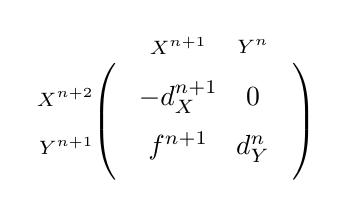
\begin{tikzpicture}[baseline]
			\matrix (M) [matrix of math nodes, ampersand replacement=\&, left delimiter=(, right delimiter=)] {
					-d_X^{n+1} \& 0 \\
					f^{n+1} \& d_Y^n \\
				};
				\node[above=1.2em] at (M-1-1) {\scriptsize $X^{n+1}$};
				\node[above=1.2em] at (M-1-2) {\scriptsize $Y^n$};
				\node[left=2.7em] at (M-1-1) {\scriptsize $X^{n+2}$};
				\node[left=2.7em] at (M-2-1) {\scriptsize $Y^{n+1}$};
		\end{tikzpicture} \\
		& : X^{n+1} \oplus Y^n \to X^{n+2} \oplus Y^{n+1} ,
	\end{align*}
	untuk $n\in\Z$. Karena $d_{X[1]}^n=-d_X^{n+1}$, tersedia pula notasi
	yang lebih ringkas
% segment-id: o014.li2.chapter3.mapping-cone.q002
	\[ \Cone(f) := \left( X[1] \oplus Y , \; \begin{pmatrix} d_{X[1]} & 0 \\ f[1] & d_Y \end{pmatrix} \right) . \]
\end{definisi}

% segment-id: o014.li2.chapter3.mapping-cone.p002
Mudah dibuktikan bahwa $\Cone(f)$ tetap merupakan kompleks, sebagaimana
ditunjukkan oleh perhitungan matriks berikut:
% segment-id: o014.li2.chapter3.mapping-cone.q003
\[ \begin{pmatrix} -d_X^{n+1} & 0 \\ f^{n+1} & d_Y^n \end{pmatrix} \begin{pmatrix} -d_X^n & 0 \\ f^n & d_Y^{n-1} \end{pmatrix} =
\begin{pmatrix} d_X^{n+1} d_X^n & 0 \\ - f^{n+1} d_X^n + d_Y^n f^n & d_Y^n d_Y^{n-1} \end{pmatrix}. \]

% segment-id: o014.li2.chapter3.mapping-cone.e001
\begin{contoh}
	Misalkan $f:X\to Y$ suatu morfisme dalam $\mathcal{A}$. Pandang $X,Y$
	sebagai objek $\cate{C}(\mathcal{A})$ (terkonsentrasi pada derajat $0$).
	Maka $\Cone(f)$ tepat merupakan kompleks $[X\xrightarrow{f}Y]$ (pada
	derajat $-1,0$, sedangkan semua suku lainnya sama dengan $0$).
\end{contoh}

% segment-id: o014.li2.chapter3.mapping-cone.p003
Kedua sifat funktorialitas berikut langsung diperoleh dari definisi.

% segment-id: o014.li2.chapter3.mapping-cone.pr001
\begin{proposisi}\label{prop:cone-functorial}
	Diberikan diagram komutatif dalam $\cate{C}(\mathcal{A})$
% segment-id: o014.li2.chapter3.mapping-cone.g001
	\[\begin{tikzcd}
		X \arrow[d, "f"'] \arrow[r, "\varphi"] & X' \arrow[d, "{f'}"] \\
		Y \arrow[r, "\psi"'] & Y'
	\end{tikzcd}\]
	maka $\bigl(\begin{smallmatrix} \varphi[1] & 0 \\ 0 & \psi \end{smallmatrix}\bigr)$
	memberikan morfisme $\Cone(f)\to\Cone(f')$.
\end{proposisi}

% segment-id: o014.li2.chapter3.mapping-cone.pr002
\begin{proposisi}\label{prop:Cone-A}
	Misalkan $F:\mathcal{A}\to\mathcal{A}'$ suatu funktor aditif dan
	$f:X\to Y$ suatu morfisme dalam $\cate{C}(\mathcal{A})$. Funktor yang
	bersesuaian $\cate{C}F:\cate{C}(\mathcal{A})\to
	\cate{C}(\mathcal{A}')$ memenuhi isomorfisme kanonik berikut dalam
	$\cate{C}(\mathcal{A}')$:
% segment-id: o014.li2.chapter3.mapping-cone.q004
	\[ (\cate{C}F)(\Cone(f)) \simeq \Cone(\cate{C}F(f)). \]
\end{proposisi}

% segment-id: o014.li2.chapter3.mapping-cone.p004
Kerucut pemetaan dapat ditempatkan dalam ``segitiga'' berikut, yang menjadi
landasan bagi seluruh teori selanjutnya.

% segment-id: o014.li2.chapter3.mapping-cone.d002
\begin{definisi}\label{def:cone-triangle}
	\index[sym1]{alphafbetaf@$\alpha(f), \beta(f)$}
	Tinjau suatu morfisme $f:X\to Y$ dalam $\cate{C}(\mathcal{A})$. Dari
	morfisme ini diperoleh morfisme-morfisme kanonik berikut dalam
	$\cate{C}(\mathcal{A})$:
% segment-id: o014.li2.chapter3.mapping-cone.q005
	\[ Y \xrightarrow{\alpha(f)} \Cone(f) \xrightarrow{\beta(f)} X[1] , \]
	yang secara eksplisit dinyatakan dengan matriks sebagai berikut:
% segment-id: o014.li2.chapter3.mapping-cone.q006
	\begin{align*}
		\alpha(f)^n & := \text{inklusi}\; \begin{pmatrix} 0 \\ \identity_{Y^n} \end{pmatrix}: Y^n \to X[1]^n \oplus Y^n , \\
		\beta(f)^n & := \text{proyeksi}\; \begin{pmatrix} \identity_{X[1]^n} & 0 \end{pmatrix}: X[1]^n \oplus Y^n \to X[1]^n .
	\end{align*}
	Jelas bahwa keduanya memang memberikan morfisme dalam
	$\cate{C}(\mathcal{A})$.
\end{definisi}

% segment-id: o014.li2.chapter3.mapping-cone.p005
Berikut ini dihimpun beberapa sifat homotopi kerucut pemetaan. Pertama-tama,
kita tunjukkan bahwa kerucut pemetaan dapat dipandang sebagai ``kokernel
homotopi'' atau ``kernel homotopi'' suatu morfisme. Inilah perwujudan pada
tingkat kompleks dari gagasan dasar dalam teori homotopi.

% segment-id: o014.li2.chapter3.mapping-cone.pr003
\begin{proposisi}\label{prop:homotopy-kernel-cokernel}
	Misalkan $f:X\to Y$ suatu morfisme dalam $\cate{C}(\mathcal{A})$. Terdapat
	bijeksi-bijeksi kanonik
% segment-id: o014.li2.chapter3.mapping-cone.g002
	\[\begin{tikzcd}[row sep=small]
		\Hom\left( \Cone(f), T \right) \arrow[leftrightarrow, r, "1:1"] & \left\{ (u, h): u \in \Hom(Y,T), \; h: \text{homotopi dari $uf$ ke $0$} \right\}, \\
		\Hom\left( T, \Cone(f)[-1] \right) \arrow[leftrightarrow, r, "1:1"] & \left\{ (v, k): v \in \Hom(T,X), \; k: \text{homotopi dari $fv$ ke $0$} \right\},
	\end{tikzcd}\]
	dengan $T$ sembarang objek $\cate{C}(\mathcal{A})$ dan
	$\Hom:=\Hom_{\cate{C}(\mathcal{A})}$. Secara lebih eksplisit,
% segment-id: o014.li2.chapter3.mapping-cone.l001
	\begin{compactitem}
% segment-id: o014.li2.chapter3.mapping-cone.i001
		\item citra $(u,h)$ dari $\tilde{u}:\Cone(f)\to T$ memenuhi
		$u=\tilde{u}\circ\alpha(f)$;
% segment-id: o014.li2.chapter3.mapping-cone.i002
		\item citra $(v,k)$ dari $\tilde{v}:T\to\Cone(f)[-1]$ memenuhi
		$v=\beta(f)[-1]\circ\tilde{v}$.
	\end{compactitem}
\end{proposisi}
% segment-id: o014.li2.chapter3.mapping-cone.pf001
\begin{bukti}
	Pertama-tama, tinjau kasus $\Hom\left(\Cone(f),T\right)$. Suatu morfisme
	$\tilde{u}:\Cone(f)\to T$ ekuivalen dengan keluarga morfisme dalam
	$\mathcal{A}$ berupa $h^n:X^{n+1}\to T^n$ dan $u^n:Y^n\to T^n$, dengan
	$n\in\Z$, yang memenuhi persamaan matriks
% segment-id: o014.li2.chapter3.mapping-cone.q007
	\[\begin{pmatrix}
		h^{n+1} & u^{n+1}
	\end{pmatrix} \begin{pmatrix}
		-d_X^{n+1} & 0 \\
		f^{n+1} & d_Y^n
	\end{pmatrix} = d_T^n \begin{pmatrix}
		h^n & u^n
	\end{pmatrix}. \]
	Setelah dijabarkan, persamaan ini ekuivalen dengan pernyataan bahwa
	$u=(u^n)_n:Y\to T$ merupakan morfisme dalam $\cate{C}(\mathcal{A})$ dan
	$h:=(h^{n-1})_n$ memenuhi
	$d_{\Hom^\bullet(X,T)}^{-1}h=uf$. Inilah bijeksi yang dimaksud; berdasarkan
	definisi $\alpha(f)$, persamaan $u=\tilde{u}\circ\alpha(f)$ langsung
	terlihat.

	Selanjutnya, tinjau suatu morfisme
	$\tilde{v}:T\to\Cone(f)[-1]$. Morfisme ini ekuivalen dengan keluarga
	morfisme dalam $\mathcal{A}$ berupa $v^n:T^n\to X^n$ dan
	$\underline{k}^n:T^n\to Y^{n-1}$ yang memenuhi
% segment-id: o014.li2.chapter3.mapping-cone.q008
	\[\begin{pmatrix}
		d_X^n & 0 \\
		-f^n & -d_Y^{n-1}
	\end{pmatrix} \begin{pmatrix}
		v^n \\ \underline{k}^n
	\end{pmatrix} = \begin{pmatrix}
		v^{n+1} \\ \underline{k}^{n+1}
	\end{pmatrix} d_T^n
	\quad (n \in \Z). \]
	Persamaan ini ekuivalen dengan pernyataan bahwa
	$v=(v^n)_n:T\to X$ merupakan morfisme dalam $\cate{C}(\mathcal{A})$ dan
	$k:=(-\underline{k}^n)_n$ memenuhi
	$d_{\Hom^\bullet(T,Y)}^{-1}k=fv$. Berdasarkan definisi $\beta(f)$,
	persamaan $v=\beta(f)[-1]\circ\tilde{v}$ juga langsung terlihat.
\end{bukti}

% segment-id: o014.li2.chapter3.mapping-cone.r001
\begin{catatan}[Kokernel homotopi dan kernel homotopi]\label{rem:homotopy-kernel-cokernel}
	\index{kokernel homotopi, kernel homotopi (homotopy cokernel, homotopy kernel)}
	Dari Proposisi~\ref{prop:homotopy-kernel-cokernel} diperoleh bahwa suatu
	morfisme $u:Y\to T$ (atau $v:T\to X$) memenuhi $uf$ (atau $fv$)
	homotopik nol jika dan hanya jika morfisme itu berfaktor melalui
	$\alpha(f):Y\to\Cone(f)$ (atau
	$\beta(f)[-1]:\Cone(f)[-1]\to X$). Hal ini dengan sendirinya mengingatkan
	kita pada sifat universal kokernel (atau kernel), dengan perbedaan berikut:
% segment-id: o014.li2.chapter3.mapping-cone.l002
	\begin{compactitem}
% segment-id: o014.li2.chapter3.mapping-cone.i003
		\item di sini syarat bahwa $uf$ (atau $fv$) homotopik nol menggantikan
		persamaan ketat $=0$;
% segment-id: o014.li2.chapter3.mapping-cone.i004
		\item faktorisasi $\tilde{u}$ (atau $\tilde{v}$) yang diberikan oleh
		proposisi tidak hanya membuktikan bahwa $uf$ (atau $fv$) homotopik nol,
		tetapi juga memuat cara morfisme itu dihomotopikan ke $0$; ini merupakan
		data satu tingkat lebih tinggi.
	\end{compactitem}
	Sifat-sifat ini tidak dapat ditangani begitu saja di
	$\cate{C}(\mathcal{A})$ atau $\cate{K}(\mathcal{A})$ dengan konsep-konsep
	dasar teori kategori; bahkan, kernel atau kokernel jarang ada dalam
	$\cate{K}(\mathcal{A})$. Oleh sebab itu, $Y\to\Cone(f)$ juga disebut
	\emph{kokernel homotopi} dari $f$, sedangkan
	$\beta(f)[-1]:\Cone(f)[-1]\to X$ disebut \emph{kernel homotopi} dari $f$.
	Menariknya, kerucut pemetaan $\Cone(f)$ beserta pergeserannya sekaligus
	memainkan peran ``kokernel'' dan ``kernel'' dalam pengertian ini.
\end{catatan}

% segment-id: o014.li2.chapter3.mapping-cone.p006
Suatu morfisme $f$ dalam $\cate{C}(\mathcal{A})$ disebut homotopik secara
kanonik dengan $g$ jika terdapat $h$ kanonik sedemikian sehingga
$g-f=d^{-1}h$; jika $f$ homotopik secara kanonik dengan $0$, maka morfisme
itu disebut homotopik nol secara kanonik.

% segment-id: o014.li2.chapter3.mapping-cone.pr004
\begin{proposisi}\label{prop:cone-homotopy}
	Misalkan $\mathcal{A}$ suatu kategori aditif.
% segment-id: o014.li2.chapter3.mapping-cone.l003
	\begin{enumerate}[(i)]
% segment-id: o014.li2.chapter3.mapping-cone.i005
		\item Jika $f:X\to Y$ suatu isomorfisme dalam
		$\cate{C}(\mathcal{A})$, maka $\identity_{\Cone(f)}$ homotopik nol
		secara kanonik.
% segment-id: o014.li2.chapter3.mapping-cone.i006
		\item Untuk sembarang morfisme $f:X\to Y$ dalam
		$\cate{C}(\mathcal{A})$, morfisme-morfisme dalam
		Definisi~\ref{def:cone-triangle} memenuhi
% segment-id: o014.li2.chapter3.mapping-cone.q009
		\[ \beta(f) \circ \alpha(f) = 0, \]
		sedangkan $\alpha(f)\circ f$ dan $f[1]\circ\beta(f)$ keduanya
		homotopik nol secara kanonik.
	\end{enumerate}
\end{proposisi}
% segment-id: o014.li2.chapter3.mapping-cone.pf002
\begin{bukti}
	Pertama-tama, tinjau (i). Berdasarkan funktorialitas kerucut pemetaan
	(Proposisi~\ref{prop:cone-functorial}), cukup meninjau
	$f=\identity_X$. Definisikan
% segment-id: o014.li2.chapter3.mapping-cone.q010
	\[ s^n := \begin{pmatrix} 0 & \identity_{X^n} \\ 0 & 0 \end{pmatrix} : X^{n+1} \oplus X^n \to X^n \oplus X^{n-1}, \quad n \in \Z. \]
	Perhitungan langsung memberikan
% segment-id: o014.li2.chapter3.mapping-cone.q011
	\begin{multline*}
		d^{n-1}_{\Cone(\identity_X)} s^n + s^{n+1} d^n_{\Cone(\identity_X)} = \\
		\begin{pmatrix} -d_X^n & 0 \\ \identity_{X^n} & d_X^{n-1} \end{pmatrix} \begin{pmatrix} 0 & \identity_{X^n} \\ 0 & 0 \end{pmatrix}  + \begin{pmatrix} 0 & \identity_{X^{n+1}} \\ 0 & 0 \end{pmatrix} \begin{pmatrix} -d_X^{n+1} & 0 \\ \identity_{X^{n+1}} & d_X^n \end{pmatrix}
		= \identity_{X^{n+1} \oplus X^n},
	\end{multline*}
	sehingga $s=(s^n)_{n\in\Z}$ menjadikan
	$\identity_{\Cone(\identity_X)}$ homotopik nol.

	Selanjutnya, tinjau (ii). Jelas bahwa
	$\beta(f)\circ\alpha(f)=0$. Homotopi-homotopi yang tersisa diperoleh dari
	Proposisi~\ref{prop:homotopy-kernel-cokernel}: ambil $T=\Cone(f)$, maka
	$\tilde{u}:=\identity_{\Cone(f)}\in\Hom(\Cone(f),T)$ menjadikan
	$\alpha(f)\circ f$ homotopik nol; ambil $T=\Cone(f)[-1]$, maka
	$\tilde{v}:=\identity_{\Cone(f)[-1]}\in\Hom(T,\Cone(f)[-1])$ menjadikan
	$f\circ\beta(f)[-1]$ homotopik nol, dan dengan demikian juga menjadikan
	$f[1]\circ\beta(f)$ homotopik nol.
\end{bukti}

% segment-id: o014.li2.chapter3.mapping-cone.p007
Definisi~\ref{def:cone-triangle} menghasilkan dua morfisme baru
$\alpha(f)$ dan $\beta(f)$ dari $f$. Hingga homotopi, kerucut pemetaan kedua
morfisme itu tidak menghasilkan objek baru; kita mulai dengan
$\Cone(\alpha(f))$ untuk menjelaskan hal tersebut. Pertama-tama, perhatikan
bahwa
% segment-id: o014.li2.chapter3.mapping-cone.q012
\[ \Cone(\alpha(f))^n = Y^{n+1} \oplus \Cone(f)^n = Y^{n+1} \oplus X^{n+1} \oplus Y^n. \]
Dalam notasi matriks,
% segment-id: o014.li2.chapter3.mapping-cone.q013
\begin{align*}
	\alpha(\alpha(f)) & = \begin{pmatrix}
		0 & 0 \\
		\identity_{X[1]} & 0 \\
		0 & \identity_Y
	\end{pmatrix} : \Cone(f) \to \Cone(\alpha(f)) , \\
	\beta(\alpha(f)) & = \begin{pmatrix}
		\identity_{Y[1]} & 0 & 0
	\end{pmatrix} : \Cone(\alpha(f)) \to Y[1].
\end{align*}

% segment-id: o014.li2.chapter3.mapping-cone.le001
\begin{lema}\label{prop:cone-alpha}
	Untuk suatu morfisme $f:X\to Y$ dalam $\cate{C}(\mathcal{A})$, notasi
	matriks mendefinisikan sepasang morfisme
% segment-id: o014.li2.chapter3.mapping-cone.g003
	\[ \begin{pmatrix} -f[1] \\ \identity_{X[1]} \\ 0 \end{pmatrix} : \begin{tikzcd} X[1] \arrow[r, shift left, "\phi"] & \Cone(\alpha(f)) \arrow[l, shift left, "\psi"] \end{tikzcd} : \begin{pmatrix} 0 & \identity_{X[1]} & 0 \end{pmatrix}. \]
	Keduanya memenuhi $\psi\circ\phi=\identity_{X[1]}$ dan menjadikan diagram
	berikut komutatif dalam $\cate{K}(\mathcal{A})$:
% segment-id: o014.li2.chapter3.mapping-cone.g004
	\[\begin{tikzcd}
		\Cone(f) \arrow[d, "{\identity_{\Cone(f)}}"'] \arrow[r, "\beta(f)"] & X[1] \arrow[d, "\phi"] \arrow[r, "{-f[1]}"] & Y[1] \arrow[d, "{\identity_{Y[1]}}"] \\
		\Cone(f) \arrow[r, "{\alpha(\alpha(f))}"'] & \Cone(\alpha(f)) \arrow[r, "\beta(\alpha(f))"'] & Y[1]
	\end{tikzcd}\]
	Selain itu, $\phi,\psi$ saling invers dalam $\cate{K}(\mathcal{A})$.
\end{lema}
% segment-id: o014.li2.chapter3.mapping-cone.pf003
\begin{bukti}
	Berdasarkan uraian sebelumnya tentang $\Cone(\alpha(f))$, dalam notasi
	matriks $d_{\Cone(\alpha(f))}^n$ diberikan oleh
% segment-id: o014.li2.chapter3.mapping-cone.q014
	\[ \begin{pmatrix} -d_Y^{n+1} & 0 & 0 \\ 0 & -d_X^{n+1} & 0 \\ \identity_{Y^{n+1}} & f^{n+1} & d_Y^n \end{pmatrix} : Y^{n+1} \oplus X^{n+1} \oplus Y^n \to Y^{n+2} \oplus X^{n+2} \oplus Y^{n+1}. \]
	Cukup diverifikasi pernyataan-pernyataan berikut dalam
	$\cate{C}(\mathcal{A})$:
% segment-id: o014.li2.chapter3.mapping-cone.l004
	\begin{itemize}
% segment-id: o014.li2.chapter3.mapping-cone.i007
		\item $\phi:=(\phi^n)_{n\in\Z}$ dan $\psi:=(\psi^n)_{n\in\Z}$
		keduanya merupakan morfisme kompleks;
% segment-id: o014.li2.chapter3.mapping-cone.i008
		\item $\psi\circ\phi=\identity_{X[1]}$;
% segment-id: o014.li2.chapter3.mapping-cone.i009
		\item $\psi\circ\alpha(\alpha(f))=\beta(f)$;
% segment-id: o014.li2.chapter3.mapping-cone.i010
		\item $\beta(\alpha(f))\circ\phi=-f[1]$;
% segment-id: o014.li2.chapter3.mapping-cone.i011
		\item terdapat
		$s=(s^n)_{n\in\Z}\in\Hom^{-1}\left(\Cone(\alpha(f)),
		\Cone(\alpha(f))\right)$ sedemikian sehingga
		$\identity_{\Cone(\alpha(f))}-\phi\circ\psi
		=d^{-1}_{\Hom^\bullet}(s)$.
	\end{itemize}
	Empat pernyataan pertama bersifat elementer. Untuk pernyataan terakhir,
	ambillah, dalam notasi matriks,
% segment-id: o014.li2.chapter3.mapping-cone.q015
	\[ s^n := \begin{pmatrix} 0 & 0 & \identity_{Y^n} \\ 0 & 0 & 0 \\ 0 & 0 & 0 \end{pmatrix}: \Cone(\alpha(f))^n \to \Cone(\alpha(f))^{n-1} \]
	dan lakukan verifikasi langsung.
\end{bukti}

% segment-id: o014.li2.chapter3.mapping-cone.p008
Untuk kasus $\beta(f)$, kita melakukan sedikit modifikasi dan meninjau
kerucut pemetaan dari $-\beta(f)[-1]:\Cone(f)[-1]\to X$.

% segment-id: o014.li2.chapter3.mapping-cone.d003
\begin{definisi}\label{def:Cyl}
	\index{silinder pemetaan (mapping cylinder)}
	\index[sym1]{Cylf@$\Cyl(f)$}
	Untuk suatu morfisme $f:X\to Y$ dalam $\cate{C}(\mathcal{A})$,
	\emph{silinder pemetaan} dari $f$ didefinisikan sebagai
% segment-id: o014.li2.chapter3.mapping-cone.q016
	\[ \Cyl(f) := \Cone\left( \Cone(f)[-1] \xrightarrow{-\beta(f)[-1]} X \right). \]
	Silinder ini dilengkapi morfisme-morfisme kanonik
	$X\to\Cyl(f)\to\Cone(f)$.
\end{definisi}

% segment-id: o014.li2.chapter3.mapping-cone.p009
Silinder pemetaan mempunyai funktorialitas yang bentuknya sama dengan
funktorialitas kerucut pemetaan (Proposisi~\ref{prop:cone-functorial}).
Berdasarkan Catatan~\ref{rem:homotopy-kernel-cokernel}, $\Cyl(f)$ dapat
dibandingkan dengan kocitra dalam kategori aditif---objek ini kurang lebih
merupakan ``kokernel dari kernel'' (Proposisi~\ref{prop:Im-Coim-additive})---
sehingga dapat pula dipandang sebagai kocitra homotopi dari $f$.

% segment-id: o014.li2.chapter3.mapping-cone.p010
Secara lebih eksplisit,
$\Cyl(f)^n=\Cone(f)^n\oplus X^n=X^{n+1}\oplus Y^n\oplus X^n$; morfisme
$X\to\mathrm{Cyl}(f)$ (atau $\mathrm{Cyl}(f)\to\Cone(f)$) ialah inklusi ke
suku ketiga pada jumlah langsung (atau proyeksi ke dua suku pertama), dan
% segment-id: o014.li2.chapter3.mapping-cone.q017
\[ d_{\Cyl(f)}^n =
	\begin{pmatrix} d_{\Cone(f)}^n & 0 \\ -\beta(f)^n & d_X^n \end{pmatrix}
	= \begin{pmatrix}
		-d_X^{n+1} & 0 & 0 \\
		f^{n+1} & d_Y^n & 0 \\
		-\identity_{X^{n+1}} & 0 & d_X^n
\end{pmatrix} .\]

% segment-id: o014.li2.chapter3.mapping-cone.le002
\begin{lema}\label{prop:cone-beta}
	Untuk suatu morfisme $f:X\to Y$ dalam $\cate{C}(\mathcal{A})$, dapat
	didefinisikan sepasang morfisme
% segment-id: o014.li2.chapter3.mapping-cone.g005
	\[ \begin{pmatrix} 0 \\ \identity_Y \\ 0 \end{pmatrix} : \begin{tikzcd} Y \arrow[r, shift left, "\phi"] & \Cyl(f) \arrow[l, shift left, "\psi"] \end{tikzcd} : \begin{pmatrix} 0 & \identity_Y & f \end{pmatrix}. \]
	Keduanya memenuhi $\psi\circ\phi=\identity_Y$ dan menjadikan diagram
	berikut komutatif dalam $\cate{K}(\mathcal{A})$:
% segment-id: o014.li2.chapter3.mapping-cone.g006
	\[\begin{tikzcd}
		X \arrow[d, "{\identity_X}"'] \arrow[r, "f"] & Y \arrow[d, "\phi"] \arrow[r, "{\alpha(f)}"] & \Cone(f) \arrow[d, "{\identity_{\Cone(f)}}"] \\
		X \arrow[r] & \Cyl(f) \arrow[r] & \Cone(f)
	\end{tikzcd}\]
	Selain itu, $\phi,\psi$ saling invers dalam $\cate{K}(\mathcal{A})$.
Lebih lanjut, $f$ berfaktor sebagai komposisi
$X\to\Cyl(f)\xrightarrow{\psi}Y$.
\end{lema}
% segment-id: o014.li2.chapter3.mapping-cone.pf004
\begin{bukti}
	Pembaca dapat memverifikasi langsung dari definisi bahwa $\phi$ dan $\psi$
	memang memberikan morfisme kompleks. Setelah itu,
	$\psi\circ\phi=\identity_Y$ langsung terlihat. Selanjutnya, untuk
	membuktikan bahwa $\phi$ dan $\psi$ saling invers dalam
	$\cate{K}(\mathcal{A})$, seperti pada Lema~\ref{prop:cone-alpha}, ambillah
% segment-id: o014.li2.chapter3.mapping-cone.q018
	\begin{align*}
		s^n & := \begin{pmatrix} 0 & 0 & -\identity_{X^n} \\ 0 & 0 & 0 \\ 0 & 0 & 0 \end{pmatrix}: X^{n+1} \oplus Y^n \oplus X^n \to X^n \oplus Y^{n-1} \oplus X^{n-1}, \\
		s & := (s^n)_{n \in \Z},
	\end{align*}
	dan verifikasi
	$\identity_{\Cyl(f)}-\phi\circ\psi=d^{-1}_{\Hom^\bullet}(s)$.

	Kotak kanan pada diagram sudah komutatif dalam $\cate{C}(\mathcal{A})$.
	Untuk kotak kiri, cukup perhatikan bahwa komposisi
	$X\to\mathrm{Cyl}(f)\xrightarrow{\psi}Y$ sama dengan $f$.
\end{bukti}

% segment-id: o014.li2.chapter3.mapping-cone.p011
Lema~\ref{prop:cone-alpha} bersama Lema~\ref{prop:cone-beta} menunjukkan
bahwa, hingga isomorfisme dalam $\cate{K}(\mathcal{A})$, sembarang morfisme
$f:X\to Y$ dapat diganti dengan proyeksi yang jauh lebih sederhana
$\Cone(\alpha(f))[-1]\to Y$ (atau inklusi $X\to\Cyl(f)$), dan konstruksi ini
funktorial dalam $f$. Inilah suatu gagasan penting dalam aljabar homologis
dan teori homotopi.

% segment-id: o014.li2.chapter3.mapping-cone.p012
Kasus khusus silinder pemetaan dengan $f=\identity_X$ mempunyai kegunaan lain:
silinder itu dapat digunakan untuk menafsirkan homotopi. Bagi pembaca yang
mengenal teori homologi, semua ini mempunyai tafsiran topologis, tetapi di
sini kita hanya membahas versi aljabarnya.

% segment-id: o014.li2.chapter3.mapping-cone.pr005
\begin{proposisi}\label{prop:cylinder-homotopy}
	\index[sym1]{CylX@$\Cyl_X$}
	Misalkan $X$ suatu objek $\cate{C}(\mathcal{A})$ dan definisikan
	$\mathrm{Cyl}_X:=\mathrm{Cyl}(\identity_X)$. Perhatikan bahwa
	$\mathrm{Cyl}_X^n=X^{n+1}\oplus X^n\oplus X^n$.
% segment-id: o014.li2.chapter3.mapping-cone.l005
	\begin{enumerate}[(i)]
% segment-id: o014.li2.chapter3.mapping-cone.i012
		\item Dalam $\cate{C}(\mathcal{A})$ terdapat morfisme-morfisme
% segment-id: o014.li2.chapter3.mapping-cone.g007
		$\begin{tikzcd}
			X \arrow[shift left, r, "i_0"] \arrow[shift right, r, "i_1"'] & \Cyl_X \arrow[r, "j"] & X
		\end{tikzcd}$,
		yang dalam notasi matriks didefinisikan untuk setiap $n\in\Z$ oleh
% segment-id: o014.li2.chapter3.mapping-cone.q019
		\begin{equation*}
			i_0^n := \begin{pmatrix} 0 \\ 0 \\ \identity_{X^n} \end{pmatrix} , \quad
			i_1^n := \begin{pmatrix} 0 \\ \identity_{X^n} \\ 0 \end{pmatrix} , \quad j^n := \begin{pmatrix} 0 & \identity_{X^n} & \identity_{X^n} \end{pmatrix},
		\end{equation*}
		Morfisme-morfisme ini memenuhi $ji_0=\identity_X=ji_1$, dan citra $j$
		dalam $\cate{K}(\mathcal{A})$ merupakan isomorfisme.
% segment-id: o014.li2.chapter3.mapping-cone.i013
		\item Untuk sembarang objek $Y$ dari $\cate{C}(\mathcal{A})$, terdapat
		bijeksi
% segment-id: o014.li2.chapter3.mapping-cone.q020
		\begin{align*}
			\left\{\begin{array}{r|l}
				(f, g, h) & f, g \in \Hom_{\cate{C}(\mathcal{A})}(X, Y) \\
				& h \in \Hom^{-1}(X, Y) \\
				& g - f = d^{-1}_{\Hom^\bullet(X, Y)} h
			\end{array}\right\} & \xrightarrow{1:1} \Hom_{\cate{C}(\mathcal{A})}\left( \mathrm{Cyl}_X, Y \right) \\
			(f, g, h) & \longmapsto \tilde{h} = (\tilde{h}^n)_{n \in \Z}, \; \tilde{h}^n := \begin{pmatrix} h^n & g^n & f^n \end{pmatrix}.
		\end{align*}
		Secara khusus, $f=\tilde{h}i_0$ dan $g=\tilde{h}i_1$.
	\end{enumerate}
\end{proposisi}
% segment-id: o014.li2.chapter3.mapping-cone.pf005
\begin{bukti}
	Untuk (i), perhatikan bahwa $i_0$ tidak lain ialah morfisme kanonik
	$X\to\mathrm{Cyl}(\identity_X)$ dalam Definisi~\ref{def:Cyl}, sedangkan
	$i_1$ ialah morfisme $\phi:X\to\mathrm{Cyl}(\identity_X)$ dalam
	Lema~\ref{prop:cone-beta}. Diagram komutatif dalam
	Lema~\ref{prop:cone-beta} menunjukkan bahwa keduanya memberikan
	isomorfisme yang sama dalam $\cate{K}(\mathcal{A})$.

	Untuk $j$, mudah diverifikasi bahwa
	$j^{n+1}d_{\Cyl_X}^n=\bigl(0\;d_X^n\;d_X^n\bigr)=d_X^nj^n$.
	Jadi, $j$ memang merupakan morfisme, sedangkan
	$ji_0=\identity_X=ji_1$ langsung terlihat. Karena $i_0$ dan $i_1$
	merupakan isomorfisme dalam $\cate{K}(\mathcal{A})$, demikian pula $j$.

	Untuk (ii), tuliskan sembarang unsur $\tilde{h}$ dari
	$\Hom^0(\mathrm{Cyl}_X,Y)$ dalam bentuk
	\[
		\tilde{h}=\left((h^n,g^n,f^n)\right)_{n\in\Z},
	\]
	dengan
% segment-id: o014.li2.chapter3.mapping-cone.q021
	\[ h^n: X^{n+1} \to Y^n, \quad f^n: X^n \to Y^n, \quad g^n: X^n \to Y^n \]
	semuanya merupakan morfisme dalam $\mathcal{A}$. Dengan menghilangkan
	superskrip dan menggunakan notasi matriks, hitung
% segment-id: o014.li2.chapter3.mapping-cone.q022
	\begin{align*}
		\tilde{h} \; d_{\mathrm{Cyl}_X} & = \begin{pmatrix} h & g & f \end{pmatrix} \begin{pmatrix} -d_X & 0 & 0 \\ \identity_X & d_X & 0 \\ -\identity_X & 0 & d_X \end{pmatrix} = \begin{pmatrix} -hd_X + g - f & g d_X & f d_X \end{pmatrix} , \\
		d_Y \; \tilde{h} & = \begin{pmatrix} d_Y h & d_Y g & d_Y f \end{pmatrix}.
	\end{align*}
	Oleh karena itu, $\tilde{h}$ merupakan morfisme kompleks jika dan hanya
	jika $f,g\in\Hom_{\cate{C}(\mathcal{A})}(X,Y)$ dan
	$g-f=hd_X+d_Yh$.
\end{bukti}

% segment-id: o014.li2.chapter3.mapping-cone.r002
\begin{catatan}\label{rem:cone-chain}
	\index{kerucut pemetaan}\index{silinder pemetaan}
	Kerucut pemetaan dan silinder pemetaan tentu saja mempunyai versi untuk
	kompleks rantai (lihat Catatan~\ref{rem:cochain-vs-chain}). Diberikan suatu
	morfisme kompleks rantai $f:X\to Y$, definisikan
% segment-id: o014.li2.chapter3.mapping-cone.q023
	\[\begin{array}{rlrl}
		\Cone(f)_n & :=(X[-1] \oplus Y)_n, &
		\Cyl(f)_n & := (X[-1] \oplus Y \oplus X)_n, \\
		d_{\Cone(f)} & := \begin{pmatrix} d_{X[-1]} & 0 \\ f[-1] & d_Y \end{pmatrix}, &
		d_{\Cyl(f)} & := \begin{pmatrix} d_{X[-1]} & 0 & 0 \\ f[-1] & d_Y & 0 \\ -\identity_{X[-1]} & 0 & d_X \end{pmatrix}.
	\end{array}\]

	Semua pernyataan dalam bagian ini dapat dipindahkan ke kasus kompleks
	rantai. Secara khusus, terdapat morfisme-morfisme kanonik
% segment-id: o014.li2.chapter3.mapping-cone.q024
	\[ X \xrightarrow{f} Y \xrightarrow{\alpha(f)} \Cone(f) \xrightarrow{\beta(f)} X[-1], \quad X \to \Cyl(f) \to \Cone(f). \]
\end{catatan}

% Unit 035 terjemahan Bahasa Indonesia dari chapter3.tex baris 622--699.
% Sumber: Methods of Algebra, Volume 2, commit
% 9a5803ff77dd3257484cb177f851a73770a59dd3 (CC BY 4.0).
% stable-unit-id: o014.aljabr2.chapter3.opposite-category-complexes
% Cakupan: Bagian 3.4 lengkap.

% segment-id: o014.li2.chapter3.opposite-category-complexes.h001
\section{Kompleks pada kategori lawan}\label{sec:opposite-cplx}
\hypertarget{o014.aljabr2.chapter3.opposite-category-complexes}{ }

% segment-id: o014.li2.chapter3.opposite-category-complexes.p001
Tetapkan suatu kategori aditif $\mathcal{A}$. Bagian ini bertujuan
menghubungkan kompleks pada $\mathcal{A}$ dan $\mathcal{A}^{\opp}$. Karena
funktor yang melibatkan $\mathcal{A}^{\opp}$, misalnya funktor $\Hom$, sering
muncul, prosedur ini sederhana tetapi perlu; beberapa tanda positif dan
negatif yang terlibat juga memerlukan sedikit perhatian. Pembaca pemula
disarankan melewati bagian ini atau sekadar membacanya sepintas terlebih
dahulu.

% segment-id: o014.li2.chapter3.opposite-category-complexes.p002
Pembahasan berikut terbagi menjadi tiga aspek: kompleks, homotopi, dan kerucut
pemetaan. Versi untuk kategori turunan yang akan dikaji kemudian
(Proposisi~\sourcecrossref{prop:derived-cat-op}{pada pembahasan kategori turunan selanjutnya})
merupakan penerapan langsung hasil-hasil
ini. Ingat bahwa jika $f:X\to Y$ suatu morfisme dalam $\mathcal{A}$, maka
$f^{\opp}$ menyatakan morfisme yang bersesuaian $Y\to X$ dalam
$\mathcal{A}^{\opp}$.

% segment-id: o014.li2.chapter3.opposite-category-complexes.dp001
\begin{definisiproposisi}\label{def:sigma}
	\index[sym1]{sigma@$\sigma$}
	Isomorfisme antarkategori aditif
	$\sigma:\cate{C}(\mathcal{A}^{\opp})\to\cate{C}(\mathcal{A})^{\opp}$
	didefinisikan sebagai berikut. Untuk suatu objek $X$ dalam
	$\cate{C}(\mathcal{A}^{\opp})$, definisikan di dalam $\mathcal{A}$
% segment-id: o014.li2.chapter3.opposite-category-complexes.q001
	\[ (\sigma X)^n := X^{-n}, \quad d_{\sigma X}^n = (-1)^{n+1} \left[ d_X^{-n-1, \opp}: (\sigma X)^n \to (\sigma X)^{n+1} \right], \quad n \in \Z. \]
	Untuk suatu morfisme
	$f=\left(f^n:X^n\to Y^n\right)_n$ dalam
	$\cate{C}(\mathcal{A}^{\opp})$, citranya $\sigma f$ diambil sebagai
	morfisme berikut dalam $\cate{C}(\mathcal{A})$:
% segment-id: o014.li2.chapter3.opposite-category-complexes.q002
	\[ (\sigma f)^n := \left(f^{-n} \right)^{\opp} : (\sigma Y)^n \to (\sigma X)^n, \]
	yakni sebagai morfisme $\sigma X\to\sigma Y$ dalam
	$\cate{C}(\mathcal{A})^{\opp}$. Untuk setiap $m\in\Z$, terdapat
	isomorfisme alami
% segment-id: o014.li2.chapter3.opposite-category-complexes.q003
	\[ s_m: \sigma \circ [m] \rightiso [-m] \circ \sigma, \]
	dengan $[-m]$ dipandang sebagai funktor dari
	$\cate{C}(\mathcal{A})^{\opp}$ ke dirinya sendiri (secara ketat, notasinya
	seharusnya $[-m]^{\opp}$).
\end{definisiproposisi}
% segment-id: o014.li2.chapter3.opposite-category-complexes.pf001
\begin{bukti}
	Kasus umum $s_m$ dapat direduksi secara bertahap ke kasus $m=1$.
	Definisikan $s_1=(s_{1,X})_X$ sebagai berikut. Untuk setiap $n$, ambil
% segment-id: o014.li2.chapter3.opposite-category-complexes.g001
	\begin{equation}\label{eqn:sigma-s}\begin{tikzcd}[row sep=tiny]
		s_{1,X}^n : \sigma(X{[1]})^n = X^{1-n} \arrow[r, "\sim"', "{(-1)^{n-1}}" inner sep=0.6em] & X^{1-n} = (\sigma X){[-1]}^n .
	\end{tikzcd}\end{equation}
	Seluruh verifikasi tereduksi pada
	$s_{1, X}^{n+1} d^n_{\sigma(X[1])} = -d_{X[1]}^{-n-1, \opp} =
	d_X^{-n, \opp} = (-1)^n d_{\sigma X}^{n-1} =
	d^n_{(\sigma X)[-1]} s_{1,X}^n$.
\end{bukti}

% segment-id: o014.li2.chapter3.opposite-category-complexes.p003
Jika konstruksi $\sigma$ dengan koefisien $(-1)^{n+1}$ diterapkan pada kedua
arah, $\sigma^2X$ isomorfik secara alami dengan $X$ melalui isomorfisme yang
komponen berderajat $n$-nya adalah $(-1)^n\identity_{X^n}$. Untuk memperoleh
invers, definisikan konstruksi arah balik dengan rumus yang sama pada objek
dan morfisme, tetapi gunakan koefisien $(-1)^n$ pada diferensial. Komposisi
dalam kedua urutan tepat sama dengan funktor identitas, sehingga $\sigma$
memang merupakan isomorfisme antarkategori.%
\footnote{Catatan penerjemah (O014-C036): sumber, dengan alasan
$n(n+1)\equiv0\pmod{2}$, menyatakan bahwa penerapan $\sigma$ dua kali
langsung mengembalikan $X$. Namun, penggunaan rumus yang sama pada kedua arah
memberikan diferensial $-d_X$, bukan $d_X$. Target mencatat isomorfisme alami
bertanda dan konstruksi invers yang dikoreksi di atas.}

% segment-id: o014.li2.chapter3.opposite-category-complexes.r001
\begin{catatan}\label{rem:sigma-vs-cohomology}
	Jika $\mathcal{A}$ kategori abelian, tanda pada $d_{\sigma X}^\bullet$
	tidak mengubah kohomologi yang diperkenalkan dalam
	Definisi~\ref{def:cohomology}; dengan demikian,
	$\Hm^{-n}(\sigma X)\in\Obj(\mathcal{A})$ bersesuaian dengan
	$\Hm^n(X)\in\Obj(\mathcal{A}^{\opp})$.
\end{catatan}

% segment-id: o014.li2.chapter3.opposite-category-complexes.p004
Selanjutnya, kita kaji hubungan antara $\sigma$ dan homotopi.

% segment-id: o014.li2.chapter3.opposite-category-complexes.pr001
\begin{proposisi}\label{prop:sigma-homotopy}
	Funktor $\sigma$ yang didefinisikan di atas menginduksi ekuivalensi
	antarkategori aditif
	$\cate{K}(\mathcal{A}^{\opp})\rightiso\cate{K}(\mathcal{A})^{\opp}$.
\end{proposisi}
% segment-id: o014.li2.chapter3.opposite-category-complexes.pf002
\begin{bukti}
	Tetapkan objek $X,Y$ dalam $\cate{C}(\mathcal{A}^{\opp})$. Untuk
	$f=(f^k)_k\in\Hom^{-1}_{\cate{C}(\mathcal{A}^{\opp})}(X,Y)$, gunakan
	tabel berikut untuk mendefinisikan $\sigma f$ yang bersesuaian dalam
	$\mathcal{A}$, dengan
	$\sigma f\in\Hom^{-1}_{\cate{C}(\mathcal{A})}(\sigma Y,\sigma X)$:
% segment-id: o014.li2.chapter3.opposite-category-complexes.q004
	\begingroup\setlength{\arraycolsep}{4pt}
	\[\begin{array}{|c|c|c|c|} \hline
		\text{Kategori} & \multicolumn{3}{c|}{\text{Morfisme}} \\ \hline
		\mathcal{A}^{\opp} & X^k \xrightarrow{(-1)^{k+1} f^k} Y^{k-1} & d_Y^{k-1} f^k + f^{k+1} d_X^k & (d^{-1}f)^k \\
		\mathcal{A} & (\sigma Y)^{-k+1} \xrightarrow{(\sigma f)^{-k+1}} (\sigma X)^{-k} & (\sigma f)^{-k+1} d_{\sigma Y}^{-k} + d_{\sigma X}^{-k-1} (\sigma f)^{-k} & d^{-1} (\sigma f)^{-k} \\ \hline
	\end{array}\]
	\endgroup
	Hal ini cukup untuk menunjukkan
	\[\begin{aligned}
		\Hom_{\cate{K}(\mathcal{A}^{\opp})}(X, Y)
		&\rightiso \Hom_{\cate{K}(\mathcal{A})}(\sigma Y, \sigma X) \\
		&= \Hom_{\cate{K}(\mathcal{A})^{\opp}}(\sigma X, \sigma Y).
	\end{aligned}\]
\end{bukti}

% segment-id: o014.li2.chapter3.opposite-category-complexes.p005
Terakhir, melalui $\sigma$ dan keluarga isomorfisme $(s_m)_m$ yang dibangun
di atas, kita bandingkan kerucut pemetaan dalam $\cate{C}(\mathcal{A})$ dan
$\cate{C}(\mathcal{A}^{\opp})$. Rinciannya berupa perhitungan yang agak rutin.

% segment-id: o014.li2.chapter3.opposite-category-complexes.pr002
\begin{proposisi}\label{prop:sigma-triangulated}
	\index[sym1]{sigma}
	Untuk setiap morfisme $f:X\to Y$ dalam
	$\cate{C}(\mathcal{A}^{\opp})$, terdapat diagram komutatif berikut dalam
	$\cate{C}(\mathcal{A})$% 
	\footnote{Di sini $\alpha(\cdot)$ dan $\beta(\cdot)$ keduanya didefinisikan
	relatif terhadap $\cate{C}(\mathcal{A})$. Jika diagram dipandang dalam
	$\cate{C}(\mathcal{A})^{\opp}$, semua panahnya harus dibalik.}:
% segment-id: o014.li2.chapter3.opposite-category-complexes.g002
	\[\begin{tikzcd}[column sep=large]
		\sigma\left( X{[1]} \right) \arrow[r, "{\sigma(\beta(f))}"] \arrow[d, "{s_{1,X}}"'] & \sigma\left(\Cone(f)\right) \arrow[r, "{\sigma(\alpha(f))}"] \arrow[d, "\theta"] & \sigma Y \arrow[r, "\sigma(f)"] \arrow[d, "\identity"] & \sigma X \arrow[d, "{\identity}"] \\
		(\sigma X){[-1]} \arrow[r, "{\alpha(\sigma(f))[-1]}"' inner sep=0.6em] & \Cone(\sigma(f)){[-1]} \arrow[r, "{\beta(\sigma(f))[-1]}"' inner sep=0.6em] & \sigma Y \arrow[r, "{\sigma(f)}"' inner sep=0.6em] & \sigma X
	\end{tikzcd}\]
	dengan $\theta$ suatu isomorfisme kanonik dan $s_{1,X}$ isomorfisme yang
	diberikan oleh Definisi--Proposisi~\ref{def:sigma}.
\end{proposisi}
% segment-id: o014.li2.chapter3.opposite-category-complexes.pf003
\begin{bukti}
	Jika $\Cone(f)$ diganti dengan $X[1]\oplus Y$, pernyataannya mudah dan
	isomorfisme yang diperlukan cukup diambil sebagai
	$(s_{1,X},\identity_{\sigma Y})$. Kesulitannya di sini ialah bahwa matriks
	$d_{\Cone(f)}$ mempunyai entri luar diagonal $f[1]$. Meskipun demikian,
	kita tetap mengikuti cara yang sama: dengan menggunakan
	\eqref{eqn:sigma-s}, untuk setiap $n\in\Z$ definisikan isomorfisme
% segment-id: o014.li2.chapter3.opposite-category-complexes.q005
	\begin{multline*}
		\theta^n: \sigma\left(\Cone(f)\right)^n = \sigma\left(X[1]\right)^n \oplus (\sigma Y)^n \\
		\xrightarrow[\sim]{(s_{1,X}, \identity)^n = ((-1)^{n-1} \identity, \identity) } (\sigma X)[-1]^n \oplus (\sigma Y)^n \xlongequal{\text{pertukaran}} \left( (\sigma Y) \oplus (\sigma X)[-1] \right)^n ,
	\end{multline*}	
	Dengan identifikasi ini, morfisme $d_{\sigma(\Cone(f))}^n$ dalam
	$\mathcal{A}$ bersesuaian dengan
% segment-id: o014.li2.chapter3.opposite-category-complexes.q006
	\[ \begin{pmatrix}
		d_{\sigma Y}^n & 0 \\
		* & d_{(\sigma X)[-1]}^n
	\end{pmatrix} : \left( (\sigma Y) \oplus (\sigma X)[-1] \right)^n \to \left( (\sigma Y) \oplus (\sigma X)[-1] \right)^{n+1} . \]
	Seperti dinyatakan pada awal bukti, entri-entri diagonal tidak bermasalah;
	yang perlu ditentukan ialah entri kiri bawah matriks tersebut. Berdasarkan
	Definisi--Proposisi~\ref{def:sigma}, entri ini sama dengan $(-1)^{n+1}$
	dikali komposisi morfisme berikut dalam $\mathcal{A}$:
% segment-id: o014.li2.chapter3.opposite-category-complexes.g003
	\[\begin{tikzcd}[row sep=tiny]
		(\sigma Y)^n \arrow[r] & (\sigma(X[1]))^{n+1} \arrow[r, "\sim"] & (\sigma X)[-1]^{n+1} \\
		Y^{-n} \arrow[equal, u] \arrow[r, "{(f^{-n})^{\opp}}"'] & X^{-n} \arrow[equal, u] \arrow[r, "{s_{1, X}^{n+1} = (-1)^n}"'] & X^{-n} \arrow[equal, u]
	\end{tikzcd}\]
	Dengan demikian, hasilnya ialah $-\sigma(f)^n$. Oleh karena itu,
% segment-id: o014.li2.chapter3.opposite-category-complexes.q007
	\[ \theta := (\theta^n)_{n \in \Z}: \sigma(\Cone(f)) \rightiso \Cone(\sigma(f))[-1] \]
	memang merupakan isomorfisme dalam $\cate{C}(\mathcal{A})$. Setelah hal
	ini ditetapkan, verifikasi komutativitas tidak lagi mengandung kesulitan
	yang berarti.
\end{bukti}

% segment-id: o014.li2.chapter3.opposite-category-complexes.p006
Tentu saja, hasil-hasil bagian ini juga berlaku untuk kompleks rantai dan
dapat diperumum ke kasus ketika $\mathcal{A}$ merupakan kategori
$\Bbbk$-linear.

% Unit 036 terjemahan Bahasa Indonesia dari chapter3.tex baris 700--945.
% Sumber: Methods of Algebra, Volume 2, commit
% 9a5803ff77dd3257484cb177f851a73770a59dd3 (CC BY 4.0).
% stable-unit-id: o014.aljabr2.chapter3.double-complexes
% Cakupan: Bagian 3.5 lengkap.

% segment-id: o014.li2.chapter3.double-complexes.h001
\section{Bikompleks}\label{sec:double-cplx}
\hypertarget{o014.aljabr2.chapter3.double-complexes}{ }

% segment-id: o014.li2.chapter3.double-complexes.p001
Dalam bagian ini, $\mathcal{A}$ tetap merupakan kategori aditif. Secara kasar,
bikompleks dapat dibayangkan sebagai versi dua dimensi dari kompleks, dengan
diferensial dalam arah vertikal dan horizontal.

% segment-id: o014.li2.chapter3.double-complexes.d001
\begin{definisi}[Bikompleks]\label{def:double-cplx}
	\index{bikompleks (double complex)}
	\index[sym1]{dhoridvert@$\dhori$, $\dvert$}
	Bikompleks pada kategori aditif $\mathcal{A}$ terdiri atas keluarga objek
	$\left(X^{p,q}\right)_{(p,q)\in\Z^2}$ dalam $\mathcal{A}$, bersama dengan
	morfisme $\dhori^{p,q}:X^{p,q}\to X^{p+1,q}$ dan
	$\dvert^{p,q}:X^{p,q}\to X^{p,q+1}$, yang memenuhi
% segment-id: o014.li2.chapter3.double-complexes.q001
	\[ \dhori^{p+1,q} \dhori^{p,q} = 0, \quad \dvert^{p, q+1} \dvert^{p,q} = 0, \quad \dhori^{p, q+1} \dvert^{p,q} = \dvert^{p+1, q} \dhori^{p,q}. \]
	Data di atas biasanya disingkat sebagai
	$(X^{\bullet,\bullet},\dhori,\dvert)$, $X^{\bullet,\bullet}$, atau $X$.
\end{definisi}

% segment-id: o014.li2.chapter3.double-complexes.p002
Syarat-syarat pada $\dhori,\dvert$ dapat disingkat menjadi
% segment-id: o014.li2.chapter3.double-complexes.q002
\[ \dhori^2 = 0, \quad \dvert^2 = 0, \quad \dhori \dvert = \dvert \dhori. \]

% segment-id: o014.li2.chapter3.double-complexes.d002
\begin{definisi}\label{def:bicplx}
	Diberikan kategori aditif $\mathcal{A}$, suatu morfisme dari bikompleks $X$
	ke $Y$ adalah keluarga morfisme
% segment-id: o014.li2.chapter3.double-complexes.q003
	\[ f = \left( f^{p,q}: X^{p, q} \to Y^{p, q} \right)_{(p, q) \in \Z^2}, \]
	sedemikian sehingga, untuk semua $p,q$, berlaku
% segment-id: o014.li2.chapter3.double-complexes.q004
	\[ \dhori_Y^{p, q} f^{p, q} = f^{p+1, q} \dhori_X^{p, q}, \quad \dvert_Y^{p, q} f^{p, q} = f^{p, q+1} \dvert_X^{p, q}. \]
	Relasi-relasi di atas dapat disingkat sebagai
	$\dhori_Yf=f\dhori_X$ dan $\dvert_Yf=f\dvert_X$.
\end{definisi}

% segment-id: o014.li2.chapter3.double-complexes.p003
Seperti dalam Proposisi~\ref{prop:additive-cat-cplx}, definisi-definisi ini
menjadikan semua bikompleks pada $\mathcal{A}$ suatu kategori aditif
$\cate{C}^2(\mathcal{A})$.
\index[sym1]{C2A@$\cate{C}^2(\mathcal{A})$}

% segment-id: o014.li2.chapter3.double-complexes.p004
Secara visual, bikompleks $X$ digambarkan sebagai
% segment-id: o014.li2.chapter3.double-complexes.g001
\[\begin{tikzcd}
	& \vdots & \vdots & \\
	\cdots \arrow[r] & X^{p, q+1} \arrow[r] \arrow[u] & X^{p+1, q+1} \arrow[r] \arrow[u] & \cdots \\
	\cdots \arrow[r] & X^{p, q} \arrow[r, "{\dhori^{p,q}}"'] \arrow[u, "{\dvert^{p,q}}"] & X^{p+1, q} \arrow[r] \arrow[u] & \cdots \\
	& \vdots \arrow[u] & \vdots \arrow[u] &
\end{tikzcd}\]
Setiap baris $\left(X^{\bullet,q},d^{\bullet,q}\right)$ dan setiap kolom
$\left(X^{p,\bullet},d^{p,\bullet}\right)$ merupakan kompleks. Dengan
demikian, bikompleks dapat dipandang menurut kolom ataupun menurut baris.

% segment-id: o014.li2.chapter3.double-complexes.d003
\begin{definisi}\label{def:bicplx-F1}
	\index[sym1]{F1F2@$F_{\mathrm{I}}, F_{\mathrm{II}}$}
	Funktor aditif
	$F_{\mathrm{I}}:\cate{C}^2(\mathcal{A})\to
	\cate{C}(\cate{C}(\mathcal{A}))$ didefinisikan sebagai berikut: untuk
	bikompleks $X$, ambil $(F_{\mathrm{I}}X)^p=X^{p,\bullet}$ dan
	$d_{F_{\mathrm{I}}X}^p=\dhori^{p,\bullet}:(F_{\mathrm{I}}X)^p\to
	(F_{\mathrm{I}}X)^{p+1}$. Demikian pula, rumus
	$(F_{\mathrm{II}}X)^q=X^{\bullet,q}$ dan
	$d_{F_{\mathrm{II}}X}^q=\dvert^{\bullet,q}$ mendefinisikan funktor aditif
	$\cate{C}^2(\mathcal{A})\to\cate{C}(\cate{C}(\mathcal{A}))$. Di sini
	$p,q\in\Z$.
\end{definisi}

% segment-id: o014.li2.chapter3.double-complexes.p005
Definisi~\ref{def:bicplx} menyiratkan bahwa $F_{\mathrm{I}}$ dan
$F_{\mathrm{II}}$ keduanya merupakan isomorfisme antarkategori aditif. Hal
ini digambarkan sebagai berikut:
% segment-id: o014.li2.chapter3.double-complexes.g002
\begin{equation}\label{eqn:bicplx-diagram}\begin{tikzcd}[
		/tikz/execute at end picture={
			\node[rectangle, draw, fit=(NW) (SE), inner xsep=0.5em, inner ysep=0em] {};
		}]
		\vdots & |[alias=NW]| & {} & \\
		(F_{\mathrm{II}} X)^q \arrow[u, "{d^q_{F_{\mathrm{II}} X}}"] \arrow[phantom, r, ":=" description, sloped] & \cdots \arrow[r] & X^{p,q} \arrow[r, "{\dhori^{p,q}}"'] \arrow[u, "{\dvert^{p,q}}"] & \cdots \\
		\vdots \arrow[u] & & {} \arrow[u] & |[alias=SE]| \\
		& \cdots \arrow[r] & (F_{\mathrm{I}} X)^p \arrow[r, "{d^p_{F_{\mathrm{I}} X}}"] \arrow[phantom, u, ":=" description, sloped] & \cdots
\end{tikzcd}\end{equation}

% segment-id: o014.li2.chapter3.double-complexes.d004
\begin{definisi}[Kompleks total]\label{def:total-cplx}
	\index{kompleks total (total complex)}
	\index[sym1]{tot@$\tot_{\oplus}$, $\tot_{\Pi}$, $\tot$}
	Misalkan $\mathcal{A}$ mempunyai koproduk terhitung, yang dinotasikan
	dengan simbol jumlah langsung $\bigoplus$, dan misalkan $X$ objek
	$\cate{C}^2(\mathcal{A})$. Definisikan kompleks $\tot_{\oplus}(X)$ pada
	$\mathcal{A}$ sebagai berikut:
% segment-id: o014.li2.chapter3.double-complexes.l001
	\begin{compactitem}
% segment-id: o014.li2.chapter3.double-complexes.i001
		\item $\tot_{\oplus}(X)^n := \bigoplus_{p+q=n} X^{p, q}$,
% segment-id: o014.li2.chapter3.double-complexes.i002
		\item restriksi $d^n:\tot_{\oplus}(X)^n\to
		\tot_{\oplus}(X)^{n+1}$ pada suku $X^{p,q}$ sama dengan
		$\dhori^{p,q}+(-1)^p\dvert^{p,q}$.
	\end{compactitem}
\end{definisi}

% segment-id: o014.li2.chapter3.double-complexes.p006
Dengan menghilangkan superskrip, penulisan lengkap
$d^2:X^{p,q}\to X^{p+2,q}\oplus X^{p+1,q+1}\oplus X^{p,q+2}$ memberikan
% segment-id: o014.li2.chapter3.double-complexes.q005
\[ d^2 = \left( \dhori^2, \; (-1)^p \dhori \dvert + (-1)^{p+1} \dvert \dhori , \; \dvert^2 \right) = (0, 0, 0). \]

% segment-id: o014.li2.chapter3.double-complexes.p007
Jika koproduk dalam konstruksi funktor $\tot_{\oplus}$ diganti dengan produk
$\prod$, secara serupa diperoleh
$\tot_{\Pi}X\in\Obj(\cate{C}(\mathcal{A}))$, asalkan produk-produk yang
diperlukan ada. Definisi
$d^n:\tot_{\Pi}(X)^n\to\tot_{\Pi}(X)^{n+1}$ serupa dengan kasus
$\tot_{\oplus}$: kita mensyaratkan bahwa proyeksi $d^{n-1}$ ke $X^{p,q}$
sama dengan komposisi
% segment-id: o014.li2.chapter3.double-complexes.q006
\[ \tot_{\Pi}^{n-1}(X) \xrightarrow{\text{proyeksi}} X^{p-1, q} \oplus X^{p,q-1} \xrightarrow{(\dhori^{p-1, q}, (-1)^p \dvert^{p, q-1})} X^{p, q} \]
tersebut; dengan cara yang sama diperoleh $d^2=0$. Jika tidak menimbulkan
kerancuan, $\tot_{\oplus}X$ dan $\tot_{\Pi}X$ keduanya disebut
\emph{kompleks total} dari $X$.

% segment-id: o014.li2.chapter3.double-complexes.p008
Sifat berikut seharusnya sudah jelas.

% segment-id: o014.li2.chapter3.double-complexes.pr001
\begin{proposisi}
	Dengan syarat-syarat yang bersesuaian, $\tot_{\oplus}$ dan $\tot_{\Pi}$
	keduanya merupakan funktor aditif dari $\cate{C}^2(\mathcal{A})$ ke
	$\cate{C}(\mathcal{A})$.
\end{proposisi}

% segment-id: o014.li2.chapter3.double-complexes.p009
Dalam definisi kompleks total, superskrip $p$ dan $q$ sepintas tampak tidak
simetris. Untuk menghilangkan kesan ini, kita definisikan automorfisme aditif
$\mathrm{swap}$ pada $\cate{C}^2(\mathcal{A})$ sedemikian sehingga
$\mathrm{swap}(X)^{p,q}=X^{q,p}$ serta $\dhori$ dan $\dvert$ saling
dipertukarkan. Tanda $(-1)^{pq}$ yang akan menyertainya pada hakikatnya
merupakan mekanisme yang sama dengan aturan tanda Koszul dalam
\cite[Definisi--Teorema~7.4.4]{Li1}.

\index[sym1]{swap@$\mathrm{swap}$}
% segment-id: o014.li2.chapter3.double-complexes.pr002
\begin{proposisi}\label{prop:double-cplx-swap}
	Untuk setiap $(p,q)\in\Z^2$ dan objek $X$ dalam
	$\cate{C}^2(\mathcal{A})$, definisikan keluarga isomorfisme
% segment-id: o014.li2.chapter3.double-complexes.q007
	\[ r^{p, q}_X := (-1)^{pq} \identity_{X^{p,q}} : X^{p, q} \to \mathrm{swap}(X)^{q,p} . \]
% segment-id: o014.li2.chapter3.double-complexes.l002
	\begin{compactitem}
% segment-id: o014.li2.chapter3.double-complexes.i003
		\item Jika $\mathcal{A}$ mempunyai koproduk terhitung, maka
		$(r_X^{p,q})_{(p,q)\in\Z^2}$ menginduksi isomorfisme
		$r_X:\tot_{\oplus}(X)\rightiso\tot_{\oplus}(\mathrm{swap}(X))$.
% segment-id: o014.li2.chapter3.double-complexes.i004
		\item Jika $\mathcal{A}$ mempunyai produk terhitung, maka
		$(r_X^{p,q})_{(p,q)\in\Z^2}$ menginduksi isomorfisme
		$r_X:\tot_{\Pi}(X)\rightiso\tot_{\Pi}(\mathrm{swap}(X))$.
	\end{compactitem}
\end{proposisi}
% segment-id: o014.li2.chapter3.double-complexes.pf001
\begin{bukti}
	Untuk semua $(p,q)\in\Z^2$, diagram
% segment-id: o014.li2.chapter3.double-complexes.g003
	\[\begin{tikzcd}[row sep=large]
		X^{p,q} \arrow[d, "(-1)^{pq} \identity"'] \arrow[r, "{ (\dhori, (-1)^p \dvert) }" inner sep=0.8em] & X^{p+1, q} \oplus X^{p, q+1} \arrow[d, "{((-1)^{(p+1)q} \identity, (-1)^{p(q+1)} \identity) }"] \\
		X^{p,q} \arrow[r, "{((-1)^q \dhori, \dvert)}"' inner sep=0.8em] & X^{p+1, q} \oplus X^{p, q+1}
	\end{tikzcd}\]
	komutatif, sehingga $r_X$ memang merupakan morfisme kompleks.
\end{bukti}

% segment-id: o014.li2.chapter3.double-complexes.p010
Syarat adanya koproduk terhitung (atau produk terhitung) dalam definisi
$\tot_{\oplus}X$ (atau $\tot_{\Pi}X$) dapat diperlemah: jika untuk setiap
$n$ hanya ada paling banyak sejumlah hingga pasangan $(p,q)$ yang memenuhi
$p+q=n$ dan $X^{p,q}\neq0$, maka koproduk (atau produk) dalam definisi
kompleks total menjadi jumlah langsung hingga. Dalam hal ini, kedua kompleks
total dapat dinotasikan seragam sebagai $\tot(X)$. Pembahasan lebih lanjut
akan diberikan setelah Definisi~\sourcecrossref{def:Cf-Supp}{pada \S~3.10}.

% segment-id: o014.li2.chapter3.double-complexes.r001
\begin{catatan}\label{rem:k-fold-cplx}
	Dengan gagasan yang sama, untuk setiap $k\in\Z_{\geq1}$ dapat didefinisikan
	kompleks lipat-$k$ sebagai data
% segment-id: o014.li2.chapter3.double-complexes.q008
	\[ \left( X^{p_1, \ldots, p_k} \in \Obj(\mathcal{A}) \right)_{p_1, \ldots, p_k \in \Z}, \quad {}^1 d, \ldots, {}^k d, \]
	dengan ${}^i d^{p_1,\ldots,p_k}:X^{p_1,\ldots,p_k}\to
	X^{p_1,\ldots,p_i+1,\ldots,p_k}$ dan
% segment-id: o014.li2.chapter3.double-complexes.q009
	\[ {}^i d^2 = 0, \quad {}^i d {}^j d = {}^j d {}^i d \quad \text{(superskrip dihilangkan)}. \]
	Semua kompleks lipat-$k$ membentuk kategori aditif
	$\cate{C}^k(\mathcal{A})$. Dengan mengikuti
	Definisi~\ref{def:bicplx-F1}, dapat pula didefinisikan keluarga funktor
	aditif $F_i:\cate{C}^k(\mathcal{A})\to
	\cate{C}(\cate{C}^{k-1}(\mathcal{A}))$ sedemikian sehingga setiap $F_i$
	merupakan ekuivalensi antarkategori ($k\geq2$ dan $i=1,\ldots,k$).
	
	Dalam keadaan ini, jika $\mathcal{A}$ mempunyai koproduk atau produk
	terhitung, funktor kompleks total dapat didefinisikan dengan cara serupa:
% segment-id: o014.li2.chapter3.double-complexes.q010
	\[ \tot_{\oplus} \; \text{atau} \; \tot_{\Pi}: \cate{C}^k(\mathcal{A}) \to \cate{C}(\mathcal{A}). \]
	Rinciannya sama dengan kasus bikompleks dan tidak perlu diuraikan lagi.
\end{catatan}

% segment-id: o014.li2.chapter3.double-complexes.p011
Definisikan isomorfisme dari $\cate{C}^2(\mathcal{A})$ ke dirinya sendiri
$[m]_{\mathrm{I}}:=F_{\mathrm{I}}^{-1}\circ[m]\circ F_{\mathrm{I}}$ dan
$[m]_{\mathrm{II}}:=F_{\mathrm{II}}^{-1}\circ[m]\circ F_{\mathrm{II}}$,
yang masing-masing bersesuaian dengan pergeseran horizontal dan vertikal
bikompleks. Untuk semua $a,b\in\Z$ berlaku
$[a]_{\mathrm{I}}[b]_{\mathrm{II}}=[b]_{\mathrm{II}}[a]_{\mathrm{I}}$.
Sekarang kita kaji pengaruh funktor-funktor ini terhadap kompleks total serta
hubungannya dengan automorfisme $\mathrm{swap}$.

% segment-id: o014.li2.chapter3.double-complexes.n001
% Reference: KS06, p.290
% segment-id: o014.li2.chapter3.double-complexes.pr003
\begin{proposisi}\label{prop:tot-shift}
	Untuk semua $X\in\Obj(\cate{C}^2(\mathcal{A}))$ dan
	$(p,q)\in\Z^2$, notasikan pembenaman standar
	$X^{p,q}\hookrightarrow\mathrm{tot}_{\oplus}(X)^{p+q}$ dengan
	$\iota_{p,q}$. Untuk setiap $n\in\Z$, definisikan
% segment-id: o014.li2.chapter3.double-complexes.l003
	\begin{itemize}
% segment-id: o014.li2.chapter3.double-complexes.i005
		\item $\theta_X^n:\tot_{\oplus}\left(X[1]_{\mathrm{I}}\right)^n\to
		\tot_{\oplus}(X)[1]^n$ sedemikian sehingga restriksinya pada
		$X[1]_{\mathrm{I}}^{p,q}=X^{p+1,q}$ sama dengan $\iota_{p+1,q}$;
% segment-id: o014.li2.chapter3.double-complexes.i006
		\item $(\theta'_X)^n:\tot_{\oplus}\left(X[1]_{\mathrm{II}}\right)^n
		\to\tot_{\oplus}(X)[1]^n$ sedemikian sehingga restriksinya pada
		$X[1]_{\mathrm{II}}^{p,q}=X^{p,q+1}$ sama dengan
		$(-1)^p\iota_{p,q+1}$.
	\end{itemize}
	Keduanya memberikan isomorfisme kanonik dalam $\cate{C}(\mathcal{A})$:
% segment-id: o014.li2.chapter3.double-complexes.q011
	\begin{align*}
		\theta_X & = (\theta_X^n)_n: \tot_{\oplus} \left( X[1]_{\mathrm{I}} \right) \rightiso \tot_{\oplus} \left(X\right)[1], \\
		\theta'_X & = ((\theta'_X)^n)_n: \tot_{\oplus} \left( X[1]_{\mathrm{II}} \right) \rightiso \tot_{\oplus} \left(X\right)[1],
	\end{align*}
	beserta diagram antikomutatif (yakni, kedua komposisinya berselisih tanda
	negatif)
% segment-id: o014.li2.chapter3.double-complexes.g004
	\[\begin{tikzcd}
		\tot_{\oplus} \left( X[1]_{\mathrm{I}}[1]_{\mathrm{II}}\right) \arrow[r, "{\theta_{X[1]_{\mathrm{II}}}}" inner sep=0.6em] \arrow[d, "{\theta'_{X[1]_{\mathrm{I}}}}"'] & \tot_{\oplus}\left(X[1]_{\mathrm{II}}\right)[1] \arrow[d, "{\theta'_X [1]}"] \\
		\tot_{\oplus} \left( X[1]_{\mathrm{I}}\right)[1] \arrow[r, "{\theta_X [1]}"' inner sep=0.6em] & \tot_{\oplus}(X)[2]
	\end{tikzcd}\]
	dan diagram komutatif
% segment-id: o014.li2.chapter3.double-complexes.g005
	\[\begin{tikzcd}[column sep=large]
		\tot_{\oplus} \left( X[1]_{\mathrm{I}}[1]_{\mathrm{II}} \right) \arrow[r, "\text{$\theta$ lalu $\theta'$}"] \arrow[d, "{r_{X[1]_{\mathrm{I}}[1]_{\mathrm{II}}}}"'] & \tot_{\oplus}(X)[2] \arrow[d, "{r_X[2]}"] \\
		\tot_{\oplus}\left( \mathrm{swap}(X)[1]_{\mathrm{I}}[1]_{\mathrm{II}} \right) \arrow[r, "\text{$\theta'$ lalu $\theta$}"'] & \tot_{\oplus}\left(\mathrm{swap}(X)\right)[2],
	\end{tikzcd}\]
	dengan $r$ sebagaimana didefinisikan dalam
	Proposisi~\ref{prop:double-cplx-swap}. Jika $\tot_{\oplus}$ diganti dengan
	$\tot_{\Pi}$, tetap diperoleh $\theta_X,\theta'_X$ yang sama beserta diagram
	antikomutatif yang bersesuaian.
\end{proposisi}
% segment-id: o014.li2.chapter3.double-complexes.pf002
\begin{bukti}
	Verifikasi langsung berdasarkan definisi kompleks total
	(Definisi~\ref{def:total-cplx}) dan definisi funktor pergeseran
	(Definisi~\ref{def:translation-functor}) menunjukkan bahwa $\theta_X$ dan
	$\theta'_X$ merupakan morfisme kompleks; rinciannya panjang tetapi tidak
	sulit. Diagram antikomutatif tereduksi pada pengamatan bahwa diagram
% segment-id: o014.li2.chapter3.double-complexes.g006
	\[\begin{tikzcd}
		X^{p+1, q+1} \arrow[d, "{(-1)^p \identity}"'] \arrow[r, "\identity"] & X^{p+1, q+1} \arrow[d, "{(-1)^{p+1} \identity}"] \\
		X^{p+1, q+1} \arrow[r, "\identity"'] & X^{p+1, q+1}
	\end{tikzcd}\]
	antikomutatif.
	
	Sekarang tinjau pernyataan tentang diagram komutatif. Tetapkan
	$(p,q)\in\Z^2$ dan bandingkan restriksi kedua komposisi pada
	$(X[1]_{\mathrm{I}}[1]_{\mathrm{II}})^{p,q}$. Telah dijelaskan bahwa
	$\theta$ lalu $\theta'$ (untuk $X$) dan $\theta'$ lalu $\theta$ (untuk
	$\mathrm{swap}(X)$) masing-masing memberikan
% segment-id: o014.li2.chapter3.double-complexes.q012
	\[ (-1)^{p+1}, \; (-1)^q \; \in \Aut(X^{p+1, q+1}) \quad \text{($\identity$ dihilangkan)}. \]
	Di sisi lain, restriksi $r_{X[1]_{\mathrm{I}}[1]_{\mathrm{II}}}$ dan
	$r_X[2]$ pada $X^{p+1,q+1}$ masing-masing adalah $(-1)^{pq}$ dan
	$(-1)^{(p+1)(q+1)}$. Namun,
	$(p+1)(q+1)-pq\equiv(p+1)-q\pmod{2}$. Terbukti.
\end{bukti}

% segment-id: o014.li2.chapter3.double-complexes.p012
Sebagai perumuman sederhana dari diagram antikomutatif di atas, pembaca
diminta membuktikan bahwa, untuk semua $a,b\in\Z$, kedua morfisme
% segment-id: o014.li2.chapter3.double-complexes.q013
\[ \tot_{\oplus}(X[a]_{\mathrm{I}}[b]_{\mathrm{II}}) \rightrightarrows \tot_{\oplus}(X)[a+b] \]
yang didefinisikan dengan kedua urutan ($\theta$ lalu $\theta'$ dan $\theta'$
lalu $\theta$) berselisih tanda $(-1)^{ab}$; di sisi lain, diagram komutatif
di atas tetap berlaku untuk $X[a]_{\mathrm{I}}[b]_{\mathrm{II}}$. Pernyataan
yang sama berlaku jika $\tot_{\oplus}$ diganti dengan $\tot_{\Pi}$.

% segment-id: o014.li2.chapter3.double-complexes.p013
Salah satu penggunaan utama bikompleks ialah dalam kajian bifunktor. Apakah
yang dimaksud dengan bifunktor?

% segment-id: o014.li2.chapter3.double-complexes.c001
\begin{konvensi}\label{con:bifunctor}
	\index{bifunktor (bifunctor)}
	Funktor berbentuk $F:\mathcal{A}_1\times\mathcal{A}_2\to\mathcal{B}$
	disebut \emph{bifunktor}. Setelah objek
	$X_i\in\Obj(\mathcal{A}_i)$ ditetapkan, diperoleh funktor satu variabel
	$F(X_1,\cdot):\mathcal{A}_2\to\mathcal{B}$ dan
	$F(\cdot,X_2):\mathcal{A}_1\to\mathcal{B}$. Dengan demikian, dapat dibahas
	keaditifan, keeksakan, dan berbagai konsep lain bagi setiap variabel $F$.
\end{konvensi}

% segment-id: o014.li2.chapter3.double-complexes.dp001
\begin{definisiproposisi}\label{def:bifunctor-cplx}
	\index[sym1]{C2F@$\cate{C}^2 F, \cate{C}_{\oplus} F, \cate{C}_{\Pi} F$}
	Misalkan $\mathcal{A}_1,\mathcal{A}_2,\mathcal{B}$ kategori-kategori
	aditif dan $F:\mathcal{A}_1\times\mathcal{A}_2\to\mathcal{B}$ suatu
	bifunktor yang aditif dalam setiap variabel. Terdapat funktor yang
	bersesuaian
% segment-id: o014.li2.chapter3.double-complexes.g007
	\[\begin{tikzcd}[row sep=tiny, column sep=small]
		\cate{C}^2 F: \cate{C}(\mathcal{A}_1) \times \cate{C}(\mathcal{A}_2) \arrow[r] & \cate{C}^2(\mathcal{B}) \\
		(X, Y) \arrow[mapsto, r] & (F(X, Y))^{p, q} := F(X^p, Y^q), \\
		& \dhori^{p, q} = F\left( d_X^p, \identity \right), \; \dvert^{p, q} = F\left( \identity, d_Y^q\right) .
	\end{tikzcd}\]

	Oleh karena itu, jika $\mathcal{B}$ mempunyai koproduk terhitung atau
	produk terhitung, masing-masing dapat didefinisikan
% segment-id: o014.li2.chapter3.double-complexes.q014
	\begin{gather*}
		\cate{C}_{\oplus} F := \tot_{\oplus} \circ \cate{C}^2 F: \cate{C}(\mathcal{A}_1) \times \cate{C}(\mathcal{A}_2) \to \cate{C}(\mathcal{B}), \\
		\cate{C}_{\Pi} F := \tot_{\Pi} \circ \cate{C}^2 F: \cate{C}(\mathcal{A}_1) \times \cate{C}(\mathcal{A}_2) \to \cate{C}(\mathcal{B}).
	\end{gather*}
	Jika $\tot_{\oplus}$ dan $\tot_{\Pi}$ yang dibahas hanya melibatkan
	jumlah langsung hingga, maka $\cate{C}_{\oplus}F=\cate{C}_{\Pi}F$.%
	\footnote{Catatan penerjemah (O014-C038): sumber menghilangkan $F$ dari
	kesetaraan ini dan dari suku paling kanan pada dua isomorfisme di bawah.
	Karena funktor yang didefinisikan ialah $\cate{C}_{\oplus}F$ dan
	$\cate{C}_{\Pi}F$, target memulihkan $F$ pada ketiga tempat tersebut.}
\end{definisiproposisi}
% segment-id: o014.li2.chapter3.double-complexes.pf003
\begin{bukti}
	Syarat bikompleks $\dhori\dvert=\dvert\dhori$ langsung mengikuti definisi
	bifunktor; selebihnya jelas.
\end{bukti}

% segment-id: o014.li2.chapter3.double-complexes.p014
Kategori bikompleks juga mempunyai konsep homotopi. Misalkan
$f,g:X\to Y$ sepasang morfisme dalam $\cate{C}^2(\mathcal{A})$. Homotopi
dari $f$ ke $g$ adalah dua keluarga morfisme yang memenuhi syarat-syarat
berikut. \index{homotopi!versi bikompleks}
% segment-id: o014.li2.chapter3.double-complexes.q015
\begin{equation*}\begin{gathered}
% segment-id: o014.li2.chapter3.double-complexes.g008
\begin{tikzcd}
	Y^{p-1, q} & X^{p,q} \arrow[l, "{h^{p,q}}"'] \arrow[d, "{k^{p, q}}"] \\
	& Y^{p, q-1}
\end{tikzcd} \qquad (p,q) \in \Z^2 , \\
	\dvert^{p-1, q} h^{p, q} = h^{p, q+1} \dvert^{p, q}, \qquad \dhori^{p, q-1} k^{p,q} = k^{p+1, q} \dhori^{p,q}, \\
	g^{p,q} - f^{p, q} = \dhori^{p-1, q} h^{p,q} + h^{p+1, q} \dhori^{p,q} + \dvert^{p, q-1} k^{p,q} + k^{p, q+1} \dvert^{p,q}.
\end{gathered}\end{equation*}
Hal ini beralasan: dari $\dvert h=h\dvert$, $\dhori k=k\dhori$, dan definisi
bikompleks, mudah diperiksa bahwa
$\dhori h+h\dhori+\dvert k+k\dvert$ selalu memberikan morfisme dalam
$\cate{C}^2(\mathcal{A})$.

% segment-id: o014.li2.chapter3.double-complexes.p015
Homotopi bikompleks tercermin pada kompleks total. Lebih tepatnya, setelah
$(h^{p,q},k^{p,q})_{p,q\in\Z}$ diberikan, dapat didefinisikan
$\hat{h}\in\Hom^{-1}\left(\tot_{\oplus}(X),\tot_{\oplus}(Y)\right)$
sedemikian sehingga restriksi $\hat{h}$ pada suku jumlah langsung $X^{p,q}$
sama dengan
% segment-id: o014.li2.chapter3.double-complexes.q016
\[ \left( h^{p,q}, (-1)^p k^{p,q} \right): X^{p,q} \to Y^{p-1, q} \oplus Y^{p, q-1}, \]
yang menjadikan
$\tot_{\oplus}(g)-\tot_{\oplus}(f)=d^{-1}\hat{h}$; kasus $\tot_{\Pi}$
ditangani dengan cara yang sama.

% segment-id: o014.li2.chapter3.double-complexes.p016
Dengan demikian, relasi homotopi bikompleks mendefinisikan
$\cate{K}^2(\mathcal{A})$ beserta funktor
$\cate{C}^2(\mathcal{A})\to\cate{K}^2(\mathcal{A})$. Jika koproduk terhitung
(atau produk terhitung) ada, funktor $\tot_{\oplus}$ (atau $\tot_{\Pi}$)
turun menjadi funktor
$\cate{K}^2(\mathcal{A})\to\cate{K}(\mathcal{A})$.
\index[sym1]{K2A@$\cate{K}^2(\mathcal{A})$}

% segment-id: o014.li2.chapter3.double-complexes.p017
Kembali ke bifunktor $F:\mathcal{A}_1\times\mathcal{A}_2\to\mathcal{B}$
di antara kategori-kategori aditif, dan andaikan $F$ aditif dalam setiap
variabel. Berikut adalah versi bifunktor dari \eqref{eqn:KF}.

% segment-id: o014.li2.chapter3.double-complexes.pr004
\begin{proposisi}\label{prop:bifunctor-cplx-homotopy}
	\index[sym1]{K2F@$\cate{K}^2 F, \cate{K}_{\oplus} F, \cate{K}_{\Pi} F$}
	Ambil bifunktor $F$ seperti di atas. Maka $\cate{C}^2F$ berfaktor melalui
	$\cate{K}^2F:\cate{K}(\mathcal{A}_1)\times\cate{K}(\mathcal{A}_2)\to
	\cate{K}^2(\mathcal{B})$.
	
	Demikian pula, $\cate{C}_{\oplus}F$ atau $\cate{C}_{\Pi}F$ berfaktor
	melalui $\cate{K}(\mathcal{A}_1)\times\cate{K}(\mathcal{A}_2)\to
	\cate{K}(\mathcal{B})$, dan masing-masing dinotasikan dengan
	$\cate{K}_{\oplus}F$ atau $\cate{K}_{\Pi}F$, asalkan funktor
	$\cate{C}_{\oplus}F$ atau $\cate{C}_{\Pi}F$ terdefinisi.
\end{proposisi}
% segment-id: o014.li2.chapter3.double-complexes.pf004
\begin{bukti}
	Ambil kasus $\cate{C}_{\oplus}F$ sebagai contoh. Yang perlu ditunjukkan
	ialah bahwa, untuk morfisme homotopik nol
	$f_1=d^{-1}g:X_1\to Y_1$ dalam $\cate{C}(\mathcal{A}_1)$ dan sebarang
	morfisme $f_2:X_2\to Y_2$ dalam $\cate{C}(\mathcal{A}_2)$, morfisme yang
	bersesuaian $(\cate{C}^2F)(f_1,f_2):\cate{C}^2F(X_1,X_2)\to
	\cate{C}^2F(Y_1,Y_2)$ homotopik nol. Pilihan yang jelas ialah
	$h^{p,q}:=F(g^p,f_2^q)$ dan $k^{p,q}:=0$. Karena $f_2$ merupakan morfisme,
	$h$ memang berkomutasi dengan $\dvert=F(\identity,d)$. Variabel kedua
	ditangani dengan cara serupa.
\end{bukti}

% segment-id: o014.li2.chapter3.double-complexes.p018
Proposisi~\ref{prop:tot-shift} memberikan isomorfisme kanonik
% segment-id: o014.li2.chapter3.double-complexes.q017
\begin{gather*}
	\cate{C}_{\oplus} F(X[1], Y) \simeq \cate{C}_{\oplus}F(X, Y)[1] \simeq \cate{C}_{\oplus}F(X, Y[1]), \\
	\cate{K}_{\oplus} F(X[1], Y) \simeq \cate{K}_{\oplus}F(X, Y)[1] \simeq \cate{K}_{\oplus}F(X, Y[1]).
\end{gather*}
Pernyataan yang sama berlaku jika $\oplus$ diganti dengan $\Pi$.

% segment-id: o014.li2.chapter3.double-complexes.e001
\begin{contoh}[Bikompleks $\Hom$]\label{eg:Hom-bicplx}
	\index{bikompleks Hom@bikompleks $\Hom$ ($\Hom$ double complex)}
	\index[sym1]{Hombb@$\Hom^{\bullet, \bullet}$}
	Tinjau bifunktor
	$\Hom(\cdot,\cdot):\mathcal{A}^{\opp}\times\mathcal{A}\to\cate{Ab}$,
	yang memetakan pasangan objek $(S,T)$ ke $\Hom_{\mathcal{A}}(S,T)$.
	Berikut ini akan ditunjukkan bahwa kompleks $\Hom$, yaitu
	$\Hom^\bullet(X,Y)$, isomorfik secara kanonik dengan nilai pada objek
	$(X,Y)$ dari funktor komposit
% segment-id: o014.li2.chapter3.double-complexes.q018
	\[ \cate{C}(\mathcal{A})^{\opp} \times \cate{C}(\mathcal{A}) \xrightarrow{(\sigma^{-1}, \identity)} \cate{C}(\mathcal{A}^{\opp}) \times \cate{C}(\mathcal{A}) \xrightarrow{\cate{C}_{\Pi} \Hom(\cdot, \cdot)} \cate{C}(\cate{Ab}) \]
	dengan $\sigma$ sebagaimana dalam
	Definisi--Proposisi~\ref{def:sigma}.

	Untuk itu, pertama-tama tinjau bifunktor
	$F:\mathcal{A}\times\mathcal{A}^{\opp}\to\cate{Ab}$ yang didefinisikan
	dengan $F(T,S)=\Hom_{\mathcal{A}}(S,T)$, serta funktor komposit
% segment-id: o014.li2.chapter3.double-complexes.q019
	\[ \cate{C}(\mathcal{A}) \times \cate{C}(\mathcal{A})^{\opp} \xrightarrow{(\identity, \sigma^{-1})} \cate{C}(\mathcal{A}) \times \cate{C}(\mathcal{A}^{\opp}) \xrightarrow{\cate{C}^2 F} \cate{C}^2(\cate{Ab}). \]
	Misalkan $X,Y\in\Obj(\cate{C}(\mathcal{A}))$. Citra objek $(Y,X)$ oleh
	funktor komposit di atas disebut \emph{bikompleks $\Hom$} dan dinotasikan
	dengan $\Hom^{\bullet,\bullet}(X,Y)$. Berdasarkan diagram komutatif yang
	jelas
% segment-id: o014.li2.chapter3.double-complexes.g009
	\[\begin{tikzcd}[column sep=large]
		\cate{C}(\mathcal{A})^{\opp} \times \cate{C}(\mathcal{A}) \arrow[d, "\simeq"', "\text{pertukaran}"] \arrow[r, "{(\sigma^{-1}, \identity)}" inner sep=0.6em] & \cate{C}(\mathcal{A}^{\opp}) \times \cate{C}(\mathcal{A}) \arrow[r, "{\cate{C}^2 \Hom(\cdot, \cdot)}" inner sep=0.6em] \arrow[d, "\simeq"', "\text{pertukaran}"] & \cate{C}^2(\cate{Ab}) \arrow[d, "\mathrm{swap}"] \\
		\cate{C}(\mathcal{A}) \times \cate{C}(\mathcal{A})^{\opp} \arrow[r, "{(\identity, \sigma^{-1})}"' inner sep=0.6em] & \cate{C}(\mathcal{A}) \times \cate{C}(\mathcal{A}^{\opp}) \arrow[r, "{\cate{C}^2 F}"' inner sep=0.6em] & \cate{C}^2(\cate{Ab})
	\end{tikzcd}\]
	dan Proposisi~\ref{prop:double-cplx-swap}, persoalan semula tereduksi pada
	pembuktian adanya isomorfisme kanonik
	\[
		\tot_{\Pi}\Hom^{\bullet,\bullet}(X,Y)
		\rightiso \Hom^\bullet(X,Y).
	\]
	
	Dengan mencermati definisi, diperoleh
% segment-id: o014.li2.chapter3.double-complexes.q020
	\begin{equation*}\begin{aligned}
		\Hom^{p, q}(X, Y) & = \Hom_{\mathcal{A}}\left( X^{-q}, Y^p \right), \\
		\dhori^{p, q} & = (d_Y^p)_* : \Hom_{\mathcal{A}}\left( X^{-q}, Y^p \right) \to \Hom_{\mathcal{A}}\left( X^{-q}, Y^{p+1} \right), \\
		\dvert^{p, q} & = (-1)^q (d_X^{-q-1})^* : \Hom_{\mathcal{A}}\left( X^{-q}, Y^p \right) \to \Hom_{\mathcal{A}}\left( X^{-q-1}, Y^p \right).
	\end{aligned}\end{equation*}%
	\footnote{Catatan penerjemah (O014-C039): sumber memakai koefisien
	$(-1)^{q+1}$, yang sesuai dengan penggunaan ulang rumus $\sigma$ tetapi
	bukan dengan invers ketat $\sigma^{-1}$ yang diperoleh dari koreksi tanda
	pada bagian sebelumnya. Target memakai koefisien invers
	$(-1)^q$; akibatnya, totalisasi diidentifikasi dengan kompleks $\Hom$
	melalui tanda komponen $(-1)^q$, bukan melalui kesamaan harfiah.}
	Sekarang tentukan $\tot_{\Pi}\Hom^{\bullet,\bullet}(X,Y)$. Pertama,
% segment-id: o014.li2.chapter3.double-complexes.q021
	\[ \left(\tot_{\Pi} \Hom^{\bullet, \bullet}(X, Y)\right)^n = \prod_{p+q=n} \Hom_{\mathcal{A}}\left( X^{-q}, Y^p \right) = \prod_{k \in \Z} \Hom\left( X^k, Y^{k+n} \right) \]
	(dengan substitusi $k=-q$), yang tidak lain ialah $\Hom^n(X,Y)$.
	Selanjutnya, deskripsikan
	$d_{\tot_{\Pi}\Hom^{\bullet,\bullet}(X,Y)}^n$: koordinat $(p,q)$-nya
	dalam $\Hom^{n+1}(X,Y)$, dengan $p+q=n+1$, berasal dari
% segment-id: o014.li2.chapter3.double-complexes.g010
	\[\begin{tikzcd}[column sep=large]
		\Hom^{p-1, q}(X, Y) \arrow[r, "{\dhori^{p-1, q}}"] & \Hom^{p, q}(X, Y) \\
		& \Hom^{p, q-1}(X, Y) \arrow[u, "{(-1)^p \dvert^{p, q-1}}"'] .
	\end{tikzcd}\]
	Panah horizontal adalah $(d_Y^{p-1})_*$, sedangkan panah vertikal adalah
	$(-1)^{p+q-1}(d_X^{-q})^*=(-1)^n(d_X^{-q})^*$. Isomorfisme yang
	mengalikan faktor $\Hom^{p,q}(X,Y)$ dengan $(-1)^q$ mengubah tanda suku
	vertikal. Dibandingkan dengan Definisi~\ref{def:Hom-cplx}, hal ini
	memberikan isomorfisme kanonik
	$\tot_{\Pi}\Hom^{\bullet,\bullet}(X,Y)\rightiso\Hom^\bullet(X,Y)$.
	Terbukti.

	Terakhir, jika $\mathcal{A}$ kategori $\Bbbk$-linear, maka
	$\Hom^{\bullet,\bullet}(X,Y)$ meningkat menjadi funktor bernilai dalam
	$\cate{C}^2(\Bbbk\dcate{Mod})$.
\end{contoh}

% Unit 037 terjemahan Bahasa Indonesia dari chapter3.tex baris 946--1060.
% Sumber: Methods of Algebra, Volume 2, commit
% 9a5803ff77dd3257484cb177f851a73770a59dd3 (CC BY 4.0).
% stable-unit-id: o014.aljabr2.chapter3.abelian-category-complexes
% Cakupan: Bagian 3.6 lengkap.

% segment-id: o014.li2.chapter3.abelian-category-complexes.h001
\section{Kompleks pada kategori abelian}\label{sec:Abel-cplx}
\hypertarget{o014.aljabr2.chapter3.abelian-category-complexes}{ }

% segment-id: o014.li2.chapter3.abelian-category-complexes.p001
Dalam bagian ini, $\mathcal{A}$ diasumsikan sebagai kategori abelian. Seperti
biasa, semua pernyataan tentang keaditifan dalam bagian ini juga dapat
ditingkatkan ke kasus ketika $\mathcal{A}$ merupakan kategori $\Bbbk$-linear.

% segment-id: o014.li2.chapter3.abelian-category-complexes.p002
Untuk suatu kompleks $X$ pada kategori abelian, kita dapat membahas
kohomologinya (Definisi~\ref{def:cohomology}). Ingat bahwa $[n]$ bukan hanya
menggeser indeks atas kompleks, melainkan juga mengalikan $d_X^\bullet$ dengan
tanda $(-1)^n$. Akan tetapi, perubahan tanda ini tidak mengubah kernel maupun
citra setiap $d_X$. Dengan demikian,
% segment-id: o014.li2.chapter3.abelian-category-complexes.q001
\[ \Hm^k\left( X[n] \right) = \Hm^{n+k} \left(X \right), \quad k, n \in \Z . \]

% segment-id: o014.li2.chapter3.abelian-category-complexes.p003
Proposisi~\ref{prop:additive-cat-cplx} telah memastikan bahwa
$\cate{C}(\mathcal{A})$ merupakan kategori aditif. Berikut ini ditunjukkan bahwa
kategori tersebut juga abelian.

% segment-id: o014.li2.chapter3.abelian-category-complexes.pr001
\begin{proposisi}\label{prop:abelian-cat-cplx}
	Kategori $\cate{C}(\mathcal{A})$ merupakan kategori abelian. Secara lebih
	tepat, untuk semua $X,Y\in\Obj(\cate{C}(\mathcal{A}))$, berlaku
	$X \oplus Y = (X^n \oplus Y^n, (d_X^n, d_Y^n))_{n \in \Z}$, dan untuk
	setiap morfisme $f:X\to Y$ dapat diambil
% segment-id: o014.li2.chapter3.abelian-category-complexes.q002
	\begin{gather*}
		\Ker(f) = \left( \Ker(f^n) \right)_{n \in \Z}, \quad
		\Coker(f) = \left( \Coker(f^n) \right)_{n \in \Z}, \\
		\Image(f) = \left( \Image(f^n) \right)_{n \in \Z}, \quad
		\Coim(f) = \left( \Coim(f^n) \right)_{n \in \Z}.
	\end{gather*}%
	\footnote{Catatan penerjemah (O014-C040): sumber menuliskan
	$\Ker(f)^n$, $\Coker(f)^n$, $\Image(f)^n$, dan $\Coim(f)^n$ pada ruas
	kiri, tetapi menyamakannya dengan seluruh keluarga berindeks $n$ pada ruas
	kanan. Target menghapus pangkat $n$ pada ruas kiri agar keempatnya merupakan
	identitas kompleks; komponen derajat $n$ tetap tepat seperti yang
	ditampilkan pada ruas kanan.}

	Misalkan morfisme $f$ dan $g$ dalam $\cate{C}(\mathcal{A})$ dapat
	dikomposisikan dan $gf=0$. Maka
	$H:=\Hm\left[X\xrightarrow{f}Y\xrightarrow{g}Z\right]$ adalah kompleks
	berikut:
% segment-id: o014.li2.chapter3.abelian-category-complexes.l001
	\begin{itemize}
% segment-id: o014.li2.chapter3.abelian-category-complexes.i001
		\item suku derajat $n$ ialah
		$H^n:=\Hm\left[X^n\xrightarrow{f^n}Y^n\xrightarrow{g^n}Z^n\right]$;
% segment-id: o014.li2.chapter3.abelian-category-complexes.i002
		\item morfisme $d_H^n:H^n\to H^{n+1}$ ditentukan oleh $d_X^n$,
		$d_Y^n$, dan $d_Z^n$, bersama dengan funktorialitas $\Hm[\cdots]$
		(Proposisi~\ref{prop:homology-functoriality}).\footnote{Catatan
		penerjemah (O014-C041): sumber hanya menyebut $d_X^n$ dan $d_Y^n$.
		Target menambahkan $d_Z^n$, yang diperlukan untuk memberikan morfisme
		antara kedua diagram tiga-suku dan dengan demikian menginduksi $d_H^n$.}
	\end{itemize}
	Sebagai akibatnya, $X\xrightarrow{f}Y\xrightarrow{g}Z$ eksak jika dan
	hanya jika $X^n\xrightarrow{f^n}Y^n\xrightarrow{g^n}Z^n$ eksak untuk
	setiap $n\in\Z$.
\end{proposisi}

% segment-id: o014.li2.chapter3.abelian-category-complexes.pf001
\begin{bukti}
	Proposisi~\ref{prop:additive-cat-cplx} telah menjelaskan cara menggunakan
	funktor pelupa dari kompleks ke objek bergradasi,
	$U:\cate{C}(\mathcal{A})\to\mathcal{A}^{\Z}$, untuk mereduksi
	$\varinjlim$ dan $\varprojlim$ yang diperlukan menjadi konstruksi derajat
	demi derajat di $\mathcal{A}$. Pokoknya ialah bahwa $U$ menciptakan
	$\varinjlim$ dan $\varprojlim$ (Lema~\ref{prop:limits-cplx}). Hal ini
	memberikan konstruksi derajat demi derajat bagi $X\oplus Y$, $\Ker(f)$,
	$\Coker(f)$, dan seterusnya.

	Secara khusus, berdasarkan karakterisasi~\eqref{eqn:strict-morphism},
	morfisme kanonik $\Coim(f)\to\Image(f)$ diberikan oleh morfisme
	$\Coim(f^n)\to\Image(f^n)$ di $\mathcal{A}$. Isomorfisme derajat demi
	derajat adalah isomorfisme kompleks. Jadi, setiap morfisme dalam
	$\cate{C}(\mathcal{A})$ bersifat ketat. Oleh karena itu,
	$\cate{C}(\mathcal{A})$ merupakan kategori abelian.\footnote{Catatan
	penerjemah (O014-C042): kalimat penutup sumber menyebut $\mathcal{A}$,
	padahal kategori itu telah diasumsikan abelian, sedangkan kategori yang baru
	saja dibuktikan abelian ialah $\cate{C}(\mathcal{A})$. Target memperbaiki nama kategori
	tersebut.} Deskripsi $\Hm[X\to Y\to Z]$ diperoleh dengan cara yang sama.
\end{bukti}

% segment-id: o014.li2.chapter3.abelian-category-complexes.r001
\begin{catatan}
	Dengan cara yang sama dapat dibuktikan bahwa kategori bikompleks
	$\cate{C}^2(\mathcal{A})$, bahkan kategori kompleks lipat-$k$
	$\cate{C}^k(\mathcal{A})$, tetap merupakan kategori abelian untuk
	$k\in\Z_{\geq 1}$; lihat Catatan~\ref{rem:k-fold-cplx}.
\end{catatan}

% segment-id: o014.li2.chapter3.abelian-category-complexes.p004
Selanjutnya, perhatikan suatu morfisme $f:X\to Y$ dalam
$\cate{C}(\mathcal{A})$. Untuk setiap $n\in\Z$,
Proposisi~\ref{prop:homology-functoriality} menentukan secara unik
$\Hm^n(f):\Hm^n(X)\to\Hm^n(Y)$ sedemikian sehingga diagram berikut komutatif:
% segment-id: o014.li2.chapter3.abelian-category-complexes.g001
\begin{equation}\label{eqn:induced-morphism-cohomology}\begin{tikzcd}
	\Ker(d_X^n) \arrow[twoheadrightarrow, r] \arrow[d, "\text{diinduksi oleh $f$}"'] & \Hm^n(X) \arrow[hookrightarrow, r] \arrow[d, "{\Hm^n(f)}"] & \Coker(d_X^{n-1}) \arrow[d, "\text{diinduksi oleh $f$}"] \\
	\Ker(d_Y^n) \arrow[twoheadrightarrow, r] & \Hm^n(Y) \arrow[hookrightarrow, r] & \Coker(d_Y^{n-1}) .
\end{tikzcd}\end{equation}

% segment-id: o014.li2.chapter3.abelian-category-complexes.p005
Untuk morfisme yang dapat dikomposisikan
$X\xrightarrow{f}Y\xrightarrow{g}Z$, karakterisasi ini langsung memberikan
$\Hm^n(gf)=\Hm^n(g)\Hm^n(f)$; selain itu,
$\Hm^n(\identity_X)=\identity_{\Hm^n(X)}$.

% segment-id: o014.li2.chapter3.abelian-category-complexes.pr002
\begin{proposisi}[Kohomologi sebagai funktor]\label{prop:H-functor}
	\index[sym1]{Hn}
	Untuk setiap $n\in\Z$, definisi di atas memberikan funktor aditif
	$\Hm^n:\cate{C}(\mathcal{A})\to\mathcal{A}$.
\end{proposisi}

% segment-id: o014.li2.chapter3.abelian-category-complexes.pf002
\begin{bukti}
	Sifat $\Hm^n(gf)=\Hm^n(g)\Hm^n(f)$ dan
	$\Hm^n(\identity)=\identity$ langsung diperoleh dari
	karakterisasi~\eqref{eqn:induced-morphism-cohomology}. Dengan cara yang
	sama diperoleh $\Hm^n(f_1+f_2)=\Hm^n(f_1)+\Hm^n(f_2)$, serta
	$\Hm^n(tf)=t\Hm^n(f)$ apabila $\mathcal{A}$ merupakan kategori
	$\Bbbk$-linear dan $t\in\Bbbk$.
\end{bukti}

% segment-id: o014.li2.chapter3.abelian-category-complexes.p006
Barisan eksak pendek antar-kompleks secara otomatis menginduksi barisan eksak
panjang pada kohomologi. Inilah bentuk paling dasar dari barisan eksak panjang
dalam teori homologi.

% segment-id: o014.li2.chapter3.abelian-category-complexes.pr003
\begin{proposisi}[Barisan eksak pendek menginduksi barisan eksak panjang]\label{prop:long-exact-sequence-ses}
	\index{barisan eksak panjang (long exact sequence)}
	Misalkan $0\to X\xrightarrow{f}Y\xrightarrow{g}Z\to 0$ merupakan barisan
	eksak pendek dalam $\cate{C}(\mathcal{A})$. Maka Teorema~\ref{prop:snake-lemma}
	memberikan barisan eksak kanonik berikut di $\mathcal{A}$:

% segment-id: o014.li2.chapter3.abelian-category-complexes.g002
	\begin{equation*}\begin{tikzcd}[row sep=large]
	\cdots \arrow[r] & \Hm^{n-1}(Y) \arrow[r, "{\Hm^{n-1}(g)}" inner sep=0.7em] \arrow[phantom, d, ""{coordinate, name=A}] & \Hm^{n-1}(Z) \arrow[dll, rounded corners, "{\delta^{n-1}}" description, to path={
		-- ([xshift=2ex]\tikztostart.east)
		|- (A) [near end]\tikztonodes
		-| ([xshift=-2ex]\tikztotarget.west)
		-- (\tikztotarget)}] \\
	\Hm^n(X) \arrow[r, "{\Hm^n(f)}"] & \Hm^n(Y) \arrow[r, "{\Hm^n(g)}"] \arrow[phantom, d, ""{coordinate, name=B}] & \Hm^n(Z) \arrow[dll, rounded corners, "{\delta^n}" description, to path={
		-- ([xshift=2ex]\tikztostart.east)
		|- (B) [near end]\tikztonodes
		-| ([xshift=-2ex]\tikztotarget.west)
		-- (\tikztotarget)}] \\
	\Hm^{n+1}(X) \arrow[r, "{\Hm^{n+1}(f)}"' inner sep=0.7em] & \Hm^{n+1}(Y) \arrow[r] & \cdots
	\end{tikzcd}\end{equation*}

	Barisan ini mempunyai funktorialitas berikut. Jika terdapat diagram
	komutatif dalam $\cate{C}(\mathcal{A})$ yang baris-barisnya eksak,
% segment-id: o014.li2.chapter3.abelian-category-complexes.g003
	\[\begin{tikzcd}[row sep=small]
		0 \arrow[r] & X \arrow[r] \arrow[d] & Y \arrow[r] \arrow[d] & Z \arrow[d] \arrow[r] & 0 \\
		0 \arrow[r] & \underline{X} \arrow[r] & \underline{Y} \arrow[r] & \underline{Z} \arrow[r] & 0
	\end{tikzcd}\]
	maka diperoleh diagram komutatif
% segment-id: o014.li2.chapter3.abelian-category-complexes.g004
	\[\begin{tikzcd}[column sep=small, row sep=small]
		\cdots \arrow[r] & \Hm^n(X) \arrow[d] \arrow[r] & \Hm^n(Y) \arrow[r] \arrow[d] & \Hm^n(Z) \arrow[r] \arrow[d] & \Hm^{n+1}(X) \arrow[r] \arrow[d] & \cdots \\
		\cdots \arrow[r] & \Hm^n(\underline{X}) \arrow[r] & \Hm^n(\underline{Y}) \arrow[r] & \Hm^n(\underline{Z}) \arrow[r] & \Hm^{n+1}(\underline{X}) \arrow[r] & \cdots .
	\end{tikzcd}\]
\end{proposisi}

% segment-id: o014.li2.chapter3.abelian-category-complexes.pf003
\begin{bukti}
	Untuk setiap $n\in\Z$ terdapat barisan eksak
	$\Coker(d_X^{n-1})\to\Coker(d_Y^{n-1})\to\Coker(d_Z^{n-1})\to0$.
	Memang, ambil bagian $\Coker$ dari barisan eksak dalam
	Teorema~\ref{prop:snake-lemma} yang diterapkan pada diagram
% segment-id: o014.li2.chapter3.abelian-category-complexes.g005
	\[\begin{tikzcd}
		0 \arrow[r] & X^{n-1} \arrow[r] \arrow[d] & Y^{n-1} \arrow[r] \arrow[d] & Z^{n-1} \arrow[r] \arrow[d] & 0 \\
		0 \arrow[r] & X^n \arrow[r] & Y^n \arrow[r] & Z^n \arrow[r] & 0
	\end{tikzcd}\]%
	\footnote{Catatan penerjemah (O014-C043): sumber menyatakan barisan
	$\Coker(d_X^n)\to\Coker(d_Y^n)\to\Coker(d_Z^n)\to0$, sedangkan panah
	vertikal pada diagram yang langsung menyusul ialah $d_X^{n-1}$,
	$d_Y^{n-1}$, dan $d_Z^{n-1}$. Target menyesuaikan indeks kokernel dengan
	diagram; pergantian nama indeks kemudian memberikan baris berindeks $n-2$
	yang dipakai di bawah.}
	Dengan cara yang sama juga terdapat barisan eksak
	$0\to\Ker(d_X^n)\to\Ker(d_Y^n)\to\Ker(d_Z^n)$. Kedua barisan itu dapat
	ditempatkan dalam diagram komutatif dengan baris-baris eksak berikut:
% segment-id: o014.li2.chapter3.abelian-category-complexes.g006
	\begin{equation}\label{eqn:long-exact-sequence-ses-aux}\begin{tikzcd}
		& \Coker(d_X^{n-2}) \arrow[r] \arrow[d] & \Coker(d_Y^{n-2}) \arrow[r] \arrow[d] & \Coker(d_Z^{n-2}) \arrow[d] \arrow[r] & 0 \\
		0 \arrow[r] & \Ker(d_X^n) \arrow[r] & \Ker(d_Y^n) \arrow[r] & \Ker(d_Z^n) &
	\end{tikzcd}\end{equation}
	Panah-panah vertikal masing-masing diinduksi oleh $d_X^{n-1}$,
	$d_Y^{n-1}$, dan $d_Z^{n-1}$, serta mempunyai faktorisasi epi--mono
	berbentuk
	$\Coker(d^{n-2})\stackrel{d^{n-1}}{\twoheadrightarrow}
	\Image(d^{n-1})\hookrightarrow\Ker(d^n)$ (subskrip dihilangkan).

	Menurut Lema~\ref{prop:mono-epi-ker-coker} (iii), epimorfisme
	$\Coker(d^{n-2})\twoheadrightarrow\Image(d^{n-1})$ menentukan kernel
	panah-panah vertikal dalam~\eqref{eqn:long-exact-sequence-ses-aux}; lalu
	\eqref{eqn:homology-3} berturut-turut memberikan $\Hm^{n-1}(X)$,
	$\Hm^{n-1}(Y)$, dan $\Hm^{n-1}(Z)$. Demikian pula, monomorfisme
	$\Image(d^{n-1})\hookrightarrow\Ker(d^n)$ menentukan kokernel
	panah-panah vertikal tersebut, yang berturut-turut memberikan $\Hm^n(X)$,
	$\Hm^n(Y)$, dan $\Hm^n(Z)$. Penerapan Teorema~\ref{prop:snake-lemma}
	sekarang menghasilkan morfisme penghubung
	$\delta^{n-1}:\Hm^{n-1}(Z)\to\Hm^n(X)$ beserta bagian barisan eksak
	panjang yang memuat suku-suku $\Hm^n$ dan $\Hm^{n-1}$. Funktorialitasnya
	diperoleh dengan menerapkan Catatan~\ref{rem:connecting-canonical}.
\end{bukti}

% segment-id: o014.li2.chapter3.abelian-category-complexes.d001
\begin{definisi}[Kuasi-isomorfisme]\label{def:quasi-isomorphism}
	\index{kuasi-isomorfisme (quasi-isomorphism)}
	Misalkan $f:X\to Y$ merupakan morfisme dalam $\cate{C}(\mathcal{A})$.
	Jika $\Hm^n(f)$ merupakan isomorfisme untuk setiap $n\in\Z$, maka $f$
	disebut \emph{kuasi-isomorfisme}.
\end{definisi}

% segment-id: o014.li2.chapter3.abelian-category-complexes.pr004
\begin{proposisi}\label{prop:null-homotopic-cohomology}
	Misalkan $f:X\to Y$ merupakan morfisme dalam $\cate{C}(\mathcal{A})$ dan
	$n\in\Z$. Jika $f$ homotopik nol, maka $\Hm^n(f)=0$.
\end{proposisi}

% segment-id: o014.li2.chapter3.abelian-category-complexes.pf004
\begin{bukti}
	Ambil $h\in\Hom^{-1}(X,Y)$ sedemikian sehingga $f=d_Yh+hd_X$.
	Komposisi
	$\Ker(d_X^n)\hookrightarrow X^n\xrightarrow{h^{n+1}d_X^n}Y^n$
	ialah nol. Di sisi lain, $d_Y^{n-1}h^n$ berfaktor melalui
	$\Image(d_Y^{n-1})$. Kedua fakta ini bersama-sama memberikan
	$\Hm^n(f)=0$.
\end{bukti}

% segment-id: o014.li2.chapter3.abelian-category-complexes.co001
\begin{korolari}
	Untuk setiap $n\in\Z$, funktor kohomologi
	$\Hm^n:\cate{C}(\mathcal{A})\to\mathcal{A}$ berfaktor secara unik melalui
	$\cate{K}(\mathcal{A})$. Oleh karena itu, konsep kuasi-isomorfisme dapat
	diperluas ke morfisme dalam $\cate{K}(\mathcal{A})$. Jika $f:X\to Y$
	merupakan isomorfisme dalam $\cate{K}(\mathcal{A})$, maka $f$ merupakan
	kuasi-isomorfisme.
\end{korolari}

% segment-id: o014.li2.chapter3.abelian-category-complexes.pf005
\begin{bukti}
	Gabungkan Proposisi~\ref{prop:homotopy-category-universal-property} dan
	Proposisi~\ref{prop:null-homotopic-cohomology}.
\end{bukti}

% Unit 038 terjemahan Bahasa Indonesia dari chapter3.tex baris 1061--1291.
% Sumber: Methods of Algebra, Volume 2, commit
% 9a5803ff77dd3257484cb177f851a73770a59dd3 (CC BY 4.0).
% stable-unit-id: o014.aljabr2.chapter3.mapping-cone-and-long-exact-sequences
% Cakupan: Bagian 3.7 lengkap.

% segment-id: o014.li2.chapter3.mapping-cone-and-long-exact-sequences.h001
\section{Kerucut pemetaan: barisan eksak panjang}\label{sec:cone-vs-long-exact-sequence}
\hypertarget{o014.aljabr2.chapter3.mapping-cone-and-long-exact-sequences}{ }

% segment-id: o014.li2.chapter3.mapping-cone-and-long-exact-sequences.p001
Barisan eksak panjang merupakan alat utama dalam aljabar homologis. Bagian ini
bertujuan membandingkan tiga cara membangun barisan eksak panjang dari barisan
eksak pendek. Terlepas dari beberapa perbedaan tanda, ketiganya memberikan
hasil yang sama. Dalam bagian ini, $\mathcal{A}$ diasumsikan sebagai kategori
abelian.

% segment-id: o014.li2.chapter3.mapping-cone-and-long-exact-sequences.pr001
\begin{proposisi}\label{prop:cone-triangle-ses}
	Misalkan $f:X\to Y$ merupakan morfisme dalam $\cate{C}(\mathcal{A})$.
	Ambil $\alpha(f)$ dan $\beta(f)$ sebagaimana dalam
	Definisi~\ref{def:cone-triangle}. Maka
% segment-id: o014.li2.chapter3.mapping-cone-and-long-exact-sequences.q001
	\[ 0 \to Y \xrightarrow{\alpha(f)} \Cone(f) \xrightarrow{\beta(f)} X[1] \to 0 \]
	merupakan barisan eksak dalam $\cate{C}(\mathcal{A})$.
\end{proposisi}

% segment-id: o014.li2.chapter3.mapping-cone-and-long-exact-sequences.pf001
\begin{bukti}
	Ingat kembali definisi $\alpha(f)$ dan $\beta(f)$. Karena keeksakan dapat
	diperiksa derajat demi derajat (Proposisi~\ref{prop:abelian-cat-cplx}),
	pernyataan tersebut cukup dibuktikan melalui keeksakan
% segment-id: o014.li2.chapter3.mapping-cone-and-long-exact-sequences.q002
	\[ 0 \to Y^n \xrightarrow{(0, \identity)} X^{n+1} \oplus Y^n \xrightarrow{\text{proyeksi}} X^{n+1} \to 0, \]
	untuk setiap $n\in\Z$. Inilah isi Proposisi~\ref{prop:biproduct-ses}.
\end{bukti}

% segment-id: o014.li2.chapter3.mapping-cone-and-long-exact-sequences.p002
Diberikan morfisme $f:X\to Y$ dalam $\cate{C}(\mathcal{A})$, barisan eksak
pendek pada Proposisi~\ref{prop:cone-triangle-ses}, bersama dengan
Proposisi~\ref{prop:long-exact-sequence-ses}, memberikan barisan eksak panjang
berikut dalam $\mathcal{A}$:
% segment-id: o014.li2.chapter3.mapping-cone-and-long-exact-sequences.q003
\begin{equation}\label{eqn:cone-long-exact-sequence}
	\cdots \to \Hm^n(Y) \xrightarrow{\Hm^n(\alpha(f))} \Hm^n(\Cone(f)) \xrightarrow{\Hm^n(\beta(f))} \underbracket{\Hm^n(X[1])}_{= \Hm^{n+1}(X)} \xrightarrow{\xi^n} \Hm^{n+1}(Y) \to \cdots
\end{equation}
Morfisme yang ditandai dengan $\xi^n$ ialah morfisme penghubung yang
diinduksi oleh barisan eksak pendek tersebut. Korolari~\ref{prop:cone-connecting}
akan membuktikan bahwa $\xi^n$ tidak lain ialah
$\Hm^{n+1}(f):\Hm^{n+1}(X)\to\Hm^{n+1}(Y)$. Dengan demikian, setiap bagian
dari barisan eksak panjang kerucut pemetaan
\eqref{eqn:cone-long-exact-sequence} bersifat eksplisit dan berasal dari
$f$, $\alpha(f)$, dan $\beta(f)$.

% segment-id: o014.li2.chapter3.mapping-cone-and-long-exact-sequences.p003
Hasil berikut menunjukkan arah sebaliknya: dari sembarang barisan eksak pendek
dalam $\cate{C}(\mathcal{A})$, terdapat pula hubungan alami dengan kerucut
pemetaan. Hubungan ini dapat dibentuk dengan dua cara.

% segment-id: o014.li2.chapter3.mapping-cone-and-long-exact-sequences.le001
\begin{lema}\label{prop:cone-qis}
	Diberikan barisan eksak pendek
	$0\to X\xrightarrow{f}Y\xrightarrow{g}Z\to0$ dalam
	$\cate{C}(\mathcal{A})$, kedua morfisme
% segment-id: o014.li2.chapter3.mapping-cone-and-long-exact-sequences.q004
	\[ \Phi := (0, g): \Cone(f) \to Z, \quad \Phi' := (f[1], 0): X[1] \to \Cone(g) \]
	merupakan kuasi-isomorfisme antarkompleks dan mempunyai sifat-sifat berikut:
% segment-id: o014.li2.chapter3.mapping-cone-and-long-exact-sequences.l001
	\begin{enumerate}[(i)]
% segment-id: o014.li2.chapter3.mapping-cone-and-long-exact-sequences.i001
		\item $\Phi \circ \alpha(f) = g$ dan $\beta(g) \circ \Phi' = f[1]$;
% segment-id: o014.li2.chapter3.mapping-cone-and-long-exact-sequences.i002
		\item $\alpha(g)\Phi + \Phi'\beta(f):\Cone(f)\to\Cone(g)$ secara
		kanonik homotopik nol.
	\end{enumerate}
\end{lema}

% segment-id: o014.li2.chapter3.mapping-cone-and-long-exact-sequences.pf002
\begin{bukti}
	Perhatikan diagram komutatif berikut dalam $\cate{C}(\mathcal{A})$:
% segment-id: o014.li2.chapter3.mapping-cone-and-long-exact-sequences.g001
	\[\begin{tikzcd}[column sep=small]
		0 \arrow[r] & X \arrow[r, "\identity_X"] \arrow[d, "{\identity_X}"'] & X \arrow[r] \arrow[d, "f"] & 0 \arrow[r] \arrow[d] & 0 \\
		0 \arrow[r] & X \arrow[r, "f"'] & Y \arrow[r, "g"'] & Z \arrow[r] & 0
	\end{tikzcd} \quad \begin{tikzcd}[column sep=small]
		0 \arrow[r] & X \arrow[d] \arrow[r, "f"] & Y \arrow[d, "g"'] \arrow[r, "g"] & Z \arrow[d, "\identity_Z"] \arrow[r] & 0 \\
		0 \arrow[r] & 0 \arrow[r] & Z \arrow[r, "\identity_Z"'] & Z \arrow[r] & 0
	\end{tikzcd}\]
	Setiap baris eksak. Oleh karena itu, funktorialitas kerucut pemetaan
	(Proposisi~\ref{prop:cone-functorial}) memberikan morfisme-morfisme dalam
	$\cate{C}(\mathcal{A})$ yang tersusun sebagai
% segment-id: o014.li2.chapter3.mapping-cone-and-long-exact-sequences.g002
	\begin{equation}\label{eqn:cone-qis-aux}\begin{tikzcd}[row sep=tiny]
		0 \arrow[r] & \Cone\left( \identity_X \right) \arrow[r] & \Cone\left( X \xrightarrow{f} Y \right) \arrow[r] & \Cone\left( 0 \to Z \right) \arrow[r] & 0 \\
		0 \arrow[r] & \Cone(X \to 0) \arrow[r] & \Cone\left( Y \xrightarrow{g} Z \right) \arrow[r] & \Cone\left( \identity_Z \right) \arrow[r] & 0
	\end{tikzcd}\end{equation}
	Dengan memeriksa derajat demi derajat serta menggunakan diagram-diagram
	komutatif di atas dan definisi kerucut pemetaan, tampak bahwa setiap baris
	dalam~\eqref{eqn:cone-qis-aux} eksak. Selain itu, mudah dilihat bahwa
	$\Cone(f)\to\Cone(0\to Z)\simeq Z$ (atau
	$X[1]\simeq\Cone(X\to0)\to\Cone(g)$) tepat merupakan $\Phi$ (atau
	$\Phi'$). Setelah diketahui bahwa keduanya merupakan morfisme kompleks,
	persamaan-persamaan dalam (i) langsung terlihat.

	Dengan menerapkan Proposisi~\ref{prop:long-exact-sequence-ses}
	pada~\eqref{eqn:cone-qis-aux}, untuk setiap $n\in\Z$ diperoleh barisan eksak
% segment-id: o014.li2.chapter3.mapping-cone-and-long-exact-sequences.q005
	\begin{gather*}
		\Hm^n\left( \Cone(\identity_X) \right) \to \Hm^n \left( \Cone(f) \right) \xrightarrow{\Hm^n(\Phi)} \Hm^n(Z) \to \Hm^{n+1} \left( \Cone(\identity_X) \right), \\
		\Hm^{n-1}\left( \Cone(\identity_Z) \right) \to \Hm^n(X[1]) \xrightarrow{\Hm^n(\Phi')} \Hm^n\left( \Cone(g) \right) \to \Hm^n\left( \Cone(\identity_Z) \right).
	\end{gather*}
	Lema~\ref{prop:cone-homotopy} (i) dan
	Proposisi~\ref{prop:null-homotopic-cohomology} menunjukkan bahwa suku-suku
	ujung kiri dan kanan semuanya $0$. Jadi, $\Phi$ dan $\Phi'$ merupakan
	kuasi-isomorfisme.

	Terakhir, kita verifikasi (ii). Dengan menggunakan
	$\Cone(f)^n=X^{n+1}\oplus Y^n$ dan
	$\Cone(g)^n=Y^{n+1}\oplus Z^n$, tuliskan morfisme-morfisme tersebut sebagai
	matriks:
% segment-id: o014.li2.chapter3.mapping-cone-and-long-exact-sequences.g003
	\begin{gather*}\begin{tikzcd}[row sep=tiny, column sep=large, ampersand replacement=\&]
		\& Z \arrow[rd, "\alpha(g)" description, "{\bigl(\begin{smallmatrix} 0 \\ \identity \end{smallmatrix} \bigr)}" inner sep=0.6em] \& \\
		\Cone(f) \arrow[ru, "\Phi" description, "{\bigl( 0 \; g \bigr)}" inner sep=0.6em] \arrow[rd, "\beta(f)" description, "{\big( \identity \; 0 \bigr)}"' inner sep=0.6em] \& \& \Cone(g) \\
		\& X[1] \arrow[ru, "{\Phi'}" description, "{\bigl( \begin{smallmatrix} f[1] \\ 0 \end{smallmatrix} \bigr)}"' inner sep=0.6em] \&
	\end{tikzcd}, \quad
		\alpha(g) \Phi + \Phi' \beta(f) = \begin{pmatrix} f[1] & 0 \\ 0 & g  \end{pmatrix}.
	\end{gather*}
	Di sisi lain, ambil $s=(s^n)_n\in
	\Hom^{-1}\left(\Cone(f),\Cone(g)\right)$ dengan
% segment-id: o014.li2.chapter3.mapping-cone-and-long-exact-sequences.q006
	\[ s^n := \begin{pmatrix}
		0 & \identity_{Y^n} \\
		0 & 0
	\end{pmatrix}: X^{n+1} \oplus Y^n \to Y^n \oplus Z^{n-1} , \]
	yang juga merupakan satu-satunya pilihan yang wajar. Perhitungan matriks
	langsung menunjukkan bahwa
	$d_{\Cone(g)}^{n-1}s^n+s^{n+1}d_{\Cone(f)}^n$ sama dengan
% segment-id: o014.li2.chapter3.mapping-cone-and-long-exact-sequences.q007
	\[\begin{pmatrix}
		-d_Y^n & 0 \\
		g^n & d_Z^{n-1}
	\end{pmatrix} \begin{pmatrix}
		0 & \identity_{Y^n} \\
		0 & 0
	\end{pmatrix} + \begin{pmatrix}
		0 & \identity_{Y^{n+1}} \\
		0 & 0
	\end{pmatrix} \begin{pmatrix}
		-d_X^{n+1} & 0 \\
		f^{n+1} & d_Y^n
	\end{pmatrix} = \begin{pmatrix}
		f^{n+1} & 0 \\
		0 & g^n
	\end{pmatrix}.\]
	Jadi, $\alpha(g)\Phi+\Phi'\beta(f)$ memang homotopik nol.
\end{bukti}

% segment-id: o014.li2.chapter3.mapping-cone-and-long-exact-sequences.p004
Sebagai rangkuman, dari barisan eksak pendek
$0\to X\xrightarrow{f}Y\xrightarrow{g}Z\to0$ dalam
$\cate{C}(\mathcal{A})$, terdapat tiga cara untuk memperoleh barisan eksak
panjang berikut dalam $\mathcal{A}$:
% segment-id: o014.li2.chapter3.mapping-cone-and-long-exact-sequences.g004
\[\begin{tikzcd}[row sep=large]
	\cdots \arrow[r] & \Hm^{n-1}(Y) \arrow[r] \arrow[phantom, d, ""{coordinate, name=A}] & \Hm^{n-1}(Z) \arrow[dll, rounded corners, to path={
		-- ([xshift=2ex]\tikztostart.east)
		|- (A) [near end]\tikztonodes
		-| ([xshift=-2ex]\tikztotarget.west)
		-- (\tikztotarget)}] \\
	\Hm^n(X) \arrow[r] & \Hm^n(Y) \arrow[r] \arrow[phantom, d, ""{coordinate, name=B}] & \Hm^n(Z) \arrow[dll, rounded corners, to path={
		-- ([xshift=2ex]\tikztostart.east)
		|- (B) [near end]\tikztonodes
		-| ([xshift=-2ex]\tikztotarget.west)
		-- (\tikztotarget)}] \\
	\Hm^{n+1}(X) \arrow[r] & \Hm^{n+1}(Y) \arrow[r] & \cdots .
\end{tikzcd}\]
% segment-id: o014.li2.chapter3.mapping-cone-and-long-exact-sequences.l002
\begin{enumerate}[(A)]
% segment-id: o014.li2.chapter3.mapping-cone-and-long-exact-sequences.i003
	\item Dengan menerapkan Proposisi~\ref{prop:long-exact-sequence-ses}
	secara langsung, diperoleh barisan eksak panjang
% segment-id: o014.li2.chapter3.mapping-cone-and-long-exact-sequences.g005
	\[\begin{tikzcd}
		\cdots \arrow[r] & \Hm^n(Y) \arrow[r, "{\Hm^n(g)}" inner sep=0.6em] & \Hm^n(Z) \arrow[r, "{\delta^n}" inner sep=0.6em] & \Hm^{n+1}(X) \arrow[r, "{\Hm^{n+1}(f)}" inner sep=0.6em] & \Hm^{n+1}(Y) \arrow[r] & \cdots
	\end{tikzcd}\]
% segment-id: o014.li2.chapter3.mapping-cone-and-long-exact-sequences.i004
	\item Gunakan kuasi-isomorfisme $\Phi:\Cone(f)\to Z$ dari
	Lema~\ref{prop:cone-qis}, bersama dengan
	\eqref{eqn:cone-long-exact-sequence}, untuk memperoleh diagram komutatif
% segment-id: o014.li2.chapter3.mapping-cone-and-long-exact-sequences.g006
	\[\begin{tikzcd}[column sep=scriptsize]
		\cdots \arrow[r] & \Hm^n(Y) \arrow[r, "{\Hm^n(\alpha(f))}" inner sep=0.6em] \arrow[equal, d] & \Hm^n\left( \Cone(f) \right) \arrow[r, "{\Hm^n(\beta(f))}" inner sep=0.6em] \arrow[d, "{\Hm^n(\Phi)}"] & \Hm^n(X[1]) \arrow[r] \arrow[equal, d] & \Hm^{n+1}(Y) \arrow[r] \arrow[equal, d] & \cdots \\
		\cdots \arrow[r] & \Hm^n(Y) \arrow[r, "{\Hm^n(g)}"' inner sep=0.6em] & \Hm^n(Z) \arrow[r, "{\eta^n}"' inner sep=0.6em] & \Hm^{n+1}(X) \arrow[r, "{\xi^n}"' inner sep=0.6em] & \Hm^{n+1}(Y) \arrow[r] & \cdots
	\end{tikzcd}\]
	dengan
% segment-id: o014.li2.chapter3.mapping-cone-and-long-exact-sequences.l003
	\begin{compactitem}
% segment-id: o014.li2.chapter3.mapping-cone-and-long-exact-sequences.i005
		\item $\eta^n := \Hm^n(\beta(f)) \Hm^n(\Phi)^{-1}$;
% segment-id: o014.li2.chapter3.mapping-cone-and-long-exact-sequences.i006
		\item $\xi^n$ ialah morfisme penghubung dalam
		\eqref{eqn:cone-long-exact-sequence}, yang berbentuk
		\[
			\Hm^{n+1}(X)=\Hm^n(X[1])\to\Hm^{n+1}(Y).
		\]
	\end{compactitem}
	Karena baris pertama diketahui eksak, baris kedua juga eksak.

% segment-id: o014.li2.chapter3.mapping-cone-and-long-exact-sequences.i007
	\item Lakukan hal yang sama, tetapi kini gunakan kuasi-isomorfisme
	$\Phi':X[1]\to\Cone(g)$ dari Lema~\ref{prop:cone-qis}. Diperoleh diagram
	komutatif
% segment-id: o014.li2.chapter3.mapping-cone-and-long-exact-sequences.g007
	\[\begin{tikzcd}[column sep=scriptsize]
		\cdots \arrow[r] & \Hm^n(Z) \arrow[r, "{\Hm^n(\alpha(g))}" inner sep=0.6em] & \Hm^n\left( \Cone(g) \right) \arrow[r, "{\Hm^n(\beta(g))}" inner sep=0.6em] & \Hm^n(Y[1]) \arrow[r] & \Hm^{n+1}(Z) \arrow[r] & \cdots \\
		\cdots \arrow[r] & \Hm^n(Z) \arrow[r, "{(\eta')^n}"' inner sep=0.6em] \arrow[equal, u] & \Hm^n(X[1]) \arrow[r, "{\Hm^n(f[1])}"' inner sep=0.6em] \arrow[u, "{\Hm^n(\Phi')}"', "\simeq"] & \Hm^{n+1}(Y) \arrow[r, "{(\xi')^n}"' inner sep=0.6em] \arrow[equal, u] & \Hm^{n+1}(Z) \arrow[r] \arrow[equal, u] & \cdots
	\end{tikzcd}\]
	dengan
% segment-id: o014.li2.chapter3.mapping-cone-and-long-exact-sequences.l004
	\begin{compactitem}
% segment-id: o014.li2.chapter3.mapping-cone-and-long-exact-sequences.i008
		\item $(\eta')^n := \Hm^n(\Phi')^{-1} \Hm^n(\alpha(g))$;
% segment-id: o014.li2.chapter3.mapping-cone-and-long-exact-sequences.i009
		\item $(\xi')^n$ berasal dari morfisme penghubung
		$\Hm^{n+1}(Y)=\Hm^n(Y[1])\to\Hm^{n+1}(Z)$
		dalam~\eqref{eqn:cone-long-exact-sequence}, dengan $g$ menggantikan $f$.
	\end{compactitem}
	Karena baris pertama diketahui eksak, baris kedua juga eksak.
\end{enumerate}

% segment-id: o014.li2.chapter3.mapping-cone-and-long-exact-sequences.p005
Apa persamaan dan perbedaan di antara ketiga barisan eksak panjang ini? Kita
nyatakan terlebih dahulu kesimpulannya.

% segment-id: o014.li2.chapter3.mapping-cone-and-long-exact-sequences.l005
\begin{itemize}
% segment-id: o014.li2.chapter3.mapping-cone-and-long-exact-sequences.i010
	\item Konstruksi (A) dan (B) hanya berbeda dalam beberapa tanda negatif:
	Proposisi~\ref{prop:connecting-eta-delta} akan menunjukkan bahwa
	$\eta^n=-\delta^n$, sedangkan Korolari~\ref{prop:cone-connecting}
	menyiratkan $\xi^n=\Hm^{n+1}(f)$.
% segment-id: o014.li2.chapter3.mapping-cone-and-long-exact-sequences.i011
	\item Konstruksi (A) dan (C) memberikan hasil yang sama:
	Korolari~\ref{prop:connecting-eta-delta-2}, berdasarkan hasil untuk (B),
	akan menunjukkan bahwa $(\eta')^n=\delta^n$, sedangkan
	Korolari~\ref{prop:cone-connecting} menyiratkan
	$(\xi')^n=\Hm^{n+1}(g)$.
% segment-id: o014.li2.chapter3.mapping-cone-and-long-exact-sequences.i012
	\item Dengan demikian, (B) dan (C) hanya berbeda tanda pada morfisme
	penghubung $\Hm^n(Z)\to\Hm^{n+1}(X)$. Hal ini dapat dijelaskan melalui
	aksioma rotasi (TR3) bagi kategori bertriangulasi; lihat
	Proposisi~\sourcecrossref{prop:ses-vs-triangle}{pada pembahasan kategori
	turunan di Bab~4}.
\end{itemize}

% segment-id: o014.li2.chapter3.mapping-cone-and-long-exact-sequences.p006
Selanjutnya, kita buktikan hubungan-hubungan tersebut.

% segment-id: o014.li2.chapter3.mapping-cone-and-long-exact-sequences.pr002
\begin{proposisi}\label{prop:connecting-eta-delta}
	Dalam situasi di atas, $\eta^n=-\delta^n$ untuk setiap $n\in\Z$.
\end{proposisi}

% segment-id: o014.li2.chapter3.mapping-cone-and-long-exact-sequences.pf003
\begin{bukti}
	Argumen berikut diambil dari \cite[Proposisi~12.3.6]{KS06}. Karena
	argumen ini cukup rumit, pembaca dianjurkan terlebih dahulu mencoba kasus
	konkret $\mathcal{A}=R\dcate{Mod}$, dengan $R$ gelanggang; metode pengejaran
	diagram dalam \cite[\S 6.8]{Li1} memberikan bukti langsung untuk kasus
	tersebut.

	Untuk kategori abelian umum $\mathcal{A}$, pertama-tama misalkan
	$n\in\Z$ dan ambil produk serat
% segment-id: o014.li2.chapter3.mapping-cone-and-long-exact-sequences.q008
	\[ S := \Coker(d_Y^{n-1}) \dtimes{\Coker(d_Z^{n-1})} \Hm^n(Z). \]
	Bagaimana morfisme penghubung $\delta^n$ dikonstruksi? Morfisme ini
	diperoleh dengan menerapkan~\eqref{eqn:snake-conn} pada diagram dalam
	\eqref{eqn:long-exact-sequence-ses-aux},
% segment-id: o014.li2.chapter3.mapping-cone-and-long-exact-sequences.g008
	\[\begin{tikzcd}
		& \Coker(d_X^{n-1}) \arrow[r] \arrow[d] & \Coker(d_Y^{n-1}) \arrow[r] \arrow[d] & \Coker(d_Z^{n-1}) \arrow[d] \arrow[r] & 0 \\
		0 \arrow[r] & \Ker(d_X^{n+1}) \arrow[r] & \Ker(d_Y^{n+1}) \arrow[r] & \Ker(d_Z^{n+1}) &
	\end{tikzcd}\]
	yang di sini disesuaikan menjadi bentuk
% segment-id: o014.li2.chapter3.mapping-cone-and-long-exact-sequences.g009
	\begin{equation}\label{eqn:connecting-eta-delta-0}\begin{tikzcd}
		& S \arrow[twoheadrightarrow, r, "w"] \arrow[d, "v"] \arrow[ldd, bend right, "u"'] \arrow[rd, phantom, "\Box" description] & \Hm^n(Z) \arrow[hookrightarrow, d] \\
		& \Coker(d_Y^{n-1}) \arrow[twoheadrightarrow, r] \arrow[d, "a"] & \Coker(d_Z^{n-1}) \arrow[d] \\
		\Ker(d_X^{n+1}) \arrow[hookrightarrow, r, "b"'] \arrow[twoheadrightarrow, d] & \Ker(d_Y^{n+1}) \arrow[r, "c"'] & \Ker(d_Z^{n+1}) \\
		\Hm^{n+1}(X) & &
	\end{tikzcd}\end{equation}
	Di sini semua baris dan kolom eksak, panah $a$ diinduksi oleh $d_Y^n$,
	panah $b$ diinduksi oleh $f^{n+1}$, sedangkan keberadaan dan ketunggalan
	panah $u$ mengikuti dari fakta bahwa komutativitas bagian kanan menyiratkan
	$cav=0$. Dengan meninjau secara saksama konstruksi
	dalam~\eqref{eqn:snake-conn}, tampak bahwa diagram
% segment-id: o014.li2.chapter3.mapping-cone-and-long-exact-sequences.g010
	\begin{equation}\label{eqn:connecting-eta-delta-0.5}\begin{tikzcd}[row sep=tiny]
		& \Hm^n(Z) \arrow[rd, "\delta^n"] & \\
		S \arrow[twoheadrightarrow, ru, "w"] \arrow[rd, "u"'] & & \Hm^{n+1}(X) \\
		& \Ker\left( d_X^{n+1} \right) \arrow[twoheadrightarrow, ru] &
	\end{tikzcd} \quad \text{komutatif}; \end{equation}
	karena $w$ diketahui merupakan epimorfisme, diagram ini juga menentukan
	$\delta^n$ secara unik.

	Untuk membandingkannya dengan kerucut pemetaan, verifikasi langsung dari
	definisi bahwa diagram berikut komutatif:
% segment-id: o014.li2.chapter3.mapping-cone-and-long-exact-sequences.g011
	\[\begin{tikzcd}
		\Ker(d_X^{n+1}) \oplus \Coker(d_Y^{n-1}) \arrow[d, "{(b,a)}"'] \arrow[hookrightarrow, r] & X^{n+1} \oplus \Coker\left( d_Y^{n-1} \right) \arrow[twoheadrightarrow, r] & \Coker\left( d_{\Cone(f)}^{n-1} \right) \arrow[d, "{d_{\Cone(f)}^n}"] \\
		\Ker(d_Y^{n+1}) \arrow[r, "\sim"] & 0 \oplus \Ker\left( d_Y^{n+1} \right) \arrow[hookrightarrow, r] & \Ker\left( d_{\Cone(f)}^{n+1} \right)
	\end{tikzcd}\]
	Definisi panah-panah horizontal seharusnya jelas. Karena bagian berbentuk
	kipas dalam~\eqref{eqn:connecting-eta-delta-0} komutatif, diagram di atas
	menyiratkan bahwa komposisi
% segment-id: o014.li2.chapter3.mapping-cone-and-long-exact-sequences.q009
	\[
	\begin{multlined}
		S \xrightarrow{(-u, v)}
		\Ker\left( d_X^{n+1} \right) \oplus \Coker\left( d_Y^{n-1} \right)
		\\
		{}\xrightarrow[\text{baris pertama}]{\text{diagram di atas}}
		\Coker\left( d_{\Cone(f)}^{n-1} \right)
		\xrightarrow{d_{\Cone(f)}^n}
		\Ker\left( d_{\Cone(f)}^{n+1} \right)
	\end{multlined}
	\]
	ialah $0$. Oleh karena itu,
	$S \xrightarrow{(-u, v)} \Ker\left( d_X^{n+1} \right) \oplus
	\Coker\left( d_Y^{n-1} \right) \to
	\Coker\left( d_{\Cone(f)}^{n-1} \right)$ berfaktor secara unik sebagai
	$S \to \Hm^n(\Cone(f)) \hookrightarrow
	\Coker\left( d_{\Cone(f)}^{n-1} \right)$.
	Kita nyatakan bahwa diagram berikut komutatif:
% segment-id: o014.li2.chapter3.mapping-cone-and-long-exact-sequences.g012
	\begin{equation}\label{eqn:connecting-eta-delta-1}\begin{tikzcd}
		S \arrow[ddd, bend right=60, "w"'] \arrow[dd] \arrow[r, "{(-u, v)}"] & \Ker\left( d_X^{n+1} \right) \oplus \Coker\left( d_Y^{n-1} \right) \arrow[dd, "\text{jelas}"] \arrow[r, "\text{proyeksi}"] & \Ker\left( d_X^{n+1} \right) \arrow[twoheadrightarrow, d] \\
		& & \Hm^{n+1}(X) \arrow[hookrightarrow, d] \\
		\Hm^n\left( \Cone(f) \right) \arrow[d, "\simeq"', "{\Hm^n(\Phi)}"] \arrow[hookrightarrow, r] & \Coker\left( d_{\Cone(f)}^{n-1} \right) \arrow[r, "\text{diinduksi oleh $\beta(f)$}"' inner sep=0.5em] \arrow[d, "\text{diinduksi oleh $\Phi$}"' inner sep=0.2em] & \Coker\left( d_X^n \right) \\
		\Hm^n(Z) \arrow[hookrightarrow, r] & \Coker\left( d_Z^{n-1} \right) . &
	\end{tikzcd}\end{equation}
	Memang, komutativitas setiap persegi dapat diverifikasi secara rutin.
	Berdasarkan persegi kanan atas dalam~\eqref{eqn:connecting-eta-delta-0}
	dan $\Phi=(0,g)$, bagian
% segment-id: o014.li2.chapter3.mapping-cone-and-long-exact-sequences.g013
	\[\begin{tikzcd}
		S \arrow[r, "{(-u, v)}"]  \arrow[bend right=60, d, "w"'] & \Ker\left( d_X^{n+1} \right) \oplus \Coker\left( d_Y^{n-1} \right) \arrow[d] \\
		\Hm^n(Z) \arrow[hookrightarrow, r] & \Coker\left( d_Z^{n-1} \right)
	\end{tikzcd}\]
	dari diagram~\eqref{eqn:connecting-eta-delta-1} juga komutatif. Selain itu,
	karena $\Hm^n(Z)\to\Coker(d_Z^{n-1})$ merupakan monomorfisme, komposisi
	dengan panah ini menunjukkan bahwa bagian lengkung kiri yang tersisa
	dalam~\eqref{eqn:connecting-eta-delta-1} juga komutatif.

	Perhatikan bahwa kedua komposisi
	\[
	\begin{aligned}
		\Hm^n(\Cone(f)) &\hookrightarrow
		\Coker \left( d_{\Cone(f)}^{n-1} \right)
		\to \Coker(d_X^n), \\
		\Hm^n(\Cone(f)) &\xrightarrow{\Hm^n(\beta(f))}
		\Hm^{n+1}(X) \hookrightarrow \Coker(d_X^n)
	\end{aligned}
	\]
	sama, karena keduanya diinduksi oleh proyeksi
	ke $X^{n+1}$. Dengan demikian,
	\eqref{eqn:connecting-eta-delta-1} selanjutnya memberikan diagram komutatif
% segment-id: o014.li2.chapter3.mapping-cone-and-long-exact-sequences.g014
	\[\begin{tikzcd}
		S \arrow[d, "w"'] \arrow[rr, "-u"] & & \Ker\left( d_X^{n+1} \right) \arrow[d] \\
		\Hm^n(Z) \arrow[r, "\sim", "{\Hm^n(\Phi)^{-1}}"' inner sep=0.5em] & \Hm^n\left( \Cone(f) \right) \arrow[r, "{\Hm^n(\beta(f))}"' inner sep=0.5em] & \Hm^{n+1}(X) .
	\end{tikzcd}\]
	Berdasarkan~\eqref{eqn:connecting-eta-delta-0.5}, ini menyiratkan bahwa
	komposisi $S\xrightarrow{w}\Hm^n(Z)\xrightarrow{\delta^n}\Hm^{n+1}(X)$
	dan $S\xrightarrow{w}\Hm^n(Z)\xrightarrow{\eta^n}\Hm^{n+1}(X)$
	saling berlawanan tanda. Karena $w$ merupakan epimorfisme, diperoleh
	$\eta^n=-\delta^n$. Terbukti.
\end{bukti}

% segment-id: o014.li2.chapter3.mapping-cone-and-long-exact-sequences.co001
\begin{korolari}\label{prop:connecting-eta-delta-2}
	Dalam situasi di atas, $(\eta')^n=\delta^n$ untuk setiap $n\in\Z$.
\end{korolari}

% segment-id: o014.li2.chapter3.mapping-cone-and-long-exact-sequences.pf004
\begin{bukti}
	Gunakan notasi Lema~\ref{prop:cone-qis}. Berdasarkan
	Proposisi~\ref{prop:connecting-eta-delta}, cukup dibuktikan bahwa
	$(\eta')^n+\eta^n=0$. Namun, persamaan terakhir merupakan akibat
	langsung dari fakta bahwa
	$\alpha(g)\Phi+\Phi'\beta(f):\Cone(f)\to\Cone(g)$ homotopik nol
	(Lema~\ref{prop:cone-qis} (ii)).
\end{bukti}

% segment-id: o014.li2.chapter3.mapping-cone-and-long-exact-sequences.co002
\begin{korolari}\label{prop:cone-connecting}
	Untuk sembarang morfisme $f:X\to Y$ dalam $\cate{C}(\mathcal{A})$,
	morfisme penghubung
	$\xi^n:\Hm^{n+1}(X)\simeq\Hm^n(X[1])\to\Hm^{n+1}(Y)$ dalam barisan
	eksak panjang~\eqref{eqn:cone-long-exact-sequence} sama dengan
	$\Hm^{n+1}(f)$.
\end{korolari}

% segment-id: o014.li2.chapter3.mapping-cone-and-long-exact-sequences.pf005
\begin{bukti}
	Terapkan Lema~\ref{prop:cone-qis} pada barisan eksak pendek
	$0\to Y\to\Cone(f)\to X[1]\to0$. Diperoleh kuasi-isomorfisme
	$(0,\beta(f))$ dan diagram komutatif dengan baris-baris eksak
% segment-id: o014.li2.chapter3.mapping-cone-and-long-exact-sequences.g015
	\[\begin{tikzcd}
		0 \arrow[r] & Y \arrow[r, "\alpha(f)"] & \Cone(f) \arrow[r, "{\alpha(\alpha(f))}"] & \Cone(\alpha(f)) \arrow[d, "{\Phi = (0, \beta(f))}"] \arrow[r] & 0 \\
		0 \arrow[r] & Y \arrow[r, "\alpha(f)"'] \arrow[equal, u] & \Cone(f) \arrow[r, "\beta(f)"'] \arrow[equal, u] & X[1] \arrow[r] & 0
	\end{tikzcd}\]
	Morfisme $\psi:\Cone(\alpha(f))\to X[1]$ yang dibahas dalam
	Lema~\ref{prop:cone-alpha} tepat merupakan $(0,\beta(f))$ di sini:
	komponen derajat $n$ dari morfisme ini ialah proyeksi dari
	$Y^{n+1}\oplus\Cone(f)^n=Y^{n+1}\oplus X^{n+1}\oplus Y^n$ ke
	$X^{n+1}$. Diagram komutatif pada lema tersebut dengan demikian memberikan
% segment-id: o014.li2.chapter3.mapping-cone-and-long-exact-sequences.q010
	\begin{equation}\label{eqn:cone-connecting-aux}
		\text{dalam $\cate{K}(\mathcal{A})$} \quad f[1] \circ (0, \beta(f)) + \beta(\alpha(f)) = 0 .
	\end{equation}

	Sekarang, ingat bahwa
	\[
		\xi^n:\Hm^n(X[1])\to\Hm^{n+1}(Y)
	\]
	merupakan morfisme penghubung dari barisan eksak pendek berikut:
% segment-id: o014.li2.chapter3.mapping-cone-and-long-exact-sequences.q011
	\[ 0 \to Y \xrightarrow{\alpha(f)} \Cone(f) \xrightarrow{\beta(f)} X[1] \to 0, \]
	dan penerapan Proposisi~\ref{prop:connecting-eta-delta} pada barisan eksak
	pendek ini segera menunjukkan bahwa morfisme komposit
% segment-id: o014.li2.chapter3.mapping-cone-and-long-exact-sequences.q012
	\[ \Hm^n(\Cone(\alpha(f))) \xrightarrow[\sim]{\Hm^n((0, \beta(f)))} \Hm^n(X[1]) \xrightarrow{\xi^n} \Hm^{n+1}(Y) \]
	sama dengan $-\Hm^n(\beta(\alpha(f)))$. Akan tetapi,
	\eqref{eqn:cone-connecting-aux} menyiratkan
	$\Hm^n(\beta(\alpha(f)))=-\Hm^n(f[1])\circ
	\Hm^n((0,\beta(f)))$. Jadi,
	$\xi^n=\Hm^n(f[1])=\Hm^{n+1}(f)$.
\end{bukti}

% segment-id: o014.li2.chapter3.mapping-cone-and-long-exact-sequences.co003
\begin{korolari}\label{prop:quism-cone}
	Dengan notasi di atas, $f$ merupakan kuasi-isomorfisme jika dan hanya jika
	$\Hm^n(\Cone(f))=0$ untuk setiap $n\in\Z$.
\end{korolari}

% segment-id: o014.li2.chapter3.mapping-cone-and-long-exact-sequences.pf006
\begin{bukti}
	Substitusikan Korolari~\ref{prop:cone-connecting} ke dalam barisan eksak
	panjang~\eqref{eqn:cone-long-exact-sequence}; kesimpulannya langsung
	terlihat.
\end{bukti}

% Unit 039 terjemahan Bahasa Indonesia dari chapter3.tex baris 1293--1586.
% Sumber: Methods of Algebra, Volume 2, commit
% 9a5803ff77dd3257484cb177f851a73770a59dd3 (CC BY 4.0).
% stable-unit-id: o014.aljabr2.chapter3.exercises-hochschild-homology-and-cohomology
% Cakupan: Bagian 3.8 lengkap.

% segment-id: o014.li2.chapter3.exercises-hochschild-homology-and-cohomology.h001
\section{Latihan: Homologi dan Kohomologi Hochschild}\label{sec:HH}
\hypertarget{o014.aljabr2.chapter3.exercises-hochschild-homology-and-cohomology}{ }

% segment-id: o014.li2.chapter3.exercises-hochschild-homology-and-cohomology.p001
Bagian ini kembali pada matematika konkret. Ambil $\Bbbk$ sebagai gelanggang
komutatif. Hasil kali tensor $\dotimes{\Bbbk}$ antara modul-$\Bbbk$ akan
disingkat menjadi $\otimes$, pangkat tensor ke-$n$ dari modul-$\Bbbk$ $M$
akan ditulis $M^{\otimes n}$, dan kita menetapkan
$M^{\otimes 0}:=\Bbbk$. Untuk aljabar-$\Bbbk$ $R$, seperti biasa, perkalian
kiri dan kanan oleh $\Bbbk$ pada setiap bimodul $(R,R)$ diasumsikan sama.
Karena itu, bimodul $(R,R)$ juga diidentifikasi dengan modul kiri
$R\otimes R^{\opp}$.

% segment-id: o014.li2.chapter3.exercises-hochschild-homology-and-cohomology.de001
\begin{definisi}[Kompleks bar]\label{def:bar-Hochschild}
	\index{kompleks bar (bar complex)}
	\index[sym1]{BR@$\mathsf{B}R$}
	Tetapkan suatu aljabar-$\Bbbk$ $R$. Untuk setiap
	$n\in\Z_{\geq 0}$, definisikan bimodul $(R,R)$
% segment-id: o014.li2.chapter3.exercises-hochschild-homology-and-cohomology.q001
	\begin{gather*}
		\mathsf{B}_n R := R \otimes R^{\otimes n} \otimes R = R^{\otimes (n+2)}, \\
		r(r_0 \otimes \cdots \otimes r_{n+1})r'
		= rr_0 \otimes \cdots \otimes r_{n+1} r',
	\end{gather*}
	dengan $r,r',r_0,\ldots,r_{n+1}\in R$. Untuk setiap $n\geq1$,
	definisikan homomorfisme bimodul
% segment-id: o014.li2.chapter3.exercises-hochschild-homology-and-cohomology.q002
	\begin{equation*}\begin{split}
		b_n: \mathsf{B}_n R & \to \mathsf{B}_{n-1} R, \\
		b_n \left( r_0 \otimes \cdots \otimes r_{n+1} \right)
		& := \sum_{k=0}^n (-1)^k
		\cdots \otimes r_k r_{k+1} \otimes \cdots .
	\end{split}\end{equation*}
	Kita menyebut
	$\mathsf{B}R:=\left(\mathsf{B}_nR,b_n\right)_{n\geq0}$ sebagai
	\emph{kompleks bar} dari $R$; ini adalah kompleks rantai dalam
	pengertian Catatan~\ref{rem:cochain-vs-chain}.
\end{definisi}

% segment-id: o014.li2.chapter3.exercises-hochschild-homology-and-cohomology.p002
Notasi klasik untuk
$r_0\otimes\cdots\otimes r_{n+1}\in\mathsf{B}_nR$ ialah
$(r_0|\cdots|r_{n+1})$; dari sinilah nama ``bar'' berasal. Homomorfisme $b$
bekerja dengan menghapus satu garis pemisah dengan segala cara yang mungkin,
lalu menjumlahkan hasilnya dengan tanda berselang-seling. Dari sini mudah
dilihat bahwa $b^2=0$. Memang,
$b^2(r_0|\cdots|r_{n+1})$ merupakan kombinasi linear dari unsur berbentuk
% segment-id: o014.li2.chapter3.exercises-hochschild-homology-and-cohomology.q003
\begin{gather*}
	(\cdots |r_{h-1} r_h| \cdots |r_{k-1} r_k| \cdots )
	\quad \text{atau} \quad
	( \cdots | r_{h-1} r_h r_{h+1} | \cdots ).
\end{gather*}
Untuk memperoleh suku semacam itu dari
$(\cdots|r_{h-1}|\cdots|r_k|\cdots)$ dengan menghapus garis pemisah,
terdapat tepat dua cara, dan tanda keduanya saling meniadakan. Jadi,
$\mathsf{B}R$ memang merupakan kompleks rantai.

% segment-id: o014.li2.chapter3.exercises-hochschild-homology-and-cohomology.p003
Sekarang augmentasikan kompleks bar seperti pada diagram berikut dan tuliskan
hasilnya sebagai $\mathsf{B}'R$. Morfisme $b_0$ pada diagram juga disebut
homomorfisme augmentasi.
% segment-id: o014.li2.chapter3.exercises-hochschild-homology-and-cohomology.g001
\[\begin{tikzcd}[row sep=small]
	\cdots \arrow[r, "b_2"] & \mathsf{B}_1 R \arrow[r, "b_1"]
	& \mathsf{B}_0 R \arrow[r, "b_0"] & (\mathsf{B}_{-1} R := R) \arrow[r] & 0 \\
	& & (r_0 | r_1) \arrow[mapsto, r]
	\arrow[phantom, u, "\in" description, sloped]
	& r_0 r_1 \arrow[phantom, u, "\in" description, sloped] &
\end{tikzcd}\]\index[sym1]{B'R@$\mathsf{B}'R$}

% segment-id: o014.li2.chapter3.exercises-hochschild-homology-and-cohomology.le001
\begin{lema}\label{prop:HH-bar-exactness}
	Kompleks rantai teraugmentasi $\mathsf{B}'R$ bersifat eksak. Lebih tepatnya,
	jika $\mathsf{B}'R$ dipandang sebagai kompleks rantai modul-$\Bbbk$, maka
	$\identity_{\mathsf{B}'R}$ homotopik nol.
\end{lema}

% segment-id: o014.li2.chapter3.exercises-hochschild-homology-and-cohomology.pf001
\begin{bukti}
	Kita akan membangun suatu keluarga homomorfisme modul-$\Bbbk$
	$h_n:\mathsf{B}'_nR\to\mathsf{B}'_{n+1}R$, untuk $n\geq-1$, sedemikian
	sehingga
	$b_{n+1}h_n+h_{n-1}b_n=\identity_{\mathsf{B}'_nR}$ (tentu dengan konvensi
	$h_{-2}=0$ dan $b_{-1}=0$). Ini akan membuktikan bahwa
	$\identity_{\mathsf{B}'R}$ homotopik nol. Secara konkret, ambil
% segment-id: o014.li2.chapter3.exercises-hochschild-homology-and-cohomology.q004
	\[ h_n(r_0 | \cdots | r_{n+1})
		= (1_R | r_0 | \cdots | r_{n+1}), \]
	lalu perluas secara linear pada $\mathsf{B}'_nR$. Untuk setiap $n\geq0$
	dan $r_0,\ldots,r_{n+1}\in R$, kita mempunyai
% segment-id: o014.li2.chapter3.exercises-hochschild-homology-and-cohomology.q005
	\begin{align*}
		b_{n+1} h_n \left(r_0 | \cdots | r_{n+1} \right)
		& = (r_0 | \cdots | r_{n+1})
		+ \sum_{k=0}^n (-1)^{k+1}
		(1_R | \cdots | r_k r_{k+1} | \cdots), \\
		h_{n-1} b_n \left(r_0 | \cdots | r_{n+1} \right)
		& = \sum_{k=0}^n (-1)^k
		(1_R | \cdots | r_k r_{k+1} | \cdots).
	\end{align*}
	Dengan demikian, segera diperoleh
% segment-id: o014.li2.chapter3.exercises-hochschild-homology-and-cohomology.q006
	\[ (b_{n+1} h_n + h_{n-1} b_n)(r_0 | \cdots | r_{n+1})
		= (r_0 | \cdots | r_{n+1}). \]
	Karena $b_0h_{-1}(r)=b_0(1_R|r)=r$, persamaan ini juga berlaku secara
	langsung untuk $n=-1$.
\end{bukti}

% segment-id: o014.li2.chapter3.exercises-hochschild-homology-and-cohomology.p004
Sekilas, definisi kompleks $\mathsf{B}R$ dan $\mathsf{B}'R$ tampak seperti
rekaan yang tidak terduga.
Contoh~\sourcecrossref{eg:HH-comonad}{pada pembahasan Bab~8} nanti akan
memandang kompleks-kompleks rantai ini dari sudut pandang komonad dan
memberikan penjelasan yang alami.

% segment-id: o014.li2.chapter3.exercises-hochschild-homology-and-cohomology.cn001
\begin{konvensi}\label{con:Re-R-R}
	\index[sym1]{R-e@$R^e$}
	Tetapkan $R^e:=R\otimes R^{\opp}$. Untuk setiap bimodul $(R,R)$ $M$,
	termasuk kasus khusus $M=R$, mulai sekarang:
% segment-id: o014.li2.chapter3.exercises-hochschild-homology-and-cohomology.l001
	\begin{compactitem}
% segment-id: o014.li2.chapter3.exercises-hochschild-homology-and-cohomology.i001
		\item pandang $M$ sebagai modul kiri $R^e$ melalui
		$(r\otimes r')m=rmr'$;
% segment-id: o014.li2.chapter3.exercises-hochschild-homology-and-cohomology.i002
		\item pandang $M$ sebagai modul kanan $R^e$ melalui
		$m(r\otimes r'):=r'mr$.
	\end{compactitem}
\end{konvensi}

% segment-id: o014.li2.chapter3.exercises-hochschild-homology-and-cohomology.p005
Dengan konvensi ini, untuk setiap $M$ kita dapat mendefinisikan kompleks
rantai modul-$\Bbbk$ $M\dotimes{R^e}\mathsf{B}R$ dan kompleks
$\Hom_{R^e}\left(\mathsf{B}R,M\right)$.

% segment-id: o014.li2.chapter3.exercises-hochschild-homology-and-cohomology.de002
\begin{definisi}[G.\ Hochschild]\label{def:HH}
	\index{homologi dan kohomologi Hochschild}
	\index[sym1]{HH@$\HHm_n$, $\HHm^n$}
	Untuk setiap $n$, definisikan funktor-funktor $\Bbbk$-linear
	$\HHm_n,\HHm^n:(R,R)\dcate{Mod}\rightrightarrows\Bbbk\dcate{Mod}$
	sebagai berikut:
% segment-id: o014.li2.chapter3.exercises-hochschild-homology-and-cohomology.q007
	\[\begin{array}{cl}
		\text{Homologi Hochschild}
		& \HHm_n(M) := \Hm_n\left(M\dotimes{R^e}\mathsf{B}R\right), \\
		\text{Kohomologi Hochschild}
		& \HHm^n(M) := \Hm^n\left(\Hom_{R^e}(\mathsf{B}R,M)\right).
	\end{array}\]
	Dalam kasus khusus $M=R$, objek-objek ini masing-masing disebut
	\emph{homologi Hochschild} $\HHm_n(R)$ dan \emph{kohomologi Hochschild}
	$\HHm^n(R)$ dari $R$.
\end{definisi}

% segment-id: o014.li2.chapter3.exercises-hochschild-homology-and-cohomology.p006
Untuk menyederhanakan deskripsi $\HHm_n(M)$ dan $\HHm^n(M)$, perkenalkan dua
kompleks Hochschild berikut:
% segment-id: o014.li2.chapter3.exercises-hochschild-homology-and-cohomology.q008
\begin{equation}\label{eqn:HH-cplx}\begin{aligned}
	\index[sym1]{CRM@$C_\bullet(R, M)$, $C^\bullet(R, M)$}
	C_\bullet(R,M) & := \left[
	\cdots \to M \otimes R^{\otimes n} \xrightarrow{d_n} \cdots
	\xrightarrow{d_2} M \otimes R \xrightarrow{d_1} M \right], \\
	C^\bullet(R,M) & := \left[
	M \xrightarrow{d^0} \Hom_{\Bbbk}(R, M) \xrightarrow{d^1} \cdots
	\to \Hom_{\Bbbk}(R^{\otimes n}, M) \xrightarrow{d^n} \cdots \right].
\end{aligned}\end{equation}
\index{kompleks Hochschild (Hochschild complex)}
Derajatnya masing-masing ialah $\ldots,2,1,0$ dan $0,1,2,\ldots$; semua suku
lainnya diisi dengan $0$. Homomorfisme $d_n$ dan $d^n$ didefinisikan sebagai
berikut.
% segment-id: o014.li2.chapter3.exercises-hochschild-homology-and-cohomology.l002
\begin{enumerate}
% segment-id: o014.li2.chapter3.exercises-hochschild-homology-and-cohomology.i003
	\item Dengan notasi bar, tetap tuliskan unsur
	$m\otimes r_1\otimes\cdots\otimes r_n$ dari $M\otimes R^{\otimes n}$
	sebagai $(m|r_1|\cdots|r_n)$. Tetapkan
% segment-id: o014.li2.chapter3.exercises-hochschild-homology-and-cohomology.q009
	\begin{multline}\label{eqn:HH-cplx-d}
		d_n(m|r_1|\cdots|r_n)=\\
		\underbracket{(mr_1|r_2|\cdots|r_n)
		+\sum_{k=1}^{n-1}(-1)^k
		(m|\cdots|r_kr_{k+1}|\cdots)}_{=:d'_n(m|r_1|\cdots|r_n)}
		+(-1)^n(r_nm|r_1|\cdots|r_{n-1}).
	\end{multline}
% segment-id: o014.li2.chapter3.exercises-hochschild-homology-and-cohomology.i004
	\item Identifikasikan unsur $\Hom_{\Bbbk}(R^{\otimes n},M)$ dengan
	pemetaan $\Bbbk$-multilinear $R^n\to M$ (lihat
	\cite[\S 7.5]{Li1}). Tetapkan
% segment-id: o014.li2.chapter3.exercises-hochschild-homology-and-cohomology.q010
	\begin{multline*}
		(d^nf)(r_1,\ldots,r_{n+1})=\\
		r_1f(r_2,\ldots,r_{n+1})
		+\sum_{k=1}^n(-1)^kf(\ldots,r_kr_{k+1},\ldots)
		+(-1)^{n+1}f(r_1,\ldots,r_n)r_{n+1}.
	\end{multline*}
\end{enumerate}

% segment-id: o014.li2.chapter3.exercises-hochschild-homology-and-cohomology.p007
Untuk setiap $n\in\Z_{\geq0}$, kita mempunyai isomorfisme
% segment-id: o014.li2.chapter3.exercises-hochschild-homology-and-cohomology.g002
\[\begin{tikzcd}[row sep=tiny]
	M \dotimes{R^e} \mathsf{B}_n R \arrow[leftrightarrow, r, "\sim"]
	& M \otimes R^{\otimes n} \\
	m \otimes (r_0 \otimes \cdots \otimes r_{n+1}) \arrow[mapsto, r]
	& (r_{n+1} m r_0 | r_1 | \cdots | r_n) \\
	m \otimes (1_R \otimes r_1 \otimes \cdots \otimes r_n \otimes 1_R )
	& (m | r_1 | \cdots | r_n) \arrow[mapsto, l]
\end{tikzcd}\]
\footnote{Catatan penerjemah (O014-C044): sumber menambahkan komponen akhir
$|1_R$ pada
citra di baris tengah, meskipun kodomainnya $M\otimes R^{\otimes n}$; komponen
berlebih itu dihapus di sini.}
dan
% segment-id: o014.li2.chapter3.exercises-hochschild-homology-and-cohomology.g003
\[\begin{tikzcd}[row sep=tiny, column sep=small]
	\Hom_{R^e}(\mathsf{B}_nR, M) \arrow[leftrightarrow, r, "\sim"]
	& \Hom_{\Bbbk}(R^{\otimes n}, M) \\
	\varphi \arrow[mapsto, r]
	& {\left[(r_1,\ldots,r_n)\mapsto
		\varphi(1_R,r_1,\ldots,r_n,1_R)\right]} \\
	{\left[r_0\otimes\cdots\otimes r_{n+1}\mapsto
		r_0f(r_1,\ldots,r_n)r_{n+1}\right]}
	& f \arrow[mapsto, l] .
\end{tikzcd}\]
Perhitungan singkat menunjukkan bahwa, melalui isomorfisme ini,
$\identity_M\otimes b_n$ bersesuaian dengan $d_n$, sedangkan $b_{n+1}^*$
bersesuaian dengan $d^n$.\footnote{Catatan penerjemah (O014-C045): sumber menulis
$b_n^*$, yang berawal pada $\Hom_{R^e}(\mathsf{B}_{n-1}R,M)$; diferensial
berderajat $n$ berasal dari $b_{n+1}:\mathsf{B}_{n+1}R\to\mathsf{B}_nR$.}
Jadi, isomorfisme-isomorfisme di atas merupakan isomorfisme kompleks dan
memberikan hasil berikut. Untuk menampilkan kembali parameter $R$ secara
eksplisit, tuliskan
$\HHm_n(R,M):=\HHm_n(M)$ dan $\HHm^n(R,M):=\HHm^n(M)$.
\footnote{Catatan penerjemah (O014-C046): pada rumus berikut sumber beralih ke notasi
dua argumen tanpa mendefinisikannya; kedua singkatan ini menjadikan peralihan
tersebut eksplisit.} Dengan notasi ini,
% segment-id: o014.li2.chapter3.exercises-hochschild-homology-and-cohomology.q011
\[ \HHm^n(R, M) \simeq \Hm^n(C^\bullet(R, M)), \quad
	\HHm_n(R, M) \simeq \Hm_n(C_\bullet(R, M)). \]
Pembaca yang baru mempelajari topik ini dianjurkan untuk memeriksa
perhitungannya secara terperinci.

% segment-id: o014.li2.chapter3.exercises-hochschild-homology-and-cohomology.re001
\begin{catatan}
	Misalkan $R$ komutatif. Setiap modul-$R$ $M$ menjadi bimodul $(R,R)$
	melalui $rmr':=rr'm$. Dalam hal ini, kompleks $C_\bullet(R,M)$ (atau
	$C^\bullet(R,M)$)\footnote{Catatan penerjemah (O014-C047): sumber menukar kedua
	argumen menjadi $C_\bullet(M,R)$ dan $C^\bullet(M,R)$ pada kalimat ini;
	notasi di sini diselaraskan dengan definisi sebelumnya.}
	merupakan kompleks modul-$R$ jika kita menetapkan
% segment-id: o014.li2.chapter3.exercises-hochschild-homology-and-cohomology.q012
	\[ r\cdot(m|r_1|\cdots|r_n)=(rm|r_1|\cdots|r_n)
		\quad\text{atau}\quad
		(r\cdot f)(r_1,\ldots,r_n)=rf(r_1,\ldots,r_n). \]
	Karena itu, $\HHm_n(M)$ dan $\HHm^n(M)$ keduanya memperoleh struktur
	modul-$R$. Hal ini tentu juga dapat dibuktikan pada tingkat kompleks bar.
\end{catatan}

% segment-id: o014.li2.chapter3.exercises-hochschild-homology-and-cohomology.ex001
\begin{contoh}
	Ambil $M=R=\Bbbk$. Dari konstruksi di atas langsung terlihat bahwa
	$d_1,d_2,\ldots$ berturut-turut adalah
	$0,\identity,0,\identity,\ldots$. Jadi
	$\HHm_0(\Bbbk)=\Bbbk$ dan $\HHm_{\geq1}(\Bbbk)=0$. Argumen serupa
	memberikan $\HHm^0(\Bbbk)=\Bbbk$ dan $\HHm^{\geq1}(\Bbbk)=0$.
\end{contoh}

% segment-id: o014.li2.chapter3.exercises-hochschild-homology-and-cohomology.p008
Untuk derajat $n$ yang lebih tinggi, menghitung $\HHm^n(M)$ dan $\HHm_n(M)$
dari definisi awal pada umumnya sulit.
Contoh~\sourcecrossref{eg:HH-Tor}{pada \S~3.14} dan
\sourcecrossref{eg:HH-Ext}{pada \S~3.14} nanti masing-masing akan menunjukkan
bahwa
% segment-id: o014.li2.chapter3.exercises-hochschild-homology-and-cohomology.q013
\[ \HHm_n(M) \simeq \Tor^{R^e}_n(M, R), \quad
	\HHm^n(M) \simeq \Ext_{R^e}^n(R, M), \]
dengan syarat bahwa $R$, sebagai modul-$\Bbbk$, masing-masing datar dan
proyektif. Pada saat itu, beberapa kasus khusus $\HHm_n$ dan $\HHm^n$ dapat
dihitung dengan kompleks yang lebih sederhana. Untuk $R$ umum, pada bagian
latihan \sourcecrossref{sec:simplicial}{Bab~8} kita akan menjelaskan
$\HHm_n$ dan $\HHm^n$
sebagai $\Tor$ relatif dan $\Ext$ relatif.

% segment-id: o014.li2.chapter3.exercises-hochschild-homology-and-cohomology.ex002
\begin{contoh}[Derajat nol: pusat dan kopusat]
	\index{pusat}
	\index{kopusat (cocenter)}
	Pertama, tinjau $\HHm^0(M)$. Menurut definisi,
	$d^0:M=C^0(R,M)\to C^1(R,M)=\Hom_{\Bbbk}(R,M)$ memetakan $m$ ke
	$[r\mapsto rm-mr]$. Karena itu,
% segment-id: o014.li2.chapter3.exercises-hochschild-homology-and-cohomology.q014
	\[ \HHm^0(M)=\left\{m\in M:\forall r\in R,\;rm=mr\right\}. \]
	Ruas kanan secara wajar dapat disebut \emph{pusat} dari $M$; ketika
	$M=R$, ini tidak lain daripada pusat dalam pengertian teori gelanggang.

	Selanjutnya, tinjau $\HHm_0(M)$. Tuliskan $[M,R]$ untuk submodul-$\Bbbk$
	dari $M$ yang dibangun oleh semua unsur berbentuk $mr-rm$, dengan
	$m\in M$ dan $r\in R$. Karena $d_1(m|r)=mr-rm$, kita memperoleh
% segment-id: o014.li2.chapter3.exercises-hochschild-homology-and-cohomology.q015
	\[ \Image\left[d_1:M\otimes R\to M\right]=[M,R],
		\quad \HHm_0(M)=M/[M,R]. \]
	Khususnya, kasus $M=R$ memberikan submodul $[R,R]$ dari $R$ yang
	dibangun oleh semua $[r',r]:=r'r-rr'$. Modul-$\Bbbk$ yang bersesuaian,
	$R/[R,R]$, disebut \emph{kopusat} dari $R$. Setiap homomorfisme
	modul-$\Bbbk$ $\varphi:R\to N$ yang memenuhi
	$\varphi(rr')=\varphi(r'r)$, yakni yang mempunyai sifat menyerupai
	``jejak'', berfaktor secara unik melalui
	$R/[R,R]=\HHm_0(R)$.
\end{contoh}

% segment-id: o014.li2.chapter3.exercises-hochschild-homology-and-cohomology.ex003
\begin{contoh}[Derajat satu: derivasi]\label{eg:HH1}
	\index[sym1]{Der@$\mathrm{Der}_{\Bbbk}(R, M)$}
	\index[sym1]{InnDer@$\mathrm{Inn}_{\Bbbk}(R, M)$}
	Sekarang tinjau $\HHm^1(M)$. Tuliskan $[r,m]:=rm-mr$. Maka
% segment-id: o014.li2.chapter3.exercises-hochschild-homology-and-cohomology.q016
	\begin{align*}
		\Ker(d^1)
		&=\left\{D\in\Hom_{\Bbbk}(R,M):
		\forall r_1,r_2\in R,\;
		r_1D(r_2)-D(r_1r_2)+D(r_1)r_2=0\right\},\\
		\Image(d^0)
		&=\left\{[\mathord{\cdot},m]\in\Hom_{\Bbbk}(R,M):m\in M\right\}.
	\end{align*}
	Syarat yang mendefinisikan $\Ker(d^1)$ dapat ditulis ulang sebagai
	aturan Leibniz
	$D(r_1r_2)=r_1D(r_2)+D(r_1)r_2$. Homomorfisme modul-$\Bbbk$ $D$ dengan
	sifat ini dipandang sebagai operasi derivasi bernilai di $M$. Modul
	$\Bbbk$ yang dibentuknya ditulis $\Der_{\Bbbk}(R,M)$, sedangkan
	unsur-unsur berbentuk $[\mathord{\cdot},m]$ membentuk submodul
	$\mathrm{Inn}_{\Bbbk}(R,M)$. Jadi, modul hasil bagi
% segment-id: o014.li2.chapter3.exercises-hochschild-homology-and-cohomology.q017
	\[ \HHm^1(M)=\Der_{\Bbbk}(R,M)/\mathrm{Inn}_{\Bbbk}(R,M) \]
	mengklasifikasikan semua operasi derivasi pada $R$ yang bernilai di $M$,
	modulo $\mathrm{Inn}_{\Bbbk}(R,M)$.

	Sekarang anggap $R$ komutatif untuk menafsirkan $\HHm_1(M)$. Kita
	memerlukan sedikit persiapan. Definisikan modul bebas-$R$
	$\bigoplus_{r\in R}R\widetilde{\dd r}$ dengan basis simbol-simbol
	$\widetilde{\dd r}$, lalu definisikan submodul $N$ yang dibangun oleh
	unsur-unsur berikut:
% segment-id: o014.li2.chapter3.exercises-hochschild-homology-and-cohomology.q018
	\[ \widetilde{\dd(r+r')}-\widetilde{\dd r}-\widetilde{\dd r'},
		\quad \widetilde{\dd tr}-t\widetilde{\dd r},
		\quad \widetilde{\dd rr'}-r\widetilde{\dd r'}-r'\widetilde{\dd r}, \]
	dengan $r,r'\in R$ dan $t\in\Bbbk$. Dengan demikian, definisikan
	modul-$R$
% segment-id: o014.li2.chapter3.exercises-hochschild-homology-and-cohomology.q019
	\begin{align*}
		\Omega_{R|\Bbbk}
		&:=\bigoplus_{r\in R}R\widetilde{\dd r}\bigg/N\\
		&=\sum_{r\in R}R\dd r,\qquad
		\dd r:=\text{citra dari }\widetilde{\dd r}.
	\end{align*}
	\index{diferensial Kähler (Kähler differentials)}
	\index[sym1]{OmegaRk@$\Omega_{R\vert\Bbbk}$}
	Modul ini disebut \emph{modul diferensial Kähler} dari aljabar-$\Bbbk$
	$R$ dan dicirikan oleh sifat universal berikut:
% segment-id: o014.li2.chapter3.exercises-hochschild-homology-and-cohomology.g004
	\[\begin{tikzcd}[row sep=tiny]
		\Hom_R(\Omega_{R|\Bbbk}, M) \arrow[leftrightarrow, r, "\sim"]
		& \Der_{\Bbbk}(R, M) \\
		\varphi \arrow[mapsto, r] & {\left[r\mapsto\varphi(\dd r)\right]} \\
		{\left[\dd r\mapsto D(r)\right]} & D \arrow[mapsto, l].
	\end{tikzcd}
	\qquad M:\text{modul-$R$}. \]
	Pembaca diminta memeriksanya secara langsung. Isomorfisme ini menunjukkan
	bahwa $R\to\Omega_{R|\Bbbk}$ yang diberikan oleh $r\mapsto\dd r$
	(bersesuaian dengan $\varphi=\identity$) merupakan ``derivasi universal''.
	Topik yang berkaitan dengan hal ini semestinya menjadi bagian dari teori
	gelanggang komutatif; kita cukup mencatatnya di sini.

	Kembali ke $\HHm_1(M)$, tetap anggap $R$ komutatif. Misalkan $M$ adalah
	modul-$R$ yang dijadikan bimodul $(R,R)$ melalui $rmr':=(rr')m$.
	Langsung terlihat bahwa $d_1:M\otimes R\to M$ adalah $0$, sedangkan citra
	$d_2:M\otimes R^{\otimes2}\to M\otimes R$ dibangun oleh unsur-unsur
	berbentuk $(rm|r')-(m|rr')+(r'm|r)$. Maka kita memperoleh homomorfisme
	modul-$\Bbbk$ dua arah
% segment-id: o014.li2.chapter3.exercises-hochschild-homology-and-cohomology.g005
	\[\begin{tikzcd}[row sep=tiny]
		(M \otimes R) / \Image(d_2) \arrow[shift right, r]
		& M \dotimes{R} \Omega_{R|\Bbbk} \arrow[shift right, l] \\
		(m|r) + \Image(d_2) \arrow[mapsto, r] & m \otimes \dd r \\
		(r'm|r) + \Image(d_2)
		& m \otimes r' \dd r \arrow[mapsto, l] .
	\end{tikzcd}\]
	Berdasarkan deskripsi $\Image(d_2)$ dan $\Omega_{R|\Bbbk}$, pemeriksaan
	rutin menunjukkan bahwa homomorfisme-homomorfisme tersebut terdefinisi
	dengan baik dan saling invers. Bahkan, keduanya merupakan isomorfisme
	modul-$R$. Jadi, ketika $R$ komutatif, kita memperoleh
	$\HHm_1(M)\simeq M\dotimes{R}\Omega_{R|\Bbbk}$. Khususnya,
	$\HHm_1(R)\simeq\Omega_{R|\Bbbk}$.
\end{contoh}

% segment-id: o014.li2.chapter3.exercises-hochschild-homology-and-cohomology.p009
Homologi dan kohomologi Hochschild memiliki kandungan yang kaya; hubungannya
dengan derivasi dan bentuk diferensial bukanlah suatu kebetulan. Bagian latihan
akan memberikan lebih banyak penafsiran terhadap kohomologi Hochschild.

% segment-id: o014.li2.chapter3.exercises-hochschild-homology-and-cohomology.p010
Kembali ke kompleks rantai Hochschild. Dengan memperhatikan aksi $R^e$ pada
$\mathsf{B}_nR$ dan pada $M$, gagasan intuitifnya ialah menyusun unsur
$(m|r_1|\cdots|r_n)$ dari $C_n(R,M)$ dalam bentuk melingkar:
% segment-id: o014.li2.chapter3.exercises-hochschild-homology-and-cohomology.f001
\begin{center}\begin{tikzpicture}[scale=1.2]
		\node[rotate=30] at (120:1) {$r_n$};
		\node[rotate = 0]  at (90:1) {$m$};
		\node[rotate=-15] at (60:1) {$r_1$};
		\node[rotate=-45]  at (30:1) {$r_2$};
		\draw (135:0.8) -- (135:1.2);
		\draw (105:0.8) -- (105:1.2);
		\draw (75:0.8) -- (75:1.2);
		\draw(45:0.8) -- (45:1.2);
		\draw[loosely dotted, thick]
		(10:1) arc [start angle=10, end angle=-210, radius=1];
\end{tikzpicture}\end{center}
Dengan demikian, $d_n(m|r_1|\cdots|r_n)$ diperoleh dengan menghapus garis
pemisah dengan $n+1$ cara dan menjumlahkan hasilnya dengan tanda
berselang-seling. Dalam kasus khusus $M=R$, gambar tersebut mempunyai simetri
rotasi yang jelas. Dari sudut pandang aljabar, untuk setiap
$n\in\Z_{\geq0}$ kita definisikan homomorfisme modul-$\Bbbk$
% segment-id: o014.li2.chapter3.exercises-hochschild-homology-and-cohomology.g006
\[\begin{tikzcd}[row sep=tiny]
	t_n: R^{\otimes (n+1)} \arrow[r] & R^{\otimes (n+1)} \\
	(r_0 | \cdots | r_n) \arrow[mapsto, r]
	& (-1)^n \cdot (r_n | r_0 | \cdots | r_{n-1}) ;
\end{tikzcd}\]
akibatnya, $t_n^{n+1}=\identity$. Homomorfisme ini mewujudkan simetri tersebut.

% segment-id: o014.li2.chapter3.exercises-hochschild-homology-and-cohomology.p011
Simetri rotasi mengarah pada teori \emph{homologi siklik}. Secara historis,
sekurang-kurangnya terdapat dua motivasi untuk mempelajari homologi siklik.
Pertama, mencari analog teori de Rham dalam situasi nonkomutatif. Kedua,
mempelajari dan menerapkan teori K, termasuk berbagai perumuman teorema
indeks. Bagian ini menggunakan homologi dan kohomologi Hochschild serta
homologi siklik hanya sebagai sarana ringan untuk membiasakan
pembaca dengan operasi pada kompleks; pembahasannya sekadar pengantar.
Pembaca yang ingin mendalaminya dapat melihat monograf seperti
\cite{Lo98, Wi19}.

% segment-id: o014.li2.chapter3.exercises-hochschild-homology-and-cohomology.p012
Semua kompleks (atau bikompleks) yang disebutkan selanjutnya secara bawaan
merupakan kompleks rantai (atau bikompleks rantai).

% segment-id: o014.li2.chapter3.exercises-hochschild-homology-and-cohomology.p013
Untuk setiap $n\geq0$, tetapkan
$N_n:=\identity+t_n+\cdots+(t_n)^n
\in\End_{\Bbbk}(R^{\otimes(n+1)})$. Definisikan \emph{bikompleks siklik}
$\mathrm{CC}(R)=(\mathrm{CC}(R)_{p,q})_{(p,q)\in\Z^2}$ sebagai bikompleks
berikut.
\index{bikompleks siklik (cyclic double complex)}
\index[sym1]{CCR@$\mathrm{CC}(R)$}
% segment-id: o014.li2.chapter3.exercises-hochschild-homology-and-cohomology.g007
\[\begin{tikzcd}[
	/tikz/execute at end picture={
		\node[rectangle, draw, fit=(NW) (SE),
		inner xsep=1.5em, inner ysep=1.5em] {};
	}]
	\vdots & |[alias=NW]| & \vdots \arrow[d, "{d_{q+1}}"]
	& \vdots \arrow[d, "{d'_{q+1}}"] & \\
	q & \cdots & R^{\otimes (q+1)} \arrow[d, "{d_q}"] \arrow[l, "{N_q}"]
	& R^{\otimes (q+1)} \arrow[d, "{d'_q}"]
	\arrow[l, "{\identity - t_q}"] & \cdots \arrow[l] \\
	q-1 & \cdots & R^{\otimes q} \arrow[d] \arrow[l, "{N_{q-1}}"]
	& R^{\otimes q} \arrow[d] \arrow[l, "{\identity - t_{q-1}}"]
	& \cdots \arrow[l] \\
	\vdots & & \vdots & \vdots & |[alias=SE]| \\
	& \cdots & p: \text{genap} & p+1: \text{ganjil} & \cdots
\end{tikzcd}\]
Semua sukunya merupakan modul-$\Bbbk$, dan semua suku dengan $q<0$
ditetapkan sebagai $0$. Morfisme $d_q$ dan $d'_q$ didefinisikan dalam
\eqref{eqn:HH-cplx-d}. Perhatikan bahwa:
% segment-id: o014.li2.chapter3.exercises-hochschild-homology-and-cohomology.l003
\begin{compactitem}
% segment-id: o014.li2.chapter3.exercises-hochschild-homology-and-cohomology.i005
	\item kolom genap adalah kompleks rantai Hochschild
	$C_\bullet(R,R)$ dari \eqref{eqn:HH-cplx};
% segment-id: o014.li2.chapter3.exercises-hochschild-homology-and-cohomology.i006
	\item mudah dibuktikan bahwa kolom ganjil adalah kompleks bar
	teraugmentasi $\mathsf{B}'R$, dengan indeks digeser sehingga dimulai
	pada derajat $0$. Karena itu, Lema~\ref{prop:HH-bar-exactness}
	menyiratkan bahwa semua kolom ganjil bersifat eksak; bahkan, kolom-kolom
	itu adalah $0$ dalam $\cate{K}(\Bbbk\dcate{Mod})$.
\end{compactitem}

% segment-id: o014.li2.chapter3.exercises-hochschild-homology-and-cohomology.p014
Untuk menunjukkan bahwa $\mathrm{CC}(R)$ memang merupakan bikompleks, kita
memerlukan pengamatan berikut. Argumennya elementer dan menarik, tanpa
kesulitan hakiki, sehingga diserahkan sebagai latihan dalam bab ini.

% segment-id: o014.li2.chapter3.exercises-hochschild-homology-and-cohomology.le002
\begin{lema}\label{prop:CC-cplx}
	Misalkan $R$ adalah aljabar-$\Bbbk$. Untuk setiap
	$q\in\Z_{\geq1}$, berlaku persamaan berikut dalam
	$\Hom_{\Bbbk}\left(R^{\otimes(q+1)},R^{\otimes q}\right)$:
% segment-id: o014.li2.chapter3.exercises-hochschild-homology-and-cohomology.q020
	\[ d_q(\identity-t_q)=(\identity-t_{q-1})d'_q,
		\quad d'_qN_q=N_{q-1}d_q. \]
\end{lema}

% segment-id: o014.li2.chapter3.exercises-hochschild-homology-and-cohomology.p015
Untuk setiap bikompleks $C=(C_{i,j})_{(i,j)\in\Z^2}$ dan $m\in\Z$,
definisikan pergeseran horizontalnya\footnote{Konvensi buku ini memakai
subskrip $\mathrm{I}$ untuk operasi horizontal dan $\mathrm{II}$ untuk
operasi vertikal.} $C_{\mathrm{I}}[m]$ sebagai bikompleks
$(C_{m+i,j})_{i,j}$. Untuk setiap $p\in\Z$, definisikan funktor pemenggalan
kasar horizontal (\textit{brutal truncation})
$\sigma_{\mathrm{I},\leq p}C$ (atau
$\sigma_{\mathrm{I},\geq p}C$) dengan mengganti $C_{i,j}$ yang memenuhi
$i>p$ (atau $i<p$) dengan $0$ dan membiarkan semua suku lain tetap.
Dengan demikian, kita mempunyai barisan eksak pendek bikompleks
(perhatikan urutannya):
% segment-id: o014.li2.chapter3.exercises-hochschild-homology-and-cohomology.q021
\begin{equation}\label{eqn:homology-I-brute-truncation}
	0 \to \sigma_{\mathrm{I}, \leq p} C \to C
	\to \sigma_{\mathrm{I}, \geq p+1} C \to 0.
\end{equation}
Selain itu, untuk setiap $a\leq b$, definisikan
$\sigma_{\mathrm{I},[a,b]}:=
\sigma_{\mathrm{I},\leq b}\sigma_{\mathrm{I},\geq a}
=\sigma_{\mathrm{I},\geq a}\sigma_{\mathrm{I},\leq b}$.


% segment-id: o014.li2.chapter3.exercises-hochschild-homology-and-cohomology.p016
Terapkan funktor-funktor tersebut pada $\mathrm{CC}(R)$, lalu ambil kompleks
total $\tot_{\Pi}$ (Definisi~\ref{def:total-cplx}); kita sampai pada definisi
berikut.

% segment-id: o014.li2.chapter3.exercises-hochschild-homology-and-cohomology.de003
\begin{definisi}[B.\ Feigin, B.\ Tsygan; A.\ Connes]\label{def:HC}
	\index{homologi siklik (cyclic homology)}
	\index{homologi siklik periodik (periodic cyclic homology)}
	\index[sym1]{HPHC@$\mathrm{HP}_n$, $\mathrm{HC}_n$, $\mathrm{HP}^n$, $\mathrm{HC}^n$}
	Untuk aljabar-$\Bbbk$ $R$ dan setiap $n\in\Z$, definisikan
% segment-id: o014.li2.chapter3.exercises-hochschild-homology-and-cohomology.q022
	\begin{align*}
		\mathrm{HP}_n(R)
		&:=\Hm_n\left(\tot_{\Pi}(\mathrm{CC}(R))\right)
		&\text{(homologi siklik periodik)},\\
		\mathrm{HC}_n(R)
		&:=\Hm_n\left(
		\tot\left(\sigma_{\mathrm{I},\geq0}\mathrm{CC}(R)\right)\right)
		&\text{(homologi siklik)}.
%		\mathrm{HC}^-_n(R) & := \Hm_n\left( \tot_{\Pi}\left(\sigma_{\mathrm{I}, \leq 1} \mathrm{CC}(R)\right) \right) & \text{(homologi siklik negatif)}
	\end{align*}
	Keduanya merupakan funktor
	$\Bbbk\dcate{Alg}\to\Bbbk\dcate{Mod}$.
\end{definisi}

% segment-id: o014.li2.chapter3.exercises-hochschild-homology-and-cohomology.p017
Karena $\sigma_{\mathrm{I},\geq0}\mathrm{CC}(R)$ terletak di kuadran pertama,
kompleks totalnya hanya melibatkan jumlah langsung berhingga
$\bigoplus_{\substack{p+q=n\\p,q\geq0}}\mathrm{CC}_{p,q}(R)$. Karena itu,
subskrip pada $\tot$ tidak diperlukan.

% segment-id: o014.li2.chapter3.exercises-hochschild-homology-and-cohomology.p018
Dari definisi langsung diperoleh $\mathrm{HC}_{<0}(R)=0$, sedangkan
$\mathrm{HC}_0(R)$ adalah hasil bagi $R$ oleh
$\Image[d_1:R^{\otimes2}\to R]$ dan
$\Image[\identity-t_0]=0$, yaitu $R/[R,R]$. Bagian latihan akan memberikan
perhitungan untuk lebih banyak kasus khusus.

% segment-id: o014.li2.chapter3.exercises-hochschild-homology-and-cohomology.p019
Kompleks siklik memiliki periodisitas
$\mathrm{CC}(R)=\mathrm{CC}(R)_{\mathrm{I}}[-2]$, yang menghasilkan
isomorfisme $\mathrm{HP}_n(R)\rightiso\mathrm{HP}_{n-2}(R)$. Untuk homologi
siklik, situasi yang bersesuaian ialah epimorfisme ``geser dua kolom ke kiri''
% segment-id: o014.li2.chapter3.exercises-hochschild-homology-and-cohomology.q023
\begin{align*}
	\sigma_{\mathrm{I},\geq0}\mathrm{CC}(R)
	&\to\left(\sigma_{\mathrm{I},\geq0}\mathrm{CC}(R)\right)_{\mathrm{I}}[-2]\\
	\mathrm{CC}(R)_{p,q}
	&\to\begin{cases}
		\mathrm{CC}(R)_{p-2,q}\;\text{(identitas)},&p\geq2,\\
		0,&0\leq p<2.
	\end{cases}
\end{align*}
Kernelnya diberikan oleh kolom ke-$0$ dan ke-$1$ dari $\mathrm{CC}(R)$,
yaitu subbikompleks $\sigma_{\mathrm{I},[0,1]}\mathrm{CC}(R)$. Ini
mendefinisikan operator periodisitas Connes
$S:\mathrm{HC}_n(R)\to\mathrm{HC}_{n-2}(R)$ pada homologi siklik.
\index{operator periodisitas Connes (Connes periodicity operator)}

% segment-id: o014.li2.chapter3.exercises-hochschild-homology-and-cohomology.th001
\begin{teorema}[A.\ Connes]\label{prop:Connes-exact}
	Misalkan $R$ adalah aljabar-$\Bbbk$. Terdapat barisan eksak panjang
	kanonik
% segment-id: o014.li2.chapter3.exercises-hochschild-homology-and-cohomology.q024
	\[ \cdots \xrightarrow{S} \mathrm{HC}_{n-1}(R)
		\xrightarrow{B} \HHm_n(R) \xrightarrow{I} \mathrm{HC}_n(R)
		\xrightarrow{S} \mathrm{HC}_{n-2}(R) \to \cdots, \]
	dengan $S$ operator periodisitas Connes, sedangkan $I$ diinduksi oleh
	penyertaan
	\[
		C_\bullet(R,R)\xrightarrow{\text{kolom ke-$0$}}
		\sigma_{\mathrm{I},\geq0}\mathrm{CC}(R).
	\]
	Adapun $B$ merupakan homomorfisme penghubung yang sesuai.
\end{teorema}

% segment-id: o014.li2.chapter3.exercises-hochschild-homology-and-cohomology.pf002
\begin{bukti}
	Langkah pertama ialah menerapkan
	\eqref{eqn:homology-I-brute-truncation} untuk memperoleh barisan eksak
	pendek bikompleks
% segment-id: o014.li2.chapter3.exercises-hochschild-homology-and-cohomology.g008
	\[\begin{tikzcd}
		0 \arrow[r] & \text{kolom ke-$0$} \arrow[r]
		& \sigma_{\mathrm{I},[0,1]}\mathrm{CC}(R) \arrow[r]
		& \text{kolom ke-$1$} \arrow[r] & 0 .
	\end{tikzcd}\]
	Pengambilan kompleks total hanya melibatkan jumlah langsung berhingga.
	Dengan memeriksanya derajat demi derajat, hasilnya tetap merupakan
	barisan eksak pendek
% segment-id: o014.li2.chapter3.exercises-hochschild-homology-and-cohomology.g009
	\[\begin{tikzcd}
		0 \arrow[r] & \text{kolom ke-$0$} \arrow[r]
		& \tot\left(\sigma_{\mathrm{I},[0,1]}\mathrm{CC}(R)\right)
		\arrow[r] & \text{kolom ke-$1$} \arrow[r] & 0.\\
		& C_\bullet(R,R) \arrow[u,"\sim" sloped]
		& & \mathsf{B}'R \arrow[u,"\sim" sloped] &
	\end{tikzcd}\]
	Kita telah mengetahui bahwa $\mathsf{B}'R$ eksak. Dengan menerapkan
	barisan eksak panjang dari
	Proposisi~\ref{prop:long-exact-sequence-ses}, diperoleh bahwa
	$C_\bullet(R,R)\to
	\tot\left(\sigma_{\mathrm{I},[0,1]}\mathrm{CC}(R)\right)$ merupakan
	kuasi-isomorfisme antarkompleks.

	Selanjutnya, tinjau barisan eksak pendek yang disebutkan ketika
	mendefinisikan $S$:
% segment-id: o014.li2.chapter3.exercises-hochschild-homology-and-cohomology.g010
	\[\begin{tikzcd}
		0 \arrow[r] & \sigma_{\mathrm{I},[0,1]}\mathrm{CC}(R) \arrow[r]
		& \sigma_{\mathrm{I},\geq0}\mathrm{CC}(R) \arrow[r]
		& \left(\sigma_{\mathrm{I},\geq0}\mathrm{CC}(R)\right)_{\mathrm{I}}[-2]
		\arrow[r] & 0 .
	\end{tikzcd}\]
	Setelah diambil kompleks totalnya, barisan ini tetap eksak pendek.
	Berdasarkan langkah sebelumnya, homologi derajat $n$ dari ketiga kompleks
	total itu masing-masing diidentifikasikan dengan
	$\HHm_n(R)$, $\mathrm{HC}_n(R)$, dan $\mathrm{HC}_{n-2}(R)$.\footnote{
	Catatan penerjemah (O014-C048): sumber menyebut ``kohomologi derajat $n$'' pada
	kalimat ini, tetapi ketiga objek adalah kompleks rantai dan rumusnya
	memakai subskrip homologi; ``homologi'' digunakan di sini.}
	Pernyataan teorema pun terbukti.
\end{bukti}

% segment-id: o014.li2.chapter3.exercises-hochschild-homology-and-cohomology.re002
\begin{catatan}
	\index{bikompleks siklik}
	\index{kohomologi siklik periodik (periodic cyclic cohomology)}
	\index{kohomologi siklik (cyclic cohomology)}
	\index[sym1]{HPHC}
	Definisikan bikompleks siklik dalam pengertian kompleks kokrantai,
	$\mathrm{CC}'(R)$, dengan
	$\mathrm{CC}'(R)^{p,q}:=
	\Hom_{\Bbbk}\left(\mathrm{CC}(R)_{p,q},\Bbbk\right)$. Dengan meniru
	Definisi~\ref{def:HC}, definisikan
% segment-id: o014.li2.chapter3.exercises-hochschild-homology-and-cohomology.q025
	\begin{align*}
		\mathrm{HP}^n(R)
		&:=\Hm^n\left(\tot_{\oplus}(\mathrm{CC}'(R))\right)
		&\text{(kohomologi siklik periodik)},\\
		\mathrm{HC}^n(R)
		&:=\Hm^n\left(
		\tot\left(\sigma_{\mathrm{I}}^{\geq0}\mathrm{CC}'(R)\right)\right)
		&\text{(kohomologi siklik)}
	\end{align*}
	dan seterusnya, dengan $\sigma_{\mathrm{I}}^{\geq0}$ tetap menyatakan
	funktor pemenggalan kasar horizontal.

	Tuliskan $R^\vee:=\Hom_{\Bbbk}(R,\Bbbk)$ dan jadikan ini bimodul $(R,R)$
	melalui
	\[ (r\varphi r')(x):=\varphi(r'xr). \]
	Melalui currying, dual $\Bbbk$-linear dari
	kolom Hochschild diidentifikasikan dengan
	$C^\bullet(R,R^\vee)$; identifikasi ini tidak memerlukan hipotesis
	keterhinggaan. Karena itu, barisan eksak panjang pada
	Teorema~\ref{prop:Connes-exact} mempunyai versi kohomologi
% segment-id: o014.li2.chapter3.exercises-hochschild-homology-and-cohomology.q026
	\[ \cdots \xrightarrow{S} \mathrm{HC}^{n+1}(R)
		\xrightarrow{I} \HHm^{n+1}(R,R^\vee) \xrightarrow{B}
		\mathrm{HC}^n(R) \xrightarrow{S} \mathrm{HC}^{n+2}(R) \to \cdots. \]
	\footnote{Catatan penerjemah (O014-C049): sumber mencetak
	$\HHm^{n+1}(R)=\HHm^{n+1}(R,R)$ sebagai suku tengah. Namun dual
	$\Bbbk$-linear dari $C_\bullet(R,R)$ mempunyai koefisien
	$R^\vee$, bukan bimodul reguler $R$, tanpa suatu identifikasi tambahan
	$R^\vee\simeq R$.}
	Operator periodisitas Connes $S$ yang bersesuaian berasal dari
	monomorfisme ``geser dua kolom ke kanan'', yaitu
% segment-id: o014.li2.chapter3.exercises-hochschild-homology-and-cohomology.q027
	\[ \sigma_{\mathrm{I}}^{\geq0}\mathrm{CC}'(R)
		\to\left(\sigma_{\mathrm{I}}^{\geq0}\mathrm{CC}'(R)\right)_{\mathrm{I}}[2]. \]
\end{catatan}

% segment-id: o014.li2.chapter3.exercises-hochschild-homology-and-cohomology.p020
Seiring bertambahnya perangkat yang dikuasai, kita akan berulang kali kembali
membahas homologi dan kohomologi Hochschild serta homologi dan kohomologi
siklik.

% Unit 040 terjemahan Bahasa Indonesia dari chapter3.tex baris 1587--1709.
% Sumber: Methods of Algebra, Volume 2, commit
% 9a5803ff77dd3257484cb177f851a73770a59dd3 (CC BY 4.0).
% stable-unit-id: o014.aljabr2.chapter3.truncation-functors
% Cakupan: Bagian 3.9 lengkap.

% segment-id: o014.li2.chapter3.truncation-functors.h001
\section{Funktor pemenggalan}\label{sec:truncation-functors}
\hypertarget{o014.aljabr2.chapter3.truncation-functors}{ }

% segment-id: o014.li2.chapter3.truncation-functors.p001
Pada awal bagian ini, misalkan $\mathcal{A}$ suatu kategori aditif.

% segment-id: o014.li2.chapter3.truncation-functors.de001
\begin{definisi}\label{def:cplx-cat-variant}
	\index{kompleks!terbatas atas, terbatas bawah, terbatas (bounded above, bounded below, bounded)}
	\index[sym1]{CbA@$\cate{C}^+(\mathcal{A})$, $\cate{C}^-(\mathcal{A})$, $\cate{C}^{\bdd}(\mathcal{A})$}
	\index[sym1]{CstA@$\cate{C}^{[s,t]}(\mathcal{A})$, $\cate{C}^{\geq s}(\mathcal{A})$, $\cate{C}^{\leq t}(\mathcal{A})$}
	Untuk kompleks $X \in \Obj(\cate{C}(\mathcal{A}))$, gunakan istilah
	berikut beserta subkategori penuh yang bersesuaian:
% segment-id: o014.li2.chapter3.truncation-functors.q001
	\begin{center}\small\setlength{\tabcolsep}{3pt}\begin{tabular}{|c|c|c|c|}\hline
		Istilah & terbatas & terbatas bawah & terbatas atas \\
		Syarat & $|n| \gg 0 \implies X^n = 0 $ & $n \ll 0 \implies X^n = 0$ & $n \gg 0 \implies X^n = 0$ \\
		Subkategori penuh & $\cate{C}^{\bdd}(\mathcal{A})$ & $\cate{C}^+(\mathcal{A})$ & $\cate{C}^-(\mathcal{A})$ \\ \hline
	\end{tabular}\end{center}
	
	Secara lebih umum, untuk $-\infty \leq s \leq t \leq +\infty$,
	gunakan $\cate{C}^{[s,t]}(\mathcal{A})$ untuk subkategori penuh yang
	terdiri atas kompleks-kompleks yang memenuhi
	$n \notin [s, t] \implies X^n = 0$, dan definisikan
% segment-id: o014.li2.chapter3.truncation-functors.q002
	\[ \cate{C}^{\geq s}(\mathcal{A}) := \cate{C}^{[s, +\infty]}(\mathcal{A}), \quad \cate{C}^{\leq t}(\mathcal{A}) := \cate{C}^{[-\infty, t]}(\mathcal{A}). \]
\end{definisi}

% segment-id: o014.li2.chapter3.truncation-functors.p002
Semua subkategori penuh tersebut merupakan kategori aditif. Jika
$\mathcal{A}$ merupakan kategori abelian, maka $\cate{C}^+(\mathcal{A})$,
$\cate{C}^-(\mathcal{A})$, dan
$\cate{C}^{\bdd}(\mathcal{A}) = \cate{C}^+(\mathcal{A}) \cap
\cate{C}^-(\mathcal{A})$ merupakan subkategori abelian.\footnote{Catatan
penerjemah (O014-C050): sumber menyatakan bagian kedua tanpa mensyaratkan
$\mathcal{A}$ abelian, padahal pada titik ini $\mathcal{A}$ baru diasumsikan
aditif. Klaim tersebut dibuat bersyarat di sini.} Funktor pergeseran
$[n]$ mempertahankan $\cate{C}^+(\mathcal{A})$,
$\cate{C}^-(\mathcal{A})$, dan $\cate{C}^{\bdd}(\mathcal{A})$, tetapi
memetakan $\cate{C}^{[a,b]}(\mathcal{A})$ ke
$\cate{C}^{[a-n, b-n]}(\mathcal{A})$.

% segment-id: o014.li2.chapter3.truncation-functors.p003
Selain itu, $\mathcal{A}$ secara alami diidentifikasikan dengan
$\cate{C}^{\geq 0}(\mathcal{A}) \cap \cate{C}^{\leq 0}(\mathcal{A})$.

% segment-id: o014.li2.chapter3.truncation-functors.p004
Untuk setiap $\star \in \{+, -, \bdd\}$, konsep homotopi antarmorfisme
(Definisi~\ref{def:homotopy}) dapat dibatasi pada
$\cate{C}^{\star}(\mathcal{A})$. Dengan demikian,
Definisi~\ref{def:cplx-homotopy-cat} mempunyai perumuman berikut.

% segment-id: o014.li2.chapter3.truncation-functors.de002
\begin{definisi}\label{def:cplx-homotopy-cat-variant}
	\index[sym1]{KbA@$\cate{K}^+(\mathcal{A})$, $\cate{K}^-(\mathcal{A})$, $\cate{K}^{\bdd}(\mathcal{A})$}
	Untuk $\star \in \{+, -, \bdd\}$, $\cate{K}(\mathcal{A})$ mempunyai
	subkategori penuh aditif $\cate{K}^\star(\mathcal{A})$ yang tertutup
	terhadap funktor pergeseran.
\end{definisi}

% segment-id: o014.li2.chapter3.truncation-functors.p005
Mulai sekarang, kita mensyaratkan bahwa $\mathcal{A}$ merupakan kategori
abelian. Kita akan mengkaji cara memenggal bagian kompleks $X$ yang berderajat $< n$ (atau
$> n$). Gagasan naif ialah mengganti semua suku pada bagian tersebut dengan
$0$. Walaupun sederhana, cara ini mengacaukan kohomologi; karena itu, kita
memperkenalkan versi yang lebih halus.

% segment-id: o014.li2.chapter3.truncation-functors.de003
\begin{definisi}[Funktor pemenggalan]\label{def:truncation-cplx}
	\index{funktor pemenggalan (truncation functor)}
	\index[sym1]{taun@$\tau^{\leq n}$, $\tau^{\geq n}$}
	\index[sym1]{tautilden@$\tilde{\tau}^{\leq n}$, $\tilde{\tau}^{\geq n}$}
	Misalkan $\mathcal{A}$ kategori abelian dan $n \in \Z$. Untuk suatu
	kompleks $X$, definisikan
% segment-id: o014.li2.chapter3.truncation-functors.g001
	\[\begin{tikzcd}
		[column sep=small, every cell/.append style = {font = \small}]
		\tau^{\leq n} X \arrow[phantom, r, "" {name=A, yshift=2ex}] \arrow[hookrightarrow, d] & \cdots \arrow[r] & X^{n-2} \arrow[r] & X^{n-1} \arrow[r] & \Ker(d^n) \arrow[r] \arrow[hookrightarrow, d] & 0 \arrow[r] & 0 \arrow[r] & \cdots \\
		\tilde{\tau}^{\leq n} X \arrow[hookrightarrow, d] & \cdots \arrow[r] & X^{n-2} \arrow[r] & X^{n-1} \arrow[r] & X^n \arrow[r] & \Coim(d^n) \arrow[r] \arrow[hookrightarrow, d] & 0 \arrow[r] & \cdots \\
		X \arrow[twoheadrightarrow, d] & \cdots \arrow[r] & X^{n-2} \arrow[r] & X^{n-1} \arrow[r] \arrow[twoheadrightarrow, d] & X^n \arrow[r] & X^{n+1} \arrow[r] & X^{n+2} \arrow[r] & \cdots \\
		\tilde{\tau}^{\geq n} X \arrow[twoheadrightarrow, d] & \cdots \arrow[r] & 0 \arrow[r] & \Image(d^{n-1}) \arrow[r] & X^n \arrow[r] \arrow[twoheadrightarrow, d] & X^{n+1} \arrow[r] & X^{n+2} \arrow[r] & \cdots \\
		\tau^{\geq n} X \arrow[phantom, r, "" {name=B, yshift=-2ex}] & \cdots \arrow[r] & 0 \arrow[r] & 0 \arrow[r] & \Coker(d^{n-1}) \arrow[r] & X^{n+1} \arrow[r] & X^{n+2} \arrow[r] & \cdots
		\arrow[dash, thick, from=A, to=B]
	\end{tikzcd}\]
	Suku-suku yang dihilangkan sudah jelas, dan dalam arah vertikal hanya
	morfisme selain $\identity$ dan $0$ yang ditandai. Dengan demikian,
	diperoleh morfisme-morfisme di antara kompleks yang tercantum di sebelah
	kiri; dalam penulisan ini, setiap $\Coim(d^i)$ diidentifikasi dengan
	$\Image(d^i)$ melalui isomorfisme pembanding kanonik.
\end{definisi}

% segment-id: o014.li2.chapter3.truncation-functors.p006
Jelas bahwa $\tau^{\leq n}$, $\tilde{\tau}^{\leq n}$,
$\tau^{\geq n}$, dan $\tilde{\tau}^{\geq n}$ semuanya merupakan funktor
aditif. Berlaku
$\tau^{\leq n} = [-n] \circ \tau^{\leq 0} \circ [n]$; hal yang sama berlaku
bagi $\tilde{\tau}^{\leq n}$, $\tau^{\geq n}$, dan
$\tilde{\tau}^{\geq n}$.

% segment-id: o014.li2.chapter3.truncation-functors.p007
Selain itu, jika $m \leq n$, terdapat epimorfisme yang jelas
$\tau^{\geq m} X \twoheadrightarrow \tau^{\geq n} X$ dan
$\tilde{\tau}^{\geq m} X \twoheadrightarrow \tilde{\tau}^{\geq n} X$,
serta monomorfisme yang jelas
$\tau^{\leq m} X \hookrightarrow \tau^{\leq n} X$ dan
$\tilde{\tau}^{\leq m} X \hookrightarrow \tilde{\tau}^{\leq n} X$.

% segment-id: o014.li2.chapter3.truncation-functors.le001
\begin{lema}\label{prop:truncation-ses}
	Untuk setiap $k \in \Z$, morfisme pembanding
	$\tau^{\leq n}X \to \tilde{\tau}^{\leq n}X$ dan
	$\tilde{\tau}^{\geq n}X \to \tau^{\geq n}X$ pada diagram di atas
	menginduksi isomorfisme berikut dalam $\mathcal{A}$\footnote{Catatan
	penerjemah (O014-C051): sumber menyebut ``morfisme-morfisme di atas'', yang
	dapat terbaca sebagai morfisme transisi untuk $m \leq n$ pada paragraf
	tepat sebelumnya; hanya kedua morfisme pembanding yang ditampilkan di sini
	yang menginduksi isomorfisme kohomologi tersebut.}
% segment-id: o014.li2.chapter3.truncation-functors.q003
	\begin{align*}
		\Hm^k\left( \tau^{\leq n} X\right) & \rightiso \Hm^k\left( \tilde{\tau}^{\leq n} X\right) \simeq \begin{cases} \Hm^k(X), & k \leq n \\ 0, & k > n \end{cases}, \\
		\Hm^k\left( \tilde{\tau}^{\geq n} X\right) & \rightiso \Hm^k\left( \tau^{\geq n} X\right) \simeq \begin{cases} \Hm^k(X), & k \geq n \\ 0, & k < n \end{cases},
	\end{align*}
	dan barisan-barisan eksak pendek berikut dalam
	$\cate{C}(\mathcal{A})$:
% segment-id: o014.li2.chapter3.truncation-functors.q004
	\begin{equation*}\begin{gathered}
		0 \to \tilde{\tau}^{\leq n-1} X \to \tau^{\leq n} X \to \Hm^n(X)[-n] \to 0, \\
		0 \to \Hm^n(X)[-n] \to \tau^{\geq n} X \to \tilde{\tau}^{\geq n+1} X \to 0, \\
		0 \to \tau^{\leq n} X \to X \to \tilde{\tau}^{\geq n+1} X \to 0, \\
		0 \to \tilde{\tau}^{\leq n-1} X \to X \to \tau^{\geq n} X \to 0, \\
		0 \to \tau^{\leq n} X \to \tilde{\tau}^{\leq n} X \to \Cone\left(\identity_{\Image(d_X^n) [-n-1]} \right) \to 0,
	\end{gathered}\end{equation*}
	Di sini, $\Hm^n(X)[-n]$ dipahami menurut
	Konvensi~\ref{con:concentrated-cplx}. Semua morfisme tersebut funktorial
	terhadap $X$.
\end{lema}
% segment-id: o014.li2.chapter3.truncation-functors.pf001
\begin{bukti}
	Morfisme $\tilde{\tau}^{\leq n-1} X \to \tau^{\leq n} X$ pada komponen
	berderajat $n$ ialah $\Coim(d^{n-1}) \xrightarrow{\sim}
	\Image(d^{n-1}) \hookrightarrow \Ker(d^n)$,\footnote{Catatan penerjemah
	(O014-C052): sumber langsung menulis $\Image(d^{n-1})$ sebagai suku
	berderajat $n$ dari $\tilde{\tau}^{\leq n-1}X$; suku itu sebenarnya
	$\Coim(d^{n-1})$, yang diidentifikasi secara kanonik dengan citranya.}
	sedangkan pada komponen lain ialah $\identity$. Morfisme
	$\tau^{\leq n} X \to \Hm^n(X)[-n]$ pada komponen berderajat $n$ ialah
% segment-id: o014.li2.chapter3.truncation-functors.q005
	\[ \Ker(d^n) \twoheadrightarrow \Ker(d^n)/\Image(d^{n-1}) = \Hm^n(X). \]
	
	Morfisme $\tau^{\geq n} X \to \tilde{\tau}^{\geq n+1} X$ pada komponen
	berderajat $n$ ialah epimorfisme yang diinduksi oleh $d^n$,
	$\Coker(d^{n-1}) \twoheadrightarrow \Image(d^n)$, sedangkan pada komponen
	lain ialah $\identity$. Morfisme
	$\Hm^n(X)[-n] \to \tau^{\geq n} X$ pada komponen berderajat $n$ ialah
% segment-id: o014.li2.chapter3.truncation-functors.q006
	\[ \Ker(d^n)/\Image(d^{n-1}) \hookrightarrow X^n/\Image(d^{n-1}) = \Coker(d^{n-1}). \]
	
	Verifikasi yang tersisa semuanya rutin dan diserahkan kepada pembaca
	sebagai latihan.
\end{bukti}

% segment-id: o014.li2.chapter3.truncation-functors.p008
Jadi, $\tau^{\leq n}$ dan $\tilde{\tau}^{\leq n}$ (atau
$\tau^{\geq n}$ dan $\tilde{\tau}^{\geq n}$) memang memenggal kohomologi
pada derajat $> n$ (atau $< n$).

% segment-id: o014.li2.chapter3.truncation-functors.re001
\begin{catatan}\label{rem:truncation-sigma}
	Untuk kompleks $X \in \Obj(\cate{C}(\mathcal{A}))$, penerapan funktor
	$\sigma$ dari Definisi--Proposisi~\ref{def:sigma} memberikan
	\[
	\sigma X \in \Obj(\cate{C}(\mathcal{A}^{\opp})) =
	\Obj(\cate{C}(\mathcal{A}^{\opp})^{\opp}).
	\]
	Dengan mengabaikan beberapa
	tanda $\pm$ yang tidak berpengaruh dalam konteks ini, operasi tersebut sama
	dengan membalik arah panah dalam kompleks lalu membalik indeks derajatnya.
	Berdasarkan dualitas antara $\Ker$ dan $\Coker$, di bawah operasi ini
	$\tau^{\geq n}(X)$ bersesuaian dengan
	$\tau^{\leq -n}(\sigma X) \in
	\Obj(\cate{C}(\mathcal{A}^{\opp}))$, dan seterusnya. Demikian pula, karena
	$\Image$ dan $\Coim$ saling dual,
	$\tilde{\tau}^{\geq n}(X) \in \Obj(\cate{C}(\mathcal{A}))$ bersesuaian
	dengan $\tilde{\tau}^{\leq -n}(\sigma X) \in
	\Obj(\cate{C}(\mathcal{A}^{\opp}))$.
\end{catatan}

% segment-id: o014.li2.chapter3.truncation-functors.p009
Dibandingkan dengan $\tilde{\tau}^{\leq n}$ dan
$\tilde{\tau}^{\geq n}$, funktor $\tau^{\leq n}$ dan $\tau^{\geq n}$
mempunyai beberapa sifat yang lebih mudah digunakan. Yang pertama ialah
adjungsi.

% segment-id: o014.li2.chapter3.truncation-functors.pr001
\begin{proposisi}\label{prop:truncation-adjunction}
	Untuk setiap $n \in \Z$, terdapat adjungsi berikut:
% segment-id: o014.li2.chapter3.truncation-functors.q007
	\begin{gather*}
		\Hom_{\cate{C}(\mathcal{A})}(X, Y) \simeq \Hom_{\cate{C}^{\leq n}(\mathcal{A})}\left(X, \tau^{\leq n} Y \right), \quad X \in \Obj(\cate{C}^{\leq n}(\mathcal{A})) \\ \Hom_{\cate{C}(\mathcal{A})}(X, Y) \simeq \Hom_{\cate{C}^{\geq n}(\mathcal{A})}\left(\tau^{\geq n} X, Y \right), \quad Y \in \Obj(\cate{C}^{\geq n}(\mathcal{A})).
	\end{gather*}
\end{proposisi}
% segment-id: o014.li2.chapter3.truncation-functors.pf002
\begin{bukti}
	Hal ini jelas dari definisi pemenggalan. Pembaca dipersilakan menuliskan
	morfisme unit dan kounit yang bersesuaian: morfisme-morfisme tersebut ialah
	morfisme yang ditampilkan dalam Definisi~\ref{def:truncation-cplx} atau
	$\identity$.
\end{bukti}

% segment-id: o014.li2.chapter3.truncation-functors.p010
Selanjutnya, $\tau^{\leq n}$ dan $\tau^{\geq n}$ turun ke tataran
$\cate{K}(\mathcal{A})$.

% segment-id: o014.li2.chapter3.truncation-functors.dp001
\begin{definisiproposisi}\label{def:K-truncation-functors}
	\index[sym1]{taun}
	Untuk setiap $n \in \Z$, funktor $\tau^{\leq n}$ (atau
	$\tau^{\geq n}$) secara alami menginduksi funktor dari
	$\cate{K}(\mathcal{A})$ ke dirinya sendiri, yang tetap dinotasikan dengan
	$\tau^{\leq n}$ (atau $\tau^{\geq n}$).
\end{definisiproposisi}
% segment-id: o014.li2.chapter3.truncation-functors.pf003
\begin{bukti}
	Misalkan $h \in \Hom^{-1}(X, Y)$. Untuk kasus $\tau^{\leq n}$, definisikan
	$\overline{h}^n := h^n \circ \bigl(\Ker(d_X^n) \hookrightarrow X^n\bigr)$.
	Definisikan $\overline{h} \in
	\Hom^{-1}\left( \tau^{\leq n} X, \tau^{\leq n} Y \right)$ menurut
	diagram berikut:
% segment-id: o014.li2.chapter3.truncation-functors.g002
	\[\begin{tikzcd}
		\cdots \arrow[r] & X^{n-2} \arrow[r] \arrow[ld, "h^{n-2}" description] & X^{n-1} \arrow[r] \arrow[ld, "{h^{n-1}}" description] & \Ker(d_X^n) \arrow[r] \arrow[ld, "{\overline{h}^n}" description] & 0 \arrow[r] \arrow[ld] & 0 \arrow[r] \arrow[ld] & \cdots \\
		\cdots \arrow[r] & Y^{n-2} \arrow[r] & Y^{n-1} \arrow[r] & \Ker(d_Y^n) \arrow[r] & 0 \arrow[r] & 0 \arrow[r] & \cdots ;
	\end{tikzcd}\]
	Mudah dilihat bahwa
	$\tau^{\leq n}\left( d^{-1} h \right) = d^{-1} \overline{h}$.
	
	Untuk kasus $\tau^{\geq n}$, sebagai gantinya definisikan
	$\underline{h}^{n+1} := \bigl(Y^n \twoheadrightarrow
	\Coker(d_Y^{n-1})\bigr) \circ h^{n+1}$, lalu gunakan ini untuk
	mendefinisikan $\underline{h} \in
	\Hom^{-1}\left( \tau^{\geq n} X, \tau^{\geq n} Y \right)$; langkah
	selanjutnya serupa. Kedua kasus tersebut tentu saling dual.
\end{bukti}

% segment-id: o014.li2.chapter3.truncation-functors.p011
Sifat sederhana tetapi penting berikut langsung diperoleh dari
Definisi~\ref{def:truncation-cplx}.

% segment-id: o014.li2.chapter3.truncation-functors.pr002
\begin{proposisi}\label{prop:truncate-twice}
	Untuk semua bilangan bulat $a < b$ dan $n$, serta
	$X \in \Obj(\cate{C}(\mathcal{A}))$, berlaku\footnote{Catatan penerjemah
	(O014-C053): sumber menulis $X \in \Obj(\mathcal{A})$, tetapi funktor
	pemenggalan dan $\Hm^n$ pada proposisi ini bekerja pada kompleks.}
% segment-id: o014.li2.chapter3.truncation-functors.q008
	\begin{gather*}
		\tau^{\leq a} \tau^{\geq b}(X) = 0 = \tau^{\geq b} \tau^{\leq a}(X), \\
		\tau^{\leq n }\tau^{\geq n}(X) \simeq \Hm^n(X)[-n] \simeq \tau^{\geq n} \tau^{\leq n}(X) \quad \text{(isomorfisme kanonik).}
	\end{gather*}
\end{proposisi}


\backmatter
\printbibliography[heading=bibintoc,title={Daftar Pustaka}]
{\footnotesize\printindex[sym1]}
{\footnotesize\printindex}

\end{document}
